\documentclass[a4paper,11pt]{book}
%\usepackage[total={6in, 9.5in}]{geometry}
\usepackage[left=2cm,right=2cm,top=2cm,bottom=2cm]{geometry} %Seitenaufbau
\usepackage{fix-cm}
\usepackage[T1]{fontenc}
\usepackage[ngerman]{babel}
\usepackage[utf8]{inputenc}
%\usepackage{lmodern}
\usepackage{longtable}
\usepackage{amsmath}
\usepackage{enumerate}
\usepackage{graphicx}
\usepackage[hidelinks]{hyperref}
\usepackage{verbatim}
\usepackage{color}
% wird fuer die Quantiltabellen gebraucht:
\usepackage{array}
\newcolumntype{M}[1]{>{\centering\arraybackslash}m{#1}}
\newcolumntype{N}{@{}m{0pt}@{}}
%
\newcommand{\D}{\displaystyle}
\newcommand{\T}{\textstyle}
% --
\definecolor{airforceblue}{rgb}{0.36, 0.54, 0.66}
\definecolor{darkairforceblue}{rgb}{0.28, 0.4, 0.5}
\definecolor{darkblue}{rgb}{0.10, 0.15, 0.4}

\definecolor{pykeywords}{RGB}{10,130,10}
\definecolor{pyred}{RGB}{190,60,60}
\definecolor{darkgreen}{RGB}{0,110,0}

\usepackage{setspace}
%\usepackage{scrpage2}
%\pagestyle{scrheadings}
%\ofoot{MDA-Vorlesung ~~-~~ iprom, TU-BS und PTB}
\usepackage{listings}
\usepackage[numbered,framed]{matlab-prettifier}
\lstdefinestyle{Matlab}{
  style              = Matlab-editor,
  basicstyle         = \mlttfamily,
  stringstyle=\color{pyred},
  commentstyle=\color{darkgreen}\slshape,
  escapechar         = ",
  mlshowsectionrules = true
}
\lstdefinestyle{Python}{
  language=Python,
  numbers=left,
  frame=single,
  basicstyle         = \mlttfamily,
  keywordstyle=\color{pykeywords}\bfseries,
  commentstyle=\color{airforceblue}\slshape,
  stringstyle=\color{pyred},
  showstringspaces=false,
  identifierstyle=\color{black}
}

%-----------------Kopf/Fuß-------------------------
\usepackage{fancyhdr}

\pagestyle{fancy}
\fancyhf{}
%E for even page
%O for odd page
%L for left side
%C for centered
%R for right side
\fancyhead[RE]{\rightmark}
\fancyhead[LO]{\leftmark}
\fancyhead[LE,RO]{\thepage}
%
\fancyfoot[LE,RO]{MDA, letzte Änderung: \the\day .\the\month .\the\year}
\fancyfoot[RE,LO]{iprom, TU-BS und PTB}
%
\renewcommand{\headrulewidth}{2pt}
\renewcommand{\footrulewidth}{1pt}
%--------------------------------------------------
\usepackage{titlesec}
\titleformat{\chapter}[display]
  {\normalfont\sffamily\huge\bfseries\color{airforceblue}}
  {\chaptertitlename\ \thechapter}{20pt}{\Huge}
\titleformat{\section}
  {\normalfont\sffamily\Large\bfseries\color{darkairforceblue}}
  {\thesection}{1em}{}
%--------------------------------------------------

%--------------------------------------------------
\onehalfspacing
\setlength{\parskip}{10pt}
\setlength{\parindent}{0pt}
\title{\normalfont\sffamily\bfseries{\Huge{Messdatenauswertung und\\~\\ Messunsicherheit (MDA)}}}
\author{Dr.\ habil.\ Dorothee Hüser und Dr.-Ing.\ Gerd Ehret\\
Physikalisch-Technische Bundesanstalt\\
Modulverantwortlicher: Prof. Dr.-Ing. R. Tutsch\\
iprom, TU Braunschweig}
\begin{document}
\frontmatter                            % only in book class (roman page #s)
\maketitle                              % Print title page.
\tableofcontents                        % Print table of contents
\mainmatter                             % only in book class (arabic page #s)

\chapter{Einführung: Messtechnik und Statistik}

\section{Grundlegende Begriffe}
Um über einen Sachverhalt kommunizieren zu können, müssen seine Gegenstände, Inhalt und Vorgänge
\textbf{bezeichnet} werden. Damit die Kommunikationspartner sich gegenseitig verstehen, muss zuvor
festgelegt sein, welcher Begriff / welcher Bezeichner / welche Vokabel welchen Bedeutungsinhalt darstellt.
Deshalb müssen wir auch die Begrifflichkeiten der Bereiche Messtechnik und Statistik lernen und ihren
Bedeutungsinhalt verstehen.

Die statistischen Begriffe und Sprachkonventionen sind nicht einheitlich.
Beim Literaturstudium wird man feststellen, dass verschiedene Fachgebiete dieselben statistischen und
systemtheoretischen Sachverhalte unterschiedlich darstellen und auch mit teilweise recht unterschiedlichen
Ansätzen behandeln.

\begin{raggedright}
Im folgenden werden die Vokabeln der in Messtechnik und Statistik verwendeten Sprache aufgeführt:
\begin{enumerate}
\item Messen - vergleichen; Messvorgang
	\begin{itemize}
	\item \textbf{Messung} (engl.\ \textsl{measurement}): Prozess, bei dem ein Größenwert oder mehrere Grö\-ßen\-werte, die
	vernünftigerweise einer Größe zugewiesen werden können, experimentell ermittelt werden. [VIM2.1]
	\item Messprinzip (engl.\ \textsl{measuerement principle}): Phänomen, das als Grundlage einer
	Messung dient. [VIM2.4]
	\end{itemize}
	Beispiele: Länge eines Werkstücks mit Maßstab vergleichen, Temperatur darstellen über
	die Ausdehnung einer Quecksilbersäule in einem Röhrchen

	Die Abkürzung VIM steht für \textsl{Vocabulaire international de m{\'e}trologie}
	und bezeichnet das internationale Wörterbuch der Metrologie
	\textsl{International vocabulary of metrology -
	Basic and general concepts and associated terms} \cite{VIM08}, das auf folgender Webseite als zweisprachige
	Version (Englisch und Französisch) frei erhältlich ist:
	\begin{verbatim}
	https://www.bipm.org/documents/20126/2071204/JCGM_200_2012.pdf
	\end{verbatim}
	Die nachstehende Zahl, hier 2.1 und 2.4, gibt den jeweiligen Absatz an. Die deutschsprachige
	Version ist kostenpflichtig im Beuthverlag erschienen.

\item Physikalische Größe und Größengleichung
	\begin{itemize}
	\item Eine \textbf{physikalische Größe} ist eine quantitativ bestimmbare Eigenschaft
	eines physikalischen Objektes, Vorgangs oder Zustands.
	Ihr Wert (Größenwert) wird als Produkt aus einem Zahlenwert (der Maßzahl) und
	einer Maßeinheit angegeben. Vektorgrößen werden durch Größenwert und Richtung angegeben.
	\item Eine \textbf{Größengleichung} ist die mathematische Darstellung eines physikalischen Gesetzes,
	das Zustände eines physikalischen Systems und deren Änderungen beschreibt.\\
	Sie stellt den dabei geltenden Zusammenhang zwischen verschiedenen physikalischen Größen dar,
	wobei in der Regel für jede dieser Größen ein Formelzeichen steht. Größengleichungen gelten unabhängig
	von den gewählten Maßeinheiten.
	\item Diejenigen physikalischen Größen, die als Basis eines Größensystems festgelegt sind,
	heißen \textbf{Basisgrößen}.
	\item Im Jahr 1960 wurde das Internationale Einheitenystem SI (franz.\
	\textsl{Syst{\`e}me international d'unit{\'e}s}) basierend auf dem metrischen System
	von der Generalkonferenz für Maß und Gewicht eingeführt. Dieses liefert die
	Struktur für die Einheiten im (gesetzlichen) Messwesen.
	\item Das \textsl{Bureau international des poids et mesures} (BIPM) ist eine internationale
	Organisation, die vom internationalen Metervertrags-Bündnis, der Meterkonvention (\textsl{Metre Convention}), eingerichtet wurde.
	Durch das BIPM können die Mitgliederstaaten gemeinsam in Angelegenheiten des Messwesens und
	Standardisierung im Messwesen handeln.
	% The BIPM is an international organization established by the Metre Convention,
	% through which Member States act together on matters
	% related to measurement science and measurement standards.
	\item Die Basisgrößen im SI-System sind folgende
		\begin{enumerate}[1.)]
		\item \textbf{Zeit}: Einheit \textbf{Sekunde}, Formelzeichen der Einheit: s
			\begin{itemize}
			\item von 1983 bis 2019:\\
			Die Sekunde ist das 9~192~631~770fache der Periodendauer
			der dem Übergang zwischen den beiden
			Hyperfeinstrukturniveaus des Grundzustandes von
			Atomen des Nuklids $^{133}\mathrm{Cs}$ entsprechenden Strahlung.
			\item seit Mai 2019:\\
      Die Sekunde ist definiert, indem für die Cäsiumfrequenz
      $\Delta \nu_\mathrm{Cs}$, der Frequenz des ungestörten Hyperfeinübergangs
      des Grundzustandes der Zahlenwert 9~192~631~770 festgelegt wird, ausgedrückt in der
      Einheit \textbf{Hertz}, die gleich Sekunde$^{-1}$ ist.
			\end{itemize}
		\item \textbf{Länge}: Einheit \textbf{Meter}, Formelzeichen der Einheit: m
			\begin{itemize}
			\item von 1983 bis 2019:\\
			Der Meter ist die Länge der Strecke, die Licht im Vakuum
			während der Dauer von (1/299~792~458) Sekunden durchläuft.
			\item seit Mai 2019:\\
      Der Meter ist definiert, indem für die Lichtgeschwindigkeit in
      Vakuum $c$ der Zahlenwert 299~792~458 festgelegt wird, ausgedrückt in der
      Einheit Meter $\cdot$ Sekunde$^{-1}$,
      wobei die Sekunde mittels der Cäsiumfrequenz
      $\Delta \nu_\mathrm{Cs}$ definiert ist.
			\end{itemize}
		\item \textbf{Masse}: Einheit \textbf{Kilogramm}, Formelzeichen der Einheit: kg
			\begin{itemize}
			\item von 1983 bis 2019:\\
			Das Kilogramm ist die Einheit der Masse;
			es ist gleich der Masse des Internationalen Kilogrammprototyps.
			\item seit Mai 2019:\\
       Das Kilogramm ist definiert, indem für die Planckkonstante $h$ der
       Zahlenwert 6,62607015 $\cdot$ 10$^{-34}$ festgelegt wird,
       ausgedrückt in der Einheit Joule $\cdot$ Sekunde, die gleich der Einheit
       Kilogram $\cdot$ Meter$^2$ $\cdot$ Sekunde$^{-1}$ ist, wobei der Meter mittels
       der Lichtgeschwindigkeit und die Sekunde mittels der Cäsiumfrequenz
       definiert sind.
			\end{itemize}
		\item \textbf{elektrische Stromstärke}: Einheit \textbf{Ampere}, Formelzeichen der Einheit: A
			\begin{itemize}
			\item von 1983 bis 2019:\\
			Das Ampere ist die Stärke eines konstanten elektrischen
			Stromes, der, durch zwei parallele, geradlinige, unendlich lange
			und im Vakuum im Abstand von einem Meter voneinander
			angeordnete Leiter von vernachlässigbar kleinem, kreisförmigem
			Querschnitt fließend, zwischen diesen Leitern je einem Meter
			Leiterlänge die Kraft $2 \cdot 10^{-7}$ Newton hervorrufen würde.
			\item seit Mai 2019:\\
      Das Ampere ist definiert, indem für die Elementarladung
      $e$ der Zahlenwert 1,602176634 $\cdot$ 10$^{-19}$ festgelegt wird,
      ausgedrückt in der Einheit Coulomb, gleich dem
      Produkt Ampere $\cdot$ Sekunde ist,
      wobei die Sekunde über die Cäsiumfrequenz definiert ist.
			\end{itemize}
		\item \textbf{Temperatur}: Einheit \textbf{Kelvin}, Formelzeichen der Einheit: K
			\begin{itemize}
			\item von 1983 bis 2019:\\
			Das Kelvin, die Einheit der thermodynamischen Temperatur,
			ist der 273,16te Teil der thermodynamischen Temperatur des
			Tripelpunktes des Wassers. Diese Definition bezieht sich auf
			Wasser, dessen Isotopenzusammensetzung durch folgende
			Stoffmengenverhältnisse definiert ist: 0,000~155~76 Mol $^2\mathrm{H}$ pro
			Mol $^1\mathrm{H}$, 0,000~379~9 Mol $^{17}\mathrm{O}$ pro Mol $^{16}\mathrm{O}$
			und 0,002~005~2 Mol $^{18}\mathrm{O}$ pro Mol $^{16}\mathrm{O}$
			\item seit Mai 2019:\\
      Das Kelvin ist die SI Einheit der thermodynamischen Temperatur.\\
      Das Kelvin ist definiert, indem für die Boltzmannkonstante $k_\mathrm{B}$
      der Zahlenwert 1,380649 $\cdot$ 10$^{-23}$ festgelegt wird, ausgedrückt in der
      Einheit Joule $\cdot$ Kelvin$^{-1}$, die gleich dem Produkt
      Kilogram $\cdot$ Meter$^2$ $\cdot$ Sekunde$^{-2}$ $\cdot$ Kelvin$^{-1}$ ist und
      wobei das Kilogram über die Planckkonstante, der Meter über die
      Lichtgeschwindigkeit und die Sekunde über die Cäsiumfrequenz definiert sind.
			\end{itemize}
		\item \textbf{Stoffmenge}: Einheit \textbf{Mol}, Formelzeichen der Einheit: mol
			\begin{itemize}
			\item von 1983 bis 2019:\\
			Das Mol ist die Stoffmenge eines Systems, das aus ebenso vielen
			Einzelteilchen besteht, wie Atome in 0,012 Kilogramm des
			Kohlenstoffnuklids $^{12}\mathrm{C}$ enthalten sind. Bei Benutzung des Mol
			müssen die Einzelteilchen spezifiziert sein und können Atome, Moleküle,
			Ionen, Elektronen sowie andere Teilchen oder Gruppen solcher
			Teilchen genau angegebener Zusammensetzung sein.
			\item seit Mai 2019:\\
      Das Mol ist die SI Einheit für Stoffmenge. Ein mol
      enthält genau 6,02214076 $\cdot$ 10$^{23}$ elementare Entitäten (Einzelteilchen).
      Dieser Zahlenwert entspricht dem für die Avogadrokonstante
      $N_\mathrm{A}$ festgelegten Zahlenwert, ausgedrückt in der Einheit mol$^{-1}$
      und wird als Avogadrozahl bezeichnet.\\
      Die Stoffmenge, Formelzeichen $n$, eines Systems ist ein Maß für die Anzahl der
      spezifizierten Einzelteilchen. Bei einem Einzelteilchen kann es sich um ein Atom, ein Molekül,
      ein Ion, ein Elektron oder irgend eine andere Teilchenart oder eine spezifizierte Gruppe
      von Teilchen mit genau angegebener Zusammensetzung handeln.\\
			\end{itemize}
		\item \textbf{Lichtstärke}: Einheit \textbf{Candela}, Formelzeichen der Einheit: cd
			\begin{itemize}
			\item von 1983 bis 2019:\\
			Die Candela ist die Lichtstärke in einer bestimmten Richtung
			einer Strahlungsquelle, die monochromatische Strahlung der
			Frequenz $540 \cdot 10^{12}$ Hertz aussendet und deren Strahlstärke in
			dieser Richtung (1/683) Watt durch Steradiant beträgt.
			\item seit Mai 2019:\\
      Die Candela ist die die SI Einheit der Lichtstärke in einer bestimmten Richtung.
      Die Candela ist definiert, indem für das photometrische Strahlungsäquivalent
      $K_\mathrm{Cd}$ der monochromatischen Strahlung der
      Frequenz 540 $\cdot$ 10$^{12}$ Hertz der Zahlenwert 683 festgelegt wird,
      ausgedrückt in der Einheit Kandela $\cdot$ Steradiant $\cdot$ Watt$^{-1}$
      oder Kandela $\cdot$ Steradiant $\cdot$ Kilogramm$^{-1}$ $\cdot$ Meter$^{-2}$ $\cdot$ Sekunde$^3$,
      wobei das Kilogramm mittels der Planckkonstanten, der Meter mittels
      der Lichtgeschwindigkeit und die Sekunde mittels der Cäsiumfrequenz definiert sind.
			\end{itemize}
		\end{enumerate}
	\begin{verbatim}

https://en.wikipedia.org/wiki/2019_redefinition_of_the_SI_base_units

https://www.ptb.de/cms/fileadmin/internet/presse_aktuelles/broschueren/
  intern_einheitensystem/Die_gesetzlichen_Einheiten.pdf

https://eur-lex.europa.eu/legal-content/DE/TXT/PDF/?uri=CELEX:32019L1258&from=EN
	\end{verbatim}
	\item Durch Verknüpfung der Basisgrößen gewonnene Größen sind beispielsweise
		\begin{itemize}
		\item \textbf{Frequenz}: Einheit \textbf{Hertz}, Formelzeichen der Einheit: Hz\\
			Sie ist der Kehrwert der Zeit. Die Größengleichung ist
\begin{equation}
			f \; = \; \frac{1}{t}
\end{equation}
			mit den Formelzeichen $t$ für die Größe Zeit und $f$ für die Frequenz
		\item \textbf{Kraft}: Einheit \textbf{Newton}, Formelzeichen der Einheit: N\\
			Sie ist die Verknüpfung von den Größen Masse $m$, Länge $L$ und Zeit $t$
			gemäß folgender Größengleichung (physikalischen Zusammenhangs):
\begin{equation}
			F \; = \; m \, \frac{L}{t^2}
\end{equation}
			wobei $F$ das Formelzeichen für die Größe Kraft ist.\\
			Anmerkung: Die Größe $\frac{L}{t^2}$ hat einen eigenen Namen, sie heißt
			Beschleunigung und hat häufig das Formelzeichen $a$, aber ihre Einheit hat keinen
			eigenen Namen, die Einheit bleibt eine Verknüfung aus Basiseinheiten:
			$\frac{\mathrm{m}}{\mathrm{s}^2}$.
		\end{itemize}
		\item Die \textbf{Werte} von physikalischen \textbf{Größen} (Naturkonstanten)
			und von Umrechnungsfaktoren zwischen unterschiedlichen
			Einheitensystemen werden vom \textsl{Committee on Data for Science and Technology} (CODATA)
			festgelegt. Die Werte basieren auf Anpassungsberechnungen nach der Methode der kleinsten
			Quadrate. Der im Bericht von 2015, der über den folgenden Link zugänglich frei zugänglich ist
			beruht auf Daten, die bis zum 31. Dezember 2014 verfügbar waren.
	\begin{verbatim}
	https://zenodo.org/record/22826#.W8bufN0zZhE
	\end{verbatim}
			Die Daten werden aus internationalen Vergleichsmessungen gewonnen.
	\end{itemize}
\item Messgröße - Zufallsgröße\\
Beispiel Länge des Werkstücks wiederholt vergleichen\\
$\rightarrow$ Beobachtungen
\begin{itemize}
	\item Beobachtungen = Messwerte\\
		Erfassen von Werten durch einen Messvorgang
	\item Streuung der beobachteten Werte
		\begin{itemize}
		\item Die einzelnen beobachteten Werte streuen aufgrund des Mangels einer genauen
		Kenntnis des Entstehungsprozesses, weshalb man die Methoden der Statistik anwendet.
		\item Die Statistik ist das mathematische Framework für den Umgang mit \textbf{Zufallsgrößen}.
	\end{itemize}

\item Zufallsgrößen - Wahrscheinlichkeit\\
Die Beobachtungen zu Größen werden in der Wahrscheinlichkeitstheorie mit dem Begriff
\textbf{Ereignis} bezeichnet.
	\begin{itemize}
	\item \textbf{Zufallsgrößen} sind dadurch gekennzeichnet, dass sie verschiedene Werte
	annehmen können, wobei jeder dieser Werte ein zufälliges Ereignis darstellt und mit einer
	bestimmten \textbf{Wahrscheinlichkeit} auftritt.
	\item Die \textbf{Wahrscheinlichkeit} ist ein Maß für die Möglichkeit (engl.\ \textsl{likelihood}),
	dass ein Ereignis eintritt.
	\item \textbf{Wahrscheinlichkeitsverteilung} wird die mathematische Funktion genannt, die jedem Wert
	einer Zufallsgröße die Wahrscheinlichkeit für sein Eintreten zuordnet.
	\end{itemize}
	Andrej Nikolaevic Kolmogorow, russischer Mathematiker, hat in den 1930er Jahren die axiomatische
	Begründung der Wahrscheinlichkeitstheorie entwickelt und damit den Formalismus wie wir ihn heutzutage
	verwenden. Der aus der kyrillischen Schrift in die lateinische Schrift umgeschriebene Name ist
	in der Literatur in unterschiedlicher Schreibweise zu finden, beispielsweise auch als Kolmogorov oder
  Kolmogoroff.
	Der kolmogorow'schen Wahrscheinlichkeitstheorie liegen folgende drei Axiome zugrunde:
	\begin{enumerate}
	\item Für jedes Ereignis ist die Wahrscheinlichkeit eine reelle Zahl zwischen 0 und 1.
	\item Das sichere Ereignis (damit ist dasjenige gemeint, das immer eintritt) hat die
		Wahrscheinlichkeit 1.
	\item Für Ereignisse, die sich gegenseitig ausschließen (disjunkte Ereignisse), gilt, dass die Summe der Wahrscheinlichkeiten
		jedes einzelnen dieser Ereignisse gleich der Wahrscheinlichkeit der Summe der Ereignisse ist.
	\end{enumerate}
	Aus diesen drei Axiomen werden die Regeln, wie man mit Wahrscheinlichkeiten rechnen kann, hergeleitet.
	Im Formalismus der Mathematik nennt man die aus Axiomen hergeleiteten Folgerungen \textbf{Satz}. Dies
	sind die \textbf{Sätze} der kolmogorow'schen Wahrscheinlichkeitstheorie, die wir im Laufe dieser
	Vorlesungsreihe verwenden werden:
	\begin{enumerate}
	\item Satz: Aus Axiom 3, d.h.\ aus der Additivität der Wahrscheinlichkeiten, folgt, dass komplementäre
		Ereignisse (Gegenereignisse) komplementäre Wahrscheinlichkeiten (Gegenwahrscheinlichkeiten) haben.

		Anmerkung zum Begriff \textbf{komplementär}: Das Komplement $\bar A$ zu einer Menge $A$ bezüglich des
		Grundbereichs $G$ ist die Menge aller Elemente aus $G$, die nicht Elemente von $A$ sind.
		$A$ und $\bar A$ sind Komplementärmengen bezüglich $G$.
		(Die Vereinigungsmenge von $A$ und $\bar A$ ist dann $G$ und die Schnittmenge ist die leere Menge).
	\item Satz: Das unmögliche Ereignis (die leere Menge) hat die Wahrscheinlichkeit 0.
	\item Für die Vereinigung nicht notwendig disjunkter Ereignisse gilt, dass die
		Wahrscheinlichkeit der Vereinigung nicht notwendig disjunkter Ereignisse gleich der
		Summe der Wahrscheinlichkeiten der einzelnen Ereignisse abzüglich der
		Wahrscheinlichkeit der Schnittmenge der nicht notwendig disjunkten Ereignisse ist.
	\end{enumerate}
\end{itemize}

\end{enumerate}
\end{raggedright}

\section{Modelle und Statistik}
\label{ModelleStatistik}

Hinter jedem Messvorgang und jeder Messgröße stehen physikalische Prinzipien und Naturgesetze, die
als Modell beschrieben werden. Ein Modell wird dargestellt durch eine Vorstellung darüber wie die
indirekten Messgrößen und die direkten Messgrößen miteinander verknüpft sind. Liegen Werte für indirekte
Messgrößen vor, beispielsweise aus älteren Experimenten oder aus heuritischen Annahmen, so liefert
das Modell als Ergebnis modellierte Werte für die direkten Größen (Modellannahmen über die direkten Größen):
\begin{equation}
(Y_1, \dots, Y_M) \xrightarrow{\mathrm{Modell}} (X_1, \dots, X_N)
\label{forwardModel}
\end{equation}
Die Modellrechnung ist vorwärts gerichtet und wird direkt berechnet.

In der messtechnischen Realität liegen Beobachtungen zu den direkten Messgrößen vor, aus denen die Werte für die
indirekten Messgrößen zu schätzen sind:
\begin{equation}
(X_1, \dots, X_N) \xrightarrow{\mathrm{inverses \; Problem}} (Y_1, \dots, Y_M)
\label{inverseProblem}
\end{equation}
Beispiel:
\begin{quote}
Eine Gitterstruktur wird mit kohärentem Licht beleuchtet. Das transmittierte Licht fällt auf eine CCD-Kamera, die
die Intensitäten in Abhängigkeit von der Position auf dem CCD-Chip aufnimmt. Es gibt dabei $N = 3$ direkte Größen:
zwei Ortskoordinaten $(x, y)$ auf dem CCD und der dazugehörige Intensitätswert $I$. Die Anzahl der CCD-Pixel ist die
Anzahl $J$ der Beobachtungen, $(x_1, y_1, I_1), \dots, (x_J, y_J, I_J)$.

Die gesuchte Information ist die Gitterkonstante, sie ist die indirekte Größe.

Zum Modell gehören die physikalischen Gesetze der Fraunhofer-Beugung, zudem auch weitere Größen, wie die Wellenlänge
der Beleuchtung, der Abstand zwischen CCD-Chip und dem zu untersuchenden Gitters, der groß genug sein muss, damit die
Gesetze der Fernfeldoptik gelten (der Einfachheit halber mal ohne Linsensysteme gedacht). Um die Abstände der Intensitätsmaxima
genau zu lokalisieren, werden die Zusammenhänge für die Wellenoptik des Beugungphänomens gebraucht.
\end{quote}

Ein Schätzvorgang besteht darin, die Modellparameter (das sind die indirekten Messgrößen) auszuprobieren, d.h.\
viele unterschiedliche Werte vorzugeben, und
das Ergebnis der Modellrechnungen (\ref{forwardModel}) mit den beobachteten Werten zu vergleichen, solange,
bis das Ergebnis \glqq gut zu den beobachteten Werten passt\grqq. Die Methode des Variierens und Vergleichens \glqq bis
es passt\grqq ~nennen wir Schätzverfahren.

Die Methoden der Statistik dienen als Werkzeug zur Auswertung der Daten in der Messtechnik.
\begin{itemize}
	\item In den Naturwissenschaften, den Ingenieurwissenschaften und der Statistik wird
  teilweise eine unterschiedliche Nomenklatur verwendet.
	\item In der Messdatenanalyse im Bereich Metrologie ist von \textsl{direkten}
		und \textsl{indirekten Messgrößen} die Rede. Sind die indirekten Messgrößen durch
		Schätzverfahren zu ermitteln, wird auch von \textbf{Daten} und \textbf{Modellparametern}
		gesprochen.
		In der Systemtheorie wird von \textbf{Eingangsgrößen} und \textbf{Ausgangsgrößen}
		und im Zusammenhang mit zeitabhängigen Größen (z.B.\ in der Elektrotechnik und
		in der Akustik) wird von
		\textbf{Eingangssignalen} und \textbf{Ausgangssignalen} gesprochen.
	\item Die Regressionsrechnung als Teilgebiet der Statistik kennt Eingangsgrößen als
		\textbf{Regressoren} und Ausgangsgrößen als \textbf{Regressanden}.
			Es handelt sich in beiden Fällen um Daten: Die an Geräten eingestellten Werte für die
			Eingangsgrößen werden als vorgegebene Werte ohne Streuung behandelt, und als
			Regressoren bezeichnet. Die mittels Messinstrument beobachteten Werte für die Ausgangsgrößen
			werden als Beobachtungen behandelt, die einer zufälligen Streuung unterliegen, und
			als Regressoren bezeichnet. Die Regressionsrechnung schätzt Modellparameter, die in der
			Systemtheorie auch \textbf{Zustandsgrößen} genannt werden können.
	\item Je nach Betrachtungsweise nehmen die indirekten Messgrößen entweder
		die Rolle der \glqq Ausgangsgrößen\grqq ~ $(A_1, \dots, A_{n_A})$ oder
			der \glqq Zustandsgrößen\grqq ~ $(Z_1, \dots, Z_{n_Z})$
			oder der \glqq Eingangsgrößen\grqq \\ $(E_1, \dots, E_{n_E})$ ein.
\begin{equation}
(E_1, \dots, E_{n_E}) \xrightarrow{\mathrm{System} (Z_1, \dots, Z_{n_Z})} (A_1, \dots, A_{n_A})
\label{allgemeinSystem}
\end{equation}
			Für das inverse Problem (\ref{inverseProblem}) sind die direkten Messgrößen die Eingangsgrößen
			und die indirekten Messgrößen die Ausgangsgrößen. Für das Modell (\ref{forwardModel})
			der indirekten Messgrößen sind die indirekten Größen die Eingangsgrößen und die
			direkten Messgrößen die Ausgangsgrößen. Das bedeutet, dass in
			der Messtechnik beides, die Regressoren und Regressanden die direkten
			Messgrößen sind und die Modellparameter dann die indirekten Messgrößen darstellen.
\end{itemize}
Gängiges Verfahren der Statistik zum Schätzen von Modellparametern ist die \textbf{Maximum-Likelihood}-Methode.
Bei diesem Verfahren werden die Modellparameter einzig aus den Beobachtungen der direkten Messgrößen
bestimmt. Auf dieses Teilgebiet der Statistik wird auch mit der Bezeichnung \textsl{frequentistische}
Statistik Bezug genommen, um es von den statistischen Verfahren abzugrenzen, bei denen Vorwissen einbezogen wird. Es geht
dabei um Vorwissen über die zu schätzenden Parameter sowie über die Wahrscheinlichkeitsverteilungen der beteiligten Größen.
Das Vorwissen über die Wahrscheinlichkeitsverteilungen von direkten Messgrößen wird bei der Modellbildung einer konkreten Problemstellung
eingebaut. Im Falle der \textsl{frequentistischen} Methoden wird beim Schätzverfahren nach der \textbf{Maximum-Likelihood}-Methode
bereits vorausgesetzt, dass alle beteiligten Zufallsgrößen, die direkten und die indirekten, normalverteilt sind.
Um bei den \textsl{frequentistischen} Methoden andere Verteilungen für die Schätzer (indirekten Größen) zulassen
zu können wird entweder eine Umgewichtung der Abweichungen vorgenommen oder es wird anstelle der Normalverteilung die
Laplaceverteilung verwendet. Darauf kommen wir im Laufe der Vorlesungreihe zurück. Die statistischen Verfahren, bei denen
die Wahrscheinlichkeitsdichten und die Vorkenntnisse über Schätzparameter direkt eingearbeitet werden, nennt man
\textsl{bayesische} Methoden.

Die Idee der Maximum-Likelihood-Methode wollen wir hier anhand eines kleinen
Regressionsbeispiels illustrieren:
\begin{itemize}
\item Präzisionsstromquelle mit genau einstellbarer Stromstärke $I$;
\item Messung der Spannung $U$ mit Voltmeter;
\item physikalisches Modell: Ohmsches Gesetz: $R \; = \; \frac{U}{I}$; Spannung Null, wenn Strom Null (kein Offset!);
\item Schätzung des Modellparameters Widerstand $R$: Suchen eines Wertes für $R$, für den das
Ergebnis der Modellrechnung \glqq gut zu den beobachteten Werten passt\grqq.
\end{itemize}
Wir tragen die experimentellen Werte
in eine Tabelle ein und zeichnen sie in ein Diagramm, Abb.~\ref{Ohm1}:

\begin{center}
\begin{tabular}{l||c|c|c|c|c|c|c|c|c}
\hline\hline
 $I$ in mA & 4.0 &     6.0 &     8.0 &    10.0 &    12.0 &    14.0 &    16.0 &    18.0 &    20.0 \\
\hline
 $U$ in mV & 62.5 &    51.5 &    96.0 &   140.2 &   138.9 &   195.1 &   225.8 &   207.8 &   223.7 \\
\hline\hline
\end{tabular}
\end{center}

\begin{figure}
\begin{center}
\includegraphics[width=80mm]{01_vorlesung/media/learn_estimation_ohm.pdf}
\caption{Regressionbeispiel: Modellparameter finden, dessen Wert am besten zu den Daten passt}
\label{Ohm1}
\end{center}
\end{figure}

Ob die Spannungswerte zu dem Modell \glqq passen\grqq ~wird bewertet, wobei das Modell
besagt, dass die Spannungswerte gleich dem Widerstand, der genau eine konstante Größe sein soll,
multipliziert mit den eingestellten Werten der Stromstärke seien. Das Bewertungskriterium ist
\glqq die Treffer-Wahrscheinlichkeit Spannungswert liegt auf Widerstand mal Strom\grqq.
Wir gehen davon aus, dass die Abweichungen $\varepsilon_i \; = \; U_i \, - \, R I_i$ normalverteilt sind, also
\begin{equation}
p(U_i,I_i | R) \; \propto \; e^{-\frac{1}{2} \left(\frac{\varepsilon_i}{\sigma_\varepsilon}\right)^2}
\end{equation}
wobei $\sigma_\varepsilon$ ein Maß für die Streuung der Residuen, hier in Millivolt, ist.
Wir haben die Werte der Abweichungen $\varepsilon_i$. Man nennt sie \textbf{Residuen}.
Das Produkt aller Wahrscheinlichkeiten $p(U_i,I_i | R)$ heißt \textbf{Likelihood}.
\begin{equation}
L((U_1,\dots, U_J), (I_1,\dots,I_J) | R) \; = \; \prod\limits_{i = 1}^J \, p(U_i,I_i | R)
\end{equation}
Unsere Modellparameter bzw.\ der Modellparameter, die bzw.\ den wir ermitteln wollen, ist $R$ und
für die Streuung der Werte des Parameters $R$ verwenden wir das Formelzeichen $\sigma_R$.

In der frequentistischen Statistik wird von der Vorstellung ausgegangen, dass es einen wahren Wert für
$R$ gibt, dem man sich nähert, je mehr und genauer man misst, der aber wegen der Streuung
der Spannungswerte $U$ nur annähernd bestimmbar ist. Wenn wir die Präzisionsstromquelle unverändert
auf einen festen Wert einstellen und nicht durchfahren und dann mehrfach die Spannungen ablesen, so
beobachten wir dennoch leicht unterschiedliche Werte für die Spannung. Dies ist der Grund dafür
dass die Wertepaare bei durchgefahrenem Strom $(I_j, U_j)$ nicht exakt auf einer Geraden liegen.

Am besten passt das ganze für einen Wert für $R$,
für den $L((U_1,\dots, U_J), (I_1,\dots,I_J) | R)$ maximal wird.
Die Zielfunktion unseres Optimierungsvorgangs ist also:
\begin{equation}
\max_{R} \; L((U_1,\dots, U_J), (I_1,\dots,I_J) | R)
\end{equation}
Solch eine Optimierungsaufgabe heißt \textbf{Maximum-Likelihood}-Verfahren.
\begin{equation}
\max_{R} \; \prod\limits_{i = 1}^J \,  e^{-\frac{1}{2} \left(\frac{\varepsilon_i}{\sigma_\varepsilon}\right)^2}
\label{MaxiLikeR1}
\end{equation}
d.h.\ nach den Gesetzen der Potenzrechnung
\begin{equation}
\max_{R} \; e^{-\frac{1}{2} \sum\limits_{i = 1}^J \, \left(\frac{\varepsilon_i}{\sigma_\varepsilon}\right)^2} .
\label{MaxiLikeR2}
\end{equation}
Das Maximum der Gaußfunktion liegt an der Stelle, an der der Exponent minimal wird.
Wir maximieren die Likelihood, wenn wir ihren Logarithmus minimieren:
\begin{equation}
\min_{R} \; \sum_{i = 1}^J \, \left(\frac{\varepsilon_i}{\sigma_\varepsilon}\right)^2
\label{MaxiLikeLSQ}
\end{equation}
dazu suchen wir die Nullstelle der Ableitung nach dem Modellparameter.
Auf die Suche des Minimums wird auch mit dem Terminus \textsl{Methode der kleinsten Abweichungsquadrate} oder
\textsl{Least Mean Square Method} Bezug genommen.
Hätten wir nicht nur den einen Parameter $R$ sondern viele Modellparameter,
dann würden wir den Gradienten bilden.
\begin{equation}
\frac{\partial}{\partial R} \; \sum_{i = 1}^J \, \left(\frac{\varepsilon_i}{\sigma_\varepsilon}\right)^2 \; = \; 0
\end{equation}
d.i.\ in unserem Beispiel
\begin{equation}
\frac{\partial}{\partial R} \; \sum_{i = 1}^J \, \left(\frac{U_i \, - \, R \, I_i}{\sigma_\varepsilon}\right)^2 \; = \; 0
\end{equation}
Wir multiplizieren mit dem Faktor $\sigma_\varepsilon$
\begin{equation}
\frac{\partial}{\partial R} \; \sum_{i = 1}^J \, \left(U_i \, - \, R \, I_i\right)^2 \; = \; 0
\end{equation}
und führen die Differentiation durch
\begin{equation}
\sum_{i = 1}^J \, 2 \left(U_i \, - \, R \, I_i\right) \, I_i \; = \; 0 .
\end{equation}
Für viele Modellparameter gäbe es entsprechend viele solche Gleichungen wie es Modellparameter gibt
mit den jeweiligen Ableitungen, so dass
dann hier ein lineares Gleichungssystem stünde, das zu lösen wäre. Dazu mehr im nächsten Kapitel.
Ein numerisches Verfahren zur Lösung linearer Gleichungssysteme ist das Gauß-Jordan-Eliminationsverfahren.
Nun wir nur diese eine Gleichung haben, können wir einfach nach $R$ auflösen.
\begin{equation}
\sum_{i = 1}^J \, U_i \, I_i \; = \; \sum_{i = 1}^J \, R \, I_i \, I_i
\end{equation}
d.h.
\begin{equation}
 R \; = \; \frac{\sum\limits_{i = 1}^N \, U_i \, I_i}{\sum\limits_{i = 1}^N \,  I_i^2}
\end{equation}
Der ermittelte Wert für $R$ mit den Daten aus der Tabelle ist $12.34~\mathrm{\Omega}$, siehe Abb.~\ref{OhmResult}

\begin{figure}
\begin{center}
\includegraphics[width=80mm]{01_vorlesung/media/learn_estimation_ohm_esti.pdf}
\label{OhmResult}
\caption{Regressionsbeispiel: Der geschätze Wert des Modellparameters im Vergleich zum wahren.}
\end{center}
\end{figure}

Zuvor haben wir die Likelihood ohne Normierungsfaktor aufgeschrieben.
Eine Wahrscheinlichkeitsdichteverteilung ist so definiert, dass die Fläche unter ihrer Kurve 1 ist, also die Wahrscheinlichkeit
für das Beobachten jedes beliebigen Wertes immer voll eintritt.
\begin{equation}
p(\varepsilon) \; = \; \frac{1}{\sqrt{2 \pi} \sigma_{\varepsilon}} \, e^{-\frac{1}{2} \left(\frac{\varepsilon}{\sigma_{\varepsilon}}\right)^2}
\end{equation}
Ein Maß für die Breite der Gaußglocke ist das $\sigma_{\varepsilon}$ bei etwa 60 Prozent der Höhe ($e^{-\frac{1}{2}} \approx 0.6$).
Ihr Quadrat wird \textbf{Varianz} genannt.
\begin{figure}
\begin{center}
\includegraphics[width=80mm]{01_vorlesung/media/breite_norm_pdf.pdf}
\label{normpdf}
\caption{Breite der Normalverteilung.}
\end{center}
\end{figure}
Das zweite statistische Moment dieser Verteilung
\begin{equation}
\int_{-\infty}^\infty \, \varepsilon^2 \, p(\varepsilon) \, \mathrm{d} \varepsilon
\end{equation}
ist gleich dem Quadrat von $\sigma_\varepsilon$, also der Varianz der Gaußverteilung
\begin{equation}
\int_{-\infty}^\infty \, \varepsilon^2 \,  \frac{1}{\sqrt{2 \pi} \sigma_{\varepsilon}} \, e^{-\frac{1}{2} \left(\frac{\varepsilon}{\sigma_\varepsilon}\right)^2} \, \mathrm{d} \varepsilon  \; = \; \sigma_{\varepsilon}^2 .
\end{equation}
Diskretisiert entspricht dies
\begin{equation}
\frac{1}{\sqrt{2 \pi} \sigma_\varepsilon} \, e^{-\frac{1}{2} \left(\frac{\varepsilon}{\sigma_{\varepsilon}}\right)^2} \, \mathrm{d} \varepsilon
\end{equation}
einer relativen Häufigkeit $\frac{n_k}{J-1}$ in der $k$-ten Klasse der Breite $\mathrm{d} \varepsilon$.
Wenn wir nun kein Histogramm mit gleichgroßen Klassenbreiten bilden, sondern zu jedem $\varepsilon_i$ eine Klasse mit der relativen
Häufigkeit $\frac{1}{J-1}$ betrachten, dann haben wir so ungefähr für das $\sigma_{\varepsilon}^2$
\begin{equation}
\sum_{i=1}^J \, \varepsilon_i^2 \,  \frac{1}{J-1}  \; \approx \; \sigma_{\varepsilon}^2 .
\end{equation}
Wir nennen diese Breite wegen der Näherung nicht $\sigma_{\varepsilon}^2$. Diese Näherung ist nur ein ungefährer Schätzwert
und wird \textbf{empirische Varianz} genannt:
\begin{equation}
s_{\varepsilon}^2 \; = \; \frac{1}{J-1} \, \sum_{i=1}^J \, \varepsilon_i^2
\end{equation}
Wir unterscheiden zwischen der Varianz und der empirischen Varianz durch die Verwendung der
unterschiedlichen Formelzeichen $\sigma$ und $s$.

Uns interessiert aber nicht so sehr die Varianz der Residuen $\varepsilon$, die direkt der Varianz
der Spannungsmessung entspricht,
als viel mehr die Varianz des Modellparameters $R$.
Betrachte die Modellgleichung $R \; = \; \frac{U}{I}$, wie empfindlich reagiert die Größe $R$ auf Veränderung der Größe $U$.
Wählt man anstelle eines Wertes $U$ einen Wert $U \, + \, \Delta U$, so reagiert die Größe $R$ über die Modellgleichung wie folgt
\begin{equation}
R \, + \, \Delta R \; = \; \frac{1}{I} \, \left( U \, + \, \Delta U \right)
\end{equation}
d.i. mit $R \; = \; \frac{U}{I}$
\begin{equation}
\Delta R \; = \; \frac{1}{I} \, \left( \Delta U \right)
\end{equation}
Der Differenzenquotient ist also
\begin{equation}
\frac{\Delta R}{\Delta U} \; = \; \frac{1}{I}
\end{equation}
was bei diesem linearen Zusammenhang direkt hinkommt. Allgemein passt es für stetige Modelle auch bei nichtlinearem Zusammenhang
für genügend kleine Änderungen. Deshalb wird die Empfindlichkeit, die \textbf{Sensitivität}, definiert als die lokale Steigung
\begin{equation}
c  \; = \; \frac{\partial R}{\partial U}
\end{equation}
Die Varianz ist eine quadratische Veränderung, so dass
\begin{equation}
s_R^2  \; = \; \left(\frac{\partial R}{\partial U}\right)^2 \, s_{\varepsilon}^2 \; = \; \frac{1}{I^2} \, s_{\varepsilon}^2
\end{equation}
Hier hätte ich auch direkt $s_R$ aufschreiben können, aber die quadratische Schreibweise wird erforderlich, wenn es um mehrere Größen geht. In den folgenden Vorlesungen werden wir das Konzept der Fortpflanzung der Varianzen kennen lernen.

Die Varianzen sind ein Maß für die Unsicherheit von Messungen. Die \textbf{Messunsicherheit} ist zentrales Thema in der Messtechnik.
Im Wörterbuch der Metrologie (VIM)
\begin{verbatim}
https://www.bipm.org/documents/20126/2071204/JCGM_200_2012.pdf
\end{verbatim}
wird sie wie folgt definiert:
\begin{quote}
\textbf{Messunsicherheit; Unsicherheit} (engl. \textsl{measurement uncertainty; uncertainty}):
nichtnegativer Parameter, der die Streuung der Werte kennzeichnet, die der Messgröße
auf der Grundlage der benutzten Information beigeordnet ist. [VIM2.26]
\end{quote}
Sie drückt den Mangel einer genauen Kenntnis des Wertes der Messgröße aus.
Selbst wenn systematische Effekte korrigiert werden, bleibt der \textbf{Messwert} lediglich
ein \textbf{Schätz\-wert der Messgröße}, siehe auch GUM:2008, Abschnitt 3.3.1 .

Im Bereich der Metrologie wird zum Thema Messunsicherheitsberechnung eine Richtlinie verwendet,
um die Auswerteverfahren im gesetzlichen Messwesen zu vereinheitlichen und die Resultate
besser vergleichbar zu machen. Die Richtlinie wurde von der
\textsl{Working Group} 1 des \textsl{Joint Committee for Guides in Metrology} (JCGM/WG 1)
entwickelt. Sie hat den Titel \textsl{Evaluation of measurement
data - Guide to the expression of uncertainty in measurement} und wird mit GUM abgekürzt.
Die derzeit gültige Version ist
\textsl{JCGM 100:2008 GUM 1995 with minor corrections} und ist in englischer Fassung
auf der Webseite des \textsl{Bureau international des poids et mesures} (BIPM)
unter folgendem Link frei erhältlich:
\begin{verbatim}
https://www.bipm.org/documents/20126/2071204/JCGM_100_2008_E.pdf
\end{verbatim}

In vielen Fällen reicht es, die Varianzen der einzelnen direkten Messgrößen zu untersuchen sowie
den Zusammenhang zwischen der Variation einer direkten Messgröße und die dadurch verusachte
Veränderung der indirekten, also die Empfindlichkeit/Sensitivität.
Dieser Zusammenhang ist zentrales Thema der Bestimmung von Messunsicherheiten
und wird im Laufe dieser Vorlesung eingehend beleuchtet.
Vielfach gibt es nicht nur einen Zusammenhang zwischen einer direkten mit einer indirekten Messgröße,
sondern auch einen Zusammenhang zwischen den direkten Messgrößen untereinander.

In dieser Vorlesungsreihe liegt das Hauptaugenmerk auf linearen Zusammenhängen zwischen Messgrößen.
Für viele Anwendungen greifen lineare Ansätze. Wenn die betrachteten Bereiche der Variation von Größen
genügend klein sind, so lassen sich auch nichtlineare Modelle durch eine Linearisierung in einer gewissen
Umgebung approximieren.

Das Maß für den linearen Zusammenhang wird \textbf{Korrelation} genannt.
Bei der linearen Regression geht es um Modelle mit indirekten Messgrößen,
die als Koeffizienten eines Polynoms auftreten. Um den Grad des Polynoms zu ermitteln, wird untersucht
mit welchem Potenzgesetz ein Paar direkter Messgrößen zu verknüpfen ist (welchen Grad das Polynom hat),
so dass die Korrelation groß ist.


\section{Ko-Varianzen von Zufallsgrößen}
\label{Kap1Kovarianzen}

Bei dem Beispiel mit dem Ohm'schen Gesetz hatten wir uns mit der Modellgleichung $U = R I$ befasst.
Dabei waren $U$ und $I$ die beiden physikalischen Größen, die proportional unterschiedliche Werte annehmen.
Sie sind direkt über einen linearen Zusammenhang verknüpft. Der lineare Zusammenhang
wird durch eine Gerade, ein Polynom vom Grad 1, dargestellt.

Für die Charakterisierung \textsl{linearer} Zusammenhänge ist der
\textbf{Korrelationskoeffizient} $\rho$ ein Maß, mit dem quantifiziert wird, wie
stark zwei Größen linear miteinander verknüpft sind.
Der Korrelationskoeffizient ist so definiert, dass er Werte zwischen $-1$ und
$1$ annehmen kann. Gibt es einen direkten linearen Zusammenhang zwischen zwei Zufallsgrößen
$X_1$ und $X_2$, so wird man zu einer Beobachtung der einen Größe mit kleinem Wert
auch einen kleinen Wert bei der anderen Größe beobachten und wenn die eine Größe einen
großen Wert annimmt, so wird die andere auch einen großen Wert annehmen, und
$\rho$ wird in der Nähe von $1$ liegen. Haben zwei Zufallsgrößen einen ebenso
direkten Zusammenhang, aber in umgekehrter Weise, dass zu kleinen Werten von der ersten
Größe große Werte zur zweiten Größe auftreten und umgekehrt, so liegt $\rho$ in der Nähe von $-1$.
In beiden Fällen sagt man, dass die Größen \textbf{korreliert} seien.

Gibt es überhaupt gar keinen Zusammenhang zwischen dem, was an Werten zu der einen Größe beobachtet
wird mit dem, was an Werten zur anderen Größe beobachtet wird, so ist $\rho = 0$ und man sagt:
Die beiden Größen seien \textbf{unkorreliert}.

\begin{figure}
	\begin{center}
		\includegraphics[width=75mm]{01_vorlesung/media/korreliert.pdf} \hspace{5mm}
		\includegraphics[width=75mm]{01_vorlesung/media/unkorreliert.pdf}
		\caption{\label{korrelation} Wenn es einen linearen Zusammenhang zwischen
			zwei Zufallsgrößen $X_1$ und $X_2$ gibt, so sagt man, dass sie korreliert sind
			und der Korrelationskoeffizient $\rho$ liegt bei Eins (\textsl{links}) oder bei
			minus Eins. Wenn es keinen Zusammenhang zwischen zwei Zufallsgrößen $X_1$ und $X_2$
			gibt, so sagt man, dass sie unkorreliert sind
			und der Korrelationskoeffizient $\rho$ liegt bei Null (\textsl{rechts}).}
	\end{center}
\end{figure}

Die Erwartungswerte zu jeder der Größen $X_1$ und $X_2$ sind jeweils
$\mathrm{E}(X_1)$ und $\mathrm{E}(X_2)$. Sie werden aus den Mittelwerten der jeweiligen
Stichproben geschätzt
\begin{equation}
\bar x_1 \; = \; \frac{1}{J} \, \sum_{j = 1}^J X_{1,j} \qquad
\bar x_2 \; = \; \frac{1}{J} \, \sum_{j = 1}^J X_{2,j}
\end{equation}
Dann ist
\begin{equation}
\mathbf{\bar X} \; = \;
\left(\begin{array}{c}
\bar x_1 \\
\bar x_2
\end{array}
\right)
\end{equation}
der Schwerpunkt der Beobachtungen der Größen.
Sind die Entfernungen der Beobachtungs\-pärchen $(X_{1,j}, X_{2,j})$ vom Schwerpunkt so,
dass die Entfernung der Größe $X_1$ in die gleiche Richtung weist wie die
Entfernung der Größe $X_2$, so liefern die
Produkte $(X_{1,j} - \bar x_1)(X_{2,j} - \bar x_2)$ gleiche Vorzeichen.
Streuen diese aber unzusammenhängend, so mitteln sich die unterschiedlichen Terme
$(X_{1,j} - \bar x_1)(X_{2,j} - \bar x_2)$ bei Summation weg.

Wir definieren die Größe
\begin{equation}
s_{1,2} \; := \; \frac{1}{J-1} \, \sum_{j = 1}^J (X_{1,j} - \bar x_1)(X_{2,j} - \bar x_2)
\end{equation}
und nennen sie die \textbf{empirische Kovarianz}.
Allgemein ist die \textbf{Kovarianz} für Zufallsgrößen, deren gemeinsame Verteilung
ihre Wahrscheinlichkeitsdichte $p(X_1, X_2)$ sei, wie folgt definiert
\begin{equation}
\operatorname{Cov}(X_1, X_2) \; := \;
\int\limits_{-\infty}^{\infty}\int\limits_{-\infty}^{\infty}
(X_1^\prime \, - \operatorname{E}(X_1))(X_2^\prime \, - \operatorname{E}(X_2)) \,
p(X_1^\prime, X_2^\prime) \, \operatorname{d} X_1^\prime \operatorname{d} X_2^\prime .
\end{equation}
Wir sehen hier, dass die Kovarianz einer Zufallsgröße mit sich selbst die
\textbf{Varianz} ist
\begin{equation}
\operatorname{Var}(X_1) \; := \;  \operatorname{Cov}(X_1, X_1) \; = \;
\int\limits_{-\infty}^{\infty}
(X_1^\prime \, - \operatorname{E}(X_1))^2 \,
p(X_1^\prime) \, \operatorname{d} X_1^\prime
\end{equation}
und für die empirsche Varianz und Kovarianz gilt entsprechend
\begin{equation}
s_{1}^2 \; := \; s_{1,1} \; = \;
\frac{1}{J-1} \, \sum_{j = 1}^J (X_{1,j} - \bar x_1)^2 .
\end{equation}
Wir werden im nächsten Kapitel sehen, dass bei der Steigung der Regressionsgraden
(Aufgabe 1) genau so ein Term $\sum_{j = 1}^J (X_{1,j} - \bar x_1)(X_{2,j} - \bar x_2)$
im Zähler steht.

Für standardnormalverteilte Zufallsgrößen $Z_i$ mit $Z \sim \mathcal{N}(0,1)$
und $i = 1,2$ in die sich
die Größen $X_i$ wie folgt umrechnen lassen
\begin{equation}
Z_i \; = \; \frac{X_i \, - \, \operatorname{E}(X_i)}{\sqrt{\operatorname {Var}(X_{i})}}
\end{equation}
ist die Kovarianz gleich dem Korrelationskoeffizienten
\begin{equation}
\rho_{i,k} \; = \; \operatorname {Cov}(Z_{i},Z_{k})
\end{equation}
was äquivalent ist zu
\begin{equation}
\rho_{i,k} \; = \; \frac{\operatorname {Cov}(X_{i},X_{k})}{\sqrt{\operatorname {Var}(X_{i})} \, \sqrt{\operatorname {Var}(X_{k})}} .
\label{KorrelationskoeffizientKap1}
\end{equation}


Für das Verständnis der Gesamtzusammenhänge ist der Sprachgebrauch für Zufallsgrößen sowie
der Sprachgebrauch des Erwartungswertes von Zufallgrößen von Bedeutung.

Verknüpfungen von Zufallsgrößen sind ihrerseits wieder Zufallsgrößen. Betrachten
wir eine Größe $X$, die ganz abstrakt und allgemein eine Zufallsgröße ist, und
$p(X)$ die Wahrscheinlichkeitsdichteverteilung dazu, so heißt
\begin{equation}
\operatorname{E}(X) \; := \;  \int\limits_{-\infty}^{\infty}
X^\prime \, p(X^\prime) \, \operatorname{d} X^\prime
\end{equation}
Erwartungswert der Zufallsgröße $X$.

Zur Berechnung der Varianz einer indirekten Messgröße, die linear abhängig ist
von direkten Messgrößen, benötigen wir die algebraischen Grundregeln für
Erwartungswerte: Addition, Multiplikation und Skalierung.

\begin{itemize}
\item Summe: $X = X_1 + X_2$
\begin{equation}
\operatorname{E}(X_1 + X_2) \; := \;  \int\limits_{-\infty}^{\infty} \int\limits_{-\infty}^{\infty}
(X_1^\prime + X_2^\prime) \, p(X_1^\prime, X_2^\prime) \, \operatorname{d} X_1^\prime \, \operatorname{d} X_2^\prime
\end{equation}
d.h.
\begin{equation}
\arraycolsep=2.0pt\def\arraystretch{2.0}
\begin{array}{ll}
\operatorname{E}(X_1 + X_2) \; = & \int\limits_{-\infty}^{\infty} \int\limits_{-\infty}^{\infty}
X_1^\prime \, p(X_1^\prime, X_2^\prime) \,
\operatorname{d} X_1^\prime \, \operatorname{d} X_2^\prime\\
& + \; \int\limits_{-\infty}^{\infty} \int\limits_{-\infty}^{\infty}
X_2^\prime \, p(X_1^\prime, X_2^\prime) \, \operatorname{d} X_1^\prime \, \operatorname{d} X_2^\prime
\end{array}
\end{equation}
und mit der Randverteilung (engl.\ \textsl{marginal distribution})
\begin{equation}
p(X_2) \; = \;
\int\limits_{-\infty}^{\infty} p(X_1^\prime, X_2) \, \operatorname{d} X_1^\prime
\label{marginalDistr}
\end{equation}
erhalten wir
\begin{equation}
\operatorname{E}(X_1 + X_2) \; = \; \int\limits_{-\infty}^{\infty}
X_1^\prime \, p(X_1^\prime) \, \operatorname{d} X_1^\prime
\; + \; \int\limits_{-\infty}^{\infty}
X_2^\prime \, p(X_2^\prime) \, \operatorname{d} X_2^\prime
\end{equation}
also
\begin{equation}
\operatorname{E}(X_1 + X_2) \; = \; \operatorname{E}(X_1) \; + \; \operatorname{E}(X_2).
\label{EwSummeISTSummeEw}
\end{equation}
In Worten heißt dies: Der Erwartungswert einer Summe von Zufallsgrößen ist die
Summe der Erwartungswerte der Zufallsgrößen.

\item Produkt: $X = X_1 \cdot X_2$
\begin{equation}
\operatorname{E}(X_1 \cdot X_2) \; := \;
\int\limits_{-\infty}^{\infty} \int\limits_{-\infty}^{\infty}
X_1^\prime \, X_2^\prime \; p(X_1^\prime, X_2^\prime) \,
\operatorname{d} X_2^\prime\, \operatorname{d} X_1^\prime .
\end{equation}
Die Kovarianz ist der Erwartungswert folgenden Produktes
$(X_1 - \operatorname{E}(X_1)) \cdot (X_2 - \operatorname{E}(X_2))$
\begin{equation}
\operatorname{E}((X_1 - \operatorname{E}(X_1)) \cdot
(X_2 - \operatorname{E}(X_2))) \; = \;
\int\limits_{-\infty}^{\infty} \int\limits_{-\infty}^{\infty}
(X_1^\prime - \operatorname{E}(X_1)) \cdot (X_2^\prime - \operatorname{E}(X_2))
\, p(X_1^\prime, X_2^\prime) \,
\operatorname{d} X_1^\prime\, \operatorname{d} X_2^\prime
\end{equation}
also
\begin{equation}
\operatorname{Cov}(X_1, X_2)  \; = \; \operatorname{E}\left((X_1 - \operatorname{E}(X_1))
\cdot (X_2 - E(X_2)) \right)  .
\end{equation}
und auch
\begin{equation}
\begin{array}{ll}
\operatorname{Cov}(X_1, X_2)
& \; = \;  \operatorname{E}\left(X_1 \, X_2 - X_2 \, \operatorname{E}(X_1) -
X_1 \, \operatorname{E}(X_2) + \operatorname{E}(X_1) \, \operatorname{E}(X_2) \right) \\
& \; = \;  \operatorname{E}(X_1 \, X_2)  - \operatorname{E}(X_2) \, \operatorname{E}(X_1)
- \operatorname{E}(X_1) \, \operatorname{E}(X_2) + \operatorname{E}(X_1) \, \operatorname{E}(X_2)) \\
& \; = \;  \operatorname{E}(X_1 \, X_2) - \operatorname{E}(X_1) \, \operatorname{E}(X_2) .
\end{array}
\label{ErwartungsCOV}
\end{equation}
Per Definitionem gilt
\begin{equation}
\operatorname {Var}(X) \; := \; \operatorname {Cov}(X,X)
\end{equation}

\item Skalierung:
Zufallsgröße $X$ mit einem konstanten, festen reellen Faktor $b$ multiplizieren
\begin{equation}
\arraycolsep=3.5pt\def\arraystretch{1.8}
\begin{array}{ll}
\operatorname {Var}(b X) & = \; \operatorname{E}((b X)^2) \; = \;
 \int\limits_{-\infty}^{\infty}
 (b X^\prime)^2 \, p(X^\prime) \, \operatorname{d} X^\prime\\
 & =\;  \int\limits_{-\infty}^{\infty} \, b^2 \,
 (X^\prime)^2 \, p(X^\prime) \, \operatorname{d} X^\prime\\
 & =\;  b^2 \, \underbrace{\int\limits_{-\infty}^{\infty} \,
 (X^\prime)^2 \, p(X^\prime) \, \operatorname{d} X^\prime}_{\operatorname {Var}(X)}
\end{array}
\end{equation}
\begin{equation}
\operatorname {Var}(b X) \; := \; b^2 \, \operatorname {Var}(X)
\end{equation}
\end{itemize}


Wenn wir die Varianz einer indirekten Messgröße, die linear von mehreren direkten Messgrößen
abhängt, ermitteln wollen, so entspricht dies der Bestimmung der
\textbf{Varianz einer Summe von Zufallsgrößen}. Sie ist gleich der Summe der
paarweisen Kovarianzen aller Zufallsgrößen (hier der direkten Messgrößen)
\begin{equation}
\operatorname {Var}\left(\sum _{{i=1}}^{N} c_i \, X_{i}\right) \; = \;
\sum _{{i,j=1}}^{N}\operatorname {Cov}(c_i X_{i},c_j X_{j})
\label{VarianzSummeISTSummeKovarianz}
\end{equation}
Wir leiten jetzt her, weshalb Gl.~(\ref{VarianzSummeISTSummeKovarianz}) gilt:
Die Varianz ist gemäß ihrer Definition
\begin{equation}
\operatorname {Var}\left(\sum _{{i=1}}^{N}c_i X_{i}\right) \; = \;
\int\limits_{-\infty}^{\infty} \dots \int\limits_{-\infty}^{\infty}
\, \left[ \left(\sum_{i=1}^N c_i X_i\right) \; - \; E(\sum_{i=1}^N c_i X_i) \right]^2 \, p(X_1, \dots, X_N)
\, \operatorname{d}X_1 \dots \operatorname{d}X_N .
\end{equation}
Da der Erwartungswert einer Summe von Zufallsgrößen gleich der Summe der
Erwartungswerte jeder einzelnen dieser Zufallsgrößen ist, siehe Gl.~(\ref{EwSummeISTSummeEw}), gilt
$$
\left(\sum_{i=1}^N X_i \right) \; - \; E(\sum_{i=1}^N X_i) \; = \;
\left(\sum_{i=1}^N X_i \right) \; - \; \sum_{i=1}^N E(X_i)
$$
so dass gilt
\begin{equation}
\operatorname {Var}\left(\sum _{{i=1}}^{N}c_i X_{i}\right) \; = \;
\int\limits_{-\infty}^{\infty} \dots \int\limits_{-\infty}^{\infty}
\, \left[ \sum_{i=1}^N \left(c_i X_i \; - \; E(c_i X_i)\right) \right]^2 \, p(X_1, \dots, X_N)
\, \operatorname{d}X_1 \dots \operatorname{d}X_N
\end{equation}
und mit $E(c_i X_i) = c_i E(X_i)$ also
\begin{equation}
\operatorname {Var}\left(\sum _{{i=1}}^{N}c_i X_{i}\right) \; = \;
\int\limits_{-\infty}^{\infty} \dots \int\limits_{-\infty}^{\infty}
\, \left[ \sum_{i=1}^N c_i \left( X_i \; - \; E(X_i)\right) \right]^2 \, p(X_1, \dots, X_N)
\, \operatorname{d}X_1 \dots \operatorname{d}X_N .
\end{equation}

Mit Anwendung des Assoziativgesetzes
$$
\arraycolsep=3.5pt\def\arraystretch{1.8}
\begin{array}{ll}
\left[ \sum\limits_{i=1}^N c_i \left(X_i \; - \; E(X_i)\right) \right]^2 & =
\left[ \sum\limits_{i=1}^N c_i \left(X_i \; - \; E(X_i)\right) \right] \;
\left[ \sum\limits_{k=1}^N c_k \left(X_k \; - \; E(X_k)\right) \right] \\
& = \sum\limits_{i=1}^N \sum\limits_{k=1}^N c_i c_k  \left(X_i \; - \; E(X_i)\right) \;
\left(X_k \; - \; E(X_k)\right) \\
\end{array}
$$
gilt
\begin{equation}
\operatorname {Var}\left(\sum _{{i=1}}^{N}c_i X_{i}\right) \; = \;
\int\limits_{-\infty}^{\infty} \dots \int\limits_{-\infty}^{\infty}
\, \sum_{i=1}^N \sum_{k=1}^N c_i c_k  \left(X_i \; - \; E(X_i)\right) \;
\left(X_k \; - \; E(X_k)\right) \, p(X_1, \dots, X_N)
\, \operatorname{d}X_1 \dots \operatorname{d}X_N .
\end{equation}
Durch Berechnung der Marginalverteilungen und weil $\int p(X_j) \, \operatorname{d}X_j = 1$
für alle $j$, die weder $i$ noch $k$ sind, erhalten wir
\begin{equation}
\operatorname {Var}\left(\sum _{{i=1}}^{N}c_i X_{i}\right) \; = \;
\sum_{i=1}^N \sum_{k=1}^N  \; c_i c_k \,
\int\limits_{-\infty}^{\infty} \int\limits_{-\infty}^{\infty}
\, \left(X_i \; - \; E(X_i)\right) \;
\left(X_k \; - \; E(X_k)\right) \, p(X_i, X_k)
\, \operatorname{d}X_i \operatorname{d}X_k ,
\end{equation}
so dass
\begin{equation}
{\begin{aligned}\operatorname {Var}\left(\sum _{{i=1}}^{N} \, c_i \, X_{i}\right) &
	= \sum _{i=1}^{N}\sum _{k=1}^{N}\operatorname {Cov}(c_i X_{i}, c_k X_{k})\\
	& = \sum _{{i=1}}^{N} \, c_i^2 \, \operatorname {Var}(X_{i})+
	\sum _{{i,k=1,i\neq k}}^{N} \, c_i c_k \,  \operatorname {Cov}(X_{i},X_{k})\\
	& = \sum _{{i=1}}^{N} \, c_i^2 \operatorname {Var}(X_{i})+2\sum _{{i=1}}^{{N-1}}
	\sum _{{k=i+1}}^{N} \, c_i c_k \operatorname {Cov}(X_{i},X_{k}).
	\end{aligned}}
\label{univarLinearFortpflanzungKap1}
\end{equation}
Die ist das \textbf{Gesetz der Fortpflanzung von Messunsicherheiten}, mit dem wir uns im Laufe
dieser Vorlesungsreihe eingehend befassen werden.

\newpage

\section{Beispiel zur Methode der kleinsten Quadrate zum Selbststudium}
\label{Kap1LMSbeispiel}
Zu Bestimmen ist ein Ohmscher Widerstand $R$ sowie eine Offsetspannung $U_0$ bei gegebenen Werten einer
Präzisionsstromquelle und eines Voltmeters:

\begin{center}
\begin{tabular}{l||c|c|c|c|c|c|c|c|c}
\hline\hline
 $I$ in mA &    4.0 &     6.0 &     8.0 &    10.0 &    12.0 &    14.0 &    16.0 &    18.0 &    20.0\\
\hline
 $U$ in mV &    62.5 &    51.5 &    96.0 &   140.2 &   138.9 &   195.1 &   225.8 &   207.8 &   223.7 \\
\hline\hline
\end{tabular}
\end{center}

Es wird angenommen, dass die Stromstärken ohne Streuung vorliegen (als Regressoren) und die Spannungen normalverteilt
streuen (als Regressanden), so dass
\begin{equation}
\min_{R, U_0} \; \sum_{i = 1}^J \, \left(U_i \, - \, R \, I_i  \, - \,  U_0\right)^2
\label{regrGer}
\end{equation}

\begin{itemize}
\item[(a)] Berechnen Sie den Korrelationskoeffizienten $\rho(I, U)$
\item[(b)] Lösen Sie das Gleichungssystem
\begin{equation}
\left(\begin{array}{c}
\frac{\partial}{\partial R}\\
\frac{\partial}{\partial U_0}
\end{array}\right)
\, \sum_{i = 1}^J \, \left(U_i \, - \, R \, I_i  \, - \,  U_0\right)^2 \; = \;
\left(\begin{array}{c}
0\\
0
\end{array}\right)
\label{regrGerGS}
\end{equation}
\item[(c)] Berechnen Sie die aus der Lösung des Gleichungssystems aus (b) gewonnen Schätzwerte
für $R$ und $U_0$.
\end{itemize}

%
\chapter{Lineare Regression (Ausgleichsrechnung)}
\label{KapitellinReg}

\section{Die Idee der linearen Regression}
\label{RegressionsIdee}
Ziel der Regression ist es, den funktionalen Zusammenhang $Y =
f(X_{1} ,X_{2} ,...,X_{N} )$ zwischen den
Eingangs-Messgrößen $X_{i}$ (Regressor) und der Ausgangsgröße $Y$
(Regressanden) möglichst gut zu charakterisieren.

Der allgemeinste Fall der Regressionsrechnung ist der mit sowohl mehreren
Regressoren als auch mehreren Regressanden.
Regressionsrechnung mit einem Regressanden, wird \textbf{univariate Regression}, oder oft einfach nur lineare Regression genannt.
Die Darstellung der Modellgleichung kann dabei wie folgt aussehen 
\begin{equation}
Y_j = f(X_{1,j},\dots, X_{i,j},\dots, X_{N,j}) + \varepsilon_j \quad \mathrm{mit} \quad j = 1,2,\ldots,J
\label{Kap2Modellglunivar}
\end{equation}
wobei $Y_j$ eine Beobachtung zur Zufallsgröße, dem Regressanden $Y$, darstellt bei Vorgabe (Einstellung an einem
Gerät wie im Beispiel von Kapitel 1 der Präzisionsstromquelle) $X_{i,j}$ des Regressors $X_i$.
Wenn es mehrere abhängige Größen, also mehrere Regressanden gibt, spricht man von \textbf{multivariater Regression}. Die Regressoren müssen voneinander \textbf{linear unabhängig} sein.
Sie können aber auch eine Potenzbeziehung zueinander haben, also quadratisch, kubisch etc.
Wir werden für die Methode der Regressionsrechnung zur Schätzung von Polynomkoeffizienten
eine Eingangsgröße $X$ und eine Ausgangsgröße $Y$ betrachten, die über ein Potenzgesetz
\begin{equation}
Y = f(X) \propto X^k \quad \mathrm{mit} \quad k \in I \! \! N_0
\label{potenzgesetzlinReg}
\end{equation}
also mit $k$ als natürliche Zahl einschließlich der Null, verknüpft sind.

Bei der Regressionsrechnung wird vorausgesetzt,
dass der Regressor $X$ eine Größe ist, die voreingestellt ist und keiner Streuung unterliegt,
und nur der Regressand $Y$ streut und deshalb als Zufallsgröße betrachtet wird.
Die Streuung kann verschiedene Ursachen haben:
\begin{itemize}
\item Die indirekten Messgrößen, hier die Größen, die durch die
Modellparameter beschrieben werden, streuen aufgrund von nicht im Modell
enthaltenden Einflüssen.
Das bedeutet, dass das Modell eine Approximation des physikalischen Sachverhalts ist.
\item Der Messvorgang des Regressanden führt zu Streuungen.
\end{itemize}
Die Modellparameter sind also wie die Regressanden als Zufallsvariablen
zu betrachten. Die Regression soll nun Schätzwerte für die
Modellparameter liefern. Das Modell wird über einen 
funktionalen Zusammenhang zwischen Regressor und Regressand 
\begin{equation}
Y = f(X)
\label{Kap2Modellgleichung}
\end{equation}
beschrieben.

Um eine Schätzung für die Parameter des funktionalen Zusammenhangs $Y = f(X)$
zu erhalten, wird die Eingangsgröße in einem bestimmten Bereich
variiert. Man misst $J$ Messwertpaare $(X_j ,Y_j )$ mit $j=1,\ldots, J$, die sich als Punktwolke in einem Diagramm darstellen lassen. Auf Grund der Streuungen werden die Wertepaare $(X_j, Y_j )$
die Gleichung $Y_j = f(X_j )$ nicht exakt erfüllen,
sondern etwas abweichen $\varepsilon_j$, d.~h.
\begin{equation}
Y_j = f(X_j) + \varepsilon_j \quad \mathrm{mit} \quad j = 1,2,\ldots,J
\label{Kap2ModellglmitResiduen}
\end{equation}

Wir stellen hier zusammen welche Typen von Größen bei der Regressionsrechnung behandelt werden:
\begin{itemize}
	\item Die unabhängigen Größen $X$ werden
	 vorgegeben. Sie haben genau bekannte Werte (engl.\ \textsl{exactly known values})
	und sind somit keine Zufallsgrößen. Sie sind unabhängig und 
	heißen \textbf{Regressoren}.
	\item Die abhängigen Größen $Y$, d.h.\ die \textbf{Regressanden} streuen und ihre Residuen sind
	normalverteilt mit Erwartungswert $E(\varepsilon) = 0$ und Varianz $\mathrm{Var}(\varepsilon) = \sigma^2$. 
	
	Die Residuen sind \textbf{unabhängig und identisch verteilt}, kurz u.i.v.
	\begin{equation}
	\varepsilon \; \overset{u.i.v.}{\sim} \; \mathcal{N}(0,\sigma_{\varepsilon}) .
	\label{Resinormalverteilt}
	\end{equation}
	Die Regressanden werden auf Grund ihrer Streuung als Zufallsgrößen betrachtet.
	Zu jedem beobachteten Wert des Regressanden wird jeweils ein Regressorwert
	zugeordnet (engl. \textsl{observed data corresponding to the known values}).
	Sie sind abhängig vom Regressor und werden deshalb auch \textsl{dependent variable} oder
	\textsl{response variable} genannt.
	\item Modellparameter, die unbekannt sind (\textsl{unknown parameters}), sind Zufallsgößen. Sie werden
	auch Regressionsparameter (\textsl{regression parameters}) genannt.
	\item Ferner gibt es zusätzliche unbekannte Parameter, und zwar die Varianzen der beteiligten
	Zufallsgrößen, \textsl{unknown additional parameters}. % $\boldsymbol{\delta}$ (unknown variance parameters)
\end{itemize}
	
\begin{figure}
	\begin{center}
		\includegraphics[width=100mm]{02_vorlesung/media/regressionNormalResi_1b.pdf}
		\caption{\label{regressionNormalResi} Lineare Regression für unabhängig und
			identisch verteilte Residuen.}
	\end{center}
\end{figure}

Abb.~\ref{regressionNormalResi} veranschaulicht, dass die Residuen normalverteilt sind, wobei die vertikale Achse die Wahr\-schein\-lich\-keitsdichte der Residuen darstellt. \newline Der englische Begriff für Wahr\-schein\-lich\-keits\-dichte\-ver\-teil\-ung ist \textsl{probability density function}, kurz pdf. Die unterschiedlichen
Farben und Symbole sollen unterschiedliche Durchläufe gleicher Messvorgänge darstellen.

\section{Lineare Regression als Beispiel zur Methode der kleinsten Abweichungsquadrate}
Man bestimmt die Parameter der Regressionsfunktion $Y =
f(X)$ nun so, dass die Summe der Quadrate der
Abweichungen der Datenpunkte vom Modell (\textbf{Residuen}) $\varepsilon_j $ möglichst klein wird
(Methode der kleinsten Abweichungsquadrate),
d.h.\ die \textbf{Kostenfunktion} $Q$ muss minimal werden:
\begin{equation}
Q: = \sum\limits_{j = 1}^J {\varepsilon_j ^2 = } \sum\limits_{j = 1}^J {(Y_j
	- f(X_j ))^2 \to } \,\,\min
\label{eq:Minimimierung-kleinster-Fehlerquadrate}
\end{equation}
Die Kostenfunktion ist ein Maß für die Abweichung der Messgrößen vom Modell in Abhängigkeit von der
Wahl der Werte für die Modellparameter. Für gegebene Werte für die Modellparameter liefert die
Kostenfunktion ein Maß für die Qualität der Schätzung und wird \textbf{Qualitätsmaß} genannt.

Wie in Kapitel 1 dargelegt, basiert dies auf dem Maximieren der Likelihood, der
normalverteilten bzw.\ gaußverteilten Wahrscheinlichkeitsdichte der Residuen. Da diesem Verfahren
die Annahme als Voraussetzung zugrunde liegt, dass die Likelihood gaußverteilt ist, spricht man in der
ingenieurmäßigen Anwendung auch vom Ausgleichsverfahren nach Gauß.

In die Modellgleichung (\ref{Kap2Modellgleichung}) setzen wir mehrere Potenzgesetze (\ref{potenzgesetzlinReg})
ein, um folgenden Polynomansatz aufzustellen
\begin{equation}
Y = f(X) \equiv p_m = \theta _m X ^m + \theta _{m-1} X^{m - 1} + 
\cdots + \theta _1 X + \theta _0
\end{equation}
$m$ bezeichnet den Grad des Polynoms. Die Anzahl der Regressionsparameter bezeichnen wir mit $M = m+1$.
Unter Berücksichtigung der Streuung der Beobachtungen $Y_j$ des Regressanden ist dies wie in Gl.~(\ref{Kap2ModellglmitResiduen})
\begin{equation}
Y_j = f(X_j) \equiv p_m = \theta _m X_j^m + \theta _{m-1} X^{m - 1} + \cdots + 
\theta _1 X_j + \theta _0 + \varepsilon_j
\end{equation}

Für die Schätzung der Polynomkoeffizienten setzen wir den Polynomansatz in die 
Minimumbedingung Gl.~(\ref{eq:Minimimierung-kleinster-Fehlerquadrate}) ein:
\begin{equation}
Q = Q(\theta _m ,\theta _{m - 1} ,\ldots ,\theta _1 ,\theta _0 ) =
\sum\limits_{j = 1}^J {(Y_j - p_m (X_j ))^2 \to } \,\,\min
\end{equation}

Die Schätzwerte der Koeffizienten $\hat{\theta}_k$, für die die Kostenfunktion $Q$ ein Minimum annimmt, sind
die beste Schätzung oder das Optimum der Parameter $\theta _k $, weshalb im englischen Sprachgebrauch auch der Begriff
\textsl{best fit} Verwendung findet. Die optimalen Schätzwerte zu den
Polynomkoeffizienten $\hat{\theta}_k$ ergeben sich durch Lösen des linearen Gleichungssystems,
das sich durch Null setzen der partiellen Ableitungen von $Q$ nach den Modellparametern ergibt:
\begin{equation}
\left. {\frac{\partial Q}{\partial \theta _k }} \right|_{\theta_k
	=  \hat\theta_k } = 0,\,\,k = 0,1,\ldots ,m
\label{linRegGleichungssystem}
\end{equation}
Die resultierende Modellgleichung ist dann die mit den geschätzten
Regressionsparametern (hier den Polynomkoeffizienten) $\hat\theta_k$:
\begin{equation}
Y = f(X) \equiv p_m = \hat\theta_m X ^m + \hat\theta_{m - 1} X
^{m - 1} + \cdots \hat\theta_1 X + \hat\theta_0
\end{equation}
Ein Schätzwert für die Varianz der Residuen, d.h.
$\mathrm{Var}(\varepsilon)$, ergibt sich durch die empirische Varianz:
\begin{equation}
\mathrm{Var}(\varepsilon(\hat{\theta}_m ,\hat{\theta}_{m - 1} ,\ldots ,\hat{\theta}_1 
,\hat{\theta_0} )) = s^2 = \frac{Q(\hat{\theta}_m ,\hat{\theta}_{m - 1}
	,\ldots ,\hat{\theta}_1 ,\hat{\theta_0} )}{J - 1 - m}
\label{eq:s_quadrat_Regresssion}
\end{equation}
Wir betrachten zunächst den einfacheren Fall der \textbf{linearen Regression},
bei dem eine empirische Regressionsgerade  gesucht wird, d.~h. 
es gibt nur zwei Modellparameter $\theta_0$ und $\theta_1$:
\begin{equation}
Y = \theta_0 + \theta_1 \cdot X
\end{equation}
Die beste Schätzung für die Parameter $\theta _0 $und
$\theta _1 $ findet man durch Minimierung gemäß
Gl.~(\ref{eq:Minimimierung-kleinster-Fehlerquadrate}),
d.~h.
\begin{equation}
\label{eq:linRegrMinimierung}
Q(\theta _0 ,\theta _1 ) = \sum\limits_{j = 1}^J {(Y_j
	- (\theta _0 + \theta _1 \cdot X_j))^2 \to } \,\,\min
\end{equation}
Für jedes vorgegebene Messwertpaar-Ensemble $(X_j ,Y_j )$, $j
= 1,2,\ldots J$ existiert eine eindeutige Lösung der Gl.
(\ref{eq:linRegrMinimierung}).

Zum Auffinden des Minimums der Gl.(\ref{eq:linRegrMinimierung}), bildet man die
partiellen Ableitungen und setzt diese gleich Null:
\begin{equation}
\renewcommand*{\arraystretch}{1.5}
\begin{array}{lcc}
\left. {\frac{\partial Q(\theta _0 ,\theta _1 )}{\partial \theta_0 }} 
\right|_{\theta _0 = \hat{\theta}_0 ,\,\theta _1 = \hat{\theta}_1 } & = & 0  \\
\left. {\frac{\partial Q(\theta _0 ,\theta _1 )}{\partial \theta_1 }} 
\right|_{\theta _0 = \hat{\theta}_0 ,\,\theta _1 = \hat{\theta}_1 } & = & 0 
\end{array}
\label{GleichungssytemKostenfkt}
\end{equation}
Für das Vorliegen eines Minimums (nicht Maximum oder Sattelpunktes) müssen noch 
die Bedingungen
\begin{equation}
	\left. {\frac{\partial^2 Q(\theta _0 ,\theta _1 )}{\partial \theta_0^2 }} 
\right|_{\theta _0 = \hat{\theta}_0 ,\,\theta _1 = \hat{\theta}_1 } > 0 \quad 
\mathrm{und} \quad \left. { \frac{\partial^2 Q(\theta _0 ,\theta _1)}{ \partial \theta_1^2 }} 
\right|_{\theta _0 = \hat{\theta}_0 ,\,\theta _1 = \hat{\theta}_1 } > 0
\end{equation}
erfüllt sein.

Daraus folgt:
\[\left. \frac{\partial Q(\theta _0 ,\theta _1 )}{\partial \theta_0 } 
\right|_{\theta _0 = \hat{\theta}_0 ,\,\theta _1 = \hat{\theta}_1} = \sum\limits_{j = 1}^J {Y_j - J} \, \hat{\theta}_0 - \hat{\theta}_1 \sum\limits_{j = 1}^J {X_j = 0}
\]
\[
\left. \frac{\partial Q(\theta _0 ,\theta _1 )}{\partial \theta_1 } 
\right|_{\theta _0 = \hat{\theta}_0 ,\,\theta _1 = \hat{\theta}_1 }= \sum\limits_{j = 1}^J {Y_j X_j - \hat\theta_0 \sum\limits_{j = 1}^J {X_j - \hat\theta_1 \sum\limits_{j = 1}^J {X_j ^2 = 0} } }
\]
Mit den Mittelwerten $\bar X$, der sich zu $\sum\limits_{j = 1}^J {X_j } = J \, \bar {X}$ ergibt und dem Mittelwert $\bar Y$, der sich zu 
$\sum\limits_{j= 1}^J {Y_j } = J \, \bar {Y}$ ergibt, folgt:
\[
J \, \bar {Y} - J \, \hat{\theta}_0 - J \cdot \hat{\theta}_1 \, \bar {X} = 0 \quad
\mathrm{bzw.}\quad \hat{\theta}_0 = \bar {Y} - \hat{\theta}_1 \, \bar {X}
\]

\[
\sum\limits_{j = 1}^J {X_j \, Y_j \; - \; J \hat{\theta}_0 \, \bar {X}} - \hat{\theta}_1 \sum\limits_{j = 1}^J {X_j ^2 = 0}
\]
Diese beiden Gleichungen ineinander eingesetzt liefert:
\[
\left(\sum\limits_{j = 1}^J X_j \, Y_j\right) \; - 
\; J (\bar {Y} - \hat{\theta}_1 \, \bar {X}) \, \bar {X} - \hat{\theta}_1 \sum\limits_{j = 1}^J {X_j ^2 = 0}
\]
d.h.
\[
\sum\limits_{j = 1}^J X_j \, Y_j \; - \; J \bar {Y} \, \bar {X} + 
\hat{\theta}_1\left( J \, \bar {X}^2 - \sum\limits_{j = 1}^J X_j ^2 \right) = 0
\]
und mit $(\sum X_j^2) - J \bar X^2 = (\sum X_j^2) - 2 \, J \bar X^2  + J \bar X^2 = 
\sum(X_j^2 - 2 X_j \bar X  + \bar X^2) = \sum(X_j - \bar X)^2$
\[
\hat{\theta}_0 = \bar {Y} - \hat{\theta}_1 \bar {X} \quad \mathrm{und} \quad
\hat{\theta}_1 = \frac{\sum\limits_{j =
		1}^J {(X_j Y_j - \bar {X}\bar {Y})} }
{\sum\limits_{j = 1}^J {(X_j
		- \bar {X})^2} }
\]
Durch Verwendung der empirischen Varianz
\[
s_X^2 = \frac{1}{J - 1}\sum\limits_{j = 1}^J {(X_j - \bar {X})^2}
\]
\noindent und der empirischen Kovarianz:
\[
s_{XY} = \frac{1}{J - 1}\sum\limits_{j = 1}^J {(X_j - \bar
	{X})(Y_j - \bar {Y})}
\]
\noindent ergibt sich für die gesuchten Regressionsparameter
$\hat{\theta}_0$ und $\hat{\theta}_1 $:
\begin{equation}
\hat{\theta}_0 = \bar {Y} - \hat{\theta}_1 \bar {X} \quad \mathrm{und} \quad
\hat{\theta}_1 = \frac{s_{XY} }{s_X^2 }
\label{eq:Lineare_Regressionskonstanten}
\end{equation}
An dieser Gleichung sieht man, dass der Punkt $(\bar {X},\bar
{Y})$, den man auch als Schwerpunkt bezeichnet, stets auf der
Regressionsgeraden liegt. Hier wurde angenommen, dass $X$
als unabhängige und $Y $ als abhängige
Zufallsvariable betrachtet wird. Oft ist es jedoch inhaltlich
nicht klar, welche der beiden Zufallsvariablen die abh\"{a}ngige
ist. In solch einem Fall kann man zusätzlich die Regression
von $X$ auf $Y$ durchführen. Trägt man beide
Regressionsgeraden in das gleiche Koordinatensystem ein, so
schneiden sich diese im Schwerpunkt $(\bar {X},\bar {Y})$.
Für den Schätzwert der Varianz der Residuen ergibt sich, siehe Gl.(\ref{eq:s_quadrat_Regresssion})
\begin{equation}
\hat\sigma^2_\varepsilon = \hat\sigma_\varepsilon^2 = s^2(\hat{\theta}_0 ,\hat{\theta}_1 ) = \frac{Q(\hat{\theta}_0 ,
	\hat{\theta}_1 )}{J - 1 - m } 
= \frac{Q(\hat{\theta}_0 ,
	\hat{\theta}_1 )}{J - 2}
\end{equation}

\newpage
\section{Beispiel zur linearen Regression}
\label{subsection:lineare-Regression}
\textbf{Beispiel:} Vergleich der Modellierung mit Gerade und mit Polynom 6.~Grades \\
Gegeben sei ein Ensemble von Werten
$(X_j,Y_j )$, $j = 1,2,\ldots ,J$ einer Eingangsgröße (Regressor) $X$ und einer Zufallsgrößen,
der abhängigen Ausgangsgröße (Regressand) $Y$.
Beispielhaft ist in Abb.~\ref{fig:LineareRegressionMoeglFits} eine
entsprechende Punktwolke dargestellt:
\begin{figure}[!htbp]
	\centering
	\includegraphics[width=11cm]{02_vorlesung/media/Regression_der_WertePaare.png}
    \caption{Beispiel für mögliche Fits, linearer Fit und Polynomfit vom Grade 6} \label{fig:LineareRegressionMoeglFits}
\end{figure}
Bevor man mit der Regressionsrechnung anfängt, muss man sich im vorhinein sehr sorgfältig
überlegen, in welchem physikalischen Zusammenhang die Größen stehen, also welcher
Ansatz für das Messsystem als Modellgleichung sinnvoll ist.
In einigen Fällen ist dies auch eine Frage, welche Näherung für welchen Messbereich
ausreicht. 
% Abb.~\ref{fig:LineareRegression} illustriert die Abweichung der Wertepaare von den unterschiedlichen Modellen und damit wie gut verschiedene Modelle die Daten approximieren.

\textbf{Beispiel:} Bestimmung des Widerstandes $R$ durch lineare Regression \\
Wir erinnern uns wieder an das Beispiel aus der 1. Vorlesung (siehe z.~B. dort Abb.~1) und bestimmen den Ohmschen Widerstand $R$ sowie eine Offsetspannung $U_0$ bei gegebenen Werten einer
Präzisions\-strom\-quelle (Regressor, genau bekannt, d.h.\ keine Zufallsgröße) und beobachteten
Werten eines Voltmeters (Regressand, Zufallsgröße). 
Der Ohmsche Widerstand $R$ und die Offsetspannung $U_0$ sind die zu bestimmenden Modellparameter (Zufallsgrößen)

\begin{center}
	\begin{tabular}{l||c|c|c|c|c|c|c|c|c}
			\hline\hline
			$I$ in mA &    4.0 &     6.0 &     8.0 &    10.0 &    12.0 &    14.0 &    16.0 &    18.0 &    20.0\\
			\hline
			$U$ in mV &    62.5 &    51.5 &    96.0 &   140.2 &   138.9 &   195.1 &   225.8 &   207.8 &   223.7 \\
			\hline\hline
	\end{tabular}
\end{center}

Die Modellgleichung lautet mit den beiden Modellparametern 
$\theta_0 :=U_0$ und $\theta_1:=R$ 
\begin{equation}
U = U_0 + R \cdot I
\end{equation}

Die beiden Modellparameter können wir mit den beiden Gleichungen (siehe Gl. (\ref{eq:Lineare_Regressionskonstanten})) bestimmt werden.
\begin{equation}
\hat{U}_0 = \bar {U} - \hat{R} \bar {I} \quad \mathrm{und} \quad
\hat{R} = \frac{s_{IU} }{s_I^2 }
\label{eq:Lineare_Regressionskonstanten_Widerstand}
\end{equation}
Zunächst bestimmen wir die beiden Mittelwerte:
\begin{equation}
\bar{I}\; := \; \frac{1}{J} \, \sum\limits_{j = 1}^J \, I_j
= 12 \, \mathrm{mA}
\qquad 
\bar{U} \; := \; \frac{1}{J} \, \sum\limits_{j = 1}^J \, U_j
= 149.0556  \, \mathrm{mV}
\end{equation}
\begin{figure}
	\centering
	\includegraphics[width=11cm]{02_vorlesung/media/Regression_der_WertePaare_Strom_Spannung.png}
	\caption{Beispiel: Bestimmung des Ohmschen Widerstand und einer Offset-Spannung durch lineare Regression} \label{fig:LineareRegressionWiderstand}
\end{figure}
Die empirische Kovarianz mit den $J = 9$ Stichproben ergibt sich zu: 
\[
s_{IU} = \frac{1}{J - 1}\sum\limits_{j = 1}^J 
(I_j - \bar {I})(U_j - \bar {U}) = 357.0500  \, \mathrm{mA} \cdot \mathrm{mV}
\]

Die Varianz ergibt sich zu: 
\[
s_I^2 = \frac{1}{J - 1}\sum\limits_{j = 1}^J {(I_j - \bar {I})^2} = 30  \, \mathrm{mA}^2
\]

Somit erhalten wir als Schätzwert für $R$
\[
\hat{R} = \frac{s_{IU} }{s_I^2} = \frac{357.050 \, \mathrm{mA} \cdot \mathrm{mV}}{30 \, \mathrm{mA}^2} = 11.9017 
\, \frac{\mathrm{mV}}{\mathrm{mA}}
\]
mit $\frac{\mathrm{mV}}{\mathrm{mA}} = \frac{\mathrm{V}}{\mathrm{A}} = \mathrm{\Omega}$ also $\hat{R} = 11.9017 \, \mathrm{\Omega}$
und als Schätzwert für $U_0$: 
\[
\hat{U}_0 = \bar {U} - \hat{R} \bar {I} = 149.0556 \, \mathrm{mV}-  11.9017  \, \mathrm{\Omega} \cdot 12 \, \mathrm{mA} =
6.2356 \, \mathrm{mV}
\]

Das Ergebnis für die Regressionsgerade lautet somit
\begin{equation}
U = 6.2356  \, \mathrm{mV} + (11.9017 \, \mathrm{\Omega}) \cdot I 
\end{equation}
 und ist in Abb.~\ref*{fig:LineareRegressionWiderstand} dargestellt.

\section{Varianz der Regressionsparameter}
\label{subsec:vertrauensbereiche}
Es können aus den Messreihen die Varianzen der
geschätzten Regressionsparameter ermittelt werden. Das Verfahren zeigen wir
hier anhand der Regressionsgeraden mit den geschätzten Parametern
Achsenabschnitt $\hat{\theta}_0 $ und Steigung $\hat\theta_1 $.
Die Varianz der Schätzer liefert ein Ma{\ss} f\"{u}r die statistische
Sicherheit der Sch\"{a}tzung der Parameter $\theta _0 $ und
$\theta _1 $.
Für die Varianz des Regressionsparameters Steigung $\hat{\theta}_1 $
gilt:
\begin{equation}
\sigma^2_{\hat{\theta}_1} = \frac{ \hat \sigma^2_{\varepsilon}}{s^2_X \cdot (J- 1) }
\end{equation}
Für die Varianz des Regressionsparameters Achsenabschnitt $\hat{\theta}_0 $
gilt:
\begin{equation}
\sigma^2_{\hat{\theta}_0} = \hat \sigma^2_{\varepsilon} \cdot \left(\frac{1}{J}
	+ \frac{\bar {X}^2}{(J - 1) s_X^2 }\right)^2
\end{equation}
Die Varianz des Achsenabschnittes wird weiter unten in der Gl.(\ref{eq:Varianz des Achsenabschnitts}) hergeleitet. Dort ergibt sich \begin{equation}
\hat \sigma^2_{\theta_0}  = \hat \sigma^2_{\varepsilon}  \sum(X_j^2)  / (J \sum(X_j^2) - (\sum(X_j))^2) 
\end{equation}
Wir bezeichnen nun das $\hat \sigma^2_{\varepsilon}$ hier mit $s^2_{\varepsilon}$ und erhalten:
\begin{equation}
\hat \sigma^2_{\theta_0}  = s^2_{\varepsilon} \sum(X_j^2)  / (J \sum(X_j^2) - (\sum(X_j))^2) 
\end{equation}
\begin{equation}
\hat \sigma^2_{\theta_0} = s^2_{\varepsilon} \frac{1}{J} \sum(X_j^2)  / (\sum(X_j^2) - \frac{1}{J}(\sum(X_j))^2)
\end{equation}
Mit der folgenden Null-Identität
\begin{equation}
0 =  - \frac{1}{J}(\sum(X_j))^2 + \frac{1}{J}(\sum(X_j))^2
\end{equation}
gilt
\[
(1/J) \sum(X_j^2)  / (\sum(X_j^2) - \frac{1}{J}(\sum(X_j))^2) = 
\]
\[
(1/J) [\sum(X_j^2) - (1/J)(\sum(X_j))^2 + \frac{1}{J}(\sum(X_j))^2] / (\sum(X_j^2) - (1/J)(\sum(X_j))^2)
\]
das heisst
\[
\frac{1}{J} \sum(X_j^2)  / (\sum(X_j^2) - \frac{1}{J}(\sum(X_j))^2) =
\]
\[
(1/J) [ 1 + \frac{1}{J}(\sum(X_j))^2 / (\sum(X_j^2) - \frac{1}{J}(\sum(X_j))^2) ]
\]

und mit $(\sum(X_j^2) - \frac{1}{J}(\sum(X_j))^2) = (J-1) s_X^2$ gilt dann
\begin{align}
\hat \sigma^2_{\theta_0} =& 
s^2_{\varepsilon} \frac{1}{J} \sum(X_j^2)  / (\sum(X_j^2) - \frac{1}{J}(\sum(X_j))^2) \\
=& s^2_{\varepsilon} \frac{1}{J} \sum(X_j^2)  / (J-1) s_X^2
\end{align}
und mit der Umformung der Null-Identität gilt dann
\begin{align}
\hat \sigma^2_{\theta_0} 
=& s^2_{\varepsilon} \frac{1}{J} \sum(X_j^2)  / (\sum(X_j^2) - \frac{1}{J}(\sum(X_j))^2) \\
=& s^2_{\varepsilon} \frac{1}{J} \left[ 1 + \frac{1}{J}(\sum(X_j))^2 / (\sum(X_j^2) - \frac{1}{J}(\sum(X_j))^2) \right] \\
=& s^2_{\varepsilon} \frac{1}{J} \left[ 1 + \frac{1}{J(J-1) s_X^2} \left(\sum(X_j)\right)^2 \right]  
\end{align}
mit $\frac{1}{J}(\sum(X_j)) = \bar X$ gilt $\frac{1}{J}(\sum(X_j))^2 = J \bar X^2$
so dass
\begin{align}
\hat \sigma^2_{\theta_0} =& s_{\varepsilon} \frac{1}{J} \left[ 1 + 
\frac{1}{J (J-1) s_X^2} \left(\sum(X_j) \right)^2 \right] \\
=& s^2_{\varepsilon} \frac{1}{J(J-1) s_X^2} \left[ 1 + (J \bar X^2) \right] \\
=&
s^2_{\varepsilon}  \left[\frac{1}{J} + \frac{\bar X^2}{(J-1) s_X^2} \right]
\end{align}

Damit erhalten wir für die \textbf{Varianz bzw. die Unsicherheit des Achsenabschnittes}: 
\begin{equation}
\hat \sigma^2_{\theta_0} =
s^2_{\varepsilon}  \left[ \frac{1}{J} +\frac{\bar {X}^2}{(J - 1) s_X^2 } \right]
\end{equation}

\section{Matrixformalismus zur allgemeinen Lösung der linearen Regression}
\subsection{Matrixformalismus anhand der Regressionsgeraden}
Als Regressormatrix verwenden wir jetzt
\begin{equation}
\mathbf{X} \; = \;
\left(
\begin{array}{cc}
1 &  X_{1,1} \\
\vdots & \vdots\\
1 & X_{1,J} 
\end{array}
\right)
\end{equation}
Die Residuen berechnen sich wie folgt: 
\begin{equation}
\left(
\begin{array}{c}
\varepsilon_1\\
\vdots \\
\varepsilon_J
\end{array}
\right)  \; = \;
\left(
\begin{array}{c}
Y_{1} \; - \; (1 \, \theta_0 \; + \;  X_{1,1} \, \theta_1)\\
\vdots \\
Y_{J} \; - \; (1 \, \theta_0 \; + \;  X_{1,J} \, \theta_1)
\end{array}
\right) \; = \;
\left(
\begin{array}{c}
Y_{1}\\
\vdots \\
Y_{J}
\end{array}
\right) 
\; - \; 
\left(
\begin{array}{cc}
1 &  X_{1,1} \\
\vdots & \vdots\\
1 & X_{1,J} 
\end{array}
\right) 
\left(
\begin{array}{c}
\theta_0\\
\theta_1
\end{array}
\right)
\label{linearRegressionGeradeTheta}
\end{equation}
Die Summe der Quadrate der Residuen $\sum_{j=1}^J \varepsilon_j^2$ lässt sich ebenso
mit der Rechenregel Zeile mal Spalte schreiben, als Zeilenvektor mal Spaltenvektor
\begin{equation}
\sum_{j=1}^J \varepsilon_j^2 \; = \; 
\left(\begin{array}{ccc}
\varepsilon_1 & \dots & \varepsilon_J
\end{array}
\right)
\left(
\begin{array}{c}
\varepsilon_1\\
\vdots \\
\varepsilon_J
\end{array}
\right)
\end{equation}
Dabei heißt der Zeilenvektor der transponierte Vektor, also
\begin{equation}
\boldsymbol{\varepsilon}^\mathsf{T} \; = \; \left(\begin{array}{ccc}
\varepsilon_1 & \dots & \varepsilon_J
\end{array}
\right) \qquad \mathrm{und}  \qquad 
\boldsymbol{\varepsilon} \; = \; \left(
\begin{array}{c}
\varepsilon_1\\
\vdots \\
\varepsilon_J
\end{array}
\right)
\end{equation}
und ferner führen wir ein
\begin{equation}
\boldsymbol{\theta} \; = \;
\left(
\begin{array}{c}
\theta_0\\
\theta_1
\end{array}
\right) \qquad \mathrm{und}  \qquad 
\mathbf{Y}  \; = \;\left(
\begin{array}{c}
Y_{1}\\
\vdots \\
Y_{J}
\end{array}
\right) 
\end{equation}
und Gl.~(\ref{linearRegressionGeradeTheta}) sieht in transponierter Schreibweise
wie folgt aus
\begin{equation}
\boldsymbol{\varepsilon}^\mathsf{T} \; = \;
\mathbf{Y}^\mathsf{T}
\; - \; 
\boldsymbol{\theta}^\mathsf{T} \left(
\begin{array}{cc}
1 &  X_{1,1} \\
\vdots & \vdots\\
1 & X_{1,J} 
\end{array}
\right)^\mathsf{T} 
\label{linearRegressionGeradeTransponiert}
\end{equation}
d.h.
\begin{equation}
\boldsymbol{\varepsilon}^\mathsf{T} \; = \;
\mathbf{Y}^\mathsf{T}
\; - \; 
\left(
\begin{array}{cc}
\theta_0 &
\theta_1
\end{array}
\right) \left(
\begin{array}{ccc}
1 &  \dots & 1 \\
X_{1,1} & \dots & X_{1,J} 
\end{array}
\right).
\label{linearRegressionGeradeUmform}
\end{equation}
Die Summe der Quadrate der Residuen $\sum_{j=1}^J \varepsilon_j^2$  sieht damit wie
folgt aus
\begin{equation}
\boldsymbol{\varepsilon}^\mathsf{T}  \boldsymbol{\varepsilon} \; = \;
\left(
\mathbf{Y}^\mathsf{T}
\; - \; 
\boldsymbol{\theta}^\mathsf{T} \mathbf{X}^\mathsf{T} \right)
\left(
\mathbf{Y}
\; - \; 
\mathbf{X} \boldsymbol{\theta} \right)
\end{equation}
d.h.
\begin{equation}
\boldsymbol{\varepsilon}^\mathsf{T}  \boldsymbol{\varepsilon} \; = \;
\mathbf{Y}^\mathsf{T} \mathbf{Y}
\; - \; 
\boldsymbol{\theta}^\mathsf{T} \mathbf{X}^\mathsf{T}  \mathbf{Y} 
\; - \; 
\mathbf{Y}^\mathsf{T}  \mathbf{X} \boldsymbol{\theta}
\; + \; 
\boldsymbol{\theta}^\mathsf{T} \mathbf{X}^\mathsf{T} \mathbf{X} \boldsymbol{\theta}
\end{equation}
Für die Ableitungen nach den $\theta_0, \theta_1$ gilt
\begin{equation}
\frac{\partial}{\partial \theta_l} \sum_{j=1}^J \varepsilon_j^2 \; = \; 
2 \sum_{j=1}^J \varepsilon_j \frac{\partial}{\partial \theta_l} \varepsilon_j \; = \; 
2 \sum_{j=1}^J \varepsilon_j (-1) \frac{\partial}{\partial \theta_l}(1 \, \theta_1 \; + \;  X_{1,j} \, \theta_2) \; = \; 0
\end{equation}
wobei $l = 0,1$ ist also
\begin{equation}
\sum_{j=1}^J \varepsilon_j  \frac{\partial}{\partial \theta_0}(1 \, \theta_0 \; + \;  X_{1,j} \, \theta_1)  \; = \; 0 \qquad \mathrm{und} \qquad 
\sum_{j=1}^J \varepsilon_j  \frac{\partial}{\partial \theta_1}(1 \, \theta_0 \; + \;  X_{1,j} \, \theta_1)  \; = \; 0
\end{equation}
also
\begin{equation}
\sum_{j=1}^J \varepsilon_j (1) \; = \; 0 \qquad \mathrm{und}  \qquad 
\sum_{j=1}^J \varepsilon_j ( X_{1,j})  \; = \; 0
\end{equation}
Dies sieht in Matrixschreibweise als $2 \times 2$-Gleichungssystem wie folgt aus
\begin{equation}
\boldsymbol{\varepsilon}^\mathsf{T} \, \mathbf{X} \; = \;
\left(
\begin{array}{c}
0\\
0
\end{array}
\right)
\end{equation}
d.h.
\begin{equation}
\left(\mathbf{Y}^\mathsf{T}
\; - \; 
\boldsymbol{\theta}^\mathsf{T} \mathbf{X}^\mathsf{T} \right) \, \mathbf{X} \; = \;
\left(
\begin{array}{c}
0\\
0
\end{array}
\right)
\end{equation}
d.h.
\begin{equation}
\boldsymbol{\theta}^\mathsf{T} \, \mathbf{X}^\mathsf{T}  \, \mathbf{X} \; = \;
\mathbf{Y}^\mathsf{T} \, \mathbf{X}
\end{equation}
%$\frac{\partial}{\partial \beta_l} \varepsilon_j$ auf.
%Der Vektor mit für die partielle Differentiation heißt Nablaoperator
%\begin{equation}
%\nabla_\beta \; = \;
%\left(
%\begin{array}{cc}
%\frac{\partial}{\partial \beta_0} &
%\frac{\partial}{\partial \beta_1}
%\end{array}
%\right)
%\end{equation}
das ist äquivalent zu
\begin{equation}
\mathbf{X}^\mathsf{T} \, \mathbf{X} \, \boldsymbol{\theta} \; = \;
\mathbf{X}^\mathsf{T} \, \mathbf{Y} .
\end{equation}
Die numerische Lösung des Gleichungssystems liefert dann die Schätzwerte zu
den Regressionparametern $\boldsymbol{\theta}$. Ein mögliches Verfahren zum
Lösen des linearen Gleichungssystems ist das Gauß-Jordan-Eliminationsverfahren, zu
dem im Anhang dieses Skripts der Quellcode gemäß den \textsl{Numerical Recipes}
\cite{Fla02} abgedruckt ist.
Formal notieren wir 
die Schätzer (als solche kenntlich durch das Dach) wie folgt
\begin{equation}
\boldsymbol{\hat \theta} \; = \;
\left( \mathbf{X}^\mathsf{T}  \, \mathbf{X} \right)^{-1} \mathbf{X}^\mathsf{T} \, \mathbf{Y}
\label{eq:schaetzwerte_fuer_theta}
\end{equation}
wobei hoch minus Eins soviel bedeutet wie die Inverse der Matrix.

\textbf{Alternative Herleitung der Schätzparameter für den Linearen Least Square Gl.(\ref{eq:schaetzwerte_fuer_theta}) in der Schreibweise mit Indizes}

Das j-te Residuum ist gegeben durch: 
\begin{equation}
\varepsilon_j= Y_j - \sum_{k=1}^{M}\theta_k X_{jk} \quad \mathrm{mit} 
\quad j=1,\ldots,J 
\label{eq:A1_Residuen}
\end{equation}
Das Qualitätsmaß $Q$ oder häufig auch als Zielfunktion $S$ bzeichnet 
ist gegeben durch: 
\begin{equation} 
Q = \sum_{j=1}^J \varepsilon_j^2. 
\end{equation}
Die besten Schätzparameter $\hat{\boldsymbol{\theta}}$ 
erhält durch Aufsuchen des Minimums des Qualitätsmaßes $Q$.
D.~h. wir bilden die 1. Ableitung und setzen diese gleich Null: 
\begin{equation}
\frac{\partial Q}{\partial \theta_k} =2\sum_{j = 1}^J \varepsilon_j\frac{\partial \varepsilon_j}{\partial \theta_k} \quad \mathrm{mit} \quad (k=1,2,\ldots, M)
\end{equation}
Die partiellen Ableitungen lassen sich aus Gl.(\ref{eq:A1_Residuen}) bestimmen: 
\begin{equation}
\frac{\partial \varepsilon_j}{\partial \theta_k}=-X_{jk}
\end{equation}
Somit erhalten wir:
\begin{equation}
\frac{\partial Q}{\partial \theta_k} = 2\sum_{j=1}^{J} \left( Y_j-\sum_{l=1}^{M} \theta_l X_{jl} \right) (-X_{jk}) 
\quad \mathrm{mit} \quad (k=1,2,\dots, M).
\end{equation}
Diese erste Ableitung muss gleich Null sein, d.h.
\begin{equation}
2\sum_{j=1}^{J} \left( Y_j-\sum_{l=1}^{M} \hat\theta_l X_{jl} \right) (-X_{jk}) 
= 0 \quad \mathrm{mit} \quad (k=1,2,\dots, M).
\end{equation}
Durch Umformen erhalten wir die \glqq Normalgleichung\grqq:
\begin{equation}
\sum_{j=1}^{J} \sum_{l=1}^{M} X_{jk} X_{jl} \hat\theta_l 
= \sum_{j=1}^{J} X_{jk} Y_j \quad \mathrm{mit} \quad (k=1,2,\dots, M).
\end{equation}
Die Normalgleichung kann dann in Matrixform geschrieben werden: 
\begin{equation}
(\mathbf X^\mathrm{T} \mathbf X) \hat{\boldsymbol{\theta}} = \mathbf X^\mathrm{T} \mathbf Y
\end{equation}
Wir erhalten auch über diese Herleitung die Gl.(\ref{eq:schaetzwerte_fuer_theta}),
deren Lösung uns die optimalen Fitparameter $\hat{\boldsymbol{\theta}}$ liefert.

Als nächstes ermitteln wir, um das \textbf{vollständige
	Messergebnis} zu erhalten, auch die Schätz\-werte der Kovarianzen. Die
Hauptdiagonale der Kovarianzmatrix sind die Varianzen.
\begin{equation}
\operatorname {Cov}( \boldsymbol{\theta},\boldsymbol{\theta} ) \; = \;
\operatorname {Cov} 
\left(\left( \mathbf{X}^\mathsf{T}  \, \mathbf{X} \right)^{-1} \mathbf{X}^\mathsf{T} \, \mathbf{Y}, \left( \mathbf{X}^\mathsf{T}  \, \mathbf{X} \right)^{-1} \mathbf{X}^\mathsf{T} \, \mathbf{Y}\right)
\end{equation}
%mit Gl.~(\ref{CovarianzKonstMatrix}) ist dies
das ist
\begin{equation}
\operatorname {Cov}( \boldsymbol{\theta}, \boldsymbol{\theta} ) \; = \;
\left( \mathbf{X}^\mathsf{T}  \, \mathbf{X} \right)^{-1} \mathbf{X}^\mathsf{T} \operatorname {Cov} (\mathbf{Y}, \mathbf{Y}) \, \left( \left( \mathbf{X}^\mathsf{T}  \, \mathbf{X} \right)^{-1} \mathbf{X}^\mathsf{T} \right)^\mathsf{T}
\end{equation}
und mit Einsetzen der aus den Schätzern $\boldsymbol{\hat \theta}$ erhaltenen
empirischen Varianz der Residuen 
$\operatorname {Cov} (\mathbf{Y}, \mathbf{Y}) = \operatorname {Var} (\mathbf{\varepsilon}) = \hat \sigma_{\varepsilon}^2$
bekommen wir die empirische Kovarianzmatrix
\begin{equation}
\boldsymbol{\hat \Sigma}_{\boldsymbol{\theta}} \; = \;
\hat \sigma_{\varepsilon}^2
\left( \mathbf{X}^\mathsf{T}  \, \mathbf{X} \right)^{-1} \mathbf{X}^\mathsf{T} \, \left( \left( \mathbf{X}^\mathsf{T}  \, \mathbf{X} \right)^{-1} \mathbf{X}^\mathsf{T} \right)^\mathsf{T}
\end{equation}
mit
$$
\operatorname {Var} (\mathbf{\varepsilon}) = \hat \sigma_{\varepsilon}^2 \; = \;
\frac{1}{J-M} \, \boldsymbol{\hat \varepsilon}^\mathsf{T} \boldsymbol{\hat \varepsilon}
$$
wobei $M$ die Anzahl der Regressionsparameter ist, also $M = 2$ im Fall der Geraden, für die beiden Parameter Achsenabschnitt und Steigung und
$$
\boldsymbol{\hat \varepsilon} \; = \; \mathbf{Y} \, - \, \mathbf{X} \boldsymbol{\hat \theta} .
$$

Ferner gilt mit $\left( \left( \mathbf{X}^\mathsf{T}  \, \mathbf{X} \right)^{-1} \mathbf{X}^\mathsf{T} \right)^\mathsf{T} = \mathbf{X} \left( \mathbf{X}^\mathsf{T}  \, \mathbf{X} \right)^{-1}$
\begin{equation}
\boldsymbol{\hat \Sigma}_{\boldsymbol{\theta}} \; = \; \hat \sigma_{\varepsilon}^2
\left( \mathbf{X}^\mathsf{T}  \, \mathbf{X} \right)^{-1} \mathbf{X}^\mathsf{T}  \,  \mathbf{X} \, \left( \mathbf{X}^\mathsf{T}  \, \mathbf{X} \right)^{-1} 
\end{equation}
und mit $\left( \mathbf{X}^\mathsf{T}  \, \mathbf{X} \right)^{-1} \mathbf{X}^\mathsf{T}  \, \mathbf{X}  \; = \; 1 \! \mathrm{I}$ Einheitsmatrix
\begin{equation}
\boldsymbol{\hat \Sigma}_{\boldsymbol{\theta}} \; = \; \hat \sigma_{\varepsilon}^2
\left( \mathbf{X}^\mathsf{T}  \, \mathbf{X} \right)^{-1}
\label{UnsicherheitRegressparams}
\end{equation}
Gleichung (\ref{UnsicherheitRegressparams}) liefert die Unsicherheit für die Regressionsparameter
$\boldsymbol{\theta}$. 
%Sie unterscheidet sich
%Gleichung (\ref{KovarianzSumme})
Setzen wir dies nun für die Regressionsgerade ein, also setzen wir
$$
\mathbf{X} \; = \;
\left(
\begin{array}{cc}
1 &  X_{1,1} \\
\vdots & \vdots\\
1 & X_{1,J} 
\end{array}
\right)
$$
ein, so erhalten wir für
\begin{equation}
\left( \mathbf{X}^\mathsf{T}  \, \mathbf{X} \right)^{-1} \; = \;
\left( \left(
\begin{array}{ccc}
1 & \cdots & 1 \\
X_{1,1} & \cdots & X_{1,J} 
\end{array}
\right)
\, 
\left(
\begin{array}{cc}
1 &  X_{1,1} \\
\vdots & \vdots\\
1 & X_{1,J} 
\end{array}
\right) \right)^{-1}
\end{equation}
d.h.
\begin{equation}
\left( \mathbf{X}^\mathsf{T}  \, \mathbf{X} \right)^{-1} \; = \;
\left(
\begin{array}{ccc}
J & \sum\limits_{j=1}^J X_{1,j} \\
\sum\limits_{j=1}^J X_{1,j} & \sum\limits_{j=1}^J X_{1,j}^2
\end{array}
\right)^{-1}
\end{equation}
d.h.
\begin{equation}
\left( \mathbf{X}^\mathsf{T}  \, \mathbf{X} \right)^{-1} \; = \;
\frac{1}{J \, \sum\limits_{j=1}^J X_{1,j}^2 \; - \;
	\left(\sum\limits_{j=1}^J X_{1,j}\right)^2}
\left(
\begin{array}{ccc}
\sum\limits_{j=1}^J X_{1,j}^2 & -\sum\limits_{j=1}^J X_{1,j} \\
-\sum\limits_{j=1}^J X_{1,j} & J
\end{array}
\right)
\end{equation}
so dass wir für den Achsenabschnitt $\theta_0$ und die Steigung $\theta_1$ folgende
empirische Varianzen und Kovarianzen erhalten
\begin{equation}
\left(\begin{array}{cc}
\hat \sigma^2_{\theta_0} &\hat \sigma_{\theta_0, \theta_1}\\
\hat \sigma_{\theta_0, \theta_1} & \hat \sigma^2_{\theta_1} 
\end{array}\right)
\; = \;
\frac{\hat \sigma^2_\varepsilon}{J \, \sum\limits_{j=1}^J X_{1,j}^2 \; - \; 
	\left(\sum\limits_{j=1}^J X_{1,j}\right)^2}
\left(
\begin{array}{ccc}
\sum\limits_{j=1}^J X_{1,j}^2 & -\sum\limits_{j=1}^J X_{1,j} \\
-\sum\limits_{j=1}^J X_{1,j} & J
\end{array}
\right)
\end{equation}
oder einzeln aufgeschrieben, die Varianz des Achsenabschnitts
%\begin{figure}
%	\begin{center}
%		\includegraphics[width=100mm]{Bilder/regressionNormalResi_Perr_1a.eps}
%		\caption{\label{regressionParamErr} Unsicherheit der Schätzer
%			der linearen Regression einer Geradengleichung für ein
%			Vertrauensniveau von $98 \%$. Mit $\nu = J-2 = 26-2 = 24$ Freiheitsgraden
%			ist das Quantil der Student-t-Verteilung $t_{1-\alpha/2,\nu} = 2.492$.}
%	\end{center}
%\end{figure}
\begin{equation}
\hat \sigma^2_{\theta_0} \; = \; 
\frac{\hat \sigma^2_\varepsilon \, \sum\limits_{j=1}^J X_{1,j}^2}{J \, 
	\sum\limits_{j=1}^J X_{1,j}^2 \; - \; \left(\sum\limits_{j=1}^J X_{1,j}\right)^2}
\label{eq:Varianz des Achsenabschnitts}
\end{equation}
die Kovarianz für Achsenabschnitt und Steigung
\begin{equation}
\hat \sigma_{\theta_0, \theta_1} \; = \; 
\frac{- \hat \sigma^2_\varepsilon \, \sum\limits_{j=1}^J X_{1,j}}{J \, \sum_{j=1}^J X_{1,j}^2 \;
	- \; \left(\sum\limits_{j=1}^J X_{1,j}\right)^2}
\end{equation}
und die Varianz der Steigung
\begin{equation}
\hat \sigma^2_{\theta_1} \; = \; 
\frac{\hat \sigma^2_\varepsilon}{\sum\limits_{j=1}^J X_{1,j}^2 \; - \; 
	\frac{1}{J}\left(\sum\limits_{j=1}^J X_{1,j}\right)^2} .
\end{equation}
Die Standardabweichungen zu jedem Regressionsparameter $\theta_l$ mit $l = 0,\dots,M-1$ sind
die Wurzel aus den Varianzen, die auf der Hauptdiagonalen der Kovarianzmatrix 
$\left( \mathbf{X}^\mathsf{T}  \, \mathbf{X} \right)^{-1} \, \hat \sigma_{\varepsilon}^2$
stehen. In der üblichen englischsprachigen Literatur zur Regressionrechnung wird
die Standardabweichung der Regressionsparameter \textsl{Standard Error} genannt.




\subsection{Matrixansatz als allgemeiner Ansatz für linearen Regression}
Die behandelten allgemeinen Formen von Problemstellungen zur Schätzung von Modellparametern
werden wir in dieser Vorlesungsreihe nicht weiter vertiefen. Sie sollen lediglich einen Einblick und Überblick über die vielfältigen Möglichkeiten in diesem Bereich liefern.

Um die lineare Regression universeller einsetzen zu können, ob nun Polynome oder
Ebenen oder Paraboloide zu fitten sind, ist es erforderlich den allgemeinen Ansatz zu verstehen
und die unterschiedlichen Anwendungen so formulieren zu können, dass sie darüber lösbar werden. Im folgenden wollen wir den Übergang auf $M$ Modellparameter 
$\boldsymbol{\theta} = (\theta_1, \theta_2, \ldots \theta_M)$ vollziehen.
Wir wollen also den Übergang von Gl.~(\ref{linearRegressionGeradeTheta}) mit
\begin{equation*}
\left(
\begin{array}{c}
\varepsilon_1\\
\vdots \\
\varepsilon_J
\end{array}
\right)  \; = \;
\left(
\begin{array}{c}
 Y_{1} \; - \; (1 \, \theta_0 \; + \;  X_{1,1} \, \theta_1)\\
\vdots \\
 Y_{J} \; - \; (1 \, \theta_0 \; + \;  X_{1,J} \, \theta_1)
\end{array}
\right) \; = \;
\left(
\begin{array}{c}
 Y_{1}\\
\vdots \\
 Y_{J}
\end{array}
\right) 
\; - \; 
\left(
\begin{array}{cc}
 1 &  X_{1,1} \\
\vdots & \vdots\\
 1 & X_{1,J} 
\end{array}
\right) 
\left(
\begin{array}{c}
\theta_0\\
\theta_1
\end{array}
\right)
\end{equation*}
mit
\begin{equation*}
\mathbf{X} \; = \;
\left(
\begin{array}{cc}
 1 &  X_{1,1} \\
\vdots & \vdots\\
 1 & X_{1,J} 
\end{array}
\right)
\end{equation*}
zu einer allgemeinen Formulierung finden.

Für $M$ Regressoren wird die Regressormatrix zu einer $J \times M$-Matrix, also einer Matrix
aus $M$ Spalten und $J$ Zeilen aufgestellt:
\begin{equation}
\mathbf{X} \; = \;
\left(
\begin{array}{ccc}
 X_{1,1} & \dots &  X_{M,1} \\
\vdots & & \vdots \\
 X_{1,J}  & \dots &  X_{M,J}
\end{array}
\right)
\end{equation}
Die Indexschreibweise ist hier relativ zur Schreibweise der Matrizenrechnung vertauscht, weil wir den Index für die
Messgrößen vorne haben gefolgt von dem Index für die Beobachtungen, wir aber die Messgrößen als
Spaltenvektoren verwenden und somit den Index für die Beobachtungen als Zeilenindex haben.

\begin{equation}
\boldsymbol{\varepsilon} \, =  \, \left(
\begin{array}{c}
\varepsilon_1\\
\vdots \\
\varepsilon_J
\end{array}
\right)  \; = \;
\left(
\begin{array}{c}
 Y_{1} \; - \; (X_{1,1} \, \theta_1  \; + \; \dots  \; + \;  X_{M,1} \, \theta_{M})\\
\vdots \\
 Y_{J} \; - \; (X_{1,J} \, \theta_1 \; + \; \dots  \; + \;  X_{M,J} \, \theta_{M})
\end{array}\right)  \, = \, 
\mathbf{Y} \, -  \, \mathbf{X} \, \boldsymbol{\theta}
\end{equation}
Im Fall eines Polynoms kann jeder der Regressoren Funktion derselben Messgröße sein.
Dies kann beispielsweise einfach
durch folgenden Potenzansatz $X_{m,j} = X_{1,j}^{m-1}$ mit $m = 1,\dots,M$ als
Polynom vom Grad $M-1$ dargestellt werden
\begin{equation}
\left(
\begin{array}{c}
\varepsilon_1\\
\vdots \\
\varepsilon_J
\end{array}
\right)  \; = \;
\left(
\begin{array}{c}
 Y_{1} \; - \; (X_{1,1}^0 \, \theta_1  \; + \; \dots  \; + \;  X_{1,1}^{M-1} \, \theta_{M})\\
\vdots \\
 Y_{J} \; - \; (X_{1,J}^0 \, \theta_1 \; + \; \dots  \; + \;  X_{1,J}^{M-1} \, \theta_{M})
\end{array}\right)
\end{equation}
wobei $X_{1,j}^0 = 1$ ist.

Wird die Regressormatrix zu Beginn korrekt aufgestellt, so lassen sich die 
$M$ Regressionsparameter $\boldsymbol{\theta}$
schätzen durch numerische Lösung des folgenden Gleichungssystems:
\begin{equation}
\mathbf{X}^\mathsf{T} \, \mathbf{X} \, \boldsymbol{\theta} \; = \;
\mathbf{X}^\mathsf{T} \, \mathbf{Y} .
\label{LsgRegressionGlSys}
\end{equation}
Dass nach Lösen des Gleichungssystems Schätzwerte für
die Parameter gewonnen wurden, wird durch das Dach auf dem Symbol $\boldsymbol{\theta}$ gekennzeichnet.
\begin{equation}
 \boldsymbol{\hat \theta} \; = \;
\left( \mathbf{X}^\mathsf{T}  \, \mathbf{X} \right)^{-1} \mathbf{X}^\mathsf{T} \, \mathbf{Y}
\label{eq_Bestimmung_von_hat_theta}
\end{equation}
wobei hoch minus Eins soviel bedeutet wie die Inverse der Matrix.
Für Varianzen und Kovarianzen der $M$ Regressionsparameter $\theta_1, \dots, \theta_M$
werden die Residuen gebraucht
\begin{equation}
\boldsymbol{\hat \varepsilon} \, =  \, \left(
\begin{array}{c}
\hat \varepsilon_1\\
\vdots \\
\hat \varepsilon_J
\end{array}
\right)  \; = \;
\left(
\begin{array}{c}
 Y_{1} \; - \; (X_{1,1} \, \hat \theta_1  \; + \; \dots  \; + \;  X_{M,1} \, \hat \theta_{M})\\
\vdots \\
 Y_{J} \; - \; (X_{1,J} \, \hat \theta_1 \; + \; \dots  \; + \;  X_{M,J} \, \hat \theta_{M})
\end{array}
\right) \, = \, 
\mathbf{Y} \, -  \, \mathbf{X} \, \boldsymbol{\hat \theta}
\end{equation}
um deren empirische Varianz zu berechnen ($M$: Anzahl der Modellparameter; $J$: Anzahl der 
Messwertepaare)
\begin{equation}
\hat \sigma_{\varepsilon}^2 \; = \;
\frac{1}{J-M} \, \boldsymbol{\hat \varepsilon}^\mathsf{T} \boldsymbol{\hat \varepsilon}
\end{equation}
so dass wir die empirische Kovarianzmatrix der Parameter gemäß Gl.~(\ref{UnsicherheitRegressparams}) erhalten:
\begin{equation}
\boldsymbol{\hat \Sigma}_{\boldsymbol{\theta}} \; = \; 
\left( \mathbf{X}^\mathsf{T}  \, \mathbf{X} \right)^{-1} \;
\hat \sigma_{\varepsilon}^2
\label{eq:CovRegressparamsMatrix}
\end{equation}
Um die Unsicherheit der einzelnen Regressionsparameter zu erhalten, führen wir Einheitsvektoren ein, die $M$-dimensional sind.
Bei dem $l$-ten Einheitsvektor sind die ersten $l-1$ Vektorkomponenten Nullen, an der $l$-ten Stelle steht eine Eins
und die $l+1$-te Komponente bis zur $M$-ten sind wieder Nullen.
\begin{equation}
\boldsymbol{e}_l \; = \;
\left(\begin{array}{c}
0\\
\vdots\\
0\\
1\\
0\\
\vdots\\
0
\end{array}\right)
\end{equation}
Dann lässt sich durch folgende Multiplikation die $l$-te Varianz, d.h. das $l$-te Element
der Hautpdiagonalen aus der Kovarianzmatrix herausholen
\begin{equation}
\hat \sigma_l^2 \; = \; \boldsymbol{e}_l^\mathsf{T} \, \left( \mathbf{X}^\mathsf{T}  \, \mathbf{X} \right)^{-1} \, \boldsymbol{e}_l  \; \hat \sigma_{\varepsilon}^2 .
\label{eq:URegressparamsMatrix}
\end{equation}
Die Standardabweichung (\textsl{Standard Error}) wird daraus durch Ziehen der Wurzel
gewonnen
\begin{equation}
\hat \sigma_l \; = \; \sqrt{\hat \sigma_l^2} .
\end{equation}
Im fünften Kapitel werden wir dann sehen, wie man mit Hilfe der Varianzen bzw. Standardabweichungen Vertrauensintervalle für die geschätzten Modellparameter bestimmt.
Die Herleitung ist im Anhang aufgeschrieben.

\newpage
\section{Das Bestimmtheitsmaß, empirischer Korrelationskoeffizient}
Die G\"{u}te des gew\"{a}hlten linearen Ansatzes kann mit dem
\textbf{Bestimmtheitsmaß} $\rho_{XY}^2 $ bzw. dem \textbf{empirischen
	Korrelationskoeffizienten} $\rho_{XY}$ beurteilt werden, aber nur dann
wenn ein solcher Zusammenhang auch existiert. Der empirische
Korrelationskoeffizienten gibt den Grad der linearen
Abh\"{a}ngigkeit zwischen den Messwerten $(X_1 ,\ldots ,X_J )$ und
$(Y_1 ,\ldots ,Y_J)$ an. 

Für den empirischen Korrelationskoeffizienten $\rho_{XY}$ gilt folgendes:

\begin{center}
	\begin{tabular}
		{|p{100pt}|p{209pt}|} \hline 
		$\rho_{XY} = \pm 1$&
		100{\%} lineare Abh\"{a}ngigkeit  \\
		\hline $\rho_{XY} = 0$&
		keine lineare Abh\"{a}ngigkeit \\
		\hline $\rho_{XY} > \mbox{bzw.} < 0$&
		gleich-/gegenl\"{a}ufige lineare Abh\"{a}ngigkeit \\
		\hline
	\end{tabular}
\end{center}

F\"{u}r die Bestimmung des Bestimmtheitsma{\ss}es oder des
empirischen Korrelationskoeffizient f\"{u}hrt man eine Streuungs-
bzw. Varianzanalyse durch. Man kann bei der linearen Regression 3
Arten von Streuungen unterscheiden:
\begin{itemize}
	\item[] $s_{\mathrm{T}}^2:$~die \textbf{totale empirische Varianz}
	\item[] $s_{\mathrm{M}}^2:$~die \textbf{empirische Varianz auf Grund des Modells}
	\item[] $s_{\mathrm{R}}^2:$~die \textbf{restliche empirische Varianz}
\end{itemize}
Die totale Streuung ist bei unabhängigen direkten Messgrößen $X_j$ gegeben
durch:
\begin{equation}
s_{\mathrm{T}}^2 = \frac{1}{J - 1}\sum\limits_{j = 1}^J {(Y_j - \bar {Y})^2}
\quad \mathrm{mit~} Y_j : \mathrm{Messwert ~zu~}  X_j 
\end{equation}
Die empirische Varianz auf Grund des Modells beschreibt die
Streuung der Y-Werte auf der Regressionsgeraden in Bezug zum
Mittelwert $\bar{Y}$, d.~h.
\begin{equation}
s_{\mathrm{M}}^2 = \frac{1}{J - 1}\sum\limits_{j = 1}^n {(\hat{\theta}_0 + \hat{\theta}_1 X_j - \bar
	{Y})^2}
\end{equation}
Die Differenz zwischen $Y_j$ und $\hat{\theta}_0 + \hat{\theta}_1 X_j $ bleiben im
Modell unerkl\"{a}rt, sie wird als restliche Streuung bezeichnet:
\begin{equation}
s_{\mathrm{R}}^2 = \frac{1}{J - 1}\sum\limits_{j = 1}^J {(Y_j - (\hat{\theta}_0 
	+ \hat{\theta}_1 X_j))^2}
\end{equation}
Man kann nun folgendes Bemerkenswerte zeigen:
\begin{equation}
s_{\mathrm{T}}^2 = s_{\mathrm{M}}^2 + s_{\mathrm{R}}^2
\end{equation}
Das Bestimmtheitsma{\ss} ist definiert als das Verh\"{a}ltnis von
empirischer Varianz des Modells zu der totalen Varianz:
\[
\rho_{XY}^2 = \frac{s_{\mathrm{M}}^2}{s_{\mathrm{T}}^2} = \frac{\sum\limits_{j = 1}^J {(\hat{\theta}_0 + \hat{\theta}_1 X_j - \bar {Y})^2} }{\sum\limits_{j = 1}^J {(Y_j - \bar{Y})^2} }
\]
Mit dem Schwerpunkt $\bar {Y} = \hat{\theta}_0 + \hat{\theta}_1 \bar {X}$ ergibt sich:
\[
\rho_{XY}^2 = \frac{\hat{\theta}_1^2 \cdot \sum\limits_{j = 1}^J 
	{(X_j - \bar X)^2} }{\sum\limits_{j = 1}^J {(Y_j - \bar {Y})^2} }
\]
Mit den Regressionsparametern $\hat{\theta}_1 = \frac{\sum\limits_{j =
		1}^J {(X_j - \bar {X})(Y_j - \bar {Y})} }{\sum\limits_{j = 1}^J {(X_j
		- \bar {X})^2} }$ (siehe Gl.(\ref{eq:Lineare_Regressionskonstanten})) erhält man für das 
Bestimmtheitsmaß:
\begin{align}
\rho_{XY}^2 &= \frac{\left[ {\sum\limits_{j = 1}^J {(X_j - \bar {X})(Y_j - \bar{Y})} } \right]^2}{\sum\limits_{j = 1}^J {(X_j - \bar {X})^2}
	\cdot
	\sum\limits_{j = 1}^J {(Y_j - \bar {Y})^2} } \nonumber \\[2ex]
&= \frac{s_{XY} ^2}{s_X ^2 \cdot s_Y ^2} \quad \textrm{mit}\; 
0 \le \rho_{XY}^2 \le 1 
\end{align} 
Den empirischen Korrelationskoeffizienten kann man somit wie folgt
berechnen:
\begin{equation}
\rho_{XY} = \frac{ s_{XY} }{ s_X \cdot s_Y } \quad \mathrm{~mit~}  - 1 \le \rho_{XY} \le 1
\end{equation}
\newpage
\section{Beispiele zur linearer Regression}
\label{Vorl2Regressionsaufg2}
\subsection{Fit einer Geraden mittels linearer Regression}
Gegeben sind 5 Messpunkte
\begin{table}[htb!]
	\centering
	\begin{tabular}{l|c c c c c c}
		$X_i$ & 1 & 2 & 3 & 4 & 5 \\ \hline
		$Y_i$ & 0.4 & 0.55 & 0.70 & 0.75 & 0.8
	\end{tabular}
\end{table}
\begin{itemize}
	\item [(a)] Führen Sie eine lineare Regression durch, indem
	Sie den y-Abschnitt $\hat\theta_0$ und die Steigung $\hat\theta_1$ bestimmen. Geben Sie das Bestimmtheitsmaß $\rho_{XY}^2$ an.
	\item[(b)] Bestimmen Sie die Residuen $\varepsilon_j$ und das 
	Qualitätsmaß $Q(\hat\theta _0,\hat\theta _1)$ der Regression. Geben Sie die Varianz der Residuen 
	$s^2(\hat\theta_0,\hat{\theta_1})$ an?
	\item[(c)] Geben Sie den Standardabweichung (standard error) der beiden 
	Regressionsparameter $\hat\theta_0$ und $\hat\theta_1$ an?
	
	% Geben Sie das 95\%ige Vertrauensintervall
	% von	$\hat\theta_0$ und $\hat\theta_1$ an.
	% 	Es wird dazu das t-Quantil für 3 Freiheitsgrade (5 Messpunkte minus
	%	2 Parameter = 3 Freiheitsgrade) benötigt.
	%	Das t-Quantil für den beidseitigen Vertrauensbereich von 95\%
	%	für 3 Freiheitsgrade ist gegeben durch $t_3=3.1824$. 
	%		\newline
	%	Man erhält das t-Quantil durch den Matlab/Octave-Befehl: \texttt{tinv(0.975,3) = 3.31824} (\texttt{tinv} berechnet den einseitigen Vertrauensbereich)
	%	oder man schlägt in einem Tabellenwerk nach;
	%	siehe z.~B. https://de.wikipedia.org/wiki/Studentsche\_t-Verteilung
\end{itemize}

\textbf{Lösung zu Teil (a):}

Gesucht: 
\[
Y = \hat\theta_1 \cdot X + \hat \theta_0 
\]
Mittelwert von $X$: $\bar{X} = 3$; Mittelwert von $Y$: $\bar{Y} = 0.64$; \\
Empirische Standardabeichung von $X$: $s_X = 1.5811$; \\
Empirische Standardabeichung von $Y$: $s_Y = 0.1636$; \\
Empirische Kovarianz: $s_{XY} = 0.25$ \\
Schätzwerte $\hat{\theta}_1$ und $\hat{\theta}_0$:
\[
\hat{\theta}_1 = \frac{s_{XY} }{s_X^2 } = 0.100
\]
\[
\hat{\theta}_0 = \bar {Y} - \hat{\theta}_1 \bar {X} = 0.340
\]
Bestimmtheitsmaß:
\[
\rho_{XY}^2 = \frac{s_{XY}^2 }{s_X^2 \cdot s_Y^2 } = 0.9346
\]

Mit der Gl.(\ref{eq:schaetzwerte_fuer_theta}) können wir 
das Beispiel mit dem Matrixformalismus auch lösen. 
Die Regressormatrix $\boldsymbol X$ lautet:
\begin{equation}
	\boldsymbol{X} \; = \;
	\left(
	\begin{array}{cc}
		1 & X_1 \\
	    1 & X_2 \\
		1 & X_3 \\
		1 & X_4 \\
		1 & X_5 
	\end{array}
	\right)
\end{equation}
Die Regressandenmatrix $\boldsymbol Y$ lautet:
\begin{equation}
	\boldsymbol{Y} \; = \;
	\left(
	\begin{array}{cc}
		 Y_1 \\
		 Y_2 \\
		 Y_3 \\
		 Y_4 \\
		 Y_5 
	\end{array}
	\right)
\end{equation}
Die gesuchten Modellparameter sind: 
\[
\boldsymbol\theta = \left( 
\begin{array}{cc}
	\theta_0 \\
	\theta_1 \\
\end{array}
\right)
\]
Die optimalen Parameter $\boldsymbol{\hat \theta}$ ergeben sich durch Lösen
des folgenden Gleichungssystems, siehe Gl.(\ref{eq_Bestimmung_von_hat_theta})
\[
	\boldsymbol{\hat \theta} \; = \;
	\left( \mathbf{X}^\mathsf{T}  \, \mathbf{X} \right)^{-1} \mathbf{X}^\mathsf{T} \, \mathbf{Y}
\]

Der Matlab/Octave-Code lautet: 
\lstinputlisting[style=Matlab]{02_vorlesung/code/schaetzwerte_fuer_theta.m}

Als Lösung erhalten wir den Plot in Abb.\ref{fig:LineareRegression}.
Der y-Achsenabschnitt liegt bei 0.34 und die Steigung ist 0.1.
\begin{figure}[!htp]
	\begin{center}
		%		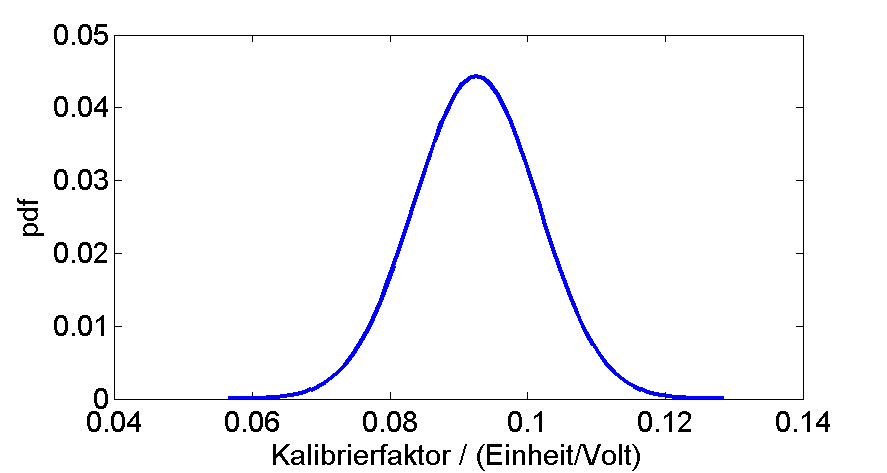
\includegraphics[width=100mm]{Bilder/Kalibrierfaktor.eps}
		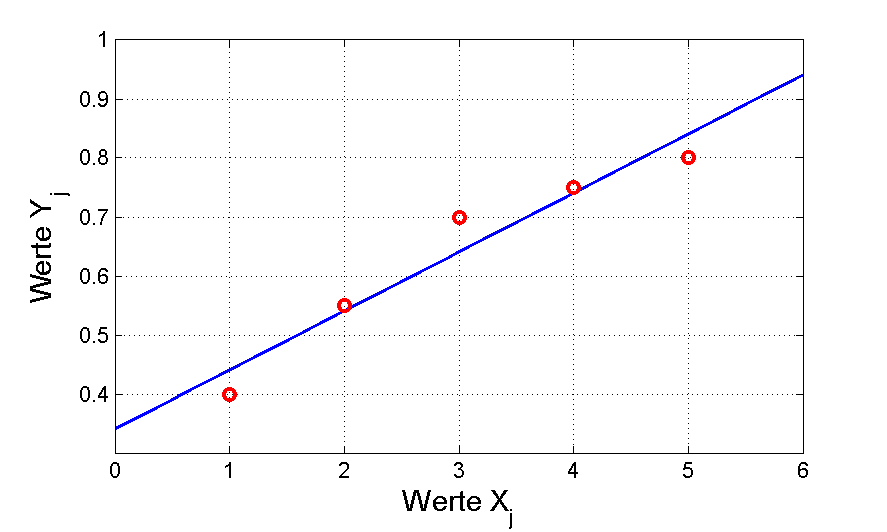
\includegraphics[width=140mm]{02_vorlesung/media/LinRegression.png}
		\caption{Lineare Regression. 
			Als Schätzparameter erhält man $\hat{\boldsymbol\theta} = [ 0.3400 ,0.1000 ]^T$}
		\label{fig:LineareRegression}
	\end{center}
\end{figure}

\textbf{Lösung zu Teil (b)} \\
Residuen: $\varepsilon_j = Y_j -(\hat\theta _0 + \hat\theta _1 \cdot X_j)$
mit $j=1,\ldots ,5$
\[\varepsilon_1 = -0.0400; \;\; \varepsilon_2 =  0.0100;\;\;
\varepsilon_3= 0.0600;\;\; \varepsilon_4 =0.0100;\;\;
\varepsilon_5 = -0.0400
\]
Qualitätsmaß:
\[
Q(\hat\theta _0,\hat\theta _1) = \sum\limits_{j = 1}^J {\varepsilon_j ^2 } 
= 0.0070
\]
Varianz der Residuen:
\[
s^2(\hat{\theta}_0 ,\hat{\theta}_1 ) = \frac{Q(\hat{\theta}_0 ,
	\hat{\theta}_1 )}{J - 2} = 0.0023 \quad \text{bzw.} \quad
s(\hat{\theta}_0 ,\hat{\theta}_1 ) = 0.048 
\]
Die Varianz der Residuen ist wie folgt gegeben:
\begin{equation}
\operatorname{Var}(\varepsilon) = \frac{1}{J-M} \cdot \left(\mathbf Y - \mathbf X \hat{\boldsymbol\theta}\right)^T 
\left(\mathbf Y - \mathbf X \hat{\boldsymbol\theta}\right)
\end{equation}
Die Kovarianzen der Schätzerparameter ${\boldsymbol\theta}$ 
sind gegeben durch:
\begin{equation}
\operatorname{Cov}(\boldsymbol\theta) = \left(\mathbf{X}^T \mathbf X \right)^{-1}
\operatorname{Var}(\varepsilon)
\end{equation}
Matlab-Code zur Bestimmung des Qualitätsmaßes und der Varianz
\begin{lstlisting}[style=Matlab]
% Qualitaetsmass Q
Q = (Y-X*thetaHat)' * (Y-X*thetaHat)
% Varianz der Residuen
Var_epsilon = 1/df *(Y-X*thetaHat)' * (Y-X*thetaHat)
% Wuzel aus Var_epsilon
RMSE = sqrt(Var_epsilon)
% Kovarianzen
Cov = Var_epsilon * inv(X'*X)
\end{lstlisting}
Als Ergebnis für unser Beispiel erhalten wir:\\
Q = 0.0070 \\
Var\_epsilon = 0.0023\\
RMSE = 0.0483 \\
Cov = \\
0.0026   -0.0007 \\
-0.0007    0.0002 \\

\textbf{Lösung zu Teil (c)} \\
Die Standardabweichung für $X$ berechnet sich zu $s_X = 1.5811$.

Für die Varianz des y-Abschnitt $\hat\theta_0$ ergibt sich: 
\begin{eqnarray}
\hat\sigma_{\theta_0}^2 &=& s^2(\hat{\theta}_0 ,\hat{\theta}_1 )
\left[\frac{1}{J} + \frac{\bar{X}^2}{(J-1)s_x^2 } \right]
\nonumber \\ 
&=& 
0.0023
\left[\frac{1}{5} + \frac{3^2}{(5-1)\cdot 1.5811^2 } \right]
\nonumber\\ 
&=& 0.00253 \nonumber
\end{eqnarray}
Damit ergibt sich die Standardabweichung für $\hat\theta_0$:
\[
s_{\hat\theta_0} = \sqrt{\hat\sigma_{\theta_0}^2} = 0.0503
\]
Für die Varianz der Steigung $\hat\theta_1$ ergibt sich: 

\begin{eqnarray}
\hat\sigma^2_{\theta_1} &=& \frac{ \hat s^2(\hat{\theta}_0 ,\hat{\theta}_1 )}
{s^2_X \cdot (J- 1) }
\nonumber \\
&=& \frac{ 0.0023}
{1.5811^2 \cdot (5- 1) } \nonumber \\
&=& 0.00023
\end{eqnarray}

Damit ergibt sich die Standardabweichung für $\hat\theta_1$
\[
s_{\hat\theta_1} = \sqrt{\hat\sigma_{\theta_1}^2} = 0.01517
\]

\newpage
\textbf{Anmerkung: Lösung mit Matlab/Octave} 
Bei Matlab gibt es den Befehl \glqq polyfit\grqq ~mit dem Polynomfits durchgeführt werden können. Matlab liefert hier dasselbe Ergebnis, auch für die Vertrauensbereiche, das Qualitätsmaß $Q$ (engl. SSE: Sum squared error) oder das Bestimmheitsmaß $\rho^2_{XY}$ (R-square), siehe Abb.\ref{fig:MatlabPolyfit}:
\begin{figure}[!htp]
	\begin{center}
		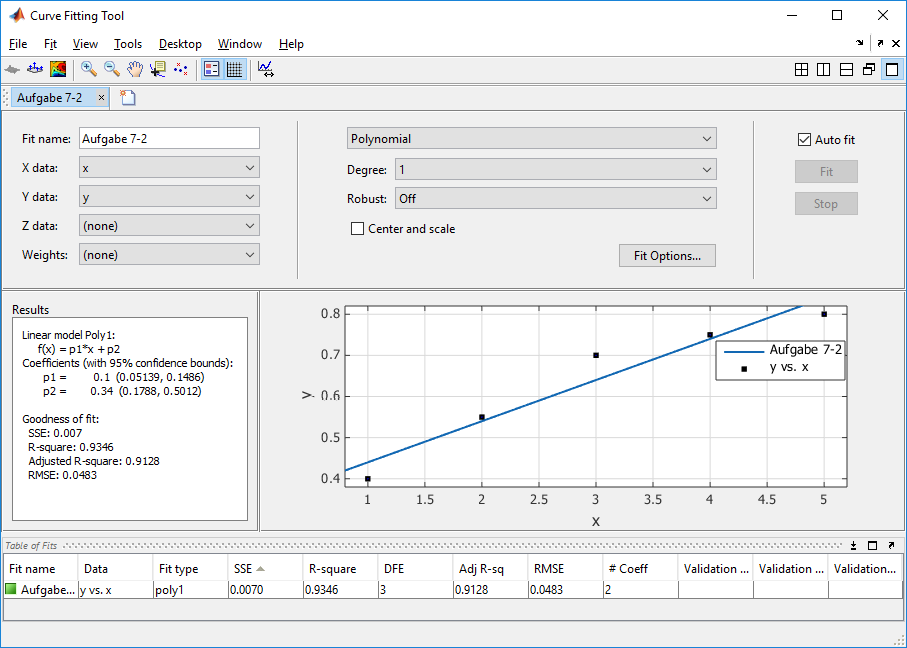
\includegraphics[width=160mm]{02_vorlesung/media/Matlab_CFTool.png}
		\caption{Lösung der Aufgabe mit dem polyfit Befehl von Matlab/Octave. 
			Es wird hier u.~a. der 95\%ige Vertrauensbereich berechnet und
			angezeigt (siehe Mitte links in der Abbildung).}
		\label{fig:MatlabPolyfit}
	\end{center}
\end{figure}

\textbf{Hinweis: Vertrauensbereich} \\
In einer der nächsten Vorlesungen werden wir sehen, wie man Vertrauensbereiche 
mit Hilfe der Varianzen bzw. Standardabweichungen berechnet. Dazu benötigt man 
noch die t-Verteilung. Da man hier 5 Messpunkte und 2 Modellparameter hat,
wird die t-Verteilung mit dem Freiheitsgrad 5-2 = 3 benötigt. 
95\%iger Vertrauensbereich für $\hat\theta_1$ mit $t_3 = 3.182$: 
\[
\varepsilon _{\hat{\theta}_1} = t_3 \cdot \hat\sigma_{\theta_1} = \frac{t_3 \cdot s(\hat{\theta}_0 ,
	\hat{\theta}_1 )}{s_X \cdot \sqrt {J
		- 1} } = 0.0486
\]
95\%iger Vertrauensbereich für $\hat\theta_0$ errechnet sich durch:
\[
\varepsilon _{\hat{\theta}_0} = t_3 \cdot \hat\sigma_{\theta_0} = t_3 \cdot s(\hat{\theta}_0 ,\hat{\theta}_1 ) \cdot \sqrt {\frac{1}{J} + \frac{\bar {X}^2}{(J - 1) s_X^2 }} = 0.1612
\]
\textbf{Ergebnis:} \\ 
Der 95\% Vertrauensbereich des Schätzwertes $\hat\theta_1$ ist somit gegeben durch:
\begin{equation}
\hat\theta_1 = 0.1000 \pm 0.0486 \quad \text{bzw.} \quad [0.0514;0.1486]
\end{equation}
Der 95\% Vertrauensbereich des Schätzwertes $\hat\theta_0$ ist somit gegeben durch: 
\begin{equation}
\hat\theta_1 = 0.3400 \pm 0.1612 \quad \text{bzw.} \quad [0.1788;0.5012]
\end{equation}


\begin{comment}
95\%iger Vertrauensbereich für $\hat\theta_1$ mit $t_3 = 3.182$ und 
Standardabweichung von $s_X = 1.5811$
\[
\varepsilon _{\hat{\theta}_1} = \frac{t_3 \cdot s(\hat{\theta}_0 ,
\hat{\theta}_1 )}{s_X \cdot \sqrt {J
- 1} } = 0.0486
\]
95\%iger Vertrauensbereich für $\hat\theta_0$ errechnet sich durch:
\[
\varepsilon _{\hat{\theta}_0} = t_3 \cdot s(\hat{\theta}_0 ,\hat{\theta}_1 ) \cdot \sqrt {\frac{1}{J} + \frac{\bar {X}^2}{(J - 1) s_X^2 }} = 0.1612
\]
\textbf{Ergebnis:} \\ 
Der 95\% Vertrauensbereich des Schätzwertes $\hat\theta_1$ ist somit gegeben durch:
\begin{equation}
\hat\theta_1 = 0.1000 \pm 0.0486 \quad \text{bzw.} \quad [0.0514;0.1486]
\end{equation}
Der 95\% Vertrauensbereich des Schätzwertes $\hat\theta_0$ ist somit gegeben durch: 
\begin{equation}
\hat\theta_1 = 0.3400 \pm 0.1612 \quad \text{bzw.} \quad [0.1788;0.5012]
\end{equation}
\end{comment}
\subsection{Fit einer kubischen Funktion (Polynom 3. Ordnung) mittels linearer Regression}
Wir nehmen wieder die gleichen Messwertpaare wie eben. Jedoch fitten wir 
nun eine kubische Funktion durch die Messdaten, d.h. 
\begin{equation}
Y = \hat{\theta_3} X^3 + \hat{\theta_2} X^2 + \hat{\theta_1} X^1 +
\hat{\theta_0} 
\end{equation}
Mit der Gl.(\ref{eq:schaetzwerte_fuer_theta}) können wir 
das Beispiel mit dem Matrixformalismus auch lösen. 
Die Regressormatrix $\boldsymbol X$ lautet:
\begin{equation}
	\boldsymbol{X} \; = \;
	\left(
	\begin{array}{cccc}
		1 & X_1 & X_1^2 & X_1^3 \\
		1 & X_2 & X_2^2 & X_2^3 \\
		1 & X_3 & X_3^2 & X_3^3\\
		1 & X_4 & X_4^2 & X_4^3\\
		1 & X_5 & X_5^2 & X_5^3
	\end{array}
	\right)
\end{equation}
Die Regressandenmatrix $\boldsymbol Y$ lautet:
\begin{equation}
	\boldsymbol{Y} \; = \;
	\left(
	\begin{array}{cc}
		Y_1 \\
		Y_2 \\
		Y_3 \\
		Y_4 \\
		Y_5 
	\end{array}
	\right)
\end{equation}
Die gesuchten Modellparameter sind: 
\[
\boldsymbol\theta = \left( 
\begin{array}{cc}
	\theta_0 \\
	\theta_1 \\
\end{array}
\right)
\]
Die optimalen Parameter $\boldsymbol{\hat \theta}$ ergeben sich durch Lösen
des folgenden Gleichungssystems, siehe Gl.(\ref{eq_Bestimmung_von_hat_theta})
\[
\boldsymbol{\hat \theta} \; = \;
\left( \mathbf{X}^\mathsf{T}  \, \mathbf{X} \right)^{-1} \mathbf{X}^\mathsf{T} \, \mathbf{Y}
\]

Als Ergebnis für die Schätzparameter erhalten wir dann: 
\[\hat{\boldsymbol\theta} = 
(0.1900, \;\; 0.2286,\;\; -0.0214, \;\; -0.0000) \]
Für das Qualitätsmaß ergibt sich: 
\[\mathrm{Q} = 5.7143e-04 \]
Für die Streuung der Residuen ergibt sich: 
\[\mathrm{Var\_epsilon} = 5.7143e-04 \]
Standardabweichung der Residuen: 
\[
\mathrm{RMSE} = 0.0239 \]
Die Kovarianzamtrix ergibt sich zu: 
\[
\operatorname{Cov} =
\begin{bmatrix}
0.0138  & -0.0176  &  0.0063  & -0.0007 \\
-0.0176 &   0.0236 &  -0.0087 &  0.0009 \\
0.0063  &  -0.0087 &   0.0033 &  -0.0004 \\
-0.0007 &   0.0009 &  -0.0004  &  0.0000
\end{bmatrix}
\]
Der Matlab/Octave-Code lautet (\href{https://mybinder.org/v2/gh/dhueser/MDA-Vorlesung-iprom-tu-bs/master?urlpath=/lab/tree/vorlesung/02_vorlesung/code/cubic_fit.ipynb}{Klicke hier für interaktive Session}): 
\lstinputlisting[style=Matlab]{02_vorlesung/code/cubic_fit.m}

Wir können auch die Curve Fitting Toolbox von Matlab 
verwenden, die uns das gleiche Ergebnis anzeigt:
\begin{figure}[!htp]
	\begin{center}
		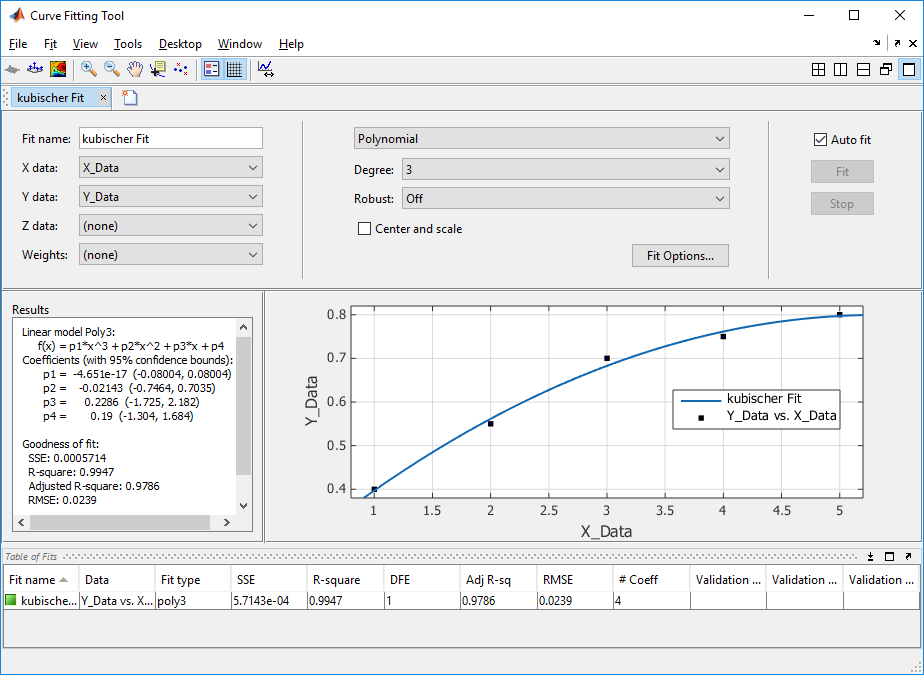
\includegraphics[width=150mm]{02_vorlesung/media/Matlab_CFTool_Kubischer_Fit.png}
		\caption{Kubischer Fit mit der Curve Fitting Toolbox von Matlab. 
			Zum jedem geschätzten Parameter wird der 95\%ige Vertrauensbereich 
			angegeben. Zu sehen sind u.a. das Qualitätsmaß Q (engl. SSE: Sum squared error), das Bestimmtheitsmaß $\rho^2_{XY}$ (engl. R-square), Standardabweichung der Residuen (engl. RMSE: root mean square error) und die Anzahl der Freiheitsgrade (engl. DFE, degree of freedom)}
		\label{fig:CFTool_kubischerFit}
	\end{center}
\end{figure}
\newpage

%Das vollständige Messergebnis für jeden der Regressionparameter ist damit
%\begin{equation}
%\theta_l \; = \;
%\boldsymbol{e}_l^\mathsf{T} \, \left( \mathbf{X}^\mathsf{T}  \, \mathbf{X} \right)^{-1} %\mathbf{X}^\mathsf{T} \, \mathbf{Y}
%\; \pm \; t_{1-\alpha/2, \nu} \, \hat \sigma_l
%\end{equation}
%mit $\nu = J-M$ und die Korrelationskoeffizienten für die Korrelation der %Regressionsparameter
%untereinander sind
%\begin{equation}
%\rho_{l,m} \; = \; \frac{\hat \sigma_{\varepsilon}^2}{\hat \sigma_l \, \hat \sigma_m} \; %\boldsymbol{e}_l^\mathsf{T} \, \left( \mathbf{X}^\mathsf{T}  \, \mathbf{X} \right)^{-1} %\, \boldsymbol{e}_m  .
%\end{equation}

\section{Aufgaben zum Selbststudium}
\subsection{1. Aufgabe zur Linearen Regression}
\label{Vorl2Regressionsaufg1}
Es wurde eine Stufe vermessen, die nominal eine Höhe von $100 \; \mathrm{\mu m}$ haben soll.
Die laterale Achse $x$ wird eingestellt (mit Präzisionstisch positioniert) 
und als Regressor betrachtet, also nicht als Zufallszahl.
Die vertikale Achse $z$ wird gemessen, als Regressand und damit als Zufallszahl
betrachtet.

\begin{center}
	\includegraphics[width=90mm]{02_vorlesung/media/uebungA5_step_plot.pdf}
\end{center}

%\vspace{2mm}

\begin{tabular}{l|c|c|c|c|c|c|c|c|c|c}
	\hline
	$x / \mathrm{mm}$ &
	0.00 & 0.25 & 0.50 & 0.75 & 1.00 & 1.25 & 1.50 & 1.75 & 2.00 & 2.25 \\
	\hline
	$z / \mathrm{\mu m}$ &
	-54.08 &-55.63 &-44.65 &-51.44 &-52.21 &-58.01 &-50.76 &-56.01 &-54.86 &-60.77\\ 
	\hline
\end{tabular}

\vspace{2mm}

\begin{tabular}{l|c|c|c|c|c|c|c|c|c|c|c}
	\hline
	$x / \mathrm{mm}$  & 2.50 &
	2.75 & 3.00 & 3.25 & 3.50 & 3.75 & 4.00 & 4.25 & 4.50 & 4.75 & 5.00 \\
	\hline
	$z / \mathrm{\mu m}$ &36.85 &38.02 &31.71 &36.21 &23.39 &29.01 &30.11 &29.35 &20.81 &33.27 &23.19\\
	\hline
\end{tabular}

\vspace{2mm}

Die Modellgleichung, mit der die Stufe beschrieben wird, ist
$$
z_j \; = \; a \, x_j \, + \, c \, + \, h \, \delta_{j \in C} \; + \; \varepsilon_j
$$
mit $C$ Menge der Indizes von 1 bis $J_C$. Hier sei $J_C = 10$:
$$
C \; = \; \{\, j \, | \, j = 1, 2, \dots, J_C \}
$$
und
$$
\delta_{j \in C} \; = \; \left\{
\begin{array}{ll}
1 & \mathrm{falls} \; \;  j \in C \; \mathrm{~d.h.~} j = 1 \; \mathrm{~oder} \; j = 2
\mathrm{~oder} \; \dots \; j = J_C\\
0 & \mathrm{sonst}
\end{array} \right.
$$
Dabei ist $h$ noch nicht die Stufenhöhe, sondern deren Projektion auf die vertikale Achse.
Die Stufenhöhe $d$ ist der senkrechte Abstand zwischen den beiden parallelen Geraden, die jeweils durch die Punkte auf dem oberen und dem unteren Niveau gehen.

\begin{itemize}
	\item[a)] Stellen Sie das lineare Gleichungssystem auf, das sich durch partielles Ableiten
	für das Optimierungsproblem
	$$
	\min\limits_{a,c,h} \left\{\sum_{j=1}^{J_T} \varepsilon_j^2\right\}
	$$
	ergibt, mit $J_T = 21$.
	\item[b)] Schreiben Sie die Gleichung für die Stufenhöhe $d$ als Funktion von $h$ und $a$ auf.
	\item[c)] Schreiben Sie die Gleichung für die Varianz der Residuen auf.
	\item[d)] Schreiben Sie die Formel für die Kovarianzmatrix der Modellparameter
	$a, c, h$ auf.
	\item[e)] Verwenden Sie eine Programmierumgebung Ihrer Wahl, Matlab, Octave, Python, R, ...
	die Ihnen einen Solver für lineare Gleichungssysteme zur Verfügung stellt, sowie
	eine Routine zur Matrixinversion und berechen Sie die Zahlenwerte für die Modellparameter
	sowie deren Kovarianzmatrix.
\end{itemize}
Anmerkung: Die inverse Matrix brauchen Sie nicht analytisch zu berechnen, sondern
	lediglich $(...)^{-1}$ zu notieren.

%
\chapter{Optimierung nichtlinearer Modelle}
\label{nonlinOpti}
\section{Konzepte von Optimierungsverfahren für nichtlineare Modelle}
Während dieser Vorlesungsreihe beleuchten wir die Thematik physikalische Größen zu ermitteln, die
indirekt zugänglich sind. Sie werden über eine Modellbildung als Modellparameter approximiert.
In den bisherigen Kapiteln hatten wir uns damit befasst, Modellparameter linearer Modelle, zu schätzen.
Die Besonderheit dabei ist, dass die \textsl{Kostenfunktion} $Q$ eine lineare Abhängigkeit von den
Modellparametern hat, so dass die Modellparameter
im Fall der Ausgleichsrechnung nach der Methode der kleinsten Quadrate durch Lösen eines
linearen Gleichungssystems ermittelt werden können.
Im vorangegangen Kapitel wurde in Gl.~(\ref{linRegGleichungssystem}), Gl.~(\ref{GleichungssytemKostenfkt})
 und Gl.~(\ref{LsgRegressionGlSys}) gezeigt, dass das Gleichungssystem
aufgestellt wird, indem der Gradient, der die Kostenfunktion nach den Modellparametern ableitet, gleich Null
gesetzt wird, um das Maximum zu finden.

Für den Fall, dass die Modellparameter nicht linear in die Kostenfunktion $Q$,
auch \textsl{Zielfunktional} genannt, eingehen,
erfolgt die Schätzung der Modellparameter durch Variation, also durch Optimierung derart, um
das Minimum der Optimierungszielfunktion $Q$ zu finden.

Wir sind von normalverteilten Abweichungen ausgegangen und haben uns
die Likelihoodverteilungen angeschaut. Als Beispiel nehmen wir ein Modell mit 2 Parametern, bei
dem eine Gerade durch den Ursprung des Koordinatensystems eines dreidimensionalen
Raums gehe und bei dem alle drei Achsen von der gleichen physikalischen Dimension seien.
Die beiden zu schätzenden Parameter seien hier der Azimutalwinkel $\alpha$ und der
Polarwinkel $\theta$, die die gesuchte Richtung der Geraden beschreiben.
Ein Punkt $\mathbf{r}$, der exakt auf der Geraden liegt, erfülle
\begin{equation}
\mathbf{r} \; = \; \lambda \mathbf{u} \qquad \mathrm{mit} \qquad
\mathbf{u}(\alpha,\theta) \; = \; \left(\begin{array}{c}
\cos(\alpha) \sin(\theta)\\
\sin(\alpha) \sin(\theta)\\
\cos(\theta) \end{array}\right) \qquad \mathrm{und} \qquad \lambda \in I \!\! R.
\end{equation}
\begin{figure}
\begin{center}
\includegraphics[width=0.95\textwidth, angle = 0]{03_vorlesung/media/LSopti_example1.pdf}
\end{center}
\caption{Modell mit 2 zu schätzenden Parametern (\textsl{links}) und der dazugehörigen
Likelihood für normalverteilte Residuen (\textsl{rechts}).\label{LSoptiExample1}}
\end{figure}

Abb.~\ref{LSoptiExample1} zeigt das Modell als schwarz gestrichelte Gerade und die Beobachtungen als blaue Kreise, sowie rechts die Likelihoodverteilung. Wir hatten bereits ausführlich darüber gesprochen, dass die Suche des Maximums der Likelihood in die Suche des Minimums übergeht. Es gelte nun diejenige Geradenrichtung zu finden, für die die senkrechten Abstände,
die Residuen $\varepsilon_j$,  der beobachteten Punkte (Messpunkte) $\mathbf{r}_{\mathrm{Mess},j} = (X_{1,j}, X_{2,j}, X_{3,j})^\mathsf{T}$ minimal sind. Für das Kriterium für minimale Abstände, also die Kostenfunktion $Q$, setzen wir wieder voraus, dass die Messpunkte gaußverteilt um eine Gerade streuen. Den Betrag für die senkrechten Abstände berechnen wir mit
\begin{equation}
\varepsilon(\alpha,\theta)_j \; = \; \left| \mathbf{r}_{\mathrm{Mess},j} \; - \;
( \mathbf{r}_{\mathrm{Mess},j} \cdot \mathbf{u}(\alpha,\theta) ) \, \mathbf{u}(\alpha,\theta) \right|
\end{equation}
mit $|$ als Betrag gemäß $| \mathrm{a} | = \sqrt{a_1^2 + a_2^2 + a_3^2}$.
Für die Likelihoodverteilung auf der rechten Seite von Abb.~\ref{LSoptiExample1} verwenden wir
die Wahrscheinlichkeitsdichte gemäß
\begin{equation}
p(\varepsilon_1,\dots,\varepsilon_J | \alpha, \theta)
\propto e^{-\frac{1}{2} \, \sum\limits_{j=1}^J \, \left(\frac{\varepsilon(\alpha,\theta)_j}{\sigma} \right)^2} .
\end{equation}
Für den Schätzvorgang wählen wir wieder für das Zielfunktional $Q$ die Summe der Quadrate der Residuen $Q = \sum \varepsilon_j^2$,
also einen Optimierungsvorgang gemäß der Methode der kleinsten
Residuenquadratsumme (RQS).
\begin{equation}
\min_{\alpha,\theta} \, \sum\limits_{j=1}^J \, \varepsilon(\alpha,\theta)_j^2 .
\end{equation}
Die Optimierungsrechnung bietet sehr unterschiedliche Methoden für eine Minimumsuche.

Wir können sie grob danach einteilen
\begin{itemize}
\item ob das nächste Modellparametertupel gemäß einer gewissen Strategie aus
mehreren Vor\-gänger\-tupeln mit den dazugehörigen Werten der Kostenfunktion $Q$ gewonnen wird
\item oder ob nicht nur die Kostenfunktion $Q$ direkt, sondern auch deren Gradienten bestimmt
werden.
\end{itemize}
Ein möglicher, vielfach genutzer Ansatz für das Verwenden mehrerer Vorgängertupel mit den dazugehörigen Werten der RQS
ist die \textbf{Simplexmethode nach Nelder und Mead} aus dem Jahr 1965. Er wird als Bibliotheksfunktion \texttt{fminsearch} in Gnu-Octave oder
in Matlab zur Verfügung gestellt. Mit Simplex ist ein Vieleck gemeint, das $M+1$ Ecken hat für $M$
Parameter, in unserem Beispiel also drei Ecken für zwei Parameter, was in Abb.~\ref{LSoptiExample1NM} durch
schwarz umrandete weiße Punkte, die mit schwarzen, durchgezogenen Linien verbunden sind, skizziert ist. Zum Aufbau eines
Startsimplex wird ein Startwerttupel $\mathbf{p}_{0,0}$ des Modellparametervektors gewählt und zu jedem Parameter ein
weiterer Vektor, der eine Variation $\Delta P_m$ repräsentiert:
\begin{equation}
\mathbf{p}_{0,1} \; = \; \mathbf{p}_{0,0} \; + \; \left(\begin{array}{c}
\Delta P_1 \\
0 \\
\vdots \\
0
\end{array}\right) \qquad
\mathbf{p}_{0,m} \; = \; \mathbf{p}_{0,0} \; + \; \left(\begin{array}{c}
0 \\
\vdots \\
0 \\
\Delta P_m \\
0 \\
\vdots \\
0
\end{array}\right) \qquad
\mathbf{p}_{0,M} \; = \; \mathbf{p}_{0,0} \; + \; \left(\begin{array}{c}
0 \\
\vdots \\
0 \\
\Delta P_M
\end{array}\right)
\end{equation}
\begin{figure}
\begin{center}
\includegraphics[width=0.6\textwidth, angle = 0]{03_vorlesung/media/LSopti_example1_LS_NM.pdf}
\end{center}
\caption{Residuenquadratsumme des Beispielmodells mit 2 zu schätzenden Parametern
und Simplex für Optimierungsverfahren nach Nelder und Mead.\label{LSoptiExample1NM}}
\end{figure}

Die Strategie ist es, diesen Simplex durch Zusammenziehen oder durch Umklappen dazu zu bewegen, in
die Minimumsmulde herunter zu klettern, was in Abb.~\ref{LSoptiExample1NM} durch hellgrau umrandete
weiße Punkte und durch Pfeile skizziert ist. Die Entscheidung, wann er sich zusammen zieht und dadurch
auch verkleinert und wann er umklappt und wann er notfalls auch wieder gestreckt (vergrößert) werden
muss wird anhand dessen getroffen, ob die Werte des Zielfunktionals $Q$ kleiner werden oder nicht.
Wenn er klein und flach im Tal angekommen ist, terminiert der Algorithmus. Hierzu gibt es dann noch
verschiedene Ansätze, wie überprüft wird, ob er zu weit über dem Tal waagerecht festhakt und eigentlich
noch eine zu große Mulde darunter liegt und eines der Simplexbeine angezogen werden muss.

Dieses Verfahren eignet sich auch für zu minimierende Zielfunktionale, die nicht so schön stetig
differenzierbar, d.h.\ glatt, in der Talmulde sind. Für Messungen mit Beobachtungen, die nicht gaußverteilt
streuen, sondern stark abweichende Punkte aufweisen, greift man auf andere Verteilungen zurück.
Eine mögliche Verteilung kann die Laplaceverteilung sein
\begin{equation}
p(\varepsilon_1,\dots,\varepsilon_J | \alpha, \theta)
\propto e^{-\frac{1}{2} \, \sum\limits_{j=1}^J \, \frac{| \varepsilon(\alpha,\theta)_j |}{\sigma} }
\end{equation}
was bedeutet, dass sie eine Exponentialverteilung der Absolutbeträge der
Residuen ist. Bei dem zu minimierenden Exponenten
\begin{equation}
\min_{\alpha,\theta} \, \sum\limits_{j=1}^J \, | \varepsilon(\alpha,\theta)_j |
\end{equation}
bildet sich die Minimumsmulde durch die Betragsbildung zu einer ausgeprägt scharfen Spitze aus.
Im Minimum gibt es also keine einheitliche Steigung. Je nach Richtung, von der man sich ihr nähert,
gibt es sehr unterschiedliche Steigungen, was soviel bedeutet wie die Nichtstetigkeit der
Steigungsfunktion. Steigungen im mehrdimensionalen Raum heißen Gradienten. Die Gradientenfunktion
ist nicht stetig, die Funktion selber also nicht stetig differenzierbar. Für das Simplexverfahren
spielt dies aber keine Rolle. Das Simplexverfahren hat aber den Nachteil, dass es sehr
empfindlich darauf reagiert, welchen Startsimplex man zu Beginn auswählt. Es kann dadurch
im harmlosen Fall relativ langsam werden, aber im ungünstigsten Fall in die Irre laufen und gar
nicht konvergieren. Auch kann das Problem des Festhakens bei Optimierungsaufgaben mit vielen
Parametern zu einem schwerwiegenderen werden.

\begin{figure}
\begin{center}
\includegraphics[width=0.95\textwidth, angle = 0]{03_vorlesung/media/LSopti_example1_LS_Grad.pdf}
\end{center}
\caption{Residuenquadratsumme des Beispielmodells mit 2 zu schätzenden Parametern
und Gradienten eingezeichnet als Pfeile (\textsl{links}) und Beträge der
Gradienten als Funktion der 2 zu schätzenden Parameter (\textsl{rechts}).\label{LSoptiExample1Grad}}
\end{figure}
Für zu minimierende Zielfunktionale wie wir sie bei normalverteilten Residuen, also bei
den rundlichen, stetig differenzierbaren Kostenfunktionen als Residuenquadratsummen haben, können wir Verfahren
einsetzen, die nicht nur die Kostenfunktion $Q$ direkt, sondern auch deren Gradienten $\nabla Q$ verwenden.
Hierzu wird \textsl{ein} Startwertetupel (nicht wie bei der Simplexmethode $M+1$)
für die Modellparameter gebracht. Es wird der Gradient, also die Richtung des steilsten
Abhangs der Kostenfunktion zusammen mit dem Wert der Steigung an der Position des Startwerttupels
bestimmt. Dieses Verfahren beleuchten wir im folgenden Abschnitt anhand unseres Beispiels etwas genauer.

\section{Gradientenverfahren für nichtlineare Zielfunktionale}

Das Gradientenverfahren braucht wie alle anderen Methoden zur Schätzung von Parametern, die
nicht linear in die Residuen eingehen, ein Tupel von Startwerten der Parameter, was wir in
Abb.~\ref{LSoptiExample1Grad} als schwarz umrandeten weißen Punkt dargestellt haben.
In Abb.~\ref{LSoptiExample1Grad} ist die Idee illustriert, wie sich die Position des
Parametervektors verändert. Die Änderungsvektoren $\Delta \mathbf{p}$ werden aus der Richtung
des steilsten Abhangs ermittelt, wie durch die Pfeile mit gestrichtelter Linie skizziert.
Der Gradient des Betrags eines Residuums an der Stelle des Startwertevektors $(\alpha_0, \theta_0)$
ist der Vektor der partiellen Ableitungen
\begin{equation}
\left. \nabla_{\alpha,\theta} \varepsilon_j \right|_{\alpha_0, \theta_0} \; = \;
\left(\begin{array}{c}
\frac{\partial}{\partial \alpha} \\
\frac{\partial}{\partial \theta}
\end{array}\right) \left. \varepsilon_j \right|_{\alpha_0, \theta_0} .
\end{equation}
Das auf die Spitze gestellte Dreieck heißt Nablaoperator.
Die Schreibweise $|_{\alpha_0, \theta_0}$ lesen wir \glqq an der Stelle\grqq ~$(\alpha_0, \theta_0)$.
Für die Minimierung bestimmen wir die Stelle $(\hat \alpha, \hat \theta)$, an der sich die Talsohle
der Mulde der RQS-Funktion befinden. Anders gesagt suchen wir die Position im Modellparameterraum,
die unten in der Mulde RQS-Funktion liegt,
in der keine Steigung mehr vorhanden ist, d.h.\ der Gradient ein Nullvektor ist, d.h.
\begin{equation}
\lim_{\alpha \rightarrow \hat \alpha, \theta \rightarrow \hat \theta}
\left\{\nabla_{\alpha,\theta} \,
\sum\limits_{j=1}^J \, \varepsilon(\alpha,\theta)_j^2
\right\} \; = \;
\left(\begin{array}{c}
0 \\
0
\end{array}\right) .
\label{LSschaetzung1}
\end{equation}
Hierbei müssen wir uns aber darüber im Klaren sein, dass Gradient gleich Nullvektor nicht nur
bei einem Minimum vorliegt, sondern auch bei einem Maximum und bei einem Sattelpunkt, weshalb wir
im letzten Abschnitt ein Verfahren kurz vorstellen, das sich mit dieser Problematik besser
auseinander setzt.

Wir ziehen den Nablaoperator in die Summe rein und
verwenden die Kettenregel, äußere Ableitung mal innere Ableitung:
\begin{equation}
\nabla_{\alpha,\theta} \,
\sum\limits_{j=1}^J \, \varepsilon(\alpha,\theta)_j^2
 \; = \;
\sum\limits_{j=1}^J \, \nabla_{\alpha,\theta} \, \varepsilon(\alpha,\theta)_j^2
 \; = \;
2 \, \sum\limits_{j=1}^J \, \varepsilon(\alpha,\theta)_j \nabla_{\alpha,\theta} \, \varepsilon(\alpha,\theta)_j
 \; \overset{!}{=} \;
\left(\begin{array}{c}
0 \\
0
\end{array}\right) .
\label{GradientQ2params}
\end{equation}

Die beiden Parameter $\alpha,\theta$ fassen wir zusammen in einen Parametervektor $\mathbf{p}$ und
betrachten im folgenden den Allgemeinfall für $M$ Parameter $\mathbf{p} = (P_1,\dots,P_M)^\mathsf{T}$.
Die Residuen sind dann jeweils Funktion des Parametervektors
$\boldsymbol \varepsilon(\mathbf{p}) = (\varepsilon_1(\mathbf{p}), \dots, \varepsilon_J(\mathbf{p}))^\mathsf{T}$,
so dass die Kostenfunktion $Q$ entsprechend Funktion des Parametervektors ist
\begin{equation}
Q(\mathbf{p}) \; = \; \boldsymbol \varepsilon^\mathsf{T}(\mathbf{p}) \, \boldsymbol \varepsilon(\mathbf{p}),
\label{Zielfunktional}
\end{equation}
für die wir das Minimum suchen mit
\begin{equation}
\min_{\mathbf{p}} \left\{ Q(\mathbf{p}) \right\}
\end{equation}
indem wir nach dem Nullstellenvektor der Gradientenfunktion
\begin{equation}
\nabla_{\mathbf{p}} Q(\mathbf{p}) \; = \;
 2 \, \boldsymbol \varepsilon^\mathsf{T} \, \left( \nabla_{\mathbf{p}}^\mathsf{T} \boldsymbol \varepsilon \right)
\label{ZielfunktionalGrad}
\end{equation}
suchen, für den $Q$ ein Minimum und nicht ein Maximum oder Sattelpunkt annimmt.\\
(Hinweis zu Gl.~(\ref{ZielfunktionalGrad}): $\frac{\partial}{\partial p} \varepsilon^2(p) =
2 \varepsilon(p) \frac{\partial}{\partial p} \varepsilon(p)$ )\\
Dabei ist $\nabla_{\mathbf{p}}$ Spaltenvektor und $\nabla_{\mathbf{p}}^\mathsf{T}$ Zeilenvektor
mit den partiellen Ableitungsoperatoren $\frac{\partial}{\partial P_m}$.
Wir suchen dasjenige $\mathbf{p}$ für das
\begin{equation}
\lim_{\mathbf{p} \rightarrow \mathbf{\hat p}}
\nabla_{\mathbf{p}} Q(\mathbf{p}) \; = \; \left(\begin{array}{c} 0\\ \vdots \\ 0 \end{array}\right)
\label{ZielfunktionalGrad1}
\end{equation}
Bei der Suche nach dem Minimum wird mit einem Tupel von Parametern angefangen, also
mit einem Startwertvektor $\mathbf{p}_0$. Dann wird ein Schrittvektor $\Delta \mathbf{p}_0$ ermittelt,
der gegangen wird, um
zu einem Nachfolgepunkt im Raum der Modellparamter zu gelangen $\mathbf{p}_1 = \mathbf{p}_0 + \Delta \mathbf{p}_0$.
Dies erfolgt solange, bis der Parametervektor beliebig dicht an das Minimum von $Q$ gelangt sind. Es gibt damit eine
gewisse Anzahl $K$ von Iterationschritten, derart dass der Vektor $\mathbf{p}_K = \mathbf{\hat p}$ für minimales
$Q$ als Tupel von Schätzwerten für die Modellparameter verwendet wird.
Die einzelnen Iterationsschritte $\kappa$ bedeuten eine Revision des Modellparametervektors
\begin{equation}
\mathbf{p}_\kappa = \mathbf{p}_{\kappa-1} + \Delta \mathbf{p}_{\kappa-1}
\label{Revisionsschritt}
\end{equation}
mittels \textsl{Inkrementvektoren}
$\Delta \mathbf{p}_1, \dots, \Delta \mathbf{p}_{\kappa}, \dots, \Delta \mathbf{p}_{K-1}$.

Wir nehmen eine Taylorreihenentwicklung vor, über die wir die Gradientenfunktion des Zielfunktionals
als lineare Funktion eines \textsl{Inkrementvektors} $\Delta \mathbf{p}$ darstellen. Dazu entwickeln
wir die Residuen $\varepsilon_j$ in Taylorreihe bis zum linearen Term
\begin{equation}
\left(\begin{array}{c}
\varepsilon_1(\mathbf{p}) \\
\vdots \\
\varepsilon_j(\mathbf{p}) \\
\vdots \\
\varepsilon_J(\mathbf{p})
\end{array}\right)
\; = \;
\left(\begin{array}{c}
\varepsilon_1(\mathbf{p}_\kappa) \; + \; \nabla_{\mathbf{p}} \left. \varepsilon_1 \right|_{\mathbf{p}_\kappa} \cdot \Delta \mathbf{p}\\
\vdots \\
\varepsilon_j(\mathbf{p}_\kappa) \; + \; \nabla_{\mathbf{p}} \left. \varepsilon_j \right|_{\mathbf{p}_\kappa} \cdot \Delta \mathbf{p}\\
\vdots \\
\varepsilon_J(\mathbf{p}_\kappa) \; + \; \nabla_{\mathbf{p}} \left. \varepsilon_J \right|_{\mathbf{p}_\kappa} \cdot \Delta \mathbf{p}
\end{array}\right).
\label{TaylorResi1}
\end{equation}
Hier bilden die partiellen Ableitungen der einzelnen Residuen nach allen Parametern eine $J \times M$-Matrix, die \textsl{Jakobimatrix}
genannt wird:
\begin{equation}
\boldsymbol{J}^{(\kappa)} \; = \; \left(\begin{array}{ccc}
\left. \frac{\partial \varepsilon_1}{\partial P_1} \right|_{\mathbf{p}_\kappa} & \dots & \left. \frac{\partial \varepsilon_1}{\partial P_M} \right|_{\mathbf{p}_\kappa} \\
 & \ddots & \\
\left. \frac{\partial \varepsilon_J}{\partial P_1}\right|_{\mathbf{p}_\kappa} & \dots & \left. \frac{\partial \varepsilon_J}{\partial P_M}\right|_{\mathbf{p}_\kappa}
\end{array}\right) ,\; \textrm{bzw.} \; J_{jm}^{(\kappa)}= \left. \frac{\partial \epsilon_j}{\partial p_m}\right|_{\mathbf{p}_\kappa}
\;\textrm{mit} \; j=1\ldots J; \;\; m=1\ldots M.
\end{equation}
Der hochgestellte und in Klammern gesetzte Index $\kappa$
an dem Symbol für die \textsl{Jacobimatrix}, soll bedeuten,
dass dies die \textsl{Jacobimatrix} für den Parametervektor an der Stelle
$\mathbf{p}_\kappa$ ist, also für die Position der Modellparameter beim $\kappa$-ten Interationsschritt.
Der Begriff Jacobimatrix bedeutet nur, dass es
sich um eine Matrix partieller Ableitungen handelt.
\begin{quote}
Die \textsl{Jacobimatrix} (benannt nach Carl Gustav Jacob Jacobi; auch
\textsl{Funktionalmatrix}, \textsl{Ableitungsmatrix} oder \textsl{Jacobische} genannt)
einer differenzierbaren Funktion
$f\colon I \! \! R^{n} \mapsto I \! \! R ^{m}$ ist die
$m\times n$-Matrix sämtlicher erster partieller Ableitungen.
\end{quote}


Einsetzen dieser Jacobimatrix in Gl.~(\ref{TaylorResi1}) liefert dann
\begin{equation}
\left(\begin{array}{c}
\varepsilon_1(\mathbf{p}) \\
\vdots \\
\varepsilon_J(\mathbf{p})
\end{array}\right)
\; = \;
\left(\begin{array}{c}
\varepsilon_1(\mathbf{p}_\kappa) \\
\vdots \\
\varepsilon_J(\mathbf{p}_\kappa)
\end{array}\right)
\; + \; \boldsymbol{J}^{(\kappa)} \Delta \mathbf{p} .
\label{TaylorResi2}
\end{equation}
Wir schreiben Gl.~(\ref{TaylorResi2}) in Vektorschreibweise, mit $\boldsymbol{\varepsilon}$ hier als Spaltenvektor
der einzelnen Residuen.
\begin{equation}
\boldsymbol{\varepsilon}(\mathbf{p})
\; = \;
\boldsymbol{\varepsilon}(\mathbf{p}_\kappa)
\; + \; \boldsymbol{J}^{(\kappa)} \Delta \mathbf{p} .
\label{TaylorResi3}
\end{equation}
Ferner setzen wir die Jacobimatrix in Gl.~(\ref{ZielfunktionalGrad}) ein
\begin{equation}
\frac{1}{2} \nabla_{\mathbf{p}} Q(\mathbf{p})  \; = \; \boldsymbol{\varepsilon}^\textsf{T}(\mathbf{p})
 \, \boldsymbol{J}
\label{ZielfunktionalGradJ}
\end{equation}
% \; \overset{!}{=} \; \left(\begin{array}{c} 0\\ \vdots \\ 0 \end{array}\right)
% \label{GradientQv}
Wir setzen die Reihenentwicklung der Residuen Gl.~(\ref{TaylorResi3}) ein und
den Gradienten Gl.~(\ref{ZielfunktionalGradJ}) in Gl.~(\ref{ZielfunktionalGrad1}) ein.
So erhalten wir ein in $\Delta \mathbf{p}$ lineares Gleichungssystem:
\begin{equation}
\left( \boldsymbol{\varepsilon}(\mathbf{p}_\kappa)
\; + \; \boldsymbol{J}^{(\kappa)} \Delta \mathbf{p}_\kappa \right)^\textsf{T} \, \boldsymbol{J}^{(\kappa)}
\; \overset{!}{=} \; \left( 0 \dots  0 \right)
\label{GradientQlinGl1}
\end{equation}
wobei hier der Nullvektor wie der transponierte Modellparametervektor ein
Zeilenvektor im $I \! \! R^{M}$ ist.
Wir formen diese Gleichung, die in Zeilenvektorschreibweise ist, um in
\begin{equation}
\left( \boldsymbol{J}^{(\kappa)} \Delta \mathbf{p}_\kappa \right)^\textsf{T} \, \boldsymbol{J}^{(\kappa)}
\; \overset{!}{=} \;
- \boldsymbol{\varepsilon}(\mathbf{p}_\kappa)^\textsf{T} \, \boldsymbol{J}^{(\kappa)}
\label{GradientQlinGl2}
\end{equation}
und transponieren diese, um sie als lineares Gleichungssytem mit Spaltenvektoren vorliegen zu haben
d.h.
\begin{equation}
 \boldsymbol{J}^{(\kappa) \textsf{T}} \, \boldsymbol{J}^{(\kappa)} \, \Delta \mathbf{p}_\kappa
\; \overset{!}{=} \;
-  \boldsymbol{J}^{(\kappa) \textsf{T}} \, \boldsymbol{\varepsilon}(\mathbf{p}_\kappa) .
\label{GradientQlinGl3}
\end{equation}
Die Lösung dieses linearen Gleichungssystems liefert den Inkrementvektor $\Delta \mathbf{p}_\kappa$,
mit dem wir den Schritt zur nächsten Position $\mathbf{p}_{\kappa+1} \; = \; \mathbf{p}_{\kappa} \, + \,
\Delta \mathbf{p}_{\kappa}$ gehen. Die Iterationen enden, wenn der Betrag der Gradientenfunktion oder
das Quadrat nahe Null, also kleiner als eine sehr kleine Zahl $\varepsilon$ ist:
\begin{equation}
 \boldsymbol{\varepsilon}(\mathbf{p}_\kappa)^\mathsf{T}
\, \boldsymbol{J}^{(\kappa)} \, \boldsymbol{J}^{(\kappa) \textsf{T}} \, \boldsymbol{\varepsilon}(\mathbf{p}_\kappa) \;
< \; \varepsilon
\end{equation}

Für Kostenfunktionen, die wie in Abb.~\ref{LSoptiExample1Grad}, ein sauber ausgeprägtes Minimum
haben, und für die ein Startwerttupel zu den Modellparametern, das nah genug an der Mulde dran ist und
sehr weit weg von irgendwelchen Maxima und Sattelpunkten, lässt sich auf diese Weise das Minimum
finden.

\section{Beispiel zu Gradienten-Verfahren nach Gauß-Newton für den Fall gleicher Varianzen}

Gegeben ist die Gl.(\ref{GradientQlinGl3}) mit
\[
 \boldsymbol{J}^{(\kappa) \textsf{T}} \, \boldsymbol{J}^{(\kappa)} \, \Delta \mathbf{p}_\kappa
\; \overset{!}{=} \;
-  \boldsymbol{J}^{(\kappa) \textsf{T}} \, \boldsymbol{\varepsilon}(\mathbf{p}_\kappa)
\]
zur Bestimmung der Modellparameter. Mit dieser Gleichung wird mit jeder Iteration die Änderung des Modellparameters
$\Delta \mathbf{p}_\kappa$ bestimmt. Nach jeder Iteration $\kappa$  erhält man einen neuen Modellparameter  $\mathbf{p}_{\kappa +1}$ erhält.
\[
\mathbf{p}_{\kappa+1} \; = \; \mathbf{p}_{\kappa} \, + \,
\Delta \mathbf{p}_{\kappa}
\]

Die Optimierung endet entweder wenn die Residuen kleiner sind als vorgegeben oder
bei einer vorgegebenen Interationsanzahl.
Die Jakobimatrix $J$ sind die partiellen Ableitungen (=Gradienten) nach den
Modellparametern $\boldsymbol{p}$:
\[ (\mathbf{J})_{jl} = \frac{\D \partial \varepsilon_j (\boldsymbol p_{(\kappa)})}{\D \partial  p_l}\]
Hierbei läuft der Index der Wertepaare von $j=1,\ldots,J$  und der Index
der gesuchten Modellparamter von $l=1,\ldots,M$.
(Weitere Infos zum Gauß-Newton Verfahren, siehe z.B. \cite{Wiki02})

Die Gl. (\ref{GradientQlinGl3}) kann in einen Programmiercode
umgesetzt werden.

\textbf{Algorithmus des Gauß-Newton-Verfahrendes}

Input: Startwert: $\boldsymbol p_0$, Zielfunktional $F(p_\kappa):= \boldsymbol\epsilon (\boldsymbol p^{(\kappa)}) $, Partielle Ableitungen $F'(\boldsymbol p_{\kappa}) := \mathbf J$ \\
\hspace*{1em}\textit{for} $\kappa = 0,1, \ldots$ \\[-3ex]
\begin{itemize}
	\item[i)] Berechne $F(\theta_\kappa)$, $F'(\theta_\kappa)$
	\item[ii)] Bestimme den Korrekturvektor~$s_\kappa := \Delta \boldsymbol p^{(\kappa)}$~über~
	$F^\prime(x_k)^T\;F^\prime(x_\kappa)\; s_\kappa = -F^\prime(x_\kappa)^T\;F(x_\kappa)$
	\item[iii)] Setze~$\boldsymbol p_{\kappa+1} = \boldsymbol p_\kappa + s_\kappa$
\end{itemize}
\hspace*{1em}\textit{end} \\

Eine einfache mögliche Realisierung in Octave-/Matlab ist nachfolgend dargestellt:
\begin{verbatim}
	function theta = gauss_newton(F,DF,p0,maxit,tol)
	% F: Zielfunktional,DF:Ableitung des Zielfunktionals (Jakobimatrix)
	% p0: Startwerte für die gesuchten Modellparamter
	% maxit: Anzahl der maximalen Iterationen
	% tol: Toleranz / Residuum
	k=0;
	p=p0;
	s=-(DF(p0)'*DF(p0))\(DF(p0)'*F(p0));
	while norm(s)>tol && k<maxit
	k=k+1;
	p=p+s;
	s=-(DF(p)'*DF(p))\(DF(p)'*F(p));
	end
	end
\end{verbatim}
\textbf{Nichtlinearer Fit eines Kreises mit dem Gauß-Newton-Verfahren} \\
Es soll im folgenden ein Kreisfit, d.h. nichtlinearer Fit mit dem Gauß-Newton-Verfahren durchgeführt werden.
Gegeben ist die Punktwolke mit den Wertepaaren $X_j,Y_j$ mit $j =1,\ldots J$.
Alle Punkte sollen näherungsweise auf einem Kreis liegen.
Geht man von einem Kreis mit Mittelpunkt $M=(x_\mathrm{c},y_\mathrm{c})$ und einem Radius
$r>0$ aus, so müssten die Punkte die folgende Bedingung erfüllen:
\begin{equation}
	\sqrt{(X_j-x_\mathrm{c})^2+(Y_j-y_\mathrm{c})^2} \approx r; \quad j=1,\ldots,J
	\label{eq:Bedingung}
\end{equation}
Die Aufgabe besteht also darin, den Mittelpunkt $M$ und den Radius $r$
so zu bestimmen, dass die Summe über die Quadrate der einzelnen Abstände
mininmiert wird. Die Residuen sind gegeben durch:
\begin{equation}
	\epsilon = \sqrt{(X_j-x_\mathrm{c})^2+(Y_j-y_\mathrm{c})^2} - r ; \quad j=1,\ldots,J
\end{equation}
Gesucht ist das Minimum der Summe der Residuenquadrate . Das Problem lässt sich
dann wie folgt formulieren:
\begin{equation}
	||\boldsymbol \varepsilon||^2 \rightarrow \min  \quad \leftrightarrow \quad
	g(x_\mathrm{c},y_\mathrm{c},r) = Q := \sum_{j=1}^{J} \left( \sqrt{(X_j-x_\mathrm{c})^2+(Y_j-y_\mathrm{c})^2}-r\right)^2
	\rightarrow \min
\end{equation}
\begin{figure}[!htp]
	\begin{center}
		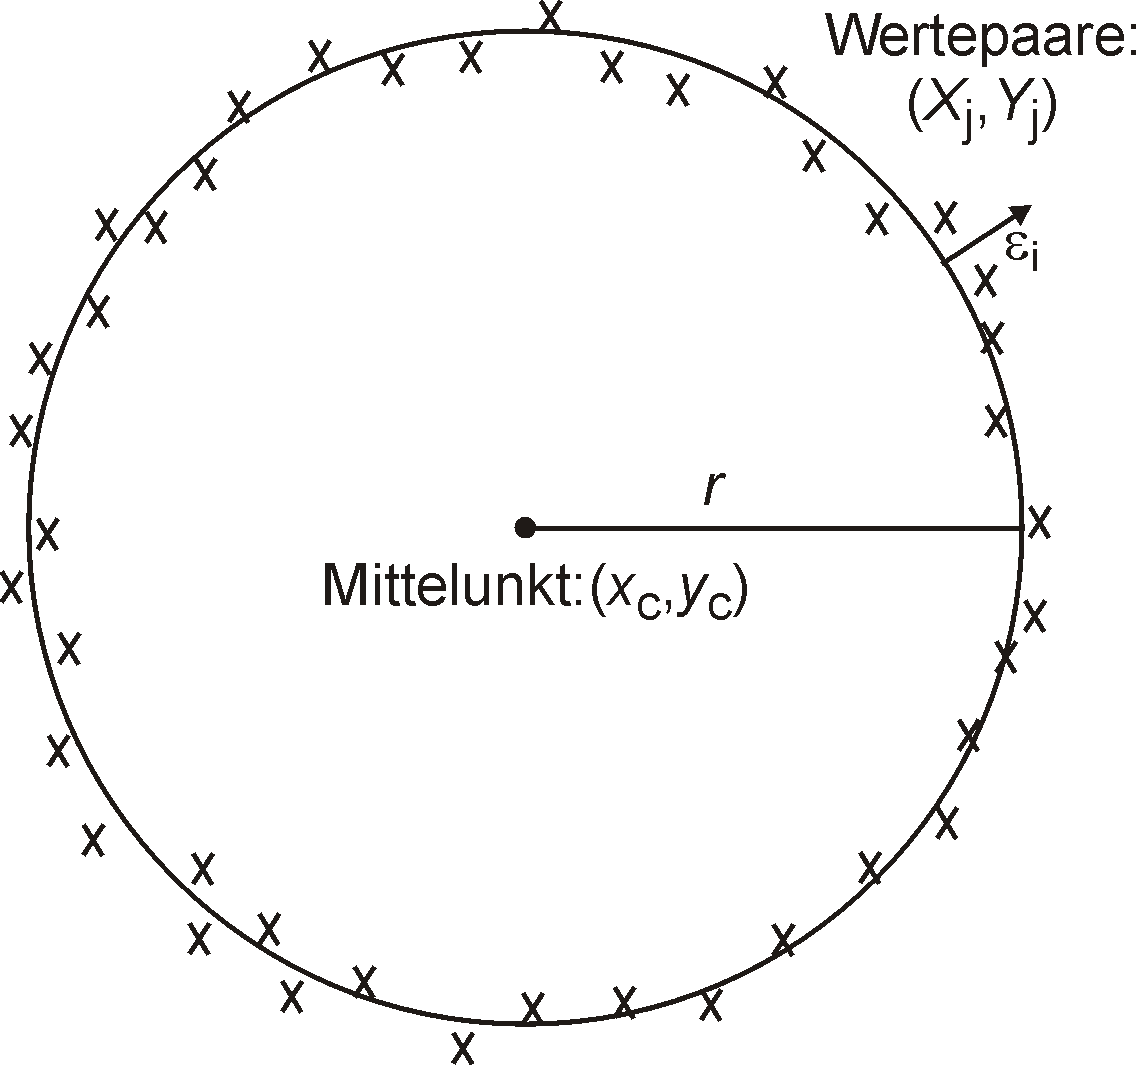
\includegraphics[width=100mm]{03_vorlesung/media/KreisfitSkizze.png}
		\caption{Skizze für den Fit eines Kreises}
		\label{fig:KreisfitSkizze}
	\end{center}
\end{figure}
Es besteht also \textbf{kein linearer} Zusammenhang zwischen den Parametern
$\boldsymbol\theta = [x_\mathrm{c},y_\mathrm{c},r]$ und den
Residuen.
Zur Demonstration des Gauß-Newton Algorithmus nehmen wir zur Vereinfachung an, das wir nur den ersten Parameter, also den
x-Wert des Mittelpunktes $x_c$ schätzen. Die beiden anderen
Parameter setzen wir zu $y_c=0$ und $r=1$.
Dann besteht die Jakobi-Matrix nur aus einer partiellen Ableitung nach dem x-Wert des Mittelpunktes $x_c$. Wenn alle drei Parameter geschätzt werden sollen, müssten entsprechend die partiellen Ableitungen nach $y_c$ und $r$ mitverwendet werden.

Die Messpunkte erfüllen annäherend die Bedingung in Gl.(\ref{eq:Bedingung}):
\[
\sqrt{(X_j-x_\mathrm{c})^2+(Y_j-y_\mathrm{c})^2} \approx r; \quad j=1,\ldots,J
\]

Die Zielfunktion $Q$ lautet dann:
\begin{equation}
	F(x_c) = Q(x_c) := \sum_{j=1}^{J} \left( \sqrt{(X_j-x_\mathrm{c})^2+(Y_j-y_\mathrm{c})^2}-r\right)^2
	\rightarrow \min
\end{equation}
Die partielle Ableitung nach $x_c$ lautet:
\begin{equation}
	DF(x_c) = \frac{\partial Q(x_c)}{\partial x_c} = \D\sum_{j=1}^{J} \left[
	\frac{2(X_j-x_c)\cdot \left( \sqrt{(X_j-x_c)^2 +(Y_j-y_c)^2}-r\right)}
	{\sqrt{(X_j-x_c)^2+(Y_j-y_c)^2}} \right]
\end{equation}
\begin{figure}[!htp]
	\begin{center}
		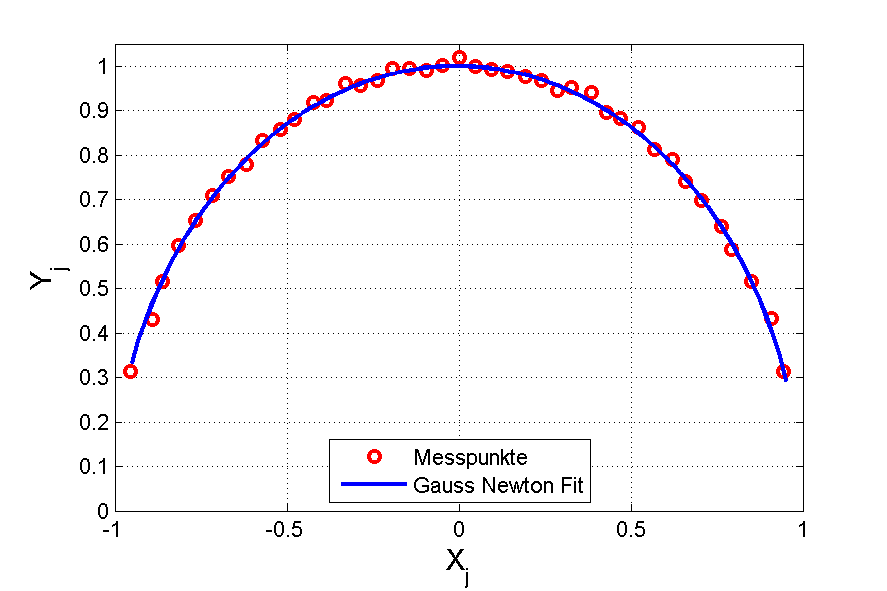
\includegraphics[width=140mm]{03_vorlesung/media/Kreisfit_Gauss_Newton.png}
		\caption{Ergebnis des Gauss Newton Fits}
		\label{fig:Kreisfit_Gauss_Newton}
	\end{center}
\end{figure}
Als Ergebnis erhält man den Halbkreisfit in Abb.~\ref*{fig:Kreisfit_Gauss_Newton} mit einem Schätzwert $x_c$ in dem dargestellten Beispiel von -0.0067.
Das Octave-/Matlab-Skript lautet:
\begin{verbatim}
	% Anzahl der Messpunkte
	M = 41;
	Xj=linspace(-0.95,0.95,M);
	r=1;
	Yj = sqrt(r.^2-Xj.^2);

	figure
	plot(Xj,Yj,'*')

	Xj_Noise = (1-0.01*randn(1,M)).*Xj;
	Yj_Noise = (1-0.01*randn(1,M)).*Yj;

	figure
	plot(Xj_Noise,Yj_Noise,'ro','linewidth',2)
	hold on
	Xj=Xj_Noise;
	Yj=Yj_Noise;
	yc = 0;
	r=1;
	% Suche das Minimum der Funktion F(theta), die xc minimiert
	F = @(theta) sum((sqrt((Xj-theta).^2+(Yj-yc).^2)-r).^2);

	DF = @(theta) sum(2*(sqrt((Xj-theta).^2+(Yj-yc).^2)-r) .*...
	((1/2) * ((Xj-theta).^2 +(Yj-yc).^2).^(-0.5)) .*...
	(2*(Xj-theta)*(-1)));
	% Startparameter
	theta0 = 0.1;
	maxit = 1000; % Anzahl der Interationen
	tol = 1E-15; % Abruchbedingung
	xc_estimate = gauss_newton(F,DF,theta0,maxit,tol);
	disp(xc_estimate);

	Xjfit=linspace(-0.95,0.95,101);
	%
	Yjfit = sqrt(r.^2-(Xjfit-xc_estimate).^2)+ yc;
	plot(Xjfit,Yjfit,'-','linewidth',2)
	grid on;
	xlim([-1,1])
	ylim([0,1.05])
	legend('Messpunkte','Gauss Newton Fit','Location','South')
	xlabel('X_j','fontsize',14)
	ylabel('Y_j','fontsize',14)
	set(gcf, 'PaperUnits', 'centimeters');
	x_width=15 ;y_width= 10;
	set(gcf, 'PaperPosition', [0 0 x_width y_width]);
	print '-dpng' Kreisfit_Gauss_Newton.png
\end{verbatim}

\newpage
\section{Levenberg-Marquardt-Verfahren}
\begin{figure}[htp]
\begin{center}
\includegraphics[width=0.6\textwidth, angle = 0]{03_vorlesung/media/pltSS_nonlin_leastsquare_sin_zB1signal.pdf}
\end{center}
\caption{Beispiel eines sinusförmigen Signals.\label{LSoptiExampleSinus}}
\end{figure}
\begin{figure}
\begin{center}
\includegraphics[width=0.9\textwidth, angle = 0]{03_vorlesung/media/pltSS_nonlin_leastsquare_sin_zB1RQS.pdf}
\end{center}
\caption{Residuenquadratsumme des Beispielmodells eines sinusförmigen Signals
in drei verschiedenen Perspektiven dargestellt (\textsl{oben} und \textsl{unten links})
 und die Beträge der
Gradienten als Funktion der 2 zu schätzenden Parameter (\textsl{unten rechts}).\label{LSoptiExample1SinusRQS}}
\end{figure}
Um eine sinnvolle Konvergenz zu erzielen, ist eine gute Vorkenntnis, also ein geeignetes
Modellparametertupel $\mathbf{p}_0$ erforderlich, das in einigen Problemstellungen
nur schwerlich, oder gar nicht verfügbar ist. Das bedeutet, dass nicht klar ist, ob
der Gradient dazu führt, dass der Parametervektor in eine Mulde hinab klettert, oder auf
einen Berggipfel oder entlang eines Sattelpunktes spaziert.

Die Numeriker haben Verfahren entwickelt, die auf dieser Grundidee den Gradienten
der Zielfunktion (Summe der Quadrate der Residuen) zu berechnen
basieren, aber ausgereiferter sind hinsichtlich Stabilität und Konvergenz.
Der sog.\ der \textsl{Levenberg-Marquardt}-Algorithmus ist eine solche gradientenbasierte Methode,
die in den Numerikbibliotheken zu Matlab, Gnu-Octave, Python bis hin zu Labview, für nichtlineare
Regression zur Verfügung gestellt wird. Die Grundidee dieser Methode wollen wir im Folgenden skizzieren.
Die Problematik, dass sich der Vektor $\Delta \mathbf{p}_{\kappa}$, den wir im
Folgenden \textsl{Inkrementvektor} nennen, verirrt und auf
einen Berggipfel oder entlang eines Sattelpunktes spaziert, soll anhand eines Beispielsignals
illustriert werden. Das Beispiel ist ein zeitabhängiges Spannungssignal mit sinusförmigem Verlauf,
dem als Störung zum einen ein Signal mit höherer Frequenz und kleinerer Amplitude aufmoduliert ist
und zum anderen ein normalverteiltes weißes Rauschen.
Die Amplitude von $5 \, V$ sei fest vorgegeben, aber die zu schätzenden Modellparameter seien
die Wellenlänge und die Phasenlage des Signals. Abb.~\ref{LSoptiExampleSinus} zeigt das Signal als
schwarze Rauten und in Rot das gesuchte \glqq wahre\grqq ~Signal und als blaue, gestrichelte Kurve
das Signal superponiert mit der höherfrequenten Modulation.

Abb.~\ref{LSoptiExample1SinusRQS} zeigt die Summe der Quadrate der Residuen RQS als
Kostenfunktion in drei verschiedenen Ansichten, die zeigen, dass es eine ausgeprägte Minimumsmulde gibt,
aber ebenso ein ausgeprägtes Maximum und noch kleine Rippeln als Nebenminima und Nebenmaxima.
Das Diagramm unten rechts zeigt die Betragsfunktion des Gradienten mit den vielen Nullstellen.
Hier sehen wir, dass sowohl die Maxima als auch die Minima die Nullstellen bilden.

Der \textsl{Levenberg-Marquardt}-Algorithmus ist ein Gradientenverfahren, bei dem das lineare
Gleichungssystems (\ref{GradientQlinGl3})
durch Einführen eines Dämpfungsterms erweitert wird.

Mit der Gauss-Newton-Methode kann also passieren, dass die Summe der Residuen $Q$, siehe  nicht bei jedem Iterationsschritt kleiner
wird. Wenn jedoch der Richtungsvektor $\Delta \mathbf{p}_{\kappa}$ in die abfallende Richtung
zeigt, so kann auch nur ein Bruchteil $\alpha$ des Richtungsvektors gegangen
werden, solange gilt:
\begin{equation}
Q(\mathbf{p}_{\kappa} + \alpha \cdot \Delta \mathbf{p}_{\kappa}) < Q(\mathbf{p}_{\kappa})
\end{equation}
D.~h., wenn bei der Gauß-Newton Methode Divergenz auftritt, so ist eine
mögliche Verbesserung des Verfahrens, einen Bruchteil $\alpha$ des Richtungsvektors $\Delta\mathbf{p}_{\kappa}$ zu nehmen:
\begin{equation}
\mathbf{p}_{\kappa+1}= \mathbf{p}_{\kappa} + \alpha \cdot \Delta\mathbf{p}_{\kappa}
\end{equation}
In anderen Worten, wenn der Inkrement-Vektor zu lang ist, dann muss man diesen
eben kürzen. Das geht natürlich nur unter der Voraussetzung, dass die Richtung
des Vektors auch die Summe der Residuen weiter verkleinert. Der Bruchteil $\alpha$
liegt zwischen
\[
0 < \alpha < 1
\]
Wenn der optimale Bruchanteil $\alpha$ annähernd Null ist, wird eine alternative Methode zur Behandlung der Divergenz verwendet, der sog. \textbf{Levenberg-Marquardt}
Algorithmus.
Die Normalengleichung wird modifiziert, indem der Inkrementvektor $\mathbf{p}_{\kappa}$ in Richtung des steilsten Abfalls gedreht wird. Der Dämpfungsterm stellt einen Schrittweitenfaktor dar, der den Inkrementvektor
so modifiziert, dass das Optimierungsverfahren besser konvergiert. Dieser
Algorithmus wurde unabhängig voneinander von Levenberg (1944), Girard (1958), Wynne (1959),
Morrison (1960) und Marquardt (1963) vorgeschlagen. In der Literatur wird heutzutage meist vom
Levenberg-Marquardt-Algorithmus gesprochen.

Wir schreiben hier nochmal zusammen das zu minimierende Zielfunktional $Q$ aus Gl.~(\ref{ZielfunktionalGrad}) links
und die in Taylorreihe entwickelten Residuen $\boldsymbol{\varepsilon}(\mathbf{p})$
(Gl.~\ref{TaylorResi3}) auf
$$
Q \; = \; \boldsymbol{\varepsilon}(\mathbf{p})^\mathsf{T} \, \boldsymbol{\varepsilon}(\mathbf{p})
\qquad
\boldsymbol{\varepsilon}(\mathbf{p})
\; = \;
\boldsymbol{\varepsilon}(\mathbf{p}_\kappa)
\; + \; \boldsymbol{J}^{(\kappa)} \Delta \mathbf{p}
$$
und setzen diese ineinander ein, so dass die Kostenfunktion wie folgt aussieht
\begin{equation}
Q \; = \; \left( \boldsymbol{\varepsilon}(\mathbf{p}_\kappa)
\; + \; \boldsymbol{J}^{(\kappa)} \Delta \mathbf{p} \right)^\mathsf{T} \,
\left( \boldsymbol{\varepsilon}(\mathbf{p}_\kappa)
\; + \; \boldsymbol{J}^{(\kappa)} \Delta \mathbf{p} \right) .
\label{ZielfunktionalTaylorResi}
\end{equation}
Damit hatten wir im vorigen Abschnitt einen Ansatz erhalten, der
ein bezüglich des Inkrementvektors $\Delta \mathbf{p}_\kappa$ lineares Gleichungssystem
geliefert hatte. Wir notieren Gl.~(\ref{GradientQlinGl3}) hier noch einmal
\begin{equation*}
 \boldsymbol{J}^{(\kappa) \textsf{T}} \, \boldsymbol{J}^{(\kappa)} \, \Delta \mathbf{p}_\kappa
\; \overset{!}{=} \;
-  \boldsymbol{J}^{(\kappa) \textsf{T}} \, \boldsymbol{\varepsilon}(\mathbf{p}_\kappa) .
\end{equation*}

Nun modifizieren wir das Gleichungssystem durch Hinzufügen eines Dämpfungsterms
wie folgt
\begin{equation}
\left(
\boldsymbol{J}^{(\kappa) \textsf{T}} \, \boldsymbol{J}^{(\kappa)}
 + \mu \, \mathrm{diag}\left(\boldsymbol{J}^{(\kappa) \textsf{T}} \, \boldsymbol{J}^{(\kappa)}\right)
 \right) \Delta \mathbf{p}_\kappa \;
\overset{!}{=} \; - \boldsymbol{J}^{(\kappa)^\textsf{T}} \, \boldsymbol{\varepsilon}(\mathbf{p}_\kappa)
\label{ZielfunktionalGradTaylorResiDaempf}
\end{equation}
wobei $\mathrm{diag}\left(\boldsymbol{J}^{(\kappa) \textsf{T}} \, \boldsymbol{J}^{(\kappa)}\right)$
eine Diagonalmatrix ist, die aus den Matrixelementen auf der Hauptdiagonalen von
$\boldsymbol{J}^{(\kappa) \textsf{T}} \, \boldsymbol{J}^{(\kappa)}$ besteht und die
Nebendiagonalelemente alle mit Null besetzt hat.

Der Parameter $\mu$ wird Dämpfungsparameter oder \textsl{Marquardtparameter} genannt.
Die Dämpf\-ungs\-strategie besteht darin, dass für große Werte von $\mu$ die Länge
$\sqrt{\Delta \mathbf{p}_\kappa^\mathsf{T} \, \Delta \mathbf{p}_\kappa}$
der Inkrementschritte $\Delta \mathbf{p}_\kappa$ entsprechend verringert wird.

Diese Methode, die  Länge des Inkrementvektors
$\Delta \mathbf{p}_\kappa$ zu verbessern, also die Werte für den
Dämpf\-ungs\-parameter $\mu$ zu wählen, ist heuristisch.
Es gibt eine Vielzahl von Methoden und Möglichkeiten und wir gucken uns
eine davon an, um einen Einblick zu erhalten, wie soetwas aussehen kann.

Es wird eine Prüfgröße $\rho_{\mu}$ definiert, bei der die Differenz der
Kostenfunktion $Q$ für unterschiedliche Modellparametertupel
verglichen wird mit der Differenz der die Kostenfunktion an der Nachfolgerstelle
zu dem entsprechenden Punkt auf der approximierenden Tangentialebenen
\begin{equation}
\rho_{\mu} :=\frac{Q(\mathbf{p}_\kappa) -
Q(\mathbf{p}_\kappa + \Delta \mathbf{p}_\kappa)}
{Q(\mathbf{p}_\kappa) -
\left( \boldsymbol \varepsilon (\mathbf{p}_\kappa)
    + \mathbf{J}^{(\kappa)} \Delta \mathbf{p}_\kappa \right)^\mathsf{T}
\left( \boldsymbol \varepsilon (\mathbf{p}_\kappa)
    + \mathbf{J}^{(\kappa)} \Delta \mathbf{p}_\kappa \right)  }
=:  \frac{\Delta R(\mathbf{p}_\kappa, \Delta \mathbf{p}_\kappa)}{\Delta \tilde{R}(\mathbf{p}_\kappa, \Delta \mathbf{p}_\kappa)} .
\label{DaempfTuning}
\end{equation}
Die Prüfgröße $\rho_{\mu}$ ist das Verhältnis
\begin{itemize}
\item der Differenz $\Delta R$ des Zielfunktionals $Q$ zwischen
der Vorgängerposition $\mathbf{p}_\kappa$ und $Q$ an der Nachfolgerposition
$\mathbf{p}_\kappa + \Delta \mathbf{p}_\kappa$
des Parametervektors
\item relativ zu der Differenz $\Delta \tilde{R}$ zwischen dem $Q$ an der
Stelle der Vorgängerposition $\mathbf{p}_\kappa$ und dem Wert der Residuenquadratsumme
an der Position auf der Tangentialfläche die an der
Stelle $\mathbf{p}_\kappa$ an die Kostenfunktion $Q$ angelegt wird,
\end{itemize}
um dort das Zielfunktional zu approximieren.

Jetzt wird noch eine Vergleichsgröße, ein Schwellwert gebraucht, mit der die
Prüfgröße verglichen wird, oder auch mehrere Schwellwerte. Hier stellen wir
eine Methode vor, bei der zwei Schwellwerte $\beta_0, \beta_1$ als
Ent\-scheid\-ungs\-grund\-lage für die Wahl des
Wertes $\mu$ verwendet werden, um den Inkrementvektor geeignet zu manipulieren.
Für diese beiden heuristischen Schwell\-wert\-para\-meter $\beta_0$, $\beta_1$
können wir beispielsweise die Werte $\beta_0 = 0.2$, $\beta_1 = 0.8$ wählen.

Tabelle 1: Entscheidungen zur Behandlung des Marquadtparameters

\begin{tabular}{ll}
\hline\hline
$\rho_{\mu} \le \beta_0 $: &
$\Delta \mathbf{p}_\kappa$ wird nicht akzeptiert \textsl{Gewährleistung der Konvergenz} \\
 & $\mu$ wird vergrößert, z.B.\ durch Verdoppeln  $\mu \rightarrow 2 \mu$,\\
 & und die neue zugehörige Korrektur $\Delta \mathbf{p}_\kappa$ wird berechnet\\
\hline
$\beta_0 < \rho_{\mu} < \beta_1$: & $\Delta \mathbf{p}_\kappa$ wird akzeptiert \\
 & bei der Berechnung von $\Delta \mathbf{p}_{\kappa+1}$
  wird als Anfangswert dasselbe $\mu$ gewählt \\
\hline
$\rho_{\mu} \ge \beta_1$: & $\Delta \mathbf{p}_\kappa$ wird akzeptiert \textsl{Effektivität}\\
 & bei der Berechnung  von $\Delta \mathbf{p}_\kappa$ wird \\
 & als Anfangswert ein kleinerer Wert für $\mu$ gewählt, z.B.\ durch Halbieren $\mu / 2$ \\
\hline\hline
\end{tabular}

\newpage
\textbf{Ein möglicher Algorithmus des Levenberg-Marquardt-Verfahrens} \\
Input: Startwert $\mathbf{p}_0$, Zielfunktion $\varepsilon(\mathbf{p}_{\kappa})$, Partielle Ableitungen $J=\varepsilon'(\mathbf{p}_{\kappa})$, Marquardt-Parameter $\mu$, weitere Parameter $0 < \beta_0 < \beta_1 < 1$  \\
\hspace*{1em} \textit{for} $k = 0,1, \ldots$
\begin{itemize}
	\item[i)] Berechne $\varepsilon(\mathbf{p}_{\kappa})$, $F'(\mathbf{p}_{\kappa})$
	\item[ii)] Bestimme den Korrekturvekor $\Delta \mathbf{p}_\kappa$
	\item[iii)] Test, ob die Korrektur $\Delta \mathbf{p}_\kappa$  akzeptabel ist: \\
	$\bullet$ $\rho_{\mu} \le \beta_0: \;$ Setze $\mu = 2 \mu $ und berechne $ \Delta \mathbf{p}_\kappa$ gemäß ii) neu \\
	$\bullet$  $\rho_{\mu} \ge \beta_1: \;$ Setze $\mu = \mu / 2 $ und behalte
	$\Delta \mathbf{p}_\kappa$
	\item[iv)] Setze $\mathbf{p}_{\kappa +1} = \mathbf{p}_\kappa +  \Delta \mathbf{p}_\kappa $
\end{itemize}
\hspace*{1em} \textit{end} \\

Diese Methode wird nun auf das zuvor beschriebene Beispiel des in Abb.~\ref{LSoptiExampleSinus}
dargestellten sinusförmigen Signals mit einem Gnu-Octave/Matlab-Skript getestet.
Ziel ist es, durch die gegebenen Spannungswerte $(s_j,t_j)$ eine Sinusfunktion
durchzulegen. Der Modellansatz für dieses Beispiel lautet:
\begin{equation}
	s(t) \; = \; a \sin(2\pi \frac{t}{\lambda} + \varphi) \; + \; \varepsilon \qquad
	\textrm{mit} \qquad \varepsilon \sim {\cal N}(0,\sigma)
\end{equation}
bei dem die Residuen in Richtung von $s$ streuen und bei dem die Abtastpunkte
entlang der Zeitachse $t$ als Regressor vorgegeben sind, so dass
wir einen Regressionsansatz der Gestalt
\begin{equation}
	\varepsilon_j \; = \; Y_j \; - \; f(X_j, \boldsymbol{p}) \qquad \textrm{mit} \qquad
	j=1, 2,\dots, J
\end{equation}
vorliegen haben. $\boldsymbol{p}$ sind die gesuchten Modellparameter. Die Kostenfunktion sieht damit wie folgt aus
\begin{equation}
	Q(\boldsymbol{p}) \; = \; \sum\limits_{j=1}^J \left(Y_j \; - \; f(X_j, \boldsymbol{p})\right)^2.
\end{equation}
In dem vorliegenden Fall haben wir zwei Modellparameter $p(1) = \lambda$ und $p(2) = \varphi$
\begin{equation}
\boldsymbol{p} =
\left(\begin{array}{c}
	p(1) \\
	p(2)
\end{array}\right)
= \left(\begin{array}{c}
	\lambda \\
	\varphi
\end{array}\right)
\end{equation}
Die Residuen sind wie folgt gegeben:
\begin{equation}
\varepsilon_j = s_j - a \cdot \sin \left[ \frac{2 \pi}{p(1)}t_j +p(2)\right]
\end{equation}
Für die Jakobimatrix benötigen wir die beiden partiellen Ableitungen nach den Modellparametern
$p(1)$ und $p(2)$:
\begin{equation} \boldsymbol{J} =
	\left(	\begin{array}{c} J_{11} \\ J_{21} \end{array}
	\right)
	= \left(
	\begin{array}{c}
		\frac{\D \partial \varepsilon}{\D \partial p(1)} \\
		\frac{\D \partial \varepsilon}{\D \partial p(2)}
	\end{array}
\right)
\end{equation}

\begin{eqnarray}
 \nonumber J_{11} = \frac{\partial\varphi(\boldsymbol{p})}{\partial p(1)} &=&
	- a\cdot \cos \left[ \frac{2\pi}{p(1)} \cdot t +p(2) \right] \cdot
	\left(\frac{-2\pi t}{p(1)^2} \right) \\
	&=& \frac{4a\cdot \pi}{p(1)^2}\cdot t \cdot \cos \left[\frac{2 \pi}{p(1)} t +p(2) \right]
	\label{eq:JakobiMatrix_J11}
\end{eqnarray}
\begin{equation}
	J_{21} = \frac{\partial\varphi(\boldsymbol{p})}{\partial p(2)} = - a \cos \left[
	\frac{2 \pi}{p(1)} t + p(2) \right]
		\label{eq:JakobiMatrix_J21}
\end{equation}

 Das Octave/Matlab-Skript sieht wir folgt aus:

\begin{verbatim}
function fit_sin_LMAC(gen_new)
% Stand: 191105
% Läuft unter Matlab und Octave
t = [0:99]'; % Sekunden
N = length(t);
a = 5; % Volt
lam = 30; % Sekunden
sigma = 0.13*a;
phi = 0.2*pi;
%
am = 0.3*a;
phim = 0.7*pi;
lamm = 0.3*lam;
%
st = a*sin(2*pi*t/lam + phi);
if gen_new
smod = st + am*sin(2*pi*t/lamm + phim);
s = smod + sigma*0.5*randn(1,N)';
save('pltSS_nonlin_leastsquare_sin_zB2.mat','t','s','sigma','a');
else
load('pltSS_nonlin_leastsquare_sin_zB2.mat');
end
%
% Startwerte geraten
%
p0 = [33; 0.23*pi];
x = [t(:) s(:)];
%
% Residuen, muessen als Spaltenvektor vorliegen
%
epsi = @(x, p) (x(:,2) - a*sin(2*pi*x(:,1)/p(1) + p(2)));
%
% partielle Ableitungen der Residuen epsi
% muss M Spalten und J Zeilen haben, wobei M die Anzahl der Fitparameter
% und J die Anzahl der Messpunkte ist
%
\end{verbatim}
siehe Gl.(\ref{eq:JakobiMatrix_J11}) und (\ref{eq:JakobiMatrix_J21})
\begin{verbatim}
Jac = @(x, p) [(4*a*pi/p(1)^2)*x(:,1).*cos(2*pi*x(:,1)/p(1)+p(2)),...
-a*cos(2*pi*x(:,1)/p(1)+p(2))];
%
maxit = 5000; % Anzahl der Iterationen
tol = 1E-15; % Abbruchbedingung
beta0 = 0.2;
beta1 = 0.8;
%
% Startwert des Marquardtparameters
%
mu0 = 10;
%
% Optimierungsrechnung
%
p1=levenberg_marquardt(epsi,Jac,x,p0,mu0,beta0,beta1,maxit,tol);
%
% Ergebnisausgabe
%
disp(['gefittete Werte: lambda = ', ...
num2str(p1(1)),'; phi/pi =   ',num2str(p1(2)/pi)]);

sf = @(x, p) a*sin(2*pi*x/p(1) + p(2));
figure(1);
plot( t, s,'MarkerFaceColor',[0 0 1],'MarkerSize',8, ...
'Marker','diamond','LineStyle','none')
hold on;
plot(t, st, 'g-', 'linewidth', 3)
plot(t, sf(t,p0), 'b-', 'linewidth', 2);
plot(t, sf(t,p1), 'r--', 'linewidth', 2);
legend('Messwerte','Sollfunktion','Startwerte','Fit' )

xlabel('t / s','fontsize', 14);
ylabel('s / V','fontsize', 14);
set(gca,'fontsize',12);
grid on;
print('-dpng','pltSS_nonlin_leastsquare_sin_zB2.png');
end
%
function p=levenberg_marquardt(F,DF,x,p0,mu0,beta0,beta1,maxit,tol)
k = 0;
mu= mu0;
p = p0;
gradQabs = abbruchkrit(F,DF,x,p);
sflag = 1;

while (gradQabs>tol) && (k<maxit) && (mu>tol) && (sflag<2)
[s,mu,sflag] = korrektur(F,DF,x,p,mu,beta0,beta1,tol);
if sflag==1
p=p+s;
end
gradQabs = abbruchkrit(F,DF,x,p);
k=k+1;
end
disp(['Anzahl Interationen: ', num2str(k)]);
end
%
function [s,mu,sflag] = korrektur(F,DF,x,p,mu,beta0,beta1,tol)
s = Delta_p(F,DF,x,p,mu);
Q = F(x,p)'*F(x,p);
DR = Q - F(x,p+s)'*F(x,p+s);
DRtilde = Q - (F(x,p)+DF(x,p)*s)'*(F(x,p)+DF(x,p)*s);
sflag = 1;
if DRtilde > tol
if DR <= beta0*DRtilde
sflag = 0;
mu = 2*mu;
elseif DR >= beta1*DRtilde
mu = mu/2;
end
else
sflag = 2;
end
end
%
function s = Delta_p(F,DF,x,p,mu)
JTJ = DF(x,p)'*DF(x,p);
s = -(JTJ + mu*diag(diag(JTJ)))\(DF(x,p)'*F(x,p));
end
%
function gradQabs = abbruchkrit(F,DF,x,p)
gradQabs = ( F(x,p)'*DF(x,p) * DF(x,p)'*F(x,p) );
end
\end{verbatim}

Dieses Gnu-Octave-/Matlab-Skript hat dazu das in Abb.~\ref{LSoptiExampleSinusFitted} dargestellte Ergebnis mit den Werten
\begin{verbatim}
Anzahl Interationen: 1878
gefittete Werte: lambda = 30.0505; phi/pi = 0.2051
\end{verbatim}
geliefert.
\begin{figure}
\begin{center}
\includegraphics[width=0.8\textwidth, angle = 0]{03_vorlesung/media/pltSS_nonlin_leastsquare_sin_zB2.png}
\end{center}
\caption{Beispiel eines sinusförmigen Signals mit Levenberg-Marquadt-Fit gemäß
Gln.~(\ref{ZielfunktionalGradTaylorResiDaempf}) und (\ref{DaempfTuning}) zusammen mit
den Entscheidungen aus Tabelle 1.\label{LSoptiExampleSinusFitted}}
\end{figure}


Für die nichtlineare Regression gibt es in Gnu-Octave  beispielsweise folgende
Funktion:
\begin{verbatim}
[f, p, cvg, iter] =leasqr (x, y, init, F);
\end{verbatim}
Angewendet auf unser Beispiel vom sinusförmigen Signal kann sie in folgender Weise
verwendet werden
\begin{verbatim}
function fit_sin(gen_new)
 % Stand: 191105
 % Läuft nur unter Octave, da leasqr nur unter Octave
 % frei zur Verfügung steht. Bei Matlab gibt es
 % einen ähnlichen Befehl, der heisst nlinfit
  load('pltSS_nonlin_leastsquare_sin_zB2.mat');
  p0 = [34; 0.23*pi];
  sf = @(x, p) a*sin(2*pi*x/p(1) + p(2));
  [f1, p1, kvg1, iter1, corp1, covp1, covr1, stdresid1, Z1, r21] = ...
  leasqr (t(:), s(:), p0, sf);
  fprintf(stdout,'gefittete Werte: lambda = %1.2f;  phi/pi = %1.2f\n', ...
  p1(1), p1(2)/pi );
  t = [0:99]'; % Sekunden
  N = length(t);
  %
  a = 5; % Volt
  lam = 30; % Sekunden
  sigma = 0.13*a;
  phi = 0.2*pi;
 %
  am = 0.3*a;
  phim = 0.7*pi;
  lamm = 0.3*lam;
 %
  st = a*sin(2*pi*t/lam + phi);
  figure(1);
  plot( t, s, 'kd', ...
  t, st, 'g-.;soll;', ...
  t, sf(t,p0), 'b--;Startwerte;', ...
  t, sf(t,p1), 'r-;gefittet;');
  xlabel('t / s','fontsize', 14);
  ylabel('s / V','fontsize', 14);
  set(gca,'fontsize',12);
  grid on;
  end
\end{verbatim}
und wir erhalten folgendes Ergebnis
\begin{verbatim}
gefittete Werte: lambda = 30.0505;  phi/pi = 0.2051
\end{verbatim}

\newpage
\section{Matlabfunktionen zur Berechnung nichtlinearer Fits}
Es gibt eine Vielzahl an Matlab-Bibliotheksfunktionen, die nichtlineare Optimierungsverfahren implementiert haben. Der Levenberg-Marquardt-Algorithmus ist in Matlab in der Funktion \textsf{lsqnonlin(fun,x0,lb,ub, options)} mit
\textsf{options.Algorithm = 'levenberg-marquardt'} implementiert.
% siee evtl auch mal das Beispiel:
% https://octave.sourceforge.io/optim/function/lsqnonlin.html
Für unser Beispiel mit dem Sinusfit verwenden wir beispielhaft die Funktion \textsf{fminsearch(fun,x0,options)}, in der die Simplexmethode nach Nelder und Mead implementiert ist. Es muss ein Schätzwert
für den Startwert \textrm{x0} angegeben werden. Als \glq OPTIONS\grq~können u.a. gewählt werden TolX (Toleranz, wann abgebrochen werden soll) oder MaxIter (Maximale Anzahl an Iterationen, die durchgeführt werden sollen).
Die zu minimierende Kostenfunktion $Q$ ist für unser Beispiel mit dem Sinusfit gegeben durch:
\begin{equation}
Q(\boldsymbol{p}) = \sum_{j=1}^{J} (a \cdot \sin(2\cdot \pi \cdot t(j) /p(1) + p(2))-s(j))^2
\;\rightarrow \;\textrm{Min.}
\end{equation}
Der dazugehörige Matlab-Code lautet:
\begin{verbatim}
load('pltSS_nonlin_leastsquare_sin_zB2.mat');
a = 5; % Volt
p0 = [34; 0.23*pi];
% Ziel-/ Kostenfunktion:
Q = @(p) sum((a*sin(2*pi*t/p(1) + p(2))-s).^2) ;
tol = 1E-15;
maxit =1000;
p1= fminsearch(Q, p0, optimset('TolX',tol, 'MaxIter', maxit));
disp(['gefittete Werte: lambda =', num2str(p1(1)),';  ', ...
num2str(p1(2)/pi)])
\end{verbatim}
Als Ergebnis erhält man:
\begin{verbatim}
gefittete Werte: lambda =30.0505; phi/pi=0.2051
\end{verbatim}
\begin{figure}[htb]
	\begin{center}
		\includegraphics[width=0.9\textwidth, angle = 0]{03_vorlesung/media/OptimToolMatlab.png}
	\end{center}
	\caption{Optimtool von Matlab: Ergebnis $p(1)=30,05$ und $p(2)=0,644$} \label{fig:Optimtool_von_Matlab}
\end{figure}

\newpage
Tabelle \ref*{tab:Optimierungsverfahren} gibt einen Überblick über
Matlabfunktionen bei Optimierungsproblemen, siehe dazu auch
S.~S.~Rao \cite{Rao09}. $\mathbf{lb}$ steht für \glq lower bound\grq~ und $\mathbf{ub}$ steht für \glq upper bound\grq~

\begin{table}[!ht]
	\caption{Optimierungsverfahren mit Matlab}
	\centering
	\begin{tabular}{p{5cm} | >{\centering\arraybackslash} p{6cm} | p{4cm}}  \hline
		Typ des Optimierungs- \newline problem &  Standardform für die Lösung unter Matlab/Octave &  Matlab/Octave Funktion um das Problem zu lösen \\[1ex]
		\hline \hline
		Funktion von einer  \newline Variablen  & Finde $x$, indem $f(x)$ minimiert wird mit
		$x_1 < x < x_2$ & \textsf{fminbnd} \\[1ex] \hline
		Minimierung ohne Randbedingung von einer Funktion oder mehreren Variablen &
		Finde $\mathbf x$, so dass $f(\mathbf x)$ minimiert wird.
		Hinweis: Simplexmethode nach Nelder und Mead &
		\textsf{fminunc} oder \newline \textsf{fminsearch} \\[1ex] \hline
		Lineares Problem & Finde $\mathbf x $ durch Minimierung von $\mathbf{f^T x}$ mit $A \mathbf x \le b$, $A_{eq} \mathbf x = \mathbf b_{eq}$, \newline
		$\mathbf{lb} \le \mathbf{x} \le \mathbf{ub}$ & \textsf{linprog} \\[1ex] \hline
		Quadratisches Problem & Finde $\mathbf x $ durch Minimierung von $\frac{1}{2} \mathbf{x^T}\mathbf{f^T x}$ mit $A \mathbf x \le \mathbf b$,
		\newline $A_{eq}$ $\mathbf x = \mathbf b_{eq}$, \newline
		$\mathbf{lb} \le \mathbf{x} \le \mathbf{ub}$ & \textsf{quadprog} \\[1ex] \hline
		Minimierung von Funktionen von mehreren Variablen mit Nebenbedingungen &
		Finde $\mathbf x $ durch Minimierung von $\frac{1}{2} \mathbf{x^T}\mathbf{f^T x}$ mit $\mathbf{c(x) \le 0}$,
		$\mathbf{c_{eq} = 0}$ \newline
		$A \mathbf x \le \mathbf b$,
		$A_{eq}$ $\mathbf x = \mathbf b_{eq}$, \newline
		$\mathbf{lb} \le \mathbf x \le \mathbf{ub}$ & \textsf{fmincon} \\[1ex] \hline
		Minimax Problem & Finde das  $\mathbf x $ welches die Maxima
		von mehreren gegeben Funktionen $F_i(\mathbf x)$ minimiert,
		so dass  $\mathbf{c(x) \le 0}$,
		$\mathbf{c_{eq} = 0}$ \newline
		$A \mathbf x \le \mathbf b$,
		$A_{eq}$ $\mathbf x = \mathbf b_{eq}$, \newline
		$\mathbf{lb} \le \mathbf x \le \mathbf{ub}$ & \textsf{fminimax} \\[1ex] \hline
	\end{tabular}
	\label{tab:Optimierungsverfahren}
\end{table}

Bei Matlab gibt es die in Abb. \ref{fig:Optimtool_von_Matlab} gezeigte graphische Oberfläche, das sog.
\glq Optimization tool\grq~(Funktionsaufruf: \glq optimtool\grq),
die die in Tab. \ref*{tab:Optimierungsverfahren} aufgeführten
Optimierungsverfahren und noch einige mehr zur Verfügung stellt.
Dieses Tool eignet sich ganz gut, wenn man sich einen ersten Überblick
über die in Matlab implementierten Optimierungsverfahren verschaffen will. \\

\newpage
\section{Gradientenverfahren mit unterschiedlichen Varianzen}
\label{unterschiedVar}
Die Varianzen (und Kovarianzen) der Residuen sind immer auch Funktion der Modellparameter. Als wir die
Maximum-Likelihood-Methode eingeführt haben, hatten wir sie ausgeklammert und bei der Bestimmung
des Minimums über die Summer der kleinsten Residuenquadrate weggekürzt. Sie
lassen sich für den Fall ausklammern, bei dem die Streuung bezüglich des Modells
für alle Messpunkte gleich ist, also
\begin{equation}
Q(\mathbf{p}) \; = \;
 \frac{\boldsymbol{\varepsilon}(\mathbf{p})^\mathsf{T} \, \boldsymbol{\varepsilon}(\mathbf{p})}{\sigma^2(\mathbf{p}))}
\end{equation}
und
\begin{equation}
\nabla_{\mathbf{p}} Q(\mathbf{p})  \; = \;
\frac{2}{\sigma^2(\mathbf{p})} \boldsymbol{\varepsilon}^\textsf{T}(\mathbf{p})
 \, \boldsymbol{J} \overset{!}{=} \; \left(\begin{array}{ccc} 0 & \dots & 0 \end{array}\right)
\label{ZielfunktionalGradJmitSigma}
\end{equation}
was einfach mit $\frac{\sigma^2(\mathbf{p})}{2}$ multipliziert werden kann, so dass wir mit
den Residuen wie oben beschreiben weiter arbeiten können, indem wir diese in Taylorreihe entwickeln.

Für den Fall, dass es unterschiedliche Varianzen für Residuen der verschiedenen Beobachtungstupel
$(X_{1,j},\dots,X_{N,j})$ gibt, ordnen wir $\sqrt{\sigma_j^2} = \sigma_j$
den Residuen zu mit
\begin{equation}
Q(\mathbf{p}) \; = \;
  \left(\begin{array}{ccc}
  \frac{\varepsilon_1(\mathbf{p})}{\sigma_1(\mathbf{p})} & \dots &
 \frac{\varepsilon_J(\mathbf{p})}{\sigma_J(\mathbf{p})} \end{array} \right)
\, \left(\begin{array}{c} \frac{\varepsilon_1(\mathbf{p})}{\sigma_1(\mathbf{p})}\\
 \vdots\\ \frac{\varepsilon_J(\mathbf{p})}{\sigma_J(\mathbf{p})}\end{array} \right)
\label{ZielfunktionalJmitW}
\end{equation}
d.h.\ kurz ohne jedesmal das \glqq Funktion von $\mathbf{p}$\grqq oder
\glqq abhängig von $\mathbf{p}$\grqq, also $(\mathbf{p})$,
mitzuschreiben
\begin{equation}
Q(\mathbf{p}) \; = \;
  \boldsymbol{\varepsilon}^\textsf{T}
\, \left(\begin{array}{cccc} \frac{1}{\sigma_1^2} & \dots & & 0 \\
  & \ddots & \\
 0 & & \dots &  \frac{1}{\sigma_J^2} \end{array} \right) \, \boldsymbol{\varepsilon}
\label{ZielfunktionalJmitW1}
\end{equation}
Je stärker eine Beobachtung $j$ abweicht, also je größer die Varianz $\sigma_j^2$,
desto geringer fällt der Summand $\frac{\varepsilon_j^2}{\sigma_j^2}$ in der Kostenfunktion $Q$
ins Gewicht, weshalb man diese auch als Gewichte $w_j = \frac{1}{\sigma_j^2}$ bezeichnet
und die Matrix als Gewichtsmatrix $\mathbf{W}$ also
\begin{equation}
Q(\mathbf{p}) \; = \;
  \boldsymbol{\varepsilon}^\textsf{T}
\, \mathbf{W} \, \boldsymbol{\varepsilon}
\label{ZielfunktionalJmitW2}
\end{equation}
und mit
\begin{equation}
\frac{1}{2} \nabla_{\mathbf{p}} Q(\mathbf{p})  \; = \; \boldsymbol{\varepsilon}^\textsf{T}(\mathbf{p})
 \, \mathbf{W} \, \boldsymbol{J}
\label{ZielfunktionalGradJW}
\end{equation}
sieht unser Optimierungsproblem wie folgt aus
\begin{equation}
\lim_{\mathbf{p} \rightarrow \mathbf{\hat p}}
\boldsymbol{\varepsilon}^\textsf{T}(\mathbf{p})
 \, \mathbf{W}(\mathbf{p}) \, \boldsymbol{J}(\mathbf{p})
 \; = \; \left(\begin{array}{ccc} 0 & \dots & 0 \end{array}\right) .
\label{ZielfunktionalGrad1W}
\end{equation}
Die Gleichungen (\ref{GradientQlinGl3}) und (\ref{ZielfunktionalGradTaylorResiDaempf})
werden damit zu
\begin{equation}
 \boldsymbol{J}^{(\kappa) \textsf{T}} \, \mathbf{W}(\mathbf{p}_\kappa) \,
\boldsymbol{J}^{(\kappa)} \, \Delta \mathbf{p}_\kappa
\; \overset{!}{=} \;
-  \boldsymbol{J}^{(\kappa) \textsf{T}} \, \mathbf{W}(\mathbf{p}_\kappa) \,
\boldsymbol{\varepsilon}(\mathbf{p}_\kappa) .
\label{GradientQlinGl3W}
\end{equation}
und mit Dämpfungs- bzw.\ Marquardtparameter
\begin{equation}
\left(
\boldsymbol{J}^{(\kappa) \textsf{T}} \, \mathbf{W}(\mathbf{p}_\kappa) \, \boldsymbol{J}^{(\kappa)}
 + \mu \, \mathrm{diag}(\boldsymbol{J}^{(\kappa) \textsf{T}} \, \mathbf{W}(\mathbf{p}_\kappa) \, \boldsymbol{J}^{(\kappa)}) \right) \Delta \mathbf{p}_\kappa \;
\overset{!}{=} \; - \boldsymbol{J}^{(\kappa)^\textsf{T}} \,
\mathbf{W}(\mathbf{p}_\kappa) \, \boldsymbol{\varepsilon}(\mathbf{p}_\kappa) .
\label{ZielfunktionalGradTaylorResiDaempfW}
\end{equation}


\section{Robuste Schätzverfahren}
\label{robustEstimation}
Wir haben nun eine Kostenfunktion $Q$ mit Gewichtsfaktoren kennengelernt, Gl.~(\ref{ZielfunktionalJmitW2}),
bei der die Gewichte die Kehrwerte der Varianzen sind $w_j = \frac{1}{\sigma_j^2}$, die sich eigentlich
aus der Abweichung der Beobachtungen vom Modell ergeben. Wenn kein {\`a} priori Wissen über
diese Varianzen vorliegt, aber bekannt ist, dass die Verteilung der
Residuen aller Beobachtungen nicht gauß\-ver\-teilt ist, soll das Problem dennoch mit der
Maximum-Likelihood-Methode gelöst werden. Es kommt vor, dass einzelne Beobachtungen
sehr weit von der Erwartung entfernt sind. Man sagt, dass sie signifikant abweichen. Die Gaußverteilung erlaubt dieses auch, denn sie hat einen Definitionsbereich für die Residuen $\varepsilon$,
der von minus Unendlich bis plus Unendlich geht, ihre Ausläufer auch \textsl{Tails} genannt,
sind unbegrenzt. Die Wahrscheinlichkeit ist aber sehr gering, kleiner als $5~\%$, dass der Betrag der
Residuen $\varepsilon$ einen Wert annimmt, der größer als
$1.65 \, \sigma$ ist, aber er kann auftreten. Liegen deutlich mehr als $5~\%$
der Beobachtungen außerhalb eines Vertrauensintervalls von beispielsweise $[-3 \sigma, 3 \sigma]$,
dann ist dies ein Indiz dafür sein, dass das Modell unzureichend ist. Es kann sein, dass es auch nicht
um ein vollständigeres Modell geht, sondern darum, nur die zum betrachteten Modell passenden Beobachtungen
berücksichtigen zu wollen. Die übrigen Beobachtungen sollen als Ausreißer, die nicht zum
eigentlichen zu untersuchenden Prozess gehören, nicht an dem \textsl{Least-Square-Fit}
beteiligt werden oder zumindest ihre Beteiligung daran (ihr Gewicht) reduziert wird.

Die Idee für die Realisierung dieser Aufgabe ist, die Verteilung der Residuen durch Umgewichten so zu verändern, das
sie wieder die Gestalt einer Normalverteilung bekommt. Wir führen Gewichtsfaktoren $w = \delta$ ein,
die eine Funktion des Abstands $\varepsilon$ einer Beobachtung vom Modell ist, so dass die Wahrscheinlichkeitsdichte
der Abweichung $\tilde \varepsilon$ einer Normalverteilung folgt. Gesucht ist eine Gewichtsfunktion
$\delta \! : \varepsilon \mapsto \delta(\varepsilon)$ für die gilt
\begin{equation}
\tilde \varepsilon \; = \; \delta(\varepsilon) \; \varepsilon \quad \Rightarrow
\quad \tilde \varepsilon \sim {\cal N}(0,\sigma) .
\end{equation}
Mit Hilfe der Gewichtsfunktion werden aus den Residuen die Gewichtsfaktoren
$w_j = \delta_j = \delta(\varepsilon_j)$ berechnet. Da man die Residuen erst nach
Schätzung der Modellparameter gewinnt, erfordert dies wie bei der nichtlinearen Optimierung
auch sonst, einen iterativen Prozess.

Wir betrachten folgende Kostenfunktion
\begin{equation}
Q(\mathbf{p}) \; = \; \sum_{j=1}^J \, \delta_j \, \varepsilon_j(\mathbf{p})^2 .
\label{robustEstim}
\end{equation}

Zunächst werden die Parameter ungeachtet möglicher Ausreißer mittels \textsl{Least Square}-Methode
ohne Gewichte
\begin{equation}
 \min_{\mathbf{p}} Q(\mathbf{p}) \qquad \mathrm{mit} \qquad
Q(\mathbf{p}) \; = \; \sum_{j=1}^J \, \varepsilon_j(\mathbf{p})^2 .
\label{linEstim}
\end{equation}
geschätzt mit $\mathbf{p}_0$.

Wir betrachten wieder ein einfaches Beispiel, in dem es nur einen Parameter $y$ gibt und eine
Messgröße $X_1$ mit $J$ Beobachtungen $(X_{1,1},\dots,X_{1,J})$.
Dabei wird davon ausgegangen, dass die Beobachtungen zu einer Grundgesamtheit, also zu einem Parameter gehören.
Die Beobachtungswerte werden histogrammiert. Das Histogramm ist in Abb.~\ref{biasExampleKap3} dargestellt.
\begin{figure}
\begin{center}
\includegraphics[width=90mm]{03_vorlesung/media/learn_robust.pdf}
\caption{Beispiel für nicht erwartungsgemäße Beobachtungen}
\label{biasExampleKap3}
\end{center}
\end{figure}
Für das Histogramm werden $K \, = \, 80$ Klassen (engl.\ \textsl{bins}) gewählt, die Anzahl der Beobachtungen umfasst $J \, = \, 2200$.
Die Klassenbreite ist dann
\begin{equation}
\Delta \xi \; = \; \frac{1}{K} \left( \max \left\{X_{1,j}\right\} \; - \; \min \left\{X_{1,j}\right\} \right)
\end{equation}
so dass $K+1$ Klassengrenzen $\xi_{\mathrm{G}, k}$ vorliegen,
deren Indizes wir von Null bis $K$ zählen:
\begin{equation}
 \xi_{\mathrm{G}, k} \; = \; k \, \Delta \xi \; + \; \min \left\{X_{1,j}\right\}
\qquad k = 0, \dots, K
\label{limkthbin}
\end{equation}
und die Mitte in der jeweiligen Klasse für den Wert der Klasse verwenden
\begin{equation}
 \xi_k \; = \; k \, \Delta \xi  \, + \, \frac{1}{2} \Delta \xi  \; + \; \min \left\{X_{1,j}\right\}
\qquad k = 1, \dots, K
\label{kthbin}
\end{equation}
wobei die Anzahl der Klassen $K$ ist.

Die Anzahl der Einzelbeobachtungen, für die gilt
\begin{equation}
\xi_{\mathrm{G}, k-1} \; \leq \; X_{1,j} \; <  \xi_{\mathrm{G}, k},
\end{equation}
nennen wir \textsl{Häufigkeit} $n_k$. Bei der letzten Klasse, also für
$k = K$ wird auch bei der rechten Intervallgrenze ein $\leq$.
Damit ist die diskrete Funktion $n(\xi)$ die Häufigkeitsverteilung.

Der Schätzwert für den Parameter ist nach der Maximum-Likelihood / Least-Square-Methode der
Mittelwert, der hier den Wert $25.47$ annimmt. In Wirklichkeit gehören die Beobachtungswerte gar nicht zu
nur einer Grundgesamtheit, sondern $1750$ gehören zu dem Parameter $\mu_1 \, = \, 23.00$ und $450$ zu $\mu_2 \, = \, 35.00$.
Diese Wirklichkeit kennt aber niemand. Bei Betrachten des Histogramms sieht der Messtechniker jedoch, dass ein
Nebenmaximum vorliegt, es keine reine Gaußverteilung ist. Die weiter entfernt liegenden Beobachtungen sollen unterdrückt werden
durch entsprechende Wahl zugehöriger Gewichtsfaktoren $\delta_j$.

Eine mögliche Wahl für die Gewichtsfaktoren ist die \textsl{Tuckey biweight}-Funktion.
\begin{equation}
\delta_j \; = \;
\left\{ \begin{array}{cl}
\left( 1 \, - \, \left( \frac{X_{1,j} \, - \, y^{(\kappa)}}{c^{(\kappa)}} \right)^2 \right)^2 &
	\mathrm{falls} \; \mid X_{1,j} \, - \, y^{(\kappa)} \mid \, \leq \, c^{(\kappa)} \\
0 & \mathrm{sonst}
\end{array} \right.
\end{equation}
wobei $\kappa$ der Zähler für den Iterationsschritt ist und $c^{(\kappa)}$ ein passend zur Anwendung zu wählender Faktor ist, hier beispielsweise
\begin{equation}
c^{(\kappa)} \; = \; \mathrm{median} \mid X_{1,j} \, - \, y^{(\kappa)} \mid
\end{equation}
Die Kostenfunktion, deren Gewichte von den iterativ bestimmten Residuen und damit von den
iterativ geschätzten Parametern abhängt, stellt ein nichtlineares Optimierungsproblem
$ \min_{\mathbf{p}} Q(\mathbf{p}) $ dar, mit
\begin{equation}
Q(\mathbf{p}) \; = \; \sum_{j=1}^J \; \varepsilon_j^2 \;
\left( 1 \, - \, \left( \frac{\varepsilon_j(\mathbf{p}) }{c(\mathbf{p})} \right)^2 \right)^2 \;
H(\mid \varepsilon_j(\mathbf{p}) \mid - c(\mathbf{p})) \;
H(c(\mathbf{p}) - \mid \varepsilon_j(\mathbf{p}) \mid ),
\label{robustEstim2}
\end{equation}
wobei $H$ für \textsl{Heaviside}- oder Sprungfunktion steht.

\begin{figure}
\begin{center}
\includegraphics[width=100mm]{03_vorlesung/media/learn_robust_2.pdf}
\caption{\label{RobustIter} Umgewichten um die Verteilungform der Normalverteilung anzupassen}
\end{center}
\end{figure}

Der Median von den Absolutbeträgen der Residuen $\varepsilon_j \, = \, X_{1,j} \, - \, y^{(\kappa)}$ wird dadurch gewonnen,
dass man die Werte der Größe nach sortiert und dann den mittleren nimmt, also den, auf dem Platz in der Mitte der sortierten
Anordnung liegt.
Abb.~\ref{RobustIter} stellt die ursprüngliche Häufigkeitsverteilung aus Abb.~\ref{biasExampleKap3} als
durchgezogene, schwarze Linie dar. Nach dem ersten Iterationsschritt der Umgewichtung, hat sich die Verteilung so verändert,
wie es durch die blaue gestrichpunktete Linie gezeigt wird, zu der ein Mittelwert von $24.20$ gehört. Nach mehr als acht Iterationen
wurde ein Mittelwert von $23.23$ erzielt und die mit rot gestrichelter Verteilungskurve eingezeichnet sind.


\chapter{Konzepte der Statistik für die Messdatenanalyse}
\label{konzepteStatistik}
\label{KonzepteinverseProbleme}

\section{Konzepte zum Lösen inverser Probleme}

In den letzen drei Kapiteln (Vorlesungswochen) haben wir einen Einblick in die
Vorgehensweise der Maximum-Likelihood-Methode erhalten:
\begin{enumerate}
\item Die Idee von \textsl{Modell} und \textsl{Lösen inverser Probleme} wurde
  genannt.
\item Zur Lösung inverser Probleme wurde das Schätzen von Parametern, die
 linear in die Modellgleichung eingehen, durch \textsl{lineare Regression} vorgestellt.
\item Ein Einblick in mögliche Verfahren zur Lösung inverser Probleme durch
  Schätzen von Parametern, die nicht-linear in die Modellgleichung eingehen,
  wurde gegeben. Hier wurden kurz drei Verfahren zur \textsl{nicht-linearen Optimierung}
  vorgestellt.
\end{enumerate}
Wir haben dabei gesehen, dass es bei der Messdatenanalyse um die Schätzung von
physikalischen Größen geht, die indirekt über das Messen anderer Größen,
direkter Messgrößen, ermittelt werden.
Die Aufgabe der Messtechnik lässt sich auch beschreiben als die Bestimmung
des Wertes von physikalischen Größen durch Messverfahren, die auf
physikalischen Prinzipien basieren. Die von einem Sensorsystem angezeigten
Größen sind dabei im allgemeinem andere Größen als diejenigen, die zu messen sind.

Wir hatten in der ersten Vorlesung, in Abschnitt \ref{ModelleStatistik},
das Beispiel \glqq Beugung am Gitter\grqq ~betrachtet,
um die Aufgabenstellung zu verstehen, dass man
aus den einem Messsystem direkt zugänglichen Größen die gesuchten physikalischen
Größen gewinnen möchte. Dabei wurde der Begriff des \textsl{Lösens inverser Probleme}
eingeführt. Nachdem wir bereits Methoden zur Ermittlung von indirekten
Messgrößen als Modellparameter kennen gelernt haben, haben wir die Chance uns
unter den Ideen dieses Konzeptes mehr vorstellen zu können.

Darüber hinaus wurde in Abschnitt \ref{ModelleStatistik} schon mal erwähnt, dass
es etwas unterschiedliche Konzepte oder Heransgehensweisen für Schätzverfahren gibt.
Auf der einen Seite steht der sogenannte \textsl{frequentistische} Ansatz, bei dem allein
Beobachtungswerte direkter Größen verwendet werden und die Annahmen über die
Verteilung der Streuung der direkten Größen impliziet schon ins Schätzverfahren
selber eingebaut sind. Der Begriff Frequenz wurde an dieser Stelle aus der
englischen Sprachkonvention \textsl{frequency} übernommen. Das
heißt hier \textsl{Häufigkeit} und nicht \textsl{Frequenz} wie wir das im Deutschen
vielfach mit einer periodischen Bewegung verbunden verstehen. Aber auch die
deutsche Sprache kennt die Sprechweise: \glqq Dies oder jenes Restaurant oder so
wird gut frequentiert\grqq ~im Sinne von \glqq wird häufig besucht\grqq.

Eine Verallgemeinerung der Schätzmethoden wurde in den letzten Jahrzehnten
in die Messdatenanalyse eingeführt, bei der auch die Modellparameter selber als
Zufallsgrößen behandelt werden. Auch ihnen wird eine Streuung, also
Wahrscheinlichkeitsverteilung zugrunde gelegt. Bei diesen Verfahren lassen sich
Schätzwerte und Werte zur Unsicherheit der Modellparameter in die aktuelle
Schätzung mit einbeziehen. Diese verallgemeinerten Methoden, die die Modellparameter
als Zufallsgrößen betrachten, werden \textsl{bayesische} Methoden genannt.

Bevor wir diese beiden Ansätze (frequentistisch und bayesisch) gegenüber
stellen und vergleichen, wollen wir folgende
zwei Blickrichtungen, messtechnische Aufgaben zu betrachten, beleuchten:
\begin{itemize}
\item als Modell von der Physik des Messprinzips gemeinsam mit dem statistischen
Modell, dass die Größen Zufallsgrößen sind,
\item als inverses Problem.
\end{itemize}
Ein Modell wird dargestellt durch eine Vorstellung darüber, wie die
indirekten Messgrößen $Y_m$ mit den direkten Messgrößen $X_i$ verknüpft sind:
\begin{equation}
(Y_1, \dots, Y_M) \xrightarrow{\mathrm{Modell}} (X_1, \dots, X_N)
\label{forwardModel1}
\end{equation}
\begin{figure}
\begin{center}
\includegraphics[width=0.8\textwidth, angle = 0]{04_vorlesung/media/Modell1.pdf}
\end{center}
\caption{Modellbildung zur Gewinnung indirekter Messgrößen aus direkten Messgrößen}
\end{figure}

Ein Messvorgang liefert Beobachtungen zu den direkten Messgrößen.
Die wahren Werte der indirekten Größen bleiben verborgen. Die
indirekten Größen können nur geschätzt werden, oftmals auch nur approximiert werden,
weil die Modelle den physikalischen Sachverhalt nur annähernd beschreiben;
denn die Realität ist deutlich komplexer und wird von vielfältigen Einflussfaktoren
bestimmt. Die approximierenden und zufällig streuenden Größen, die die indirekten Messgrößen
repräsentieren, sind die Modellparameter.
Die Abweichungen der Modellparameter entstehen also zum einen
durch vereinfachende Modellannahmen und zum anderen durch zufällige Einflüsse wie das
thermische Rauschen von Elektronik oder Vibrationen im Laborraum.

Im vorigen Kapitel hatten wir bereits den Bezeichner $\mathbf{p}$ für die Modellparameter
verwendet: $\mathbf{p} = (P_1, \dots, P_M)$.
Der Buchstabe $\mathbf{p}$ steht hier einfach nur für den Anfangbuchstaben
von dem Begriff Parameter und der Fettdruck weist darauf hin, dass es ein Vektor mit vielen
Einzelparametern sein kann und dient ferner dazu, das Symbol von dem für die Wahrscheinlichkeitsdichte
zu unterscheiden. Diese wird mit $p$ für den Anfangsbuchstaben von \textsl{probability} bezeichnet.
Für die einzelnen Parameter $P_m$ verwenden wir hier den Großbuchstaben, um die Unterscheidung zur
Wahrscheinlichkeitsdichtefunktion zu haben, sowie in Anlehnung an die Konvention Großbuchstaben
$X_i$ und $Y_m$ für die Messgrößen zu verwenden.
\begin{equation}
P_1 \approx Y_1, \dots, P_M \approx Y_M
\end{equation}
Der Schätzvorgang wird als \textsl{Lösen eines inversen Problems} interpretiert.
\begin{equation}
(X_1, \dots, X_N) \xrightarrow{\mathrm{inverses \; Problem}} (Y_1, \dots, Y_M)
\label{inverseProblemEq}
\end{equation}

Dazu haben wir die \textsl{Maximum-Likelihood}-Methode kennen gelernt, und gesehen, wie
aus ihr die Methode der kleinsten Residuenquadratsumme hervorgeht. Die Wahrscheinlichkeit,
dass ein Messwert um den Wert $\varepsilon$ von dem geschätzten Modell abweicht, folgt
einer Normalverteilung. Mit anderen Worten kann man auch sagen, dass
die Verteilung der Residuen eine Gaußverteilung ist.
Die Begriffe Gaußverteilung und Normalverteilung verwenden wir synonym.
\begin{equation}
p(\varepsilon | \theta_1,\dots,\theta_M, \sigma) \; = \; \frac{1}{\sigma \sqrt{2 \pi}}
e^{-\frac{1}{2} \left(\frac{\varepsilon}{\sigma}\right)^2}
\label{Maximumlikelihood1}
\end{equation}
Die Symbolik $p(\varepsilon | \theta_1,\dots,\theta_M, \sigma)$ wird gesprochen:
\begin{quote}
Wahrscheinlichkeit $p$ des Eintretens des Ereignises $\varepsilon$
gegeben die Parameter $\theta_1,\dots,\theta_M$ und $\sigma$.
\end{quote}
Der Sprachgebrauch \glqq Eintretens des Ereignisses $\varepsilon$\grqq ~stellt die
Sprechweise der Statistik für \textsl{bedingte Wahrscheinlichkeiten} dar.

\textsl{Bedingte Wahrscheinlichkeit} heißt:
\begin{quote}
Die Wahrscheinlichkeit des Eintretens
zweier Ereignisse $A_1$ und $A_2$ geteilt durch die Wahrscheinlichkeit des Eintretens von $p(A_2)$
\begin{equation}
p(A_1 | A_2) \; = \; \frac{p(A_1 \; \mathrm{und} \; A_2)}{p(A_2)}
\end{equation}
\end{quote}
Zur Illustration des Begriffs der bedingten Wahrscheinlichkeit betrachten wir ein
Kartendeck mit 52 Spielkarten: Die Anzahl der Buben $B$ ist $4$, die Wahscheinlichkeit, einen Buben
zu ziehen, ist $4/52$, die
Wahrscheinlichkeit $p(B | F)$ von allen Bildern bzw.\ Figuren $F = \{B, D, K\}$, einen
 Buben zu ziehen, ist $p(B | F) = 1/3$, die Wahrscheinlichkeit, eine Bildkarte zu ziehen ist $12/52$
$$
p(B | F) = \frac{p(B)}{p(F)} = \frac{4/52}{12/52} = \frac{4}{12} = \frac{1}{3} .
$$

In den angewandten Wissenschaften, Messtechnik,
Elektrotechnik, etc.\ spricht man von der Wahrscheinlichkeit, dass die Messgröße
oder hier die Abweichung der Messgröße vom Modell einen Wert $\varepsilon$ annimmt oder
dass dieser Wert \glqq beobachtet\grqq ~wird unter der Bedingung, dass die Modellparameter
die Werte $\theta_1,\dots,\theta_M, \sigma$ haben.


In Kapitel \ref{KapitellinReg} wurden Sie mit der Regressionsrechnung vertraut gemacht, die
eine spezielle Anwendung der Maximum-Likelihood-Methode darstellt, bei der
Größen beteiligt sind, die keine Zufallsgrößen darstellen, die Regressoren.
Die Residuen und entsprechend die Regressanden sind die Zufallsgrößen,
für die die in Gl.~(\ref{Maximumlikelihood1}) formulierte Wahrscheinlichkeitsdichte
angenommen wird.
Diese Modellannahme, dass die \textsl{Residuen} normalverteilt seien,
hatten wir in Abschnitt \ref{RegressionsIdee} wie folgt formuliert:
\begin{quote}
Die abhängigen Größen $Y$, d.h.\ die \textsl{Regressanden}, streuen und ihre Residuen sind
	normalverteilt mit Erwartungswert $E(\varepsilon) = 0$ und Varianz $\mathrm{Var}(\varepsilon) = \sigma^2$.
	Die Residuen sind \textsl{unabhängig und identisch verteilt}, kurz u.i.v.
	\begin{equation}
	\varepsilon \; \overset{\mathrm{u.i.v.}}{\sim} \; \mathcal{N}(0,\sigma) .
	\end{equation}
\end{quote}
Ein Residuum der linearen Regression mit $Y$ als Regressand und $X_i$ als Regressoren
hat folgende Gestalt
\begin{equation}
\varepsilon_j \; = \; Y_j \; - \; \sum\limits_{i=1}^{M} \theta_i \, X_{i,j}
\end{equation}
wobei der Bezeichner $Y$ der Regressionsrechnung die direkte Messgröße ist und die
Regressoren ebenfalls zu den direkten Größen gehören, jedoch nicht als Zufallsgrößen mit
Streuung, sondern mit vorgegebenen, deterministischen Werten.

Ein Residuum nach der Methode der kleinsten Quadrate für ein Modell mit genau nur einer
einzigen Zufallsgröße $X$ mit einem Modellparameter $\mu$ ist einfach
\begin{equation}
\varepsilon_j \; = \; X_j \, - \, \mu .
\label{oneQuantityOnly1}
\end{equation}

Im Fall der linearen Regression repäsentiert $\mathbf{p} = (\theta_1,\dots,\theta_M)$,
im Fall der Geraden $\mathbf{p} = (\alpha, d)$ und im Fall der Einzelgröße
$\mathbf{p} = \mu$.

Die Schätzung von Modellparametern besteht dann darin, die Modellparameter auszuprobieren,
d.h.\ viele unterschiedliche Werte \glqq auszuprobieren\grqq,
\begin{equation}
(P_1, \dots, P_M) \xrightarrow{\mathrm{Modell}} (X_{\mathrm{Modell},1,j}, \dots, X_{\mathrm{Modell},N,j})
\label{forwardModel2}
\end{equation}
 und das Ergebnis der
Modellrechnungen (\ref{forwardModel2}) mit den beobachteten Werten zu vergleichen, solange,
bis das Ergebnis \glqq gut zu den beobachteten Werten passt\grqq.

%, die Kostenfunktion minimal wird.

%Dieses Ausprobieren, d.h.\ die Variation bzw.\ iterative Veränderung der Modellparameter
%kann beispielsweise dadurch realisiert werden, dass die Steigung der Kostenfunktion,
%d.h.\ die Gradientenfunktion $\nabla Q$, berechnet wird und zu jedem Iterationsschritt der
%entsprechende Parametervektor eingesetzt, um den Schrittvektor zum nächsten Iterationsschritt
%zu erhalten. Einen Einblick, wie numerische
%Optimierungsverfahren prinzipiell funktionieren können, haben wir im vorigen Kapitel erhalten.

Die beiden Annahmen, dass - wie wir in Kapitel \ref{KapitellinReg} bereits bei der linearen Regression
aufgeschrieben hatten - jede einzelne Beobachtung unabhängig und identisch verteilt
(u.i.v) ist, sind Voraussetzung der Maximum-Likelihood-Methode:
\begin{itemize}
\item Jeder Messpunkt wurde unabhängig von allen anderen gewonnen.
\item Jeder Messpunkt ist identisch verteilt (sie haben die gleiche Streuung).
\end{itemize}

Die gemeinsame Wahrscheinlichkeitsdichte, engl.\ \textsl{joint probability density}, der
Residuen von $j$ voneinander unabhängigen Messungen ist dann das Produkt der
Wahrscheinlichkeitsdichten $p(\varepsilon_j | \mathbf{p}, \sigma)$
jedes Residuums:
\begin{equation}
p(\varepsilon_1,\dots,\varepsilon_J | \mathbf{p}, \sigma) \; = \;
\prod\limits_{j = 1}^J \, p(\varepsilon_j | \mathbf{p}, \sigma) \; = \;
 \frac{1}{(\sigma \sqrt{2 \pi})^J} \prod\limits_{j = 1}^J \,
e^{-\frac{1}{2} \left(\frac{\varepsilon_j}{\sigma}\right)^2}.
\end{equation}
Anhand des kleinen Beispiels mit dem ohm'schen Gesetz haben wir in Abschnitt \ref{ModelleStatistik}
gesehen (Gln.~(\ref{MaxiLikeR1}), (\ref{MaxiLikeR2}) und Gl.~(\ref{MaxiLikeLSQ})),
wie die Maximum-Likelihood-Methode in die Methode der kleinsten Summe der
Residuenquadrate überführt wird:
Unter Anwendung des Potenzgesetzes wird das Produkt der Wahrscheinlichkeiten also
\begin{equation}
p(\varepsilon_1,\dots,\varepsilon_J | \mathbf{p}, \sigma) \; = \;
 \frac{1}{(\sigma \sqrt{2 \pi})^J}  \,
e^{-\frac{1}{2} \sum\limits_{j = 1}^J \left(\frac{\varepsilon_j}{\sigma}\right)^2} .
\label{Likelihood1}
\end{equation}
Für die Maximum-Likelihood-Methode wird diese Wahrscheinlichkeitsdichte sorum gesehen,
dass die in den Residuen steckenden Beobachtungen vorgegeben sind, und die
Parameter $\mathbf{p}$ durch Maximieren der Verteilung gesucht werden und sich daraus
die Streuung $\sigma$ der Residuen ergibt. Die Residuen sind Funktion der
Beobachtungen $X_{1,j},\dots,X_{N,j}$ und der Parameter $\mathbf{p}$, also
$\varepsilon_j = \varepsilon(X_{1,j},\dots,X_{N,j}, \mathbf{p})$.
Deshalb formulieren wir die Wahrscheinlichkeitsdichte
$p(\varepsilon_1,\dots,\varepsilon_J | \mathbf{p}, \sigma)$
als \textsl{Likelihood} \\
$l(\mathbf{p}, \sigma | \{X_{1,1}, \dots, X_{1,J}\}, \dots, \{X_{N,1}, \dots, X_{N,J}\})$
um und Gl.~(\ref{Likelihood1}) formen wir damit wie folgt um zu
\begin{equation}
l(\mathbf{p}, \sigma | \{X_{1,1}, \dots, X_{1,J}\}, \dots, \{X_{N,1}, \dots, X_{N,J}\}) \; = \;
 \frac{1}{(\sigma \sqrt{2 \pi})^J}  \,
e^{-\frac{1}{2} \sum\limits_{j = 1}^J \left(\frac{\varepsilon(X_{1,j},\dots,X_{N,j}, \mathbf{p})}{\sigma}\right)^2} .
\label{Likelihood2}
\end{equation}

Die Maximum-Likelihood-Methode bedeutet: Finde derartige Parameter $\mathbf{p}$, für die
die \textsl{Likelihood} maximal wird
\begin{equation}
\max_{\mathbf{p}, \sigma} \, \left\{ l(\mathbf{p}, \sigma | \{X_{1,1}, \dots, X_{1,J}\}, \dots, \{X_{N,1}, \dots, X_{N,J}\}) \right\}.
\end{equation}
Damit bedeutet $p(\varepsilon_1,\dots,\varepsilon_J | \mathbf{p}, \sigma)$ die Wahrscheinlichkeit,
dass die Residuen die Werte $\varepsilon_1,\dots,\varepsilon_J$ annehmen, wenn die Parameter und die Streuung gegeben ist
mit den Werten $\mathbf{p}, \sigma$. Die Formulierung der Wahrscheinlichkeit als \textsl{Likelihood}
$l(\mathbf{p}, \sigma | \{X_{1,1}, \dots, X_{1,J}\}, \dots, \{X_{N,1}, \dots, X_{N,J}\})$ drückt die
Wahrscheinlichkeit aus, dass die Parameter die Werte $\mathbf{p}, \sigma$ annehmen für gegebene Werte der
direkten Messgrößen $\{X_{1,1}, \dots, X_{1,J}\}, \dots, \{X_{N,1}, \dots, X_{N,J}\}$.

Wir maximieren die in Gl.~(\ref{Likelihood2}) gegebene \textsl{Likelihood}, indem wir
ihren Exponenten minimieren
\begin{equation}
\min_{\mathbf{p}, \sigma}\left\{ \sum\limits_{j = 1}^J \left(\frac{\varepsilon(X_{1,j},\dots,X_{N,j},\mathbf{p})}{\sigma}\right)^2  \right\}.
\end{equation}
Hierbei fällt die Varianz $\sigma^2$, die für alle Residuen und Parameter denselben Wert hat, raus und
das Optimierungsproblem, d.h.\ die Suche des Minimums, reduziert sich
auf das Variieren der Parameter $\mathbf{p}$
\begin{equation}
\min_{\mathbf{p}} \left\{ \sum\limits_{j = 1}^J \, \varepsilon(X_{1,j},\dots,X_{N,j},\mathbf{p})^2  \right\} .
\end{equation}

Die Aussage, dass jeder Messpunkt identisch verteilt ist, also die gleiche Streuverteilung hat,
bedeutet aber nicht unbedingt, dass die Streubreite eine skalare Größe $\sigma$ sein muss,
sondern nur, dass für alle Beobachtungen die identischen Varianzen gelten.


Wenn der Messpunkt ein Vektor aus mehreren Größen ist, die nicht
dieselbe physikalische Dimension haben oder zwar dieselbe physikalische Dimension, aber dennoch
unterschiedlich stark streuen, weil die Messprinzipien sich unterscheiden, dann stellt sich
die Darstellung der Residuen komplizierter dar.

Ein Beispiel für unterschiedliche physikalische
Dimensionen kann wieder das mit der Messung eines elektrischen Widerstandes sein, bei dem $X_1$ eine
Strommessung und $X_2$ eine Spannungsmessung repräsentieren kann.
Ein Beispiel für dieselbe physikalische Dimension mit unterschiedlichem Streuverhalten kann ein
Oberflächenmessgerät sein, bei dem die Sensorik in vertikaler Richtung zur Messung der Höhen einer
Topographie ein optischer oder taktiler Punktsensor sein kann und die horizontale Achse durch einen
Schlitten mit einem Wegmesssystem in Form eines Glasmaßstabs sein kann.

Ein Residuum nach der Methode der kleinsten Quadrate für ein Modell ohne Regressoren,
also mit allen beteiligten Größen als Zufallsgrößen, lässt sich allgemein nicht mit
einem Ansatz darstellen, in dem die Modellparameter linear sind. Bereits bei einer
Geraden, für die sowohl die Abzissengröße $X_1$ als auch die Ordinatengröße $X_2$ streut,
gehen die Modellparameter nichtlinear in die Kostenfuntion ein.
Die Modellparameter sind der Steigungswinkel $\alpha$ der Geraden relativ zur Abzisse und
der Abstand $d$ der Geraden vom Koordinatenursprung. Das Residuum $\varepsilon_j$ stellt den
Abstand des $j$-ten Messpunktes $(X_{1,j}, X_{2,j})$ zum Modell dar, siehe Abb.~\ref{ResiduenVarianzen}.

Wir betrachten als Beispiel zwei Messgrößen gleicher physikalischer Dimension, jedoch
mit unterschiedlichem Streuverhalten:
\begin{figure}
\begin{center}
\includegraphics[width=100mm]{03_vorlesung/media/ResiduenVarianzen.pdf}
\end{center}
\caption{Veranschaulichung für Schätzung von Geradenparametern durch
Minimierung der Summe der Quadrate der Residuen bei verschiedenen Varianzen
$\sigma_1^2$ und $\sigma_2^2$ der beiden direkten Messgrößen $X_1$ und $X_2$
\label{ResiduenVarianzen}}
\end{figure}
Eine Gerade, die in einer Ebene liegt, mit den beiden direkten Messgrößen $X_1$ und $X_2$
und den Modellparametern $\alpha$ für den Winkel und
$d$ für den Abstand der Geraden vom Koordinatenursprung
\begin{equation}
\varepsilon_j \; = \;
\left(\begin{array}{c} X_{1,j}\\ X_{2,j}\end{array}\right) \cdot
\left(\begin{array}{c} -\sin(\alpha)\\ \cos(\alpha)\end{array}\right) \; - \; d .
\label{TLSgerade}
\end{equation}
Hier stehen die Residuen $\varepsilon_j$ des $j$-ten Messpunktes $(X_{1,j}, X_{2,j})$
senkrecht auf der Modellgeraden, siehe Abb.~\ref{ResiduenVarianzen}, weil beide
Messgrößen $X_1$ und $X_2$ gleichermaßen Zufallsgrößen sind und nicht eine davon
ein Regressor ist und die andere ein Regressand ist. Bei dieser \textsl{Least-Square} Methode
spricht man auch von \textsl{Total Least-Square} Methode, weil \glqq total\grqq ~alle Größen
streuen können, also Zufallsgrößen sind.

\begin{equation}
Q(\alpha, d) \; = \;
\sum\limits_{j=1}^J \,  \left(\frac{\varepsilon_j(\alpha, d) \sin(\alpha)}{\sigma_1}\right)^2
\; + \; \sum\limits_{j=1}^J \, \left(\frac{\varepsilon_j(\alpha, d) \cos(\alpha)}{\sigma_2}\right)^2 .
\label{KostenfktLTSVarmatrix1}
\end{equation}
$\sigma_i^2$ ist die Varianz der Messgröße $X_i$ für alle $j=1,\dots,J$ Beobachtungen zu
dieser Messgröße. Zu jeder Messgröße gibt es ein Beobachtungstupel $(X_{i,1}, \dots, X_{i,J})$
mit $i = 1, \dots, N$ und andererseits zu jeder Beobachtung $j = 1, \dots, J$
ein Messwertetupel gemäß den direkten Messgrößen $(X_{1,j}, \dots, X_{N,j})$. Zu jeder
Beobachtung gibt es das Residuum entsprechend als Vektor
\begin{equation}
\vec \varepsilon_j \; = \;
\left(\begin{array}{c} -\varepsilon_j \sin(\alpha)\\
\varepsilon_j \cos(\alpha)
\end{array}\right)  \; = \;
\left(\begin{array}{c} \varepsilon_{1,j}\\
\varepsilon_{2,j}
\end{array}\right).
\end{equation}
Die Kostenfunktion Gl.~(\ref{KostenfktLTSVarmatrix1}) in Vektorschreibweise sieht dann wie folgt aus
\begin{equation}
Q(\alpha, d) \; = \;
\sum\limits_{j=1}^J \,
\vec \varepsilon_j^\mathsf{T} \left(
\begin{array}{cc}
\frac{1}{\sigma_1^2} & 0 \\
0 & \frac{1}{\sigma_2^2}
\end{array}\right) \vec \varepsilon_j \,
\label{KostenfktLTSVarmatrix2} .
\end{equation}

Die Abweichungen der direkten Messgrößen zu den entsprechenden Werten, die Residuen,
die bei der Modellschätzung Gl.~(\ref{forwardModel2}) errechnet werden, müssen also als
vektorielle Größen behandelt werden, wenn die verschiedenen direkten Messgrößen $X_i$ eine
unterschiedliche Varianz $\sigma_i^2 = \sigma_{i,i}$ oder noch allgemeiner auch
Kovarianzen $\sigma_{i,k}$ aufweisen, die als Kovarianzmatrix
\begin{equation}
\boldsymbol{\Sigma} \; = \;
\left(\begin{array}{ccc}
\sigma_1^2 & \dots & \sigma_{1,N}\\
 & \ddots & \\
\sigma_{N,1} & \dots & \sigma_N^2
\end{array}\right)
\end{equation}
zusammengefasst wird, so dass die Kostenfunktion in folgender Gestalt dargestellt wird
\begin{equation}
Q(\mathbf{p}) \; = \;
 \sum\limits_{j=1}^J \, \vec \varepsilon(X_{1,j},\dots,X_{N,j},\mathbf{p})^\mathsf{T} \,
\boldsymbol{\Sigma}(X_{1,j},\dots,X_{N,j},\mathbf{p})^{-1} \, \vec \varepsilon(X_{1,j},\dots,X_{N,j},\mathbf{p})_j .
\label{generalLSmethod}
\end{equation}
Wir haben im vorherigen Kapitel gesehen, dass
bei der Lösung von inversen Problemen, bei denen im Gegensatz zur linearen
Regression eine nichtlineare Verknüpfung der Modellparameter vorliegt,
die Parameter nicht mehr durch Lösen eines linearen Gleichungssystems
bestimmt werden können, sondern mittels eines der Methoden der
nichtlinearen Optimierung, die iterative Verfahren sind.


Die Wahrscheinlichkeitsdichteverteilung für den Vektor der Residuen der
$j$-ten Beobachtung ist dann
\begin{equation}
p(\vec \varepsilon_j | \mathbf{p}, \boldsymbol{\Sigma}) \; \propto \;
e^{-\frac{1}{2} \, \vec \varepsilon^\mathsf{T}_j \, \boldsymbol{\Sigma}^{-1} \, \vec \varepsilon_j }.
\end{equation}

Die \textsl{joined probability density} ist dann entsprechend
\begin{equation}
p(\vec \varepsilon_1,\dots, \vec \varepsilon_J | \mathbf{p}, \boldsymbol{\Sigma}) \; \propto \;
\prod\limits_{j=1}^J \,
e^{-\frac{1}{2} \, \vec \varepsilon^\mathsf{T}_j \, \boldsymbol{\Sigma}^{-1} \, \vec \varepsilon_j } \; = \;
e^{-\frac{1}{2} \; \sum\limits_{j=1}^J \, \vec \varepsilon^\mathsf{T}_j \, \boldsymbol{\Sigma}^{-1} \, \vec \varepsilon_j } .
\label{LikelihoodKov}
\end{equation}


Bei der Lösung eines inversen Problems geht es darum, die Parameter $\mathbf{p}$
für gegebene Beobachtungen $X_{i,j}$ zu finden, die das Maximum der Wahrscheinlichkeitsdichtefunktion
Gl.~(\ref{LikelihoodKov}) bilden, d.h.\ die Parameter, für die die Wahrscheinlichkeitsdichte
maximal wird. Wir schreiben deshalb die Residuenvektoren $\vec \varepsilon_j$ als Funktion
der Beobachtungen $\vec \varepsilon(X_{1,j},\dots,X_{N,j},\mathbf{p})$ auf und verändern die Schreibweise
für die Wahrscheinlichkeit so, dass wir als Likelihood $l$, die eine Funktion der
Variablen $\mathbf{p}$ und $\boldsymbol{\Sigma}$ für gegebene Beobachtungen $(X_{1,j},\dots,X_{N,j})$ ist,
ausdrücken. Gl.~(\ref{LikelihoodKov}) bekommt dann folgende Gestalt
\begin{equation}
l(\mathbf{p}, \boldsymbol{\Sigma} | \{X_{1,1}, \dots, X_{1,J}\}, \dots, \{X_{N,1}, \dots, X_{N,J}\} ) \; \propto \;
e^{-\frac{1}{2} \; \sum\limits_{j=1}^J \, \vec \varepsilon^\mathsf{T}(X_{1,j},\dots,X_{N,j},\mathbf{p}) \,
 \boldsymbol{\Sigma}^{-1} \, \vec \varepsilon(X_{1,j},\dots,X_{N,j},\mathbf{p}) } .
\label{LikelihoodKov2}
\end{equation}
Die Kovarianzmatrix ist wie die Residuen Funktion der Parameter und der Beobachtungen,
also $\boldsymbol{\Sigma}(X_{1,j},\dots,X_{N,j},\mathbf{p})$ und
variiert werden die Parameter $\mathbf{p}$.
Zur Maximierung der in Gl.~(\ref{LikelihoodKov2}) gegebenen
\textsl{Likelihood} wird der Exponent minimiert, was in die Methode der kleinsten Residuenquadratsumme
übergeht, also
\begin{equation}
\min_{\mathbf{p}} \; \left\{
 \sum\limits_{j=1}^J \, \vec \varepsilon(X_{1,j},\dots,X_{N,j},\mathbf{p})^\mathsf{T} \,
\boldsymbol{\Sigma}(X_{1,j},\dots,X_{N,j},\mathbf{p})^{-1} \, \vec \varepsilon(X_{1,j},\dots,X_{N,j},\mathbf{p})_j \right\} .
\end{equation}

\section{Konzept der bayesischen Verfahren zum Lösen inverser Probleme}
\label{bayeskonzept}

Für komplexere Fragestellungen hinsichtlich der Varianzen und hinsichtlich der Möglichkeit,
sukzessive neue Informationen durch weitere Beobachtungen zu bereits geschätzten Modellparametern
hinzuzufügen und damit die Werte von
interessierenden indirekten Messgrößen immer weiter zu verbessern, stoßen die gängigen Ansätze
der Maximum-Likelihood-Methode an gewisse Grenzen. Insbesondere die Möglichkeit, bereits durch
vergangene Optimierungsprozesse gewonnene Parameter durch Gewinnen neuer Beobachtungen zu verändern,
ist nicht Gegenstand der \glqq herkömmlichen\grqq ~Statistik. Mit \glqq herkömmlich\grqq ~ist
an dieser Stelle die \textsl{frequentistische} Statistik gemeint, bei der empirisch aus
Beobachtungen Häufigkeitsverteilungen gewonnen werden, empirische Wahrscheinlichkeitsverteilungen
(Likelihood) berechnet werden, und entsprechend eine Schätzung von Modellparametern erfolgt.
Die lineare Regression ist ein Teilgebiet der \textsl{frequentistischen} Statistik

In der Statistik gibt es dazu zweierlei Blickrichtungen:
\begin{enumerate}
\item In der \textbf{frequentistischen Statistik} wird angenommen,
dass der Wert einer indirekten Messgröße unbekannt, aber konstant/ fest ist und deshalb
auch \textsl{wahrer Wert} genannt wird. In Bezug auf die direkt messbaren Größen wird angenommen,
dass sie aufgrund des Mangels an Erkenntnis über alle möglichen Einflüsse und Abläufe im Messprozess
streuen, so dass sie als Zufallsgrößen behandelt werden. Die Behandlung als Zufallsgröße
bedeutet dabei, dass der Wahrscheinlichkeit für eine Beobachtung einen konkreten Wert anzunehmen eine
Wahrscheinlichkeitsdichteverteilung zugrunde gelegt wird.
\begin{equation}
\underbrace{(Y_1, \dots, Y_M)}_{\mathrm{unbek, konst, wahr}} \xrightarrow{\mathrm{Messprozess}}
\underbrace{(X_1, \dots, X_N)}_{\mathrm{Zufallsgroessen}}
\end{equation}
\item Umgekehrt ist die Weise, wie das Zustandekommen der Streuung von Größen gesehen wird,
in der Statistik, die den Satz von Bayes zum Berechnen bedingter Wahrscheinlichkeiten
verwendet. Dieses Gebiet der Statistik wird wegen der Verwendung des
Satzes von Bayes auch \textbf{bayesische Statistik} genannt.

Hier werden die Beobachtungen der direkten Größen, als konkrete, feste Werte eingesetzt,
um die Erkenntnis über die zu bestimmende indirekte Größe zu überprüfen bzw.\ zu vermehren.
Die Vorstellung ist, dass durch den Mangel an Erkenntnis die indirekten Größen als
Zufallsgrößen zu behandeln sind. Es wird nun also nicht mehr nur eine Likelihood-Verteilung
berechnet, deren Maximum gesucht wird. Sondern es wird eine Kombination der Likelihood mit
einer Wahrscheinlichkeitsdichteverteilung,
die eine {\`a} priori Annahme über die indirekten Messgrößen darstellt, berechnet und der
Erwartungswert (das erste statistische Moment) und die Varianz (das zweite statistische Moment)
dieser kombinierten Verteilungsdichte ermittelt.

Dabei repräsentieren die Wahrscheinlichkeiten für die zu erwartenden Beobachtungen eines Parameters
(einer indirekten Messgröße),
den Grad der Erkenntnis, vernünftiger Glaubwürdigkeit, über die indirekte Messgröße.
In der englischsprachigen Literatur wird dies \textsl{Degree of Belief} genannt.

Vielleicht kann man sich diese Denkweise so vorstellen wie die Vorgehensweise eines Detektivs
oder Kriminalkommissars beim Sammeln von immer mehr Indizien zum Aufklären eines Falls.
\begin{equation}
\underbrace{(X_1, \dots, X_N)}_{\mathrm{Beobachtungen}} \xrightarrow{\mathrm{inverses \; Problem}}
\underbrace{(Y_1, \dots, Y_M)}_{\mathrm{Zufallsgroessen}}
\end{equation}
Die Erkenntnis über die indirekten Größen (Modellparameter $Y_1, \dots, Y_M$) wird mit jeder
neuen Messkampagne $\kappa$ revidiert
\begin{equation}
\arraycolsep=2.4pt\def\arraystretch{2}
\left.
\begin{array}{l}
\underbrace{(X_1, \dots, X_N)}_{\mathrm{neue~Beobachtungen}}\\
\underbrace{(Y_1, \dots, Y_M)_{\kappa-1}}_{\mathrm{Zufallsgroessen, vorher}}
\end{array}\right\}
 \xrightarrow{\mathrm{inverses \; Problem}}
\underbrace{(Y_1, \dots, Y_M)_{\kappa}}_{\mathrm{Zufallsgroessen}}
\end{equation}
\end{enumerate}
Da wir wie vorher detailiert dargelegt die indirekten Größen durch approximative Modellparameter ersetzten,
also $Y_m \approx P_m$, sind es die Schätzungen zu den Parametern $\mathbf{p} = (P_1,\dots,P_M)$, die
sozusagen \glqq\textsl{upgedated}\grqq ~werden.
\begin{equation}
\arraycolsep=2.4pt\def\arraystretch{2}
\left.
\begin{array}{l}
\underbrace{(X_1, \dots, X_N)}_{\mathrm{neue~Beobachtung}}\\
\underbrace{(P_1, \sigma^2_1, \dots, P_M, \sigma^2_M)_{\kappa-1}}_{\mathrm{Zufallsgroesse, vorher}}
\end{array}\right\}
 \xrightarrow{\mathrm{inverses \; Problem}}
\underbrace{(P_1, \sigma^2_1, \dots, P_M, \sigma^2_M)_{\kappa}}_{\mathrm{Zufallsgroesse}}
\end{equation}

Die hier umgangsprachlich einfach \glqq\textsl{updaten}\grqq ~der Modellparameter genannte
Veränderung der Parameter aufgrund neuer Beobachtungen, das heißt neuer Informationen, wird
Informationszuwachs oder Erkenntniszuwachs genannt. In Abb.\ \ref{BayesFreqVergleich}
sind die beiden Heransgehensweisen der frequentistischen und der bayesischen Statistik im
Überblick dargestellt.

\begin{figure}
\begin{center}
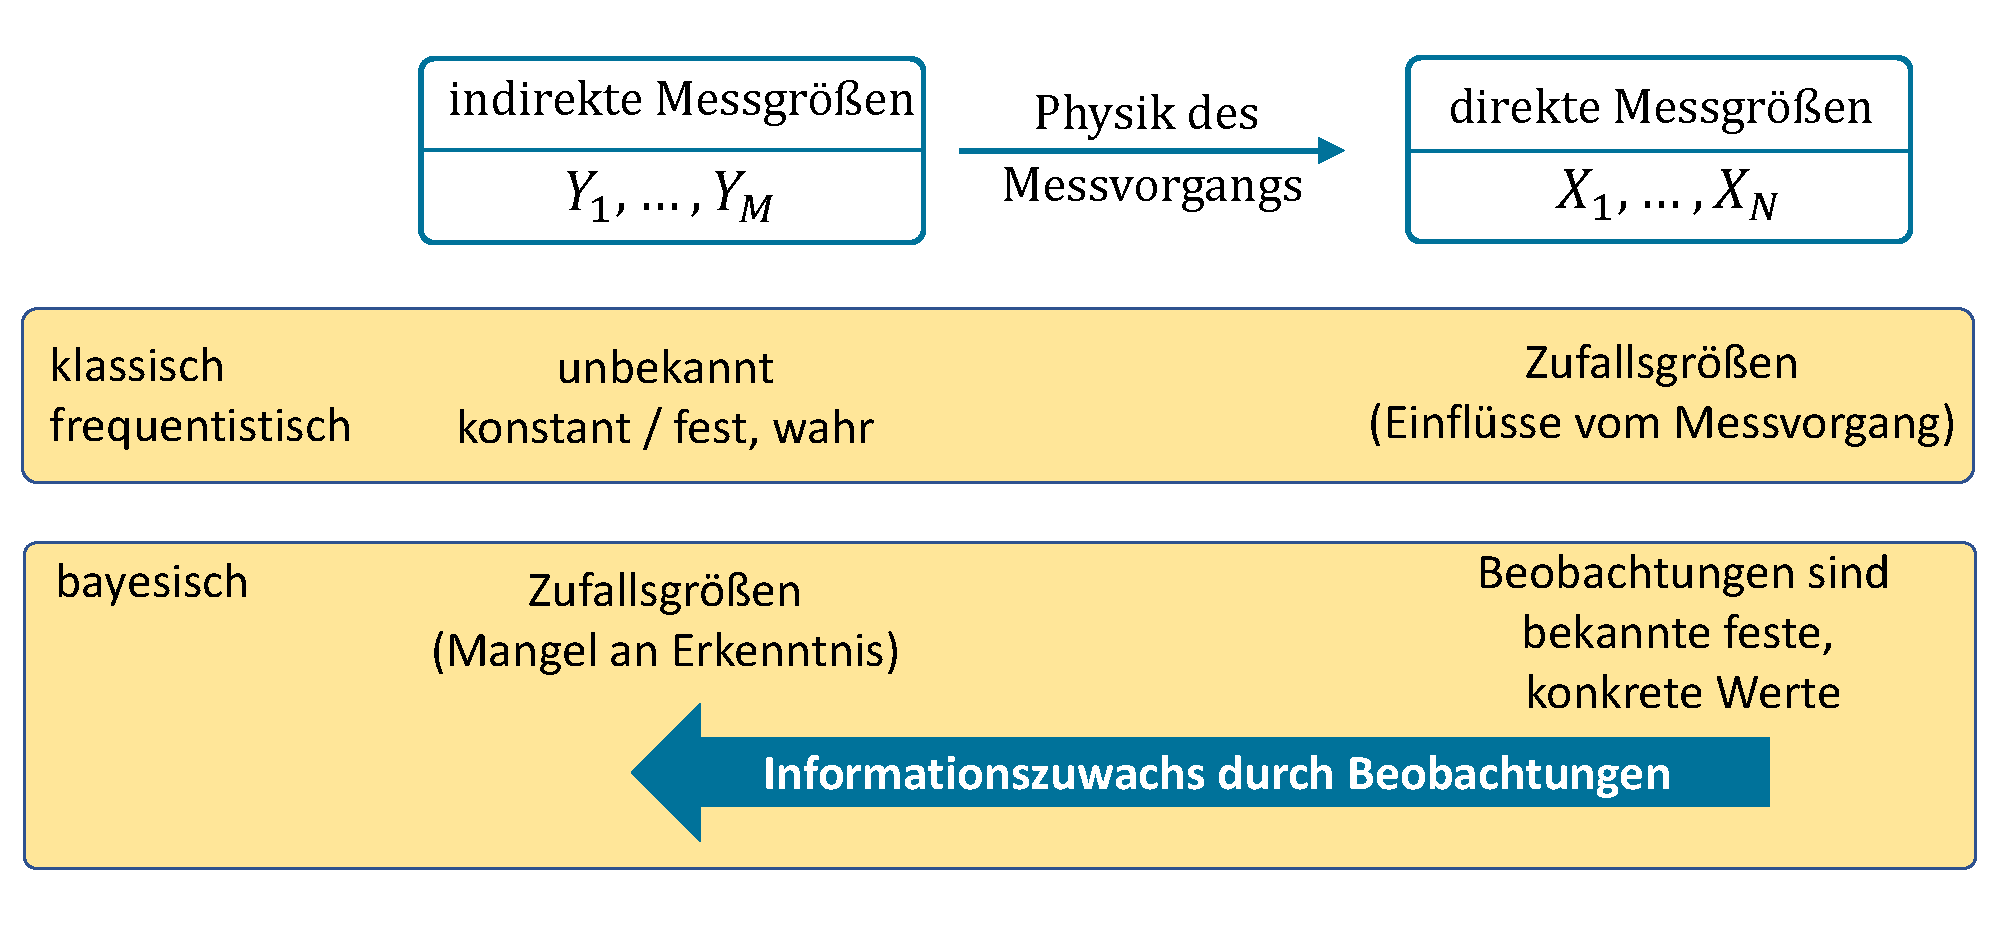
\includegraphics[width=140mm]{04_vorlesung/media/Konzept_Bayes.pdf}
\caption{Übersicht zu den Heransgehensweisen der frequentistischen und der bayesischen
Statistik}
\label{BayesFreqVergleich}
\end{center}
\end{figure}

Der Heransgehensweise, einen Informationszuwachs statistisch zu verarbeiten, liegt der \textsl{Satz von
Bayes} zu bedingten Wahrscheinlichkeiten zugrunde:
\begin{equation}
p(M | D) \; = \; \frac{p(D | M) p(T)}{p(D | M) p(M) \, + \, p(D | \lnot M) p(\lnot M)}
\label{bayestheorem}
\end{equation}
mit $M$ für die Theorie und $D$ für die Indizien (engl.\ \textsl{evidence}).


Die Theorie ist dabei
ein Modell $f$ mit Parametern $\mathbf{p}$, $\boldsymbol{\Sigma}$, die als statistisches Ereignis $M$
betrachtet wird. Die Indizien sind die Tupel von Beobachtungen zu
den direkten Messgrößen, die Daten, die ebenfalls als Ereignis $D$ betrachtet werden.
\begin{itemize}
\item $p(M)$ heißt \textsl{Prior}:

Wahrscheinlichkeit des {\`a} priori geschätzten
Modells mit $(\mathbf{p}_0, \boldsymbol{\Sigma}_0)$

\item $p(M | D)$ heißt \textsl{Posterior}:

Wahrscheinlichkeit des Modells mit Parametern $(\mathbf{p}, \boldsymbol{\Sigma})$
für die neuen Beobachtungen, also den hinzugewonnenen Datensatz
 $D = \{(X_{1,1},\dots,X_{1,J}), \dots,(X_{N,1},\dots  X_{N,J})\}$.
\end{itemize}

% ----------

Für das Verständnis, wie das Prinzip der bayesischen Statistik funktioniert,
betrachten wir das ganz einfache Beispiel Gl.~(\ref{oneQuantityOnly1}), also
 den einfachsten Fall einer einzigen Größe. Der Modellparameter $P = \mu$ repräsentiere
eine indirekte Messgröße $Y$. Die Größe $\mu$ ist aus einer Stichprobe zu schätzen.
Als {\`a} priori Information seien folgende Angaben bekannt:
\begin{itemize}
\item Der {\`a} priori Schätzwert der Modellgröße $\mu$ sei $y_0$.
\item Der {\`a} priori Schätzwert seiner Varianz $\sigma^2$ sei $s^2_0$.
\item Diese Größe sei normalverteilt, also verwenden wir als
Verteilungsdichtefunktion $p$ die Gaußverteilung.
\end{itemize}
Die neue Stichprobe $\{X_{1,1}, \dots, X_{1,J}\}$ sei vom Umfang deutlich kleiner als
die Informationsbasis, die dem {\`a} priori-Wissen zugrunde gelegen hat, so dass
für die Streuung der Varianz die $\chi^2$-Verteilung $p_{\chi^2,\nu}$
für $\nu = J-1$ Freiheitsgrade verwendet wird. Hierzu müssen wir im Stoff vorgreifen.
Diese Verteilungsdichtefunktion werden wir in der 5.\ Vorlesung behandeln.
Sie wird verwendet als Verteilungsdichte für Varianzen und ist eine schiefsymmetrische
Verteilung mit längerem Ausläufer zu größeren Werten. Je kleiner der Stichprobenumfang,
desto schiefer die Verteilung und ausgeprägter die Ausläufer.

Die gesamte Wahrscheinlichkeitsdichteverteilung $p(Y,\sigma)$ für die indirekte Messgröße
$Y$ bzw.\ deren Approximation als Modellparameter $P = \mu$ mit Streuung $\sigma$ wird als Produkt
folgender Wahrscheinlichkeiten berechnet,
\begin{itemize}
\item der Likelihood $p_\mathrm{L}$,
\item der Verteilungsdichte $p_\mathcal{N}(y | y_0, s_0)$ der Größe $\mu$ aus den {\`a} priori Informationen,
\item der Verteilungsdichte $p_{\chi^2,\nu}(s)$ der Varianz $\sigma^2$ dieser Größe.
\end{itemize}
Die zu ermittelnde bedingte Wahrscheinlichkeitsdichte wird so interpretiert, dass die Verteilung Funktion
der Variablen $\mu$ und $\sigma$ ist, gegeben die Beobachtungswerte der Stichprobe. Die Likelihood wird
dabei betrachtet als die bedingte Wahrscheinlichkeitsdichte $p_\mathrm{L}$ der
direkten Messgröße $X_1$ gegeben die Modellparameter $\mu$ und $\sigma$:
\begin{equation}
p_\mathrm{L}(\{X_{1,1}, \dots, X_{1,J}\} | \mu, \sigma) \; = \;
\prod\limits_{j=1}^J \frac{1}{\sqrt{2 \pi} \, \sigma}
 e^{- \frac{1}{2} \, \left( \frac{X_{1,j} - \mu}{\sigma} \right)^2 }  \; = \;
l(\mu, \sigma | \{X_{1,1}, \dots, X_{1,J}\}).
\end{equation}
Die Varianz $\sigma^2$ wird gemäß der $\chi^2$-Verteilung variiert. Das Variieren der Varianz
bzw.\ deren Wurzel $\sigma$ symbolisieren wir durch den Gebrauch der Variablen $s$.
Das Variieren des Modellparameters $\mu$ symbolisieren wir durch den Gebrauch der Variablen $y$.
Der Parameter $\mu$ wird ebenfalls variiert gemäß der Gaußverteilung, wir verwenden folgende
Likelihood:
\begin{equation}
p_\mathrm{L}(\{X_{1,1}, \dots, X_{1,J}\} | y, s) \; = \;
\prod\limits_{j=1}^J \frac{1}{\sqrt{2 \pi} \, s}
 e^{- \frac{1}{2} \, \left( \frac{X_{1,j} - y}{s} \right)^2 }  \; = \;
l(y, s | \{X_{1,1}, \dots, X_{1,J}\}).
\end{equation}

\begin{figure}
\begin{center}
\includegraphics[width=100mm]{04_vorlesung/media/understand_bayes_mean_posteriormatrix.pdf}
\caption{\label{posteriormatrix} Posterior-Wahrscheinlichkeitsdichte als Funktion
der beiden zu schätzenden Größen $y$ und $s$.}
\end{center}
\end{figure}
Das Produkt ist die Wahrscheinlichkeit des Modellparameters und dessen Varianz gegeben
die Stichprobe $\{X_{1,1}, \dots, X_{1,J}\}$ und die {\`a} priori Informationen $y_0, s_0$
\begin{equation}
p(y, s | \{X_{1,1}, \dots, X_{1,J}\}, y_0, s_0) \; = \; C \,
p_\mathrm{L}(\{X_{1,1}, \dots, X_{1,J}\} | y, s) \; p_\mathcal{N}(y | y_0, s_0) \; p_{\chi^2,\nu}(s)
\label{ProduktWahrscheinlichkeiten}
\end{equation}
mit $C$ als Normierungsfaktor derart zu wählen, dass die integrierte Wahrscheinlichkeit Eins ist, d.h.
$$
\int\limits_{-\infty}^\infty  \int\limits_0^\infty \; p(y, s | \{X_{1,1}, \dots, X_{1,J}\}, y_0, s_0) \;
\mathrm{d}s \, \mathrm{d}y \; = \; 1 .
$$
Die Verteilungsdichte $p(y, s | \{X_{1,1}, \dots, X_{1,J}\}, y_0, s_0)$ ist Funktion der
Variablen $y$ und $s$ mit vorgegebenen Parametern
(festen Werten) $\{X_{1,1}, \dots, X_{1,J}\}$, $y_0, s_0$, wie es beispielhaft in
Abb.~\ref{posteriormatrix} dargestellt wird.

Die Wahrscheinlichkeitsdichteverteilung
$p_\mathcal{N}(y | y_0, s_0)$ wird \textsl{Prior} genannt und die
Wahr\-schein\-lich\-keits\-dichte\-ver\-teilung $p(y, s | \{X_{1,1}, \dots, X_{1,J}\}, y_0, s_0)$
wird \textsl{Posterior} genannt.

Wir integrieren Gl.~(\ref{ProduktWahrscheinlichkeiten}) über $s$, um eine
Wahrscheinlichkeits\-dichte\-verteilung zu gewinnen, die nur noch Funktion von $y$ ist
\begin{equation}
p(y | \{X_{1,1}, \dots, X_{1,J}\}, y_0, s_0)  \; = \;
\int\limits_0^\infty p(y, s | \{X_{1,1}, \dots, X_{1,J}\}, y_0, s_0) \operatorname{d}s
\label{RandverteilungPosterior}
\end{equation}
Diese Verteilung wird \textsl{Randverteilung} oder \textsl{Marginalverteilung} genannt.
Allgemeiner gilt: Gegeben zwei Zufallsgrößen $A$ und $B$ mit gemeinsamer Verteilungsdichte
$p(A, B)$; dann heißen die Verteilungen der einzelnen Zufallsgrößen
$A$ und $B$ die Randverteilungen des Zufallsvektors $(A, B)$.

Als Schätzwert für $Y$ berechnen wir den Erwartungswert des Modellparameters $\mu$
durch Integration über alle Werte $y$ gewichtet mit der Wahrscheinlichkeitsdichte
$p(y | \{X_{1,1}, \dots, X_{1,J}\}, y_0, s_0)$ aus Gl.~(\ref{RandverteilungPosterior})
\begin{equation}
y_1 \; = \; \int\limits_{-\infty}^\infty \, y \, p(y | \{X_{1,1}, \dots, X_{1,J}\}, y_0, s_0)
\operatorname{d}y
\end{equation}
wobei wir $y_1$ mit Index $1$ schreiben, um anzuzeigen, dass dies die Revision der Schätzung des
Modellparameters $\mu \approx Y$ gegenüber vorheriger Kenntnis mit Schätzwert $y_0$ ist.

Zu einem \textsl{Messergebnis} gehört jeweils ein Intervall, das ein Maß für die Unsicherheit
des Wertes/ der Werte der Messgröße ist, siehe [VIM 2.9]

\begin{quote}
\textbf{Messergebnis}

Menge von Größenwerten, die einer Messgröße zugewiesen sind, zusammen mit jeglicher
verfügbarer relevanter Information

ANMERKUNG 1 Ein \textsl{Messergebnis} enthält im Allgemeinen \glqq relevante Information\grqq ~über
die Menge der Größenwerte, von denen einige repräsentativer für die Messgröße sein können als andere.
Dies kann in Form einer Wahrscheinlichkeitsdichtefunktion ausgedrückt werden.

ANMERKUNG 2 Ein \textsl{Messergebnis} wird im Allgemeinen
als ein einziger Messwert und eine \textsl{Messunsicherheit}
ausgedrückt. Wird die Messunsicherheit für einige
Zwecke als vernachlässigbar angesehen, kann das
Messergebnis als ein einziger Messwert ausgedrückt
werden. In vielen Bereichen ist dies die übliche Art, ein
Messergebnis auszudrücken.

ANMERKUNG 3 In der traditionellen Literatur und in der
vorhergehenden Ausgabe des VIM war das Messergebnis
als ein Wert definiert, der einer Messgröße zugewiesen
ist, und so erklärt, dass er eine Anzeige oder ein
unkorrigiertes oder ein korrigiertes Ergebnis bedeutet, je
nach Kontext.
\end{quote}

Mit der in Anmerkung~1 angesprochenen Wahrscheinlichkeitsdichtefunktion sind Verteilungen wie
die in den Gln.~(\ref{Likelihood2}) und (\ref{LikelihoodKov2}) vorgestellen Likelihoods oder
der in Gl.~(\ref{RandverteilungPosterior}) vorgestellten Posterior
mit $p(y | \{X_{1,1}, \dots, X_{1,J}\}, y_0, s_0)$ gemeint. Die Likelihood wird
für kleine Stich\-proben\-um\-fänge ($N < 100$) anstelle durch eine Gaußverteilung durch eine Verteilung
repräsentiert, deren Charakteristik im Kurvenverlauf
überhöhter und mit länger auslaufenden Rändern ist. Sie wird $t$-Verteilung genannt.
Wir werden später in der 5.\ Vorlesung auf diesen Verteilungtyp zurück kommen.

Allgemein betrachten wir für beide Fälle eine Wahrscheinlichkeitsdichtefunktion $p \! : y \mapsto p(y)$.
Der Definitionsbereich für $y$ reicht von minus bis plus Unendlich. Von Interesse ist der Kernbereich
der Dichteverteilung für eine spezifizierte Wahrscheinlichkeit $1-\alpha$, beispielsweise
$1-\alpha = 0.95$ oder $0.90$ oder so.
Dies ist die Wahrscheinlichkeit einer Größe, einen Messwert im Bereich (Intervall) $[y_\mathrm{min}, y_\mathrm{max}]$,
anzunehmen
\begin{equation}
1 \, - \, \alpha \; = \;
\int\limits_{y_\mathrm{min}}^{y_\mathrm{max}} p(y)
\operatorname{d}y .
\label{UeberdeckungWahrscheinlichkeit}
\end{equation}
Die Breite des Intervalls gibt dann die \textsl{Messunsicherheit} an.

Das Intervall $[y_\mathrm{min}, y_\mathrm{max}]$, zu dem die Fläche $1 - \alpha$ unter der die
Verteilungsdichte $p(y)$ repräsentierenden Kurve gehört, wird \textsl{Überdeckungsintervall} genannt.
Es ist der verallgemeinerte Begriff aus der Metrologie für das, was in der
\textsl{frequentistischen} Statistik \textsl{Vertrauensintervall},
engl.\  \textsl{Confidence Interval}, und in der \textsl{bayesischen} Statistik
\textsl{Glaubwürdigkeitsintervall}, engl.\ \textsl{Credible Interval},
heißt. Während der Begriff \textsl{Vertrauensintervall} in der deutschsprachigen
Literatur üblich ist, wird anstelle des Begriffs \textsl{Glaubwürdigkeitsintervall} üblicherweise
auch in der deutschsprachigen Literatur der Begriff \textsl{Credible Interval} verwendet.

Die Verwendung unterschiedlicher Bezeichnungen, \textsl{Confidence Interval} und
\textsl{Credible Interval}, soll die Unterschiedlichkeit der Vorstellungen
über den Charakter einer indirekten Messgröße $Y$ zum Ausdruck bringen.
Die Unterschiedlichkeit in der Vorstellung von einer indirekten Messgröße $Y$ besteht darin,
dass im Fall der \textsl{bayesischen} Statistik
die indirekte Messgröße $Y$ als Größe, die intrinsisch eine Zufallsgröße ist, betrachtet
wird. Im Fall der \textsl{frequentistischen} Statistik wird $Y$ als eine Größe betrachtet,
die einen festen, wahren Wert hat, der aber nicht zugänglich ist. Nur der
Modellparameter, der eine indirekte Messgröße approximiert und der indirekt aus anderen
Zufallsgrößen gewonnen wird, wird als daraus resultierend einer Streuung unterliegend betrachtet.

Die Wahrscheinlichkeit $1 - \alpha$ wird in der \textsl{frequentistischen} Statistik
\textsl{Vertrauensniveau} genannt. Die beiden Flächen unter den
Ausläufern der Dichteverteilung stellt eine Wahrscheinlichkeit $\alpha$ dar, die in der
\textsl{frequentistischen} Statistik \textsl{Signifikanzniveau} genannt wird.

Im folgenden werden wir sehen, wie eine \textsl{Messunsicherheit} im Rahmen der
\textsl{bayesischen} Statistik gewonnen wird.
Die Grenzen des \textsl{Credible Interval} $[y_\mathrm{min}, y_\mathrm{max}]$ bilden die
Integrationsgrenzen $y_\mathrm{min}$ und $y_\mathrm{max}$ der \textsl{Posterior}, so dass
\begin{equation}
1 \, - \, \alpha \; = \;
\int\limits_{y_\mathrm{min}}^{y_\mathrm{max}} p(y | \{X_{1,1}, \dots, X_{1,J}\}, y_0, s_0)
\operatorname{d}y .
\label{UeberdeckungPosterior}
\end{equation}
Die Integrationsgrenzen werden über die Umkehrfunktion der kumulativen Verteilung $P$ berechnet.
Die kumulative Verteilung $P$ ist
\begin{equation}
P(y) \; = \; \int\limits_{-\infty}^{y} p(y^\prime | \{X_{1,1}, \dots, X_{1,J}\}, y_0, s_0)
\operatorname{d}y^\prime .
\end{equation}
Die Umkehrfunktion schreiben wir symbolisch als $P^{-1}$.
Wir berechnen für das \textsl{Credible Interval}
\begin{equation}
y_\mathrm{min} \, = \, P^{-1}(\frac{\alpha}{2}) \qquad \mathrm{und} \qquad
y_\mathrm{max} \, = \, P^{-1}(\frac{1-\alpha}{2}).
\end{equation}
\begin{figure}
\begin{center}
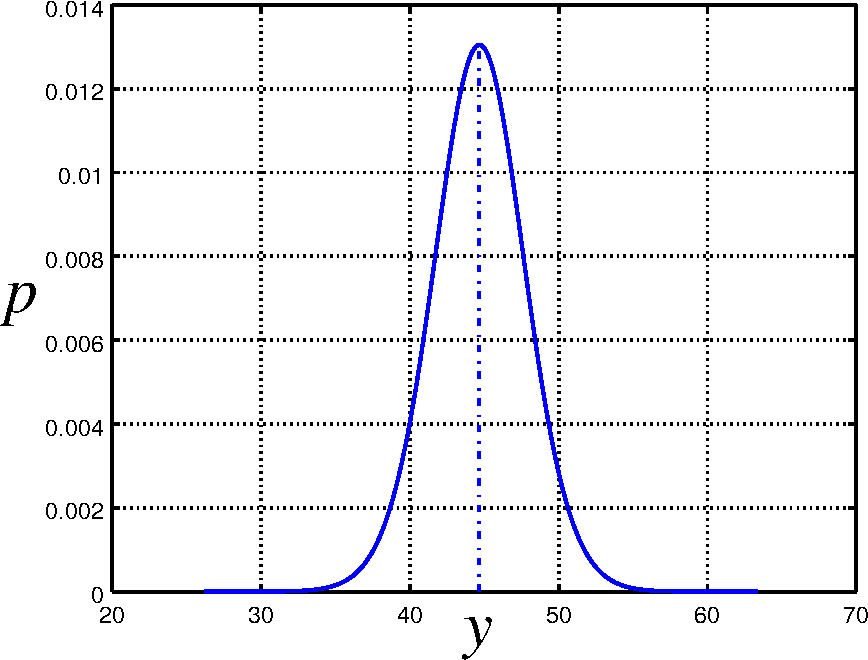
\includegraphics[width=80mm]{04_vorlesung/media/understand_bayes_mean_posteriormarginal.pdf}
\hspace{5mm}
\includegraphics[width=80mm]{04_vorlesung/media/understand_bayes_mean_cumposterior.pdf}
\caption{\label{posteriorCredible}\textsl{Links:} Die blaue Kurve stellt die
Randverteilung der Posterior-Wahrscheinlichkeitsdichte als Funktion
der beiden zu schätzenden Größen $Y$ mit \textsl{Credible Interval} dar und die
rot gestrichelte Kurve die Student-t-Verteilung mit Vertrauensintervall.
\textsl{Rechts:} Kumulierte Randverteilung der Posterior-Wahrscheinlichkeitsdichte, deren
Umkehrfunktion verwendet wird, um die Intervallgrenzen des \textsl{Credible Interval}s zu ermitteln.}
\end{center}
\end{figure}
Abb.~\ref{posteriorCredible} links zeigt im Vergleich folgende Verteilungsdichten
\begin{itemize}
\item die Posterior als Funktion des Parameters
$y$ mit einem \textsl{Credible Interval} für eine Wahrscheinlichkeit von
$1 - \alpha = 0.95$ (blaue, durchgezogene Kurve und blaue, durchgezogene Linien)
\item die $t$-Verteilung (rote, gestrichelte Kurve), die sich für die in dem
graphisch dargestellten Beispiel verwendeten Stichprobe mit Stichprobenumfang $J = 7$, folglich
$\nu = J - 1 = 6$ Freiheitsgraden ergeben hat, sowie das Vertrauensintervall (rote, gestrichelte Linien),
das aus dem Mittelwert der Stichprobe
und der empirischen Standardabweichung des Mittelwerts multipliziert mit dem
$t$-Quantil gewonnen wurde. Mit dem Begriff $t$-Quantil werden die Integrationsgrenzen dieser Verteilung
zu vorgegebenen Wahrscheinlichkeiten $\frac{\alpha}{2}$ und $1 - \frac{\alpha}{2}$ bezeichnet.
\end{itemize}

Abb.~\ref{posteriorCredible} rechts zeigt die kumulierte Posterior, aus deren Umkehrfunktion
zu den Wahrscheinlichkeiten $\frac{\alpha}{2}$ und $1 - \frac{\alpha}{2}$ die
Intervallgrenzen des \textsl{Credible Interval}s gewonnen werden.

Die Ermittlung der \textsl{Messunsicherheit} im Rahmen der
\textsl{frequentistischen} Statistik unter Verwendung der $t$-Verteilung
wird in den kommenden Wochen detailiert und mit Beispielen dargelegt werden.
Sie wird einen großen Teil dieser Vorlesungsreihe ausmachen und Klausurrelevanz haben.

%
\chapter{Wahrscheinlichkeiten und Hypothesentests}
\label{wahrscheinlichHyp}

\section{Konzept der statistischen Erwartung}

Das \textsl{Signifikanzniveau} $\alpha$ und die dazu komplementäre Wahrscheinlichkeit,
das \textsl{Vertrauensniveau} $1 - \alpha$ spielen eine zentrale Rolle bei der Bewertung
von Messergebnissen. Als wir in Kapitel~\ref{KonzepteinverseProbleme} die Konzepte der statistischen Auswertung
behandelt hatten,
haben wir diese beiden Begriffe gemeinsam mit dem des \textsl{Vertrauensintervalls} bzw.\
\textsl{Credible Interval} eingeführt, mit dem gemeinsamen Oberbegriff \textsl{Überdeckungsintervall}.
Es ist das Intervall, in dem mit einer Wahrscheinlichkeit von $P(X_1) = 1 - \alpha$ die
beobachteten Werte $X_{1,j}$ zur Größe $X_1$ liegen, das also die \glqq meisten\grqq
~Beobachtungen abdeckt.

Die Idee hinter dem Begriff des \textsl{Vertrauensintervalls} oder des \textsl{Credible Interval}s
ist, dass beim Bestimmen einer physikalischen Größe $X$ eine Vorstellung (eine Erwartung) darüber
existiert, wie die gemessenen oder beobachteten Werte verteilt sind. Das schließt die
Erwartung von Position und Breite des Bereichs, in dem die Werte liegen sollten, ein.
Diese Erwartung wird quantifiziert mit einer Angabe über die Wahrscheinlichkeit, dass die
zu messende Größe diesen oder jenen Wert annimmt, eher noch in welchem Bereich (Intervall) der
Wert zu erwarten ist. Wir \textsl{vertrauen} also darauf, dass wir einen Wert messen, der innerhalb eines
gewissen Intervalls liegen müsste, oder sagen, dass es plausibel oder \textsl{glaubwürdig}
(engl.\ \textsl{credible}) ist, dass die Beobachtungen in dem Intervall liegen.
Statt zu sagen, dass wir \textsl{eine Vorstellung haben}, können wir auch sagen,
dass wir \textsl{eine Hypothese aufstellen}.

Die Normalverteilung (Gaußverteilung) ist die grundlegende Verteilungsdichtefunktion
zur Beschreibung zufälliger Prozesse, beispielsweise Zerfallsprozesse und Diffusionsprozesse.
Bei rein stochastischen Prozessen wird von Zufallsgrößen ausgegangen, deren
Wahrscheinlichkeitsdichteverteilung eine Normalverteilung ist
\begin{equation}
p(X) \; = \; \frac{1}{\sqrt{2 \pi} \, \sigma} \, e^{-\frac{1}{2}\left(\frac{X - \mu}{\sigma}\right)^2}.
\end{equation}
Verteilungen wie die Poisson-Verteilung und die Binominal-Verteilung gehen für
unendlich viele Beobachtungen oder Stichprobenentnahmen in die Gaußverteilung über.

In der Wahrscheinlichkeitstheorie wird diese Tatsache exakt formuliert und ist der
\textsl{zentrale Grenzwertsatz} (engl.\ \textsl{central limit theorem}) CLT.
In einfacheren Worten können wir sagen:
\begin{quote}
Die Summe einer großen Anzahl von unabhängigen Zufallsgrößen folgt
asymptotisch einer stabilen Verteilung.
\end{quote}
Bei endlicher und positiver Varianz der Zufallsgrößen ist ihre Summe annähernd
normalverteilt, was die Sonderstellung der Normalverteilung erklärt.

Hierzu wird das Ziehen eines Wertes (das Machen einer Beobachtung / das Eintreten eines
Ereignisses) als Zufallsgröße interpretiert.
Damit betrachten wir eine Stichprobe als Folge von Zufallsgrößen. Sind die Elemente
einer Stichprobe Zufallsgrößen, die
\textsl{unabhängig und identisch verteilt} (Abkürzung: u.i.v.) sind, so ist auch ihre Summe
eine Zufallsgröße, die normalverteilt ist, wenn der Stichprobenumfang beliebig groß ist,
also gegen Unendlich konvergiert. In der englischsprachigen Literatur ist
\textsl{unabhängig und identisch verteilt} unter dem Begriff
\textsl{independent and identically distributed}, kurz i.i.d., zu finden.

Liegt nun eine Einzelbeobachtung innerhalb der flachen
Ausläufer (\textsl{tails}) der Wahrscheinlichkeitsdichteverteilung,
also außerhalb des Vertrauensintervalls, so
spricht man dann davon, dass der Wert (die Einzelbeobachtung)
signifikant von dem, was zu erwarten ist, abweicht. Das heißt, dass ein Ereignis eintritt,
das \textsl{nicht der Erwartung entspricht}. Somit \textsl{vermuten wir ein Problem}. Das Aufspüren
des Problems erfolgt durch \textsl{Hypothesentests}. Da die Normalverteilung
lange Ausläufer hat, gibt es eine kleine Wahrscheinlichkeit $\alpha$ dafür, dass es
weiter abseits liegende Werte gibt. Deshalb gilt es zu untersuchen,
ob solch ein Wert in der Tat im Rahmen der Normalverteilung weiter weg liegt
oder aber ob er auf Basis eines anderen Effektes gewonnen
wurde, ob er - statistisch formuliert - zu einer anderen Grundgesamtheit gehören könnte.

Der \textsl{Kolmogorow-Smirnow-Test} ist ein möglicher Test zum Prüfen, ob eine aus Beobachtungen
empirisch ermittelte Verteilung zu einer für die statistische Analyse der Beobachtungen
zugrundegelegten (erwarteten) Wahrscheinlichkeitsdichtefunktion passt.

% 30. Okt 2017

\section{Kolmogorow-Smirnow-Test}

\begin{figure}
\begin{center}
\includegraphics[width=80mm]{05_vorlesung/media/learn_robust.pdf}
\includegraphics[width=80mm]{05_vorlesung/media/learn_robust_2.pdf}
\caption{Beispiel für nicht erwartungsgemäße Beobachtungen (\textsl{rechts}) und
Umgewichten um die Verteilungform der Normalverteilung anzupassen \textsl{links}}
\label{biasExample}
\end{center}
\end{figure}
Das in Abb.~\ref{biasExample} dargestellte Beispiel zeigt dieselben Diagramme und
Daten, die wir in Abschnitt~\ref{robustEstimation} bereits zur Veranschaulichung
robuster Schätzverfahren behandelt hatten. Den robusten Schätzverfahren liegt die
im folgenden erläuterte statistische Betrachtung zugrunde: Es liegt eine Annahme
(Hypothese) darüber vor, welcher Gestalt die Wahrscheinlichkeitsverteilung der
Beobachtungen ist und ob eine Reihe von Beobachtungen zu einer gemeinsamen Verteilung
gehören oder zu unterschiedlichen Verteilungen. Technisch gesehen stellen sich die
Fragen, die statistisch formuliert lauten \glqq gehören Beobachtungen zu einer
Verteilung\grqq ~oder \glqq gehören Beobachtungen zu mehreren verschiedenen Verteilungen\grqq,
als
\begin{itemize}
\item \glqq stammen die Messwerte aus einem Prozess\grqq ~oder \glqq aus unterschiedlichen
Prozessen\grqq,
\item \glqq werden alle Messwerte von demselben Effekt beeinflusst \grqq ~oder \glqq gibt es
für verschiedene Gruppen aus der Messreihe unterschiedliche beeinflussende Effekte\grqq.
\end{itemize}
Die Annahmen bzw.\ Hypothesen bezüglich der Verteilungen zur Wahrscheinlichkeit
von Beobachtungswerten werden geprüft. Diese Art der Prüfung wird \textsl{Hypothesentest}
genannt. Es gibt unterschiedliche Typen von Hypothesentests, einer davon ist
der \textsl{Kolmogorow-Smirnow-Test}.
Er ist ein statistischer Test auf Übereinstimmung zweier Wahrscheinlichkeitsverteilungen.

Der Test verwendet die kumulierten Wahrscheinlichkeitsfunktionen
\begin{equation}
P(X) \; = \; \int\limits_{-\infty}^X \, p(X^\prime) \, \mathrm{d} X^\prime .
\end{equation}
Das hat den Vorteil, dass
die Verteilung der empirischen Häufigkeiten ohne Histogrammierung, d.h.\ ohne Einteilung in Klassen,
erfolgen kann.

Wir wollen damit prüfen, ob die Beobachtungen des in Abschnitt~\ref{robustEstimation} zur robusten
Schätzung betrachteten Beispiels der Annahme folgt, zu der Grundgesamtheit \textsl{genau einer}
Zufallsgröße $X_1$ zu gehören. Ferner nehmen wir an, dass ihre Ausprägungen (Beobachtungswerte)
unabhängig und identisch der Normalverteilung folgen.
\begin{quote}
Die Nullhypothese lautet:\\
Die Beobachtungen zu $X_1$ gehören zu einer
normalverteilten Grundgesamtheit.
\end{quote}
Wir prüfen, ob die Stichprobe $(X_{1,1}, X_{1,2}, \dots, X_{1,J})$ bezüglich
des Mittelwertes $y \, = \, \frac{1}{J} \sum_{j=1}^J X_{1,j}$ und der
empirischen Varianz $s^2 \, = \, \frac{1}{J-1} \sum_{j=1}^J (X_{1,j} \, - \, y)^2$ normalverteilt
ist. Die kumulierte Normalverteilung, mit der wir die kumulierte Verteilung der relativen Häufigkeiten
vergleichen, ist
\begin{equation}
P(X) \; = \;  \frac{1}{\sqrt{2\pi} s}
\int\limits_{-\infty}^X \, e^{-\frac{1}{2}\left(\frac{X^\prime \, - \, y}{s}\right)^2} \, \mathrm{d} X^\prime.
\label{cdfKS}
\end{equation}
Die kumulierte Gaußverteilung entspricht im wesentlichen der
Fehlerfunktion $\mathrm{erf}$, englisch \textsl{Error Function}.
\begin{equation}
\mathrm{erf}(X) \; := \; \frac{2}{\sqrt{\pi}} \; \int\limits_0^X \, e^{-X^{\prime 2}} \, \mathrm{d} X^\prime.
\label{erf}
\end{equation}
Die unterschiedlichen Definitionen für die kumulierte Gaußverteilung
und die Fehlerfuntion führen zu unterschiedlichen Wertebereichen.
Während die kumulierte Gaußverteilung einen Wertebereich von $0$ bis $1$ hat, ist die Fehlerfunktion so
definiert, dass sie einen Wertebereich von $-1$ bis $1$ hat. Sie lassen sich wie folgt in einander
überführen
\begin{equation}
P(X) \; = \; \frac{1}{2} \left(1 \, + \, \mathrm{erf}(\frac{X - y}{\sqrt{2} \, s})\right).
\end{equation}
Für standardnormalverteilte Zufallszahlen $Z = \frac{X-\mu}{\sigma}$ oder $Z = \frac{X-y}{s}$
wird für die kumulierte Gaußverteilung der Bezeichner $\Phi$ verwendet
\begin{equation}
 \Phi(Z) := \frac{1}{\sqrt{2\pi}}
\int\limits_{-\infty}^Z \, e^{-\frac{1}{2} Z^{\prime 2} } \, \mathrm{d} Z^\prime
\quad \Rightarrow \quad
\Phi(Z) \; = \; \frac{1}{2} \left(1 \, + \, \mathrm{erf}(\frac{Z}{\sqrt{2}})\right).
\label{cdfPhi}
\end{equation}

Die Kenntnis dieser unterschiedlichen Definitionen und wie sie ineinander umzurechnen sind ist
wichtig, weil die statistischen Bibliotheksfunktionen von Matlab, Gnu-Octave, Python, etc.\
nicht die kumulierte Gaußverteilung bzw.\ die kumulierte Standardnormalverteilung, sondern die Fehlerfunktion
zur Verfügungs stellen.

Die kumulierte Verteilung der relativen Häufigkeiten gewinnen wir darüber, dass wir die Werte der
Stichprobe in aufsteigender Reihenfolge sortieren
\begin{equation}
X_{1,k_1} \, \leq \, X_{1,k_2} \, \leq \,  \dots \, \leq \,  X_{1,k_J}
\end{equation}
Die Teilstichprobe mit der Beobachtung mit dem kleinsten Wert $(X_{1,k_1})$ hat die
relative kumulierte Häufigkeit $\frac{1}{J}$, die Teilstichprobe mit den zwei
kleinsten Beobachtungen $(X_{1,k_1}, X_{1,k_2})$ hat die relative kumulierte Häufigkeit $\frac{2}{J}$.
Die Teilstichprobe mit den $j$ kleinsten Beobachtungen
\begin{equation}
(X_{1,k_1}, X_{1,k_2}, \dots, X_{1,k_j})
\quad \text{hat~die~relative~kumulierte~Häufigkeit}
\quad H(X_{1,k_j}) \; = \; \frac{j}{J}
\label{cdfH}
\end{equation}
\begin{figure}
\begin{center}
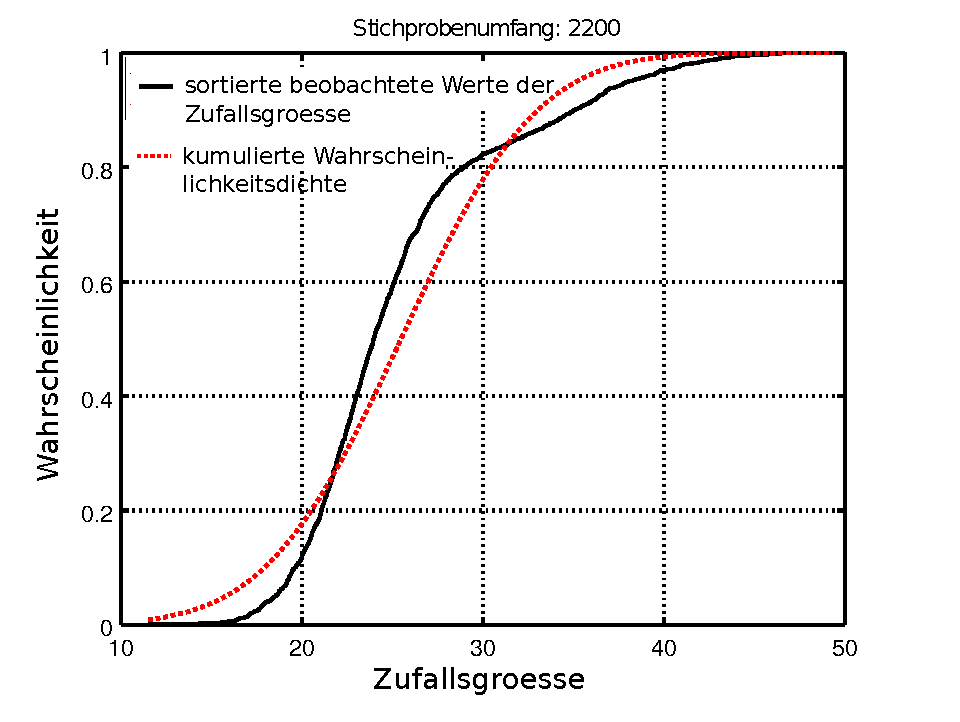
\includegraphics[width=100mm]{05_vorlesung/media/KS_pdf_iteration0.pdf}
\caption{\label{cdf4KStest} Vergleich der Wahrscheinlichkeiten (kumulierte Verteilungsdichten) aus der
empirische gewonnenen Häufigkeit der beobachteten Werte der Zufallsgröße
(schwarze, durchgezogene Kurve) mit der kumulierten Normalverteilung, die sich auf
die empirischen Erwartungswerte, den Mittelwert und die empirische Varianz, bezieht (rote,
gestrichelte Kurve).}
\end{center}
\end{figure}

Abb.~\ref{cdf4KStest} stellt zum Vergleich die Wahrscheinlichkeitsfunktion
(kumulierte Verteilungsdichte) $P(X)$ gemäß Gl.~(\ref{cdfKS})
als rote, gestrichelte Kurve und die kumulierte, relative Häufigkeit
$H(X_{1,k_j}) \; = \; \frac{j}{J}$
als schwarze, durchgezogen gezeichnete Kurve in einem Diagramm dar.


Die Prüfgröße des \textsl{Kolmogorow-Smirnow}-Tests ist
\begin{equation}
\arraycolsep=2.4pt\def\arraystretch{2}
\begin{array}{l}
\sup\limits_{X} \mid H(X_{1,k_j}) \, - \, P(X) \mid \; = \;\\
\max\limits_{k_j} \left\{ \max \left\{ \mid H(X_{1,k_j}) \, - \, P(X_{1,k_j}) \mid, \;
\lim\limits_{X \rightarrow X_{1,k_j}} \mid H(X) \, - \, P(X_{1,k_j} - 1) \mid \right\} \; \right\} .
\end{array}
\end{equation}
Dabei steht sup für Supremum, was \textsl{kleinste obere Schranke} heißt.
Zu jeder Ausprägung der Stich\-probe wird der Betrag der Differenz der beiden
Wahrscheinlichkeiten berechnet. Die Berechnung des Grenzwertes
$\lim\limits_{X \rightarrow X_{1,k_j}} \mid H(X) \, - \, P(X_{1,k_j} - 1) \mid$
für das Supremum ist erforderlich, wenn die kumulierte relative Häufigkeit
(Summenhäufigkeit) durch Kumulieren eines Histogramms, also einer in Klassen
quantisierten Stichprobe, berechnet wurde. Dabei soll die Schreibweise mit
dem Grenzwert
$$
\lim\limits_{X \rightarrow X_{1,k_j}} \mid H(X) \, - \, P(X_{1,k_j} - 1) \mid
$$
zum Ausdruck bringen, dass man infinitesimal dicht aber doch prinzipiell rechts
von $X_{1,k_j}$ an der Stufe ist, praktisch wird aber direkt
$\mid H(X_{1,k_j}) \, - \, P(X_{1,k_j} - 1) \mid$
berechnet. Für die nichtklassierte, sortierte Stichprobe berechnen wir einfach nur
\begin{equation}
\max\limits_{k_j} \left\{ \mid H(X_{1,k_j}) \, - \, P(X_{1,k_j}) \mid \right\} .
\end{equation}

Die Wahrscheinlichkeit, dass die Beobachtungen nicht zur in der Hypothese angenommenen
Verteilung passt, ist die Wahrscheinlichkeit, dass die Beobachtung
in den Ausläufern (\textsl{Tails}) der Dichteverteilung liegt, weshalb wir
die durch die Fläche in den \textsl{Tails} repräsentierte Wahrscheinlichkeit mit
\textsl{Signifikanzniveau} $\alpha$ bezeichnen.

Beim Kolmogorow-Smirnow-Test wird die Nullhypothese verworfen, wenn
die empirische relative Häufigkeit einen Grenzwert überschreitet,
der vom Signifikanzniveau $\alpha$ und dem Stichprobenumfang $J$ abhängt
\begin{equation}
\sup\limits_{X} \mid H(X_{1,k_j}) \, - \, P(X) \mid \; > \; K_{\alpha, J}
\end{equation}
wobei es zu Schwellwerten $K_{\alpha, J}$ für $J < 35$ Tabellen in den gängigen
Formelsammlungen gibt und
für $J \geq 35$ folgende Näherung verwendet wird:
\begin{equation}
K_{\alpha, J} \; = \; \sqrt{-\frac{1}{2 \, J} \, \ln(\frac{\alpha}{2})}
\label{KSpruefgroesse}
\end{equation}


Hypothesentests in Python (\href{https://mybinder.org/v2/gh/dhueser/MDA-Vorlesung-iprom-tu-bs/master?urlpath=/lab/tree/vorlesung/05_vorlesung/code/hypothesentests.ipynb}{Klicke hier für interaktive Session}):
\lstinputlisting[style=Python]{05_vorlesung/code/example_KSTest.py}


\section{Wahrscheinlichkeitsdichtefunktionen und ihre Parameter}

Bei vielen beobachteten Stichproben, die signifikant von dem Modell, das besagt, dass sie zu genau einer
normalverteilten Grundgesamtheit gehören, abweichen, handelt
es sich um Beobachtungen aus Prozessen, denen mehrere überlagerte stochastische Anteile
zugrunde liegen. Bei dem in Abb.~\ref{biasExample} illustrierten Beispiel waren dies
zwei normalverteilte Grundgesamtheiten mit verschiedenen Erwartungswerten $\mu_1$ und
$\mu_2$ und mit unterschiedlichen Varianzen $\sigma^2_1$ und $\sigma^2_2$.

Für eine Bewertung von gemessenen Werten einer Größe, d.h.\ von Beobachtungen, werden statistische
Modelle zugrunde gelegt. Ein statistisches Modell zu beobachtbaren Größen umfasst die
Vorstellung von Zufallsgrößen und der Verteilung ihrer Beobachtungswerte.
Wahrscheinlichkeitsdichtefunktionen werden parametrisiert über ihre statistischen Momente.
Diese charakterisieren den Kurvenverlauf der Funktion hinsichtlich ihrer Lage, Breite,
Symmetrie und so weiter.

Der \textsl{Erwartungswert einer Zufallsgröße} $X$ ist das erste statistische Moment
der Verteilungsdichte $p$ ihrer Grundgesamtheit
\begin{equation}
\mathrm{E}(X) \; = \; \int\limits_{-\infty}^{\infty} \, X \, p(X) \, \mathrm{d} X \; =: \; \mu^{(1)}(X)
\end{equation}
das ihren Schwerpunkt angibt.
Der Erwartungswert der \textsl{Varianz}
einer Zufallsgröße $X$ entspricht dem zweiten statistischen Moment
der Verteilungsdichte $p$.
Das zweite statistische Moment ist definiert durch
\begin{equation}
\int\limits_{-\infty}^{\infty} \, X^2 \, p(X) \, \operatorname{d} X \; =: \; \mu^{(2)}(X)
\end{equation}
und die Varianz ist das zweite Moment der um den Erwartungswert verschobenen Zufallsgröße
\begin{equation}
\operatorname{Var}(X) \; = \; \int\limits_{-\infty}^{\infty} \, (X - \operatorname{E}(X))^2 \,
 p(X) \, \mathrm{d} X
\end{equation}
deren Wurzel
\begin{equation}
\sigma \; = \; \sqrt{\operatorname{Var}(X)}
\end{equation}
ein Maß für die Breite von $p$ darstellt.
Die Schiefe einer Verteilungsdichte wird durch das dritte statistische Moment
\begin{equation}
\int\limits_{-\infty}^{\infty} \, X^3 \, p(X) \, \mathrm{d} X \; =: \; \mu^{(3)}(X)
\end{equation}
gewonnen, bei dem die Zufallsgröße um ihren Erwartungswert verschoben und auf die Wurzel ihrer
Varianz normiert
\begin{equation}
\operatorname{Skew}(X) \; = \; \int\limits_{-\infty}^{\infty} \, \left(\frac{X - \mathrm{E}(X)}{\sigma}
\right)^3 \, p(X) \, \operatorname{d} X
\end{equation}
wird. Das dritte statistische Moment der normierten Zufallsgröße heißt
\textsl{Skewness}.

Ein Maß für die Überhöhung oder Abflachung relativ zur Normalverteilung wird durch
das vierte statistische Moment
\begin{equation}
\int\limits_{-\infty}^{\infty} \, X^4 \, p(X) \, \mathrm{d} X \; =: \; \mu^{(4)}(X)
\end{equation}
gewonnen, bei dem die Zufallsgröße um ihren Erwartungswert verschoben und auf die Wurzel ihrer
Varianz normiert
\begin{equation}
\operatorname{Kurt}(X) \; = \;  \int\limits_{-\infty}^{\infty} \, \left(\frac{X - \operatorname{E}(X)}{\sigma}
\right)^4 \, p(X) \, \operatorname{d} X
\end{equation}
wird. Das vierte statistische Moment der normierten Zufallsgröße heißt
\textsl{Kurtosis}.

% ======

%Die Kombination der Wahrscheinlichkeitsverteilungen von mehreren unabhängigen kontinuierlichen
%Zufallsgrößen $X_1, \dots, X_N$ haben wir in den vergangenen Vorlesungen bereits kennengelernt,
%als wir die Berechnung der Likelihood und der Posterior besprochen haben.
%Bei der Likelihood wurde jede Beobachtung als von jeder anderen Beobachtung unabhängige
%Zufallszahl mit gleichen Varianzen (identische Verteilungen) behandelt.
%Beim Posterior wurden die Größen, zu
%denen als {`a} priori Informationen ein Erwartungswert und eine Varianz gegeben sind,
%als jeweilige Zufallsgrößen behandelt. Mit Zufallsgrößen $X_1, \dots, X_N$ können
%auch verschiedene Messgrößen sein, wie beispielsweise Strom und Widerstand (hier $N=2$),
%oder drei Koordingaten im Raum ($N=3$), oder zwei Positionskoordinaten auf einem CCD-Chip
%gemeinsam mit dem jeweiligen Intensitätswert ($N=3$).

%Gegeben seien $N$ Zufallsgrößen $X_1, \dots, X_N$ und zu jeder Zufallsgröße
%sei eine Wahrscheinlichkeitsdichteverteilung $p(X_i)$ mit $i=1,\dots,N$ gegeben.
%Dabei sei $p$ eine beliebige Verteilung. Sie muss keine Normalverteilung sein.
%Die Zufallsgrößen seinen kontinuierlich, es gelte $X_i \in I \!\! R$ und für den Zufallsvektor
%$\mathrm{X} = (X_1, \dots, X_N) \in I \!\! R^n$.
%Dann gilt unter der Voraussetzung, dass sie unabhängig voneinander sind, für die gemeinsame Wahrscheinlichkeitsdichteverteilung $p(X_1, \dots, X_N)^\mathsf{T} = p(\mathbf{X})$:
%\begin{equation}
%p(\mathrm{X}) \; = \;
%\frac{1}{\int\limits_{-\infty}^{+\infty} \dots \int\limits_{-\infty}^{+\infty}
%\prod\limits_{i=1}^N p(X_i^\prime) \mathrm{d} X_1^\prime \dots \mathrm{d} X_N^\prime}
%\prod\limits_{i=1}^N p(X_i) .
%\end{equation}
%Wir wollen uns die Verteilung für zwei Zufallsgrößen, also $\mathbf{X}^\mathsf{T} = (X_1,X_2)$,
%für den Fall, dass beide Zufallgrößen normalverteilt seien genauer anschauen
%\begin{equation}
%p(\mathbf{X}) = \frac{1}{2 \pi \sigma_1 \sigma_2} \,
%e^{-\frac{1}{2} \,
%  \left(\frac{X_1-\mu_1}{\sigma_1}\right)^2
%  \, - \, \frac{1}{2} \,  \left(\frac{X_2-\mu_2}{\sigma_2}\right)^2}
%\end{equation}

% 6. Nov. 2017

\section{Vertrauensintervall und t-Verteilung}

Wir hatten bereits in Kapitel \ref{KonzepteinverseProbleme} angesprochen, wie
\textsl{Vertrauensintervall} $[x_1, x_2]$, Wahrscheinlichkeistdichtefunktion $p$,
\textsl{Signifikanzniveau} $\alpha$ und \textsl{Vertrauensniveau} $1-\alpha$ zusammen hängen.
Das Vertrauensintervall gibt den Bereich an, in dem ein Ereignis mit
Wahrscheinlichkeit $1-\alpha$ beobachtet wird bzw.\ die Messgröße einen Wert in diesem Bereich
annimmt, also
\begin{equation}
\int\limits_{x_1}^{x_2} p(X) \, \operatorname{d} X \; = \; 1 - \alpha .
\end{equation}
Eine Wahrscheinlichkeitsdichteverteilung $p(X)$
wird immer so normiert, dass ihre Fläche $1$ ist:
\begin{equation}
\int\limits_{-\infty}^\infty p(X) \, \operatorname{d} X \; = \; 1
\end{equation}
Das heißt mit anderen Worten:
Unsere Größe nimmt mit Wahrscheinlichkeit $1$ irgend einen beliebigen
Wert zwischen minus und plus Unendlich an.

Auch hatten wir in Kapitel \ref{KonzepteinverseProbleme} durchgenommen, wie man aus unterschiedlichen vorliegenden
Informationen eine Wahrscheinlichkeitsdichteverteilung berechnet, um den
Erwartungswert
\begin{equation}
E(X) \; = \; \int\limits_{-\infty}^\infty \, X  p(X) \, \operatorname{d} X
\end{equation}
zu bestimmen und um aus der Umkehrfunktion $P^{-1}$ der kumulativen Verteilung
das Über\-deck\-ungs\-intervall
\begin{equation}
[P^{-1}(\frac{\alpha}{2}), P^{-1}(1-\frac{\alpha}{2})]
\end{equation}
zu ermitteln.

Man kann zur Berechnung eines Überdeckungsintervalls
rechenzeiteffizient auf vorhandene tabellierte Werte für
die Umkehrfunktion der Normalverteilung zurück greifen, wenn
folgendes der Fall ist:
\begin{itemize}
\item Über die reinen Beobachtungen $X_{1,j}$ hinaus liegen keine
Informationen vor, also keine vorherigen Ergebnisse zu den zu
schätzenden Modellparameter (kein \textsl{Prior})
und keine weiteren beeinflussenden Verteilungen.
\item Es kann davon ausgegangen werden, dass die
einzelnen Beobachtungswerte um das Modell
normalverteilt streuen.
\end{itemize}
Für kleine
Stichprobenumfänge wird eine der Normalverteilung ähnliche Verteilung
herangezogen, die je kleiner der Stichprobenumfang ist, um so stärker ausgeprägte
Ausläufer (\textsl{Tails}) hat, die $t$-Verteilung. Diese werden wir im Laufe
dieses Kapitels beleuchten.

Zunächst erörtern wir die Berechnung der Vertrauensintervalle auf Basis
tabellierter Werte von Integrationsgrenzen zu ausgesuchten Ver\-trauens\-niveaus
der Normalverteilung. Eine solche Integrationsgrenze wird \textsl{Quantil}
genannt. Die Tabellen beziehen sich auf normierte Zufallsgrößen.
Für die Gaußverteilung normieren wir die Zufallsgröße, so dass der
Erwartungswert $\mu = 0$ ist und die Varianz $\sigma^2 = 1$, d.h.
$Z$ ist \textsl{standardnormalverteilt}
\begin{equation}
Z \; \sim \; \mathcal{N}(0,1) .
\label{standardNormalverteilt}
\end{equation}
Die Wahrscheinlichkeitsdichtefunktion $p(Z)$ ist die \textsl{Standard}normalverteilung
\begin{equation}
p(Z) \; = \; \frac{1}{\sqrt{2 \pi}} \, e^{-\frac{1}{2} Z^2}
\qquad \textrm{mit} \qquad Z \; = \; \frac{X - \mu}{\sigma} .
\end{equation}

Die in den Formelsammlungen und Tabellenwerken aufgelisteten Grenzen sind
als obere Integrationsgrenze definiert
\begin{equation}
\int\limits_{-\infty}^{z_\alpha} p(Z) \mathrm{d} Z \; = \; \alpha .
\label{WahrscheinlichkeitQuantil}
\end{equation}
In Abb.~\ref{normVertQuantil} wird dies anhand des Quantils $z_\alpha = 0.5244$
zu $\alpha = 0.7$ also $70 \%$ Wahrscheinlichkeit beispielhaft gezeigt.

\begin{figure}
\begin{center}
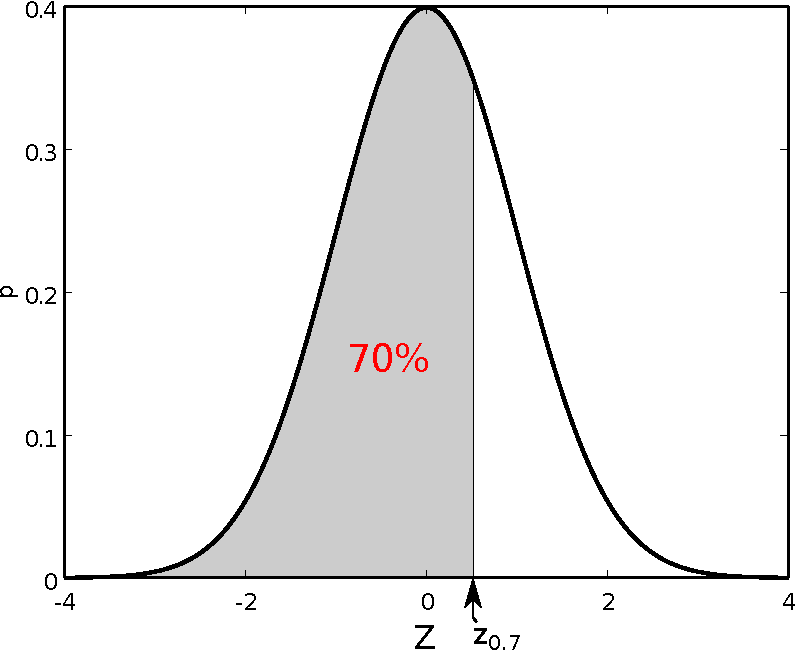
\includegraphics[width=79mm]{05_vorlesung/media/normpdfQuantil.pdf}
\hspace{5mm}
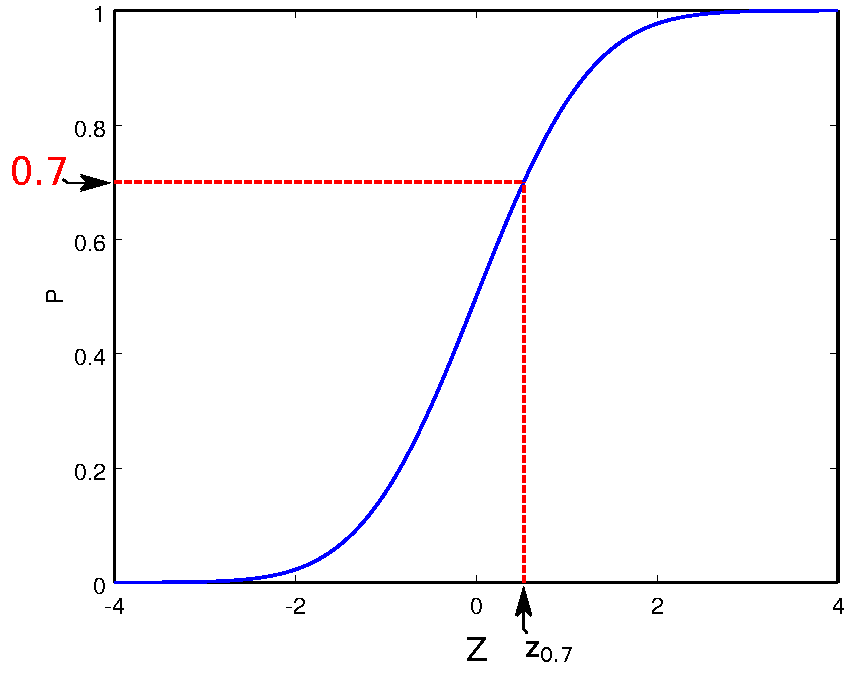
\includegraphics[width=81mm]{05_vorlesung/media/normcdfQuantil.pdf}
\caption{\label{normVertQuantil} Quantil $z_\alpha = 0.5244$ und Wahrscheinlichkeit
$\alpha = 0.7$ der Standard\-normalverteilung.}
\end{center}
\end{figure}

Dies lesen wir so:
\begin{quote}
Die Ereignisse Werte zu $Z$ zu beobachten, die kleiner sind als $z_\alpha$, können
mit einer Wahrscheinlichkeit von $\alpha$ eintreten.
\end{quote}
Die in den Tabellenwerken gelisteten Wahrscheinlichkeiten $\alpha$ werden
aus der Integration der Wahrscheinlichkeitsdichte der normierten Zufallsgröße
von minus Unendlich bis zu einer endlichen oberen Integrationsgrenze $z_\alpha$
gewonnen.
Die zu einem Wert eines Quantils gehörende Wahrscheinlichkeit wird durch den tiefgestellten
Index bei $z_\alpha$ gekennzeichnet, in unserem Beispiel aus Abb.~\ref{normVertQuantil}
ist dies dann
$$
z_{0.7} \; = \; 0.5244
$$
Als weiteres Beispiel betrachten wir die Frage, wie hoch die Wahrscheinlichkeit ist,
Werte zu beobachten, die in den Ausläufern einer Verteilungsdichte liegen.
Die Ausläufer werden im Englischen
als \textsl{Tails} (Schwänze) bezeichnet. Dies sollen Beobachtungen zu der normierten
Zufallsgröße $Z$ mit Werten, die zum einen kleiner oder gleich $-1.960$ sind, sein
$$
z_{0.025} \; = \; -1.960
$$
und zum anderen, die Beobachtungen mit Werten größer oder gleich $1.960$, also die
in dem rechten Ausläufer (\textsl{Tail}) der Standardnormalverteilung liegen.
Die Wahrscheinlichkeit für Beobachtungen im linken \textsl{Tail} ist
\begin{equation*}
\int\limits_{-\infty}^{-1.960} p(Z) \mathrm{d} Z \; = \; 0.025 .
\end{equation*}

Aufgrund der Symmetrie der Standardnormalverteilung ist die Wahrscheinlichkeit für das Liegen von
Werten im rechten \textsl{Tail} ebenfalls $0.025$. Wir rechnen also zusammen, dass mit
einer Wahrscheinlichkeit von $0.05 = 0.025+0.025$ Werte in den beiden \textsl{Tails} außerhalb
des Intervalls $[-1.960, 1.960]$ liegen können. Somit ist die Wahrscheinlichkeit, dass sie
innerhalb des Intervalls liegen $1 - 0.05 = 0.95$
\begin{equation}
\int\limits_{-1.96}^{1.96} \, p(Z) \, \operatorname{d} Z \; = \; 0.95
\end{equation}
was uns zeigt, wie wir die Tabellen zu verwenden haben.
Wenn wir ein zweiseitiges Intervall betrachten wollen, wie hier zu einem Vertrauensniveau
von $95 \%$, so müssen wir im Tabellenwerk nach dem Quantil, das für $97.5 \%$ gelistet
ist, schauen
$$
z_{0.975} \; = \; 1.960
$$
weil
$$
0.95 \; = \;
\underbrace{\int\limits_{-\infty}^{z_{0.975}} \, p(Z) \, \operatorname{d} Z}_{0.975} \; - \;
\underbrace{\int\limits_{-\infty}^{z_{0.025}} \, p(Z) \, \operatorname{d} Z}_{0.025}
$$
Aufgrund der Achssymmetrie der Normalverteilung gilt
$$
z_{\frac{1}{2}\alpha} = -z_{1-\frac{1}{2}\alpha} .
$$
Da sich die Quantile zum jeweiligen Vertrauensniveau $1-\alpha$ auf die normierte Zufallsgröße
beziehen, muss für die Berechnung des Vertrauensintervalls zurückgerechnet werden
\begin{equation}
Z \; = \; \frac{X - \mu}{\sigma} \qquad \Leftrightarrow \qquad X \; = \; \mu + Z \sigma
\end{equation}
also
\begin{equation}
[z_{\frac{1}{2}\alpha}, z_{1-\frac{1}{2}\alpha}] =
[-z_{1-\frac{1}{2}\alpha}, z_{1-\frac{1}{2}\alpha}]
 \qquad \Leftrightarrow  \qquad
[\mu \, - \, z_{1-\frac{1}{2}\alpha} \, \sigma, \mu \, + \, z_{1-\frac{1}{2}\alpha} \, \sigma]
\end{equation}
Mit $\alpha$ sind die $5 \%$ Signifikanzniveau und mit $1-\alpha$ die $95 \%$ Vertrauensniveau gemeint.

Die Likelihood wird maximal für
\begin{equation}
y \; = \; \frac{1}{J} \sum_{j=1}^J X_{1,j} ,
\end{equation}
wobei $y$ der Schätzwert für den Modellparameter $Y$ ist.
Der Schätzwert $s^2$ für die Varianz $\sigma^2$ wird berechnet mit
\begin{equation}
s^2 \; = \; \frac{1}{J-1} \sum_{j=1}^J (X_{1,j} - y)^2 .
\end{equation}

Nachdem wir gesehen haben, wie wir für eine normalverteilte Zufallsgröße
das Vertrauensintervall ermitteln können, wenden wir uns jetzt der Thematik zu,
was passiert, wenn wir zu einer Zufallsgröße nur relativ wenige Beobachtungen haben.

%------------------- kleine Stichprobenumfaenge -> Motivation t-Verteilung
\begin{figure}
\begin{center}
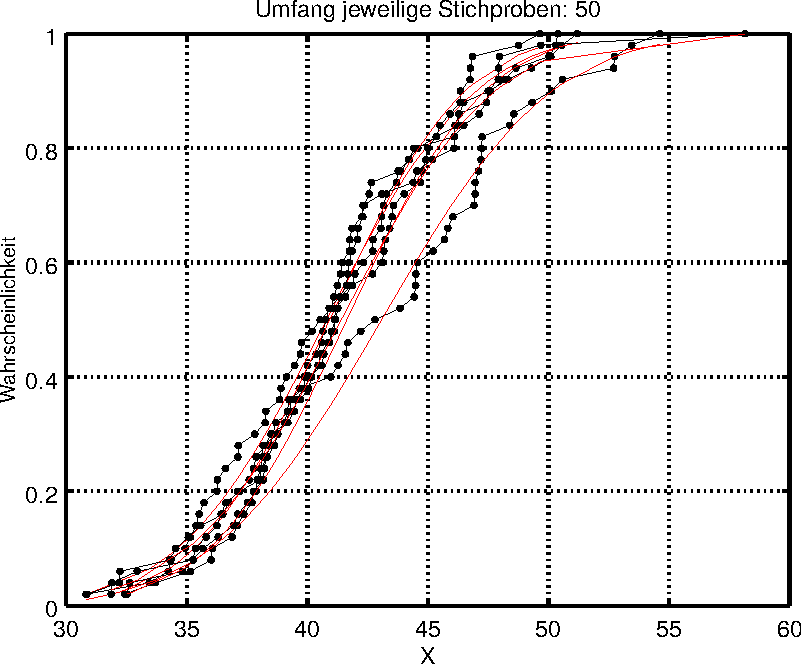
\includegraphics[width=100mm]{05_vorlesung/media/learn_Student_t1samples.pdf}
\caption{\label{kumulWahrsch} Kumulative relative Wahrscheinlichkeitsfunktionen und relative
Summenhäufigkeiten von verschiedenen Stichproben mit jeweils $J \, = \ 50$ Werten, entnommen aus einer
Grundgesamtheit mit $\mu \, = \, 42$ und $\sigma \, = \, 5$.}
\end{center}
\end{figure}
Wenn wir aus einer sehr großen Stichprobe, die einer Grundgesamtheit entnommen wurde,
disjunkte Teilstichproben von kleinerem Umfang ($J < 100$) in Grüppchen unterteilen, so können wir
beobachten, dass sowohl die Mittelwerte streuen als auch die Varianzen.
Diese Grüppchen oder Teilstichproben können wir als mehrere Stichproben aus einer normalverteilten
Grundgesamtheit ansehen.
Abb.~\ref{kumulWahrsch} illustriert wie unterschiedlich die Verteilungsfunktionen von
Stichproben mit relativ kleinem Umfang ($J \, = \ 50$) aussehen können, obwohl sie zu derselben
Grundgesamtheit gehören. Dieses Beispiel wurde wie folgt mit Gnu-octave generiert:

\lstinputlisting[style=Matlab]{05_vorlesung/code/example_t.m}

Zur Bewertung der Flachheit bzw.\ Ausgeprägtheit der Ausläufer einer Verteilung berechnen wir
ihre \textsl{Kurtosis}. Die \textsl{Kurtosis} der Normalverteilung hat den Wert $3$.

Die empirischen Schätzer für den Erwartungswert, die Varianz, die Skewness und Kurtosis
berechnen wir aus einer Stichprobe mit Beobachtungswerten $X_{1,1}, \dots, X_{1,J}$
wie folgt:
\begin{itemize}
\item[] Der Mittelwert wird berechnet mit
\begin{equation}
y \; = \; \frac{1}{J}\sum_{j=1}^J \, X_{1,j} .
\end{equation}
\item[] Die empirische Standardabweichung wird berechnet mit
\begin{equation}
s \; = \; \sqrt{ \frac{1}{J-1}\sum_{j=1}^J \, (X_{1,j} - y)^2 }.
\label{empirischeStd}
\end{equation}
Zu bemerken ist, dass jetzt durch $J-1$ und nicht durch $J$ geteilt wird, weil
das $y$ aus den Werten der Stichprobe $X_{1,1}, \dots, X_{1,J}$ gewonnen wurde und somit
die Anzahl der Freiheitsgrade $\nu$ um Eins verringert wird, also $\nu = J-1$.
\item[]
Die empirische Skewness wird berechnet mit
\begin{equation}
\textrm{skew} \; = \; \frac{1}{J} \sum_{j=1}^J \, \left( \frac{X_{1,j} - y}{s} \right)^3 .
\end{equation}
\item[] Die empirische Kurtosis wird berechnet mit
\begin{equation}
\textrm{kurt} \; = \; \frac{1}{J} \sum_{j=1}^J \, \left( \frac{X_{1,j} - y}{s} \right)^4 .
\end{equation}
\end{itemize}
Bei dem in Abb.~\ref{kumulWahrsch} gezeigten Beispiel mit mehreren Stichprobenentnahmen aus
einer Grundgesamtheit erhalten wir folgende aus den Momenten abgeleiteten empirischen
Parameter der Verteilungen:
\begin{center}
Tabelle 1:

\begin{tabular}{c||c|c|c|c}
\hline
\multicolumn{5}{c}{Einzelstichproben, Umfang jeweils $J = 50$}\\
\hline
lfd.\ Nr. & $y$ & $s$ & skew & kurt\\
\hline\hline
1 & 40.79 &  4.83 &  0.33 &  2.50 \\
2 & 43.08 &  5.52 &  0.16 &  2.16 \\
3 & 40.92 &  4.38 & -0.26 &  2.57 \\
4 & 41.64 &  4.46 &  0.09 &  2.44 \\
5 & 41.41 &  4.98 &  0.59 &  4.16 \\
\hline\hline
\multicolumn{5}{c}{alle Stichproben zusammen, Umfang $J = 5 \cdot 50 = 250$}\\
\hline
 & 41.57 &  4.88 &  0.28 &  2.89 \\
\hline\hline
\multicolumn{5}{c}{wahre Grundgesamtheit}\\
\hline
 & $\mu$ & $\sigma$ & Skew & Kurt\\
\hline\hline
Normalvert. & 42.00 &  5.00 &  0.00 &  3.00 \\
\hline
\end{tabular}
\end{center}
%--------------------- Ende der Motivation fuer t-Verteilung

%==========
%Bei einer Überlagerung unterschiedlicher Prozesse, wie dies beispielsweise
%bei exponetiell verlaufenden Zerfällen (aus der Biologie oder Strahlenphysik) der Fall ist, sind die
%Verteilungen asymmetrisch und können z.B.\ mit einer Poissonverteilung beschrieben werden.

Man kann der Beschreibung einer kleinen Stichprobe besser gerecht werden, wenn die
Verteilung flacher ist als eine Standardnormalverteilung. Das bedeutet, dass ihre Ausläufer
ausgeprägter sind.
Eine Verteilungsdichtefunktion, die der Gaußverteilung ähnlich ist, aber unter
Berücksichtigung des begrenzten Stichprobenumfangs entsprechend ausgeprägtere Tails hat,
ist die im folgenden dargestellte \textsl{Student-t}-Verteilung, kurz auch
einfach $t$-Verteilung genannt.

%==================

%-----------------
Diese Wahrscheinlichkeitsdichteverteilung wurde anfang des 20. Jahrhunderts von
William Sealy Gosset entwickelt. Sie wird der
Tatsache gerecht, dass die Varianz zunimmt mit kleiner werdendem Stichprobenumfang.
Gosset veröffentlichte 1908 erstmals zu dem Thema während er als Chemiker für die Guinness-Brauerei
in Dublin arbeitete. Er entwickelte einen Test zum Vergleich von Mittelwerten
einzelner Stichproben als eine billige Art und Weise, die Qualität des Stout
zu überwachen. Dieser Test wird entsprechend der zugrunde gelegten Wahrscheinlichkeitsdichtefunktion
$t$-Test genannt.
Da sein Arbeitgeber die Veröffentlichung nicht gestattete, veröffentlichte Gosset sie unter
dem Pseudonym Student. Die zugehörige Theorie wurde erst durch die
Arbeiten von R. A. Fisher belegt, der die Verteilung \textsl{Student}-Verteilung (engl.\
\textsl{Student's distribution}) nannte.

Die $t$-Verteilung bezieht sich auf eine standardnormalverteilte Zufallsgröße $Z$ und sieht wie folgt aus
\begin{equation}
p_\mathrm{t}(Z,\nu) \; = \;
{\frac {\Gamma \left({\frac {\nu+1}{2}}\right)}{{\sqrt {\nu \pi }} \;
\Gamma \left({\frac {\nu}{2}}\right)}} \, \left(1+{\frac {Z^2}{\nu}}\right)^{-{\frac {\nu+1}{2}}} ,
\end{equation}
wobei $\nu$ die Anzahl der Freiheitsgrade ist (was für den Fall, dass $Z$
die Summe der Stichprobenelemente darstellt, um den Mittelwert der Stichprobe mit Umfang $J$
zu repräsentieren, dann $\nu = J-1$ ist), und wobei
die Gamma-Funktion für natürliche Zahlen $\nu \, \in I \!\! N$ dividiert durch Zwei
wie folgt definiert ist:
\begin{equation}
\Gamma \left({\frac{\nu}{2}}\right) \; = \;
\sqrt{\pi} \, \frac{(\nu-2)!!}{ 2^{\frac{\nu-1}{2}} } \qquad \nu \, \in I \!\! N
\label{GammaHalfInt}
\end{equation}
mit $\nu!! = \nu (\nu-2) (\nu-4) \dots 4 \cdot 2$.
Wir werden auf den theoretischen Hintergrund aus der Wahrscheinlichkeitstheorie nicht
genau eingehen, also ist die Definition dieser Verteilung auch kein Klausurstoff.
Für die Klausur werden die dazugehörigen Quantiltabellen zur Verfügung gestellt, d.h.\
den Aufgabenstellungen beigefügt.

Je kleiner der Stichprobenumfang ist desto flacher wird die Verteilung, mit entsprechend
längeren Ausläufern, \textsl{Tails}, siehe
Abb.~\ref{studentt}.
\begin{figure}
\begin{center}
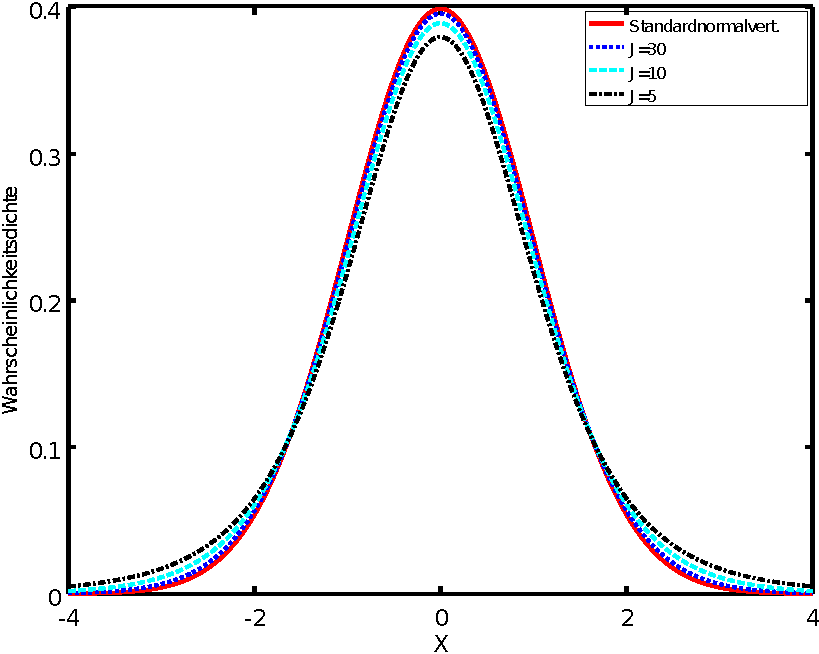
\includegraphics[width=90mm]{05_vorlesung/media/learn_Student_tpdf.pdf}
\caption{\label{studentt} \textsl{Student-t}-Verteilungen für unterschiedliche Stichprobenumfänge.}
\end{center}
\end{figure}
Um zu verdeutlichen, wie sich die Gaußverteilung und die \textsl{Student-t}-Verteilung hinsichtlich
Breite und lange Ausläufer unterscheiden, haben wir hier dies im Vergleich berechnet.
Dabei haben wir bewusst ganz extrem wenig Freiheitsgrade gewählt, nämlich nur $5$.
Wir verwenden jetzt mal den empirischen Mittelwert und die empirische Standardabweichung,
die wir aus der Gesamtheit aller Stichproben gewonnen hatten, also $y = 41.57$
und $s = 4.88$. Daraus rechnen wir sowohl die Normalverteilung als auch die
\textsl{Student-t}-Verteilung für nur fünf Freiheitsgrade und erhalten eine größere Standardabweichung
und eine größere Kurtosis aus der \textsl{Student-t}-Verteilung:
\begin{center}
\begin{tabular}{l||c|c}
\hline
Verteilung & $\sigma$ & Kurt\\
\hline
Gauß &   4.88 &  2.99 \\
Student-t &  5.86 &  3.59 \\
\hline
\end{tabular}
\end{center}
Dementsprechend sind auch die Quantile größer.


Die Kurtosis der \textsl{Student-t}-Verteilungen nimmt Werte an, die um so größer werden, je flacher die Verteilungsdichte
ist, also je ausgeprägter die \textsl{Tails} sind, also je kleiner die Stichprobenumfänge bzw.\ die
Anzahl der Freiheitsgrade sind.

%----

Das Vertrauensintervall zu einem Vertrauensniveau von $1 - \alpha$ für eine endlich große
Strichprobe mit Stichprobenumfang $J$ schätzen wir mit dem Quantil der \textsl{Student-t}-Verteilung ab.
Die Anzahl der Freiheitsgrade entspricht dem Stichprobenumfang abzüglich der Anzahl der zu
schätzenden Modellparameter, was in diesem Fall einer ist, also $\nu = J - 1$.



%---------------

Während für die Standardnormalverteilung das Quantil $z_{0.975} \; = \; 1.96$ beträgt, haben
wir aus der \textsl{Student-t}-Verteilung zu demselben Vertrauensniveau für $\nu = 50$ Freiheitsgrade
$t_{0.975, 50} \; = \; 2.01$ und für $\nu = 5$ Freiheitsgrade $t_{0.975, 5} \; = \; 2.57$.

\begin{figure}
\begin{center}
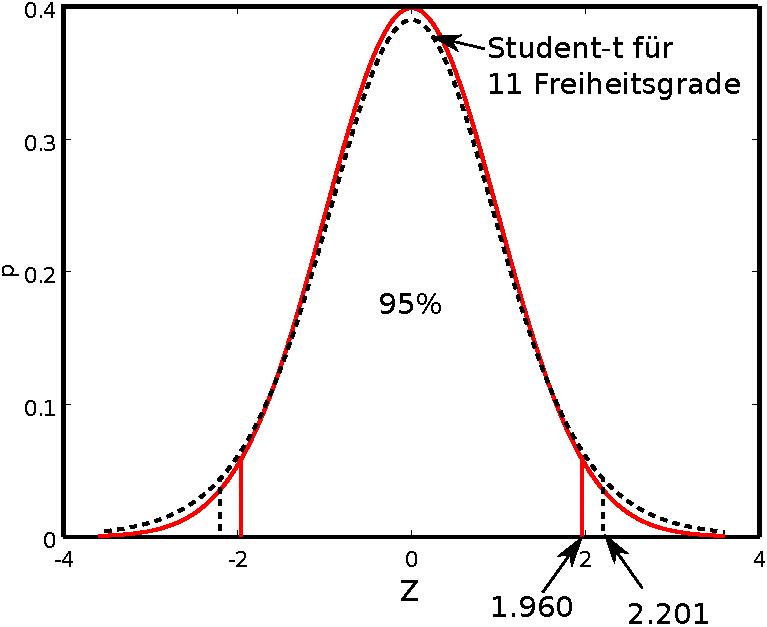
\includegraphics[width=80mm]{05_vorlesung/media/vertrauensintervall_nu_11.pdf}
\caption{\label{Vertrauensintervalle} Vertrauensintervalle in Vergleich für die
Standardnormalverteilung (rote Kurve)
und die \textsl{Student-t}-Verteilung für $\nu = 11$ Freiheitsgrade (schwarze gestrichelte Kurve).}
\end{center}
\end{figure}
Für das zweiseitige, symmetrische Intervall verwenden wir das Quantil $t_{1-\alpha/2,\nu}$, so dass
wir folgendes Vertrauensintervall erhalten:
$$
[y - t_{1-\alpha/2,\nu} s, y + t_{1-\alpha/2,\nu} s]
$$
Die Breite wird durch die Anzahl der Freiheitgrade beeinflusst, je kleiner
die Anzahl der Freiheitsgrade ist, desto breiter wird das Intervall. Die beiden Abbn.~\ref{studentt}
und \ref{Vertrauensintervalle}
zeigen, dass die \textsl{Tails} einer \textsl{Student-t}-Verteilung für wenige Freiheitsgrade
deutlich breiter sind als bei der Standardnormalverteilung, folglich auch das
Vertrauensintervall breiter ist. In Abb.~\ref{Vertrauensintervalle} sind die Quantile für
ein Vertrauensniveau von $1 - \alpha = 0.95$ eingezeichnet.

Das \textsl{(vollständige) Messergebnis} geben wir an als
Schätzwert zur Größe $Y$ gemeinsam mit dem Vertrauensintervall.
Eine gebräuchliche Schreibweise ist
\begin{equation}
Y \; = \; y \, \pm \, t_{1-\alpha/2,\nu} s .
\label{vollstaendigesErgebKlassisch}
\end{equation}

Als nächstes befassen wir uns damit, das Vertrauensintervall des Mittelwertes abzuschätzen.
Dazu betrachten wir ein Beispiel, bei dem aus einer Grundgesamtheit mit den wahren
Werten $Y = 42$ und $\sigma = 7$ mehrere Stichproben genommen werden, beispielsweise $K = 15$,
wobei jede Stichprobe einen Umfang von $J = 25$ habe. Zu jeder der Stichproben $k = 1\dots K$
berechnen wir den Mittelwert $y_k$ und die empirische Standardabweichung $s_k$.

\begin{tabular}{c||c|c|c|c|c|c|c|c}
$k$   &  1     &    2   &    3   &   4    &    5   &   6    &   7    &   8   \\
\hline\hline
$y_k$ & 41.813 & 41.854 & 39.084 & 42.117 & 41.532 & 40.428 & 42.717 & 39.727\\
\hline
$s_k$ &  6.476 &  7.706 &  6.996 &  7.729 &  6.431 &  7.516 &  7.505 &  7.439\\
\end{tabular}

\vspace{3mm}

\begin{tabular}{c||c|c|c|c|c|c|c}
$k$   &  9     &    10  &   11   &   12   &   13   &   14   &   15  \\
\hline\hline
$y_k$ & 40.858 & 39.670 & 44.351 & 42.011 & 41.935 & 44.509 & 39.921\\
\hline
$s_k$ &  8.568 &  7.649 &  6.082 &  7.661 &  7.084 &  7.878 &  7.084\\
\end{tabular}

Der Mittelwert $\bar y$ der Mittelwerte liefert dann
$$
\bar y \; = \; \frac{1}{K} \sum\limits_{k=1}^K y_k \; = \; 41.502
$$
und die empirische Standardabweichung der Mittelwerte $y_k$ liefert
$$
\bar s \; = \; \sqrt{\frac{1}{K-1} \sum\limits_{k=1}^K (y_k \, - \, \bar y)^2 }
 \; = \; 1.606
$$
Das wiederholte Ziehen von Stichproben kann für so manche Anwendung kostspielig sein,
so dass es gilt die empirische Standardabweichung des Mittelwerts aus nur einer
Stichprobe abzuschätzen.
Dazu betrachten wir die Likelihood
\begin{equation}
l(Y, \sigma | \{X_{1,1}, \dots, X_{1,J}\}) \; = \;
\prod\limits_{j=1}^J \frac{1}{\sqrt{2 \pi} \, \sigma}
 e^{- \frac{1}{2} \, \left( \frac{(X_{1,j} - Y)}{\sigma} \right)^2 }
\label{LikelihoodY}
\end{equation}
und
setzten den Schätzer $y$ der Größe $Y$ als nahrhafte Null ein
\begin{equation}
l(Y, \sigma | \{X_{1,1}, \dots, X_{1,J}\}) \; = \;
\prod\limits_{j=1}^J \frac{1}{\sqrt{2 \pi} \, \sigma}
 e^{- \frac{1}{2} \, \left( \frac{(X_{1,j} - y) - (Y - y)}{\sigma} \right)^2 }
\label{LikelihoodNahrhafteNull}
\end{equation}
d.h.
\begin{equation}
l(Y, \sigma | \{X_{1,1}, \dots, X_{1,J}\}) \; = \;
 \frac{1}{(\sqrt{2 \pi} \, \sigma)^J}
 e^{- \frac{1}{2} \, \sum\limits_{j=1}^J \left( \frac{(X_{1,j} - y) - (Y - y)}{\sigma} \right)^2 } .
\end{equation}
mit folgender Nebenrechnung für die Summe im Exponenten
$$
\arraycolsep=2.4pt\def\arraystretch{2}
\begin{array}{ll}
\sum\limits_{j=1}^J \left( (X_{1,j} - y) - (Y - y) \right)^2  & =
\sum\limits_{j=1}^J \left( (X_{1,j} - y)^2 + (Y - y)^2 - 2 (X_{1,j} - y) (Y - y) \right) \\
 & = \left( \sum\limits_{j=1}^J  (Y - y)^2\right) +
 \left( \sum\limits_{j=1}^J  (X_{1,j} - y)^2\right) - 2 \sum\limits_{j=1}^J (X_{1,j} - y) (Y - y)\\
 & = J (Y - y)^2 +
 \left( \sum\limits_{j=1}^J  (X_{1,j} - y)^2\right) = J (Y - y)^2
\end{array}
$$
und $\sum\limits_{j=1}^J (X_{1,j} - y) (Y - y) = 0$ wegen $J y = \sum\limits_{j=1}^J X_{1,j}$
gilt für die Likelihood folgende Proportionalität
\begin{equation}
l(Y, \sigma | \{X_{1,1}, \dots, X_{1,J}\}) \; \propto \;
 e^{- \frac{1}{2} \, J \, \left( \frac{(Y - y)}{\sigma} \right)^2 }
\label{LikelihoodmitJ}
\end{equation}
und wir definieren folgende Größe
\begin{equation}
\bar \sigma^2 \; := \; \frac{\sigma^2}{J}
\label{VarianzMittelwert}
\end{equation}
als \textsl{Varianz des Mittelwertes}.

Damit lässt sich Gl.~(\ref{LikelihoodmitJ}) umschreiben in
\begin{equation}
l(Y, \sigma | \{X_{1,1}, \dots, X_{1,J}\}) \; \propto \;
 e^{- \frac{1}{2} \, \left( \frac{(Y - y)}{\bar \sigma} \right)^2 } .
\end{equation}
Nun setzen wir in die Definitionsgleichung
der Varianz des Mittelwertes Gl.~(\ref{VarianzMittelwert}) bzw.\
die Wurzel daraus die empirisch ermittelten Werte unseres Beispiels ein:
\begin{equation}
\bar s \; = \; \frac{s}{\sqrt{J}}
\label{empirischeVarianzMittelwert}
\end{equation}

\begin{tabular}{c||c|c|c|c|c|c|c|c}
$k$   &  1     &    2   &    3   &   4    &    5   &   6    &   7    &   8   \\
\hline\hline
$\bar s_k$ &  1.295 &  1.541 &  1.399 &  1.546 &  1.286 &  1.503 &  1.501 &  1.488\\
\end{tabular}

\vspace{3mm}

\begin{tabular}{c||c|c|c|c|c|c|c}
$k$   &  9     &    10  &   11   &   12   &   13   &   14   &   15  \\
\hline\hline
$\bar s_k$ &  1.714 &  1.530 &  1.216 &  1.532 &  1.417 &  1.576 &  1.417\\
\end{tabular}

Jede einzelne Stichprobe liefert eine etwas unterschiedliche Abschätzung für die
Standardabweichung des Mittelwertes. Die Werte für $\bar s$ liegen mit $1.3$ bis $1.5$
knapp unter $1.6$. Es wird die Standardabweichung des Mittelwertes leicht unterschätzt, weil
der einzelne Stichprobenumfang mit $J = 25$ größer ist als die Anzahl der Stichproben mit
$K = 15$.

Das \textsl{Vertrauensintervall für die Schätzung des Mittelwertes} im Gegensatz zur
Schätzung des Einzelwertes ist damit
$$
[y - t_{1-\alpha/2,\nu} \bar s, y + t_{1-\alpha/2,\nu} \bar s]
$$
und in der Schreibweise als \textsl{vollständiges Messergebnis}
\begin{equation}
Y \; = \; y \, \pm \, t_{1-\alpha/2,\nu} \bar s .
\label{vollstaendigesErgebMittelwert}
\end{equation}


%===============


\section{\textsl{t}-Test - Mittelwerttest}


Nicht nur um die Qualität von schwarzem Bier (Stout) zu überprüfen, sondern ganz
allgemein, wird der \textsl{t}-Test eingesetzt, um zu testen, ob
\begin{enumerate}
\item eine Stichprobe zu einer Grundgesamtheit gehört,
 deren Erwartungswert bekannt ist;
\item zwei Stichproben zur gleichen Grundgesamtheit gehören,
 deren Erwartungswert nicht bekannt ist, sondern die beiden
 Mittelwerte der jeweiligen Stichproben miteinander verglichen werden.
\end{enumerate}

Die Nullhypothese $H_0$ für den Test (1.), ob der Erwartungswert $\mu_1$ einer
Stichprobe zu einer Grundgesamtheit gehört
und damit dem Erwartungswert der Grundgesamtheit, deren Erwartungswert $\mu_0$ bekannt ist,
entspricht lautet: Der Erwartungswert $\mu_1$ der Stichprobe
ist gleich dem  Erwartungswert $\mu_0$ der Grundgesamtheit, $\mu_1 = \mu_0$.
Die Alternativhypothese $H_\mathrm{a}$
lautet, dass sie einen anderen Erwartungswert hat, also $\mu_1 \neq \mu_0$,
und damit zu einer anderen Grundgesamtheit gehört.

Der Test auf Vergleich des Erwartungswerts einer Stichprobe, der Einstichproben-\textsl{t}-Test,
wird wie folgt formuliert:
\begin{center}
\begin{tabular}{c|cl}
$H_0$ & $\mu_1 = \mu_0$ & die Stichprobe hat den gleichen Erwartungswert wie die Grundgesamtheit\\
\hline
$H_\mathrm{a}$ & $\mu_1 \neq \mu_0$ & die Stichprobe hat einen anderen Erwartungswert und\\
 & & gehört somit nicht zur Grundgesamtheit
\end{tabular}
\end{center}

Die Prüfgröße ist die Differenz zwischen empirisch berechnetem Mittelwert der Stichprobe
und Erwartungswert der Grundgesamtheit normiert auf die
Standardabweichung des Mittelwerts $\bar s$ der Stichprobe. Mit $y$ für den Mittelwert der
Stichprobe ist $y = \frac{1}{J}\sum_{j=1}^J X_{1,j}$ und mit der Varianz des Mittelwerts
\begin{equation}
\bar s^2 \; = \; \frac{1}{J (J - 1)} \sum_{j=1}^{J} \, (X_{1,j} - y)^2
\end{equation}
ist die Prüfgröße des Einstichproben-\textsl{t}-Tests wie folgt definiert
\begin{equation}
T \; = \; \frac{y \, - \, \mu_0}{\bar s}
\label{tTestonesample}
\end{equation}
Die Nullhypothese wird mit einem Signifikanzniveau von $\alpha = 0.05$ abgelehnt, wenn
der Betrag der Prüfgröße größer als das entsprechende Quantil der \textsl{t}-Verteilung ist
\begin{equation}
|T| \; > \; t_{1-\frac{1}{2} \alpha, \, \nu} \qquad \Rightarrow \qquad H_0 \; \; \mathrm{ablehnen}
\end{equation}
wobei $\nu$ die Anzahl der Freiheitsgrade der Stichprobe ist, $\nu = J-1$.

Der Test (2.), ob zwei Stichproben zur gleichen Grundgesamtheit gehören,
 deren Erwartungswert nicht bekannt ist, sieht wie folgt aus:
Sei $\mu_1$ der Erwartungswert der Grundgesamtheit zu Stichprobe 1 mit
Beobachtungen $(X_{1,1},\dots,$ $X_{1,J_1})$ und sei $\mu_2$ der Erwartungswert der
zu Stichprobe 2 mit Beobachtungen $(X_{2,1}, \dots, X_{2,J_2})$.
Die Nullhypothese $H_0$ lautet, dass beide denselben Erwartungswert haben,
was soviel bedeutet wie $\mu_1 = \mu_2$. Die Alternativhypothese $H_\mathrm{a}$
lautet, dass sie unterschiedliche Erwartungswerte haben, was soviel bedeutet wie $\mu_1 \neq \mu_2$,
und damit zu unterschiedlichen Grundgesamtheiten gehören.

Umgekehrt, bedeutet aber nicht, dass wenn sie denselben Erwartungswert haben,
sie zwingend zu derselben Grundgesamtheit gehören. Das zu prüfen erfordert die
in den nachfolgenden Abschnitten behandelten Tests der Varianzen, den $\chi^2$-Test bei
Test der empirischen Varianz einer Stichprobe mit einer bekannten Varianz, den
F-Test bei Test der Varianzen zweier Stichproben.

Der Test auf Erwartungswerte, der \textsl{t}-Test, wird wie folgt formuliert:
\begin{center}
\begin{tabular}{c|cl}
$H_0$ & $\mu_1 = \mu_2$ & beide Stichproben haben den gleichen Erwartungswert\\
\hline
$H_\mathrm{a}$ & $\mu_1 \neq \mu_2$ & beide Stichproben haben unterschiedliche Erwartungswerte und\\
 & & gehören somit unterschiedlichen Grundgesamtheiten an
\end{tabular}
\end{center}

Die Prüfgröße ist die Differenz der empirisch berechneten Mittelwerte normiert auf die
Standardabweichungen der Mittelwerte. Mit Gl.~(\ref{empirischeStd}) wird die
empirische Standardabweichung einer Stichprobe berechnet. Das in Tabelle 1 aufgeführte
Beispiel zeigt, dass die Mittelwerte deutlich weniger streuen, als die Werte innerhalb
einer einzelnen Stichprobe. Die Varianz des Mittelwertes einer Stichprobe wird gemäß
Gl.~(\ref{empirischeVarianzMittelwert})
darüber abgeschätzt, dass sie durch den Stichprobenumfang geteilt wird:
\begin{equation}
\bar s_i^2 \; = \; \frac{1}{J_i (J_i - 1)} \sum_{j=1}^{J_i} \, (X_{i,j} - y_i)^2
\end{equation}
Die Prüfgröße des \textsl{t}-Tests für den Vergleich der beiden Stichproben $i = 1,2$ ist wie folgt definiert
\begin{equation}
T \; = \; \frac{y_1 \, - \, y_2}{\sqrt{\bar s_1^2 + \bar s_2^2}}
\label{tTest}
\end{equation}
mit
\begin{equation}
y_i \; = \; \frac{1}{J_i}\sum_{j=1}^{J_i} \, X_{i,j} \qquad \mathrm{mit} \qquad
i = 1, 2
\end{equation}
Die Nullhypothese wird mit einem Signifikanzniveau von $\alpha = 0.05$ abgelehnt, wenn
der Betrag der Prüfgröße größer als das entsprechende Quantil der \textsl{t}-Verteilung ist
\begin{equation}
|T| \; > \; t_{1-\frac{1}{2} \alpha, \, \nu} \qquad \Rightarrow \qquad H_0 \; \; \mathrm{ablehnen}
\end{equation}


Für den $t$-Test mit zwei Stichproben wird unterschieden nach \textsl{gepoolten} und \textsl{nicht gepoolten}
Stichproben. Unter \textsl{gepoolten} Stichproben (\textsl{Samples}) versteht man diejenigen, deren Varianzen
im wesentlichen als gleich zu betrachten sind.
Die gemeinsame Anzahl der Freiheitsgrade für \textsl{gepoolte} Samples, die für die Wahl des $t$-Quantils gebraucht wird, ist
\begin{equation}
\nu \; = \; J_1 + J_2 - 2
\label{dofpooled}
\end{equation}
und für NICHT \textsl{gepoolte}
\begin{equation}
\nu \; = \;
 \frac{ \left(\frac{s_1^2}{J_1} +\frac{s_2^2}{J_2}\right)^2}{
  \frac{\left(\frac{s_1^2}{J_1}\right)^2}{J_1 - 1} + \frac{\left(\frac{s_2^2}{J_2}\right)^2}{J_2 - 1} } .
\label{dofnonpooled}
\end{equation}
Die Herleitung zur Berechnung der Anzahl der Freiheitsgrade für nicht gepoolte Stichproben
wird in Kapitel \ref{unsicherheitsfortpfLin} dran kommen. Gl.~(\ref{dofnonpooled}) wird auch
Satterthwaite'sche Gleichung genannt.

Bei $\nu = J_1 + J_2 - 2$ Freiheitsgraden, bei dem hier betrachteten Beispiel ist dies
$\nu = 98$ und $t_{1-\frac{1}{2} \alpha, \, \nu} = t_{0.975, 98} = 1.985$.
Der Vergleich der ersten mit der zweiten Stichprobe aus Tabelle 1 liefert
$$
|T| \; = \; \frac{|40.79 \; - \; 43.08|}{\sqrt{\frac{1}{50} (4.83)^2 \; + \; \frac{1}{50} (5.52)^2}}
\; = \; 2.21  \; > \; 1.99
$$
dass die Mittelwerte der beiden Stichproben signifikant, auf einem Signifikanzniveau von
$\alpha = 0.05$, von einander abweichen und die Nullhypothese verworfen wird.

Betrachtet man jedoch einen größeren Vertrauensbereich, also anstelle von $95 \%$ einen
Bereich von $98 \%$, nimmt man also mehr aus dem Bereich der \textsl{Tails} hinzu, so
wird die Nullhypothese nicht verworfen. Auf einem Signifikanzniveau von nur
$\alpha = 0.02$ hat das Vertrauensintervall die Grenzen
$-t_{1-\frac{1}{2} \alpha, \, \nu} = -t_{0.99, 98} = -2.365$ und
$t_{1-\frac{1}{2} \alpha, \, \nu} = t_{0.99, 98} = 2.365$. Die
Nullhypothese wird für diese Wahl des Signifikanzniveaus nicht verworfen,
weil die Prüfgröße innerhalb des breiteren Intervalls mit
$|T| \; = \; 2.21 \; < \; 2.37$ liegt.

\begin{verbatim}
http://www.itl.nist.gov/div898/handbook/eda/section3/eda353.htm
\end{verbatim}

\section{$\chi^2$-Verteilung und Test einer Varianz}


Eine Verteilungsdichtefunktion, die die Verteilung der Quadrate einer
 normierten Zufallsgröße $Z$,
also die Verteilung der Varianzen einer Zufallsgröße $X$, beschreibt, ist die
$\chi^2$-Verteilung, gesprochen \textsl{Chi-Quadrat}-Verteilung.


Bisher haben wir uns damit befasst, wie eine Zufallsgröße $X$ streut.
Jetzt betrachten wir, wie die Streuung ihrerseits streut.
Wir betrachten eine Zufallsgröße, die zu einer normalverteilten Grundgesamtheit gehört.
\begin{quote}
$X$ sei eine eine normalverteilte Zufallsgröße mit Erwartungswert $\mu$ und Varianz $\sigma^2$
\end{quote}
d.h.
\begin{equation}
X \; \sim \; \mathcal{N}(\mu, \sigma).
\end{equation}
Werden einzelne kleinere Stichproben $X_i$ aus der Grundgesamtheit von $X$ entnommen, die
jeweils einen Stichprobenumfang $J_i$ haben und werden die jeweiligen Mittelwerte und
empirischen Varianzen berechnet
\begin{equation}
y_i \; = \; \frac{1}{J_i} \, \sum_{j=1}^{J_i} \, X_{i,j} \qquad
 s_i^2 \; = \; \frac{1}{J_i-1} \, \sum_{j=1}^{J_i} \, (X_{i,j} \, - \, y_i)^2
\end{equation}
so haben wir anhand der zuvor behandelten Beispiele festgestellt,
dass nicht nur die Mittelwerte $y_i$ sondern auch die Varianzen $s_i^2$ streuen.
Die Charakteristik der Verteilungsdichte der Varianzen hängt vom
Stichprobenumfang $J_i$ ab. Der Stichprobenumfang entspricht der Anzahl der Freiheitsgrade.

Gegeben sei eine Stichprobe $Z_1, \dots, Z_J$ unabhängiger Beobachtungen einer
standardnormalverteilten Zufallsgröße $Z  \sim \; \mathcal{N}(0, 1)$:
Dann ist die Summe der Quadrate der Beobachtungen $Q$
\begin{equation}
Q \; = \; \sum_{j=1}^J \, Z_j^2
\end{equation}
gemäß folgender Wahrscheinlichkeitsdichtefunktion verteilt
\begin{equation}
p_\mathrm{\chi^2}(Q, \nu) \; = \; \frac{Q^{\frac{\nu}{2} - 1} \,
 e^{-\frac{Q}{2}}}{2^{\frac{\nu}{2}} \, \Gamma(\frac{\nu}{2})} \qquad Q > 0
\label{Chi2pdf}
\end{equation}
mit $\nu$ für die Anzahl der Freiheitsgrade und $\Gamma$ für die
im Abschnitt zuvor als Gl.~(\ref{GammaHalfInt}) angegebenen Gammafunktion.

Eine Schreibweise für die Aussage
\begin{quote}
$Q$ ist $\chi^2$-verteilt
\end{quote}
ist
\begin{equation}
Q \; \sim \; \chi^2(\nu).
\label{Chi2verteilt}
\end{equation}
Die Definition der $\chi^2$-Verteilungsdichtefunktion braucht nicht auswendig gelernt zu
werden. Der Umgang mit den Quantiltabellen ist aber zu üben.
Wichtig zu wissen ist, dass die $\chi^2$-Verteilungs\-dichte\-funktion für
einen positiven Wertebereich gilt, sie ihr Maximum in der Nähe von $Q = J$ hat, sie um so
schiefer und breiter ist, je kleiner $J$ ist und die Verteilungsdichte der Varianzen
\begin{equation}
s_{\mu,i}^2 \; = \; \frac{1}{J_i} \, \sum_{j=1}^{J_i} \, (X_{i,j} \, - \, \mu)^2
\end{equation}
\begin{equation}
s_{\mu}^2 \; = \; \frac{1}{J} Q \, \sigma^2  \qquad \Leftrightarrow \qquad
Q \; = \; J \, \left( \frac{s_{\mu}}{\sigma} \right)^2
\label{s2Q}
\end{equation}
liefert. Was in der Praxis hinsichtlich des Statistiktests, dem $\chi^2$-Test, gebraucht wird,
ist das Verständnis wie die Tabellen verwendet werden
und für Methoden der bayesischen Statistik erforderlichenfalls auch wie die
Funktionen der jeweils eingesetzten Numerik-/Statistik\-biblio\-theken zu benutzen sind.

\begin{figure}
\begin{center}
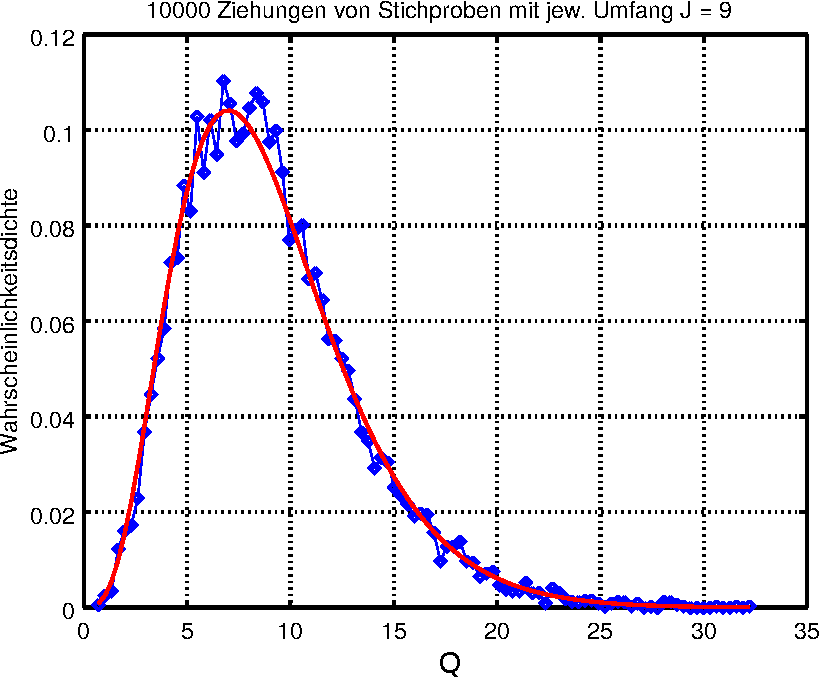
\includegraphics[width=75mm]{05_vorlesung/media/understandchi2_df9_final.pdf} \hspace{5mm}
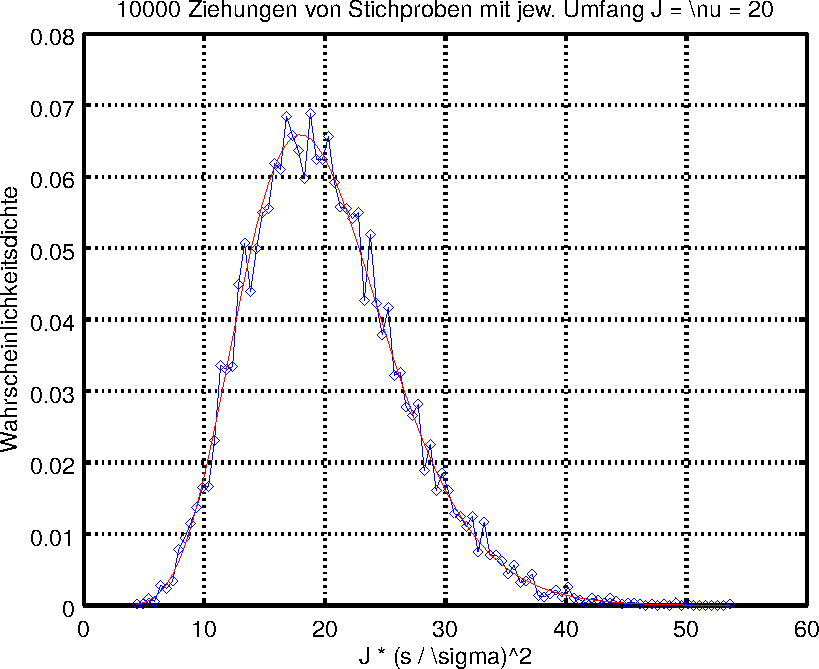
\includegraphics[width=75mm]{05_vorlesung/media/understandchi2_df20_final.pdf}
\caption{\label{ch2beispiele}$\chi^2$-Verteilung der normierten
Zufallsgröße $Q \; = \; J \, \left( \frac{s_{\mu}}{\sigma} \right)^2$ für
$s_{\mu}^2 \; = \; \frac{1}{J} \, \sum_{j=1}^{J} \, (X_{..,j} \, - \, \mu)^2$
für $J = 9$  (\textsl{links}) und $J = 20$ (\textsl{rechts}).}
\end{center}
\end{figure}

Abb.~\ref{ch2beispiele} zeigt zwei Beispiele für die Verteilungsdichte der Varianzen, zum einen
für $J = 9$ und zum anderen für $J = 20$. Mit
%\lstset{language=Matlab}
\begin{lstlisting}[style=Matlab]
function understandchi2()
  Jz = 9;
  nbin = 100;
  n = 10000;
  d = zeros(n,1);
  for k=1:n
    x = randn(Jz,1);
    d(k) = sum(x.^2);
  end
  [haeuf, bin] = hist(d,nbin);
  Deltabin = bin(2)-bin(1);
  figure(1000);
  plot(bin,haeuf/(n*Deltabin),'bd-',bin,chi2pdf(bin,Jz),'r-');
  xlabel('J * (s / \sigma)^2', 'fontsize', 14);
  ylabel('Wahrscheinlichkeitsdichte', 'fontsize', 14);
  title([num2str(n) 'Stichprobenumfang J = \nu = ' num2str(Jz)], 'fontsize', 14);
  grid on;
  set(gca, 'fontsize', 14, 'linewidth', 2);
  print(1000,['understandchi2_df' num2str(Jz) '_solid.svg'],'-dsvg');
end
\end{lstlisting}
wurden die Diagramme erzeugt. Die Verteilung der Grundgesamtheit ist die
Standardnormalverteilung mit $\mu = 0$ und $\sigma = 1$.
Eine Stichprobenentnahme wird mit \texttt{x = randn(Jz,1);} simuliert.

Wie bei der Quantildefinition für die Standardnormalverteilung und für die $t$-Verteilung
ist das Quantil der $\chi^2$-Verteilung die obere Integrationsgrenze
zur Gewinnung des Flächeninhalts der Verteilungsdichte. Dies quantifiziert die Wahrscheinlichkeit,
mit der für die Größe $Q$ Werte beobachtet werden, die kleiner sind als das Quantil.
Hier ist die untere Integrationsgrenze Null und nicht minus Unendlich, weil $Q$ per
Definitionem nur positive Werte haben kann, siehe Abb.~\ref{chi2quantil}.
\begin{figure}
\begin{center}
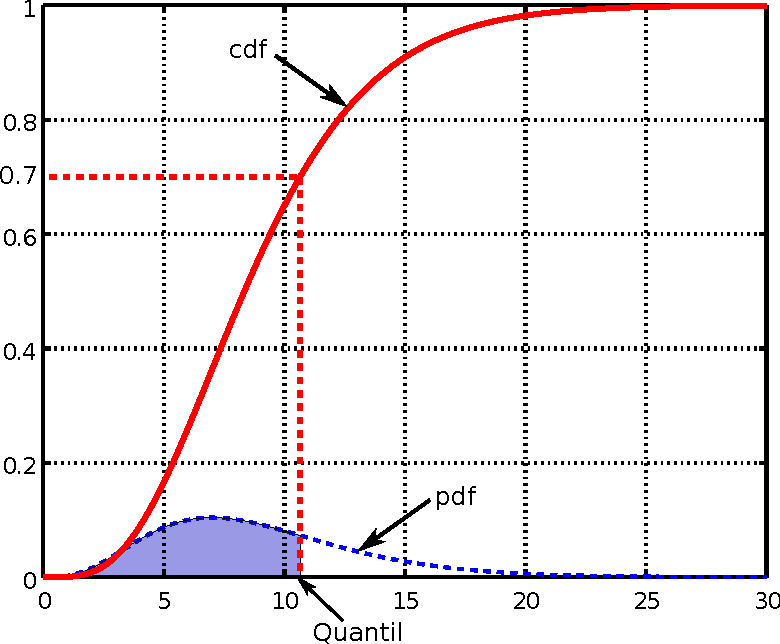
\includegraphics[width=100mm]{05_vorlesung/media/chiquadrat.pdf}
\caption{\label{chi2quantil}Wahrscheinlichkeitsverteilungsdichte (pdf) und
kumulierte Wahrscheinlichkeitsfunktion (cdf)
der normierten Varianzen, das Quantil wird $\chi^2$ genannt. Hier für
$\nu = 9$ Freiheitgrade und $1 - \alpha = 0.7$, somit $\chi^2_{\nu, 1-\alpha} = 10.66$
dargestellt.}
\end{center}
\end{figure}
\begin{equation}
P(Q) \; = \;
\int \limits_0^{\chi^2_{1-\alpha, \nu}}
p(Q^\prime, \nu) \; \operatorname{d} Q^\prime \; = \;
1 \, - \, \alpha
\label{chiQuadratQuantil}
\end{equation}
Bei dem $\chi^2$-Test wird die empirische Varianz einer Stichprobe
\begin{equation}
s_{\mu,i}^2 \; = \; \frac{1}{J_i} \, \sum_{j=1}^{J_i} \, (X_{i,j} \, - \, \mu)^2
\; \approx \; \frac{1}{J_i-1} \, \sum_{j=1}^{J_i} \, (X_{i,j} \, - \, y_i)^2
\; = \; s_i^2
\end{equation}
mit der bekannten Varianz einer Grundgesamtheit verglichen.
\begin{lstlisting}[style=Matlab]
  for k=1:n
    x = randn(Jz,1);
    y = mean(x);
    d(k) = sum((x-y).^2);
  end
\end{lstlisting}
Dann ist die Anzahl der Freiheitsgrade $\nu = J-1$ um einen vermindert,
weil der Mittelwert $y_i$ von den Werten $X_{i,j}$ abhängt. Die $\chi^2$-Verteilung
ist mit der Anzahl der Freiheitsgrade und nicht mit dem Stichprobenumfang zu verwenden
\begin{equation}
s^2 \; = \; \frac{1}{\nu} Q \, \sigma^2  \qquad \Leftrightarrow \qquad
Q \; = \; \nu \, \left( \frac{s}{\sigma} \right)^2 ,
\label{s2Qempir}
\end{equation}
so dass die $\chi^2$-Verteilungsdichte  für $\nu = J-1$ zu verwenden ist,
in Gnu-Octave beispielsweise mit dem Funktionsaufruf
\texttt{chi2pdf}:

\begin{lstlisting}[style=Matlab]
  [haeuf, bin] = hist(d,nbin);
  Deltabin = bin(2)-bin(1);
  plot(bin,haeuf/(n*Deltabin),'bd-',bin,chi2pdf(bin,Jz-1),'r-');
  xlabel('(J-1) * (s / \sigma)^2', 'fontsize', 14);
\end{lstlisting}

Beim $\chi^2$-Test wird geprüft, ob die Varianz einer Stichprobe gleich einer
spezifizierten Varianz $\sigma_0^2$ ist. Wir formulieren die Hypothesen
\begin{center}
\begin{tabular}{c|cl}
$H_0$ & $\sigma^2 = \sigma_0^2$ & die Stichprobe gehört zu einer Grundgesamtheit mit der Varianz $\sigma_0^2$\\
\hline
$H_\mathrm{a}$ & $\sigma^2 \neq \sigma_0^2$ & die Stichprobe gehört nicht zu einer Grundgesamtheit mit der Varianz $\sigma_0^2$
\end{tabular}
\end{center}
Die Testgröße ist
\begin{equation}
T \; = \; \nu \, \left( \frac{s}{\sigma_0} \right)^2 .
\label{chi2testgroesse}
\end{equation}
Die Nullhypothese wird mit einem Signifikanzniveau von $\alpha$
verworfen, falls die Testgröße außerhalb des Intervalls liegt,
das durch die in Gl.~(\ref{chiQuadratQuantil}) definierten Quantile begrenzt wird, d.h.
\begin{equation}
T \; < \; \chi^2_{\alpha/2, \nu}  \qquad \mathrm{oder} \qquad
T \; > \; \chi^2_{1-\alpha/2, \nu} .
\end{equation}
Es ist zu beachten, dass beim zweiseitigen Test für jede Seite die
Hälfte des Signifikanzniveaus verwendet wird, also $\alpha/2$.

\begin{verbatim}
http://www.itl.nist.gov/div898/handbook/eda/section3/eda358.htm
\end{verbatim}


\section{Fisherverteilung und Vergleich zweier empirischer Varianzen}

Der Fall, bei dem zu überprüfen ist, ob die Varianzen zweier Stichproben zur gleichen
Grundgesamtheit gehören müssten, bzw.\ ob diese im wesentlichen übereinstimmen, wird
als Hypothesentest wie folgt formuliert:
\begin{center}
\begin{tabular}{c|cl}
$H_0$ & $\sigma_1^2 = \sigma_2^2$ & die beiden Stichproben haben die gleichen Varianzen\\
\hline
$H_\mathrm{a}$ & $\sigma_1^2 \neq \sigma_2^2$ & die Stichproben haben unterschiedliche Varianzen
und \\
 &  & gehören somit zu unterschiedlichen Grundgesamtheiten
\end{tabular}
\end{center}
Die Testgröße ist
\begin{equation}
T \; = \; \left( \frac{s_1}{s_2} \right)^2.
\label{Ftestgroesse}
\end{equation}
Sie wird verglichen mit den beiden Quantilen, dem linksseitigen und dem rechtsseitigen, der Fisherverteilung.
Der Test wird in der Literatur Fisher-Test oder kurz F-Test genannt.

Die Fisherverteilung ist die Marginalverteilung des Produkts der Wahrscheinlichkeitsdichtefunktionen zweier
$\chi^2$-verteilter Zufallsgrößen $Q_1$ und $Q_2$
\begin{equation}
p_\mathrm{F}(R, \nu_1, \nu_2) \; = \; \int\limits_0^{\infty}
p_\mathrm{\chi^2}(R, \nu_1) \, p_\mathrm{\chi^2}(Q_2, \nu_2) \; \frac{\nu_1}{\nu_2} Q_2 \;
\mathrm{d} Q_2
\label{FisherverteilungAnsatz}
\end{equation}
mit
\begin{equation}
R  \; = \; \frac{\frac{1}{\nu_1} Q_1}{\frac{1}{\nu_2} Q_2} .
\label{TrafoQ1Q2}
\end{equation}
Dabei ist der Faktor $\frac{\nu_1}{\nu_2} Q_2$
die Funktionaldeterminante aus der Transformation $(Q_1, Q_2) \rightarrow (R, Q_2)$,
um aus der Wahrscheinlichkeitsdichtefunktion der beiden $\chi^2$-verteilten Zufallszahlen
$$
p_\mathrm{\chi^2}(Q_1, \nu_1) \, p_\mathrm{\chi^2}(Q_2, \nu_2)
$$
die Fisherverteilung zu berechnen. Nach Einsetzen der Gleichung für
die $\chi^2$-Verteilung, Gl.~(\ref{Chi2pdf}), und Ausführen der Integration
in Gl.~(\ref{FisherverteilungAnsatz}), sieht die Fisherverteilung wie folgt aus
\begin{equation}
p_\mathrm{F}(R, \nu_1, \nu_2) \; = \;
\nu_1^{\frac{\nu_1}{2}} \nu_2^{\frac{\nu_2}{2}} \,
\frac{\Gamma\left(\frac{\nu_1+\nu_1}{2}\right)}
{\Gamma\left(\frac{\nu_1}{2}\right)\Gamma\left(\frac{\nu_2}{2}\right)}
\frac{R^{\frac{\nu_1}{2}-1}}{\left(\nu_1 R + \nu_2 \right)^\frac{\nu_1+\nu_1}{2}} .
\label{Fisherpdf}
\end{equation}
Abb.~\ref{Fverteilbeispiel} zeigt beispielhaft zwei Fisherverteilungen, die mit
blau gestrichelter Kurve dargestellte für $\nu_1 = 8$ und $\nu_2 = 19$ und die mit
schwarz durchgezogener Kurve für $\nu_1 = \nu_2 = 8$ Freiheitsgrade.

\begin{figure}
\begin{center}
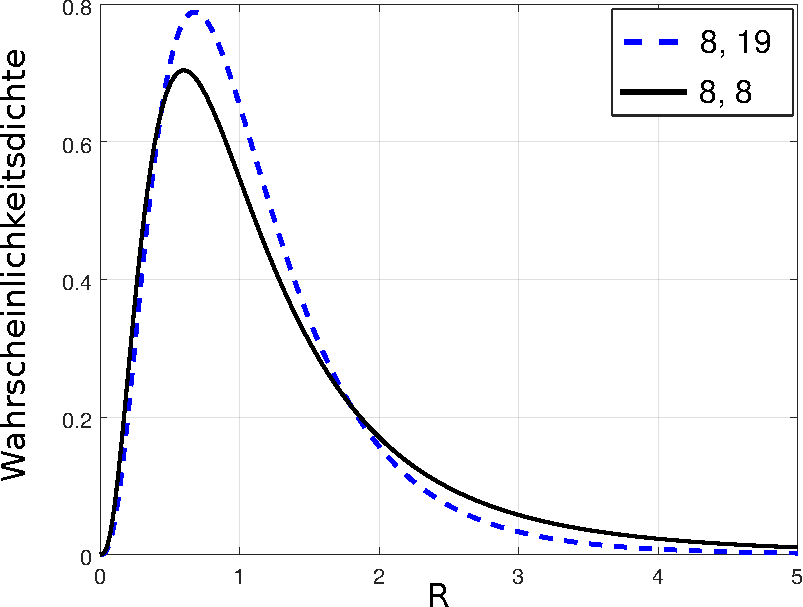
\includegraphics[width=75mm]{05_vorlesung/media/BeispielFverteilung.pdf}
\caption{\label{Fverteilbeispiel}Fisherverteilung des Quotienten $R$
zweier $\chi^2$-verteilter Zufallsgrößen $Q_1$ und $Q_2$, also
$R \; = \; \frac{\frac{1}{\nu_1} Q_1}{\frac{1}{\nu_2} Q_2} \;
= \; \frac{s_1^2}{s_2^2}$ mit jeweils der Anzahl der Freiheitsgrade
$\nu_1$ und $\nu_2$. Die beiden Kurven zeigen zwei Beispiele, die
blau gestrichelte für $\nu_1 = 8$ und $\nu_2 = 19$ und die schwarze durchgezogene
für $\nu_1 = \nu_2 = 8$ Freiheitsgrade.}
\end{center}
\end{figure}



Die Nullhypothese wird mit einem Signifikanzniveau von $\alpha$
verworfen, falls die Testgröße außerhalb des Intervalls liegt,
das durch die Quantile der Fisherverteilung begrenzt wird, d.h.
\begin{equation}
T \; < \; F_{\alpha/2, \nu_2, \nu_1}  \qquad \mathrm{oder} \qquad
T \; > \; F_{1-\alpha/2, \nu_2, \nu_1} .
\end{equation}
Dabei ist $\nu_1$ die Anzahl der Freiheitsgrade zu $s_1$, die
im Zähler stehende Standardabweichung
aber in den Tabellen Nennerfreiheitsgrad genannt wird, und $\nu_2$
die Anzahl der Freiheitsgrade zu $s_2$, die im Nenner stehende
Standardabweichung deren Freiheitsgrad
aber in den Tabellen Zählerfreiheitsgrad genannt wird. Das kommt
daher, dass in Gl.~(\ref{TrafoQ1Q2}) die Freiheitsgrade $\nu_1$ zur
Zufallsgröße $Q_1$ im Nenner stehen.

Beispiel:
Der \textsl{General Social Survey (GSS)} hatte in den USA im Jahr 2000 anhand einer
zufallsgenerierten Teilstichprobe mit $J = 652$ Erwachsenen Menschen untersucht,
wie sich die Nutzungsdauer $t$ in Stunden/Woche der Internetnutzung nach Geschlecht unterscheidet.

\begin{center}
\begin{tabular}{l|ccc}
Geschlecht & $J_i$ & $t_i$ & $s_i$\\
\hline\hline
männlich & $305$ & $5.48$ & $7.80$\\
\hline
weiblich & $347$ & $3.84$ & $5.86$
\end{tabular}
\end{center}

mit $J_i$ für die Stichprobenumfänge und $s_i$ für die Standardabweichung mit $i = 1,2$.
Die Standardabweichung zur Nutzungsdauer $t$ beträgt bei den Männern $t_1 = 5.48$  Stunden/Woche
mit einer Streuung von
$s_1 = 7.80$ Stunden/Woche und bei den Frauen
$t_1 = 3.84$  Stunden/Woche mit einer Streuung von $s_2 = 5.86$ Stunden/Woche.
Der F-Test überprüft, ob der Unterschied der Varianzen $s_1^2$ und $s_2^2$ signifikant ist.
Im vorliegenden Beispiel beträgt der Nennerfreiheitsgrad $\nu_1 = J_1 - 1 = 305-1 = 304$ und der
Zählerfreiheitsgrad $\nu_2 = J_2 - 1 = 347-1 = 346$.

\begin{lstlisting}[style=Python]
import numpy as np
import scipy.stats
alpha = 0.05
s1 = 7.80
s2 = 5.86
J1 = 305
J2 = 347
nu1 = J1-1
nu2 = J2-1
Tpruef = (s1/s2)**2
nuZaehl = nu2
nuNenn = nu1
Flinks = scipy.stats.f.ppf(alpha/2, nuZaehl, nuNenn)
Frechts = scipy.stats.f.ppf(1-alpha/2, nuZaehl, nuNenn)
print(Flinks, Tpruef, Frechts)
\end{lstlisting}
$T = 1.772$ und $F_{\alpha/2, \nu_2, \nu_1} = 0.805$ und
$F_{1-\alpha/2, \nu_2, \nu_1} = 1.245$. Mit $T = 1.772 \; > \; F_{1-\alpha/2, \nu_2, \nu_1} = 1.245$
liegt die Prüfgröße signifikant höher als das rechte Quantil.
Es kann also davon ausgegangen werden, dass sich die Varianzen der beiden Geschlechter signifikant voneinander unterscheiden.

\section{Anwendung von Hypothesentests}

Anwendung finden die Hypothesentests im Bereich der Qualitätssicherung in der Produktion (siehe beispielsweise
zur Prüfung des Stout in der Guinnessbrauerei schon vor 100 Jahren), oder im Bereich der Naturwissenschaften
(Biologie, Chemie, Pharmazie, Medizien) zum Nachweis von Substanzen. Es geht darum, dass zu bewerten ist,
mit welcher Wahrscheinlichkeit Beobachtungen zu welcher Verteilung gehören.
Einer Entscheidung liegen Regeln zugrunde. Mit dem $t$-Test haben wir die Regeln kennengelernt, über
die wir entscheiden, ob zwei Datensätze den gleichen Erwartungswert haben.

Als nächstes wollen wir untersuchen, welche Fehler mit welcher Wahrscheinlichkeit dabei entstehen können.
Anschließend wollen wir uns ansehen, wie eine Stichprobe mit einer Toleranzvorgabe verglichen wird.
Die Toleranzvorgabe liefert ein Intervall, dessen Lage mit der Lage der Wahrscheinlichkeitsverteilung
der zu untersuchenden Stichprobe verglichen wird.

\subsection{Entscheidung bei Vergleich zweier Stichproben}
\begin{figure}
\begin{center}
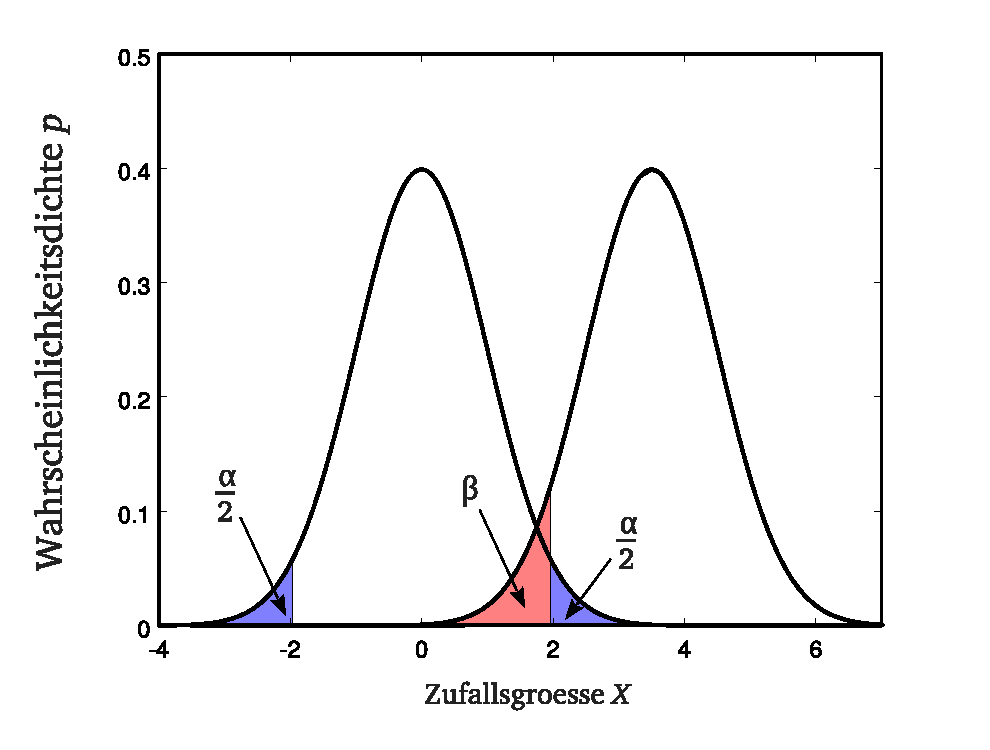
\includegraphics[width=100mm]{05_vorlesung/media/entscheidungsfehlertypen.pdf}
\caption{\label{entscheidungsfehler} Die Ereignisse (beobachtete Werte) aus der linken Wahrscheinlichkeitsdichteverteilung,
 die in deren \textsl{Tails} liegen, werden mit einem Signifikanzniveau von $\alpha$ verworfen.
 Die Ereignisse (beobachtete Werte) aus der rechten Wahrscheinlichkeitsdichteverteilung, die in dessen linkem
 \textsl{Tail} liegen, werden mit Wahrscheinlichkeit $\beta$ als der linken Wahrscheinlichkeit zugehörig
 erachtet.}
\end{center}
\end{figure}
Den Hypothesentests, die wir uns angesehen haben, ist gemeinsam, dass
\begin{enumerate}
\item eine Nullhypothese $H_0$ (evtl.\ auch eine Alternativhypothese $H_\mathrm{a}$)
aufgestellt wurde,
\item ein Signifikanzniveau $\alpha$ spezifiziert wurde,
\item eine Stichprobe mit einer Anzahl Freiheitsgrade $\nu$
genommen wurde und
\item anhand der vorher aufgestellten Entscheidungsregeln (Vergleich einer
Prüfgröße mit dem Quantil einer Wahrscheinlichkeitsdichteverteilung)
die Hypothese verworfen oder angenommen wurde.
\end{enumerate}
In der Entscheidungsregel werden durch Vorgabe eines Signifikanzniveaus Verwerfungsbereich
und Annahmebereich festgelegt. Das Signifikanzniveau ist dabei Komplementärwahrscheinlichkeit
(Gegenwahrscheinlichkeit) zum Vertrauensniveau, das ist die Wahrscheinlichkeit dafür
wie sicher die Hypothese ist.

Die Wahrscheinlichkeit, mit einem Hypothesentest eine falsche
Entscheidung zu treffen wird in zwei Klassen von Fehlern aufgeteilt, den
$\alpha$-Fehler oder den $\beta$-Fehler

\begin{center}
\begin{tabular}{M{3cm}|M{5.5cm}|M{5.5cm} N}
                 &     $H_0$ annehmen    &     $H_0$ ablehnen   \\[3pt]
\hline
$H_0$ ist wahr   & richtige Entscheidung, Wahrscheinlichkeit: $1-\alpha$ & Fehler 1.\ Art, Wahrscheinlichkeit $\alpha$ \\[3pt]
\hline
$H_0$ ist falsch & Fehler 2.\ Art, Wahrscheinlichkeit: $\beta$  & richtige Entscheidung, Wahrscheinlichkeit: $1-\beta$
\end{tabular}
\end{center}

Abb.~\ref{entscheidungsfehler} soll illustrieren, dass Beobachtungswerte, die zu einer
Grundgesamtheit mit einer Wahrscheinlichkeitsdichteverteilung mit Erwartungswert
$\mu_\mathrm{a} = 3.5$ gehören, per Hypothesentest einer Grundgesamtheit mit $\mu_0 = 0$
zugeordnet werden. Die Wahrscheinlichkeit für das Auftreten solcher Beobachtungen ist
dann $\beta$. Das Diagramm wurde mit folgendem Octaveskript erzeugt

\begin{lstlisting}[style=Matlab]
function plot_entscheidungsfehler()
  dz = 0.02;
  lim = 7;
  z = [-lim:dz:lim];
  p1 = normpdf(z,0,1);
  t = 1.96;
  zleft = [-lim:dz:-t];
  pleft = normpdf(zleft,0,1);
  zright = [t:dz:lim];
  pright = normpdf(zright,0,1);
  mu2 = 3.5;
  p2 = normpdf(z+mu2,mu2,1);
  zbeta = [mu2-lim:dz:t];
  pbeta = normpdf(zbeta,mu2,1);
  figure(200); hold on;
  area( zleft, pleft, 'Facecolor', [0.5 0.5 1]);
  area( zright, pright, 'Facecolor', [0.5 0.5 1]);
  area( zbeta, pbeta, 'Facecolor', [1 0.5 0.5]);
  plot( z, p1, 'k-', 'linewidth', 2);
  plot( z+mu2, p2, 'k--', 'linewidth', 2);
  xlabel('X', 'fontsize', 14);
  ylabel('p', 'fontsize', 14);
  axis([-4 7 0 0.5]);
  set(gca, 'fontsize', 14);
  hold off;
  print(200, 'entscheidungsfehler.svg', '-dsvg');
end
\end{lstlisting}

\subsection{Konformitätsprüfung}
Nachdem wir gesehen haben wie wir zwei Hypothesen über die Lage zweier Wahrscheinlich\-keits\-dichte\-ver\-teilungen
verglichen haben, befassen wir uns jetzt mit dem Vergleich von Grenzen, den Toleranzgrenzen, mit einer
Wahrscheinlichkeitsdichteverteilung. Für die Fertigung werden in den Konstruktionszeichnungen zu den Merkmalen
von Bauteilen die Toleranzgrenzen eingetragen, innerhalb derer die Merkmale des Werkstücks liegen müssen. Wie nun
bewertet man nach Fertigstellung des Werkstücks, ob ein Merkmal innerhalb einer Toleranzvorgabe liegt? Ein Merkmal
wird durch einen Messvorgang geprüft. Der Messvorgang liefert ein Ergebnis: Einen Zahlenwert für das Merkmal und
ein Überdeckungsintervall zusammen mit einem Vertrauensniveau. Anstelle von Überdeckungsintervall und Vertrauensniveau
kann auch direkt eine Wahrscheinlichkeitsdichteverteilung angegeben werden, ist aber sehr unüblich in der industriellen
Praxis. Für die Bewertung, ob das gefertigte Werkstück mit der Vorgabe der Konstruktion übereinstimmt, ob es konform ist,
werden Messergebnis und Toleranzvorgabe verglichen.

Als Ergänzung (\textsl{Supplement}) zum \glqq Guide of Uncertainty\grqq ~gibt es das Dokument
\textsl{Evaluation of measurement data - The role of measurement uncertainty in conformity assessment},
das darlegt, wie Konformitätsbewertungen vorzunehem sind.
\begin{verbatim}
https://www.bipm.org/utils/common/documents/jcgm/JCGM_106_2012_E.pdf
\end{verbatim}
Dort heißt es in Paragraph 7.1.1
\begin{quote}
An item conforms to a specified requirement,
if the true value of its associated property $Y$ lies in the tolerance
interval. Knowledge of $Y$ is conveyed by a probability density function $p(y|{X_1,\dots,X_J})$
so that a statement of conformity is always an inference,
with some probability of being true. Denoting the set of permissible (conforming) values
$Y$ by $C$, the conformance probability, denoted by $p_\mathrm{c}$, is given by
\begin{equation}
	p_\mathrm{c} = P(Y \in C | {X_1,\dots,X_J}) = \int\limits_C p(y|{X_1,\dots,X_J}) \mathrm{d}y.
\end{equation}
\end{quote}
Im Originaldokument werden Sie eine etwas andere Schreibweise für die Bezeichner in der Formel vorfinden.
Hier ist es so aufgeschrieben, wie es zu der Notation innerhalb dieses Vorlesungsskriptes, insbesondere
zu Kapitel \ref{KonzepteinverseProbleme}, passt.
Für die Toleranz wird in der Richtlinie zur Konformitätsbewertung zur Wahrung der Allgemeingültigkeit
eine Menge $C$ angegeben. Falls die Größe $Y$ eine skalarwertige Größe wie bei dem Beispiel, anhand dessen
wir in Kapitel \ref{KonzepteinverseProbleme} das Prinzip der bayesischen Statistik illustriert haben,
so steht $C$ für ein Intervall $C = [T_\mathrm{L}, T_\mathrm{U}]$ im Falle der zweiseitigen
Grenzen, $C = [-\infty, T_\mathrm{U}]$ für den Fall, dass es eine Obergrenze gibt,
$C = [T_\mathrm{L}, \infty]$, dass es eine Untergrenze gibt. Dabei sollen der Index L für \glqq lower
limit\grqq ~und der Index U für \glqq upper limit\grqq ~stehen. Der Bezeichner $T$ ist in der
Normung das üblicherweise für Toleranzgrenzen verwendete Symbol und bedeutet an dieser
Stelle nicht Testgröße! Er unterscheidet sich von den Testgrößen durch seine Indizes.

Die Wahrscheinlichkeit $p_\mathrm{c}$, dass die Beobachtungen ${X_1,\dots,X_J}$ innerhalb des Toleranzintervalls
$C = [T_\mathrm{L}, T_\mathrm{U}]$ liegen, ist
\begin{equation}
	p_\mathrm{c} =  \int\limits_{T_\mathrm{L}}^{T_\mathrm{U}} p(y|{X_1,\dots,X_J}) \mathrm{d}y.
\end{equation}
Für den Fall, dass von einer normalverteilten Stichprobe ausgegangen werden kann und dass eine Einzelgröße
vorliegt, wird auch der Stichprobe ${X_1,\dots,X_J}$ der Schätzer $\bar y$ aus einfacher Mittelwertbildung
gewonnen ($\bar y = \frac{1}{J} \sum\limits_{j=1}^J X_j$) und die Varianz als empirische Varianz $s$ aus
$s = \frac{1}{J-1}\sum\limits_{j=1}^J (X_j - \bar y)^2$ berechnet
und für die Wahrscheinlichkeitsdichte $p$ die Gaußverteilung verwendet
\begin{equation}
	p_\mathrm{c} = \frac{1}{\sqrt{2 \pi} s} \int\limits_{T_\mathrm{L}}^{T_\mathrm{U}}
	e^{-\frac{1}{2}\left(\frac{y - \bar y}{s}\right)^2} \mathrm{d}y .
\end{equation}
Die Größe $\frac{y - \bar y}{s}$ ist eine normierte Zufallsgröße. Die Integrationsgrenzen können gleichfalls
normiert werden: $z = \frac{y - \bar y}{s}$, $z_\mathrm{L} = \frac{y_\mathrm{L} - \bar y}{s}$ und
$z_\mathrm{U} = \frac{y_\mathrm{U} - \bar y}{s}$, so dass die Tabellenwerke für die kumulative
standardnormalverteilte Gaußfunktion oder die Bibliotheksfunktion
für die gauß'sche Fehlerfunktion (\textsl{error function}) wie folgt verwendet werden kann:
\begin{equation}
p_\mathrm{c} = \frac{1}{\sqrt{2 \pi}} \int\limits_{-\infty}^{z_\mathrm{U}}
	e^{-\frac{1}{2} z^2} \mathrm{d}z -
	\frac{1}{\sqrt{2 \pi}} \int\limits_{-\infty}^{z_\mathrm{L}} e^{-\frac{1}{2} z^2} \mathrm{d}z
\end{equation}
d.h.
\begin{equation}
	p_\mathrm{c} = \Phi(z_\mathrm{U}) - \Phi(z_\mathrm{L})
\end{equation}
mit $\Phi(Z) = \frac{1}{2} \left(1 + \mathrm{erf}\left(\frac{Z}{\sqrt{2}}\right) \right)$.

%\bibliography{$BIBLIO/math}
%\bibliographystyle{unsrt}


\section{Übungsaufgaben zum Selbststudium}
\label{AufgVorl5}

\textbf{Aufgabe 1}\\

Probieren Sie anhand von Beobachtungen, die Sie mit Hilfe eines Generators, der
normalverteilte Zufallszahlen liefert, den Kolmogorow-Smirnow-Test, kurz KS-Test, aus.

In Matlab/Gnu-Octave könnten Sie dies beispielsweise wie folgt realisieren:

\begin{lstlisting}[style=Matlab]
  J1 = 2000; % Stichprobenumfang
  mu1 = 23; % Erwartungswert der Zufallsgroesse
  s1 = 3;   % Wurzel aus dem Erwartungswert fuer die Varianz
  Xarray = s1*randn(J1,1) + mu1;
\end{lstlisting}
Das Sortieren mit Matlab/Gnu-Octave können Sie mit
\begin{lstlisting}[style=Matlab]
  [xsort, isort] = sort(Xarray, 'ascend');
\end{lstlisting}
und die Wahrscheinlichkeiten mit
\begin{lstlisting}[style=Matlab]
  h = [1:J1]'/J1;
\end{lstlisting}
berechnen.

\begin{enumerate}
\item Verwenden Sie nicht die {\`a} priori eingesetzten Erwartungswerte,
 sondern Mittelwert \texttt{y = mean(Xarray)} und empirische Standardabweichung
 \texttt{s = std(Xarray)}, um die Funktion $P(X)$ aus Gl.~(\ref{cdfKS})
 zu realisieren. Berechnen Sie die relativen Häufigkeiten $H$ gemäß
 Gl.~(\ref{cdfH}), sowie den in Gl.~(\ref{KSpruefgroesse}) definierten
 Schwellwert
  $$K_{\alpha, J}$$
 zu einem Signifikanzniveau von $\alpha = 0.05$,
 wobei $J$ der Stichprobenumfang ist.
 Führen Sie den Test mit den von Ihnen erzeugten Zufallswerten durch.
\item Erzeugen Sie einen zusätzlichen Satz von Zufallszahlen, beispielsweise mit den
 Werten \texttt{mu2 = 35} und \texttt{s2 = 5}. Wählen Sie für diese einen
 deutlich kleineren Stichprobenumfang. Führen Sie den KS-Test für die
 vereinigten Zufallszahlenarrays durch und tun Sie so, als ob Sie nicht
 wüssten, dass dies keine gemeinsame Grundgesamtheit ist.
\end{enumerate}



\textbf{Aufgabe 2}

Gegeben seien zwei Stichproben

Stichprobe 1:

\begin{tabular}{|c|c|c|c|c|}
\hline
21 & 33 & 19 & 39 & 7\\
\hline
\end{tabular}

Stichprobe 2:

\begin{tabular}{|c|c|c|c|c|c|c|c|c|}
\hline
53 & 69 & 63 & 47 & 49 & 44 & 47 & 44 & 38\\
\hline
\end{tabular}

\begin{enumerate}
\item[a)] Geben Sie zu jeder der beiden Stichproben die Mittelwerte und Standardabweichungen an.
\item[b)] Prüfen Sie auf einem Signifikanzniveau von $\alpha = 0.05$ die Hypothese $H_0$,
 ob beide Stichproben zu einer Grundgesamtheit
 mit demselben Erwartungswert $\mu$ gehören. Geben Sie dazu die Formel und den Wert
 der Testgröße an und vergleichen Sie diese mit dem entsprechenden Quantil der für diesen
 Test zu verwendenden Verteilung. Mit welcher Verteilung ist dieser Test durchzuführen?
\item[c)] Prüfen Sie auf einem Signifikanzniveau von $\alpha = 0.05$ die Hypothese $H_0$,
 ob die zweite Stichprobe zu einer Grundgesamtheit
 mit der Standardabweichung $\sigma_0 = 6$ gehört. Geben Sie dazu die Formel und den Wert
 der Testgröße an und vergleichen Sie diese mit dem entsprechenden Quantil der für diesen
 Test zu verwendenden Verteilung. Mit welcher Verteilung ist dieser Test durchzuführen?
 Führen Sie nur den einseitigen Test durch, das heißt prüfen Sie nur bezüglich
 des rechten \textsl{Tail} der Verteilungsdichte.
\item[d)] Führen Sie denselben Test wie in (c) durch, aber dieses Mal für $\sigma_0 = 9$.
\end{enumerate}

Verwenden Sie die Quantiltabellen aus dem Anhang Kapitel~\ref{quantiltabellen}.

%
\chapter{Auswertung von Mess- und Ringvergleichen}

\section{Auswertung von Messvergleichen mit Referenzlabor}
In dieser Vorlesung wird die Anwendung des t-Tests und des Chi2-Tests auf eines der zentralen Themen der Metrologie gezeigt,
welches die Durchführung von Ringvergleichen ist. Wesen der Metrologie ist, dass Messgrößen auf die SI-Einheiten zurückgeführt werden,
damit sie weltweit vergleichbar sind. Um die Vergleichbarkeit von Ergebnissen unterschiedlicher gesetzlich geprüfter Laboratorien, seien dies Staatsinstitute verschiedener Länder oder Kalibrierlaboratorien innerhalb eines Landes, zu gewährleisten, werden Ringvergleiche durchgeführt.
Dazu wird beispielsweise ein Messobjekt (Prüfkörper) rumgeschickt und jedes beteiligte Labor misst an demselben Objekt eine genau spezifizierte Messgröße nach einem vorgegebenen Verfahren. Um die Ergebnisse miteinander zu vergleichen, werden die statistischen Verfahren der Hypothesentests auf Gleichheit der Mittelwerte und der Standard\-ab\-weichungen eingesetzt.

Es wird bei der Verwendung des t-Tests danach unterschieden, ob die Nullhypothese getestet wird, dass Mittelwerte der Laboratorien mit einem Erwartungswert (dem Referenzwert) übereinstimmen.
Der Referenzwert wird beispielsweise von einem Referenzlabor zur Verfügung gestellt, das die Möglichkeit hatte, mit deutlich mehr Aufwand und genaueren Geräten, messen zu können.
Für den Vergleich wird die zu vergleichende Messgröße normiert, wie wir es in der letzten Vorlesung schon kennengelernt hatten.

Wir betrachten die Messergebnisse mit Größenwerten $x_i$ für $i = 1,\dots,N$ und Unsicherheiten $u_i$ von $N$ Laboratorien (Partner des Ringvergleichs).

Die standardnormalverteilen Zufallsgrößen, die die Differenz zwischen dem Ergebnis eines Labors bezogen auf den Referenzwert repräsentieren, werden auch Z-Scores oder Z-Werte genannt. Sie werden genutzt, wenn z.~B. das Messergebnis eines
Partners $i$ mit dem Referenzwert (Erwartungswert) verglichen werden soll.
Liegt das Messergebnis des Partners $i$ oberhalb des Referenzwertes, so ist der Z-Wert positiv.
Liegt das Messergebnis  unterhalb des Erwartungswertes, so ist der Z-Wert negativ.
Um den Z-Wert zu bestimmen, müssen der Erwartungswert $\mu$ und die
Standardabweichung $\sigma$ der zu Grunde liegenden Verteilung
bekannt sein. Es reicht nicht aus nur die empirischen Werte (empirischer Erwartungswert, d.h.\
Mittelwert, und empirische Standardabweichung) aus den Stichproben zu schätzen.
Ist $X$ eine Zufallsvariable mit dem Erwartungswert $\mathrm{E}(X)=\mu$ und
der Varianz $\mathrm{Var}(X) = \sigma^2$ erhält man die zugehörige normierte Zufallsgröße $Z$ durch:
\begin{equation}
Z=\frac{X-\mu}{\sigma}
\end{equation}
Für den Erwartungswert und die Varianz von $Z$ gilt:
\begin{itemize}
	\item $\mathrm{E}(Z) = \mathrm{E}\left( \frac{X-\mu}{\sigma} \right) =
	\frac{1}{\sigma} (\mathrm{E}(X) -\mu) = 0$
	\item $\mathrm{Var}(Z) = \mathrm{Var} \left(\frac{X-\mu}{\sigma} \right) =
	\mathrm{Var} \left(\frac{X-\mu}{\sigma} \right) =
	\frac{1}{\sigma^2} \mathrm{Var}(X) = 1$
\end{itemize}

\begin{figure}[!htp]
	\begin{center}
		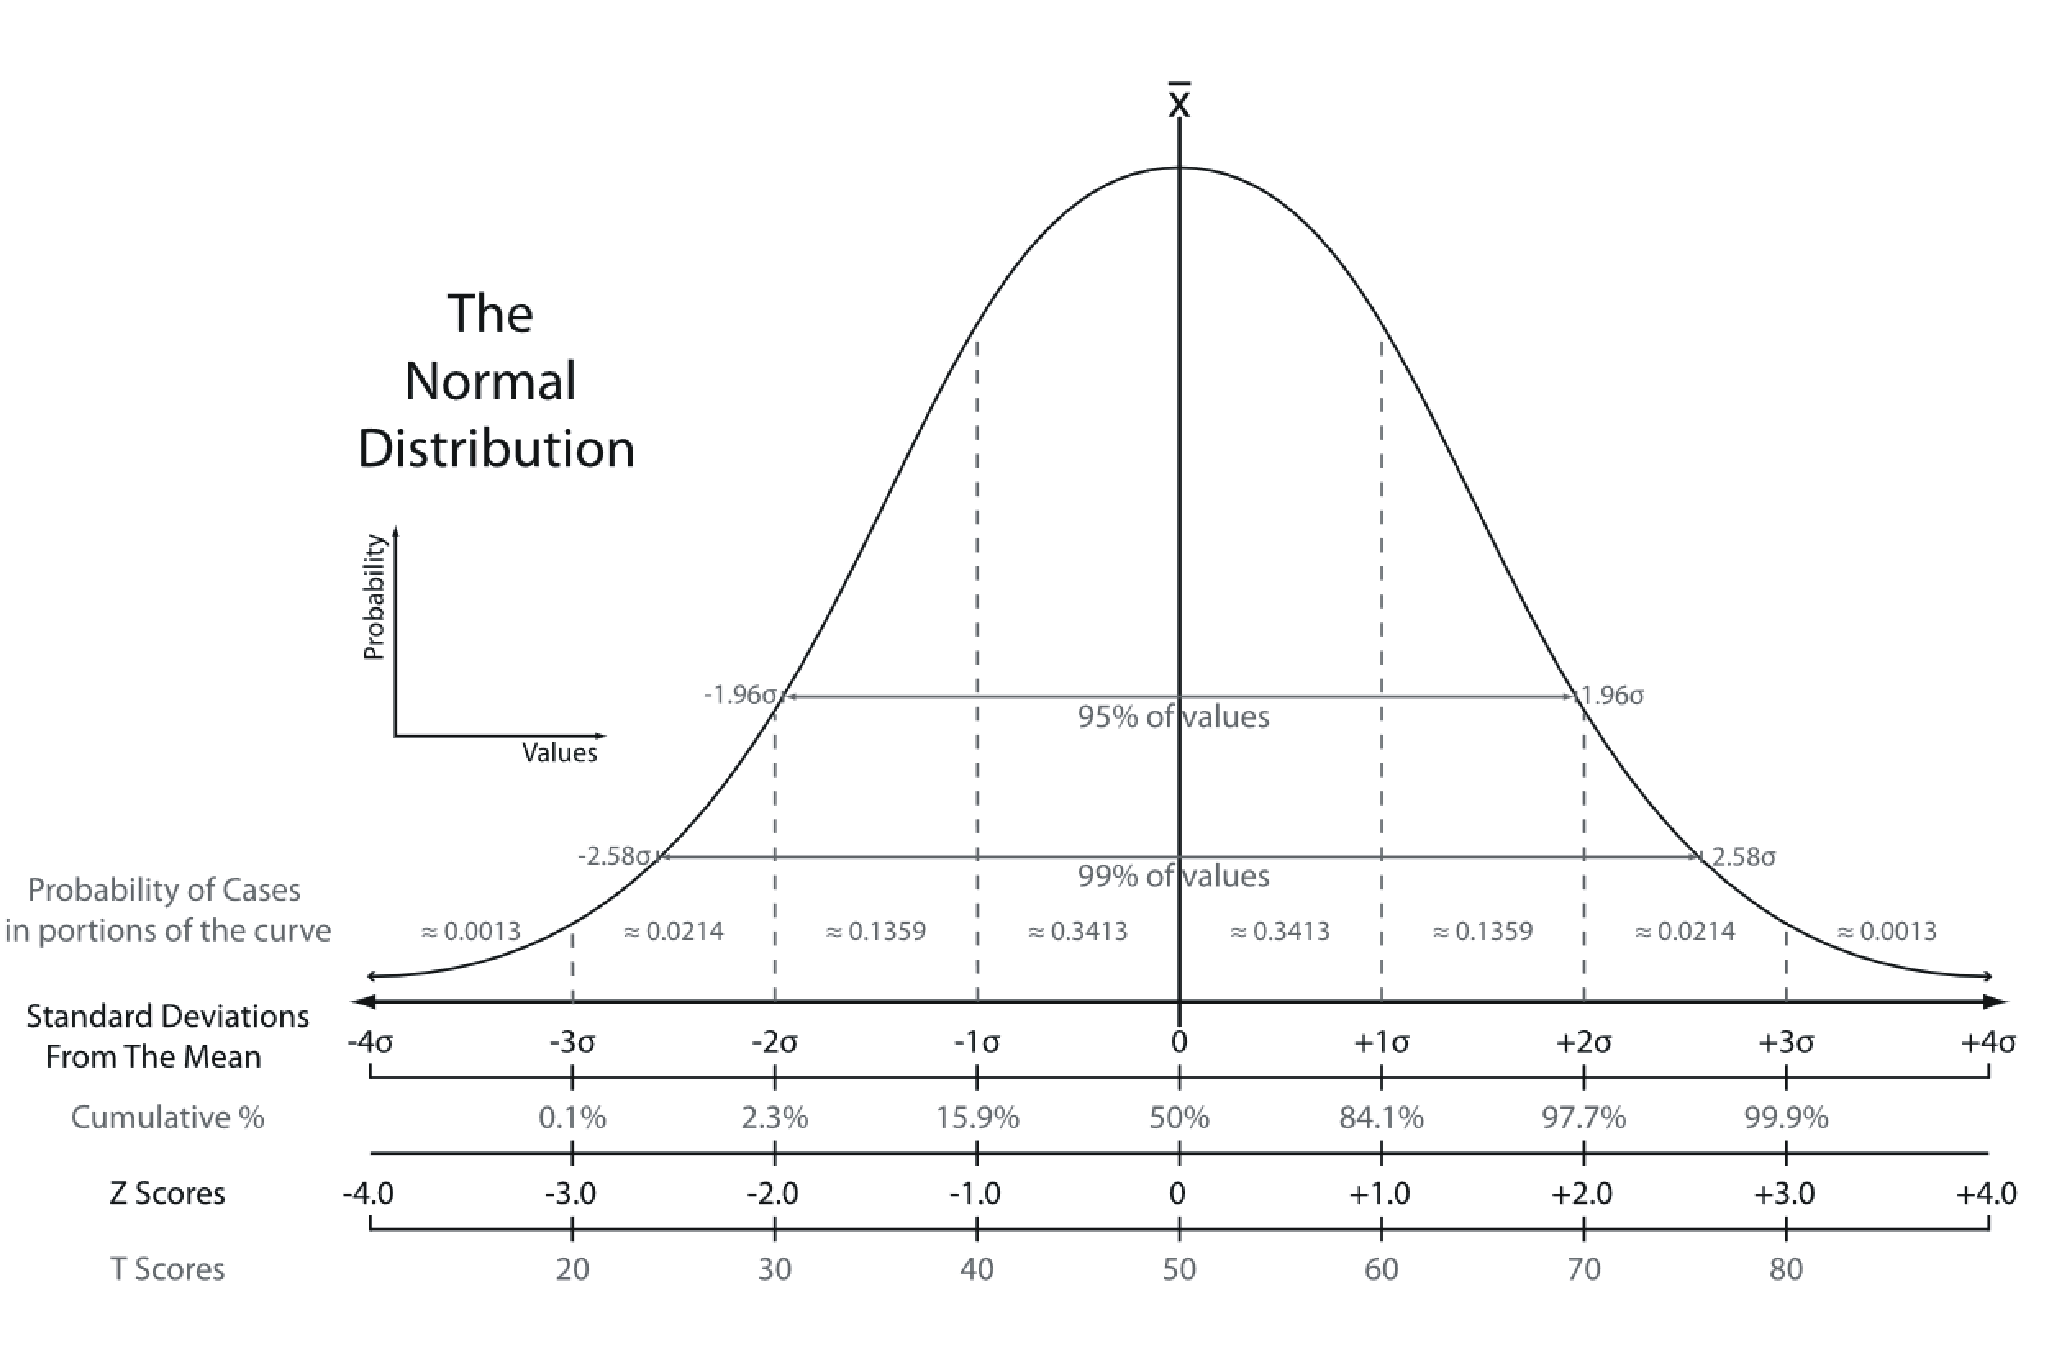
\includegraphics[width=150mm]{06_vorlesung/media/StandardScore.png}
		\caption{Die Standard-Normalverteilung $\mathcal{N}(0,\sigma^2)$ mit den entsprechenden Z-Werten.\newline
		Quelle: https://en.wikipedia.org/wiki/Standard\_score }
		\label{fig:StandardScore}
	\end{center}
\end{figure}
In Abb.\ref*{fig:StandardScore} ist eine Standardnormalverteilung mit den
Z-Scores (Z-Werten) dargestellt.
Z-Scores können nur berechnet werden, wenn die zugrunde liegende Verteilung bekannt ist.
Im Falle von t-Tests haben wir hingegen auch die Möglichkeit auf die aus der Stichproben
geschätzten Parameter für den Erwartungswert und die Varianz zurückzugreifen.
In Abb.\ref*{fig:StandardScore} ist zusätzlich zu der Größe Z-Score ein  weitere
Größe aufgetragen: T-Score. Diese ist direkt proportional zu den Z-Scores nur mit einer
anderen Normierung, derart skaliert, dass ihr Erwartungswert $50$ ist und die
Standardabweichung den Wert $10$ annimmt.

Entsprechend der internationalen Norm \cite{ISO13528} kann der Z-Wert für den Vergleich eines
Messwertes $x_{i}$ eines Labors~$i$ mit dem Referenzwert $x_\mathrm{ref}$, der eine
Standardabweichung (Standardunsicherheit) $\sigma_\mathrm{ref}$ hat, verglichen werden.
Es wird folgender Z-Score berechnet und anschließend bewertet:
\begin{equation}
 z_i = \frac{x_{i}-x_\mathrm{ref}}{\sigma_\mathrm{ref}}
\end{equation}
Nach \cite{ISO13528} gibt es die folgende übliche Interpretation für die Bewertung:
\begin{itemize}
	\item Ein Ergebnis mit $|z_i| \le 2.0$ ist noch akzeptabel.
	\item Ein Ergebnis mit $ 2.0 < |z_i| < 3.0$ gibt ein Warnsignal.
	\item Ein Ergebnis mit $|z_i| \ge 3.0 $ wird als nicht akzeptierbar bewertet.
\end{itemize}
Sind die erweiterten Unsicherheiten sowohl des Referenzlabors $U_\mathrm{ref}$ als auch
des Teilnehmerlabors des $i$-ten Partners $U_{i}$ für das
Überdeckungsintervall $[-2 u; 2 u]$ zum 95,45\% Vertrauensniveau bekannt,
so kann der sogenannte \textbf{En-Wert} berechnet werden.

In der vorigen Vorlesung hatten wir die Prüfgröße
$T = \frac{x_1 - x_2}{\sqrt{\bar s_1^2 + \bar s_2^2}}$, die prüft ob zwei Stichproben mit ihren Erwartungswerten
$x_1$ und $x_2$ zur selben Grundgesamtheit gehören.
Dieser Hypothesentest prüft diese Größe auf $|T| > k$. Der Parameter $k$ steht hier allgemein für das Quantil,
also für $z_{1-\alpha/2}$ im Falle der Verwendung der Standardnormalverteilung wie sie hier in Abb.~\ref{fig:StandardScore}
dargestellt ist. Er steht für das Quantil $t_{1-\alpha/2,\nu}$ im Falle der Verwendung der t-Verteilung ($\alpha$: Signifikanzniveau, $\nu$:
Freiheitsgrad). Ferner steht der Parameter $k$ auch für das Quantil einer Posteriorverteilung, also den Faktor
eines \textsl{Credible} Intervalls, weshalb er allgemein \textsl{Erweiterungsfaktor} genannt wird.

Wenn wir eine Unsicherheit $u_i$ eines Labors vorliegen haben, die beispielsweise $\bar s_i$, d.h. die Standardabweichung  eines Mittelwerts,
sein kann, und haben wir ein symmetrisches Überdeckungsintervall, wie es bei normalverteilten oder t-verteilten Zufallsgrößen
der Fall ist, so ist die halbe Breite des Überdeckungsintervalls $U_i = k u_i$. Dabei wird $U_i$ die \textsl{erweiterte Messunsicherheit} genannt.

Jetzt dividieren wir die Prüfgröße $T$ durch das Quantil bzw. den Erweiterungsfaktor $k$
$$
\frac{T}{k} = \frac{x_1 - x_2}{k \sqrt{\bar s_1^2 + \bar s_2^2}}  = \frac{x_1 - x_2}
{\sqrt{(k \bar s_1)^2 + (k \bar s_2)^2}}
$$
und führen die bei Ringvergleichen allgemein verwendete Bezeichnung $E_n := T /k$ ein,
so dass die Prüfgröße mit $U_i = k u_i$ bzw.\  $U_i = k \bar s_i$ wie folgt aussieht:
\begin{equation}
E_\mathrm{n} = \frac{x_{i}- x_\mathrm{ref}}{\sqrt{U_{i}^2+U_\mathrm{ref}^2}}
\label{eq:EnWert}
\end{equation}
Der \textbf{En-Wert} gibt an, wie gut der Laborwert $x_{i}$ mit dem
Referenzwert $x_\mathrm{ref}$ übereinstimmt. Es werden hier die erweiterten Messunsicherheiten $U$ für $k=2$ kombiniert.
Da hier mit den erweiterten Unsicherheiten gerechnet wird, liegen die Grenzen der akzeptablen Werte nicht bei 2 sondern bei 1.
$|E_n|$ ist gemäß t-Test zu bewerten (siehe auch \cite{ISO13528}):
\begin{itemize}
	\item $|E_\mathrm{n}| \leq 1$: Die Nullhypothese wird angenommen und gilt als Indikator für eine gute Übereinstimmung
	\item $|E_\mathrm{n}| > 1$: Die Nullhypothese wird abgelehnt und gilt als Indikator, dass die Messdaten nicht konsistent zueinander sind.
\end{itemize}

\section{Auswertung von Ringvergleichen ohne Referenzlabor}
\subsection{Vorgehensweise}
Ringvergleiche zwischen den NMIs (\textsl{National Metrology Institutes}), sog.
\textbf{Key-Com\-pari\-sons} dienen u.a. dazu einen Referenzwert (KCRV: \textsl{key comparison reference
value}) mit einer zugeordneten Unsicherheit festzulegen.
Der Grad der Übereinstimmung der Messdaten von teilnehmenden Instituts $i$ zum Referenzwert ist hier gesucht. Es gibt keinen Referenzwert, weil man a priori nicht davon ausgehen kann, dass es ein Staatsinstitut gibt, das signifikant besser messen kann als alle anderen.
Ein mögliches Auswerteverfahren, das häufig Anwendung findet, ist bei
\cite{Cox02} beschrieben. Bei diesem Auswerteverfahren müssen
folgende 3 Voraussetzungen erfüllt sein:
\begin{itemize}
	\item Jeder teilnehmende Partner $i$ ($i=1, \dots, N$) stellt Messdaten $x_i$ mit
	beigeordneter Messunsicherheit $u(x_i)$ eines Prüflings bereit. Der
	Prüfling muss eine gute Stabilität - auch während des Transportes -
	aufweisen.
	\item Jeder Partner stellt Messdaten zur Verfügung, die
	statistisch unabhängig von den anderen Partnern sind. D.h. es darf keine
	Messung eines Partners $i$ von einem anderen Partner $j$ mit $i \ne j$ abhängen.
	\item Die Messdaten jedes Partners (Instituts) sind normalverteilt.
\end{itemize}

Gegeben sind $N$ teilnehmende Institutionen mit $i=1,\dots,N$. Jeder
Partner/Institut $i$ stellt ein Messergebnis der Messgröße zur Verfügung, also einen Schätzwert $x_i$ und eine zugeordnete Standardmessunsicherheit
$u(x_i)$.
Der Ablauf der Auswertung sieht wie folgt aus:
\begin{itemize}
\item \textbf{Schritt 1:}  \newline
Da kein Referenzwert vorliegt, wird in diesem Fall ein gewichteter Mittelwert $\tilde x$ aus den Messergebnissen aller Partner bestimmt. Benutze dazu das inverse der Quadrate der zugeordneten Standardmessunsicherheiten als Gewichte:
\begin{equation}
\tilde x = \frac{x_1/u^2(x_1)+ \cdots + x_N/u^2(x_N)}{1/u^2(x_1)+ \cdots 1/u^2(x_N)} = \frac{\sum\limits_{i=1}^{N} x_i / u^2(x_i)}
{\sum\limits_{i=1}^{N} u^{-2}(x_i)}
\label{eq:referenzgleichepartner}
\end{equation}
\item \textbf{Schritt 2:}  \newline
Bestimme die Standardabweichung des gewichteten Mittelwertes $u(\tilde x)=\sigma(\tilde x)$:
\begin{equation}
\frac{1}{u^2(\tilde x)} = \frac{1}{u^2(x_1)} +\cdots + \frac{1}{u^2(x_N)}
\label{eq:Standardabweichung_Mittelwert}
\end{equation}
\item \textbf{Schritt 3:}  \newline
Führe einen Konsistenzcheck durch, ob die angegeben Messergebnisse
konsistent zueinander sind. Führe dazu den $\chi^2$-Test
durch mit der $\chi^2$-Variablen (Testgröße $T$):
\begin{equation}
T := \chi^2_\mathrm{obs} = \frac{(x_1 - \tilde x)^2}{u^2(x_1)} + \cdots +
\frac{(x_n-\tilde x)^2}{u^2(x_N)}
\label{eq:T_for_consistencecheck}
\end{equation}
Diese Testgröße weist eher einen kleinen Wert auf, wenn alle Partner
recht dicht am Mittelpartner liegen und natürlich umgekehrt.
Vergleiche diese Testgröße mit dem Quantil der $\chi^2 (\nu)$ -Verteilung
mit Freiheitsgrad $\nu = N-1$ ($N$ Anzahl der Partner),
die am Messvergleich teilgenommen haben.
Der Konsistenzcheck \textbf{schlägt fehl}, wenn die folgende Bedingung
erfüllt ist:
\begin{equation}
\mathrm{Pr}\left(\chi^2(\nu) > T\right) < 0.05
\label{eq:consistencecheck}
\end{equation}
\glqq Pr\grqq~steht für \glqq Probability (Wahrscheinlichkeit)\grqq.
Der $\chi^2$-Test verlangt als Voraussetzung, dass die Messergebnisse
normalverteilt sind.

\item \textbf{Schritt 4:}  \newline
Falls der Konsistenzcheck nicht fehlschlägt, wird der Wert $\tilde x$ als
Referenzwert (KCRV: key comparison reference value) $x_\mathrm{ref}$ akzeptiert
mit der Unsicherheit $u(x_\mathrm{ref}) = u(\tilde x)$. Nun kann der \textbf{Grad
der Übereinstimmung} $d_i = x_i - x_\mathrm{ref}$ der Partner $i=1,\dots, N$ mit dem Referenzwert $x_\mathrm{ref}$ wie folgt bestimmt werden.
Wir definieren die normierten Gewichte $\tilde w_i$
\begin{equation}
\tilde w_i := \frac{u^2(x_\mathrm{ref})}{u^2(x_i)}
\label{eq:anteile}
\end{equation}
mit
\begin{equation}
\sum_{i=1}^{N} \tilde w_i = 1 .
\label{eq:normierung}
\end{equation}
Der Referenzwert $x_\mathrm{ref} \equiv \tilde x$ aus Gl.~(\ref{eq:referenzgleichepartner}) ergibt sich wie folgt:
\begin{equation}
x_\mathrm{ref} = \sum_{i=1}^{N} \tilde w_i\; x_i
\label{eq:referenzgleichepartner2}
\end{equation}

Für den Grad der Übereinstimmung erhalten wir:
\begin{equation}
d_i = x_i - x_\mathrm{ref} = x_i - \sum_{j=1}^{N} \tilde w_j x_j
= x_i - \tilde w_i x_i - \sum_{\substack{j=1 \\ j \neq i}}^{N} \tilde w_j x_j
= (1-\tilde w_i)x_i - \sum_{\substack{j=1 \\ j \neq i}}^{N} \tilde w_j x_j
\end{equation}
Wenn die Messungen nicht gegenseitig voneinander abhängen, so kann
zur Berechnung der Unsicherheit von $d_i$ das Gesetz der Fortpflanzung
der Unsicherheiten angewendet werden. (Hinweis: Sind ein Modell mit $y=f(x_1, x_2)$ und
die dazugehören Unsicherheiten $u(x_1)$ sowie $u_(x_2)$ gegeben, so ergibt sich die Unsicherheit von
$y$ bei Nichtkorrelation von $x_1$ und $x_2$ nach dem Gesetz der Fehlerfortpflanzung zu:
$u^2(y)=\left(\frac{\partial f}{\partial x_1}\right)u^2(x_1)+\left(\frac{\partial f}{\partial x_2}\right)u^2(x_2)$)

Für die Unsicherheit der Differenz $d_i$ ergibt sich somit:
\begin{eqnarray}
u^2(d_i) &=& \left( \frac{\partial d_i}{\partial x_i} \right)^2 \cdot u^2(x_i) +  \sum_{\substack{j=1 \\ j \neq i}}^{N}
\left( \frac{\partial d_i}{\partial x_j} \right)^2 \cdot u^2(x_j) \\
&=&  (1-\tilde w_i)^2 u^2(x_i) + \sum_{\substack{j=1 \\ j \neq i}}^{N} \tilde w_j^2 u^2( x_j) \\
&=& ((1-\tilde w_i^2)-\tilde w_i^2)u^2(x_i) + \sum_{j=1}^{N} \tilde w_j^2 u^2(x_j)
\end{eqnarray}
Mit Gl.(\ref{eq:anteile}) ergibt sich:
\begin{equation}
u^2(d_i) = (1-2\tilde w_i^2)u^2(x_i) + \sum_{j=1}^{N} \tilde w_j u^2(x_\mathrm{ref})
\end{equation}
Mit Gl.(\ref{eq:anteile}) und Gl.(\ref{eq:normierung}) ergibt sich daraus:
\begin{eqnarray}
u^2(d_i) &=& u^2(x_i) - 2u^2(x_\mathrm{ref}) + u^2(x_\mathrm{ref}) \sum_{j=1}^{N}\tilde w_j
\nonumber \\
  &=& u^2(x_i) -u^2(x_\mathrm{ref})
\end{eqnarray}
Auch hier kann nun wieder ein En-Wert angeben werden. Da alle Größen normalverteilt sind, sind die erweiterten Unsicherheiten für einen
Erweiterungsfaktor von $k=2$, $U(x_i) = k \cdot u(x_i) =2 \cdot u(x_i)$. Damit lässt sich der En-Wert mit Gl.(\ref{eq:EnWert}) bestimmen, der den
Grad der Übereinstimmung des beteiligten Partners $i$ mit dem Referenzwert
angibt.
\begin{equation}
E_\mathrm{n}(x_i) = \frac{d_i}{2\sqrt{u^2(d_i)}}
\end{equation}
\end{itemize}

Es gelten wieder die Aussagen von Kapitel 1:
\begin{itemize}
	\item $|E_\mathrm{n}| \leq 1$ ist ein Indikator für eine gute Übereinstimmung.
	\item $|E_\mathrm{n}| > 1 $ ist ein Indikator, dass die Messdaten nicht konsistent zueinander sind.
\end{itemize}
\subsection{Beispiel}
\label{Beispielringvergleich1}
% \textbf{Beispiel} \newline
5 Partner messen ein Massestück von ca. 100 g. Die Ergebnisse
der Partner sind wie folgt (alle Angaben sind in g):
\begin{center}
\begin{tabular}{l | c c c c c}
$i$	& 1 & 2 & 3 & 4 & 5 \\	\hline
$x_i / \mathrm{g}$ & 99.82 &  99.05 & 99.17 & 99.20 & 99.38  \\ \hline
$u(x_i) / \mathrm{g}$ & 0.80 & 0.63 & 0.86 & 0.82 & 0.98
\end{tabular}
\end{center}
Als Ergebnis erhalten wir: $x_\mathrm{ref} = 99.29$ und $u_\mathrm{ref} = 0.35$.
Mit der Testgröße $T=0.6239$ ergibt sich die Wahrscheinlichkeit
$\mathrm{Pr}\{\chi^2(\nu) > T\} = 0.9604$. Da die Wahrscheinlichkeit größer als 0.05 ist, schlägt der
Konsistenzcheck nicht fehl,
d.h.\ die Daten der 5 Messpartner sind konsistent.

Für die Abweichungen $d_i$ mit $i=1\ldots 5$ erhalten wir:
$$
[0.5274 \;\; -0.2426 \;\; -0.1226  \;\; -0.0926 \;\;  0.0874].
$$
Für die Unsicherheiten $u_d(i)$  mit $i=1\ldots 5$ erhalten wir:
$$
[0.7172 \;\;   0.5209 \;\;   0.7836  \;\;  0.7395 \;\;   0.9137].
$$
Für die En-Werte erhalten wir:
$$
[ 0.3676 \;\;  -0.2329 \;\;  -0.0783 \;\;  -0.0626 \;\;   0.0478].
$$
Das heisst der Partner 5 ist in bester Übereinstimmung mit dem Referenzwert. \\
Der Octave-/Matlab-Code dazu lautet (Hinweis zu Octave: Evtl. ist die Funktion
\texttt{chi2pdf} in Octave noch nicht vorhanden. Dann zuerst das Paket statistics
installieren, \texttt{pkg install -forge package\_name} mit
\texttt{package\_name = statistics} und evtl. den Pfad hinzufügen): \\
% z.~B. \texttt{addpath('C:\textbackslash Octave\textbackslash
% Octave-4.2.1\textbackslash share\textbackslash octave\textbackslash packages')}
\begin{lstlisting}[style=Matlab]
% addpath('C:\Octave\Octave-4.2.1\share\octave\packages');
% clear all;
x = [99.82, 99.05, 99.17 , 99.20 ,99.38];
u_x = [0.80 0.63, 0.86, 0.82, 0.98];
U_x = 2*u_x;

% Anzahl der Freiheitsgrade
nu = 4;

% Schritt 1:
x_ref = sum(x./(u_x).^2) ./ sum(1./(u_x).^2)

% Schritt 2:
u_ref = sqrt(1./sum(1./(u_x).^2))

% Schritt 3:
T = sum((x-x_ref).^2./(u_x.^2))

% Bestimme die Wahrscheinlichkeit Pr der Chi^2-Verteilung fuer Chi^2(\nu) > T:
Pr = 1 - chi2cdf(T,nu)

% Schritt 4: Grad der Uebereinstimmung
d = x-x_ref;
u_d = sqrt(u_x.^2 - u_ref.^2)
En = d./(2*sqrt(u_d.^2))
\end{lstlisting}

\subsection{Identifikation von Ausreißern und Konsistenzcheck}
Wir wollen uns hier noch etwas genauer anschauen, wie man feststellt,
ob die Messdaten eines Ringvergleiches konsistent sind und wie man mit Inkonsistenten umgeht.
Als \textbf{Ausreißer} werden häufig Messwerte deklariert, deren Abweichungen größer
als 3 mal die erweiterte Messunsicherheit des Referenzwertes \cite{GuideKey} sind.
Diese Ausreißer werden in Abstimmung mit dem Partner gelöscht.
Anschließend werden die verbliebenen Daten auf statistische Konsistenz
überprüft. Wir haben dazu bereits in Gl.(\ref{eq:T_for_consistencecheck}) und Gl.(\ref{eq:consistencecheck})
eine Formel angegeben, mit der überprüft werden kann, ob die angegebenen
Messergebnisse (Messwerte mit Unsicherheiten) konsistent zu dem Referenzwert und
dessen Unsicherheit ist. Die Testgröße $T$ basiert auf dem Birge-Test,
welche ebenso ein Test auf die Konsistenz der Messdaten in einem Ringvergleich
ist. Der Birge-Test ist wie der $\chi^2$-Test nur unter folgenden Bedingungen
gültig:
\begin{itemize}
	\item Die gemessenen Messwerte $x_i$ der $N$ Institute sind unkorreliert
	\item Man benötigt Kenntnis über die Verteilungsdichtefunktionen. Es
	wird vorausgesetzt, dass die Größen normalverteilt mit den Unsicherheiten $u(x_i)$ bzw. den Varianzen $\sigma_i$ sind.
\end{itemize}
Das Birge-Verhältnis ist -bis auf die Anzahl der Freiheitsgrade- die Prüfgröße des Chi2-Tests (siehe vorherige Vorlesung)
% Gl.~\ref{chi2testgroesse}).
Es wird folgendes geprüft ($H_0$: Nullhypothese, $H_a$: Alternativhypothese):
\begin{center}
	\begin{tabular}{l | p{14cm} }
	$H_0$	& $u_\mathrm{partner}^2 =  u_\mathrm{ref}^2$:\newline
	Die Stichprobe gehört zu
		einer Grundgesamtheit  mit Varianz $u_\mathrm{ref}^2$\\	\hline
 $H_\mathrm{a}$	& $u_\mathrm{partner}^2 \neq  u_\mathrm{ref}^2$: \newline
 Die Stichprobe gehört nicht zu einer Grundgesamtheit mit Varianz $u_\mathrm{ref}^2$\\
	\end{tabular}
\end{center}

Das \textbf{Birge-Verhältnis} ist definiert als das Verhältnis der Streuungen der Unsicherheiten aller Partner
(bezeichnen wir mit $u_\mathrm{partner}$) zu der Unsicherheit des Referenzwertes $u_\mathrm{ref}$. Es wird
analog der Testgröße des $\chi^2$-Tests, $T = \nu \left(\frac{s}{\sigma_0}\right)^2$ Gl.~\ref{chi2testgroesse}, wie
folgt definiert:
\begin{equation}
R_\mathrm{B} := \frac{u_\mathrm{partner}}{u_\mathrm{ref}}
\quad \text{mit} \quad
\frac{u^2_\mathrm{partner}}{u^2_\mathrm{ref}} \, \propto \,
\nu \left(\frac{s}{\sigma_0}\right)^2.
\end{equation}
Die Varianz aller $N$ Partner ist wie folgt definiert:
\begin{equation}
u^2_\mathrm{partner} := \frac{\frac{1}{N-1} \sum\limits_{i=1}^{N} w_i \left(x_i-x_\mathrm{ref} \right)^2}
{\sum\limits_{i=1}^{N} w_i} \quad \text{mit} \quad w_i = \frac{1}{u^2(x_i)} .
\end{equation}
Entsprechend Gl.(\ref{eq:Standardabweichung_Mittelwert}) ist die Unsicherheit des Referenzwertes wie folgt gegeben
\begin{equation}
u_\mathrm{ref} = \left(\frac{1}{u^2(x_1)} +  \cdots + \frac{1}{u^2(x_N)} \right)^{-\frac{1}{2}},
\end{equation}
so dass für das Birge-Verhältnis gilt
\begin{equation}
R_\mathrm{B} = \sqrt{\frac{1}{N-1} \; \sum_{i=1}^N \left( \frac{x_i-x_\mathrm{ref}}{u(x_i)} \right)^2 }.
		\label{eq:Birge-Verhaeltnis}
\end{equation}

Vergleicht man das Birge-Verhältnis mit der Testgröße $T = \nu \left(\frac{s}{\sigma_0}\right)^2$ in Gl.(\ref{eq:T_for_consistencecheck}) so ergibt sich der Zusammenhang:
\begin{equation}
R_\mathrm{B}^2 = \frac{1}{N-1} \; T
\end{equation}
Bei dem Konsistenzcheck mit dem Birge-Verhältnis wird untersucht, ob
\begin{itemize}
	\item $R_\mathrm{B} \le 1$: Konsistenzcheck ok.
	\item $R_\mathrm{B} > 1$: Konsistenzcheck schlägt fehl.
\end{itemize}
Wenn $R_\mathrm{B} > 1$ ist, bedeutet dies, dass entsprechend Gl.(\ref{eq:Birge-Verhaeltnis}) die Unsicherheiten der Partner
$u(x_i)$ nicht zu der Unsicherheit des Referenzwertes $u(x_\mathrm{ref})$ passen.
Die gemessenen Daten $x_i$ der Partner sind inkonsistent.
Für unser Beispiel Abschnitt \ref{Beispielringvergleich1} erhalten wir $R_\mathrm{B} = 0.39494$.
Damit schlägt der Birge-Test nicht fehl und die Daten sind
danach konsistent. Für die Auswertung eines Ringvergleichs ist es empfehlenswert sowohl das Birge-Verhältnis als auch den $\chi^2$-Test
(siehe Gl.(\ref{eq:consistencecheck})) durchzuführen und zu prüfen, ob beide Tests ok sind.

Häufig wird das Birge-Verhältnis in Gl.(\ref{eq:Birge-Verhaeltnis})
umgeschrieben und in folgender Form dargestellt:
\begin{equation}
R_\mathrm{B}^2 = \sum_{i=1}^N \frac{w_i (x_i - x_\mathrm{ref})^2}{N-1}
\end{equation}
mit den Gewichten $w_i = 1/\sigma_i^2$ für $i=1,2,\ldots, N$ und dem
Referenzwert (gewichteten Mittelwert) $x_{ref}=\sum_i w_i x_i / \sum_i w_i$.
Der Birge Test kann auch bei korrelierten Messdaten $x_1,\ldots ,x_N$, wenn die
Kovarianzen $\sigma_{12},\ldots, \sigma_{(N-1)N}$ gegeben sind, durchgeführt werden, siehe \cite{Kac08}.

\subsection{Paule-Mandel Methode zur Anpassung von Gewichtsfaktoren}

Bei Ringvergleichen kommt es auch mal vor, dass die Messmethoden nicht immer genau die gleichen sind und der Einfluss der verschiedenen Methoden des Vergleichs unterschätzt wird. Wenn sich herausstellt, dass sich Gruppen von Ergebnissen ausbilden, so kann eine Zwischengruppenvarianz ermittelt werden. Dies kann beispielsweise mit der Paule-Mandel Methode erfolgen.

Es kann bei Ringvergleichen vorkommen, dass jeder am Vergleich beteiligte Partner eine
Unsicherheit $U$ angibt, die kleiner ist als der Abstand des Messwertes zu anderen Partnern,
so dass sich ein En-Wert bzw.\ des Birge-Verhältnisses unter Verwendung der Gewichte gemäß Gl.~(\ref{eq:anteile}) größer als Eins ergibt. Durch eine Anpassung der Gewichtsfaktoren durch Hinzufügen einer
zusätzlichen Komponente, die sich aus der Streuung der Ergebnisse von Partner zu Partner ergibt, kann eine bessere Konsistenz erzielt werden.

Der Leitfaden zum Erstellen eines \textsl{Key Comparison Reports}
\cite{GuideKey} empfiehlt als Anpassungsverfahren die \textbf{Paule-Mandel Methode},
bei der die Varianzen durch Additions einer Streuung zwischen Laboratorien
erhöht werden. Dadurch werden die Gewichtsfaktoren $w_i$ verkleinert und damit Referenzwert
$x_\mathrm{ref}$ so angepasst, so dass das Birge-Verhältnis kleiner als Eins werden kann.
Ein Beispiel dazu ist im Anhang B der Richtlinie für Ringvergleiche \cite{GuideKey} zu finden.

Im Folgenden schauen wir uns das Prinzip von Mandel und Paule an, das
in der Publikation \cite{Pau82} zu finden. Es werden zwei eher künstliche Beispiele gewählt, um das Prinzip besser zu verstehen.
In Beispiel I wird eine Messgröße mit zwei verschiedenen Methoden (bzw.\ von zwei verschiedenen Partnern) A und B gemessen.
Die gemessenen Einzelwerte von jedem der beiden Partner sind in Tab. \ref*{tab:Beispiel_I}
angegeben.
\begin{table}[!htb]
	\caption{Messdaten des Beispiels I}
	\begin{center}
	\begin{tabular}{l| rrr |rrr}
		\hline
		Methode/Partner & \multicolumn{3}{c}{A} \vline & \multicolumn{3}{c}{B} \\ \hline
		Gemessener Wert $x_i$ & 1.1 & 1.9 & 1.5 & 16 & 25 & 3 \\ \hline
	\end{tabular}
\end{center}
\label{tab:Beispiel_I}
\end{table}

Der gleichgewichtete Mittelwert $\bar x_I$ über alle Werte beider Partner ist:
 \begin{equation}
 \bar x_I = \frac{1}{N} \sum_{i=1}^N x_i \, = \frac{1}{6}\left( 1.1 + 1.9 + 1.5 + 16 + 25 + 3 \right) \, \approx \, 8.1
 \end{equation}
 Intuitiv würden wir jedoch sagen, dass wir den Messdaten mit der Methode A
 mehr vertrauen schenken würden, als den Messdaten mit der Methode B, da die
 Messdaten der Methode A weniger streuen als die Messdaten mit der Methode B.

 Als zweites Beispiel betrachten wir, dass die Methoden (bzw. Partner) A und B ähnlich
 genau messen, jedoch werden von Partner A einen größeren Stichprobenumfang
 als von Partner B:


 \begin{table}[!htb]
 	\caption{Messdaten des Beispiels II}
 	\begin{center}
 		\begin{tabular}{l| rrrrrr |rr}
 			\hline
 			Methode/Partner & \multicolumn{6}{c}{A} \vline & \multicolumn{2}{c}{B} \\ \hline
 			Gemessener Wert $x_i$ & 2.0 & 1.0 & 1.5 & 1.8 & 1.2 & 1.7
 			& 16.3 & 16.8\\ \hline
 		\end{tabular}
 	\end{center}
 	\label{tab:Beispiel_II}
 \end{table}
Für den gleichgewichteten Mittelwert über alle Werte erhalten wir:
 \begin{equation}
 \bar x_{II} = \frac{1}{N} \sum_{i=1}^N x_i \, = \frac{1}{8}\left( 2.0 + 1.0 + 1.5 + 1.8 + 1.2 + 1.7 + 16.3 + 16.8 \right) \, = \, 5.2875
\label{eq:einfachesMittelII}
 \end{equation}
Es fällt auf, dass die beiden Werte von Partner B zueinander passen, sich aber deutlich von denen von Partner A unterscheiden.

Die beiden Mittelwerte der jeweiligen Partner A und B sind
 \begin{equation}
 \bar x_{II,A} = \frac{1}{6}\left( 2.0 + 1.0 + 1.5 + 1.8 + 1.2 + 1.7 \right) = 1.533,
\quad \bar x_{II,B} = \frac{1}{2}\left( 16.3 + 16.8 \right) = 16.550
 \label{eq:Mittelwerte_x_II_A_B}
 \end{equation}

\begin{comment}

\textcolor{red}{\textbf{Dieses würde ich hier an dieser Stelle gar nicht bringen, auch wenn es in Pau82
so präsentiert wird, weil Du ja hier in diesem Skript schon mit den Gewichten als Kehrwert
der Varianzen für den Referenzwert, der aus dem gewichteten Mittel der Resultate aller Partner
gewonnen wurde, um En-Werte für gleiche Partner zu bestimmen.}}


\textcolor{red}{zunächst hatte ich entlang am Pau82 die Sachen so nachgerechnet und verstanden, wie
Paule und Mandel sie argumentiert hatte, dann wurde mir langsam klar, dass wir in unseren Vorlesungen
aber längst an dem Punkt angekommen sind, dass man die Kehrwerte der Varianzen nimmt und nicht
anfängt die Mittelwerte einfach zu mitteln $\Rightarrow$ alles Blaue hiernach hier wegnehmen}

\textcolor{blue}{und der Mittelwert dieser beiden Mittelwerte ist
 \begin{equation}
  \bar x_{II,AB} = \frac{1}{2}\left( 1.533 + 16.550 \right) = 9.0417
 \label{eq:Mittelwerte_x_IIAB}
 \end{equation}
 Dadurch dass wir Mittelwerte mitteln erhalten wir eine andere Wichtung: $\frac{\sum w_i x_i}{\sum w_i}$:
$$
\frac{1}{2} \left( \frac{1}{6} \left(\sum\limits_{i=1}^6 x_i \right) \; + \;
    \frac{1}{2} \left(\sum\limits_{i=7}^8 x_i \right)  \right) =
 \frac{1}{12} \left(\sum\limits_{i=1}^6 x_i \right) \; + \;
    \frac{1}{4} \left(\sum\limits_{i=7}^8 x_i \right)
$$
also
$$
\frac{w_i}{\sum\limits_{i=1}^8 w_i} \, = \,
\left\{ \begin{array}{ccl}
\frac{1}{12} & \text{f{\"u}r} & i = 1,\dots,6 \\
\frac{1}{4} & \text{f{\"u}r} & i = 7, 8
\end{array} \right.
$$
Diese Art der Wichtung, die Einzelwerte zu gewichten, führt dazu dass Stichprobe B
sehr viel stärker gewichtet wird, in diesem Beispiel um einen Faktor $3$ mit $\frac{1}{4} = \frac{3}{12}$.
Es macht jedoch mehr Sinn, die Gewichte danach zu richten, wie genau die Größen sind,
im Sinne von der Frage wie breit oder schmal die Wahrscheinlichkeitsdichteverteilung ist.}
\end{comment}

Wir haben im Laufe dieser Vorlesungsreihe bereits gesehen, dass
Messergebnisse mit größerer Unsicherheit sinnvollerweise mit geringerer
Wichtung zu berücksichtigen sind, so dass Gewichte
deshalb aus dem Kehrwert der Varianzen bestimmt werden. Der Grund dafür liegt darin,
dass die Varianz des gewichteten Mittelwertes $x_\mathrm{ref}$ minimiert wird,
wenn die Gewichte als Reziprokwert der Varianzen der Einzelwerte berechnet werden.
In Gl.~(\ref{eq:referenzgleichepartner2})
haben wir deshalb zur Ermittlung des Referenzwertes $x_\mathrm{ref}$ beim
Ringvergleich mit gleichwertigen Partnern gerechnet mit
\begin{equation*}
    w_i = \frac{1}{u^2_i}
\end{equation*}
und
\begin{equation*}
 x_\mathrm{ref} = \frac{\sum\limits_{i=1}^N w_i x_i}{\sum\limits_{i=1}^N w_i} .
\end{equation*}

\begin{comment}
\textcolor{red}{wahrscheinlich macht es keinen Sinn mit der empirischen Varianz
anzufangen, sondern direkt mit der empirischen Var des Mittelwertes, also nehme ich
diesen Teil wieder zurück}
\textcolor{blue}{Verwenden wir für die Unsicherheit $u_i$ die empirische Varianz
$u_i = \operatorname{Var}(x_i)$ für Beispiel II folgende Werte
$$
\operatorname{Var}(x_{II,A}) =
\frac{1}{6-1} \sum\limits_{k=1}^{6} \left(x_{II,k} - \bar x_{II,A} \right)^2 = 0.14267
$$
und
$$
\operatorname{Var}(x_{II,B}) = \frac{1}{2-1} \sum\limits_{k=7}^{8} \left(x_{II,k} - \bar x_{II,B} \right)^2
= 0.12500
$$
so erhalten wir für die beiden Gewichte $w_A = 7.0093$ und $w_B = 8.0000$, die beide fast gleich.
Der gewichtete Mittelwert, der als Referenzwert für En-Tests und das Birge-Verhältnis genutzt wird ist damit
$$
x_\mathrm{ref} \; = \; \frac{7.0093 \cdot 1.533 \; + \; 8.0000 \cdot 16.550}{7.0093 + 8.0000}
\; = \; 9.5372
$$
Nach Gl.~(\ref{eq:Birge-Verhaeltnis}) das Birge-Verhältnis hierfür
$$
R^2_\mathrm{B} \; = \; \frac{1}{N-1} \; \sum_{i=1}^N \left( \frac{x_i-x_\mathrm{ref}}{u^2(x_i)} \right)^2 \; = \;
 \frac{1}{2-1} \, \left( \frac{\left(1.5333 - 9.5372\right)^2}{0.14267}
 \, + \, \frac{ \left( 16.550 - 9.5372 \right)^2}{0.12500} \right) = 842.47 \gg 1
$$
--nix!}
\end{comment}

Wenn die Varianzen
der Methode A und B ähnlich sind, so kann eine gemeinsame (gepoolte) Varianz der beiden Methoden berechnet werden (siehe 5. Vorlesung):
\begin{equation}
\operatorname{Var}(x_{ref}) = \frac{\sum\limits_{i=1}^6 \left(x_{A,i}-\bar x_A\right )^2+\sum\limits_{i=1}^2 \left(x_{B,i}-\bar x_B\right )^2}{(6-1)+(2-1)} = 0.1397
\end{equation}

Da es sich um den Vergleich der Mittelwerte der beiden Stichproben A und B handelt, verwenden wir
für die Unsicherheit $u_i$ die Varianz des Mittelwertes, also
$u_i = \operatorname{Var}(\bar x_i)$. Sie ist definiert als
$$
\operatorname{Var}(\bar x_i) = \frac{\operatorname{Var}(x_i)}{N_i}
$$
mit $N_i$ den Anzahl der Wiederholungen für den Mittelwert $\bar x_i$.

Für Beispiel II erhalten wir dann folgende Werte:
$$
\operatorname{Var}(\bar x_{II,A}) = \frac{1}{6(6-1)} \sum\limits_{k=1}^{6} \left(x_{II,k} - \bar x_{II,A} \right)^2 = 0.023778
\quad \text{d.h.} \quad \bar s_A = \sqrt{\operatorname{Var}(\bar x_{II,A})} = 0.154
$$
und
$$
\operatorname{Var}(\bar x_{II,B}) = \frac{1}{2(2-1)} \sum\limits_{k=7}^{8} \left(x_{II,k} - \bar x_{II,B} \right)^2 = 0.062500
\quad \text{d.h.} \quad \bar s_B = \sqrt{\operatorname{Var}(\bar x_{II,B})} = 0.250
$$
so erhalten wir für die beiden Gewichte $w_A = 42.056$ und $w_B = 16.000$.
Der gewichtete Mittelwert, der als Referenzwert für En-Tests und das Birge-Verhältnis genutzt wird, ist damit
$$
x_\mathrm{ref} \; = \; \frac{42.056 \cdot 1.533 \; + \; 16.000 \cdot 16.550}{42.056 + 16.000}
\; = \; 5.6716
$$
Nach Gl.~(\ref{eq:Birge-Verhaeltnis}) das Birge-Verhältnis hierfür
$$
R^2_\mathrm{B} \; = \; \frac{1}{N-1} \; \sum_{i=1}^N \left( \frac{x_i-x_\mathrm{ref}}{u(x_i)} \right)^2 \; = \;
 \frac{1}{2-1} \, \left( \frac{\left(1.5333 - 5.6716\right)^2}{0.023778}
 \, + \, \frac{ \left( 16.550 - 5.6716 \right)^2}{0.0625} \right) = 2613.7
$$
also
$$
R_\mathrm{B} \; = \; \sqrt{2613.7} \, = \, 51.1  \gg 1
$$

% https://iopscience.iop.org/article/10.1088/0026-1394/51/5/516/meta

Wir sehen, dass die Varianzen der Mittelwerte der beiden Partner A und B im Verhältnis zur
Differenz zwischen den beiden Partnern sehr klein ist, oder umgekehrt gesagt liegen die
Mittelwerte der Methoden A und B sehr weit auseinander im Verhältnis zu den Varianzen.
Die Varianzen $\operatorname{Var}(\bar x_A)$ und $\operatorname{Var}(\bar x_A)$ beschreiben
nur die interne Streuung, also nur die Streuung der jeweiligen Stichproben A und B.
Die Wahrscheinlichkeitsverteilungen werden durch die beiden Parameter Erwartungswert,
also hier Mittelwert und Varianz charakterisiert und wir hatten bei den Hypothesentests
gelernt, auf beides zu prüfen. Wir haben gesehen, dass Stichproben einer gemeinsamen
Grundgesamtheit angehören, wenn beides, Mittelwert und Varianz zueinander passen.

Bei den Ringvergleichen, bei denen von verschiedenen Laboratorien oder Instituten mit
unterschiedlichen Methoden oder jedenfalls unabhängigen experimentellen Aufbauten die
Ergebnisse verglichen werden, kann beobachtet werden, dass entweder die
Schätzer (empirischen Erwartungswerte) oder die empirischen Varianzen oder sogar
beides nicht zusammen passen. In der Praxis kommt es vor, dass die jeweiligen
Labore oder Institute ihre Methode immer weiter optimiert haben und ihre Genauigkeit
erhöht haben, dass jedoch verbleibende, unerkannte systematische Effekte vorhanden sind.
Dass es Unterschiede gibt, tritt erst bei dem Vergleich zutage und es lässt sich
im Rahmen der gesetzten Zeit für das Projekt des Vergleichens nicht aufklären.
In solchen Fällen lebt man dann damit, dass es auch zwischen den unterschiedlichen
Methoden bzw.\ Laboren eine Streuung gibt.

Statistisch wird dies damit ausgedrückt, dass die Stichproben auf den verschiedenen
Laboren zu verschiedenen Grundgesamtheiten gehören.
Konkret bedeutet das, dass für die Gewichte zusätzlich zur Varianz des Mittelwert
zur jeweiligen Methode/ des jeweiligen Laboratoriums
(Streuung innerhalb einer Gruppe, \textsl{within group variability})
auch eine Varianz der Methoden/Laboratorien (Streuung zwischen Gruppen,
\textsl{between group variability}) eingeführt.
Die Streuung zwischen den Gruppen, die Varianz $s^2_\mathrm{b}$ wird
iterativ geschätzt. Für die verschiedenen Partner oder Stichproben $A$ und $B$
verwenden wir jetzt die Notation $S_i$, hier also $S_1 = A$ und $S_2 = B$, um
die Gleichungen allgemein aufschreiben zu können.
\begin{equation*}
\operatorname{Var}(\bar x_{S_i,\mathrm{c}}) \; = \;
\operatorname{Var}(\bar x_{S_i}) \; + \; s^2_\mathrm{b} \; = \;
\frac{1}{M_i (M_i - 1)} \sum\limits_{k \in S_i}
\left( x_{k} - \bar x_{S_i} \right)^2
\; + \; s^2_\mathrm{b}
\end{equation*}
mit $M_i$ für den Stichprobenumfang zu $S_i$ -
oder kürzer aufgeschrieben mit $i$ als Index für die Nummerierung der Partner
und für die Varianzen der Mittelwerte bzw.\ Messergebnisse
der Partner
$u^2_i = \bar s^2_i = \operatorname{Var}(\bar x_{S_i})$
bzw.\ für die Konsensusvarianzen
$\bar s^2_{i,\mathrm{c}} = \operatorname{Var}(\bar x_{S_i,\mathrm{c}})$
\begin{equation}
\bar s^2_{i,\mathrm{c}} \; = \; \bar s^2_i \; + \; s^2_\mathrm{b}
\quad i=1,2
\label{eq:consensusVariability}
\end{equation}
wobei der Index b für \textsl{between} und c für \textsl{consensus}
stehen. Auch die Mittelwerte bzw.\ allgemein die Messergebnisse der
jeweiligen Partner schreiben wir jetzt in der Form $\bar x_{S_i} = \bar x_i$.

Die Gewichte für den \textsl{Consensus Value}, dem besser übereinstimmenden
Wert für die Messgröße, sind damit dann
\begin{equation*}
w_{i,\mathrm{c}} \, = \; \frac{1}{\operatorname{Var}(\bar x_{S_i,\mathrm{c}})} \; = \;
\left(\frac{1}{M_i (M_i - 1)} \sum\limits_{k \in S_i}
\left( x_{k} - \bar x_{S_i} \right)^2
\; + \; s^2_\mathrm{b} \right)^{-1}
\end{equation*}
mit $M_i$ für den Stichprobenumfang zu $S_i$
und dasselbe in der kürzeren Notation geschrieben
\begin{equation}
w_{i,\mathrm{c}} \, = \, \frac{1}{\bar s^2_{i,\mathrm{c}}} \, = \, \frac{1}{\bar s^2_j \; + \; s^2_\mathrm{b}} .
\label{eq:consensusWeights}
\end{equation}
Der Konsenzreferenzwert aus den Werten aller $N$ Partner ist dann
\begin{equation}
x_\mathrm{ref, c} \, = \,
\frac{\sum\limits_{i=1}^N w_{i,\mathrm{c}} x_i}{\sum\limits_{i=1}^N w_{i,\mathrm{c}} }.
\label{eq:consensusMean}
\end{equation}
Das Birge-Verhältnis für diese Konsensuswerte ist somit
\begin{equation}
R_\mathrm{B} \; = \; \sqrt{ \frac{1}{N-1} \, \sum\limits_{i=1}^N
\frac{1}{\bar s^2_i \; + \; s^2_\mathrm{b}} \, \left(\bar x_i - x_\mathrm{ref, c}\right)^2}.
\end{equation}

\textbf{Schätzen der Zwischengruppenvarianz $s^2_\mathrm{b}$}
\begin{quote}
Geschätzt wird die Zwischengruppenvarianz $s^2_\mathrm{b}$ gemäß Paule und Mandel \cite{Pau82} als
diejenige Varianz, für die die Ergebnisse der Partner konsistent sein sollen, also für die
das Birge-Verhältnis gegen Eins streben soll: $R_\mathrm{B} \rightarrow 1$.
\end{quote}
Die Optimierungsaufgabe formulieren wir für das Quadrat des Birge-Verhältnisses,
um eine Kostenfunktion zu haben, die sich einfacher linearisieren lässt. Dies
geht ganz gut, weil $1^2 = 1$ ist, also $R^2_\mathrm{B} \rightarrow 1$, d.h.
\begin{equation*}
\frac{1}{N-1} \, \sum\limits_{i=1}^N
\frac{1}{\bar s^2_i \; + \; s^2_\mathrm{b}} \, \left(\bar x_i - x_\mathrm{ref, c}\right)^2 \rightarrow 1
\end{equation*}
oder genauer ausgedrückt
\begin{equation}
\min_{s^2_\mathrm{b}} \left\{\frac{1}{N-1} \, \left( \sum\limits_{i=1}^N
\frac{1}{\bar s^2_i \; + \; s^2_\mathrm{b}} \, \left(\bar x_i - x_\mathrm{ref, c}\right)^2  \right) \, - \, 1\right\}.
\label{eq:x_bet_Bedingung}
\end{equation}

Diese Optimierungsaufgabe hat eine Kostenfunktion
$Q(s^2_\mathrm{b}) = \frac{1}{N-1} \, \left( \sum\limits_{i=1}^N
\frac{1}{\bar s^2_i \; + \; s^2_\mathrm{b}} \, \left(\bar x_i - x_\mathrm{ref, c}\right)^2  \right) \, - \, 1$
die von dem zu schätzenden Parameter, der Zwischengruppenvarianz
$v := s^2_\mathrm{b}$ nicht-linear abhängt, so dass sie iterativ zu lösen ist, es handelt sich also
nichtlineare Optimierung wie wir es in Kapitel~\ref{nonlinOpti} besprochen haben.

Wir entwickeln die Kostenfunktion in
eine Taylorreihe bis zum linearen Term
\begin{equation}
Q(v_0 + \operatorname{d} v_0) \approx
Q_0 + \left.\left( \frac{\partial Q}{\partial v}\right)
\right|_{v=v_0} \operatorname{d} v_0
\end{equation}
Mit $Q(v) \rightarrow 0$ setzen wir für den ersten
Iterationsschritt
\begin{equation}
Q_0 + \left.\left( \frac{\partial Q}{\partial v}\right)
\right|_{v=v_0} \operatorname{d} v_0 = 0
\end{equation}
und lösen dies nach $\operatorname{d} v_0$ auf zu
\begin{equation}
\operatorname{d} v_0 = -\left. \left( \frac{Q_0}{\frac{\partial Q}{\partial v}}\right) \right| _{v=v_0}
\end{equation}
Wir beginnen mit dem Startwert für $v_0$, indem wir ihn auf $v_0 = 0$ setzten, so dass wir
mit dem sehr großen Birge-Verhältnis beginnen und iterativ die Zwischengruppenvarianz
erhöhen, um das Birge-Verhältnis solange zu reduzieren bis es Eins wird.
Im nächsten Schritt setzen wir $v_1 = v_0 + \operatorname{d} v_0$.
Dies setzten wir fort mit
\begin{equation}
v_{k+1} =v_k + \operatorname{d} v_k
\end{equation}
bis $Q$ zu einem Minimum möglichst nahe bei Null konvergiert.

Die Ableitung der Kostenfunktion $Q$ nach der Zwischengruppenvarianz ist
\begin{equation*}
\frac{\partial Q}{\partial v} = \frac{1}{N-1} \, \left( \sum\limits_{i=1}^N
\frac{\partial }{\partial v} \frac{1}{\bar s^2_i \; + \; v} \, \left(\bar x_i - x_\mathrm{ref, c}\right)^2  \right) \, - \, 0
\end{equation*}
d.h.
\begin{equation*}
\frac{\partial Q}{\partial v} = \frac{1}{N-1} \, \sum\limits_{j=1}^N  \left(\bar x_j - x_\mathrm{ref, c}\right)^2
\frac{\partial }{\partial v} \frac{1}{\bar s^2_i \; + \; v}
\end{equation*}
d.h.
\begin{equation}
\frac{\partial Q}{\partial v} = \frac{1}{N-1} \, \sum\limits_{i=1}^N  \left(\bar x_i - x_\mathrm{ref, c}\right)^2
\frac{-1}{\left(\bar s^2_i \; + \; v\right)^2}
\end{equation}
Die Iterationen laufen, solange $R_\mathrm{B}$ größer als Eins ist und eine maximale Anzahl Iterationsschritte einen Wert von $50$ nicht überschreitet.
In dem hier behandelten Beispiel werden $17$ Iterationsschritte gebraucht, bis die
Optimierung konvergiert und folgendes Ergebnis für die Zwischengruppenvarianz $v = s^2_\mathrm{b}$ liefert.

$$
v = 112.707 \quad \text{d.h.} \quad s_\mathrm{b} = 10.6
$$

\begin{comment}
\textcolor{red}{ich werde hier noch einen Plot erzeugen, der die Gaußverteilungen der
beiden Einzelstichproben zeigt (vielleicht außerdem noch die t-Verteilungen) sowie die
Gaußverteilung ${\cal N}(x_\mathrm{ref} = 9.040, s_\mathrm{b} = 10.6)$ für die
Zwischengruppenverteilung.}
\end{comment}
Die Konsensusvarianz für den Referenzwert können wir dann wie folgt berechnen:
$$
\operatorname{Var}(x_\mathrm{ref}) = \left(\sum\limits_{i=1}^N \frac{1}{\bar s^2_i \; + \; s^2_\mathrm{b}}\right)^{-1}
= 56.375;  \quad s_\mathrm{ref} = \sqrt{\operatorname{Var}(x_\mathrm{ref})} = 7.5
$$
Als Ergebnis ergibt sich damit:
\begin{equation}
x_\mathrm{ref} = 9.040 \quad \text{mit} \quad
s_\mathrm{ref} = 7.5
\end{equation}

\begin{figure}[!htp]
	\begin{center}
		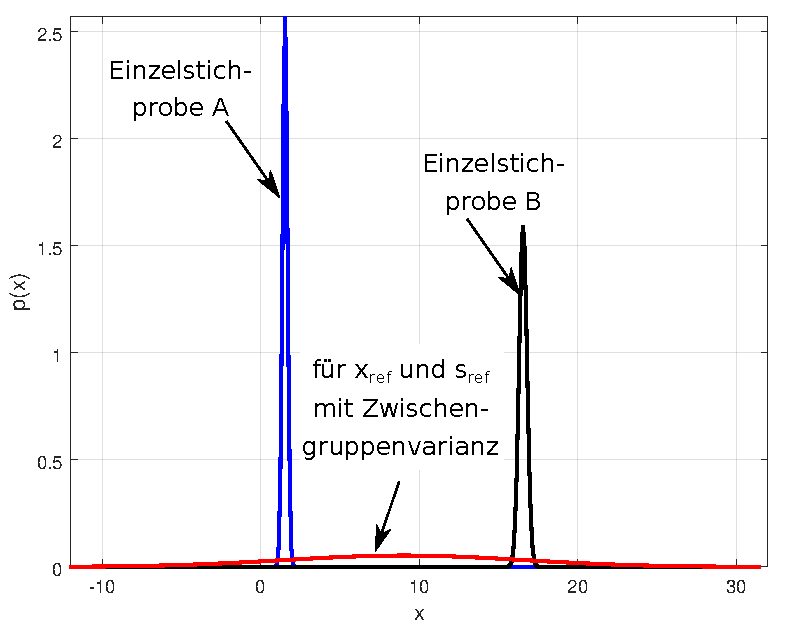
\includegraphics[width=120mm]{06_vorlesung/media/PauleMandel.pdf}
		\caption{Wahrscheinlichkeitsdichteverteilungen als Normalverteilungen
  zu Beispiel II mit blauer Kurve für die Einzelstichprobe A mit $\bar x_{II,A} = 1.533$
  und $\bar s_A = 0.1542$, schwarzer Kurve für die Einzelstichprobe B mit $\bar x_{II,B} = 16.550$
  und $\bar s_B = 0.2500$, sowie die gemeinsame Verteilung nach Hinzufügen der Zwischengruppenvarianz mit
  $x_\mathrm{ref} = 9.040$ und $\sqrt{\operatorname{Var}(x_\mathrm{ref})} = 7.5$ als sehr viel breitere und
  flachere Gaußverteilung dargestellt als rote Kurve.}
		\label{fig:Pau82BeispielII}
	\end{center}
\end{figure}

Der dazu gehörige Quellcode für Gnu-Octave/Matlab sieht wie folgt aus:
\begin{lstlisting}[style=Matlab]
function consensus_fit()
% Programm laeuft unter Matlab und Gnu-Octave
x_A = [2.0,1.0,1.5,1.8,1.2,1.7];
N_A = length(x_A);
x_B = [16.3,16.8];
N_B = length(x_B);

bar_x_A = mean(x_A);
bar_x_B = mean(x_B);
fprintf('Mittelwerte: %f und %f \n', bar_x_A, bar_x_B);

% Varianzen der Mittelwerte
Var_A_mittel = var(x_A)/N_A;
Var_B_mittel = var(x_B)/N_B;
fprintf('Varianzen der Mittelwerte innerhalb jeder Stichprobe: \n %f und %f \n'...
,  Var_A_mittel, Var_B_mittel);

% Anzahl der Methoden/ Partner M
M = 2;
% Startwert fuer Zwischengruppenvarianz
v_0 = 0;

% Berechnung des Birge ratio fuer den Startwert
w_A = 1/Var_A_mittel;
w_B = 1/Var_B_mittel;
x_ref = (w_A*bar_x_A + w_B*bar_x_B ) / (w_A + w_B);
RB = sqrt( (1/(M-1))*(w_A * (bar_x_A - x_ref)^2 + ...
w_B * (bar_x_B - x_ref)^2));
fprintf('Birge-Verhaeltnis fuer den Startwert %f\n\n',RB)
%
max_num_iterations = 50;
v = v_0;
k = 0;
while (RB > 1) && (k < max_num_iterations)
w_A = 1/(Var_A_mittel + v);
w_B = 1/(Var_B_mittel + v);

x_ref = (w_A*bar_x_A + w_B*bar_x_B ) / (w_A + w_B);
RBsq = (1/(M-1))*(w_A * (bar_x_A - x_ref)^2 + ...
w_B * (bar_x_B - x_ref)^2);
RB = sqrt(RBsq);
Q = RBsq - 1;
dQ_dv = (-1/(M-1))*(w_A^2 * (bar_x_A - x_ref)^2 + ...
w_B^2 * (bar_x_B - x_ref)^2);
dv = -Q / dQ_dv;
v = v + dv;
k = k + 1;
fprintf('x_ref: %f, RB: %.3f, dv: %e --> v: %.3f\n', x_ref, sqrt(RBsq), dv,v);
end
fprintf('\n s_b = %f bei Anzahl Iterationen %d\n', ...
sqrt(v-dv), k);
end
\end{lstlisting}
mit dem Output:
\begin{lstlisting}[style=Matlab]
>> consensus_fit
Mittelwerte: 1.533333 und 16.550000
Varianzen der Mittelwerte innerhalb jeder Stichprobe:
0.023778 und 0.062500
Birge-Verhaeltnis fuer den Startwert 51.123910

x_ref: 5.671861, RB: 51.124, dv: 4.312238e-02 --> v: 0.043
x_ref: 7.356441, RB: 36.154, dv: 8.619528e-02 --> v: 0.129
x_ref: 8.198732, RB: 25.569, dv: 1.721928e-01 --> v: 0.302
x_ref: 8.619877, RB: 18.087, dv: 3.435958e-01 --> v: 0.645
x_ref: 8.830449, RB: 12.799, dv: 6.840440e-01 --> v: 1.329
x_ref: 8.935734, RB: 9.064, dv: 1.355587e+00 --> v: 2.685
x_ref: 8.988376, RB: 6.429, dv: 2.661878e+00 --> v: 5.347
x_ref: 9.014695, RB: 4.574, dv: 5.132109e+00 --> v: 10.479
x_ref: 9.027851, RB: 3.273, dv: 9.539961e+00 --> v: 20.019
x_ref: 9.034421, RB: 2.371, dv: 1.649219e+01 --> v: 36.511
x_ref: 9.037690, RB: 1.756, dv: 2.470307e+01 --> v: 61.214
x_ref: 9.039294, RB: 1.357, dv: 2.797615e+01 --> v: 89.190
x_ref: 9.040038, RB: 1.124, dv: 1.861186e+01 --> v: 107.802
x_ref: 9.040319, RB: 1.022, dv: 4.691663e+00 --> v: 112.494
x_ref: 9.040375, RB: 1.001, dv: 2.129841e-01 --> v: 112.707
x_ref: 9.040377, RB: 1.000, dv: 4.038510e-04 --> v: 112.707
x_ref: 9.040377, RB: 1.000, dv: 1.446530e-09 --> v: 112.707
x_ref: 9.040377, RB: 1.000, dv: 0.000000e+00 --> v: 112.707

s_b = 10.616355 bei Anzahl Iterationen 18
\end{lstlisting}
%\nopagebreak
%\begin{thebibliography}{-----------}
%	\item[] \hspace*{5em}{\Large\bf zu Kapitel 6:}
%	\bibitem[Cox02]{6_Cox02} M. G. Cox: The evaluation of key comparison data, Metrologia 39, 589-595 (2002)
%	\bibitem[ISO13528]{6_ISO13528} ISO: Statistical methods for use in proficency testing by interlaboratory comparison, Second edition 2015-08-01, corrected version 2016-10-15
%	\bibitem[Kac08]{6_Kac08} R.N.Kacker, A.B.Forgbers
%	R. N. Kacker, A. B. Forbes, R. Kessel and K. Sommer Bayesian posterior predictive
%	p-value of statistical consistency in interlaboratory evaluations Metrologia 45 512-523 (2008)
%	\bibitem[GuideKey]{6_GuideKey} Guidelines for CCPR Key Comparison Report
%	Preparation, https://www.bipm.org/utils/common/pdf/CC/CCPR/CCPR-G2.pdf
%	\bibitem[Pau82]{6_Pau82}  R.C. Paule, J. Mandel: Consensus Values and Weighting Factors, J. Res. NBS, Vol.87, No.5,377-385 (1982)
%\end{thebibliography}

%
\chapter{Messunsicherheitsfortpflanzung bei linearen Modellen}
\label{unsicherheitsfortpfLin}
\section{Konzepte der Messunsicherheitsfortpflanzung (M.U.F.)}

% 1 Fortpflanzung für lineare Modelle
% 2 Überdeckungsintervall
% 3 Kombinierte Standardabweichung
%   (Sattherthwaite)
% 4 Erweiterungsfaktor

In der Messtechnik geht es darum, indirekte Messgrößen über Beobachtungen von direkten
Messgrößen und über ein Schätzverfahren auf Basis eines Modells zu ermitteln.
In der ersten Vorlesung hatten wir dazu hervorgehoben, dass zu dem Modell zum einen
die mathematische Beschreibung des physikalischen Sachverhaltes gehört und zum anderen
die statistische Beschreibung von nicht deterministischem Verhalten.
Das nichtdeterministische Verhalten eines Systems wird in vielen Fällen
von nicht vorhersehbaren, kleinen Störeinflüssen und Auflösungsbegrenzungen
beim Beobachtungsvorgang verursacht. Es gibt aber auch Prozesse, bei denen
der physikalische Vorgang, der zu untersuchen ist, selber stochastischen Charakter hat,
wie beispielsweise bei radioaktiven Zerfällen, Streuprozessen atomarer Vorgänge oder bei
biologischen Prozessen. Das nicht deterministische Verhalten, die
Stochastik, eines Prozesses wird mittels entsprechender Wahrscheinlichkeitsverteilungen modelliert.

Ein Messergebnis einer Größe $X$ wird deshalb statistisch mit Wahrscheinlichkeitsverteilungen ausgedrückt
\begin{itemize}
\item in Form einer Wahrscheinlichkeitsdichteverteilung
$$
p(X)
$$
oder
\item in Form der statistischen Momente, Erwartungswert $x$ und Varianz (bzw.\ deren Wurzel $\sigma_X$),
einer Wahrscheinlichkeitsdichteverteilung, zusammen mit einer Wahrscheinlichkeit $1-\alpha$
bzw.\ einem Quantil $k$
$$
x = \int X \, p(X) \operatorname d X, \quad
\sigma_X = \sqrt{\int (X-x)^2 \, p(X) \operatorname d X}, \quad k = P^{-1}(1-\alpha/2).
$$
\end{itemize}
Dreh- und Angelpunkt bei der Quantifizierung von Messgrößen ist die Vorgehensweise, wie ein
Mess\-er\-gebnis durch Modellbildung, Parameterschätzung und Bestimmung der Wahrscheinlichkeitsdichtefunktion
der Parameter gewonnen wird. Ein Messergebnis einer Größe $Y$ oder eines Größenvektors
$\mathbf{Y}$, die bzw.\ der \textsl{explizit} oder \textsl{implizit} von direkten
Messgrößen $\mathbf{X}$ abhängt, soll ausgedrückt werden durch eine
Wahrscheinlichkeitsdichteverteilung $p(Y)$ bzw.\ durch den entsprechenden Erwartungswert $y$ und
die Wurzel aus der Varianz $\sigma_Y$ mit einem Quantil $k$, dem Erweiterungsfaktor, für
eine spezifizierte Wahrscheinlichkeit $1-\alpha$.

Wir kategorisieren die Modelle für indirekte Messgrößen
danach, ob sie univariat oder multivariat und ob sie explizit oder implizit sind:

\begin{center}
{\setlength{\extrarowheight}{4pt}%
\begin{tabular}{l||c|c|}
\arraycolsep=4pt\def\arraystretch{2}
 & univariat: $1$ indirekte Größe & multivariat: $M>1$ indirekte Größen \\[4pt]
\hline\hline
explizit & $Y = f(\mathbf{X})$ & $\mathbf{Y} = \vec f(\mathbf{X})$\\[4pt]
\hline
implizit & $f(Y,\mathbf{X})=0$ & $f(\mathbf{Y},\mathbf{X})=0$ oder
 $\vec f(\mathbf{Y},\mathbf{X})=0$\\[4pt]
\hline
\end{tabular}}
\end{center}

mit $\mathbf{X} = (X_1,\dots,X_N)^\mathsf{T}$ und $\mathbf{Y} = (Y_1,\dots,Y_M)^\mathsf{T}$.

Bei der linearen Regression beispielsweise haben wir, wie wir es in der zweiten Vorlesung
gelernt haben, die Regressoren und Regressanden als
\begin{enumerate}
\item gemeinsam ausgelesene (z.B.\ durch Triggerung zugeordnete) Beobachtungstupel
\begin{equation}
\boldsymbol (Y_{\mathrm{Regr}, j}, \mathbf{X}_j) \; = \; (Y_{\mathrm{Regr}, j}, X_{1,j}, \dots, X_{M,j})
\end{equation}
vorliegen mit $j = 1,\dots, J$ und $J$ für den Stichprobenumfang, so dass gemäß einem
zeitlichen Ablauf eine Veränderung aller Größen vorliegen kann,
\item ansonsten können die direkten Messgrößen in voneinander unabhängigen Experimenten
und damit im allgemeinen auch mit verschiedenen Stichprobenumfängen gewonnen werden.
\end{enumerate}

Der erstere Fall repräsentiert als direkte Größen
sowohl die Regressoren $\mathbf{X}$ als auch die Regressanden $Y_{\mathrm{Regr}}$
und als indirekte Messgrößen, die Modellparameter $\boldsymbol \theta \equiv \boldsymbol Y$.
Hier handelt es sich also hinsichtlich der Unsicherheitsfortpflanzung um ein
implizites, multivariates Problem, auch bei der univariaten, linearen Regression.
\begin{equation}
0 = f(\mathbf{Y},\mathbf{X}) \equiv f(\boldsymbol \theta,\mathbf{X})
= Y_{\mathrm{Regr}} - \sum_{i=1}^{M} \theta_i \, X_i
\label{implizitMultivariatRegre}
\end{equation}
Das \glqq Multivariate\grqq ~für die Unsicherheitsberechnung betrifft die indirekten
Messgrößen $\boldsymbol \theta \equiv \boldsymbol Y$, das \glqq Univariate\grqq ~für die
Regression betrifft den Regressanden $Y_{\mathrm{Regr}}$.

Fall Zwei kann im allgemeinen so geartet sein, dass jede der direkten Größen in jeweils unabhängigen
Messvorgängen gewonnen wird, bei denen im allgemeinen unterschiedliche Stichprobenumfänge $J_i, J_k$ vorliegen
können und dann keine paarweise Zuordnung der einzelnen Beobachtungswerte $X_{i,j}$ zu $X_{k,l}$ für
$i \neq k$ vorliegt.

Bei dem expliziten, univariaten Fall
\begin{equation}
Y = f(\mathbf{X})
\label{explizitUnivariat}
\end{equation}
können die direkten Messgrößen als unkorrelierte unterschiedliche Stichproben vorliegen (Fall 2)
oder auch als gemeinsam getriggerte Tupel
\begin{equation}
\boldsymbol X_j \; = \; (X_{1,j}, \dots, X_{N,j})
\end{equation}
wie in Fall 1, aber dann nicht mit Regressionskoeffizienten als Modellparameter, sondern
mit der indirekten Größe explizit als Funktion von $(X_{1}, \dots, X_{N})$ gemäß
Gl.~(\ref{explizitUnivariat}).


Für eine internationale Vergleichbarkeit und den internationalen Handel ist es erforderlich,
dass die Verfahren zur Bestimmung von Messergebnissen möglichst einheitlich sind.
Für das gesetzliche Messwesen ist deshalb die international übereingekommene Richtlinie
zur Bestimmung von Messunsicherheiten bindend.
Die internationale Richtlinie zur Berechnung von Messunsicherheiten umfasst mehrere
Dokumente:
\begin{itemize}
\item JCGM 100:2008 GUM 1995 with minor corrections \textsl{Evaluation of measurement
data - Guide to the expression of uncertainty in measurement} \cite{GUM95}; oftmals einfach mit \glqq GUM\grqq ~bezeichnet,
betrifft univariate und explizite Modelle,
  \begin{itemize}
  \item die linear sind
  \begin{equation}
  Y = f(\mathbf{X}) = \sum_{i=1}^N c_i X_i
  \label{univarLinear}
  \end{equation}
  oder für die eine Linearisierung zulässig ist
  \begin{equation}
  Y = f(\mathbf{X})
  = \left. f(\mathbf{X}) \right|_{\bar{\mathbf{x}}} +
    \sum_{i=1}^N \underbrace{\left. \frac{\partial f}{\partial X_i} \right|_{\bar{\mathbf{x}}}}_{c_i} \Delta X_i
  \label{univarTaylorLin}
  \end{equation}
  \item die Zufallsgrößen betreffen, deren Streuung (\textsl{dispersion}) normalverteilt oder
  $t$-verteilt ist.
  \end{itemize}
Die indirekte Messgröße $Y$ ist damit Linearkombination der direkten Messgrößen $X_i$, d.h.
$Y = \sum c_i X_i$, so dass für die Varianz $\operatorname{Var}(Y) = \operatorname{Var}(\sum c_i X_i)$
gemäß Gl.~(\ref{univarLinearFortpflanzungKap1}) aus Abschnitt \ref{Kap1Kovarianzen} gilt
\begin{equation}
\operatorname{Var}(Y) = \sum_{i=1}^N \sum_{k=1}^N  c_i c_k \operatorname{Cov}(X_i, X_k)
\label{univarLinearFortpflanzung}
\end{equation}
Da sich viele physikalische Zusammenhänge für definierte Bereiche linearisieren lassen,
findet Gl.~(\ref{univarLinearFortpflanzung}) in großen Teilen der Messdatenanalyse
Anwendung und ist in der Literatur als das \textsl{Gesetz zur Fortpflanzung von Messunsicherheiten}
bekannt.

\item JCGM 101:2008 \textsl{Evaluation of measurement
data - Supplement 1 to the Guide to the expression of
uncertainty in measurement - Propagation of distributions using a Monte Carlo method} \cite{GUMS1};
kurz mit \glqq GUM - supplement 1\grqq ~bezeichnet, betrifft
explizite und implizite, univariate Modelle,
  \begin{itemize}
  \item die sich nicht einfach linearisieren lassen
  \item und/oder die sich nicht in einer geschlossenen analytischen Form darstellen lassen.
  \end{itemize}
Hier wird zu jeder direkten Messgröße eine Wahrscheinlichkeitsdichteverteilung vorgegeben.
Gemäß den jeweiligen Verteilungen wird eine große Stichprobe (ein großes \textsl{Sample})
$$
\mathbf{x}_1 = (x_{1,1},\dots,x_{N,1})^\mathsf{T}, \dots, \mathbf{x}_J = (x_{1,J},\dots,x_{N,J})^\mathsf{T}
$$
für die direkten Größen $\mathbf{X}$ per Zufallszahlengenerator erzeugt. Diese wird in das Modell $f$ gesteckt,
um eine Stichprobe
\begin{equation}
y_1 = f(x_{1,1},\dots,x_{N,1}), \dots, y_J = f(x_{1,J},\dots,x_{N,J})
\end{equation}
der indirekten Größe $Y$ zu gewinnen. Das Histogramm der Stichprobe der indirekten Größe liefert somit die
Wahrscheinlichkeitsdichteverteilung. Aus der sortierten Stichprobe nach der Art wie wir sie
für den Kolmogoroff-Smirnow-Test berechnet haben, gewinnen wir die kumulierte Wahrscheinlichkeitsverteilung
aus deren inverser Funktion das Überdeckungsintervall gewonnen werden kann.\\
$\rightarrow$ Dieses Verfahren wird Kapitel~\ref{montecarloMU} dargelegt.
\item JCGM 102:2011 \textsl{Evaluation of measurement data – Supplement 2 to the
Guide to the expression of uncertainty in measurement - Extension to any number of output quantities}
liefert die Verallgemeinerung der beiden Richtliniendokumente JCGM 100 und JCGM 101 für den multivariaten
Fall mit mehreren $M>1$ indirekten Größen, also einem Größenvektor $\mathbf{Y}$.
Hier wird dargelegt, wie man die Unsicherheit
  \begin{itemize}
  \item bei linearen oder linearisierbaren Modellen
    mittels der Berechnung der Kovarianzen (in der Art wie wir es
    in Kapitel~\ref{KapitellinReg} für die lineare Regression kennen gelernt haben)
  \item oder im Fall der nicht linearisierbaren und/oder komplexeren (oftmals impliziten) Modelle
    via Monte-Carlo-Berechnungen analog zu GUM-supplement 1
  \begin{equation}
  \mathbf{y}_1 = \vec f(x_{1,1},\dots,x_{N,1}), \dots, \mathbf{y}_J = \vec f(x_{1,J},\dots,x_{N,J})
  \end{equation}
  \item sowie für alle Fälle, ob uni- oder multivariat, ob explizit oder implizit, ob analytisch
    oder via Monte-Carlo-Verfahren unter Einbeziehung von {\`a} priori-Information mittels
    bayesischer Methoden\\
    $\rightarrow$ Kapitel~\ref{bayesMU}
  \end{itemize}
ermittelt.
\item JCGM 103 CD 2018-10-04 \textsl{Guide to the expression of uncertainty in measurement
- Developing and using measurement models} behandelt in umfassender Weise die Problematik der
Modellentwicklung. Es gibt den Bereich physikalischer, deterministischer Prozesse,
den Bereich der nicht-deterministischen, physikalischen oder biologischen oder soziologischen
Prozesse. Ferner gibt es den Bereich der statistischen Modelle, die dazu dienen, nicht-deterministische
Anteile von Prozessen zu behandeln. Das JCGM 103 Dokument soll diese Dinge konzeptionell
für die Metrologie beleuchten. Es ist bisher ein Entwurf; das Kürzel CD steht für \textsl{committee draft}.
\item JCGM 104:2009 \textsl{Guide to the expression of uncertainty in measurement
- An introduction to the Guide to the expression of
uncertainty in measurement and related documents} liefert die Konzepte und Hintergründe zur
Unsicherheitsbestimmung. Dieses Dokument soll ein Verständnis für die Konzepte der
Wahrscheinlichkeitsdichteverteilungen im Zusammenhang mit der Bestimmung von Messunsicherheiten liefern.
\item JCGM 106:2012 \textsl{Evaluation of measurement data - The role of
measurement uncertainty in conformity assessment}. Im Rahmen der Vorlesungen zu Hypothesentests und
Ringvergleichen haben wir bereits gelernt, dass Messergebnisse zu vergleichen sind, und wie dies
gehandhabt wird. In der Qualitätssicherung ist die zentrale Aufgabe, gefertigte Bauteile mit den
vorgegebenen Daten der technischen Konstruktionszeichnung zu vergleichen hinsichtlich der Übereinstimmung,
also der Einhaltung von Toleranzgrenzen. Dies wird Konformitätsbewertung genannt und wird im
JCGM 106-Dokument behandelt.
\end{itemize}

Das historisch älteste Dokument JCGM~100 gilt für explizite, univariate, skalare und
gauß- oder $t$-verteilte indirekte Messgrößen mit linearem oder linearisierbarem Modell für die
Abhängigkeit der indirekten Messgröße von den direkten Messgrößen. Es wurde zunächst erweitert durch das JCGM~101. Die
in JCGM~101 spezifizierte Monte-Carlo-Methode ermöglicht es, dass man nicht auf die Bestimmung der Unsicherheit
expliziter, univarter indirekter Messgrößen mit linearisierbarem Modell begrenzt ist.
Es bietet die Möglichkeit auch die Unsicherheit für implizite, multivariate Messgrößen,
deren direkte Eingangsgrößen beliebig verteilt sein können zu ermitteln. Die Verteilung der
Größen können eine von Null verschiedene Skewness aufweisen. Sie können sogar die Form einer
U-Verteilung haben, was beispielsweise bei direkten Größen, die durch Vibrationen beeinflusst
werden, vorkommen kann. Die Größen können irgendwelchen Verteilungen gehorchen, so dass die
Wahrscheinlichkeitsverteilungen der indirekten Messgrößen entsprechend einen
irgendwie gearteten Verlauf aufweisen können.

Die nächste Erweiterung liefert dann das JCGM~102-Dokument, das eine vollständige Verallgemeinerung
darstellt. Demgemäß werden auch Verfahren betrachtet, die die Berücksichtigung der Unsicherheit des Modells an sich
zulassen (die indirekte Messgröße aufgrund von Mangel an Information als Zufallsgröße behandelt)
sowie die Behandlung von vorherigen Informationen über die indirekten Messgrößen (Bayesische Statistik).

Die Dokumente JCGM 100, 101, 102, 104 und 106 sind über die Webseiten des
\textsl{Bureau International des Poids et Mesure}, abgekürzt BIPM,
\begin{verbatim}
https://www.bipm.org/en/publications/guides/#gum
\end{verbatim}
erhältlich.

Die wesentlichen Komponenten der Messunsicherheit sind
\begin{itemize}
\item die Begrenztheit des Messvorgangs bedingt durch
  \begin{itemize}
  \item endliche Auflösung der Geräte,
  \item Messbereichsgrenzen,
  \item Störeinflüsse von außerhalb und innerhalb der Geräte,
  \item subjektive Komponenten durch den Operateur,
  \end{itemize}
\item die Begrenztheit der Modellbildung bedingt durch
  \begin{itemize}
  \item Vereinfachungen (Parsimonie = \glqq Sparsamkeit\grqq)
    und Grenzen durch Rechenkapazität zeitlich (Rechenzeit/Rechenleistung)
    und kostenmäßig (Speicherkapazität und Maschinengenauigkeit,
    numerische Stabilität, numerische Zuverlässigkeit),
  \item Vereinfachungen mangels Kenntniss über quantitative Details
    zu Einflussgrößen
    oder genaueren Details der Physik innerhalb des
    betreffenden physikalischen Effektes,
  \item mangels Informationen zu genaueren Werten von Einflussgrößen der
    physikalischen Prozesse.
  \end{itemize}
\end{itemize}

Bei der Schätzung von Modellparametern (Quantifizierung der indirekten Messgrößen)
spielt vielfach die numerische Zuverlässigkeit des Optimierungsalgorithmus eine
wichtige Rolle. Wenn wir das Kosten\-funktions\-beispiel der Abbn.~\ref{LSoptiExample1NM} und \ref{LSoptiExample1Grad}
mit dem der Abb.~\ref{LSoptiExample1NM} in Kapitel~\ref{LSoptiExample1SinusRQS} vergleichen,
erkennen wir, dass die Modellparameter bei Abb.~\ref{LSoptiExample1NM} und \ref{LSoptiExample1Grad}
in etwa die gleiche Skalierung aufweisen, während die in Abb.~\ref{LSoptiExample1NM} stark unterschiedlich sind. In Abb.~\ref{LSoptiExample1NM} und \ref{LSoptiExample1Grad} sehen wir eine schöne, runde
Kuhle und in Abb.~\ref{LSoptiExample1Grad} einen schmalen Graben. Im letzteren ist das Modell mit seinen
Parametern nicht so gut konditioniert, so dass das Minimum nicht klar erkennbar ist.
Nicht so gut konditionierte Modelle führen eine größere Unsicherheit bei der Schätzung
seiner Parameter mit sich.

Für die Wahl des Modellansatzes gilt es nicht nur den physikalischen Zusammenhang
geeignet wieder zugeben, sondern auch das Verhalten der Gleitkommaarithmetik zu
berücksichtigen. Wenn zwei sehr große Zahlen voneinander zu subtrahieren sind, muss
berücksichtigt werden, wie hoch die Maschinengenauigkeit ist, also wie groß die
Mantisse ist. Werden die Zahlen so groß, dass die relevanten Nachkommastellen, die
nach Subtraktion gewonnen werden sollen, nicht vorhanden sind, liefert der Algorithmus
kein brauchbares Ergebnis.
\begin{quote}
Doing floating point operations is like moving piles of sand: every
time you move a pile, you lose a little sand and pick up a little dirt!
\end{quote}
Ein Algorithmus ist deshalb derart zu implementieren, dass hohe Potenzen oder
vielfache Multiplikationen vor Additionen oder Subtraktionen zu vermeiden, zu umgehen
sind. Dazu gehört es, zu überlegen, wie man das Modell formuliert, beispielsweise
ob man Polynome in der einfachen Darstellung, als Legendre oder als Tschebycheff-Polynome
definiert. Dazu gehört auch, zu prüfen, ob man und wie man ein Modell zunächst in einer
einfacheren Approximation aufbaut und erforderlichenfalls Effekte höherer Ordnung in
einem nächsten Schritt hinzufügt.

Ein Modell ist so zu wählen, dass es der entsprechenden Anwendung gerecht wird
hinsichtlich der Anforderungen an Kosten vs.\ Genauigkeit. Wie gut ein Modell einen
physikalischen Sachverhalt beschreibt, wird in der Modellunsicherheit ausgedrückt.
Ein kleines Beispiel hatten wir in Kapitel~\ref{KapitellinReg} gesehen, in der ein Vergleich
zwischen einer Regressiongeraden und einem Polynom 6.\ Grades gemacht wurde, siehe
dort das in Abb.~\ref{fig:LineareRegressionMoeglFits} dargestellte Beispiel.


\section{M.U.F. für univariate, explizite indirekte Größe, linear von direkten Größen abhängig}


In der ersten Vorlesung, in Abschnitt \ref{Kap1Kovarianzen}, wurden die Varianz und Kovarianz
von Zufallsgrößen eingeführt. In dem Zusammenhang haben wir die Rechenregeln für Erwartungswerte,
Summen, Produkte und Skalierungen dazu eingeführt. Auf Grundlage dieser Rechenregeln haben
wir die Varianz einer Zufallsgröße, die Linearkombination von mehreren Zufallsgrößen $X_i$ ist,
als Funktion der Kovarianzen der Zufallsgrößen $X_i$ bestimmt.
Wir wiederholen hier noch mal kurz die Herleitung zu Gl.~(\ref{univarLinearFortpflanzungKap1})
und damit also Gl.~(\ref{univarLinearFortpflanzung}) und zeigen,
weshalb die Varianz einer indirekten Größe, die linear
von den direkten Messgrößen gemäß Gl.~(\ref{univarLinear}) abhängt, Funktion der Kovarianzen
und Varianzen der direkten Messgrößen ist.

\begin{equation}
\operatorname {Var}\left(Y\right) \; = \;
\operatorname {Var}\left(\sum _{{i=1}}^{N}c_i X_{i}\right) \; = \;
\sum _{{i,k=1}}^{N}\operatorname {Cov}(c_i X_{i}, c_k X_{k}),
\label{eq:VarianzSummeISTSummeKovarianz}
\end{equation}
Mit
\begin{equation*}
\operatorname {Var}\left(\sum _{{i=1}}^{N}c_i X_{i}\right) \; = \;
\int\limits_{-\infty}^{\infty} \dots \int\limits_{-\infty}^{\infty}
\, \left[ \left(\sum_{i=1}^N c_i X_i\right) \; - \; E(\sum_{i=1}^N c_i X_i) \right]^2 \, p(X_1, \dots, X_N)
\, \operatorname{d}X_1 \dots \operatorname{d}X_N .
\end{equation*}
und
$$
\left(\sum_{i=1}^N c_i X_i \right) \; - \; E\left(\sum_{i=1}^N c_i X_i\right) \; = \;
\left(\sum_{i=1}^N c_i X_i \right) \; - \; \sum_{i=1}^N c_i E(X_i)
$$
gilt
\begin{equation}
\operatorname {Var}\left(\sum _{{i=1}}^{N}c_i X_{i}\right) \; = \;
\int\limits_{-\infty}^{\infty} \dots \int\limits_{-\infty}^{\infty}
\, \left[ \sum_{i=1}^N \left(c_i X_i \; - \; E(c_i X_i)\right) \right]^2 \, p(X_1, \dots, X_N)
\, \operatorname{d}X_1 \dots \operatorname{d}X_N .
\end{equation}
Mit Anwendung des Assoziativgesetzes gilt
\begin{equation*}
\operatorname {Var}\left(\sum _{{i=1}}^{N}c_i X_{i}\right) \; = \;
\int\limits_{-\infty}^{\infty} \dots \int\limits_{-\infty}^{\infty}
\, \sum_{i=1}^N \sum_{k=1}^N \, c_i \,  \left(X_i \; - \; E(X_i)\right) \;
      c_k \, \left(X_k \; - \; E(X_k)\right) \, p(X_1, \dots, X_N)
\, \operatorname{d}X_1 \dots \operatorname{d}X_N .
\end{equation*}
Durch Berechnung der Marginalverteilungen und weil $\int p(X_j) \, \operatorname{d}X_j = 1$
für alle $j$, die weder $i$ noch $k$ sind erhalten wir
\begin{equation}
\operatorname {Var}\left(\sum _{{i=1}}^{N}c_i X_{i}\right) \; = \;
\sum_{i=1}^N \sum_{k=1}^N  \;
\int\limits_{-\infty}^{\infty} \int\limits_{-\infty}^{\infty}
\, c_i \, \left(X_i \; - \; E(X_i)\right) \;
     c_k \, \left(X_k \; - \; E(X_k)\right) \, p(X_i, X_k)
\, \operatorname{d}X_i \operatorname{d}X_k .
\end{equation}
Der Term auf der rechten Seite ist genau die Kovarianz der beiden
Größen $X_i$ und $X_k$.

Mit der Definition der Kovarianz
$$
\operatorname {Cov}(X_{i},X_{k}) :=
\int\limits_{-\infty}^{\infty} \int\limits_{-\infty}^{\infty}
\, \left(X_i \; - \; E(X_i)\right) \;
      \left(X_k \; - \; E(X_k)\right) \, p(X_i, X_k)
\, \operatorname{d}X_i \operatorname{d}X_k
$$
erhalten wir das Fortpflanzungsgesetz in der Form, wie wir es aus Abschnitt \ref{Kap1Kovarianzen}
Gl.~(\ref{univarLinearFortpflanzungKap1}) bereits kennen gelernt haben.
\begin{equation}
{\begin{aligned}
\operatorname {Var}\left(Y\right) & =
\operatorname {Var}\left(\sum _{{i=1}}^{N} \, c_i \, X_{i}\right) \\
 & = \sum _{i=1}^{N}\sum _{k=1}^{N}\operatorname {Cov}(c_i X_{i}, c_k X_{k})\\
 & = \sum _{{i=1}}^{N} \, c_i^2 \, \operatorname {Var}(X_{i})+
     \sum _{{i,k=1,i\neq k}}^{N} \, c_i c_k \,  \operatorname {Cov}(X_{i},X_{k})\\
& = \sum _{{i=1}}^{N} \, c_i^2 \operatorname {Var}(X_{i})+2\sum _{{i=1}}^{{N-1}}
  \sum _{{k=i+1}}^{N} \, c_i c_k \operatorname {Cov}(X_{i},X_{k}).
\end{aligned}}
\label{univarLinearFortpflanzungKap7}
\end{equation}
Bei getrennter Betrachtung der beiden Terme mit den Varianzen $\operatorname {Var}(X_{i})$
und mit den Kovarianzen $\operatorname {Cov}(X_{i},X_{k})$, also
in der Notation $\sum \, c_i^2 \operatorname {Var}(X_{i})+2\sum
 \sum \, c_i c_k \operatorname {Cov}(X_{i},X_{k})$, wird deutlich, ob
die direkten Messgrößen korrelieren oder nicht.

Es gibt Anwendungen, bei denen die Korrelationkoeffizienten, definiert in
Abschnitt \ref{Kap1Kovarianzen} Gl.~(\ref{KorrelationskoeffizientKap1})
$\rho_{i,k} = \frac{\operatorname {Cov}(X_{i},X_{k})}{\sqrt{\operatorname {Var}(X_{i}) \operatorname {Var}(X_{k})}}$,
angegeben werden und die Standardabweichungen $\sigma_i = \sqrt{\operatorname {Var}(X_{i})}$, so dass
das Unsicherheitsfortpflanzungsgesetz auch in dieser Form aufgeschrieben wird
\begin{equation}
\operatorname {Var}\left(Y\right) = \sigma_Y^2  =
\sum _{{i=1}}^{N} \, c_i^2 \sigma_i^2 \, + \, 2\sum _{{i=1}}^{{N-1}}
  \sum _{{k=i+1}}^{N} \, c_i c_k \rho_{i,k} \sigma_i \sigma_k .
\label{FortpflaKorrStd}
\end{equation}

Die aus dem Fortpflanzungsgesetz resultierende Messunsicherheit $\sigma_Y$ wird auch
\textsl{kombinierte Standardabweichung} genannt.

Oftmals, so auch im \textsl{Guide} für Messunsicherheit GUM - JCGM 100, wird anstelle der
Bezeichnung $\rho_{i,k}$ die
Bezeichnung $r(X_{i},X_{k})$ verwendet, meint aber dasselbe.

Alternativ, insbesondere im GUM - JCGM 100, gibt es die Schreibweise mit $u$ anstelle der
Standardabweichungen $\sigma$ als Kürzel für \textsl{uncertainty} oder \textsl{Unsicherheit},
und heißt in diesem Zusammenhang \textsl{Standardunsicherheit} (engl.\ \textsl{standard uncertainty}).
Dabei können je nach Anwendung mit den Standardabweichungen $\sigma$ Standardabweichungen je einer
Einzelstichprobe sein, oder - was häufiger vorkommt - Standardabweichungen der Mittelwerte der Stichproben
zu den jeweiligen Messgrößen:

\begin{equation}
{\begin{aligned}
u^2(Y) & = \sum\limits_{i=1}^{N} \, c_i^2 \operatorname {Var}(X_{i}) \; + \; 2 \, \sum _{{i=1}}^{{N-1}}
  \sum\limits_{k=i+1}^{N} \, c_i \, c_k \operatorname {Cov}(X_{i},X_{k})\\
 & = \underbrace{\sum\limits_{i=1}^{N} \, c_i^2 \, u^2(X_i)}_{\mathrm{unkorrelierter~Fall}} \;  + \;
 \underbrace{2 \, \sum\limits_{i=1}^{{N-1}}
 \sum\limits_{k=i+1}^{N} \, c_i \, c_k \, \rho_{i,k} \, u(X_i) \, u(X_k)}_{\mathrm{Mischterme:~korrelierter~Fall}} .
\end{aligned}}
\label{UnsichFortpfl2}
\end{equation}
mit
\begin{equation}
\operatorname{Cov}(X_i, X_i) \; \equiv \; \operatorname{Var}(X_i)
\; \equiv \; \sigma^2_i \; \equiv \;  u^2(X_i)
\end{equation}
und
\begin{equation}
\operatorname{Cov}(X_i, X_k) \; \equiv \;
\sigma_{i,k} \; \equiv \; u(X_i,X_k)
\end{equation}
Hier sind keine Tippfehler bezüglich der Quadrate, es gilt tatsächlich $u^2(X_i) = u(X_i,X_i)$ für die Varianzen
sowie $\sigma^2(X_i) = \sigma(X_i,X_i)$ für die Kovarianzen.

Im JCGM 100-Dokument des \textsl{Guide} für Messunsicherheit GUM in Absatz 5.2.4
werden als typische Ursachen für die Korrelation von Eingangsgrößen  folgende aufgeführt:
\begin{itemize}
\item Verwendung desselben Normals (Prüfkörpers) oder Messgeräts;
\item Verwendung mehrerer Normale, die in derselben Vorrichtung kalibriert
wurden (z.B. gestückelte Masse-Normale bei der Kalibrierung einer Waage);
\item Verwendung des gleichen Referenzwertes;
\item Eine Eingangsgröße hängt direkt von einer weiteren ab
(z.B. Luftdruck von Um\-geb\-ungs\-tem\-pe\-ra\-tur);
\item Zwei oder mehr Eingangsgrößen sind von
demselben Effekt beeinflusst
(z.B. Stromstärke und Spannung in einem Messkreis, so dass beide
von Schwankungen der Stromquelle beeinflusst werden).
\end{itemize}

Bei gemeinsam aufgenommenen Tupeln direkter Messgrößen (z.B.\ Stromstärke und Spannung in
einem Messkreis), die miteinander korreliert sein können, sieht die Kovarianz aufgrund
der Zuordnung mit gemeinsamer Beobachtung (Ziehung) jeweils eines Tupels $\mathrm{X}_j$ wie folgt aus:
$$
\operatorname{Cov}(X_i, X_k) \, = \,
\frac{1}{J-1} \sum_{j=1}^J (X_{i,j} - \bar x_i) (X_{k,j} - \bar x_k)
 \quad \mathrm{und~mit}
\quad  \bar x_i \, = \, \frac{1}{J} \sum_{j=1}^J X_{i,j}
$$
für $i,k = 1,\dots, N$.

Bei den aufgelisteten Fällen, bei denen es keine direkte Zuordnung von Beobachtungen
der verschiedenen direkten Messgrößen gibt, wie es bei der Verwendung desselben Normals oder
Messgeräts sein kann, erfordert die Abschätzung eines Korrelationskoeffizienten
$\rho$ oder $r$ eine geeignete Modellbildung.


\section{M.U.F. für univariate, explizite indirekte Größe, Abhängigkeit von direkten Größen linearisierbar}

Zunächst beleuchten wir ein Beispiel, bei dem ein Modellparameter $Y$ berechnet wird,
der sich aus dem Produkt zweier direkter
Messgrößen $X_1$ und $X_2$ ergibt. Wir beschäftigen uns mit dem Fall, dass
die beiden direkten Größen nicht von einander abhängen. Sie sollen zwei unterschiedlichen
und unabhängigen Grundgesamtheiten angehören, d.h.\ unkorreliert sein.

Das Modell sei
\begin{equation}
Y \; = \; X_1 \, X_2
\label{BeispielProdukt2Gr}
\end{equation}
und es wurden zu jeder der beiden direkten Größen zu unterschiedlichen Zeiten unterschiedlich
große Stichproben gezogen.

Die naheliegende Vorgehensweise ist nun, die Mittelwerte der beiden Stichproben zu berechnen und
diese miteinander zu multiplizieren
\begin{equation}
y \; = \; \left(\frac{1}{J_1} \sum_{j=1}^{J_1} X_{1,j}\right) \,
          \left(\frac{1}{J_2} \sum_{j=1}^{J_2} X_{2,j}\right) .
\end{equation}
Für die Berechnung der kombinierten Standardabweichung von $Y$ bestimmen wir
die Standardabweichungen $s_i$ der beiden Stichproben $i = 1,2$ zu den Größen $X_1$ und $X_2$:
\begin{equation}
s_i \; = \; \sqrt{ \frac{1}{J_i - 1} \sum_{k=1}^{J_i}
 \left( X_{i,k} \; - \; \frac{1}{J_i} \sum_{j=1}^{J_i} X_{i,j}\right)^2 }
\end{equation}
Wir betrachten die Empfindlichkeit der Modellfunktion, wie stark die Größe $Y$ auf
Abweichungen/ Veränderungen der Größen $X_1$ und $X_2$ reagiert.
In diesem Beispiel ist es sehr einfach, wenn die Größe $X_1$ um $\Delta X_1$ verschoben wird
\begin{equation}
Y + \Delta Y \; = \; (X_1 + \Delta X_1) \, X_2 \; = \; X_1\, X_2 + \Delta X_1 \, X_2
\end{equation}
dann ist
\begin{equation}
\Delta Y \; = \; \Delta X_1 \, X_2
\end{equation}
weil $Y$ linear von $X_1$ abhängt und es gilt
\begin{equation}
c_1 \; := \; \frac{\Delta Y}{\Delta X_1} \; = \; X_2
\end{equation}
was die Empfindlichkeit, d.h.\ Sensitivität $c_1$, der Größe $Y$ auf Änderungen der Größe
$X_1$ genannt wird.
\begin{figure}
\begin{center}
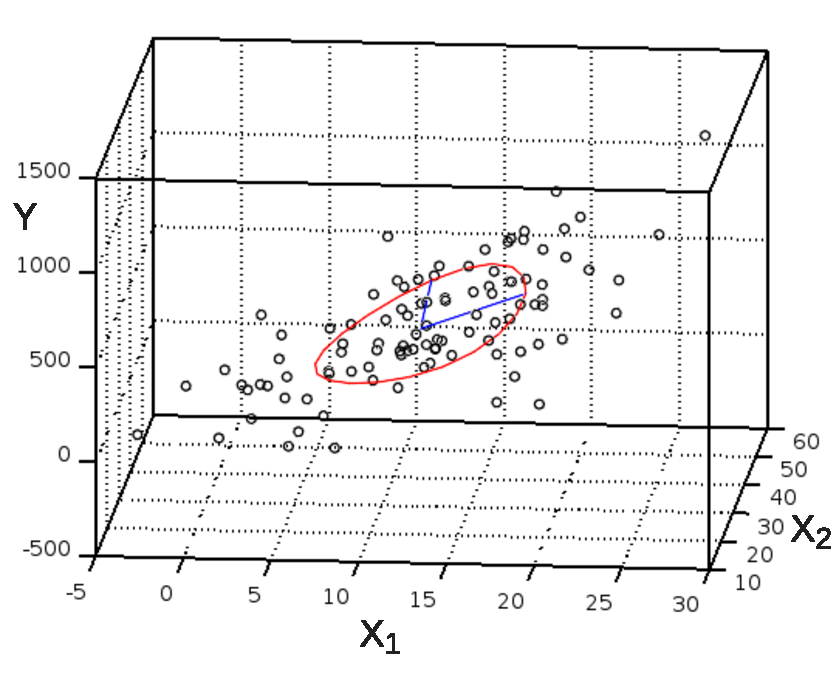
\includegraphics[width=100mm]{07_vorlesung/media/understand_fehlerfort_1.pdf}
\caption{\label{FortpfElliptisch} Eine anschauliche Deutung für die pythagoräische
Addition der Standardabweichungen liefert die Betrachtung der mit roter Kurve dargestellten
Ellipse. Die blauen Geraden repräsentieren die Abstände vom Mittelpunkt als Halbmesser
der Ellipse, die aus den Standardabweichungen jeweils von $X_1$ und $X_2$ berechnet wurden.}
\end{center}
\end{figure}
Da die beiden Größen $X_1$ und $X_2$ zwei unabhängige Dimensionen repräsentieren, werden
ihre Standardabweichungen nach dem Satz des Pythagoras addiert, eine Veranschaulichung dieses
Sachverhalts zeigt Abb.~\ref{FortpfElliptisch}. Da die Größen über die Modellgleichung
miteinander verknüpft sind und die gesuchte Standardabweichung die Dimension der Größe $Y$
trägt, müssen die Standardabweichungen der Größen $X_1$ und $X_2$ mit den entsprechenden
Sensitivitäten verknüpft werden, so dass
\begin{equation}
s_y^2 \; = \; (c_1 \, s_1)^2 \; + \; (c_2 \, s_2)^2 .
\end{equation}
Diese Varianz $s_y^2$ ist also wieder eine \textsl{kombinierte Varianz} und deren Wurzel
$s_y$ eine \textsl{kombinierte Standardabweichung}.

Für den allgemeinen Fall mit einer Linearsierung durch die Taylorreihenentwicklung
Gl.~(\ref{univarTaylorLin}) stellen die partiellen Ableitungen an
der Stelle der Schätzer der direkten Größen die Sensitivitäten
$c_i = \left. \frac{\partial f}{\partial X_i} \right|_{\bar{\mathbf{x}}}$ dar. Der
Vektor der partiellen Ableitungen heißt \textsl{Gradient}. Der Gradient ist also
der Steigungsvektor.
Der Gradient drückt aus, wie stark sich die indirekte Größe $Y$ gemäß der Steigung
des Kurvenverlaufs des Modells
ändert, wenn es kleine Änderungen der direkten Größen gibt. Mit anderen Worten besagt dies, wie
empfindlich die indirekte Größe auf Änderungen der direkten Größen reagiert, d.h.\ wie sensistiv
das Modell an der Position $\bar{\mathbf{x}}$ ist.

Gegeben sei ein univariates, expliziten Modell $Y = f(\mathrm{X})$, das linearisierbar ist, also
in Taylorreihe entwickelbar bis zum linearen Term mit dem Erwartungswertevektor
$\bar{\mathbf{x}}$ als Entwicklungspunkt
\begin{equation}
Y = f(\mathbf{X}) \approx \left. f(\mathbf{X}) \right|_{\bar{\mathbf{x}}} +
\sum_{i=1}^N \left.
\frac{\partial f}{\partial X_i} \right|_{\bar{\mathbf{x}}} \Delta X_i
\quad \text{und} \quad \mathrm{X} = \bar{\mathbf{x}} + \Delta \mathrm{X} .
\label{linearisiertesModellY}
\end{equation}
Die direkten Messgrößen $X_i$ sind Zufallsgrößen.
Bei der Linearisierung nehmen die Abweichungen $\Delta X_i$ der direkten Größen von ihren Erwartungswerten
$\mathrm{E}(X_i) = \bar x_i$ oder als Vektor mit den Erwartungswerten aller direkten Größen
$\bar{\mathbf{x}}$ die Rolle der Zufallsgrößen ein. Ihr Erwartungswert ist dann
Null $\mathrm{E}(\Delta X_i) = 0$.

Der Erwartungswert der indirekten Messgröße $Y$ wird durch Einsetzten der Erwartungswerte der
direkten Messgrößen in die Modellgleichung $Y = f(\mathrm{X})$ gewonnen
\begin{equation}
\mathrm{E}(Y) = \left. f(\mathbf{X}) \right|_{\bar{\mathbf{x}}}
\end{equation}

Zu der indirekten Messgröße soll die Varianz ermittelt werden
\begin{equation}
\operatorname{Var}(Y) =
\int \left(Y - E(Y) \right)^2 p(Y) \mathrm{d}Y =
\int \left(Y^2 - 2 Y \mathrm{E}(Y) + \mathrm{E}(Y)^2\right)  p(Y) \mathrm{d}Y
\end{equation}
mit $\int Y \mathrm{E}(Y) p(Y) \mathrm{d}Y = E(Y) \int Y p(Y) \mathrm{d}Y =
\mathrm{E}(Y) \mathrm{E}(Y)$ wird dies zu
\begin{equation*}
\operatorname{Var}(Y)
= \int \left(Y^2 - \mathrm{E}(Y)^2\right)  p(Y) \mathrm{d}Y
= \left(\int Y^2 p(Y) \mathrm{d}Y \right) - \mathrm{E}(Y)^2,
\end{equation*}
so dass gilt
\begin{equation}
\operatorname{Var}(Y)
= \int \left(Y^2 - \mathrm{E}(Y)^2\right)  p(Y) \mathrm{d}Y
= \int Y^2 p(Y) \mathrm{d}Y - \int \mathrm{E}(Y)^2  p(Y) \mathrm{d}Y .
\end{equation}
Hier wird der Ansatz Gl.~(\ref{linearisiertesModellY}) eingesetzt und mit
$p(Y)$ aus $p(X_1,\dots,X_N) = p(\mathbf{X})$ und mit
$\mathrm{d} \mathbf{X} = \mathrm{d} X_1\dots \mathrm{d} X_N$,
sowie mit $\int \mathrm{E}(Y)^2  p(Y) \mathrm{d}Y = \mathrm{E}(Y)^2$
\begin{equation}
\operatorname{Var}(Y)
= \int \left( \left. f(\mathbf{X}) \right|_{\bar{\mathbf{x}}} +
\sum_{i=1}^N \left.
\frac{\partial f}{\partial X_i} \right|_{\bar{\mathbf{x}}} \Delta X_i
 \right)^2
p(\mathbf{X}) \mathrm{d} \mathbf{X}
 \; - \; \mathrm{E}(Y)^2
\end{equation}
%\begin{small}
\begin{equation*}
= \int \left[ \left. f(\mathbf{X}) \right|_{\bar{\mathbf{x}}}^2 +
2   \left. f(\mathbf{X}) \right|_{\bar{\mathbf{x}}}
\sum_{i=1}^N \left.
\frac{\partial f}{\partial X_i} \right|_{\bar{\mathbf{x}}} \Delta X_i
+ \left(
\sum_{i=1}^N \left.
\frac{\partial f}{\partial X_i} \right|_{\bar{\mathbf{x}}} \Delta X_i
 \right)^2 \right]  p(\mathbf{X}) \mathrm{d} \mathbf{X}
\; - \mathrm{E}(Y)^2
\end{equation*}
%\end{small}
\begin{equation*}
= \int \left[
2   \left. f(\mathbf{X}) \right|_{\bar{\mathbf{x}}}
\sum_{i=1}^N \left.
\frac{\partial f}{\partial X_i} \right|_{\bar{\mathbf{x}}} \Delta X_i
+ \left(
\sum_{i=1}^N \left.
\frac{\partial f}{\partial X_i} \right|_{\bar{\mathbf{x}}} \Delta X_i
 \right)^2
\right]  p(\mathbf{X}) \mathrm{d} \mathbf{X}
\end{equation*}

\begin{equation*}
\operatorname{Var}(Y)
= \int \left[
2   \left. f(\mathbf{X}) \right|_{\bar{\mathbf{x}}}
\sum_{i=1}^N \left.
\frac{\partial f}{\partial X_i} \right|_{\bar{\mathbf{x}}} \Delta X_i
+ \left(
\sum_{i=1}^N \left.
\frac{\partial f}{\partial X_i} \right|_{\bar{\mathbf{x}}} \Delta X_i
 \right)^2
\right]  p(\mathbf{X}) \mathrm{d} \mathbf{X}
\end{equation*}
\begin{equation*}
= 2 \int   \left. f(\mathbf{X}) \right|_{\bar{\mathbf{x}}}
\sum_{i=1}^N \left.
\frac{\partial f}{\partial X_i} \right|_{\bar{\mathbf{x}}} \Delta X_i
\,  p(\mathbf{X}) \mathrm{d} \mathbf{X}
+ \int \left(
\sum_{i=1}^N \left.
\frac{\partial f}{\partial X_i} \right|_{\bar{\mathbf{x}}} \Delta X_i
 \right)^2
 p(\mathbf{X}) \mathrm{d} \mathbf{X}
\end{equation*}
\begin{equation*}
= 2 \left. f(\mathbf{X}) \right|_{\bar{\mathbf{x}}}  \sum_{i=1}^N \left.
\frac{\partial f}{\partial X_i} \right|_{\bar{\mathbf{x}}}
\underbrace{\int  \Delta X_i \, p(\mathbf{X}) \mathrm{d} \mathbf{X}}_{= 0}
+ \int \left(
\sum_{i=1}^N \left.
\frac{\partial f}{\partial X_i} \right|_{\bar{\mathbf{x}}} \Delta X_i
 \right)^2
 p(\mathbf{X}) \mathrm{d} \mathbf{X}
\end{equation*}

\begin{equation}
\operatorname{Var}(Y)
=
\int \left(
\sum_{i=1}^N \left.
\frac{\partial f}{\partial X_i} \right|_{\bar{\mathbf{x}}} \Delta X_i
 \right)^2
 p(\mathbf{X}) \mathrm{d} \mathbf{X}
=
\operatorname{Var}\left(\sum_{i=1}^N \left. \frac{\partial f}{\partial X_i} \right|_{\bar{\mathbf{x}}} \Delta X_i\right)
\end{equation}

Als nächstes wollen wir wieder das Fortpflanzungsgesetz für die Messunsicherheit
in der Gestalt von Gl.~(\ref{univarLinearFortpflanzungKap7}) erhalten, wobei jetzt die Koeffizienten
$c_i$ die Steigungen der Tangenten $\frac{\partial f}{\partial X_i}$ an der Stelle
der geschätzten Erwartungswerte sind, d.h.\
$c_i = \left. \frac{\partial f}{\partial X_i} \right|_{\bar{\mathbf{x}}}$

\begin{equation}
\operatorname{Var}(Y)
= \operatorname{Var}\left(\sum_{i=1}^N c_i \Delta X_i\right)
\end{equation}
\begin{equation}
\operatorname {Var}\left(Y\right)
= \sum _{{i=1}}^{N} \, c_i^2 \operatorname {Var}(\Delta X_{i})+2\sum _{{i=1}}^{{N-1}}
  \sum _{{k=i+1}}^{N} \, c_i c_k \operatorname {Cov}(\Delta X_{i},\Delta X_{k})
\label{UnsicherFortpflLinearisiert}
\end{equation}

Zu Kapitel 5.2 im JCGM 100-Dokument des \textsl{Guide} für Messunsicherheit GUM
sei angemerkt, dass für die Sensitivitäten eine verkürzte, unmathematische Schreibweise
für die Sensitivitäten gewählt wurde, indem dort geschrieben steht $\frac{\partial f}{\partial x_i}$
anstelle von $\left. \frac{\partial f}{\partial X_i} \right|_{\bar{\mathbf{x}}}$ oder
$\left. \frac{\partial f}{\partial X_i} \right|_{\bar x_1, \dots, \bar x_N}$.
Im GUM wird angemerkt, dass die saloppe Notation $\frac{\partial f}{\partial x_i}$ für
$\frac{\partial f}{\partial X_i}$
unter Verwendung der Schätzwerte $x_i$ zu den $X_i$ gewählt wird.
In unserer Vorlesungsreihe sowie im GUM steht das Symbol mit dem großgeschriebenen $X_i$ für die
direkten Messgrößen. Das im GUM verwendete $x_i$ als Kleinbuchstabe steht für den Schätzwert,
was wir in der Vorlesung mit $\bar x_i$ bezeichnen. Da der Schätzwert eine Konstante ist,
kann man nach dieser natürlich nicht ableiten.


\section{Überdeckungsintervall für indirekte Messgrößen}

Am Ende von Kapitel~\ref{konzepteStatistik} haben wir das Überdeckungsintervall eingeführt
und nach Einführung der Quantile der t-Verteilung in Kapitel~\ref{wahrscheinlichHyp} genauer
behandelt, als \textsl{Vertrauensintervall}, sowie im Zusammenhang der bayesischen Statistik
gewonnen aus der inversen kumulierten Posteriorverteilung als \textsl{Credible intervall}.

Die Intervallgrenzen des Vertrauensintervalls haben wir
auch als Produkt aus einem Quantil und einer Standardabweichung repräsentiert, im Fall, dass
eine Normalverteilung zugrunde gelegt wird in der Form
\begin{equation}
\left[\bar x \, - \, z_{1-\frac{1}{2}\alpha} \, \sigma_X,
\bar x \, + \, z_{1-\frac{1}{2}\alpha} \, \sigma_X \right]
\end{equation}
und im Fall, dass eine $t$-Verteilung zugrunde gelegt wird
\begin{equation}
\left[\bar x \, - \, t_{1-\frac{1}{2}\alpha, \nu} \, \sigma_X,
\bar x \, + \, t_{1-\frac{1}{2}\alpha, \nu} \, \sigma_X \right] .
\end{equation}
Bei dem Fall, dass eine $t$-Verteilung zugrunde gelegt wird, und zwar, wenn es um kleinere
Stichprobenumfänge geht, hängt das Quantil von der Anzahl der Freiheitsgrade $\nu_i = J_i - 1$
ab, die jedoch im allgemeinen für die beiden Größen $X_i$
unterschiedlich sein kann. Es gilt also, ein gemeinsames Quantil zu finden.

Mit der bayesischen Methode, die wir zuvor betrachtet haben, konnten wir das
\textsl{Credible Interval} aus der kumulierten Posterior gewinnen. Bei dem
zuvor erörterten Beispiel Gl.~(\ref{BeispielProdukt2Gr}) $Y = X_1 X_2$ haben wir statt
der einen Likelihood drei Verteilungsdichten:
Für jede Größe $X_i$ haben wir je eine Likelihood
\begin{equation}
p_{\mathrm{L},i}(\{X_{i,1}, \dots, X_{i,J}\} | X_i, s_i) \; = \;
\prod\limits_{j=1}^J \frac{1}{\sqrt{2 \pi} \, s_i}
 e^{- \frac{1}{2} \, \left( \frac{X_{i,j} - X_i}{s_i} \right)^2 }  \; = \;
l(X_i, s_i | \{X_{i,1}, \dots, X_{i,J}\})
\end{equation}
was zwei Verteilungen liefert, und als dritte Verteilung noch
\begin{equation}
p_\mathrm{L,y}( X_1, X_2 | Y, s) \; = \;
\frac{1}{\sqrt{2 \pi} \, s}
 e^{- \frac{1}{2} \, \left( \frac{Y - X_1 \, X_2}{s} \right)^2 }
\end{equation}
wobei dann nicht nur über $s$, sondern auch über $X_1$ und $X_2$ integriert wird, um die
Posterior als Marginalverteilung, die nur noch von $Y$ abhängt, zu erhalten.

Für relativ einfache analytische Zusammenhänge, also für explizite Modelle
und für ein\-fachere implizite Modellansätze wie die lineare Regression, ist
es nicht erforderlich die numerisch aufwendigere
kolmogoroff'sche Wahrscheinlichkeitsrechnung (Bildung
der Produkte der Verteilungen) anzuwenden.
Für explizite linearisierbare Modelle
$$
Y = f(\mathbf{X}) \qquad \mathbf{Y} = \vec f(\mathbf{X})
$$
mit $\vec f = (f_1,\dots,f_l, \dots, f_M)^\mathsf{T}$ ist das
Fortpflanzungsgesetz gemäß Gl.~(\ref{UnsichFortpfl2}) wie folgt
\begin{equation}
u^2(Y_l) = \sum\limits_{i=1}^{N} \, \left( \left. \frac{\partial f_l(\mathbf{X})}{\partial X_i}\right|_{\bar{\mathbf{x}}} \right)^2 \, u^2(X_i) \;  + \;
2 \, \sum\limits_{i=1}^{{N-1}}
 \sum\limits_{k=i+1}^{N} \, \left. \frac{\partial f_l(\mathbf{X})}{\partial X_i}\right|_{\bar{\mathbf{x}}} \,
 \left. \frac{\partial f_l(\mathbf{X})}{\partial X_k}\right|_{\bar{\mathbf{x}}}  \; \rho_{i,k} \, u(X_i) \, u(X_k)
\end{equation}
verwendbar. Für die lineare Regression
$$
Y_\mathrm{Regr} = \sum_{l=1}^M \theta_i X_l
$$
die bzgl.\ der indirekten Messgrößen $\theta_l = Y_l$ ein implizites Modell ist, gilt
für die Unsicherheitsfortpflanzung, die in Abschnitt~\ref{subsec:vertrauensbereiche}
dargelegt wird, siehe Gl.~(\ref{eq:Varianz des Achsenabschnitts}) bzw.\
Gl.~(\ref{eq:CovRegressparamsMatrix}) mit Gl.~(\ref{eq:URegressparamsMatrix}).
Mit einer Stichprobe mit Tupeln $(Y_{\mathrm{Regr},j}, X_{1,j},\dots,X_{M,j})$ und mit
$\boldsymbol Y_{\mathrm{Regr}} = (Y_{\mathrm{Regr},1},\dots,Y_{\mathrm{Regr},J})^{\mathsf{T}}$
und der Regressormatrix $\boldsymbol X = (X_{l,j})$ liefert das Fortpflanzungsgesetz die
Kovarianz der Modellparameter
\begin{equation}
\operatorname{Cov}(\boldsymbol \theta) \; = \; \left(\boldsymbol X^\mathsf{T} \, \boldsymbol X\right)^{-1} \, \operatorname{Var}(\boldsymbol \varepsilon)
\end{equation}
mit $J$ für den Stichprobenumfang und $M$ für die Anzahl der Modellparameter und mit
\begin{equation}
\operatorname{Var}(\boldsymbol \varepsilon) \; = \;
	\frac{1}{J-M}\left(\boldsymbol Y \; - \; \boldsymbol X \, \hat{\boldsymbol \theta}\right)^\mathsf{T}
\left(\boldsymbol Y \; - \; \boldsymbol X \, \hat{\boldsymbol \theta}\right) .
\end{equation}
Die Hauptdiagonale der Kovarianz der Modellparameter enthält die Varianzen
$$
\sigma_{\theta_l}^2 = u^2(\theta_l\equiv Y_l)
$$
der jeweiligen Modellparameter.

Für die Ermittlung des Überdeckungsintervalls $[y_l-U(Y_l), y_l+U_l]$ wird ein entsprechender
Erweiterungsfaktor $k$ für $U(Y_l) = k \, u(Y_l)$ gebraucht. Wird als Erweiterungsfaktor das
Quantil der $t$-Verteilung eingesetzt, so wird eine \textsl{effektive Anzahl
von Freiheitsgraden} $\nu_\mathrm{eff}$ approximiert.
In Abschnitt G.4 des Dokuments JCGM 100 GUM:2008 wird auf die Berechnungsmethode
für $\nu_\mathrm{eff}$ von Satterthwaite aus dem Jahr 1941 \cite{Sat41} zurückgegriffen.

Satterthwaite betrachtet die Varianz $\operatorname{Var}(s_i^2)$
der Varianz $s_i^2$. Die Varianzen $s_i^2$ sind unabhängige
Zufallsgrößen, also als Größen zu betrachten, die unkorreliert sind, so dass
\begin{equation}
\operatorname{Var}(s_y^2) \; = \;  \operatorname{Var}\left( c_1^2 s_1^2 \right)
 \; + \; \operatorname{Var}\left( c_2^2 s_2^2 \right)
\label{VarianzvarianzSumme}
\end{equation}
gilt.
Die empirischen Varianzen $s_1^2$ und $s_2^2$ der Größen $X_1$ und $X_2$ sind $\chi^2$-verteilt,
d.h.\ für die normierte Größe gilt
\begin{equation}
Q_i \; = \; \nu_i \, \left(\frac{s_i}{\sigma_i}\right)^2 \, \sim \; \chi^2(\nu_i) .
\end{equation}
Der Erwartungswert für $Q_i$ ist
\begin{equation}
\operatorname{E}(Q_i) \; = \; \int_0^\infty \; Q \; p_{\chi^2}(Q) \; \operatorname{d}Q \; = \; \nu_i.
\label{ErwartungswertQ}
\end{equation}
Die Varianz $\operatorname{Var}(Q_i)$ ist
\begin{equation}
\operatorname{Var}(Q_i) \; = \; \int_0^\infty \; (Q - \nu_i)^2 \; p_{\chi^2}(Q) \; \operatorname{d}Q \; = \; 2 \nu_i.
\label{VarianzQ}
\end{equation}
Die Herleitungen zu den beiden Gln.~(\ref{ErwartungswertQ}) und (\ref{VarianzQ})
befinden sich in Anhang \ref{ErwaChi2}.

Ferner gilt allgemein für die Varianz einer Zufallszahl $R$
multipliziert mit einem konstanten Faktor $a$
\begin{equation}
\arraycolsep=2.4pt\def\arraystretch{2}
\begin{array}{ll}
\operatorname{Var}(a R) & = \; \int\limits_0^\infty \, (a R - \operatorname{E}(a R))^2  \, p(R)  \, \operatorname{d}R \\
 & = \int\limits_0^\infty \, a^2 \, (R - \operatorname{E}(R))^2  \, p(R)  \, \operatorname{d}R\\
 & = a^2 \, \int\limits_0^\infty \, (R - \operatorname{E}(R))^2  \, p(R)  \, \operatorname{d}R\\
 & = a^2 \, \operatorname{Var}(R)
\end{array}
\end{equation}
so dass
\begin{equation}
\operatorname{Var}(Q_i) \; = \; \operatorname{Var}\left(\nu_i \, \left(\frac{s_i}{\sigma_i}\right)^2\right)
 \; = \; \left(\frac{\nu_i}{\sigma_i^2}\right)^2 \, \operatorname{Var}(s_i^2)
\end{equation}
mit Gl.~(\ref{VarianzQ}) wird dies zu
\begin{equation}
2 \nu_i \; = \; \left(\frac{\nu_i}{\sigma_i^2}\right)^2 \, \operatorname{Var}(s_i^2) .
\end{equation}
 Das heißt
\begin{equation}
2 \nu_i \; = \; \frac{\nu_i^2}{\sigma_i^4} \, \operatorname{Var}(s_i^2)
\end{equation}
%und
%\begin{equation}
%2 \sigma_i^4  \; = \; \frac{\nu_i^2}{\nu_i} \, \operatorname{Var}(s_i)
%\end{equation}
%und
%\begin{equation}
%2 \sigma_i^4  \; = \; \nu_i \, \operatorname{Var}(s_i)
%\end{equation}
also
\begin{equation}
\operatorname{Var}(s_i^2) \; = \; \frac{2 \sigma_i^4}{\nu_i} .
\end{equation}
so dass nach Sattherthwaite \cite{Sat41} aus Gl.~(\ref{VarianzvarianzSumme}) die \textsl{effektive Anzahl
der Freiheitsgrade} $\nu_\mathrm{eff}$ für die Größe $Y$, also $\nu_\mathrm{eff} = \nu_y$
abgeschätzt wird mit
$$
\frac{2 \sigma_y^4}{\nu_y} \; = \;  \frac{2 c_1^4 \sigma_1^4}{\nu_1}
 \; + \; \frac{2 c_2^4 \sigma_2^4}{\nu_2}
$$
mit $\operatorname{Var}(s_y^2) \; = \; \frac{2 \sigma_y^4}{\nu_y}$
und nach Rauskürzen des Faktors 2
\begin{equation}
\frac{\sigma_y^4}{\nu_y} \; = \;  \frac{c_1^4 \sigma_1^4}{\nu_1}
 \; + \; \frac{c_2^4 \sigma_2^4}{\nu_2}
\label{Satterthwaite}
\end{equation}
so dass
\begin{equation}
\nu_y \; = \; \frac{\sigma_y^4}{\frac{(c_1 \, \sigma_1)^4}{\nu_1}
 \; + \; \frac{(c_2 \, \sigma_2)^4}{\nu_2}} .
\label{EffectiveDFfuer2}
\end{equation}
Wenn mit Gleichung (\ref{ErwartungswertQ}) der Erwartungswert
von $Q$ gleich der Anzahl der Freiheitsgrade ist, also $\operatorname{E}(Q) = \nu$
für $Q = \nu \left(\frac{s}{\sigma}\right)^2$, dann ist der Erwartungswert der
Varianz $s^2$
\begin{equation}
\operatorname{E}(s^2) \; = \; \operatorname{E}(\frac{\sigma^2}{\nu} Q)
\end{equation}
und mit $\frac{\sigma^2}{\nu}$ als konstanter Faktor bezüglich der Wahrscheinlichkeitsdichte
und mit Gl.~(\ref{ErwartungswertQ}) erhalten wir
\begin{equation}
\operatorname{E}(s^2) \; = \; \frac{\sigma^2}{\nu}  \operatorname{E}(Q) \; = \;
\frac{\sigma^2}{\nu} \nu \; = \; \sigma^2
\end{equation}
und wir setzten in Gl.~(\ref{EffectiveDFfuer2}) die Erwartungswerte
$\operatorname{E}(s_y^2)$, $\operatorname{E}(s_1^2)$ und $\operatorname{E}(s_2^2)$ ein,
deren Schätzer die empirisch ermittelten Varianzen sind.

Das $t$-Quantil wird damit für $\nu_y = \nu_\mathrm{eff}$ berechnet und das vollständige Messergebnis wie folgt
angegeben
\begin{equation}
Y \; = \; y \, \pm \, t_{1-\alpha/2,\nu_y} s_y .
\label{vollstaendigesSatterthwaite}
\end{equation}


Verallgemeinert für $N$ direkte Größen ist dies
\begin{equation}
\nu_\mathrm{eff} \; = \; \frac{\sigma_y^4}{\sum\limits_{i=1}^N \frac{(c_i \, \sigma_i)^4}{\nu_i}} .
\label{EffectiveDFviele}
\end{equation}


Aufgrund der Verallgemeinerung, dass \textsl{Überdeckungsintervalle} sowohl
klassisch ermittelte Vertrauensintervalle als auch bayesisch ermittelte
\textsl{Credible Intervals} sein können,
werden die zu einer gewissen Wahrscheinlichkeit $1-\alpha$ gehörenden Faktoren
\textsl{Erweiterungsfaktor} genannt. Sei  $[z_\mathrm{min}, z_\mathrm{max}]$
das \textsl{Credible Interval}
einer Größe $Y$ mit Posterior $p(Y |\dots)$ deren Erwartungswert
\begin{equation}
\bar Y \; = \; \int\limits_{-\infty}^\infty \, Y \, p(Y |\dots) \, \operatorname{d}Y
\end{equation}
und deren Varianz
\begin{equation}
\operatorname{Var}(Y) \; = \; \int\limits_{-\infty}^\infty \, (Y - \bar Y)^2 \, p(Y |\dots) \, \operatorname{d}Y
\end{equation}
ist, so ist der \textsl{Erweiterungsfaktor} $k$ für symmetrische Verteilungen mit
$z_\mathrm{max} - \bar Y = \bar Y - z_\mathrm{min}$
\begin{equation}
k \; = \; \frac{z_\mathrm{max} - \bar Y}{\sqrt{\operatorname{Var}(Y)}}
\end{equation}
was für klassische Berechnungsverfahren dem
t-Quantil $t_{1-\alpha/2,\nu_\mathrm{eff}}$ entspricht
\begin{equation}
k \; = \; t_{1-\alpha/2,\nu_\mathrm{eff}} .
\end{equation}
Für symmetrische Verteilungen ist die halbe Breite des Überdeckungsintervalls
gleich der \textsl{erweiterten Messunsicherheit} der Größe $Y$. Die
\textsl{erweiterte Messunsicherheit} kann das Produkt aus
Erweiterungsfaktor und empirischer Standardabweichung sein.

Während mit \textsl{kleinem} Buchstaben $u$ die Standardabweichungen bezeichnet werden,
werden mit \textsl{großem} Buchstaben $U$ die erweiterten Unsicherheiten geschrieben. Die
erweiterten Unsicherheiten sind das Produkt aus
dem Erweiterungsfaktor $k$, der in der klassischen Statistik das $t$-Quantil ist,
und der Unsicherheit $u$.

\section{Vergleich der klassischen mit der bayesischen Methode}
\label{MUFklassischvsbayes}

Als nächstes wollen wir zeigen, dass für die \glqq gutmütigen\grqq ~Fälle, für die das
Gesetz der Mess\-un\-sicher\-heits\-fort\-pflanz\-ung anwendbar ist, die Berechnung des vollständigen
Ergebnisses unter Verwendung der Methode der bayesischen Statistik, deren Konzept wir in
Abschnitt \ref{bayeskonzept} vorgestellt haben, im wesentlichen dasselbe
Resultat liefert wie unter Verwendung des Fort\-pflanz\-ungs\-gesetzes.

Wir betrachten ein Beispiel, bei dem irgendeine physikalische Größe zu messen ist.
Dabei werde ein Gerät bzw.\ Sensor verwendet, dessen Funktionsprinzip auf einem
physikalischen Effekt beruht und dadurch die Größe so erfasst,
dass als direkte Messgröße eine Spannung in Volt angezeigt wird. Dies kann beispielsweise
die Messung einer Temperatur sein, in der das Phänomen, dass sich ein elektrischer
Widerstand proportional zur Tempertur verändert und die Widerstandsänderung über die
Änderung der elektrischen Spannung, die über dem Widerstand abfällt, bestimmt wird.
Dies kann beispielsweise eine Stufenhöhe sein, die mit Hilfe eines induktiven Wegaufnehmers
gemessen wird, der auf dem Phänomen beruht, dass sich die Induktivität einer Spule in Abhängigkeit
von der  Position ihres Ferritkerns verändert. Es sind viele Beispiele denkbar. Sensoren
sind oft so konzipiert, dass sie ein physikalisches Phänomen nutzen und zur elektronischen
Erfassung der zu messenden Größe als direkte Größe ein Messsignal in Form einer elektrischen
Spannung liefern.

Wir wollen im folgenden ganz allgemein die indirekte Messgröße mit $Y$
bezeichnen und uns auf keine physikalische Einheit festlegen, sondern diese allgemein nur
\glqq Einheit\grqq ~nennen. Das Modell, das wir betrachten, ist wie folgt: Das rohe Messsignal,
das als Spannung $U$ bzw.\ direkte Größe $X_\mathrm{M}$ vorliegt, ist über
einen Kalibrierfaktor $K$ bzw.\ eine direkte Größe $X_\mathrm{K}$
in die physikalische Einheit der indirekten physikalischen Größe $Y$ umzurechnen.
Der Index M steht hier für Messung und der Index K für Kalibrierfaktor.

Die indirekte Größe $Y$ habe irgendeine physikalische Einheit $\mathrm{E}$
\begin{equation}
Y \; = \; f(X_\mathrm{K}, X_\mathrm{M})  \; = \; X_\mathrm{K} \, X_\mathrm{M}
\end{equation}
und die beiden direkten Größen $X_\mathrm{M}$ und $X_\mathrm{K}$
sollen die Einheiten Volt $\mathrm{V}$ und $\frac{\mathrm{E}}{\mathrm{V}}$
haben.

%In der siebten Vorlesung hatten wir anhand dieses Beispiels die
%Wahrscheinlichkeitsdichteverteilungen, engl.\ (\textsl{Probability Density Function}, kurz PDF)
%betrachtet und verschiedene Vorstellungen darüber, wie sich die Unsicherheit der indirekten
%Messgröße zusammensetzt, verglichen. Die eine Sichtweise war, dass wir die Unsicherheit des
%Sensors $s_\mathrm{S}$ aus vorherigen Untersuchungen des Gerätes genau kennen und dass diese
%deutlich kleiner sei als die Streuung der aktuell vorliegenden Beobachtungen, also dass die
%Streuung $s_\mathrm{M}$ von der Streuung des Gegenstands der Messung dominiert werde. Die andere
%Sichtweise war, dass wir nichts über die Unsicherheit des Sensors wissen, also kein Wert zu
%$s_\mathrm{S}$ vorliege und nur die empirische Streuung $s_\mathrm{M}$ aus den
%Beobachtungen ermittelt wird. Die dem Sensor intrinsische Unsicherheit bleibt im zweiten Fall
%unerkannt.

Die Stichprobe der Beobachtungen zum rohen Messignal habe einen recht kleinen
Umfang $J_\mathrm{M} = 9$:

\begin{tabular}{l|c|c|c|c|c|c|c|c|c}
\hline
$X_\mathrm{M} / \mathrm{V}$ &  479.58 &  526.47 &  516.77 &  522.01 &  506.61 &  497.99 &  481.71 &  484.90 &  491.41\\
\hline
\end{tabular}

Als vollständiges Messergebnis zum Kalibrierfaktor $X_\mathrm{K}$ liegen uns folgende Angaben vor
$$
X_\mathrm{K} \; = \; (K_0 \, \pm \, U_\mathrm{K}) \, \frac{\mathrm{E}}{\mathrm{V}}
 \; = \; (0.0925 \, \pm \, 0.0180) \, \frac{\mathrm{E}}{\mathrm{V}}
 \qquad \mathrm{mit} \qquad k = 2 \quad \mathrm{und} \quad \nu_\mathrm{K} = 45
$$
Der Erweiterungsfaktor $k = 2$ ist der gerundete Wert für das
t-Quantil für $95 \, \%$ Vertrauensniveau $\nu_\mathrm{K} = 45$ Freiheitsgrade.
Der genauere Wert wäre $k = 2.0141$, die Rundung ist hier zulässig.

Wir beleuchten den Fall, dass wir die dem Sensor intrinsische Unsicherheit nicht kennen, aber
davon ausgehen, dass die Unsicherheit $\sigma_\mathrm{winzig}$
wesentlich kleiner ist als die Streuung der Messvorgänge beim
Erfassen der Rohdaten und der Sensorkalibrierung. Die beruht auf der Annahme
das sich der Sensor linear verhält, also dass Linearitätsabweichungen vernachlässigbar
klein sind. Der Ansatz ist
\begin{equation}
\arraycolsep=2.0pt\def\arraystretch{2.0}
\begin{array}{l}
p(Y, X_\mathrm{K}, X_\mathrm{M} | (X_{\mathrm{M},1}, \dots, X_{\mathrm{M},J}), K_0, s_\mathrm{K}) \propto \\
\underbrace{e^{-\frac{1}{2} \left(\frac{ Y \; - \; X_\mathrm{K} \, X_\mathrm{M}}{\sigma_\mathrm{winzig}} \right)^2}}_{\text{Modellprior}}
\;  \underbrace{e^{-\frac{1}{2} \left(\frac{X_\mathrm{K} - K_0}{s_\mathrm{K}} \right)^2}}_{\text{Prior}}
 \; \underbrace{\prod\limits_{j=1}^J  \,
e^{-\frac{1}{2} \left(\frac{ X_\mathrm{M} - X_{\mathrm{M},j} }{s_\mathrm{M}} \right)^2}}_{\text{Likelihood}}
\end{array}
\label{PosteriorSensor}
\end{equation}
mit $\sigma_\mathrm{winzig} \; = \; 0.003 \cdot s_\mathrm{KM}$, mit $s_\mathrm{KM}  \; = \; K_0 \,
s_\mathrm{M}$ und mit $s_\mathrm{K} = \frac{U_\mathrm{K}}{2} = 0.0090$.
Wir verwenden zur Berechnung der Likelihood die empirische Standardabweichung der Daten zu $X_M$:
$$
\bar x_\mathrm{M} \, = \, \frac{1}{9} \sum_{j=1}^9 X_{\mathrm{M},j} \, = \, 500.83 \, \mathrm{V}
$$
und
$$
s_\mathrm{M} \, = \, \sqrt{ \frac{1}{\nu_\mathrm{M}} \sum_{j=1}^9 (X_{\mathrm{M},j} - \bar x_\mathrm{M})^2 }
 \, = \, 17.8927 \, \mathrm{V} \, \approx \,  17.89 \, \mathrm{V}
$$
mit $\nu_\mathrm{M} = 8$ Freiheitsgraden,
damit also
$K_0 \, s_\mathrm{M} \, = \, s_\mathrm{KM} \, = \, 1.655 \, \mathrm{E}$ und entsprechend für $\sigma_\mathrm{winzig} \, = \, 0.00497$.
Da die Stichprobenwerte
der Größe $X_\mathrm{M}$ in der Tabelle mit 2 Nachkommastellen angegeben werden, wird das Ergebnis
auch auf 2 Stellen gerundet.


Wir bestimmen den Schätzer und das Überdeckungsintervall im folgenden zum einen aus der
Unsicherheitsfortpflanzung gemäß (\ref{UnsichFortpfl2})
und zum anderen aus der Marginalverteilung zu Gl.~(\ref{PosteriorSensor}):
\begin{equation}
\arraycolsep=2.0pt\def\arraystretch{2.0}
\begin{array}{l}
p(Y | (X_{\mathrm{M},1}, \dots, X_{\mathrm{M},J}), K_0, s_\mathrm{K}) \; = \;\\
\frac{\int\limits_{-\infty}^\infty \int\limits_{-\infty}^\infty \,
e^{-\frac{1}{2} \left(\frac{ Y \; - \; X_\mathrm{K} \, X_\mathrm{M}}{\sigma_\mathrm{winzig}} \right)^2}
\;  e^{-\frac{1}{2} \left(\frac{X_\mathrm{K} - K_0}{s_\mathrm{K}} \right)^2} \; \prod\limits_{j=1}^J \,
 e^{-\frac{1}{2} \left(\frac{ X_\mathrm{M} - X_{\mathrm{M},j} }{s_\mathrm{M}} \right)^2} \,
\operatorname{d}X_\mathrm{M} \, \operatorname{d}X_\mathrm{K} }
{\int\limits_{-\infty}^\infty  \int\limits_{-\infty}^\infty \int\limits_{-\infty}^\infty \,
e^{-\frac{1}{2} \left(\frac{ Y \; - \; X_\mathrm{K} \, X_\mathrm{M}}{\sigma_\mathrm{winzig}} \right)^2}
\; e^{-\frac{1}{2} \left(\frac{X_\mathrm{K} - K_0}{s_\mathrm{K}} \right)^2} \;\prod\limits_{j=1}^J \,
 e^{-\frac{1}{2} \left(\frac{ X_\mathrm{M} - X_{\mathrm{M},j} }{s_\mathrm{M}} \right)^2} \,
\operatorname{d}X_\mathrm{M} \, \operatorname{d}X_\mathrm{K} \, \operatorname{d}Y}
\end{array}
\end{equation}
Wir erhalten den Schätzwert $\bar y$ aus
\begin{equation}
\bar y \; = \; \int\limits_{-\infty}^\infty \, Y \,
p(Y | (X_{\mathrm{M},1}, \dots, X_{\mathrm{M},J}), K_0, s_\mathrm{K}) \, \operatorname{d}Y
\label{ErwartungswertY}
\end{equation}
und für die Bestimmung der Intervallgrenzen $y_1, y_2$ für das Überdeckungsintervall
berechnen wir die kumulierte Verteilung
\begin{equation}
P(Y) \; = \;  \int\limits_{-\infty}^Y \,
p(Y^\prime | (X_{\mathrm{M},1}, \dots, X_{\mathrm{M},J}), K_0, s_\mathrm{K}) \, \operatorname{d}Y^\prime
\label{cdfBeispiel}
\end{equation}
und dann für $95 \%$ Wahrscheinlichkeit
\begin{equation}
P(y_1) \, = \, 0.025 \; \Leftrightarrow \; y_1 \, = \, P^{-1}(0.025)
\qquad \mathrm{und} \qquad P(y_2) \, = \, 0.975 \;
\Leftrightarrow \;  y_2 \, = \, P^{-1}(0.975) .
\end{equation}


Durch numerische Integration der Gl.~(\ref{ErwartungswertY}) erhalten wir
$$
\bar y \; = \; 46.278 \, \mathrm{E}
$$
und für das \textsl{Credible Interval} durch numerische Integration von Gl.~(\ref{cdfBeispiel})
$$
[36.855 \, \mathrm{E}, 56.185 \, \mathrm{E}] \; = \; [\bar y - 9.423, \bar y + 9.907] \, \mathrm{E}
$$
und vergleichen dieses Ergebnis mit dem Ergebnis, das wir auf dem klassischen Wege erhalten. Zunächst
berechnen wir das Produkt der beiden Werte $\bar x_\mathrm{M} = 500.83 \, \mathrm{V}$ und
$K_0 = 0.0925 \, \frac{\mathrm{E}}{\mathrm{V}}$. Wir erhalten mit
$$
\bar y \, = \, K_0 \, \bar x_\mathrm{M} \; = \; 46.327 \, \mathrm{E}
$$
einen Schätzwert für $Y$, der um einen Wert von $0.049 \, \mathrm{E}$ also um 1 Promille von dem aus der
bayesischen Berechnung differiert.

In Anhang \ref{AnhangBayesBeispiel} befindet sich das Gnu-Octave/Matlab-Skript, mit dem die Berechnungen zu diesem
Beispiel durchgeführt wurden.

Als nächstes vergleichen wir das \textsl{Credible Interval} mit dem
Vertrauensintervall. Dazu bestimmen wir die Unsicherheit mit
dem Fortpflanzungsgesetz für unkorrelierte direkte Messgrößen.

\begin{figure}
\begin{center}
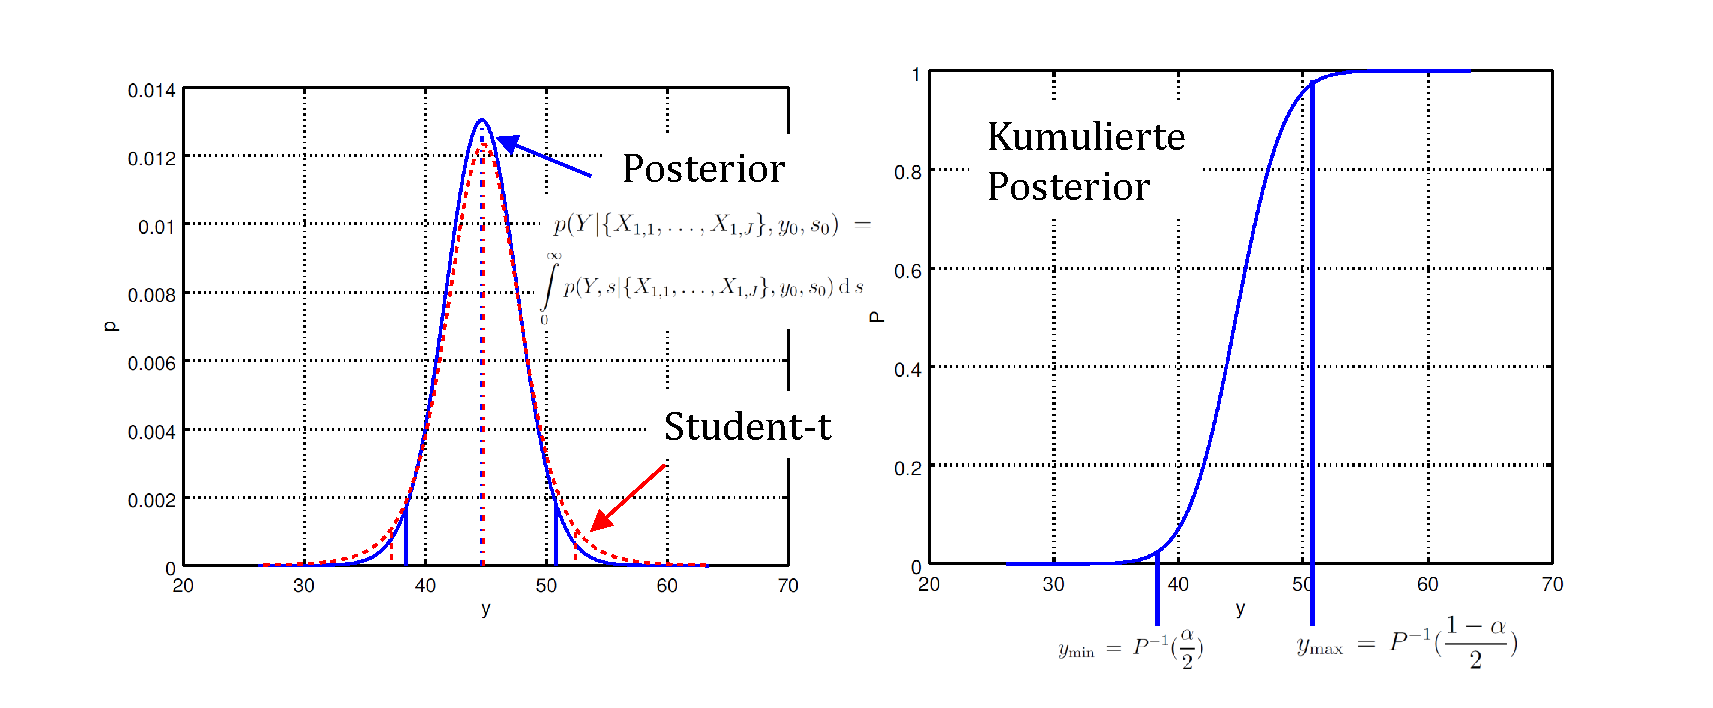
\includegraphics[width=160mm]{07_vorlesung/media/Ueberdeckungsintervall_0.pdf}
\caption{\label{VergleichsBeispiel}Wahrscheinlichkeitsdichtefunktionen und kumulierte Posterior
für die Bestimmung des Überdeckungsintervalls einer indirekten Messgröße}
\end{center}
\end{figure}
Wir berechnen für $\rho_{\mathrm{M}, \mathrm{K}} = 0$
$$
u^2(Y) \; = \;
\left(\frac{\partial}{\partial X_\mathrm{M}} X_\mathrm{M} X_\mathrm{K}
\right)^2_{\bar x_\mathrm{M}, K_0} \, s_\mathrm{M}^2 \; + \;
\left(\frac{\partial}{\partial X_\mathrm{K}} X_\mathrm{M} X_\mathrm{K}
\right)^2_{\bar x_\mathrm{M}, K_0} \, s_\mathrm{K}^2
$$
d.h.
$$
u(Y) \; = \;
\sqrt{ K_0^2 \, s_\mathrm{M}^2 \; + \; \bar x_\mathrm{M}^2 \, s_\mathrm{K}^2 }
\; = \; 4.802 \, \mathrm{E} .
$$
Die Anzahl der Freiheitsgrade berechnen wir gemäß der Satterthwaite'schen Gleichung
(\ref{EffectiveDFviele}), also
$$
\frac{u(Y)^4}{\nu_y} \; = \; \frac{K_0^4 \, s_\mathrm{M}^4}{\nu_\mathrm{M}} \; + \;
\frac{\bar x_\mathrm{M}^4 \, s_\mathrm{K}^4}{\nu_\mathrm{K}}
$$
d.h.\ mit $\nu_\mathrm{K} = 45$, $\nu_\mathrm{M} = 8$ und mit
$K_0 = 0.0925 \, \frac{\mathrm{E}}{\mathrm{V}}$, $s_\mathrm{K}=0.009 \, \frac{\mathrm{E}}{\mathrm{V}}$,
$\bar x_\mathrm{M} = 500.83 \, \mathrm{V}$, $s_\mathrm{M} = 17.89 \, \mathrm{V}$
$$
\nu_y \; = \; u(Y)^4 \, \left( \frac{K_0^4 \, s_\mathrm{M}^4}{\nu_\mathrm{M}} \; + \;
\frac{\bar x_\mathrm{M}^4 \, s_\mathrm{K}^4}{\nu_\mathrm{K}} \right)^{-1} \; = \;
52.58 \; \approx \; 52
$$
Die Anzahl der Freiheitsgrade kann auf ganzzahlige Werte abgerundet werden, das heißt die Nachkommastellen
 unterdrückt werden, siehe GUM JCGM 100:2008, Seite 73:
\begin{quote}
NOTE 1 If the value of $\nu_\mathrm{eff}$ obtained from Equation (G.2b) is not an integer,
which will usually be the case in practice, the corresponding value of $t_\mathrm{p}$ may be found
from Table G.2 by interpolation or by truncating $\nu_\mathrm{eff}$ to the next lower integer.
\end{quote}
\begin{lstlisting}[style=Matlab]
>> tinv(0.975,52)
ans =  2.0066
>> tinv(0.975,52.58)
ans =  2.0061
\end{lstlisting}
Wir verwenden für das t-Quantil (den Erweiterungsfaktor) den Wert $k = 2.006$, in der Praxis
nimmt man dann auch einfach $k = 2$.
Gemäß GUM kann die Formel für die effektive Anzahl von Freiheitsgraden also auch wie folgt
geschrieben werden
\begin{equation}
\nu_y \; = \;  \lfloor u(Y)^4 \, \left( \sum\limits_{i=1}^N \, \frac{ (c_i \, s_i)^4}{\nu_i}  \right)^{-1} \rfloor
\label{SatterthwaiteFloor}
\end{equation}
wobei die beiden Symbole $\lfloor r \rfloor$ um die Variable $r$ geschrieben heißen, dass
die Nachkommastellen von $r$ abzuschneiden sind, was in vielen Programmiersprachen mit der
Funktion \texttt{floor} erfolgt.

Das Vertrauensintervall wird damit schließlich
$$
[36.691 \, \mathrm{E}, 55.962 \, \mathrm{E}]
$$
und das vollständige Messergebnis
$$
Y \; = \; (46.327 \pm 9.635) \, \mathrm{E} .
$$
Der Wert für die erweiterte Unsicherheit $U = 9.635 \, \mathrm{E}$ entspricht also in etwa
dem Mittelwert aus den Berechnungen aus dem bayesischen Ansatz $\frac{1}{2} (9.423 + 9.907) =  9.665$.
Abb.~\ref{VergleichsBeispiel} zeigt das Prinzip anhand eines ähnlichen Beispiels, die eingezeichneten Werte
liegen weiter auseinander, um die Intervalle besser einzeichnen zu können.

%Bevor sich die Methoden der Kolmogoroffschen Wahrscheinlichkeitsrechnung, gemeinsame Verteilungen (\textsl{joined
%probability density distributions}) und entsprechende Margnalverteilungen zu berechnen, in der Metrologie
%(JCGM-Dokumente 101 und 102) durchgesetzt hatten, teils auch wegen der höheren Anforderungen an die Rechenleistung,
%hat man sich damit beholfen, in die Unsicherheitsfortpflanzung gemäß Gl.~(\ref{UnsicherFortpflLinearisiert}) anstelle
%von Varianzen normalverteilter oder $t$-verteilter Größen für einzelne Summanden auch

%Zu dem Kalibrierfaktor hatten wir die Anzahl der Freiheitsgrade als Information vorliegen.
%Oftmals liegen {\`a}-priori Informationen zu direkten Größen vor, ohne dass die Anzahl der
%Freiheitsgrade bekannt ist und auch ohne dass genauere Informationen zur Art der Verteilung vorliegen.
%Wie wir in der letzten Vorlesung schon gelernt haben, wird in einigen Fällen angenommen, dass
%die Verteilung sogar eine Rechteckverteilung ist, das heißt dass die Werte gleichverteilt über ein
%Intervall sind. Wir haben in dem Zusammenhang den Begriff der \textbf{Ermittlungsmethode Typ B der Messunsicherheit}
%eingeführt.

Für Größen, deren Messunsicherheit nicht unmittelbar aus vorliegenden
Stichproben gewonnen wurde, so dass Stichprobenumfang und Verteilungen nicht ermittelt
werden können, wird auf Basis heuristischer Vorstellungen eine Abschätzung der Anzahl der Freiheitsgrade
vorgenommen.

In Fällen, bei denen es um Präzisionsmessungen geht, kann vielfach angenommen werden,
dass die Anzahl der Freiheitsgrade gegen unendlich konvergiert.
\begin{equation}
\lim\limits_{\nu_i \rightarrow \infty} \, \left\{ \frac{ (c_i \, s_i)^4}{\nu_i} \right\} \; = \; 0
\end{equation}
Dies ist in Anhang G, Absatz G.4.3 des GUM JCGM 100:2008 nachzulesen. Lässt sich nicht
voraussetzen, dass die Anzahl der Freiheitsgrade sehr, sehr groß ist, so wird diese
abgeschätzt. Wie bei der Satterthwaite-Gleichung selbst, wird auch hier die Varianz der Varianz
%, siehe Anhang E, Absatz E.4.2
%\begin{equation}
%\operatorname{Var}(\bar s_i) \; \approx \; \frac{1}{2 \nu} \bar \sigma_i^2 ,
%\end{equation}
%wobei $\bar s_i$ die \textbf{empirische} Standardabweichung des Mittelwertes einer Größe $X_i$
%ist und $\bar \sigma_i = Var(X_i)$ die Standardabweichung dieser Größe ist, GUM Gl (E.7).
%Die Herleitung dieses Zusammenhangs ergibt sich aus der $\chi^2$-Verteilung, siehe Vorlesung 4 vom
%13.~November, Gln (33) bis (38) und 5.~Anhang \glqq Erwartungswerte zur $\chi^2$-Verteilung\grqq :
%$\operatorname{Var}(Q) = 2 \nu$ mit
%$Q = \nu \left(\frac{s}{\sigma}\right)^2$, so dass für die Standardabweichung der Einzelwerte gilt
\begin{equation}
\nu \; \sim \; \frac{\sigma_i^2}{\operatorname{Var}(s_i)}
\label{DFvsVariance}
\end{equation}
betrachtet, siehe GUM Anhang G, Absatz G.4.2.
Die Zuverlässigkeit der als {\`a}-priori Information mitgeteilten Unsicherheit muss
abgeschätzt werden mit einem bestimmten Prozentsatz
$(1 - \alpha) \cdot 100 \, \%$. Daraus wird heuristisch in Anlehnung an den
Zusammenhang (\ref{DFvsVariance}) die Anzahl der Freiheitsgrade abgeschätzt mit
\begin{equation}
\nu \; \approx \; \frac{1}{2 \alpha^2} .
\end{equation}
Der Quotient $\alpha$ wird als relative Unsicherheit $\frac{\Delta u}{u}$ der Unsicherheit $u$
interpretiert.

Nachdem wir gesehen haben, wie handlich die Berechnungen mit der klassischen Fortpflanzung
gegenüber den Methoden mit den Wahrscheinlichkeitsdichteverteilungen ist,
fragt man sich natürlich, weshalb wir den numerischen Aufwand mit dem Berechnen der
Integrale der Wahrscheinlichkeitsdichteverteilungen betreiben.
Für dieses kleine, handliche und anschauliche Beispiel ist dies selbstverständlich nicht
gerechtfertigt. Es dient lediglich dazu, das Grundprinzip des Verfahrens zu verdeutlichen.

Bei den Aufgaben, für die die Voraussetzungen zur Berechnung der Unsicherheit einer
indirekten Messgröße gemäß Gl.~(\ref{UnsichFortpfl2}) nicht mehr gegeben sind, werden die
Verfahren mit Rechnen mit Wahrscheinlichkeitsdichteverteilungen eingesetzt.
Dies sind Verfahren die entweder auf der Multiplikation von Likelihoodverteilungen - letztlich
auf Monte-Carlo-Berechnungen gemäß dem JCGM 101-Dokument der GUM-Reihe - oder auf der
bayesischen Statistik basieren.
Die Multiplikation von Likelihoodverteilungen setzt im Gegensatz zur bayesischen Statistik eine
\textsl{scharfe} \glqq Verteilung\grqq ~für die Modellfunktion ein. Dabei wird hier mit dem Begriff
\textsl{scharfe} Verteilung eine Wahrscheinlichkeitsdichte bezeichnet, die als Normalverteilung
mit dem Grenzübergang für $\sigma_\mathrm{winzig} \rightarrow 0$ in eine dirac'sche Deltafunktion übergeht.
Den Begriff \glqq Verteilung\grqq ~setzen wir hier in Anführungsstriche, weil
so eine dirac'sche Deltafunktion der Grenzfall ist, bei dem die Verteilung keine Verteilung mehr ist,
weil die Werte scharf und nicht mehr verteilt sind.

Bei dem Beispiel (mit Gun-Octave/matalb-Skript in Anhang \ref{AnhangBayesBeispiel})
haben wir die numerischen Integrationen in
sehr schlichter Weise dadurch realisiert, dass wir die betreffenden Größen in ein Raster äquidistanter
Stützstellen diskretisiert haben und dann einfach summiert haben. Es sollte hiermit nur das Grundprinzip der
Verfahren der \textsl{kolmogoroff'schen Wahrscheinlichkeitsrechnung} aufzeigen, die auch die Basis für die
Methoden der \textsl{bayesischen Statistik} bildet.

In vielen Fällen ist es aber nicht angesagt, beim numerischen Integrieren so zu verfahren.
Das nächste Kapitel soll deshalb einen kurzen
Überblick über unterschiedliche Verfahren zur numerischen Integration liefern.


\section{Aufgabe zum Selbststudium}
\label{AufgVor7}
Es sollen Abstände auf einem Werkstück mit Hilfe eines induktiven Wegaufnehmers gemessen werden.
Das Messprinzip eines induktiven Wegaufnehmers beruht darauf, dass
eine Wechselspannung ein Spulensystem im Sensor anregt.
Ein bewegliches ferro-magnetisches Teil am Sensor
beeinflusst die Induktivität in den Spulen.
Diese - in den Spulenteilen unterschiedliche - Induktivitätsveränderung wird vom
Messverstärker ausgewertet und in ein positions-proportionales Gleichspannungssignal
umgewandelt.

Um die Abstände in der physikalischen Einheit Mikrometer zu erhalten, muss mit Hilfe
eines Bezugsnormals aus dem Spannungssignal ein Weg mit der Dimension einer Länge
berechnet werden.
Es ist bekannt, dass in dem für die Messung relevanten Messbereich (Hub des Sensors)
die Abhängigkeit zwischen Spannungssignal und Auslenkung des ferro-magnetischen Kerns
linear ist.
Das Bezugsnormal ist eine Stufenhöhe.

Zu dem Bezugsnormal gibt es einen Kalibrierschein, der folgenden Höhenwert für das
Normal angibt:
\begin{equation}
d \; = \; (4.997 \pm 0.011) \; \mathrm{\mu m} \qquad \mathrm{mit} \qquad k = 2.1, \nu = 26
\label{kalBezug}
\end{equation}

Mit dem induktiven Wegaufnehmer wurden auf dem Bezugsnormal folgende Stufenhöhen in
der Dimension der elektrischen Spannung mit der Einheit Millivolt gemessen

% muB = 200; sigB = 8;
% JB = 11; xB = muB+sigB*randn(1,JB);
% printf("& %4.1f ", xB);
% xB = [201.3  187.3  196.5  200.4  193.6  174.2  197.2  185.4  194.4  202.5  205.2];
Tabelle A5.1:\\
\begin{tabular}{c||c|c|c|c|c|c|c|c|c|c|c}
\hline
$U_\mathrm{B} / \mathrm{mV}$ & 201.3 & 187.3 & 196.5 & 200.4 & 193.6 & 174.2 & 197.2 & 185.4 & 194.4 & 202.5 & 205.2\\
\hline
\end{tabular}

%Für den Abstand auf dem Werkstück wurden folgende Spannungen gemessen
%>> muW = 180; sigW = 11;
%>> JW = 7; xW = muW+sigW*randn(JW,1);
%>> printf(" %4.1f ", xW);
% 176.5  184.1  180.5  193.6  176.0  194.5  160.9 >>
%>> printf("& %4.1f ", xW);
Tabelle A5.2:\\
\begin{tabular}{c||c|c|c|c|c|c|c}
\hline
$U_\mathrm{W} / \mathrm{mV}$ & 176.5 & 184.1 & 180.5 & 193.6 & 176.0 & 194.5 & 160.9 \\
\hline
\end{tabular}

Der Zusammenhang zwischen dem Abstand auf dem Werkstück in Mikrometern $d_\mathrm{W}$,
der Stufenhöhe des Bezugsnormals gemäß Kalibrierschein $d$, dem gemessenen Spannungssignal
an der Stufenhöhe $U_\mathrm{B}$ und dem gemessenen Spannungssignal $U_\mathrm{W}$ am Werkstück
ist folgender
\begin{equation}
d_\mathrm{W} \; = \; \frac{d}{U_\mathrm{B}} \, U_\mathrm{W}
\end{equation}

Die Änderungen aufgrund der statistischen Streuung der Spannungswerte $U_\mathrm{B}$ sind
so klein, dass für die Sensitivität $c_\mathrm{B}$ von $d_\mathrm{W}$
bezüglich Änderungen von $U_\mathrm{B}$
mit dem hyperbolischen Zusammenhang $d_\mathrm{W} \sim \frac{1}{U_\mathrm{B}}$
die Steigung der Tangenten an die Hyperbel verwendet wird. Es wird die
Tangente verwendet, die an dem Punkt, der sich aus den Mittelwerten
ergibt, anliegt.
\begin{equation}
c_\mathrm{B} \; = \; \left. \frac{\partial}{\partial U_\mathrm{B}}
 d_\mathrm{W} \right|_{\bar U_\mathrm{B}, \bar d, \bar U_\mathrm{W}}
\end{equation}
Die Sensitivitäten $c_\mathrm{d}$ und $c_\mathrm{W}$ von $d_\mathrm{W}$
bezüglich Änderungen von $d$ und $U_\mathrm{W}$ sind aufgrund des
linearen Zusammenhangs genau
\begin{equation}
c_\mathrm{d} \; = \; \left. \frac{U_\mathrm{W}}{U_\mathrm{B}} \right|_{\bar U_\mathrm{B}, \bar U_\mathrm{W}} \qquad
c_\mathrm{W} \; = \; \left. \frac{d}{U_\mathrm{B}} \right|_{\bar U_\mathrm{B}, \bar d}
\end{equation}
definiert.
Die kombinierte Varianz unter der Voraussetzung, dass die gemessenen Größen und
die Angabe aus dem Kalbrierschein unkorreliert sind, ist
\begin{equation}
s_\mathrm{dW}^2 \; = \; (c_\mathrm{d} \, s_\mathrm{d})^2 \; + \;
(c_\mathrm{B} \, s_\mathrm{B})^2 \; + \; (c_\mathrm{W} \, s_\mathrm{W})^2
\end{equation}
mit $s_\mathrm{B}$ für die Standardabweichung der in Tabelle A5.1 aufgelisteten Werte,
$s_\mathrm{W}$ für die Standardabweichung der in Tabelle A5.2 aufgelisteten Werte und
$s_\mathrm{d}$ für die Standardabweichung der Angabe aus dem Kalibrierschein.

\begin{itemize}
\item[a)] Ermitteln Sie aus den Angaben des Kalibrierscheins (hier Gl.~(\ref{kalBezug}))
die Standardabweichung $s_\mathrm{d}$, indem Sie den dort genannten Erweiterungsfaktor verwenden.
%>> d = 4.997 d =  4.9970
%>> sd = 0.011/2.1 sd =  0.0052381
\item[b)] Ermitteln Sie die beiden Mittelwerte $\bar U_\mathrm{B}$ und $\bar U_\mathrm{W}$,
sowie die beiden empirirschen Standardabweichungen $s_\mathrm{B}$ und $s_\mathrm{W}$
aus den beiden Tabellen A5.1 und A5.2.
%>> xBbar = mean(xB) xBbar =  194.36
%>> xWbar = mean(xW) xWbar =  180.85
%>> sW = std(xW) sW =  11.561
%>> sW2 = var(xW) sW2 =  133.65
%>> sB = std(xB) sB =  9.0410
%>> sB2 = var(xB) sB2 =  81.739
\item[c)] Bestimmen  Sie die Sensitivitäten $c_\mathrm{d}$, $c_\mathrm{W}$, $c_\mathrm{B}$ durch Ausführen der
partiellen Ableitung.
%(%i4) dW(UB) := UW*d/UB;
%                                          UW d
%(%o4)                           dW(UB) := ----
%                                           UB
%(%i5) diff(dW(UB),UB);
%                                      d UW
%(%o5)                               - ----
%                                        2
%                                      UB
\item[d)] Berechnen Sie die kombinierte empirische Standardabweichung $s_\mathrm{dW}$.
%>> cd = xWbar/xBbar cd =  0.93048
%>> cW = d/xBbar cW =  0.025710
%>> cB = -d*xWbar/(xBbar^2) cB = -0.023922
%s2 = (sd*cd)^2 + sW2*cW^2 + sB2*cB^2 s2 =  0.13514
%s = sqrt((sd*cd)^2 + sW2*cW^2 + sB2*cB^2) s =  0.36762
\item[e)] Berechnen Sie die effektive Anzahl der Freiheitsgrade.
%nueff = s2^2 / ((sd*cd)^4/26 + (sW2*cW^2)^2/(JW-1) + (sB2*cB^2)^2/(JB-1)) nueff =  12.019
\item[f)] Berechnen Sie den Erweiterungsfaktor $k$, der
 hier das t-Quantil für ein zweiseitiges Vertrauensniveau
 von $1-\alpha = 0.95\%$ ist.
% k=tinv(0.975,nueff) k =  2.1784
\item[g)] Bestimmen Sie das vollständige Messergebnis.
% dW = d*xWbar/xBbar  dW =  4.6496
% k*s =  0.80083
% d_W = 4.6496 \pm 0.80083
\end{itemize}

\newpage

\section{Anhang: Erwartungswerte zur $\chi^2$-Verteilung}
\label{ErwaChi2}
Die $\chi^2$-Verteilung ist definiert durch
% p(Q,nu):= (Q^((nu/2)-1)) * exp(-Q/2) / (gamma(nu/2) * 2^(nu/2));
\begin{equation}
p(Q,\nu) \; := \; \frac{ Q^{\frac{\nu}{2}-1} \; e^{-\frac{Q}{2}}}
{\Gamma\left(\frac{\nu}{2}\right) \; 2^{\frac{\nu}{2}}} \qquad \nu \in I \! \! N
\end{equation}
mit
% gamma(nu/2) = sqrt(pi) *((nu-2)!!) / 2^((nu-1)/2)
\begin{equation}
\Gamma\left(\frac{\nu}{2}\right) \; = \; \sqrt{\pi} \, \frac{(\nu-2)!!}{2^{\frac{\nu-1}{2}}}
\end{equation}
und
\begin{equation}
\nu!! = \nu (\nu-2) (\nu-4) ... 4 \cdot 2 .
\end{equation}
Der Erwartungswert für die Zufallsgröße $Q$ ist
\begin{equation}
\operatorname{E}(Q) \; = \; \int\limits_{0}^{\infty} \, Q^\prime \, p(Q^\prime,\nu) \,
\operatorname{d}Q^\prime
\end{equation}
und nach Integration mit Computeralgebrasoftware (beispielsweise Maxima)
%                                        nu
%                                2 gamma(-- + 1)
%                                        2
%(%o6)                           ---------------
%                                         nu
%                                   gamma(--)
%                                         2
\begin{equation}
\operatorname{E}(Q) \; = \; \frac{2 \Gamma\left(\frac{\nu}{2} + 1 \right)}{\Gamma\left(\frac{\nu}{2}\right)}
\end{equation}
und mit
$$
\Gamma\left(\frac{\nu}{2} + 1 \right) =
\Gamma\left(\frac{\nu}{2} + \frac{2}{2} \right) = \Gamma\left(\frac{\nu+2}{2}\right)
$$
und
$$
\Gamma\left(\frac{\nu+2}{2}\right) = \sqrt(\pi) \, \frac{(\nu+2-2)!!}{2^{(\nu+2-1)/2}}
$$
erhalten wir
\begin{equation}
\arraycolsep=2.4pt\def\arraystretch{2}
\begin{array}{ll}
2 \frac{\Gamma(\nu/2 + 1)}{\Gamma(\nu/2)}
 & = 2 \frac{(\nu)!!}{(\nu-2)!!} \; \frac{ 2^{(\nu-1)/2} }{ 2^{(\nu-1)/2 + 1}}\\
 & = 2 \frac{(\nu)!!}{(\nu-2)!!} \; \frac{1}{2} \\
 & = \nu
\end{array}
\end{equation}
Der Erwartungswert für die Varianz $\operatorname{Var}(Q)$ von $Q$ ist
\begin{equation}
\operatorname{Var}(Q) \; = \; \int\limits_{0}^{\infty} \, (Q^\prime
- \nu)^2 \, p(Q^\prime,\nu) \,
\operatorname{d}Q^\prime
\end{equation}
und nach Integration mit dem Computeralgebraprogramm Maxima
\begin{equation}
\operatorname{Var}(Q) \; = \; \nu^2 \; - \;
2 \nu \frac{\Gamma(\nu/2 + 1)}{\Gamma(\nu/2)} \; + \;
2 \frac{\Gamma(\nu/2 + 2)}{\Gamma(\nu/2)}
\end{equation}
%       2  nu/2       nu        nu/2 + 2       2 + nu     nu/2 + 2       4 + nu
%     nu  2     gamma(--) - nu 2         gamma(------) + 2         gamma(------)
%                     2                          2                         2
%     --------------------------------------------------------------------------
%                                   nu/2       nu
%                                  2     gamma(--)
%                                              2
%(%i9) = nu^2 - 2*nu^2 + nu*(nu+2) = 2*nu
d.h.
\begin{equation}
\operatorname{Var}(Q) \; = \; \nu^2 \; - \; 2 \nu^2 \; + \; \nu (\nu+2) \; = \; 2 \nu
\end{equation}

\newpage

\section{Anhang: Beispiel indirekte Größe aus Produkt zweier direkter Größen}
\label{AnhangBayesBeispiel}
Gnu-Octave Code zu dem Beispiel aus Abschnitt~\ref{MUFklassischvsbayes}

%\lstset{language=Matlab}
\lstinputlisting[style=Matlab]{07_vorlesung/code/bayes_indirect_quantity_product.m}

%
\chapter{Numerische Werkzeuge für Messunsicherheitsberechnungen}

\section{Numerische Integrationsverfahren}
Sei $p$ eine Funktion $p \! : Y \rightarrow p(Y)$, die numerisch über ein
Intervall $[y_1, y_2]$ integriert werden soll.
\begin{equation}
P(y_1, y_2) \; = \; \int\limits_{y_1}^{y_2} \, p(Y) \, \operatorname{d}Y
\end{equation}
Integrieren bedeutet, die Fläche unter der Kurve zu berechnen. Wir approximieren die
Fläche unter der Kurve durch Rechtecke einer festen Breite $\Delta Y$ und einer Höhe
$p(Y_i)$ in der in Abb.~\ref{Trapez} dargestellten Weise.
\begin{figure}
\begin{center}
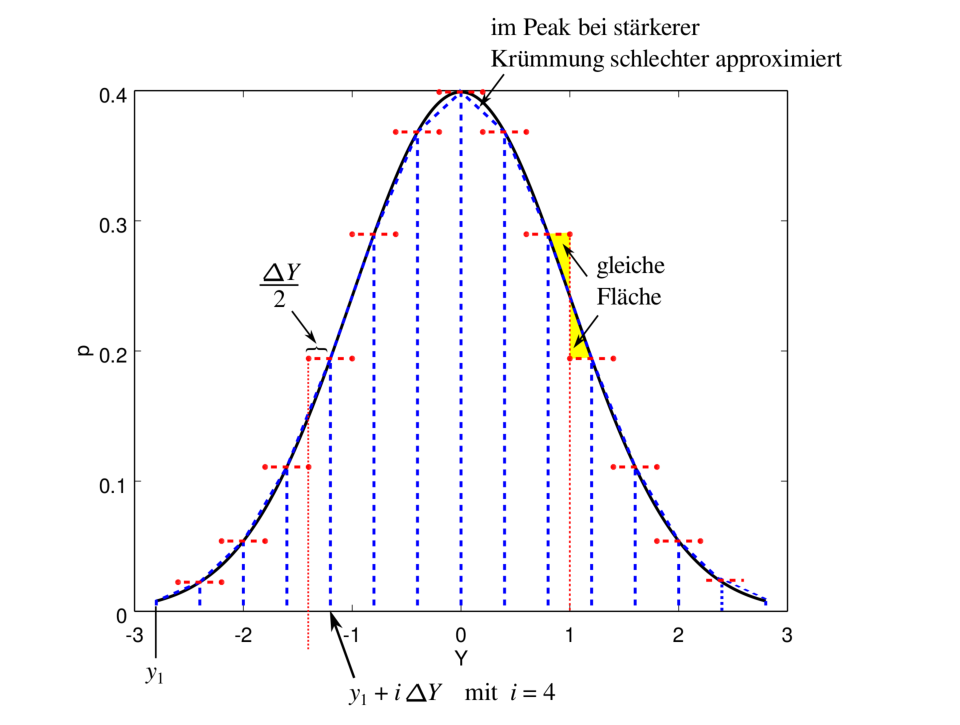
\includegraphics[width=130mm]{07_vorlesung/media/numerischeIntTrapez.pdf}
\caption{\label{Trapez} Trapezapproximation für die Berechnung der Fläche unter einer
Kurve zur numerischen Integration.}
\end{center}
\end{figure}
Die Flächen der mit rot, gestrichpunkteter Linie gekennzeichneten Rechtecke sind genauso
groß wie die mit blau gestrichelter Umrandung markierten Trapezstücke. Diese Flächen
werden summiert, um näherungsweise die Fläche unter der Kurve zu bestimmen.
Das erste und das letzte Flächenstückchen sind nur halb so groß.
Das Integrationsintervall wird in $n$ Flächen unterteilt, so dass für die Breite
der Flächenstücke gelte
\begin{equation}
\Delta Y \; = \; \frac{y_2 - y_1}{n} .
\end{equation}
Es wird nun so aufgeteilt, dass $n-1$ Stücke betrachtet werden gemäß den rot
gestrichpunkteten Rechtecken mit der Breite $\Delta Y$ und zwei weitere Stücken je
der Hälfte dieser Breite und je eines ganz am Anfang und das andere als letztes
Stückchen ganz am Ende.
Das erste Stückchen hat die halbe Breite und die Fläche
$$
\underbrace{\frac{\Delta Y}{2} \, p(y_1)}_{\mathrm{Rechteck}}
 \; + \;
\underbrace{\frac{\Delta Y}{4} \, (p(y_1 + \frac{\Delta Y}{2}) - p(y_1))}_{\mathrm{Dreieck}}
\; = \;
\frac{\Delta Y}{4} \, (p(y_1 + \frac{\Delta Y}{2}) + p(y_1))
$$
das letzte Stückchen analog
$$
\frac{\Delta Y}{4} \, (p(y_2 - \frac{\Delta Y}{2}) + p(y_2))
$$
so dass für die gesamte Fläche gilt
\begin{equation}
P(y_1, y_2) \; = \; \varepsilon \; + \;
\frac{\Delta Y}{4} \, \left(p(y_1 + \frac{\Delta Y}{2}) + p(y_1) +
p(y_2 - \frac{\Delta Y}{2}) + p(y_2)\right) \; + \;
\sum\limits_{i=1}^{n-1} \,
p(y_1 \, + \, i \, \Delta Y) \, \Delta Y
\end{equation}
mit $\varepsilon$ für die Abweichung von der Fläche, die unter der Kurve liegt.
Dabei gilt es eine geeignete Wahl für die Breite $\Delta Y$ der Intervalle
oder andersrum ausgedrückt für die Anzahl $n$ der Intervalle zu treffen.

Eine Möglichkeit ist, sich iterativ zu einer sinnvollen Anzahl von Intervallen
vorzuarbeiten, indem die Intervallbreite $\Delta Y$ mit jedem Iterationsschritt halbiert wird.
Dabei arbeitet man sich solange vor bis sich die approximierte Fläche
durch weiteres Halbieren der Intervallbreiten nicht mehr
signifikant ändert. Diese Methode wird \textsl{Romberg}-Verfahren genannt.
Werner Romberg war ein in Berlin geborener Mathematiker, der in Heidelberg und München
studierte und promovierte. Kurz nach dem Rigorosum im Jahr 1933 musste er als Kritiker
des Nazionalsozialismus Deutschland verlassen. 1949 wurde Werner Romberg Dozent für Physik
am Norwegian Institute of Technology (NTH) in Trondheim und richtete dort den Studiengang
für Mathematische Physik ein. 1955 publizierte er dieses numerische Integrationsverfahren.

Ein Quellcode-Beispiel in C ist auf der Wikipediaseite zum Romberg-Verfahren zu finden:
\begin{verbatim}
https://en.wikipedia.org/wiki/Romberg%27s_method
\end{verbatim}
Bei jedem Iterationsschritt wird $\Delta Y$ halbiert.
Der Iterationsschritt $n = 1$ bedeutet $\Delta Y_1 = y_2 - y_1$, Schritt $n = 2$
bedeutet $\Delta Y_2 = (y_2 - y_1)/2 = \Delta Y_1/2$ etc.
\begin{equation}
P_n (y_1, y_2) \; = \;
\frac{\Delta Y_n}{4} \, (p(y_1 + \frac{\Delta Y_n}{2}) + p(y_1) +
p(y_2 - \frac{\Delta Y_n}{2}) + p(y_2)) \; + \;
\sum\limits_{i=1}^{n-1} \,
p(y_1 \, + \, i \, \Delta Y_n) \, \Delta Y_n
\end{equation}
mit
$$
 \Delta Y_n \, = \, \frac{1}{2} \Delta Y_{n-1} .
$$
Die Iteration endet, sobald der Betrag der Differenz der approximierten Flächen
\begin{equation}
\mid P_n (y_1, y_2) \, - \, P_{n-1} (y_1, y_2) \mid \, < \, \varepsilon_P
\end{equation}
einen Wert annimmt, der kleiner als ein zuvor definierter sehr kleiner Wert $\varepsilon_P$ ist.

Dabei werden die Flächenstücke durch Halbierung der Intervallbreite gleichförmig schmaler gemacht.
Die einzelnen Abweichungen zu jedem der Intervalle können für unterschiedlich stark gekrümmte
Segmente der unterschiedlichen Stückchen verschieden groß sein, so dass für manche
Anwendungen dadurch Rechenzeit gesparen werden, dass nur ausgewählte Bereiche
verfeinert werden. Hier ist mehr Aufwand bei der Implementierung der Verästelung des Baumes,
der für unterschiedlichen Integrationsbereiche unterschiedliche Iterationstiefen verwaltet,
erforderlich. Wir nennen die Grenzen der Flächenstückchen, die bei Romberg gleichförmig die Positionen
$$
Y_i \, = \, y_1 \, + \, (i-1) \Delta Y
$$
annehmen, \textsl{Samples}, für die im allgemeinen gelten kann
\begin{equation}
Y_{i+1} - Y_i \, \neq \, Y_{k+1} - Y_k \quad \mathrm{f{"u}r} \quad i \neq k .
\end{equation}

%Ein Maß dafür, um wieviel die trapezförmigen Flächenstücke zu
%groß oder zu klein sind, ist beispielsweise der Abstand $\delta_i$
%zwischen der jeweiligen Sekante und dem Wert
%der Funktion $p$ in der Mitte der Sekante (blau gestrichelte Linien)
%\begin{equation}
%\delta_i \; = \; p(y_1 \, + \, i \Delta Y \, - \, \frac{\Delta Y}{2}) \; -
%\; \frac{1}{2} \left( p(y_1 \, + \, i \Delta Y) +  p(y_1 \, + \, (i-1) \Delta Y ) \right) .
%\end{equation}
%Bei Funktionsverläufen mit relativ gleichförigem Krümmungsverhalten wird
%ein integrales Maß aus den $\delta_i$ verwendet, um zu bewerten ob sich bei feinerer

Insbesondere bei der Integration mehrdimensionaler Funktionen, wie wir sie
in unseren Bespielen hatten, bevor wir die Marginalverteilung erworben hatten,
also soetwas wie bei folgender Integration
$$
\int\limits_{-\infty}^\infty \cdots \int\limits_{-\infty}^\infty
p(Y, X_1, \dots, X_N | \{X_{i,1}, \dots, X_{i,J_i}\}, \bar x_k, s_k, \dots)
\operatorname{d}X_1 \dots \operatorname{d}X_N
$$
gilt es die \textsl{Samples} für die Hypervolumenstückchengrenzen optimal zu wählen.
Die Berechnungen sollen in minimaler Zeit fertig werden und dennoch soll das
gesamte Hypervolumen möglichst genau approximiert werden.

Betrachten wir konkret die Aufgabe, Wahrscheinlichkeitsdichteverteilungen $p$
integrieren zu wollen, welche dadurch gekennzeichnet sind, dass ihre Funktionswerte
positiv sind und dass sie aus einem
oder vielleicht auch ganz wenig mehr als einem breiteren \textsl{Peak} (Glocke) bestehen.
Diese Glocke muss dabei nicht unbedingt so schön symmetrisch sein wie bei der
Normalverteilung oder bei der Student-t-Verteilung, sondern kann eine gewisse Schiefe haben
wie beispielsweise bei der $\chi^2$-Verteilung für wenige Freiheitsgrade.
Wenn wir Abb.~\ref{Trapez} genauer anschauen, sehen wir, dass die Sekanten im Zentrum
des \textsl{Peaks}, der Glocke, stärker von der Kurve der Glocke abweichen als in den
\textsl{Tails}. Die Sample-Stützstellen wollen wir also im Bereich des Glockenmaximums, bzw.\
in den Bereichen der Glockenmaxima, enger legen als in den \textsl{Tails}. Dies ist äquivalent
zu dem, die Dichte der Stützstellen gemäß der Verteilung $p$ selbst zu samplen.
Mit anderen Worten, es wird eine nach $p$ verteilte Stichprobe der Größen $X_i$
entnommen. Die Verteilung $p$ wird verwendet, um gleichverteilte Pseudozufallszahlen auf nach $p$
verteilte Zahlen abzubilden.
Dieser Ansatz liegt den sogenannten \textsl{Importance Sampling}-Algorithmen zugrunde.

Wenn eine Verteilung $p$ stark fluktuiert, also innerhalb eines
Intervalls (des $i$-ten Intervalls) auf der $X$-Achse sehr unterschiedliche Funktionswerte $p(X_i)$ annimmt,
so bedeutet das, dass $p(X_i)$ eine große Varianz hat.
\begin{equation}
\operatorname{Var}(p(X_i)) \; = \; \frac{1}{J-1} \sum_{j=1}^J \, \left(p(X_{i,j})- \bar p(X_i)\right)^2 .
\end{equation}
Die Varianz bezüglich unterschiedlicher Intervalle, bzw.\ Regionen, wird als Maß verwendet,
das der Entscheidung zugrunde gelegt wird, ob weitere Stützstellen in dieser Region
gesampelt werden, die Region in kleinere Regionen zu unterteilen, um je Region kleinere Varianzen
zu erhalten.
Das Sampeln innerhalb der verschiedenen Regionen geschieht dabei
voneinander unabhängig. Die Regionen werden auch Gruppen oder Schichten genannt.
Ein nach diesem Verfahren gebildetes Sample heißt \textsl{geschichtete Zufallsstichprobe}
oder \textsl{stratifizierte Zufallsstichprobe} (engl.\ \textsl{stratified Sample}).

\section{Zufallszahlen und Wahrscheinlichkeitsverteilungen}
Die Thematik des Samplings nach Methoden, bei denen Zufallszahlen verwendet werden, ist ein
weites Feld in der Statistik. Große Bedeutung haben zufallszahlenbasierte Integrationsmethoden,
die auf Erkenntnissen aus der Thermodynamik, d.h.\ der statistischen Physik beruhen.
Sie wurden aus Beobachtung der brown'schen Molekularbewegung abgeleitet, also aus der
Zufälligkeit und Art und Weise der Bewegung von Molekülen eines Fluids.
Der zurückgelegte Pfad eines Moleküls, \textsl{Random Walk},
ändert zufällig die Richtung.
%, aber die Einzelpositionen haben eine gewisse Autokorrelation.

Die Abfolge der Transformationen, die eine aktuelle Position eines Gegenstands oder den
aktuellen Zustand eines Prozesses in die nachfolgende Position bzw.\ den nachfolgenden
Zustand überführt, und daraus die danach nachfolgende Position (den daraus folgenden Zustand)
und so weiter, heißt \textsl{Markow-Kette}. Kennzeichen einer Markow-Kette ist, dass die
Positions\-änder\-ung des Moleküls nur von der aktuellen Position,
nicht aber von den Positionen davor, abhängt. Allgemein lassen sich viele statistische Prozesse,
nicht nur Pfade von Fluidpartikeln oder Abfolgen der Werte von Zufallssampeln, mit Hilfe von
Markow-Ketten beschreiben und es gilt:
\begin{quote}
Der zukünftige Zustand des Prozesses ist nur durch den
aktuellen Zustand bedingt und wird nicht durch vergangene Zustände beeinflusst.
\end{quote}

Um rechentechnisch mit Zufallszahlen zu arbeiten, müssen diese synthetisch generiert werden.
Synthetisch gerechnete Zufallszahlen beruhen auf definierten Algorithmen und
sind deshalb nicht wirklich zufällig, sondern deterministisch. Sie werden deshalb
\textsl{Pseudozufallszahlen} genannt.
Ein deterministischer Algorithmus berechnet eine Zahlenfolge, die nur den
Anschein hat, dass die Zahlenwerte zufällig verteilt sind und nicht deterministisch.

Prinzipiell ist ein solcher Algorithmus, oftmals Zufallszahlengenerator genannt, wie
folgt aufgebaut.
\begin{enumerate}
\item Setzen eines Startwertes, der \textsl{Seed} genannt wird, was ein englischsprachiger
  Begriff ist und Saat, Samenkorn heißt.
\item Wechselweise Multiplikationen und Restklassenoperationen mit sehr großen natürlichen Zahlen, wobei
  bei der Restklassenoperation als Teiler eine möglichst große Primzahl, beispielsweise
  16807, zum Einsatz kommt.
\end{enumerate}
Mit Restklassenoperation ist hier gemeint, dass eine Division mit natürlichen Zahlen
durchgeführt wird, deren Rest als Ergebnis in die weiteren Berechnungsschritte eingeht.


\begin{figure}
\begin{center}
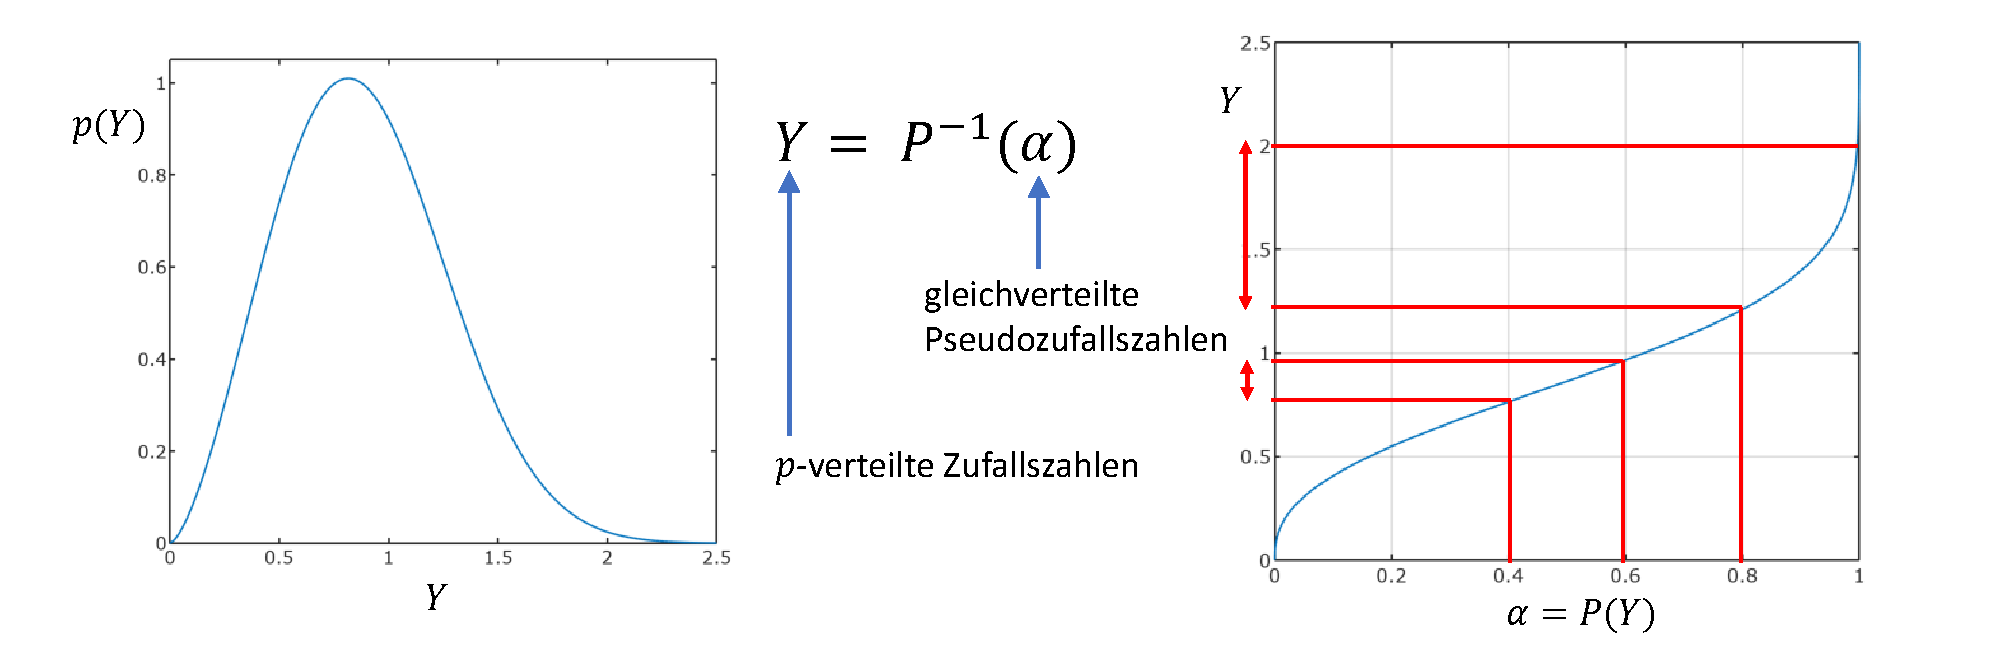
\includegraphics[width=160mm]{07_vorlesung/media/TransformRandomDistri.pdf}
\caption{\label{pverteilteZufallszahlen} Eine gleichverteilte Größe wie beispielsweise
eine Wahrscheinlichkeit $\alpha$ wird über die inverse Funktion $P^{-1}$ der
kummulierten Wahrscheinlichkeitsverteilung $P$, also der aufintegrierten Verteilung
der Wahrscheinlichkeitsdichte $p$, abgebildet auf die Größe $Y$, die dann $p$-verteilt ist.}
\end{center}
\end{figure}
Die heutigen Bibliotheken für Compiler und Programmiertools wie Matlab bieten nicht nur
Zufallszahlengeneratoren, die gleichverteilte Zahlenfolgen liefern. Sie stellen schon
fertige, schnelle, effektive Algorithmen zur Verfügung, die die Transformation auf die üblichen
Verteilungsdichtefunktionen $p$ zur Verfügung stellen. So ist \texttt{randn} der Name der Funktion
in Matlab und Gnu-Octave zur Erzeugung von normalverteilten Zufallszahlen. \texttt{rande}
liefert exponentiell verteilte Zufallszahlen, \texttt{randg} Zufallszahlen, die nach
der Gammafunktion verteilt sind und \texttt{randp} poissonverteilte Zufallszahlen. In Python sind
diese in der zu \texttt{numpy} gehörenden Biblothek \texttt{random} zu finden. Mit
\texttt{randn} werden standardnormalverteilte Zufallszahlen erzeugt:
%\lstset{language=Python}
\begin{lstlisting}[style=Python]
import numpy as np
nrow = 5
ncol = 20
a = np.random.randn(nrow, ncol)
\end{lstlisting}
Mit \texttt{rand} werden gleichverteilte Zufallszahlen $R \in [0, 1)$ erzeugt.

Wir können aber auch selber gleichverteilte Zufallszahlen abbilden auf eine andere Verteilung $p$,
wenn wir die Umkehrfunktion der kumulierten Verteilung $P^{-1}$ dazu zur Verfügung haben.
Sei $R = \{R_1, \dots, R_J\}$ ein Sample, eine Stichprobe, gleichverteilter Zufallszahlen mit
$R \in [0,1)$, so ist die Menge der mit $P^{-1}$ transformierten Zufallszahlen
$$
Z \; = \; P^{-1}(R)
$$
gemäß $p$ verteilt, siehe Abb.~\ref{ZufallszahlenAbbilden}.

Als Beispiel wollen wir in Python 1000 Zufalls\-zahlen generieren,
die verteilt sind gemäß einer $t$-Verteilung für 45 Freiheitsgrade:
%\lstset{language=Python}
\begin{lstlisting}[style=Python]
import numpy as np
import scipy
from scipy import stats
Jz = 1000
nu = 45
R = np.random.rand(1, Jz)
Z = scipy.stats.t.ppf(R[0], nu)
\end{lstlisting}

\section{Monte-Carlo-Verfahren gemäß GUM-supplement~1 JCGM 101}

In Kapitel~\ref{montecarloMU} werden wir das Monte-Carlo-Verfahren gemäß GUM-supplement~1 JCGM 101
erläutern, bei dem wie oben bereits erwähnt,
gemäß den jeweiligen Ver\-teil\-ungen der unterschiedlichen direkten Messgrößen
eine große Stichprobe (ein großes \textsl{Sample})
$\mathbf{x}_1 = (x_{1,1},\dots,x_{N,1})^\mathsf{T}$, $\dots$, $\mathbf{x}_J = (x_{1,J},\dots,x_{N,J})^\mathsf{T}$
für die direkten Größen $\mathbf{X}$ per Zufallszahlengenerator erzeugt
wird. Diese wird in das Modell $f$ gesteckt,
um eine Stichprobe
\begin{equation}
y_1 = f(x_{1,1},\dots,x_{N,1}), \dots, y_J = f(x_{1,J},\dots,x_{N,J})
\end{equation}
der indirekten Größe $Y$ zu gewinnen. Entweder wird aus der inversen Funktion der kumulierten
Wahrscheinlichkeitsverteilung das Überdeckungsintervall gewonnen oder es werden aus dem Sample $y_1,\dots, y_J$
der Erwartungswert $\bar y$ und die Standardabweichung $\sigma_Y$ gemäß
$$
\bar y = \frac{1}{J} \sum_{j=1}^{J} y_j \qquad
\sigma_Y = \sqrt{\frac{1}{J-1} \sum_{j=1}^{J} (y_j - \bar y)^2}
$$
berechnet.

Dieses Verfahren entspricht gemäß \cite{Wue08} in etwa den Berechnungen wie
in Gl.~(\ref{PosteriorSensor}), nämlich wenn wir für die Standardabweichung $\sigma_\mathrm{winzig}$
den Grenzübergang $\sigma_\mathrm{winzig} \rightarrow 0$ machen, sodass die zu integrierende
Verteilung in die folgende übergeht:
\begin{equation}
\arraycolsep=2.0pt\def\arraystretch{2.0}
\begin{array}{l}
p(Y, X_\mathrm{K}, X_\mathrm{M} | (X_{\mathrm{M},1}, \dots, X_{\mathrm{M},J}), K_0, s_\mathrm{K}) \propto \\
\delta\left(Y \; - \; X_\mathrm{K} \, X_\mathrm{M}\right)
\;  e^{-\frac{1}{2} \left(\frac{X_\mathrm{K} - K_0}{s_\mathrm{K}} \right)^2} \; \prod\limits_{j=1}^J  \,
e^{-\frac{1}{2} \left(\frac{ X_\mathrm{M} - X_{\mathrm{M},j} }{s_\mathrm{M}} \right)^2}
\end{array}
\label{PosteriorFall4}
\end{equation}
Zu den Größen $X_\mathrm{K}$ und $X_\mathrm{M}$ werden dann zufällige
Samples gewählt.

Im folgenden werden wir den Grenzübergang der Wahrscheinlichkeitsdichte für das Modell
\begin{equation}
\lim_{\sigma \rightarrow 0} \left\{ e^{-\frac{1}{2} \left(\frac{Y-f(\mathbf{X})}{\sigma}\right)^2} \right\}
= \delta\left(Y \; - \;f(\mathbf{X})\right)
\end{equation}
in eine dirac'sche Distribution als \textsl{scharfen Modellprior} bezeichnen.

Für univariate, explizite Modellfunktionen und für normalverteilte Größen $X_i$ sieht die
Posterior mit \textsl{scharfem Modellprior} dann wie folgt aus
\begin{equation}
\arraycolsep=2.0pt\def\arraystretch{2.0}
\begin{array}{l}
p(Y, X_\mathrm{1}, \dots, X_\mathrm{N} | (X_{1,1}, \dots, X_{1,J_1}), ..., (X_{K,1}, \dots, X_{K,J_1}),
 \bar x_{K+1}, s_\mathrm{K+1}, \dots, \bar x_{N}, s_\mathrm{N}) \propto \\
\delta\left(Y \; - \; f(X_1, \dots \, X_N)\right)
\; \left( \prod\limits_{i=1}^K \, \prod\limits_{j=1}^{J_i}  \,
e^{-\frac{1}{2} \left(\frac{ X_i - X_{i,j} }{s_i} \right)^2} \right)
\;  \left( \prod\limits_{i=K+1}^N \,  e^{-\frac{1}{2} \left(\frac{X_i - \bar x_i}{s_i} \right)^2} \right) .
\end{array}
\label{PosteriorFall4allgemeiner}
\end{equation}


Wir hatten bereits angesprochen, dass die Monte-Carlo-Verfahren auch insbesondere
für Messaufgaben eingesetzt werden, bei denen mindestens ein Teil der direkten Messgrößen nicht normalverteilt ist.
Dies kann vielfach sein, dass $t$-Verteilungen zu betrachten sind. Es kommen auch immer wieder Messaufbauten
vor, bei denen die U-Verteilung eine Rolle spielt, also keine Glocke, sondern
eine Verteilung, die ihre starken \textsl{Peaks} an den Rändern des Bereichs hat. Dies ist beispielsweise der
Fall für Größen, deren Streuung durch Vibrationen verursacht wird. Die U-förmige Gestalt der Verteilung entspricht dann
dem Quadrat eines Arkussinus.

Anstelle der Gaußfunktionen in Gl.~(\ref{PosteriorFall4allgemeiner}) schreiben wir jetzt
ganz allgemein $p_i$
\begin{equation}
\arraycolsep=2.0pt\def\arraystretch{2.0}
\begin{array}{l}
p(Y, X_\mathrm{1}, \dots, X_\mathrm{N} | (X_{1,1}, \dots, X_{1,J_1}), ..., (X_{K,1}, \dots, X_{K,J_1}), \,
 \theta_{K+1,1}, \dots, \theta_{N,M_K}) \propto \\
\underbrace{\delta\left(Y \; - \; f(X_1, \dots \, X_N)\right)}_{\mathrm{scharfer~Modellprior}}
\; \underbrace{ \left( \prod\limits_{i=1}^K \, \prod\limits_{j=1}^{J_i}  \, p_i (X_{i,j} | X_i) \right) }_{\mathrm{Likelihood}}
\; \underbrace{ \left( \prod\limits_{i=K+1}^N \,  p_i (X_i | \theta_{i,1}, \dots, \theta_{i,M_i}) \right) }_{\mathrm{Prior}} .
\end{array}
\label{PosteriorFall4p}
\end{equation}
mit der Symmetrieeigenschaft $p(X_{i,j} | X_i) = p(X_i | X_{i,j}) \equiv l(X_i | X_{i,j})$.
Dabei stellen $\theta_{K+1,1},$ $\dots,$ $\theta_{N,M_K}$ Parameter aus {\`a} priori Informationen dar,
wie beipielsweise $\theta_{i,1} = \bar x_i$ und $\theta_{i,2} = s_i$.

\begin{figure}
\begin{center}
\includegraphics[width=90mm]{07_vorlesung/media/Zufallszahlen_abbilden_Verteilung.pdf}
\caption{\label{ZufallszahlenAbbilden} Ein Sample gleichverteilter Zufallszahlen
$\boldsymbol R = \{R_1, \dots, R_L\}$ wird über die inverse Funktion $P^{-1}$ der
kumulierten Wahrscheinlichkeitsverteilung $P$ abgebildet auf ein
Sample $\boldsymbol X = \{X_1, \dots, X_L\}$, deren Werte dann $p$-verteilt sind.}
\end{center}
\end{figure}
Wie in Abb.~\ref{ZufallszahlenAbbilden} dargestellt wird zur Erzeugung jeder der Verteilungen
$p_i (X_{i,j} | X_i)$ bzw.\ $p_i (X_i | \theta_{i,1},$ $\dots,$ $\theta_{i,M_i})$ der jeweiligen Größe
$X_i$ je ein Sample gleichverteilter Zufallszahlen $\boldsymbol R_i =$ $\{R_{i,1},$ $\dots,$ $R_{i,L}\}$ generiert, das
dann mit $P_i^{-1}$ abgebildet wird auf $\boldsymbol X_i = \{X_{i,1}, \dots, X_{i,L}\}$.
Wir wissen, dass die $X_{i,j}$ beobachtete Werte der Größe sind, also Konstanten, die die Funktion
$P_i^{-1}$ parametrisieren. Entsprechend sind auch die $\theta_{i,1}, \dots, \theta_{i,M_i}$ Konstanten, die
die dazugehörige Funktion $P_i^{-1}$ parametrisieren. $\theta_{i,m}$ sind beispielsweise Mittelwert und
Standardabweichung, oder andere Modellparameter, die aus Beobachtungen (Messdaten) gewonnen wurden.
Zu jeder der Funktionsvariablen $X_i$ wird also wie soeben beschrieben jeweils ein Sample $p_i$-verteilter
Zufallsgrößen generiert. Für die Samples wird jeweils derselbe Stichprobenumfang $L$ gebraucht, damit
sich Tupel $(X_{1,l}, \dots, X_{N,l})$ mit $l = 1,\dots, L$ zusammenstellen lassen, aus denen über die
Modellfunktion $f$ jeweils der Wert $Y_l$ für die indirekte Messgröße $Y$ berechnet wird
\begin{equation}
Y_l \; = \; f(X_{1,l}, \dots, X_{N,l})
\end{equation}
mit $L$ eine sehr große natürliche Zahl.

Aus der Verteilung der Werte $Y_l$ lässt sich dann die Messunsicherheit bestimmen.
Dieses Verfahren wird angewendet, wenn sich keine Sensitivitätskoeffizienten zu $f$
berechnen lassen oder wenn die Sensitivitätskoeffizienten in der Nähe von Null liegen, weil
$f$ in der Umgebung der Schätzwerte ganz flach ist, also ein Extremum oder Sattelpunkt hat.
Das bedeutet, dass $f$ nicht linearisierbar ist.

Insbesondere wird das Verfahren mit den großen Zufallszahlensamples dann angewendet, wenn es
keine analytisch geschlossene Darstellung zu dem Modell $f$ gibt.
Numerische Verfahren unter Anwendung von Zufallszahlen werden häufig in Anlehnung an den Zufall
des Würfel- oder Roulettespiels Monte-Carlo-Verfahren genannt, so auch hier bei der Ermittlung
von Messunsicherheiten.

%
\chapter{Messunsicherheitsberechnung mit bayesischer Statistik}
\label{bayesMU}

\section{Bayes-Theorem}
\subsection{Einleitung: Klassische und Bayessche Statistik}
Grob gesagt verwendet die klassische Statistik zum Schätzen von Parametern
und zum Testen von Hypothesen nur die Stichprobe; die bayessche stellt zusätzlich in Rechnung, was man sonst noch über das Problem weiß oder
annimmt. Dies hängt mit den unterschiedlichen Meinungen darüber zusammen,
was Wahrscheinlichkeit bedeutet: relative Häufigkeit in Zufallsexperimenten
(die klassiches Sicht) oder einen Ausdruck des Wissens (die bayessche Sicht). Siehe hierzu auch die 2. Vorlesung.

\subsection{Das Bayes-Theorem}
(Hinweis: Unter einer \textit{bedingten Wahrscheinlichkeit} $P(A|B)$ versteht man die Wahrscheinlichkeit, dass ein Ereignis $A$ unter der Bedingung eintritt, dass das Eintreten eines Ereignisses $B$ bereits bekannt ist, d.h. Ereignis $B$ bereits eingetreten ist.
Im Gegensatz dazu gibt es die \textit{totale Wahrscheinlichkeit} $p(A)$.)\\
In der Statistik wird der zu schätzende Parameter häufig mit $\theta$ bezeichnet. Deshalb nehmen wir hier auch für
den Modellparameter $\theta$ anstatt $Y$.
Gegeben sind Messdaten / Beobachtungen einer Messgröße $X$ mit $X_j$, $j=1...J$. Die dazugehörige bedingte
Wahrscheinlichkeitsdichte in Abhängigkeit von dem Parameter $\theta$ ist $p(X|\theta)$. Unter der Annahme, dass $\theta$ eine Wahrscheinlichkeitsdichte
$p(\theta)$ besitzt, gibt es nach Bayes folgenden Zusammenhang
\begin{equation}
p(X|\theta)\cdot p(\theta) = p(\theta | X) \cdot p(X)
\end{equation}

Die gesuchte bedingte Wahrscheinlichkeit $p(\theta | X)$ ist dann
gegeben durch:

\begin{equation}
p(\theta | X) = \frac{p(X|\theta)\cdot p(\theta)}{p(X)}
\label{eq:BayesTheorem}
\end{equation}

Die totale Wahrscheinlichkeitsdichte erhalten wir durch:
\begin{equation}
p(X) = E(p(X|\theta)) = c^{-1} = \left\lbrace {
	\begin{array}{l l l}
	\int p(X|\theta) p(\theta) d \theta &\;\mathrm{mit} \; & \theta \;\; \mathrm{kontinuierlich} \\
	\sum  p(X|\theta) p(\theta) &\;\mathrm{mit} \; & \theta \;\; \mathrm{diskret} \\
	\end{array}
 } \right .
\end{equation}
Das Integral oder die Summe geht über den erlaubten Bereich von $\theta$. $E()$ bezeichnet den Erwartungswert.

Damit können wir die Gl. (\ref{eq:BayesTheorem}) umschreiben:
\begin{equation}
p(\theta | X) = c \cdot p(X|\theta) \cdot p(\theta)
\label{eq:BayesTheorem_mit_c}
\end{equation}
Gl.(\ref{eq:BayesTheorem}) bzw. Gl.(\ref{eq:BayesTheorem_mit_c})  wird in der Regel als \textbf{Bayes-Theorem} bezeichnet.
Wir bezeichnen:
\begin{itemize}
	\item $p(\theta| X)$: Gesuchte Posterior-Wahrscheinlichkeitsdichte, kurz:
	\textbf{Posterior}
	\item $p(X |\theta)$: Bedingte Wahrscheinlichkeitsdichte der Messdaten X
	\item $p(\theta)$: Prior-Wahrscheinlichkeitsdichte von $\theta$, kurz: \textbf{Prior}
	\item $c$: Normierungskonstante, die sicherstellt, dass die Summe bzw. das
	Integral über die Posterior $p(\theta|X)$ gleich Eins ist.
\end{itemize}

Da $c$ \glqq nur\grqq ~eine Normierungskonstante ist wird das Bayes-Theorem auch oft
als Proportionalitätsgleichung geschrieben:
\begin{equation}
p(\theta | X) \propto  p(X|\theta) \cdot p(\theta)
\label{eq:BayesTheorem_ohne_c}
\end{equation}

\textbf{Zusammenhang zwischen Bayes-Theorem und Likelihood-Funktion:} \\
Die bedingte Wahrscheinlichkeitsdichte $p(X|\theta)$ kann
\begin{itemize}
	\item[(a)] als Funktion von X gesehen werden
	\item[] oder
	\item[(b)] als Funktion  von $\theta$, d.h. welches $\theta$ passt am
	besten zu den gemessenen Daten $X$; dieses bezeichnet man als \textbf{Likelihood-Funktion}: $l(\theta|X)$
\end{itemize}

Somit können wir die Gl.(\ref{eq:BayesTheorem_ohne_c}) auch schreiben als:
\begin{equation}
p(\theta | X) \propto  l(\theta|X) \cdot p(\theta)
\label{eq:BayesTheorem_mit_Likelihood}
\end{equation}
Das Bayes-Theorem gibt uns die Wahrscheinlichkeitsfunktion für den Posterior
$p(\theta|X)$  durch das Produkt aus der Likelihoodfunktion und der
Prior-Funktion $p(\theta)$
\[
\mathrm{Posteriorverteilung} \propto \mathrm{Likelihoodfunktion} \quad
\mathrm{x} \quad
\mathrm{Prior-Verteilung}
 \]
Die Likelihood-Fkt. spielt eine entscheidende Rolle bei Bayes, da sie durch Aufnehmen von Messdaten X meine Priorkenntnis über $\theta$
updated.

Eine Konstante  bei der Likelihood-Funktion hat keinen Einfluss auf das erweiterte
Wissen, da schlussendlich ja die Posterior-Verteilung normiert bleiben muss, d.h.
$\int p(\theta|X) d\theta =1$. Deshalb sind nur die relativen Werte der Likelihood-Funktion von Relevanz.

\textbf{Sequentielle Natur von Bayes} \\
Ein wichtige Eigenschaft des Bayes-Theorems ist, dass Vorwissen mit
neuem Wissen kombiniert werden kann. Es gilt bei Aufnahme von zwei
Messungen (zwei Beobachtungen) $X_1$ und $X_2$
\[
\begin{array}{rcl}
p(\theta|X_2,X_1) &\propto& p(\theta) \cdot l(\theta|X_1) \cdot l(\theta | X_2) \\
&\propto& p(\theta|X_1) \cdot l(\theta|X_2)
\end{array}
\]
D.h. die Posterior $p(\theta|X_1)$ der 1.~Beobachtung wird zum Prior für die
2. Beobachtung. Dieser Prozess kann beliebig of wiederholt werden, d.h. wir
erhalten:
\begin{equation}
p(\theta |X_1,\hdots,X_J) \propto p(\theta | X_1\hdots, X_{J-1}) \cdot l(\theta | X_J)
\label{eq:Bayes_sequentiell}
\end{equation}
Diese Gleichung beschreibt den \textbf{Prozess des Lernens durch kontinuierliche Updates}. Dies ist auch für Ringvergleiche interessant. Hier messen mehrere
Institute denselben Prüfling (siehe 6.~Vorlesung \glqq Auswertung von Mess- und Ringvergleichen\grqq). Darüber lässt sich auch herleiten, wie bei einem Ringvergleich (siehe 6.~Vorl.) die Erwartungswerte und Varianzen der teilnehmenden Labore zu kombinieren sind.

\section{Parameterschätzung mit Bayesscher Statistik}
\subsection{Einführung}
Wie in der klassischen Statistik (frequentistische Statistik), so kann man auch in der bayes\-schen Statistik eine Parameterschätzung durchführen. Eine Schätzung hat zum Ziel einen Wert anzugeben, der dem wahren Wert möglichst nahe kommt. Man gibt zum Schätzwert noch ein Intervall  an, indem vermutlich der wahre Wert liegt. Sowohl der Schätzwert $\hat{\theta}$ als auch das dazugehörige Intervall kann aus der Posterior-Ver\-teilungs\-dichte $p(\theta|X)$ bestimmt werden.
\subsection{Beispiel: Schätzung einer physikalischen Konstante}
Dieses etwas fiktive Beispiel soll zeigen, wie sich unterschiedliches Vorwissen oder unterschiedliche Beobachtungen auf die Schätzung einer physikalischen Konstante auswirkt.
Wir nehmen an, dass Beobachter A sehr vertraut auf diesem Gebiet ist und
großes Vorwissen hat und somit einen guten Schätzwert für den Prior $p_\mathrm{A}(\theta)$ angeben kann. Wir nehmen an, dass das Prior-Wissen des Beobachters A durch eine Normalverteilung $\mathcal{N}(\mu = 900, \sigma^2=20^2)$ approximiert werden
kann. D.h.
\[
p_\mathrm{A}(\theta) = \frac{1}{\sqrt{(2\,\pi)} 20} \exp \left[ -\, \frac{1}{2}
\left(\frac{\theta -900}{20}
\right)^2 \right]
\]
Im Gegensatz dazu nehmen wir an, dass Beobachter B weniger Vorwissen
hat, hier beispielweise nur eine Varianz von $\sigma^2 = 80^2$ hat.
Wir nehmen für B als Prior eine Normalverteilung $\mathcal{N}(800,80^2)$ an.
D.h.
\[
p_\mathrm{B}(\theta) = \frac{1}{\sqrt{(2\,\pi)} 80} \exp \left[ -\, \frac{1}{2}
\left(\frac{\theta -800}{80}
\right)^2 \right]
\]
Abb.\ref{fig:Beispiel_1_a} zeigt die beiden Prior-Verteilungen:
\begin{figure}[!h]
	\begin{center}
		\includegraphics[width=130mm]{08_vorlesung/media/prior_A_Prior_B.png}
		\caption{\label{fig:Beispiel_1_a} Prior-Verteilungen für A und B}
	\end{center}
\end{figure}
Wir nehmen zunächst an, dass die physik. Konstante einmal beobachtet wird mit
dem Mittelwert $\theta = 850$ und der Standardabweichung 40, d.h.
als Likelihood der Messdaten haben wir eine Normalverteilung $l(\theta|X) \sim \mathcal{N}(850,40)$.
Abb.\ref{fig:Beispiel_1_b} zeigt die Wahrscheinlichkeitsdichtefunktion (engl.\ \textsl{probability density function}, kurz pdf) der Likelihood und Abb.\ref{fig:Beispiel_1_c}
die Posteriorverteilung $p_\mathrm{A}(\theta|X)$ für den Beobachter A und die Posterior-Verteilung $p_\mathrm{B}(\theta|X)$ für den Beobachter B. Abb. \ref{fig:Beispiel_1_c}
zeigt, dass Beobachter A nicht viel gelernt hat, während Beobachter B viel gelernt hat.

\begin{figure}[!h]
	\begin{center}
		\includegraphics[width=130mm]{08_vorlesung/media/likelihood_1_Beobachtung.png}
		\caption{\label{fig:Beispiel_1_b} Standardisierte Likelihood
		für 1 Beobachtung mit x = 850}
	\end{center}
\end{figure}

\begin{figure}[!h]
	\begin{center}
		\includegraphics[width=130mm]{08_vorlesung/media/posterior_A_posterior_B.png}
		\caption{Posterior Verteilung für A und B
		nach einer Beobachtung mit $\sigma_A = 17.9$ und $\sigma_B = 35.7$. D.h. A hat wenig gelernt, B hat viel gelernt.}
     	\label{fig:Beispiel_1_c}
	\end{center}
\end{figure}

Wenn sowohl der Prior $\theta \sim N(\theta_0,\sigma_0^2)$ als auch die
Likelihood normalverteilt ist, dann ist auch der Posterior $p(\theta|X)$ normalverteilt mit $\mathcal{N}(\bar{\theta},\bar{\sigma}^2)$, wobei
\begin{equation}
\bar{\theta} = \frac{1}{w_0+w_1}(w_0 \theta_0 + w_1 x)\quad, \quad
\frac{1}{\bar{\sigma}^2}=w_0 + w_1 \\
\label{eq:prior_Normal}
\end{equation}
\[
\mathrm{mit} \quad \quad w_0 = \frac{1}{\sigma_0^2} \quad \mathrm{und} \quad w_1=\frac{1}{\sigma_1^2}
\]
Beweis dazu siehe weiter unten. \\
Mit $\bar{\sigma}^2$ bezeichnen wir hier die Varianz der Posterior
und nicht die Varianz des Mittelwertes. D.h. durch die Beobachtung
wird meine Varianz upgedatet. Bei $J$ Beobachtungen wäre dann die Varianz $\bar{\sigma}^2$ des Posteriors die Kombination aus der
Varianz des Priors $\sigma_0^2$ und den Messungen $\sigma_j^2$:
\[
\frac{1}{\bar{\sigma}^2} = \left( \sum_{j=1}^{J}
\frac{1}{\sigma_j^2}\right) + \frac{1}{\sigma_0^2}
\]
Der Posterior Mittelwert $\bar{\theta}$ ist das gewichtete Mittel des Prior-Mittelwertes
und des Mittelwertes $x$ der Beobachtung $X$.

Für den Beobachter A ergibt sich der Mittelwert des Posteriors zu:
\[
\bar{\theta}_\mathrm{A} = \frac{1}{1/20^2+1/40^2}\left( \frac{1}{20^2}\cdot 900 +
 \frac{1}{40^2}\cdot 850  \right) = 890
\]
Die Standardabweichung ergibt sich zu:
\[
\frac{1}{\bar{\sigma}_\mathrm{A}^2}=\frac{1}{20^2} + \frac{1}{40^2} \Rightarrow
\bar{\sigma}_\mathrm{A} = 17.9
\]
Die Ergebnisse sind in Tab.\ref{tab:Ergebnisse des Beispiels} zusammengefasst.
\begin{table}[!h]
	\caption{Zusammenfassung der Ergebnisse für Beobachter A und B. A lernt
	wenig. B lernt viel.}
	\centering
	\begin{tabular}{c c c}  \hline
		Prior Verteilung & Likelihood von den Daten & Posterior Verteilung\\
		\hline
		A & A & A \\
		$\theta \sim N(900, 20^2)$ &$N(850,40^2)$ & $\theta \sim N(890, 17.9^2)$ \\
		B &B & B \\
		$\theta \sim N(800, 80^2)$ &$N(850,40^2)$ & $\theta \sim N(840, 35.7^2)$ \\
		\hline
	\end{tabular}
	\label{tab:Ergebnisse des Beispiels}
\end{table}

Nehmen wir jetzt an, dass 99 weitere unabhängige Messungen zur Bestimmung der
phys. Konstante gemacht werden mit einem Mittelwert $\bar{x} = 1/100 \cdot \sum_{j=1}^{100}$ für 100 Beobachtungen mit Mittelwert 870. Die Likelihood-Funktion von $\theta$ bei $J$ unabhängigen Beobachtungen, die normalverteilt $N(\theta, \sigma^2)$ sind, ist gegeben durch:
\[
l(\theta|X) \propto \left( \frac{1}{\sqrt{2\pi}\sigma}\right)^J
\exp \left[-\; \frac{1}{2\sigma^2}\sum_{j=1}^{J}(X_j-\theta)^2\right]
\]
Da
\[
\sum_{j=1}^{J} (X_j-\theta)^2 = \sum_{j=1}^{J} (X_j-\bar{(X)})^2+J(\theta-\bar{(X)})^2
\]
und die gegebenen Daten $\sum(X_j-\bar{X})^2$ eine feste Konstante ist, so ist
die Likelihood:
% Likelihood des Erwartungswertes
\begin{equation}
l(\theta|X) \propto
\exp \left[-\; \frac{1}{2} \left(\frac{\theta-\bar{X}}{\sigma / \sqrt{(J)}}
\right)^2\right]
\label{eq:Likelihood_Stichprobenumfang_J}
\end{equation}
D.h. dies ist eine Normalverteilung zentriert bei $\bar{X}$ mit Standardabweichung des Mittelwertes
$\sigma / \sqrt{J}$.
Im gegebenem Beispiel ist die Likelihood die Normalverteilung mit dem Mittelwert
$\bar{X} = 870$ und der Standardabweichung des Mittelwertes $\sigma/\sqrt{(J)} = 40 / \sqrt{100} = 4$.
Dies ist in Abb. \ref{fig:Beispiel_1_d} gezeigt.

\begin{figure}[!h]
	\begin{center}
		\includegraphics[width=130mm]{08_vorlesung/media/likelihood_100_Beobachtung.png}
		\caption{Standardisierte Likelihood
		für 100 Beobachtungen mit $\bar{X} = 870$}
	    \label{fig:Beispiel_1_d}
	\end{center}
\end{figure}

Mit der Formel in Gl.(\ref{eq:prior_Normal}) errechnen sich die Posterior-Verteilungen
von A und B zu $N(871.2,3.9^2)$ und $N(869.8,3.9995^2)$.
Diese sind in Abb.\ref{fig:Beispiel_1_e} dargestellt.

\begin{figure}[!h]
	\begin{center}
		\includegraphics[width=130mm]{08_vorlesung/media/posterior_A_posterior_B_100_Beobachtungen}
		\caption{Posterior-Verteilungen für A und B nach 100 Beobachtungen}
		 \label{fig:Beispiel_1_e}
	\end{center}
\end{figure}

Nach 100 Beobachtungen sind die Beobachter A und B fast in Übereinstimmung.
Das Prior-Wissen von A und B spielt fast keine Rolle mehr. In Tabelle
\ref{tab:Ergebnisse des Beispiels_bei_100_Stichproben} sind die Ergebnisse
dargestellt.

\begin{table}[!h]
	\caption{Zusammenfassung der Ergebnisse für Beobachter A und B bei 100
	Beobachtungen. Vorwissen von Beobachter A und B spielt fast keine Rolle mehr}
	\centering
	\begin{tabular}{c c c}  \hline
		Prior Verteilung & Likelihood von den Daten & Posterior Verteilung\\
		\hline
		A & A & A \\
		$\theta \sim N(900, 20^2)$ &$N(870,4^2)$ & $\theta \sim N(871.2, 3.9^2)$ \\
		B &B & B \\
		$\theta \sim N(800, 80^2)$ &$N(870,4^2)$ & $\theta \sim N(869.8, 3.995^2)$ \\
		\hline
	\end{tabular}
	\label{tab:Ergebnisse des Beispiels_bei_100_Stichproben}
\end{table}

\textbf{Anhang (a): Herleitung von Gl.(\ref{eq:prior_Normal})}

Im Folgenden wollen wir noch die Gl.(\ref{eq:prior_Normal}) herleiten, mit der
wir die Posterior berechnen können, wenn die Prior-Verteilung und die Likelihood
normalverteilt sind.
Wir nehmen an, dass die Prior normalverteilt ist mit:
\begin{equation}
p(\theta) = \frac{1}{\sqrt{2\pi}\sigma_0}\exp\left[-\quad
\frac{1}{2}\left(\frac{\theta-\theta_0}{\sigma_0}\right)^2\right],
\quad -\infty < \theta < \infty
\end{equation}
Die Likelihood-Funktion von $\theta$ ist ebenfalls normalverteilt:
\begin{equation}
l(\theta|X) \propto \exp\left[-\quad
\frac{1}{2}\left(\frac{\theta-X}{\sigma_1}\right)^2\right]
\end{equation}
Die Posterior-Verteilung erhalten wir dann:
\begin{equation}
p(\theta|X) = \frac{p(\theta)\; l(\theta|X)}{\int_{-\infty}^{\infty}
p(\theta)\;l(\theta|X))d\theta} = \frac{f(\theta|X)}{\int_{-\infty}^{\infty}
f(\theta|X) d\theta}
\end{equation}
mit
\begin{equation}
f(\theta|X) = \exp \; \left\lbrace  -\; \frac{1}{2}
\left[\left(\frac{\theta - \theta_0}{\sigma_0}\right)^2 +
\left(\frac{\theta -X}{\sigma_1}\right)^2\right]  \right\rbrace
\end{equation}
Unter der Verwendung der Identität
\begin{equation}
A(z-a)^2+B(z-b)^2 = (A+B)(z-c)^2 + \frac{AB}{A+B}(a-b)^2
\end{equation}
mit
\begin{equation}
c = \frac{1}{A+B}(A\;a+B\;b)
\end{equation}
können wir den folgenden Ausdruck wie folgt schreiben:
\begin{equation}
\left( \frac{\theta-\theta_0}{\sigma_0}\right)^2 +
\left(\frac{\theta-X}{\sigma_1}\right)^2 =
(\sigma_0^{-2} + \sigma_1^{-2}) \; (\theta - \bar{\theta})^2 + d
\end{equation}
wobei
\[
\bar{\theta} = \frac{1}{\sigma_0^{-2}+\sigma_1^{-2}}
(\sigma_0^{-2}\theta_0 + \sigma_1^{-2} X)
\]
und $d$ ist konstant, d.h. unabhängig von $\theta$.
Somit
\begin{equation}
f(\theta |X) = \exp \left( -\; \frac{d}{2}\right) \exp [-\; 1/2 \cdot
(\sigma_0^{-2}+\sigma_1^{-2})(\theta - \bar{\theta})^2]
\end{equation}

so dass
\begin{equation}
\begin{array}{rcl}
\int_{-\infty}^{\infty} f(\theta|X) d \theta & = &
\exp \left( -\; \frac{d}{2} \right) \cdot \int_{-\infty}^{\infty}
\exp \left[ - \; \frac{1}{2} (\sigma_0^{-2}+ \sigma_1^{-2})(\theta - \bar{\theta})^2
\right] d \theta \\
&=& \sqrt{2 \pi} (\sigma_0^{-2}+\sigma_1^{-2})^{-1/2} \exp (-d/2)
\end{array}
\end{equation}
Es folgt daraus, dass
\begin{equation}
p(\theta|X) = \frac{(\sigma_0^{-2}+\sigma_1^{-2})^{1/2}}{\sqrt{2\pi}}
\exp \left[- 1/2 \cdot (\sigma_0^{-2}+\sigma_1^{-2})(\theta-\bar{\theta})^2)\right]
\end{equation}
mit der Normalverteilung
\begin{equation}
N\left[\bar{\theta}, \; (\sigma_0^{-2} + \sigma_1^{-2})^{-1} \right]
\end{equation}

\newpage
\textbf{Anhang (b): Octave/Matlab-Skript zum Beispiel}
%\lstset{language=Matlab}
\lstinputlisting[style=Matlab]{08_vorlesung/code/bayes_physconst.m}

\newpage
\subsection{Priorverteilungen}
Das Bayes-Theorem verwendet eine Prior-Verteilung, also ein Vorwissen über die zu schätzenden Modellparameter.
Für Situationen, in denen es im wesentlichen kein Vorwissen gibt, wird eine einfache Rechteckverteilung als Prior angesetzt, was bedeutet, dass die Wahrscheinlichkeit innerhalb eines vorgegebenen Intervalls $[\theta_\mathrm{li},\theta_\mathrm{re}]$ konstant ist:
\[
p(\theta) = \left\{\begin{array}{lll}
const. & \textrm{falls} & \theta \in [\theta_\mathrm{li},\theta_\mathrm{re}]\\
0 & \textrm{sonst.} &
\end{array}\right.
\]
Dieser Ansatz ist mit Vorsicht zu verwenden:
Die Posterior kann mehrere lokale Maxima, die ähnlich groß sind, aufweisen.
Sie kann auch ihrerseits nahezu rechteckverteilt sein.
Je nach Modell kann dieser Ansatz mit ungeschickt gewähltem Intervall
$[\theta_\mathrm{li},\theta_\mathrm{re}]$ zu numerischen Problemen führen.
Besonders problematisch ist die Situation, wenn mangels Vorwissen für die Intervallgrenzen
oder für eine der beiden Intervallgrenzen der Grenzübergang ins Unendliche vorgenommen wird.
Das kann dann dazu führen, dass kein physikalisch oder statistisch sinnvoller
Erwartungswert bestimmt werden kann.

Ein Beispiel hierfür ist die Bestimmung der Fläche eine Rechteckes $F=a \cdot b$.
Wenn wir kein Wissen über das Verhältnis der Seitenlängen $a$ und $b$
haben, dann würden wir zunächst sagen, dass alle Verhältnisse $R = a/(a+b)$ gleichverteilt sind. Wir können dies auch als $R=1/(1+b/a))$
umschreiben. Für $b/a \rightarrow 0$ ergibt sich für das Verhältnis
$R=1$, für $b/a \rightarrow \infty$ ergibt sich für das Verhältnis
$R=0$. Wir können somit anehmen, dass die Verhältnisse zwischen
$0$ und $1$ gleichmäßig verteilt sind, wenn wir keine Vorkenntnisse
haben.
Umgekehrt,wenn wir nichts über die Fläche wissen, würden wir annehmen, dass alle Flächen gleichverteilt sind. Beide Priors sind in Abb. \ref{fig:Beispiel_Flaechenbestimmung_Verteilungen01} dargestellt.

\begin{figure}[!h]
 	\begin{center}
		\includegraphics[width=80mm]{08_vorlesung/media/prior_des_Anteils_1.png}
		\includegraphics[width=80mm]{08_vorlesung/media/prior_der_Flaeche_1.png}
		\caption{Plausible Priors für den Anteil $a/(a+b)$ und die Fläche $F = a\cdot b.$ Beide Priors sind jedoch nicht konsistent zueinander.}
		\label{fig:Beispiel_Flaechenbestimmung_Verteilungen01}
	\end{center}
\end{figure}
\begin{figure}[!ht]
	\begin{center}
		\includegraphics[width=80mm]{08_vorlesung/media/prior_des_Anteils_2.png}
		\includegraphics[width=80mm]{08_vorlesung/media/prior_der_Flaeche_2.png}
		\caption{ links: Jeffreys Prior für den Anteil $R=a/(a+b)$, eine Betaverteilung (0,5;0,5), rechts: Jeffreys Prior für den Erwartungswert einer normalverteilten Größe, hier ist dies die Fläche $F = a\cdot b.$ Beide Priors sind jetzt konsistent zueinander.}
		\label{fig:Beispiel_Flaechenbestimmung_Verteilungen02}
	\end{center}
\end{figure}
Wenn nun der Anteil $R=0$ ist, so muss auch die Fläche $F=0$ sein.
Wenn der Anteil $R=1$ ist, so muss die Fläche $F=\infty$ sein.
Bei $a=b$ ergibt sich ein Anteil $R=0.5$. Wenn wir die Priorverteilung
des Anteiles anschauen, so liegt der Anteil zu 50\% zwischen $0$
und $0.5$. Dies würde auch bedeuten, dass 50\% der Fläche zwischen
$F=0$ und $F=a^2= b^2$ liegen müssten. Dies steht jedoch im Widerspruch
zu der uniformen Annahme in Abb.~\ref{fig:Beispiel_Flaechenbestimmung_Verteilungen01}.
Hier sind nicht 50\% der Fläche zwischen $[0,a^2=b^2]$ und 50\%
zwischen $[a^2=b^2,\infty]$.
Somit haben wir hier einen Widerspruch.
Deshalb hat sich hier Jeffrey \cite{Hel08} etwas einfallen lassen,
er schlägt für den Prior des Anteiles, eine Beta-Verteilung
mit $\alpha = \beta = 0.5 $ vor, wie sie Abb. \ref{fig:Beispiel_Flaechenbestimmung_Verteilungen02} dargestellt ist. Nun haben wir in Abb.\ref{fig:Beispiel_Flaechenbestimmung_Verteilungen02}
zwei in sich konsistente Prior-Verteilungen.
Unwissenheit kann also nicht grundsätzlich durch eine uniforme Verteilung
dargestellt werden \cite{Tsc14}.

Die Betaverteilung ist eine stetige Wahrscheinlichkeitsverteilung über dem Intervall $( 0 , 1 )$.
Die Beta-Verteilungsdichte ist definiert durch (siehe z.B. Wikipedia):
\[
p(X) = \frac{1}{B(\alpha,\beta)} X^{\alpha-1}(1-X)^{\beta-1}.
\]
Außerhalb des Intervalls $(0,1)$ wird sie durch $p(X)=0$ fortgesetzt.
Für $\alpha,\beta \geq 1$ lässt sich $(0,1)$ durch $[0,1]$ ersetzen. Die Betaverteilung besitzt die reellen Parameter $\alpha$ und $\beta$. Um ihre Normierbarkeit zu garantieren, wird $\alpha,\beta > 0$ gefordert.

Der Vorfaktor $1/B(\alpha,\beta)$ dient der korrekten Normierung. Der Ausdruck
\[B(\alpha,\beta) = \frac{\Gamma(\alpha) \Gamma(\beta)}{\Gamma(\alpha+\beta)} = \int_0^1 u^{\alpha-1} (1-u)^{\beta-1}\, \mathrm{d}u
\]
steht für die Betafunktion, nach der die Verteilung benannt ist. Dabei bezeichnet $\Gamma$ die Gammafunktion.

Einige nützliche Priors sind beispielhaft in Tab.\ref{tab:Einige_Priors} dargestellt.

\begin{table}[!htbp]
	\caption{Häufig verwendete Priors.}
	\centering
	\begin{tabular}{m{3cm} |m{3cm} m{4.5cm}| m{3cm}}  \hline
		Vorhandenes Vorwissen & PDF \hspace{1em} und & Illustration & $x$ und $u(x)$\\
		\hline \vspace*{2ex}
		Schätzwert $x$ und Standardunsicherheit $u(x)$ \vspace*{4ex} &
		Normal: $\mathcal{N} (x, u(x)^2)$ &
				\includegraphics[width=40mm]{08_vorlesung/media/Prior_Normalverteilung.png}
	 & $x,\newline u(x)$ \\
	 \hline \vspace*{2ex}
	 Es sind schon vorhandene (historische) Werte bekannt. Der Erwartungswert und die Varianz ist jedoch unbekannt. \vspace*{4ex} &
	 Skalierte und \newline verschobene t-Verteilung $t_{n-1}(\bar \xi, s^2/n)$ &
	 \includegraphics[width=40mm]{08_vorlesung/media/Prior_Studentverteilung.png}
	 & $x = \bar \xi, \newline u(x) = \sqrt{\frac{n-1}{n-3}} \frac{s}{\sqrt{n}}$ \\
	 \hline \vspace*{6ex}
	 Kenntnisse über die Varianzen sind bekannt \vspace*{4ex} &

	 $\mathcal{X}^2 $ &
	 \includegraphics[width=40mm]{08_vorlesung/media/Prior_Chi2verteilung.png}
	 & $x, \newline u(x) $ \\
	  \hline \vspace*{4ex}
	Obere und untere Grenzen $a$, $b$ sind bekannt \vspace*{4ex} &
	Rechteck: $\mathcal{R}(a,b)$ &
	\includegraphics[width=40mm]{08_vorlesung/media/Prior_Rechteckverteilung.png}
	& $x = \frac{a+b}{2}, \newline u(x)=\frac{b-a}{\sqrt{12}} $ \\

		\hline
	\end{tabular}
	\label{tab:Einige_Priors}
\end{table}

\begin{comment}
\begin{figure}[!ht]
	\begin{center}
		\includegraphics[width=150mm]{Bilder/PriorVerteilungen.png}
	%	\caption{ Priorverteilungen}
 	\label{fig:Priorverteilungen}
	\end{center}
\end{figure}
\end{comment}


\newpage
\textbf{Hinweise zur skalierten und verschobenen t-Verteilung als Prior} \\
(Wir bezeichnen hier die Anzahl der Beobachtungen mit $n$ und nicht mit $J$ um mit den Guides
zur Bestimmung der Messunsicherheit konsistent zu sein, also statt $\xi_{i,1}, \dots, \xi_{i,J}$ verwenden wir hier $\xi_{i,1}, \dots, \xi_{i,n}$)
Wenn angenommmen wird, dass wir aus $n$ Beobachtungen  $\xi_{i,1},\ldots,\xi_{i,n}$, die aus einer Gauß- bzw.
Normalverteilung (Erwartungswert und Varianz unbekannt) gezogen wurden und diese den Mittelwert $\bar{\xi}$
und die empirische Standardabweichung $s$ besitzt,
so können wir eine mit der Varianz des Mittelwertes $s_i^2/n$ skalierte und
um den Mittelwert $\bar \xi$ verschobene t-Verteilung mit $n-1$ Freiheitsgraden
annehmen: $t_{n-1}(\bar \xi, s_i^2/n)$.

Der beste Schätzwert für $X$ und die dazugehörige Varianz, die die beste Schätzung für die Unsicherheit darstellt, sind
\[
x = \bar{\xi}
\]
\[
u(x_i) = \left(\frac{n-1}{n-3}\right)^{1/2} \; \frac{s_i}{\sqrt{n}}
\]
mit
\[
s_i = \left[\frac{1}{n-1}\sum_{r=1}^{n}(\xi_{i,r}-\bar{\xi_i})^2\right]^{1/2}
\]
Eine Herleitung des Vorfaktors $\sqrt{\frac{n-1}{n-3}}$ ist z.~B. in \cite{Kac03} zu finden.
\subsection{Posteriorverteilungen von Modellparametern}
Wir geben hier ein paar Beispiele für Posterior-Verteilungen an:

\textbf{(a) Priorverteilung
	ist konstant und die Varianz $\sigma$ der Messdaten $X$ ist bekannt}
\[
\mathrm{Priorverteilung:} \quad \quad p(\theta) \sim U(-\infty, + \infty)
\]
\[
\mathrm{Likelihood \;\; (siehe \; auch \; Gl.(  \ref{eq:Likelihood_Stichprobenumfang_J}})): \quad \quad l(\theta | X ) \sim N(\bar{X},
\sigma^2 /J)
\propto
\exp \left[-\; \frac{1}{2} \left(\frac{\theta-\bar{X}}{\sigma / \sqrt{J}}
\right)^2\right]
\]
\[
\mathrm{Posteriorverteilung:}  \quad \quad p(\theta | X)
\sim N(\bar{X},\sigma^2 / J)
\]
\textbf{(b) Priorverteilung
	ist normalverteilt und die Varianz $\sigma$ der Messdaten $X$ ist bekannt}
\[
\mathrm{Priorverteilung:} \quad \quad p(\theta) \sim
N(\theta_0, \sigma_0^2)
\]
\[
\mathrm{Likelihood \;\; (siehe \;\;  auch \; Gl.  \ref{eq:Likelihood_Stichprobenumfang_J}}): \quad \quad l(\theta | X ) \sim N(\bar{X},
\sigma^2 /J)
\propto
\exp \left[-\; \frac{1}{2} \left(\frac{\theta-\bar{X}}{\sigma / \sqrt{J}}
\right)^2\right]
\]
\[
\mathrm{Posteriorverteilung:}  \quad \quad p(\theta | X)
\sim N(\bar{\theta},\bar{\sigma}^2)
\]
mit dem Erwartungswert
\[
\bar{\theta} = \frac{\sigma_0^2\cdot \bar{X} +
\frac{\sigma^2}{J}\cdot \theta_0}
{\sigma_0^2 + \frac{\sigma^2}{J}}
\]
und der Standardabweichung
\[
\bar{\sigma}^2 = \frac{\sigma_0^2 \cdot \frac{\sigma^2}{J}}
{\sigma_0^2 + \frac{\sigma^2}{J}}
\]

\textbf{(a) Priorverteilung
	ist normalverteilt und die Varianz $\sigma^2$ der Messdaten $X$ ist unbekannt} \\
Ist die Varianz der Messgröße unbekannt, so muss die Varianz noch geschätzt werden, z.~B. über die $\mathcal{X}^2$ -Verteilung.

\section{MU-Bestimmung  mittels Posterior aus Bayesansatz}
\subsection{Bayessche Intervallschätzung}
Wie eine klassische Punktschätzung z.B. mit MLE oder LS, so sagt auch eine bayessche nicht aus, wie nahe der Schätzwert dem wahren Wert kommt. Doch auch hier kann man ein Intervall angeben, die
den wahren Wert mit einer gewissen Wahrscheinlichkeit enthalten. Der üblichen Sprachregelung folgend bezeichnen wir die Intervalle der Bayes-Statistik nicht als \textit{Vertrauens-} bzw. \textit{Konfidenz-Intervalle} sondern als
\textit{Kredibilitätsintervalle}. (credibility: Glaubwürdigkeit, confidence: Vertrauen).
Nicht weil das Wort credibility treffender wäre als das Wort confidence. Beide enstammen der Umgangssprache. Wir wählen den anderen Ausdruck, damit jederzeit klar wird, ob wir ein klassiches oder ein bayessches Intervall meinen.
Der ISO-Guide verwendet den Begriff
\textit{Überdeckungsintervall, engl. coverage interval},
das das Intervall angibt, das die Menge der wahren Werte einer Messgröße
mit einer angegeben Wahrscheinlichkeit enthält, auf der Grundlage der
verfügbaren Information \cite{VIM08}.
(siehe zu den Begrifflichkeiten: Vertrauens-, Credible- und Überdeckungintervall auch die Ausführungen der 4. Vorlesung)
Den Wahrscheinlichkeitswert, den ein credible interval einschließt, bezeichnen wir als Kredibilitätsniveau $\gamma.$

Beispiel: Symmetrische/ nichtsymmetrische Verteilungen

Bei symmetrischen Posterior-Verteilungen wird in der Regel
das symmetrische Intervall genommen. So ist in Abb. \ref{fig:Beispiel_Bestimmung_CredibleIntervall}  das 95\%ige Intervall
einer Normalverteilung $N(10,4^2)$ dargestellt.
Die untere und obere Grenze kann hier noch per Hand ausgerechnet werden.
Mit $Z=(\theta - \mu)/ \sigma$ (Standardisieren, siehe 3. Vorlesung).
In der 3. Vorlesung haben die kummulierten Wahrscheinlichkeitsfunktionen mit $P(X) = \int_{-\infty}^{X} p(X') dX'$ bezeichnet. Im Falle der
Standardnormalverteilung $\mathcal{N}(0,1)$ bezeichnen wir diese hier mit $\Phi$. Die Quantile der rechtsseitigen Verteilungsfunktion sind im Anhang in der Tabelle dargestellt. Die gesuchte obere Grenze $\theta_{oG}$ des Intervalls erhalten wir durch:
\[
\Phi\left(\frac{\theta_{oG}-\mu}{\sigma}\right) = 0.5 + 0.95/2 = 0.975
\]
\begin{figure}[!htb]
	\begin{center}
		\includegraphics[width=120mm]
		{08_vorlesung/media/Posterior_Vertrauensintervall_all.png}
		\caption{Bestimmung des Kredibilitätsintervalls der Posterior-Verteilung $N(10,4^2)$für das Niveau
			$\gamma = 0.95 $, untere Grenze: $\theta_{uG}$ = 2.16,
	    	obere Grenze $\theta_{oG}$ = 17.84}
    	\label{fig:Beispiel_Bestimmung_CredibleIntervall}
	\end{center}
\end{figure}
(Hinweis: beidseitiges Quantil: 95\%, einseitiges Quantil 97.5\%: )

In einer Quantiltabelle der Normalverteilung (Anhang Kapitel~\ref{quantiltabellen}) kann der Wert 1.96 abgelesen werden.
Wir erhalten damit:
\[
\frac{\theta_{oG}-10}{4} = 1.96 \rightarrow \theta_{oG} = 17.84
\rightarrow \theta_{uG} = 17.84 - 2 \cdot 7.84 = 2.16
\]
Bei nichtsymmetrischen Intervallen lassen sich unterschiedliche obere und untere Grenzen finden, die zum gleichen Kredibilitätsintervall gehören. Dies ist in
Abb. \ref{fig:Beispiel_Bestimmung_CredibleIntervall_nichtsymmetrisch}
schematisch in dem Beispiel mit der $\mathcal{X}^2$-Verteilung mit $N=10$ Freiheitsgraden dargestellt.

\begin{figure}[!htb]
	\begin{center}
		\includegraphics[width=120mm]
		{08_vorlesung/media/Posterior_Vertrauensintervall_Chi2_all.png}
		\caption{
			Bestimmung des Credible-Intervalls einer $\mathcal{X}^2$-Verteilung für
		$N=10$ Freiheitsgrade. Der grün und blau schraffierte Bereich hat
	dasselbe Kredibilitätsniveau.}
     \label{fig:Beispiel_Bestimmung_CredibleIntervall_nichtsymmetrisch}
	\end{center}
\end{figure}
\subsection{MU-Bestimmung mit der Bayesschen Statisktik}
In der 9.Vorlesung werden wir den ISO-Guide 1995/2008 \cite{GUM95} noch näher kennenlernen. Er basiert im Wesentlichen auf der klassischen Statistik und hat
folgende Einschränkungen:
\begin{itemize}\item Der ISO Guide verwendet keine Informationen über
	Wahrscheinlichkeitsverteilungen, die eventuell ja vorhanden
	sind. Es werden nur die Unsicherheiten fortgepflanzt jedoch keine Wahrscheinlichkeitsverteilungen.
	\item Das Messergebnis gibt keine vollständige Information wieder, da keine Wahrscheinlichkeitsverteilung angegeben wird.
	\item Die Fehlerfortpflanzung erfordert Sensitivitäten.
\end{itemize}
Der ISO-Guide ist dennoch heutzutage der Leitfaden zur Angabe der
Messunsicherheit z.B. für Angabe der Messunsicherheit auf Kalibrierscheinen.
Wenn die pdf der Messgröße $Y$ normalverteilt ist, hat das Überdeckungsintervall
$[y\pm 2 u(y)]$ eine Überdeckungswahrscheinlichkeit von 95.45\% (siehe Tabelle G.2 im ISO-Guide \cite{GUM95}).
Bei anderen Verteilungen kann die Überdeckungswahrscheinlichkeit $p$ des Intervalls $[y \pm 2 u(y)]$ kleiner oder
größer sein. Der ISO-Guide (Abschnitt 2.3.5 und 6.3.2) schreibt, dass ohne
Kenntnis der Verteilung auch keine Überdeckungswahrscheinlichkeiten bestimmt werden können. Schlussendlich schlägt der ISO-Guide jedoch dann vor, dass für die
Messgröße $Y$ eine Normalverteilung oder eine skalierte und
geschiftete Normalverteilung angenommen werden soll.
Es wird dann vorgschlagen, dass die erweiterte Messunsicherheit
$U_p=k_p u_c(y)$ ($u_c$: Kombinierte Standardunsicherheit) für ein Grad des Vertrauens $p$ (siehe Guide G 6.4) mit
Hilfe der Welch-Satterthwaite Formel berechnet werden soll. Diese Formel
bietet eine Näherung bei gemischten Verteilungen der Messgrößen $X_i$
(siehe 7. Vorlesung).

In der Bayesschen Statisitk wird die Standard-Unsicherheit vom Typ-A-Fehler nicht mehr als ein Schätzwert sondern als ein Parameter des Kenntnisstandes der pdf betrachtet.
Es wird auch das Konzept der effektiven Freiheitsgrade nicht mehr benötigt.
Die Typ-A-Unsicherheit wird anders ausgewertet. Es ergibt sich für die Standardunsicherheit $u(x_i) = \sqrt{(n-1)/(n-3)} \cdot s_i/\sqrt{n}$ \cite{Kac03}.


Den aktuellen Leitfaden ISO-Guide komplett auf die Bayes-Statistik umzuschreiben und für alle (z.B auch Kalibrierlaboratorien) verpflichtend einzuführen, fand keine Mehrheit.
Dennoch ist es in vielen Fällen sinnvoller und richtiger die
Messunsicherheitsbestimmung mit der Bayes-Statistik durchzuführen. Ziel der Bayesschen Statsistik ist es die PDF (probability density function) $p(Y|X)$ der Messgröße $Y$
zu bestimmen. Bestimmt man davon den Erwartungwert $y$, erhält man den besten Schätzwert für die Messgröße. Die Standardabweichung von $Y$ ergibt die
zugeordnete Standardunsicherheit $u(y)$. Das Überdeckungsintervall (engl.\ \textsl{coverage integral}) wird dann aus der Posterior $p(Y|X)$ bestimmt.
Der Erwartungswert der Posterior ist der beste Schätzer für die Messgröße Y:
\[
E(Y) = y = \int_{-\infty}^{\infty} Y \; p(Y|X) \; dY
\]
Die Varianz ist ein Maß für die Messunsicherheit:
\begin{align}
u^2(y) =: \operatorname{Var}(Y) =& E \left( (y -E(Y)^2\right) \\[2ex]
 =&  \int\limits_{-\infty}^{\infty} (y-Y)^2 \cdot p(Y|X) dY
\end{align}
Zur Bestimmung der Posterior kann wiederum das Bayes-Theorem angewendet werden.
\begin{equation}
p(Y|X) \propto l(Y|X) \cdot p(Y)
\end{equation}
Anstelle der Likelihood $l(Y|X)$ wird häufig die bedingte Wahrscheinlichkeitsdichte
$p(X|Y)$ geschrieben.
\[
p(Y|X) \propto p(X|Y) \cdot p(Y)
\]
Wir bezeichnen $p(Y)$ als die Prior-Wahrscheinlichkeit,
$l(Y|X)$ Likelihood der Messdaten bzw. $p(X|Y)$ die Wahrscheinlichkeitsdichte
der Messdaten und $p(Y|X)$ die gesuchte Posterior-Wahrscheinlichkeitsdichte.
Oftmals ist es nicht möglich die Integrale analytisch zu lösen und es kommen
numerische Integrationsmethoden zum Einsatz. Bei komplexen Modellen mit vielen
Parametern sind numerische Verfahren mit gleichförmigem Raster zu kostspielig /langwierig.  Für solche Fälle werden statistische Integrationsmethoden eingesetzt, bei denen die Positionen, an denen die zu integrierende Funktion auszurechnen ist, gewürfelt werden. Solche Methoden nennt man wegen des Auswürfelns, also des Verwendens von Pseudozufallszahlen, in Erinnerung an Spielcasinos Monte-Carlo-Methoden. Es gibt dazu unterschiedliche Strategien wie beispielsweise das Markov-Ketten-Monte-Carlo.

\section{Regression mit Vorkenntnis (Prior)}
Wir hatten klassisch die Regressionsrechnung nach der Methode der kleinsten Quadrate
(\textsl{Least Squares}) berechnet, also Minimierung der Residuenquadrate
$$
\min\limits_{\theta} \left\{ \boldsymbol{\varepsilon}^T \boldsymbol{\varepsilon} \right\} = \min\limits_{\theta} \left\{ \left(
\mathbf{Y}^\mathsf{T}
\; - \;
\boldsymbol{\theta}^\mathsf{T} \mathbf{X}^\mathsf{T} \right)
\left( \mathbf{Y} \; - \;  \mathbf{X} \boldsymbol{\theta} \right)\right\}
$$
was äquivalent dem Maximieren der Likelihood ist
\begin{equation}
\max\limits_{\theta} \left\{ e^{-\frac{1}{2 \, \sigma_{\varepsilon}^2} \left(
	\mathbf{Y}^\mathsf{T}
	\; - \;
	\boldsymbol{\theta}^\mathsf{T} \mathbf{X}^\mathsf{T} \right)
	\left(\mathbf{Y} \; - \;  \mathbf{X} \boldsymbol{\theta} \right)} \right\} .
\end{equation}
Als Lösung erhielten wir:
$$
\left( \mathbf{X}^\mathsf{T} \mathbf{X} \right) \hat{\boldsymbol{\theta}} =
\mathbf{X}^\mathsf{T} \mathbf{Y}
$$
Wir stellen uns vor, dass von einer vorherigen Messkampagne $\kappa-1$ zu der gleichen Messaufgabe
für alle Regressionparameter $\hat \theta_l^{(\kappa-1)}$ mit $l = 1,\dots,M$ schon ein vollständiges Messergebnis mit
\begin{equation}
\arraycolsep=2.0pt\def\arraystretch{2.0}
\begin{array}{ll}
\hat \theta_l^{(\kappa-1)} \; = \; \boldsymbol{e}_l^\mathsf{T} \, \boldsymbol{\hat \theta}^{(\kappa-1)} \; = \; &
\boldsymbol{e}_l^\mathsf{T} \, \left( \left(\mathbf{X}^{(\kappa-1)}\right)^\mathsf{T}  \, \mathbf{X}^{(\kappa-1)} \right)^{-1} \left(\mathbf{X}^{(\kappa-1)}\right) \, \mathbf{Y}^{(\kappa-1)} \\
& \; \pm \; t_{1-\alpha/2, \nu^{(\kappa-1)}} \,
\boldsymbol{e}_l^\mathsf{T} \,  \left( \left(\mathbf{X}^{(\kappa-1)}\right)^\mathsf{T} \, \mathbf{X}^{(\kappa-1)} \right)^{-1}  \boldsymbol{e}_l \,
\, \left(\hat \sigma_{\varepsilon}^{(\kappa-1)}\right)^2
\end{array}
\end{equation}
und
\begin{equation}
\rho_{l,m} \; = \;
\frac{\left(\hat \sigma_{\varepsilon}^{(\kappa-1)}\right)^2}{\hat \sigma_l^{(\kappa-1)} \,
	\hat \sigma_m^{(\kappa-1)}} \; \boldsymbol{e}_l^\mathsf{T} \,
\left( \left(\mathbf{X}^{(\kappa-1)}\right)^\mathsf{T} \, \mathbf{X}^{(\kappa-1)} \right)^{-1} \, \boldsymbol{e}_m
\end{equation}
vorliegt, das wir mit neuen Informationen aus
unserer neuen Messkampagne $\kappa$ \textsl{updaten} wollen.

Die Likelihood mit den Beobachtungen unserer aktuellen Kampagne ist
\begin{equation}
l(\boldsymbol{\theta}, \sigma_{\varepsilon} | \mathbf{Y}^{(\kappa)}) \; \propto \;
e^{-\frac{1}{2 \, \sigma_{\varepsilon}^2}
	\left(\mathbf{Y}^{(\kappa)} \; - \;  \mathbf{X}^{(\kappa)} \boldsymbol{\theta} \right)^\mathsf{T}
	\left(\mathbf{Y}^{(\kappa)} \; - \;  \mathbf{X}^{(\kappa)} \boldsymbol{\theta} \right)}
\end{equation}
wobei die Regressanden $\mathbf{Y}^{(\kappa)}$ mit $\sigma_{\varepsilon}$ streuen, nicht
aber die Regressoren $\mathbf{X}^{(\kappa)}$ und wobei die Modellparameter
$\boldsymbol{\theta}$ und $\sigma_{\varepsilon}$ die zu schätzenden Größen sind.

Die Wahrscheinlichkeitsdichteverteilung der vorherigen Messkampagne $\kappa-1$
ist
\begin{equation}
p_{\kappa-1}(\boldsymbol{\theta} | \boldsymbol{\hat \theta}^{(\kappa-1)},
\boldsymbol{\hat \Sigma}^{(\kappa-1)}_{\boldsymbol{\theta}})
\; \propto \; e^{-\frac{1}{2}
	\left(\boldsymbol{\theta} - \boldsymbol{\hat \theta}^{(\kappa-1)} \right)^\mathsf{T} \,
	\left(\boldsymbol{\hat \Sigma}_{\boldsymbol{\theta}}^{(\kappa-1)}\right)^{-1} \, \left(\boldsymbol{\theta} - \boldsymbol{\hat \theta}^{(\kappa-1)} \right)}
\label{priorRegression}
\end{equation}
mit
$$
\boldsymbol{\hat \Sigma}_{\boldsymbol{\theta}}^{(\kappa-1)} \; = \;
\left( \left(\mathbf{X}^{(\kappa-1)}\right)^\mathsf{T} \, \mathbf{X}^{(\kappa-1)} \right)^{-1}
\, \left(\hat \sigma_{\varepsilon}^{(\kappa-1)}\right)^2 .
$$
Die Likelihood wird im folgenden formal so aufgeschrieben, dass zu lesen ist, dass es die
Wahrscheinlichkeitsdichteverteilung des Regressanden ist, gegeben die Parameter
$\boldsymbol{\theta}$ und $\sigma_{\varepsilon}$
\begin{equation}
p_{\mathrm{L},\kappa} (\mathbf{Y}^{(\kappa)} | \boldsymbol{\theta}, \sigma_{\varepsilon}) \; \propto \;
e^{-\frac{1}{2 \, \sigma_{\varepsilon}^2}
	\left(\mathbf{Y}^{(\kappa)} \; - \;  \mathbf{X}^{(\kappa)} \boldsymbol{\theta} \right)^\mathsf{T}
	\left(\mathbf{Y}^{(\kappa)} \; - \;  \mathbf{X}^{(\kappa)} \boldsymbol{\theta} \right)} .
\end{equation}
Wir sehen, dass dies an der Verteilung selber hier nichts verändert, sondern nur der
Interpretation dient, ob man auf die Verteilung des Regressanden (der direkten
Messgröße) guckt oder auf die Verteilung der Modellparameter (der indirekten Messgrößen).
% https://en.wikipedia.org/wiki/Naive_Bayes_classifier

Zur Schätzung der Modellparameter $\boldsymbol{\theta}$ und $\sigma_{\varepsilon}$
berechnen wir die Wahrscheinlichkeitsdichteverteilung als Funktion von
$\boldsymbol{\theta}$ und $\sigma_{\varepsilon}$.

Bei der Methode der kleinsten Quadrate fiel das $\sigma_{\varepsilon}$ zunächst raus,
so dass der Schätzvorgang nur für das $\boldsymbol{\theta}$ durchzuführen war und nach
Erhalt der Schätzer $\boldsymbol{\hat \theta}$ für die Modellparameter
$\boldsymbol{\theta}$ die entsprechende empirische Standardabweichung
$\hat \sigma_{\varepsilon}$ ausgerechnet wurde.

Dass für die Likelihood und für die Verteilungsdichte der Parameter der
vorherigen Messkampagne $\kappa-1$ Normalverteilungen angesetzt wurden, bedeutet folgendes:
Als {\`a} priori-Information wurde in das Modell die Voraussetzung hineingesteckt, dass
\begin{equation}
Y_j \, \sim \, \mathcal{N}(\boldsymbol{\theta}^\mathsf{T} \left(
\begin{array}{c} 1\\ X_{1,j}\\ \vdots \\ X_{M-1,j}\end{array}\right), \sigma_{\varepsilon})
\qquad \Leftrightarrow \qquad
\varepsilon_j \, \sim \, \mathcal{N}(0, \sigma_{\varepsilon})
\end{equation}
und
\begin{equation}
\boldsymbol{\theta}^{(\kappa-1)} \, \sim \,
\mathcal{N}(\boldsymbol{\hat \theta}^{(\kappa-1)},
\boldsymbol{\hat \Sigma}_{\boldsymbol{\theta}}^{(\kappa-1)}) .
\end{equation}
Für das $\sigma_{\varepsilon}$ setzen wir voraus, dass es $\chi^2$-verteilt sei
\begin{equation}
\nu \left(\frac{\sigma_{\varepsilon}}{\hat \sigma_{\varepsilon}^{(\kappa,\mathrm{R})}}\right)^2
\; \sim \; \chi^2_{\nu}
\end{equation}
wobei wir für $\hat \sigma_{\varepsilon}^{(\kappa,\mathrm{R})}$ beispielsweise das Ergebnis
für die lineare Regression ohne Berücksichtigung der vorherigen Messkampagne, also gemäß
der im vorigen Kapitel beschriebenen Methode, verwenden.
% p_{\chi^2} (\hat \sigma_{\varepsilon}^{(\kappa,\mathrm{R})}, \nu)

Als Prior-Verteilungen haben wir nun zum einen die Verteilung aus der
Erfahrung der vorherigen Messkampagne(n) $\kappa-1$, Gl.~(\ref{priorRegression})
und zum anderen die Verteilung für $\sigma_{\varepsilon}$
\begin{equation}
p_{\chi^2} (\sigma_{\varepsilon} | \hat \sigma_{\varepsilon}^{(\kappa,\mathrm{R})}, \nu) .
\label{priorSigmaEpsi}
\end{equation}

Die Posterior-Verteilung ist damit
\begin{equation}
\arraycolsep=2.0pt\def\arraystretch{2.0}
\begin{array}{l}
p_{\kappa}(\boldsymbol{\theta}, \boldsymbol{\Sigma}_{\boldsymbol{\theta}} | \mathbf{Y}^{(\kappa)}, \hat \sigma_{\varepsilon}^{(\kappa,\mathrm{R})},  \boldsymbol{\hat \theta}^{(\kappa-1)},  \boldsymbol{\hat \Sigma}^{(\kappa-1)}_{\boldsymbol{\theta}}) \\
\propto
\; p_{\mathrm{L},\kappa} (\mathbf{Y}^{(\kappa)} | \boldsymbol{\theta}, \sigma_{\varepsilon}) \,
p_{\chi^2} (\sigma_{\varepsilon} | \hat \sigma_{\varepsilon}^{(\kappa,\mathrm{R})}, \nu) \,
p_{\kappa-1}(\boldsymbol{\theta} | \boldsymbol{\hat \theta}^{(\kappa-1)},
\boldsymbol{\hat \Sigma}^{(\kappa-1)}_{\boldsymbol{\theta}})  .
\end{array}
\end{equation}
Da in den $\mathbf{Y}^{(\kappa)}$ nur die Regressoren und die $\sigma_{\varepsilon}$ stecken
$$
\boldsymbol{\Sigma}_{\boldsymbol{\theta}} \; = \;
\left( \left(\mathbf{X}^{(\kappa)}\right)^\mathsf{T} \, \mathbf{X}^{(\kappa)} \right)^{-1}
\sigma_{\varepsilon}^2
$$
brauchen wir nicht das gesamte $\boldsymbol{\Sigma}_{\boldsymbol{\theta}}$ als Funktionsvariable,
sondern lediglich $\sigma_{\varepsilon}$, so dass die Posterior nur noch
Funktion von $\boldsymbol{\theta}$ und $\sigma_{\varepsilon}$ ist
\begin{equation}
\arraycolsep=2.0pt\def\arraystretch{2.0}
\begin{array}{l}
p_{\kappa}(\boldsymbol{\theta}, \sigma_{\varepsilon} | \mathbf{Y}^{(\kappa)}, \hat \sigma_{\varepsilon}^{(\kappa,\mathrm{R})},  \boldsymbol{\hat \theta}^{(\kappa-1)},  \boldsymbol{\hat \Sigma}^{(\kappa-1)}_{\boldsymbol{\theta}}) \\
\propto
\; p_{\mathrm{L},\kappa} (\mathbf{Y}^{(\kappa)} | \boldsymbol{\theta}, \sigma_{\varepsilon}) \,
p_{\chi^2} (\sigma_{\varepsilon} | \hat \sigma_{\varepsilon}^{(\kappa,\mathrm{R})}, \nu) \,
p_{\kappa-1}(\boldsymbol{\theta} | \boldsymbol{\hat \theta}^{(\kappa-1)},
\boldsymbol{\hat \Sigma}^{(\kappa-1)}_{\boldsymbol{\theta}})  .
\end{array}
\label{posteriorRegression}
\end{equation}
Für das vollständige Messergebnis berechnen wir die Marginalverteilung als Funktion von
$\boldsymbol{\theta}$, indem wir über $\sigma_{\varepsilon}$ integrieren
\begin{equation}
p_{\kappa}(\boldsymbol{\theta}| \mathbf{Y}^{(\kappa)}, \hat \sigma_{\varepsilon}^{(\kappa,\mathrm{R})},  \boldsymbol{\hat \theta}^{(\kappa-1)},  \boldsymbol{\hat \Sigma}^{(\kappa-1)}_{\boldsymbol{\theta}}) \; = \;
\int\limits_0^\infty \, p_{\kappa}(\boldsymbol{\theta}, \sigma_{\varepsilon} | \mathbf{Y}^{(\kappa)}, \hat \sigma_{\varepsilon}^{(\kappa,\mathrm{R})},  \boldsymbol{\hat \theta}^{(\kappa-1)},  \boldsymbol{\hat \Sigma}^{(\kappa-1)}_{\boldsymbol{\theta}}) \;
\operatorname{d}\sigma_{\varepsilon} .
\end{equation}

Dies ist eine Funktion von $M$ Variablen $\theta_1, \dots, \theta_M$.
Für die Wahrscheinlichkeitsdichten als Marginalverteilung je eines der
Regressionsparameter wird über die anderen (numerisch) integriert
\begin{equation}
\arraycolsep=2.0pt\def\arraystretch{2.0}
\begin{array}{l}
p_{\kappa}(\theta_m | \mathbf{Y}^{(\kappa)}, \hat \sigma_{\varepsilon}^{(\kappa,\mathrm{R})},  \boldsymbol{\hat \theta}^{(\kappa-1)},  \boldsymbol{\hat \Sigma}^{(\kappa-1)}_{\boldsymbol{\theta}}) \;
\; =\\
\int\limits_{-\infty}^\infty \dots \int\limits_{-\infty}^\infty
p_{\kappa}(\boldsymbol{\theta}| \mathbf{Y}^{(\kappa)}, \hat \sigma_{\varepsilon}^{(\kappa,\mathrm{R})},  \boldsymbol{\hat \theta}^{(\kappa-1)},  \boldsymbol{\hat \Sigma}^{(\kappa-1)}_{\boldsymbol{\theta}}) \operatorname{d}\theta_1 \dots \operatorname{d}\theta_{m-1} \, \operatorname{d}\theta_{m+1} \dots
\operatorname{d}\theta_M .
\end{array}
\end{equation}
Zur Berechnung der Erwartungswertes wird (numerisch) integriert
\begin{equation}
\operatorname{E}(\theta_m) \; = \;
\int\limits_{-\infty}^\infty \; \theta_m \;
p_{\kappa}(\theta_m | \mathbf{Y}^{(\kappa)}, \hat \sigma_{\varepsilon}^{(\kappa,\mathrm{R})},  \boldsymbol{\hat \theta}^{(\kappa-1)},  \boldsymbol{\hat \Sigma}^{(\kappa-1)}_{\boldsymbol{\theta}}) \;
\operatorname{d}\theta_{m} .
\end{equation}
Das \textsl{Credible Interval} wird ebenso mittels numerischer Verfahren berechnet
\begin{equation}
\alpha/2 \; = \; \int\limits_{-\infty}^{\theta_{m,\mathrm{min}}} \; p_{\kappa}(\theta_m | \mathbf{Y}^{(\kappa)}, \hat \sigma_{\varepsilon}^{(\kappa,\mathrm{R})},  \boldsymbol{\hat \theta}^{(\kappa-1)},  \boldsymbol{\hat \Sigma}^{(\kappa-1)}_{\boldsymbol{\theta}}) \;
\operatorname{d}\theta_{m}
\end{equation}
und
\begin{equation}
1 - \alpha/2 \; = \; \int\limits_{-\infty}^{\theta_{m,\mathrm{max}}} \; p_{\kappa}(\theta_m | \mathbf{Y}^{(\kappa)}, \hat \sigma_{\varepsilon}^{(\kappa,\mathrm{R})},  \boldsymbol{\hat \theta}^{(\kappa-1)},  \boldsymbol{\hat \Sigma}^{(\kappa-1)}_{\boldsymbol{\theta}}) \;
\operatorname{d}\theta_{m} .
\end{equation}

Für die Regressionsanalyse kann auch eine Möglichkeit gefunden werden, eine analytische
Lösung zu erhalten, wenn anstelle der $\chi^2$-Verteilung für die $\sigma_{\varepsilon}$
eine Verteilung gewählt wird, so dass sich das Produkt aus Likelihood und einer
alternativen Verteilung $p_{\mathrm{a}}(\sigma_{\varepsilon})$
vereinfachen lässt, wie es in Klauenberg \textsl{et al.\ } dargelegt wird \cite{Kla15}.

Da $p_{\kappa-1}$ nicht von $\sigma_{\varepsilon}$ abhängt, gilt
\begin{equation}
\arraycolsep=2.0pt\def\arraystretch{2.0}
\begin{array}{l}
p_{\kappa}(\boldsymbol{\theta}| \mathbf{Y}^{(\kappa)}, \hat \sigma_{\varepsilon}^{(\kappa,\mathrm{R})},  \boldsymbol{\hat \theta}^{(\kappa-1)},  \boldsymbol{\hat \Sigma}^{(\kappa-1)}_{\boldsymbol{\theta}}) \\
\; \propto \; p_{\kappa-1}(\boldsymbol{\theta} | \boldsymbol{\hat \theta}^{(\kappa-1)},
\boldsymbol{\hat \Sigma}^{(\kappa-1)}_{\boldsymbol{\theta}}) \,
\int\limits_0^\infty \, p_{\mathrm{L},\kappa} (\mathbf{Y}^{(\kappa)} | \boldsymbol{\theta},
\sigma_{\varepsilon}) \;
p_{\mathrm{a}} (\sigma_{\varepsilon} | \hat \sigma_{\varepsilon}^{(\kappa,\mathrm{R})}, \nu) \;
\operatorname{d}\sigma_{\varepsilon}
\end{array}
\end{equation}
und mit einer vereinfachten Verteilung $p_{\mathrm{a}}(\sigma_{\varepsilon})$
\begin{equation}
\int\limits_0^\infty \, p_{\mathrm{L},\kappa} (\mathbf{Y}^{(\kappa)} |
\boldsymbol{\theta}, \sigma_{\varepsilon}) \;
p_{\mathrm{a}} (\sigma_{\varepsilon} | \hat \sigma_{\varepsilon}^{(\kappa,\mathrm{R})}, \nu) \;
\operatorname{d}\sigma_{\varepsilon}
\; \propto \;
e^{- \frac{1}{2} \, \left(\frac{f(\nu)}{\hat \sigma_{\varepsilon}^{(\kappa,\mathrm{R})}}\right)^2
	\left(\mathbf{Y}^{(\kappa)} \; - \;  \mathbf{X}^{(\kappa)} \boldsymbol{\theta} \right)^\mathsf{T}
	\left(\mathbf{Y}^{(\kappa)} \; - \;  \mathbf{X}^{(\kappa)} \boldsymbol{\theta} \right)}
\end{equation}
mit $f(\nu)$ eine sich aus $p_{\mathrm{a}}$ ergebende Funktion der Anzahl der Freiheitsgrade.

Mit Gl.~(\ref{priorRegression}) bekommen wir
\begin{equation}
\arraycolsep=2.0pt\def\arraystretch{2.0}
\begin{array}{l}
p_{\kappa}(\boldsymbol{\theta}| \mathbf{Y}^{(\kappa)}, \hat \sigma_{\varepsilon}^{(\kappa,\mathrm{R})},  \boldsymbol{\hat \theta}^{(\kappa-1)},  \boldsymbol{\hat \Sigma}^{(\kappa-1)}_{\boldsymbol{\theta}}) \; \propto \\
e^{-\frac{1}{2}
	\left(\boldsymbol{\theta} - \boldsymbol{\hat \theta}^{(\kappa-1)} \right)^\mathsf{T} \,
	\left(\boldsymbol{\hat \Sigma}_{\boldsymbol{\theta}}^{(\kappa-1)}\right)^{-1} \, \left(\boldsymbol{\theta} - \boldsymbol{\hat \theta}^{(\kappa-1)} \right)} \;
e^{- \frac{1}{2} \, \left(\frac{f(\nu)}{\hat \sigma_{\varepsilon}^{(\kappa,\mathrm{R})}}\right)^2
	\left(\mathbf{Y}^{(\kappa)} \; - \;  \mathbf{X}^{(\kappa)} \boldsymbol{\theta} \right)^\mathsf{T}
	\left(\mathbf{Y}^{(\kappa)} \; - \;  \mathbf{X}^{(\kappa)} \boldsymbol{\theta} \right)}
\end{array}
\end{equation}
so dass die Schätzer für $\boldsymbol{\theta}$ und $\boldsymbol{\Sigma}_{\boldsymbol{\theta}}$
wie folgt aussehen
\begin{equation}
\arraycolsep=2.0pt\def\arraystretch{2.0}
\begin{array}{l}
\boldsymbol{\hat \theta}^{(\kappa)} \; = \; \\
\left(
\left(\frac{\hat \sigma_{\varepsilon}^{(\kappa,\mathrm{R})}}{f(\nu)}\right)^2 \,
\left(\boldsymbol{\hat \Sigma}_{\boldsymbol{\theta}}^{(\kappa-1)}\right)^{-1}
\; + \;
\left(\mathbf{X}^{(\kappa)}\right)^\mathsf{T} \, \mathbf{X}^{(\kappa)}
\right)^{-1} \;
\left(
\left( \frac{\hat \sigma_{\varepsilon}^{(\kappa,\mathrm{R})}}{f(\nu)}\right)^2 \,
\left(\boldsymbol{\hat \Sigma}_{\boldsymbol{\theta}}^{(\kappa-1)}\right)^{-1} \,
\boldsymbol{\theta}^{(\kappa-1)} \; + \;
\left(\mathbf{X}^{(\kappa)}\right)^\mathsf{T} \, \mathbf{Y}^{(\kappa)} \right)
\end{array}
\end{equation}
und
\begin{equation}
\boldsymbol{\hat \Sigma}_{\boldsymbol{\theta}}^{(\kappa)} \; = \;
\left(
\left(\boldsymbol{\hat \Sigma}_{\boldsymbol{\theta}}^{(\kappa-1)}\right)^{-1}
\; + \;
\left(\mathbf{X}^{(\kappa)}\right)^\mathsf{T} \, \mathbf{X}^{(\kappa)}  \,
\left(\frac{f(\nu)}{\hat \sigma_{\varepsilon}^{(\kappa,\mathrm{R})}}\right)^2
\right)^{-1}
\end{equation}
siehe auch das von Kati Klauenberg mitverfasste Tutorial \cite{Els15}, das ausführlicher
in der Beschreibung ist als ihre Publikation \cite{Kla15} und auch
beispielhaft Matlab-Skripte enthält.

\section{Median einer Verteilung}
Wir haben bisher den Erwartungswert einer Verteilung (1. statistisches Moment) und höhere Momente von Verteilungen (Varianz, Skewness, Kurtosis) kennengelernt, siehe 5. Vorlesung. Unter den symmetrischen Verteilungen unterscheiden wir:
\begin{itemize}
	\item die Normalverteilung,
	\item die t-Verteilung, deren Ausläufer (\textit{Tails}) um so ausgeprägter sind je kleiner die Anzahl der Freiheitsgrade ist,
	\item die Laplace-Verteilungen, die sehr lange Ausläufer hat. Sie
	setzt sich aus zwei aneinandergefügten Exponentialverteilungen zusammen, siehe
	4. Vorlesung Gl.(6).
\end{itemize}

Für die Schätzung eines Modellparameters $\theta$ haben wir in
der 2. Vorlesung die Methode der Maximum Likelihood kenengelernt
(\glqq Finde den Parameter $\theta$, sodass die Likelihood maximal wird\grqq). Diese Methode führt bei normalverteilten Größen zum Least Square (Minimierung der Residuen) und wird als \textit{L2-Norm} bezeichnet.

Zuvor hatten wir gesehen wie die Maximierung der Likelihood
$l(\theta) \propto e^{-\frac{1}{2}\sum_i \left(\frac{\varepsilon_i(\theta)}{\sigma}\right)^2}$
in die Minimierung der Summe der Quadrate der Residuen übergeht
$$
\max_{\theta} \left\{ e^{-\frac{1}{2}\sum_i \left(\frac{\varepsilon_i(\theta)}{\sigma}\right)^2} \right\}
\quad \Rightarrow \quad
\min_{\theta} \left\{ -\log\left(e^{-\frac{1}{2}\sum_i \left(\frac{\varepsilon_i(\theta)}{\sigma}\right)^2} \right) \right\} ,
$$
d.h.
$$
\min_{\theta} \left\{ \sum_i \left(\frac{\varepsilon_i(\theta)}{\sigma}\right)^2 \right\} .
$$
Mit $Q(\theta) := \sum_i \varepsilon_i(\theta)^2$ (Q: Qualitätsmaß, siehe Kapitel 2) bedeutet dies, dass das Qualitätsmaß bzw. gleichbedeutend die Varianz der Residuen minimiert wird
\begin{equation}
\min_{\theta} \left\{ \int_{-\infty}^{\infty} Q(\theta)  \, l(\theta) \, \operatorname d \theta \right\} .
\end{equation}

Analog lässt sich auch das Qualitätsmaß bezüglich der Posterior $p(\theta|X)$ für die bayes'sche Statistik minimieren:
\begin{equation}
\min_{\theta} \left\{ \int_{-\infty}^{\infty} Q(\theta)  \, p(\theta|X) \, \operatorname d \theta \right\} .
\end{equation}
Betrachte einen skalaren Modellparameter $\theta$ mit Schätzwert $\hat \theta$ und $\varepsilon = \theta - \hat \theta$, so dass
\begin{equation}
\min_{\theta} \left\{ \int_{-\infty}^{\infty} \varepsilon^2  \, p(\theta|X) \, \operatorname d \theta \right\} .
\end{equation}
Dabei ist $\int_{-\infty}^{\infty} \varepsilon^2  \, p(\theta|X) \, \operatorname d \theta$ gleich dem Erwartungswert der
Residuenquadrate, mit $\varepsilon = \theta - \hat \theta$
$$
\int_{-\infty}^{\infty} \varepsilon^2  \, p(\theta|X) \, \operatorname d \theta \;
= \; E( (\theta - \hat \theta)^2 )
$$

Die erste Ableitung wird zu Null gesetzt:
\begin{equation}
\frac{\operatorname d \epsilon}{\operatorname d \hat\theta } = \frac{\operatorname d}{\operatorname d \hat\theta } \int_{-\infty}^{\infty}
(\hat\theta - \theta)^2 p(\theta|X) \operatorname d\theta = 0
\end{equation}
\[
2 \int_{-\infty}^{\infty} (\hat\theta - \theta) p(\theta|X) \operatorname d\theta = 0
\]
Daraus folgt:
\[
\hat\theta \int_{-\infty}^{\infty} p(\theta|X) \operatorname d\theta = \int_{-\infty}^{\infty} \theta p(\theta|X) \operatorname d \theta
\]

Das linke Integral ist auf Grund der Normierungsbedingung $\int_{-\infty}^{\infty} p(\theta|X) d\theta = 1$. Es folgt somit:
\begin{equation}
\hat\theta = \int_{-\infty}^{\infty} \theta p(\theta|X) d \theta = E(p(\theta|X))
\end{equation}
Der Erwartungswert $E(p(\theta|X))$ der Posterior-Verteilung $p(\theta|X)$ ist derjenige Schätzwert
$\hat{\theta}$, der die Residuen minimiert.Der Erwartungswert gibt den Schwerpunkt einer Verteilung an und wird als
erstes statisches Moment bezeichnet (s.\ Kap.\ 5 im Skript). 

Zur Behandlung von Beobachtungen, die nicht rein stochastischer Natur sind, sondern durch andere, nicht weiter
modellierbare Einflüsse gegeben sind, wie z.B. mit einer größeren Wahrscheinlichkeit - als bei der Normalverteilung in den
Ausläufern, wird beispielsweise auf die Laplaceverteilung zurückgegriffen werden. Die Maximum-Likelihood-Methode für die Laplace-Transformation führt auf die Minimierung der Absolutbeträge der Residuen (siehe 2. Vorlesung),
d.h. $\sum \left|\epsilon \right| \rightarrow \min$. Man bezeichnet dies
als die \textit{L1-Norm}. Sie liefert den \textit{Median}. Er ist
definiert als das 0.5-Quantil $Q_{0.5}$. Ein Quantil $Q_\alpha$ ist ein Lagemaß in der Statistik (siehe 5.~Vorlesung). So liegen beim 0.5-Quantil 50\% der Verteilung unterhalb und 50\% der Verteilung oberhalb des Quantils.

Wir schauen uns die Minimierung der Erwartungswert der absoluten Abweichung zwischen
$\hat{\theta}$ und $\theta$, d.h.
\[
\epsilon(\hat{\theta}) := E(|\hat{\theta}-\theta|)
\;\; \rightarrow \;\; min.
\]
mit
\[
E(|\hat{\theta}-\theta|) \; = \; \int\limits_{-\infty}^{\infty} |\hat{\theta}-\theta | p(\theta|X) \operatorname d \theta
\]
Das Minimum erhalten wir durch Differentiation $\operatorname d \epsilon / \operatorname d \hat{\theta} = 0$
\[
\begin{array}{rcl}
\frac{\T \operatorname d \epsilon}{\T \operatorname d \hat{\theta}} &=&
\frac{\T \operatorname d}{\T \operatorname d \hat{\theta}}
\int\limits_{-\infty}^{\infty} |\hat{\theta}-\theta | p(\theta|X) \operatorname d \theta \\[2ex]
&=&\frac{\T \operatorname d}{\T \operatorname d \hat{\theta}} \left[\int\limits_{-\infty}^{\hat{\theta}}(\hat{\theta}-\theta) p(\theta |X) \operatorname d \theta
+\int\limits_{\hat{\theta}}^{\infty} (\theta -\hat{\theta}) p(\theta|X))d \theta
\right] = 0
\end{array}
\]
Mit der Leibnizschen Regel für Parameterintegrale leiten wir die Gleichung
ab und erhalten:
\[
\int_{-\infty}^{\hat{\theta}} p(\theta |X) \operatorname d \theta
- \int_{\hat{\theta}}^{\infty} p(\theta|X)) \operatorname d \theta
= 0
\]
Die Summe der beiden Integrale ist als Dichte-Integral gleich 1.
Daraus folgt:
\[
\int_{-\infty}^{\hat{\theta}} p(\theta |X) \operatorname d \theta
= \int_{\hat{\theta}}^{\infty} p(\theta|X)) \operatorname d \theta
= 0.5
\]
Somit ist $\hat{\theta}$ der Median bzw. das 50-Prozent-Quantil $Q_{0.5}$.
Der Median ist ein gebräuchlicher Lageparameter. Er gibt an, welcher Wert auf der x-Achse die Wahrscheinlichkeitsdichte so trennt, dass links und rechts des Medians jeweils die Hälfte der Wahrscheinlichkeit anzutreffen ist.

Der Median ist robust gegenüber langen \glqq tails\grqq~und kann für
jede beliebige Posterior-Verteilung bestimmt werden.

\begin{figure}[!htb]
	\begin{center}
	  \includegraphics[width=120mm]
		{08_vorlesung/media/Plot_Median.png}
		\caption{Beispiel für den Median, er entspricht hier nicht dem
			Maximum. Der Median ist definiert, so dass 50 \% der Fläche unterhalb und 50 \%
		der Fläche oberhalb des Medians liegen}
	\label{fig:Median}
	\end{center}
\end{figure}

Wesentliche Unterschiede zwischen der L1-und der L2-Norm sind in
Tab. \ref{tab:L2_und_L1_Norm} aufgezählt.

\begin{table}[!htbp]
	\caption{Unterschiede zwischen L2- und L1-Norm} \vspace*{1ex}
	\label{tab:L2_und_L1_Norm}
	\centering
	\begin{tabular}{|m{8cm} | m{8cm}| }  \hline
	\textbf{L2-Norm:} & \textbf{L1-Norm:} \\
  \textbf{Minimierung der quadr. Abweichungen} & \textbf{Minimierung der Beträge} \\ \hline
   Nicht sehr robust, z.B. gegenüber Ausreißer & robust, z.B. gegenüber langen \glqq tails\grqq~ \\ \hline
   stabile Lösung & instabile Lösung möglich \\\hline
   immer nur eine Lösung möglich & mehrere Lösungen möglich \\\hline
	\end{tabular}
\end{table}


%\begin{thebibliography}{------}
% \item[] \hspace*{5em}{\Large\bf zu Kapitel 8:}
%\bibitem[VIM08]{8_VIM08} VIM International vocabulary of metrology – Basic and general
%  concepts and associated terms (VIM) 3rd edition (2008)
%\bibitem[GUM95]{8_GUM95} JCGM 100:2008 BIPM, IEC, IFCC, ISO, IUPAC, IUPAP and OIML 1995 Guide to the Expression of Uncertainty in Measurement (GUM)
%(Geneva, Switzerland: International Organization for
%Standardization) ISBN 92-67-10188-9
%\bibitem[Kac03]{8_Kac03} R. Kacker, A. Jones: On use of Bayesian statistics to make the Guide to the Expression of Uncertainty in Measurement consistent,
%	Metrologia, Volume 40, Issue 5, pp. 235-248 (2003).
%\bibitem[Hel08]{8_Hel08} L. Held: Methoden der statistischen Inferenz.
%Likelihood und Bayes. Spektrum, Heidelberg (2008)
%\bibitem[Tsc14]{8_Tsc14} W. Tschirk: Statistik: Klassisch oder Bayes.
%Zwei Wege im Vergleich, Springer Lehrbuch, (2014).
%\bibitem[Kla15]{8_Kla15} K. Klauenberg et al. A tutorial on bayesian normal linear regression. Metrologia, 52, 2017.
%\bibitem[Els15]{8_Els15} C. Elster, K. Klauenberg, M. Walzel, G. Wübbeler, P. Harris, M. Cox, C. Matthews, I. Smith, L. Wright, A. Allard, N. Fischer, S. %Cowen, S. Ellison,
%P. Wilson, F. Pennecchi, G. Kok, A. van der Veen, L. Pendrill,
%A Guide to Bayesian Inference for Regression Problems, Deliverable of EMRP project NEW04 “Novel mathematical and statistical approaches to uncertainty %evaluation”, 2015 \newline
%www.ptb.de/emrp/fileadmin/documents/nmasatue/NEW04/Papers/BPGWP1.pdf
%\end{thebibliography}


\newpage
\section{Übungsaufgaben}
\textbf{Aufgabe 9-1: Likelihood des Erwartungswertes bei bekannter Varianz}
\begin{itemize}
	\item [(a)] Bestimmen Sie die Likelihood einer normalverteilten Zufallsgröße $X$, die sich aus $J$ unabhängigen Beobachtungen $X_1,\ldots,X_J$ ergibt.
	Die Varianz $\sigma^2$ der Zufallsgröße $X$ sei bekannt.
\end{itemize}

\textbf{Lösung zu 9-1(a)} \\
Die Likelihoodfunktion ist gegeben durch:
\[
l(\theta|X) = \prod_{j=1}^{J} l(\theta|X_j)
\]
Die Beobachtungen sind normalverteilt mit Erwartungswert
$\hat{\theta}$ und Varianz $\sigma$. Es ergibt sich:
\[
l(\theta|X) = \prod_{j=1}^{J} \frac{1}{\sqrt{(2 \pi)}}
e^{-\;\frac{1}{2}\left(\frac{X_j-\hat{\theta}}{\sigma}\right)^2}
\]
Somit erhalten wir:
\[
\begin{array}{rcl}
l(\theta|X) & \propto &  \prod\limits_{j=1}^{J}
e^{-\;\frac{(X_j-\hat{\theta)}^2}{2\sigma^2}} \\[2ex]
&=& e^{-\;\frac{\T\sum\limits_{j=1}^{J}(X_j-\hat{\theta})^2}
	{\T 2 \sigma^2}} \\[2ex]
&=& e^{-\;\frac{\T\sum\limits_{j=1}^{J}(X_j^2-2X_j\hat{\theta}
	+\hat{\theta}^2)}
	{\T 2 \sigma^2}} \\[2ex]
&=& e^{-\;\frac{\T\sum\limits_{j=1}^{J}X_j^2
		- 2 (\sum\limits_{j=1}^{J}X_j) \hat{\theta}
		+J \hat{\theta}^2}
	{\T 2 \sigma^2}} \\[2ex]
&=& e^{-\;\frac{\T \bar{X^2}-2\bar{X}\hat{\theta}+\hat{\theta}^2}
	{\T 2 \sigma^2/J}} \\[2ex]
\end{array}
\]
Die empirische Varianz $s^2$ ist gegeben durch:
\[
\begin{array}{rcl}
s^2 &=& \frac{1}{J} \sum\limits_{j=1}^{J} (X_i - \bar{X})^2 \\[2ex]
    &=& \frac{1}{J} (\sum_j X_j^2-2 \sum_j X_j \bar{X} + \sum_j \bar{X}^2) \\[2ex]
    &=& \bar{X^2} -\bar{(X)}^2 \\[2ex]
\end{array}
\]
Damit erhalten wir für die Likelihood:
\[
\begin{array}{rcl}
l(\theta|X) & \propto &
e^{-\;\frac{\T \bar{X}^2 +s^2 -2\bar{X} \hat{\theta}+\hat{\theta}^2}
	{\T 2 \sigma^2/J}} \\[2ex]
&=& e^{-\;\frac{\T \bar{X}^2 -2\bar{X} \hat{\theta}+\hat{\theta}^2}
	{\T 2 \sigma^2/J}}
e^{-\;\frac{\T s^2 }
	{\T 2 \sigma^2/J}} \\[2ex]
&=& e^{-\;\frac{\T (\bar{X} - \hat{\theta})^2}
	{\T 2 \sigma^2/J}}
    \cdot e^{-\;\frac{\T s^2 }
	{\T 2 \sigma^2/J}}
\end{array}
\]
Da der Term
\[e^{-\;\frac{\T s^2 }
	{\T 2 \sigma^2/J}} = \mathrm{const.}
\]
ist, geht dieser Term nur in die Normierung ein.
Es folgt für die Likelihood der Stichproben:
\[
l(\theta|X) = l(\theta|\bar{X}) \propto e^{-\;\frac{\T (\bar{X} - \hat{\theta})^2}
	{\T 2 \sigma^2/J}}
\]
Der Stichprobenmittelwert $\bar{X}$ ist also normalverteilt mit dem
Erwartungwert $\hat{\theta}$ und der Varianz $\sigma^2 /J$
Hinweis / Ergänzug: Ist die Varianz von $X$ unbekannt, dann schätzen wir diese durch die empirische Varianz $s^2$ (klassische Statistik) Für annähernd große Stichproben geht die t-Verteilung in
die Normalverteilung über und der Stichprobenmittelwert ist normalverteilt mit der Varianz $s^2/J$. Dann erhalten wir analog für die Likelihood des Mittelwertes:
\[
l(\theta|\bar{X}) \propto e^{-\;\frac{\T (\bar{X} - \hat{\theta})^2}
	{\T 2 s^2/J}}
\]
\textbf{Aufgabe 9-2: Bestimmung des Credible-Intervalls einer Posterior-Verteilung} \\
Sie wollen die Temperatur $T$ eines Laborraumes bestimmen.
Da hier $T$ der zu bestimmende Parameter ist, bezeichnen
wir diesen im Folgenden mit $\theta$.
Aus Erfahrung wissen wir (wenn die Klimaanlage gerade nicht ausgefallen ist :-)), dass die Temperatur normalverteilt bei $20^{\circ}\textrm{C}$ \
 mit einer Steuung von $2^{\circ}\textrm{C}$ ist. D.h. als Prior nehmen wir an
$\theta \sim N(\mu=20,\sigma^2=2^2)$. Zur genauen Bestimmung der
Labortemperatur verwenden Sie nun einen Temperaturfühler, der einer
Normalverteilung mit $N(20.5,0.5^2)$ folgt.

\begin{itemize}
   \item[(a)] Bestimmen sie die Posteriorverteilung, wenn eine
   Stichprobe von 4 Messungen durchgeführt wird.
   \item[(b)] Bestimmen Sie die obere und untere Grenze des 95\%igen Credible-Intervall der Posterior-Verteilung.
\end{itemize}

\textbf{Lösung zu 9-2(a)}
In der Vorlesung wurde gezeigt, dass wenn Priorverteilung und
die Likelihood normalverteilt sind, auch die Posteriorverteilung
normalverteilt ist.
Die Likelihood bei 16 Stichproben ist normalverteilt mit
$\sigma/\sqrt{(J)} = 0.5 / \sqrt{4} = 0.25 $
\[
w_0 = \frac{1}{\sigma_0^2} = 1/2^2 = 0.25;
w_1 = \frac{1}{\sigma_0^2/J} = 1/0.25^2 = 16;
\]
\[
\bar{\sigma}^2 = 1/(w_0 + w_1) = 0.062 \rightarrow
\bar{\sigma} = 0.25
\]
\[
\bar{\theta} = \frac{1}{w_0 + w_1} (w_0\theta_0 + w_1 x) =
\frac{1}{0.25 + 16} (0.25 \cdot 20 + 16 \cdot 20.5) = 20.49
\]
Die Posterior ist also eine Normalverteilung mit
$N(\bar{\theta} =20.49,\bar{\sigma}^2 = 0.25^2)$.
Das Vorwissen hat hier fast keinen Einfluss mehr auf die Posterior.

\textbf{Lösung zu 9-2(b)} \\
$N(20.49,0.25^2)$ ist gegeben.

Mit $Z=(\theta - \mu)/ \sigma$ (Standardisieren) und mit der rechtseitigen Verteilungsfunktion $\Phi$
erhält man die obere Grenze $\theta_{oG}$ durch:
\[
\Phi\left(\frac{\theta_{oG}-\mu}{\sigma}\right) = 0.5 + 0.95/2 = 0.975
\]
In einer Quantiltabelle der Normalverteilung (siehe Anhang Kapitel~\ref{quantiltabellen})
kann der Wert 1.96 abgelesen werden. Wir erhalten damit:
\[
\frac{\theta_{oG}-20.49}{0.25} = 1.96 \rightarrow \theta_{oG} = 20.98
\rightarrow \theta_{uG} = 20.98 - 2 \cdot (20.98-20.49) = 20
\]
\begin{comment}
\end{comment}


\chapter{Monte-Carlo Methoden für Messunsicherheitsberechnungen}
\label{montecarloMU}

% \title{Einbeziehen von \textsl{A-Priori}-Wissen, \glqq scharfer\grqq ~Model-Prior}
% \author{Dr.-Ing. Gerd Ehret, Dr. habil Dorothee Hüser \\ Physikalisch-Technische Bundesanstalt}
% \date{7. Jan. 2019}

% \title{\Large Parameterschätzung und Messunsicherheit mit der Bayesschen Statistik \\[2ex]}
% \author{Dozent: Dr.-Ing. Gerd Ehret \\ Physikalisch-Technische Bundesanstalt}
% date wird automatisch generiert
% \date{23. Oktober 2017}
% Kommentierung uer mehrere Zeilen \begin{comment} \end{comment}
% \begin{document}
% \maketitle
% \begin{centering}
% 	\Large{Zehnte Vorlesung (Teil 1/2) zu} \\[1ex]
%	\Large{\textbf{Messdatenauswertung und Messunsicherheit (MDA)}} \\[2ex]
%	\large{Modulverantwortlicher:} \\
%	\large{Prof. Dr.-Ing. R. Tutsch, iprom, TU Braunschweig}\\
% \end{centering}

\section{Einbeziehen von a-Priori-Wissen, \glqq scharfer\grqq ~Model-Prior}
\subsection{Kurze Wiederholung: Bayessche Statistik zur MU-Bestimmung}
In der 8. Vorlesung haben wir das Bayes-Theorem kennengelernt.
Mit diesem ist es möglich a-Priori-Wissen $p(Y)$ über die zu bestimmende indirekte Messgröße $Y$ zu berücksichtigen.
Wir haben folgenden Zusammenhang kennengelernt:
\begin{equation}
p(Y|X_1,\ldots,X_N) \propto l(Y|X_1,\ldots,X_N) \cdot p(Y)
\label{eq:BayesTheorem01}
\end{equation}
bzw.
\[
p(Y|X_1,\ldots,X_N) \propto p(X_1,\ldots,X_N|Y) \cdot p(Y)
\]
mit $p(Y)$ dem Prior der indirekten Messgröße $Y$ (auch oft als Ausgangsgröße bezeichnet), $l(Y|X_1,\ldots,X_N)$ Likelihood der Messdaten
(Eingangsgrößen) $X_1,\ldots,X_N$.

Die Likelihood kann auch -- wie in der 8. Vorlesung dargestellt -- als bedingte Wahrscheinlichkeitsdichte $p(X_1,\ldots,X_N|Y)$ aufgefasst werden.

Der \textsl{Erwartungswert} $y := \operatorname{E}(Y)$ ist der \textsl{beste Schätzwert} für die Messgröße $Y$ und die \textsl{Varianz} ist ein
\textsl{Maß für die Unsicherheit} $u^2(y) := \operatorname{Var}(Y)$.

\textbf{Beispiel: Bestimmung einer physikalischen Größe}\\
Wir betrachten ein Beispiel, bei dem irgendeine physikalische Größe zu messen ist.
Dabei werde ein Gerät bzw.\ Sensor verwendet, dessen Funktionsprinzip auf einem
physikalischen Effekt beruht und dadurch die Größe so erfasst,
dass als direkte Messgröße eine Spannung in Volt angezeigt wird. Dies kann beispielsweise
die Messung einer Temperatur sein, in der das Phänomen, dass sich ein elektrischer
Widerstand proportional zur Temperatur verändert und die Widerstandsänderung über die
Änderung der elektrischen Spannung, die über dem Widerstand abfällt, bestimmt wird.
Dies kann beispielsweise eine Stufenhöhe sein, die mit Hilfe eines induktiven Wegaufnehmers
gemessen wird, der auf dem Phänomen beruht, dass sich die Induktivität einer Spule in Abhängigkeit
von der  Position ihres Ferritkerns verändert. Es sind viele Beispiele denkbar. Sensoren
sind oft so konzipiert, dass sie ein physikalisches Phänomen nutzen und zur elektronischen
Erfassung der zu messenden Größe als direkte Größe ein Messignal in Form einer elektrischen
Spannung liefern.

Wir wollen im folgenden ganz allgemein die indirekte Messgröße mit $Y$
bezeichnen und uns auf keine physikalische Einheit festlegen, sondern diese allgemein nur
\glqq Einheit\grqq ~nennen. Das Modell, das wir betrachten, ist wie folgt: Das rohe Messsignal (Rohdaten),
das als Spannung $U$ bzw.\ direkte Größe $X_\mathrm{M}$ vorliegt, ist über
einen Kalibrierfaktor $K$ bzw.\ eine direkte Größe $X_\mathrm{K}$
in die indirekte physikalische Größe $Y$ umzurechnen.
Der Index M steht hier für Messung und der Index K für Kalibrierfaktor.

In dem betrachteten Beispiel
ergebe das Produkt
\begin{equation}
Y \; = \; f(X_\mathrm{K}, X_\mathrm{M})  \; = \; X_\mathrm{K} \, X_\mathrm{M}
\end{equation}
der beiden direkten Größen $X_\mathrm{K}$ und $X_\mathrm{M}$ die indirekte Größe $Y$.

Um den Unterschied zwischen der bayesischen Statistik im eigentlichen Sinne
und einem Ansatz, der dem GUM Supplement 1 \cite{GUMS1} zugrunde gelegt wird, zu veranschaulichen,
werden wir uns klar machen, dass es einerseits die Sichtweise gibt,
\begin{itemize}
\item dass nicht nur die beiden direkten Messgrößen $X_\mathrm{K}$ und $X_\mathrm{M}$
Zufallsgrößen sind, sondern auch die indirekte Messgröße eine Zufallsgröße $Y$ ist
(\textbf{bayesische Statistik}),
die ihrerseits zusätzlich zu der Streuung der beiden direkten Größen einen Beitrag zur
Streuung liefert,
\end{itemize}
und andererseits,
\begin{itemize}
\item dass die Streuung der indirekten Größe $Y$ von der Streuung der beiden
direkten Messgrößen $X_\mathrm{K}$ und $X_\mathrm{M}$ herrührt, dass aber $Y$ selber von sich
aus nicht streut, sondern dass es
einen \textbf{\glqq scharfen\grqq ~\textsl{Model-Prior}} gibt.
\end{itemize}
Mit dem Begriff \glqq scharf\grqq ~ist hier gemeint, dass $Y \; = \; f(X_\mathrm{K}, X_\mathrm{M})$ keine Streuung haben würde, wenn die beiden direkten Größen
$X_\mathrm{K}$ und $X_\mathrm{M}$ keine Streuung hätten.

Der Einfachheit halber nehmen wir an, dass die Streuung der beiden direkten Größen
normalverteilt sei, so dass für deren Wahrscheinlichkeitsdichteverteilungen,
\textsl{Probability Density Functions} - kurz \textbf{pdf}s, folgendes gelte:
Der Kalibrierfaktor sei nach Herstellung des Sensors bestimmt worden mit einem Wert
$K_0$ und einer Unsicherheit $U_\mathrm{K}$, zu der der Erweiterungsfaktor mit $k = 2$
angegeben sei, so dass wir die Standardabweichung $s_\mathrm{K} = \frac{1}{2} U_\mathrm{K}$.
\begin{equation}
p_\mathrm{K} \propto
 e^{\T -\;\frac{1}{2} \left(\frac{ X_\mathrm{K} - K_0}{s_\mathrm{K}} \right)^2}
\label{PriorKalibrierfaktor}
\end{equation}
Diese Verteilung betrachten wir als Prior, der in Abb.~\ref{fig:Kalibrierfaktor} dargestellt ist.
\begin{figure}[!htp]
	\begin{center}
%		\includegraphics[width=100mm]{Bilder/Kalibrierfaktor.eps}
		\includegraphics[width=140mm]{10_vorlesung/media/Kalibrierfaktor.png}
		\caption{Wahrscheinlichkeitsdichteverteilung, Prior, des
		Kalibrierfaktors zur Umrechnung der Sensordaten, die die physikalische
		Dimension einer Spannung in der Einheit Volt hat, in die Dimension der
		indirekten Messgröße $Y$ in ihrer Einheit.}
		\label{fig:Kalibrierfaktor}
	\end{center}
\end{figure}
Ferner sagen wir, dass wir in unserem Beispiel eine Stichprobe mit $J = 11$ Messwerten
mit dem Sensor aufgenommen haben, $(X_{\mathrm{M},1}, \dots, X_{\mathrm{M},J})$.
Der zu messende Gegenstand mit Messgröße $Y$, deren physikalische Einheit wir hier
ganz allgemein einfach \textsl{Einheit} nennen, solle so streuen, dass die gemessenen
Spannungswerte $(X_{\mathrm{M},1}, \dots, X_{\mathrm{M},J})$ mit $\sigma = 12$ Volt streuen.
Wir machen uns dazu klar, dass die Streuung von $\sigma = 12~\mathrm{V}$ nicht die Eigenschaft
des Sensors ist, sondern aus der Eigenschaft des Messgegenstands kommt!

Als {\`a}-priori Wissen zu dem Sensor kennen wir für einen Fall (A.) die Unsicherheit des
Sensors unabhängig von dem aktuell vorliegenden Gegenstand der Messung. Die dazu
proportionale Standardabweichung $s_\mathrm{S}$ des Sensors mit Index S für Sensor sei
signifikant kleiner als die Streuung der Daten der Stichprobe.

Ferner untersuchen wir Auswerteverfahren ohne Kenntnis der Unsicherheit des Sensors, für die
die gemeinsame Unsicherheit von Sensor und der Größe $Y$ des Gegenstands der Messung verwendet
wird, um die Likelihood zu berechnen, also eine Standardabweichung $s_\mathrm{M}$, die sich aus
der empirischen Varianz der Stichprobe ergibt. Dazu verwenden wir die Wurzel aus der empirischen
Varianz. Dies nennen wir Fall (B.).

Wir betrachen nun folgende vier Ansätze zur Bestimmung einer Posterior:

\begin{itemize}
	\item[(A.)] Präziser Sensor,
	der die Rohdaten in der physikalischen Einheit Volt ausgibt und sehr wenig streut
	(z.~B. $s_\mathrm{S} = 0.3~\mathrm{V}$). Die sensorintrinsische Standardabweichung
	$s_\mathrm{S}$ wird für die Likelihood der direkten Messgröße $X_\mathrm{M}$ verwendet.
\begin{equation}
p_\mathrm{L} \propto \prod\limits_{j=1}^J
e^{\T -\;\frac{1}{2} \left(\frac{ X_\mathrm{M} - X_{\mathrm{M},j} }{s_\mathrm{S}} \right)^2}
\label{LikeliGenauerSensor}
\end{equation}
	\item[(B.)] Das intrinsische Streuverhalten des Sensors sei unbekannt und damit nicht
	trennbar von der Streuung der Größe $Y$. Eine gemeinsame Streuung $s_\mathrm{M}$, die signifikant
	größer ist als die intrinsische Sensorstreuung $s_\mathrm{S}$ wird für die Likelihood der
	Sensorspannung $X_\mathrm{M}$ verwendet.
\begin{equation}
p_\mathrm{L} \propto \prod\limits_{j=1}^J
e^{\T \; -\frac{1}{2} \left(\frac{X_\mathrm{M} - X_{\mathrm{M},j}}{s_\mathrm{M}} \right)^2}
\label{LikeliGemischteStreuung}
\end{equation}
\end{itemize}
In Abb.~\ref{fig:Rohdaten} ist die Likelihood gemäß Gl.~(\ref{LikeliGenauerSensor})
mit schwarzer, durchgezogener Kurve dargestellt. Sie setzt sich zusammen aus einzelnen
schmalen Peaks, Gaußverteilungen, weil die Breite der Normalverteilungen mit
$s_\mathrm{S} = 0.3~\mathrm{V}$ wesentlich schmaler ist als der Abstand zwischen den
einzelnen Stichprobenelementen. Gl.~(\ref{LikeliGemischteStreuung}) mit der gemeinsamen, breiten
Streuung, die von der Streuung des Messgegenstandes dominiert wird, ist als rot gestrichelte
Kurve eingezeichnet. Hier sehen wir eine gemeinsame, breite Normalverteilung.

\begin{figure}[!htp]
	\begin{center}
%		\includegraphics[width=100mm]{Bilder/Rohdaten.eps}
		\includegraphics[width=120mm]{10_vorlesung/media/Rohdaten.png}
		\caption{Likelihood (Wahrscheinlichkeitsdichtefunktion pdf)
		der direkt gemessenen Größe $X_\mathrm{M}$, der Rohdaten: Schwarze, durchgezogene Linie
		für die pdf mit {\`a}-priori-Wissen über die Genauigkeit des Sensors/Messgerätes
		(\glqq Geraet genau\grqq);
		rote gestrichelte Kurve für die pdf für unbekannte Streuung vom Gerät,
		mit der aus der empirischen Standardabweichung der Rohdaten
		bestimmten Streuung, so dass das Gerät als ungenau erscheint erscheint (\glqq Geraet ungenau\grqq)}
		\label{fig:Rohdaten}
	\end{center}
\end{figure}
\newpage
\begin{enumerate}
	\item Im Fall 1 verwenden wir die Likelihood mit bekannter Streuung
	$s_\mathrm{S} = 0.3~\mathrm{V}$ des Präzisions\-sensors (A.), Gl.~(\ref{LikeliGenauerSensor}),
	zusammen mit der Verteilung des Kalibrierfaktors, dem Prior Gl.~(\ref{PriorKalibrierfaktor}),
	und einer Normalverteilung für die indirekte Messgröße $Y$ mit einer zu
	schätzenden Standardabweichung $\sigma_Y$:
\begin{equation}
p_\mathrm{Modell} (X_\mathrm{K}, X_\mathrm{M} | Y, \sigma_Y) \propto
e^{\T -\;\frac{1}{2} \left(\frac{ Y \; - \; X_\mathrm{K} \, X_\mathrm{M}}{\sigma_Y} \right)^2}
\qquad \mathrm{mit} \qquad
(J-1) \left(\frac{\sigma_Y}{s_\mathrm{KM}}\right)^2 \sim \chi^2
\label{pdfModellNormalverteilt}
\end{equation}
	Dabei ist $s_\mathrm{KM}$ eine zur Streuung der Rohdaten proportionale Größe
	$s_\mathrm{KM} \; = \; K_0 \, s_\mathrm{M}$. Der Faktor $K_0$ ist der {\`a}-priori
	bekannte Schätzer des Kalibrierfaktors.
	Die Posterior ist dann
\begin{equation}
\arraycolsep=2.0pt\def\arraystretch{2.0}
\begin{array}{l}
p(Y, X_\mathrm{K}, X_\mathrm{M}, \sigma_Y | (X_{\mathrm{M},1}, \dots, X_{\mathrm{M},J}), K_0, s_\mathrm{K}, s_\mathrm{S}) \propto \\
e^{\T-\;\frac{1}{2} \left(\frac{ Y \; - \; X_\mathrm{K} \, X_\mathrm{M}}{\sigma_Y} \right)^2}
\; \prod\limits_{j=1}^J \,
e^{\T -\;\frac{1}{2} \left(\frac{ X_\mathrm{M} - X_{\mathrm{M},j} }{s_\mathrm{S}} \right)^2}
\;  e^{\T-\;\frac{1}{2} \left(\frac{X_\mathrm{K} - K_0}{s_\mathrm{K}} \right)^2}
\; p_{\chi^2} ((J-1) \left(\frac{\sigma_Y}{s_\mathrm{KM}}\right)^2) .
\end{array}
\label{PosteriorFall1}
\end{equation}
	\item Im Fall 2 betrachten wir für die Likelihood (B.) der direkten Messgröße $X_\mathrm{M}$
	die Standardabweichung $s_\mathrm{M}$, Gl.~(\ref{LikeliGemischteStreuung}), und für
	Verteilung B (\glqq Gerät ungenau\grqq) ~in Kombination mit der Verteilung des
	Kalibrierfaktors und für die
	Modellverteilung nehmen wir wieder eine Standardabweichung $s_\mathrm{KM}$
	an.
\begin{equation}
\arraycolsep=2.0pt\def\arraystretch{2.0}
\begin{array}{l}
p(Y, X_\mathrm{K}, X_\mathrm{M}, \sigma_Y | (X_{\mathrm{M},1}, \dots, X_{\mathrm{M},J}), K_0, s_\mathrm{K}) \propto \\
e^{\T-\;\frac{1}{2} \left(\frac{ Y \; - \; X_\mathrm{K} \, X_\mathrm{M}}{\sigma_Y} \right)^2}
\; \prod\limits_{j=1}^J \,
e^{\T-\;\frac{1}{2} \left(\frac{ X_\mathrm{M} - X_{\mathrm{M},j} }{s_\mathrm{M}} \right)^2}
\;  e^{\T-\;\frac{1}{2} \left(\frac{X_\mathrm{K} - K_0}{s_\mathrm{K}} \right)^2}
\; p_{\chi^2} ((J-1) \left(\frac{\sigma_Y}{s_\mathrm{KM}}\right)^2)
\end{array}
\label{PosteriorFall2}
\end{equation}
	mit $s_\mathrm{M}$ für die empirische Standardabweichung berechnet aus der Stichprobe
	$(X_{\mathrm{M},1},$ $\dots,$ $X_{\mathrm{M},J})$.
	\item Im Fall 3 nehmen wir genauso wie in Fall 2 wieder (B.) (\glqq Gerät ungenau\grqq)
	dieselbe Likelihood
	und verwenden wie gehabt die Verteilung des Kalibrierfaktors. Wir wollen jetzt den Übergang zu dem
	Ansatz mit scharfem \textsl{Model-Prior} bekommen, indem wir für $\sigma_Y$ einen sehr, sehr
	kleinen Wert einsetzen, so dass die Verteilungsdichte für das Modell
	Gl.~(\ref{pdfModellNormalverteilt}) sehr schmal wird, weil die Dirac-Funktion als
	Normalverteilung für $\sigma \rightarrow 0$ interpretiert werden kann.
\begin{equation}
\arraycolsep=2.0pt\def\arraystretch{2.0}
\begin{array}{l}
p(Y, X_\mathrm{K}, X_\mathrm{M} | (X_{\mathrm{M},1}, \dots, X_{\mathrm{M},J}), K_0, s_\mathrm{K}) \propto \\
e^{\T-\;\frac{1}{2} \left(\frac{ Y \; - \; X_\mathrm{K} \, X_\mathrm{M}}{\sigma_\mathrm{winzig}} \right)^2}
\; \prod\limits_{j=1}^J  \,
e^{\T-\;\frac{1}{2} \left(\frac{ X_\mathrm{M} - X_{\mathrm{M},j} }{s_\mathrm{M}} \right)^2}
\;  e^{\T-\;\frac{1}{2} \left(\frac{X_\mathrm{K} - K_0}{s_\mathrm{K}} \right)^2}
\end{array}
\label{PosteriorFall3}
\end{equation}
	mit $\sigma_\mathrm{winzig} \; = \; 0.003 \cdot s_\mathrm{KM}$.
	\item Im Fall 4 wird für die pdf des Modells der Grenzübergang
	$\sigma_Y \rightarrow 0$ vollzogen, siehe Paper von Wuebbler et al.
	\cite{Wue08}, also
\begin{equation}
p_\mathrm{Modell} (X_\mathrm{K}, X_\mathrm{M} | Y) \propto
\lim\limits_{\sigma_Y \rightarrow 0} \, \frac{1}{\sigma_Y} \,
e^{\T-\;\frac{1}{2} \left(\frac{ Y \; - \; X_\mathrm{K} \, X_\mathrm{M}}{\sigma_Y} \right)^2} \; = \;
\delta(Y \; - \; X_\mathrm{K} \, X_\mathrm{M})
\label{pdfModellDiracPeak}
\end{equation}
oder allgemein für jedes Modell der Gestalt $Y \; = \; f(X_1, \dots X_N)$
\begin{equation}
p_\mathrm{Modell} (X_\mathrm{K}, X_\mathrm{M} | Y) \propto
\lim\limits_{\sigma_Y \rightarrow 0}  \, \frac{1}{\sigma_Y} \,
e^{\T-\;\frac{1}{2} \left(\frac{ Y \; - \; f(X_1, \dots X_N)}{\sigma_Y} \right)^2} \; = \;
\delta(Y \; - \; f(X_1, \dots X_N) ) .
\label{pdfallgemeinesModellDiracPeak}
\end{equation}
	Damit sieht der Posterior wie folgt aus
\begin{equation}
\arraycolsep=2.0pt\def\arraystretch{2.0}
\begin{array}{l}
p(Y, X_\mathrm{K}, X_\mathrm{M} | (X_{\mathrm{M},1}, \dots, X_{\mathrm{M},J}), K_0, s_\mathrm{K}) \propto \\
\delta \left( Y \; - \; X_\mathrm{K} \, X_\mathrm{M}\right)
\; e^{\T-\;\frac{1}{2} \left(\frac{ X_\mathrm{M} - X_{\mathrm{M},j} }{s_\mathrm{M}} \right)^2}
\;  e^{\T-\;\frac{1}{2} \left(\frac{X_\mathrm{K} - K_0}{s_\mathrm{K}} \right)^2}.
\end{array}
\label{eq:PosteriorFall4}
\end{equation}
\end{enumerate}

Wir berechnen für die jeweiligen Posteriors wieder die jeweilige
Marginalverteilung, bei der die Posterior als
Funktion von $Y$ gewonnen wird, indem über die Größen $X_\mathrm{K}$, $X_\mathrm{M}$
und $\sigma_Y$ integriert wird. Bei dem im Anhang abgedruckten Matlab/Gnu-Octaveskript wurde
eine Vereinfachung vorgenommen, indem darauf verzichtet wurde, für $\sigma_Y$ eine
Verteilungsdichtefunktion $p_{\chi^2} ((J-1) \left(\frac{\sigma_Y}{s_\mathrm{KM}}\right)^2)$ zu
verwenden und dann über $\sigma_Y$ zu integrieren. Hier wurde einfach nur für $\sigma_Y$
die zur Streuung der Rohdaten proportionale Streuung $s_\mathrm{KM}$ eingesetzt, also
$\sigma_Y = s_\mathrm{KM}$. Um von der Überdeckung her sicherer zu sein, haben wir diese aufgrund des
sehr kleinen Stichprobenumfangs noch mit einem heuristischen Faktor $c > 1$ multipliziert
$$
s_\mathrm{KM} \; = \; c \, K_0 \, s_\mathrm{M} ,
$$
so dass für die Posteriors der Fälle 1 und 2 folgende Integrationen durchgeführt wurden
\begin{equation}
\arraycolsep=2.0pt\def\arraystretch{2.0}
\begin{array}{l}
p(Y | (X_{\mathrm{M},1}, \dots, X_{\mathrm{M},J}), K_0, s_\mathrm{K}, s_\mathrm{S}) \propto \\
\int\limits_{-\infty}^\infty \int\limits_{-\infty}^\infty \,
e^{\T-\;\frac{1}{2} \left(\frac{ Y \; - \; X_\mathrm{K} \, X_\mathrm{M}}{\sigma_Y} \right)^2}
\; \prod\limits_{j=1}^J  \,
e^{\T-\;\frac{1}{2} \left(\frac{ X_\mathrm{M} - X_{\mathrm{M},j} }{s_\mathrm{S}} \right)^2}
\;  e^{\T-\;\frac{1}{2} \left(\frac{X_\mathrm{K} - K_0}{s_\mathrm{K}} \right)^2}  \,
\operatorname{d}X_\mathrm{M} \, \operatorname{d}X_\mathrm{K}
\end{array}
\label{marginalPosteriorFall1}
\end{equation}
für Fall 1, bei dem $s_\mathrm{S}$ die aus vorheriger Charakterisierung des
Sensors, d.h.\ aus {\`a}-priori Wissen, bekannte Standardabweichung der Sensorspannung ist
und
\begin{equation}
\arraycolsep=2.0pt\def\arraystretch{2.0}
\begin{array}{l}
p(Y | (X_{\mathrm{M},1}, \dots, X_{\mathrm{M},J}), K_0, s_\mathrm{K}) \propto \\
\int\limits_{-\infty}^\infty \int\limits_{-\infty}^\infty \,
e^{\T-\;\frac{1}{2} \left(\frac{ Y \; - \; X_\mathrm{K} \, X_\mathrm{M}}{\sigma_Y} \right)^2}
\;\prod\limits_{j=1}^J \,
 e^{\T-\;\frac{1}{2} \left(\frac{ X_\mathrm{M} - X_{\mathrm{M},j} }{s_\mathrm{M}} \right)^2}
\;  e^{\T-\;\frac{1}{2} \left(\frac{X_\mathrm{K} - K_0}{s_\mathrm{K}} \right)^2} \,
\operatorname{d}X_\mathrm{M} \, \operatorname{d}X_\mathrm{K}
\end{array}
\label{marginalPosteriorFall2}
\end{equation}
für Fall 2, bei dem $s_\mathrm{M}$ die aus der Stichprobe
$(X_{\mathrm{M},1}, \dots, X_{\mathrm{M},J})$ berechnete empirische
Standardabweichung ist.

Die Marginalverteilung zu Posterior Gl.~(\ref{eq:PosteriorFall4}) für Fall 4, also
die pdf als Funktion von $Y$, sieht wie folgt aus
\begin{equation}
\arraycolsep=2.0pt\def\arraystretch{2.0}
\begin{array}{l}
p(Y | (X_{\mathrm{M},1}, \dots, X_{\mathrm{M},J}), K_0, s_\mathrm{K}) \propto \\
\int\limits_{-\infty}^\infty \int\limits_{-\infty}^\infty \,
\delta \left( Y \; - \; X_\mathrm{K} \, X_\mathrm{M}\right)
\; \prod\limits_{j=1}^J  \,
e^{-\frac{1}{2} \left(\frac{ X_\mathrm{M} - X_{\mathrm{M},j} }{s_\mathrm{M}} \right)^2}
\;  e^{-\frac{1}{2} \left(\frac{X_\mathrm{K} - K_0}{s_\mathrm{K}} \right)^2}  \,
\operatorname{d}X_\mathrm{M} \, \operatorname{d}X_\mathrm{K}.
\end{array}
\label{marginalPosteriorFall4}
\end{equation}
Damit berechnen wir für alle möglichen Paare $X_\mathrm{K}, X_\mathrm{M}$ direkt je ein
$Y$ mit $Y = X_\mathrm{K} \, X_\mathrm{M}$. Zu jedem der Paare $X_\mathrm{K}, X_\mathrm{M}$
berechnen wir die Wahrscheinlichkeit
$$
p(X_\mathrm{K} \, X_\mathrm{M}) \propto \prod\limits_{j=1}^J  \,
e^{-\frac{1}{2} \left(\frac{ X_\mathrm{M} - X_{\mathrm{M},j} }{s_\mathrm{M}} \right)^2}
\;  e^{-\frac{1}{2} \left(\frac{X_\mathrm{K} - K_0}{s_\mathrm{K}} \right)^2},
$$
die dann die pdf als Funktion von $Y$ ist.

In dem im Anhang gezeigten Matlab/Gnu-octaveskript haben wir für die Größen
$X_\mathrm{K}$ und $X_\mathrm{M}$ ein äquidistant gerastertes Gitter verwendet und alle
Möglichkeiten durchgerechnet. Das lässt sich bei diesem kleinen Beispiel und der Leistung
der heutigen Rechentechnik leicht durchführen. Bei umfangreicheren Problemstellungen jedoch
ist diese \glqq brute force\grqq ~nicht sinnvoll. Für solche Fälle
werden solche Samples für die direkten Messgrößen
gewählt, die bereits berücksichtigen, wie ihre Wahrscheinlichkeitsdichteverteilungen aussehen.
Dies können nichtäquidistante, deterministische Samples sein, deren Intervalle enger sind
je größer die Wahrscheinlichkeit ist. Dies können aber auch stochastisch gewählte Samples sein,
die sich ebenfalls an der Wahrscheinlichkeitsdichte der direkten Größen orientieren.
Für die stochastischen Samples werden Pseudozufallszahlen eingesetzt, also Zahlen, die zufällig
aussehen, die aber mit deterministischen, numerischen Algorithmen berechnet werden.
Wegen des zufälligen Charakters der Zahlen, den auch Zahlen, die bei Spielen mit Würfeln und
Roulettescheiben gefunden werden, haben, werden diese Methoden \textbf{Monte-Carlo-Methoden}
genannt.


Abb.~\ref{fig:Posteriorverteilungen_4Faelle} zeigt alle vier Posteriormarginalverteilungen,
die pdf für Fall 1 gemäß Gl.~(\ref{marginalPosteriorFall1}) als schwarze, durchgezogene Linie mit
der Bezeichung in der Legende \glqq Geraet genau, Messobjekt schlecht\grqq, die pdf für
Fall 2 gemäß Gl.~(\ref{marginalPosteriorFall2}) als rote, gestrichelte Linie mit der
Bezeichnung \glqq beides ungenau\grqq, die Marginalverteilung
zu Gl.~(\ref{PosteriorFall3}) als blaue, durchgezogene Kurve und die
Wahrscheinlichkeiten zu den paarweise berechneten Werten für $Y$ gemäß der Marginalverteilung
mit dem scharfen \textsl{Model-Prior} Gl.~(\ref{marginalPosteriorFall4}).
\begin{figure}[!htb]
	\begin{center}
%		\includegraphics[width=100mm]{Bilder/posterior.eps}
		\includegraphics[width=130mm]{10_vorlesung/media/Posterior_all.png}
		\caption{Posteriorverteilungen für die Bestimmung der
			indirekten Größe für die 4 Fälle}
		\label{fig:Posteriorverteilungen_4Faelle}
	\end{center}
\end{figure}

\newpage

\subsection{Modellgleichung als {\`a}-Priori-Wissen $\rightarrow$  klass. Statistik}

Wenn eine Modellgleichung gegeben ist, so kann diese als {\`a}-Priori-Wissen miteinbezogen werden.
Gegeben sei die Modellgleichung zwischen der gesuchten
Messgröße $Y$ und den direkten Messgröße $X_1,\ldots, X_N$, die wir auch in einem
Vektor $\boldsymbol{X} := (X_1 \ldots  X_N)$ schreiben
\begin{equation}
Y = f(X_1,\ldots,X_N) = f(\boldsymbol{X})
\label{eq:Modellgleichung}
\end{equation}
Werden alle Größen, sowohl die direkten $\boldsymbol{X} := (X_1 \ldots  X_N)$ als
auch die indirekte Größe $Y$ als Zufallsgrößen angesehen, so gibt es zu jeder der
Größen eine stochastische Komponente, die wir oftmals als normalverteilt erachten können.
Wir können aber auch für bestimmte physikalische Gegebenheiten, wie beispielsweise Störungen
durch Vibrationen, als verteilt nach einem Arcussinus-Verhalten berechnen.
Zu jeder der Größen gibt es also Abweichungen, so dass wir schreiben
\begin{equation}
Y + \varepsilon_\mathrm{Y-all} = f(X_1 + \varepsilon_1,\ldots,X_N + \varepsilon_N) + \varepsilon_\mathrm{Y-intrinsisch}
\label{eq:ModellgleichungAlleZufall}
\end{equation}
Wir wollen im weiteren Fall 4 des oben dargelegten Beispiels, nämlich den Fall eines
\textbf{scharfen Model-Priors}, genauer beleuchten. Mit dem Begriff des scharfen
Model-Priors ist gemeint, dass das Modell
selber scharf ist, also Gl.~(\ref{eq:Modellgleichung}) genau so gilt und nur die direkten
Größen als Zufallsgrößen erachtet werden
\begin{equation}
Y + \varepsilon_\mathrm{Y} = f(X_1 + \varepsilon_1,\ldots,X_N + \varepsilon_N)
\label{eq:ModellgleichungDirekteZufall}
\end{equation}
sodass die Abweichungen $\varepsilon_\mathrm{Y}$ der indirekten Größe $Y$ allein von
den Abweichungen $\varepsilon_i$ der direkten Größen abhängt und keine der Größe
$Y$ eigene (intrinsische) Abweichung zugeordnet wird.
\begin{equation}
\varepsilon_\mathrm{Y} \; \approx \;
\sum\limits_{i=1}^N \frac{\partial}{\partial X_i} f(X_1 + \varepsilon_1,\ldots,X_N + \varepsilon_N)
\, \varepsilon_i \; + \; \mathcal{O}(\varepsilon_i^2)
\label{eq:epsilonY}
\end{equation}
Das heißt es gelte der in Gl.~(\ref{pdfallgemeinesModellDiracPeak}) vorgenommene
Grenzübergang, der auch dem entspricht, dass wir sagen
$$
\varepsilon_\mathrm{Y-intrinsisch} \rightarrow 0
$$
und es wird für die indirekte Messgröße keine Verteilung mehr angenommen.
Anders ausgedrückt heißt es, dass bei einem gemessenen Satz an Eingangsgrößen,
sich die Ausgangsgröße nach der Modellgleichung Gl.(\ref{eq:Modellgleichung}) berechnet,
so wird die gesuchte Messgröße $Y$ festgelegt. Man kann sich das auch so vorstellen, dass
die angenommene Modellverteilung immer schmaler wird und somit nur
noch ein $Y_j$ Wert bei jeder Beobachtung $\boldsymbol{X}_j = (X_{1,j}, \dots X_{N,j})$
erlaubt ist.
Diesen Übergang stellt auch Abb. \ref*{fig:Uebergang_Delta_Funktion} dar.
\begin{figure}[!htp]
	\begin{center}
		\includegraphics[width=130mm]{10_vorlesung/media/DeltaPeaken.png}
		\caption{Übergang von Bayes-Statistik zur klassischen Statistik mit immer schmaler werdenden angenommenen Verteilungen für $Y$}
		\label{fig:Uebergang_Delta_Funktion}
	\end{center}
\end{figure}

Wir verwenden
gemäß Gl.~(\ref{pdfallgemeinesModellDiracPeak}) den \textbf{Model-Prior} als Dirac'sche delta-Funktion:
\begin{equation}
\delta(Y-f(\boldsymbol{X}))
\end{equation}
Dadurch, dass wir hier $Y$ festlegen sind wir nicht mehr in der
Bayes-Welt (Bayes-Statistik), sondern wieder in der klassischen
Statistik.
Durch Messungen oder andere Informationen seien
\textbf{Wahrscheinlichkeitsdichteverteilungen der Messdaten} $\boldsymbol{X}$
gegeben, d.h.
\begin{equation}
p(\boldsymbol{X})
\end{equation}
Darüberhinaus können haben wir zusätzliche Informationen über die Größe
$Y$ in die statistische Analyse einarbeiten, beispielsweise Ergebnisse
aus anderen Instituten oder aus vergangenen Messkampagnen.
Die können wir ganz genau so behandeln wie den Prior in der
bayes'schen Statistik. Da wir von den anderen Instituten oder Messkampagnen
keine direkten Größen und somit auch keine Likelihood vorliegen haben, verwenden
wird eine Wahrscheinlichkeitsdichteverteilung für $Y$ gemäß den Annahmen über
die Streuung von $Y$, die aus dem vollständigen Messergebnis des anderen Instituts oder
der anderen Messkampagne hervorgeht. Dies kann eine Normalverteilung, eine Student-t-Verteilung
oder dergleichen sein. Die Wahrscheinlichkeitsdichteverteilung (PDF) des
Priors zu $Y$ kennzeichnen wir hier mit einem Index
\glqq Null\grqq, also $p_0(Y)$ (\textbf{Prior der Messgröße} $Y$)
\begin{equation}
p_0(Y)
\end{equation}
Wir können nun eine gemeinsame PDF für $\boldsymbol{Z} = (\boldsymbol{X},Y)$
aufstellen, die wie folgt gegeben ist \cite{Els07}:
\begin{equation}
p(\boldsymbol{Z}) = p(\boldsymbol{X},Y) \propto p(\boldsymbol{X}) \cdot p_0(Y) \cdot \delta(Y-f(\boldsymbol{X}))
\end{equation}
Die gesuchte PDF für die Messgröße $Y$ erhalten wir durch Marginalisierung der $p(\boldsymbol{X},Y)$ über $X$:
\begin{equation}
p(Y) = \int_{-\infty}^{\infty} p(\boldsymbol{X'},Y) \mathrm{d} X'
\propto p_0(Y)\int_{-\infty}^{\infty}  p(\boldsymbol{X'}) \cdot \delta(Y-f(\boldsymbol{X'})) \mathrm{d} \boldsymbol{X'}
\label{eq:pdf_Y_durch_Marginalisierung}
\end{equation}
Den besten Schätzwert für $Y$ erhalten wir wieder über den
Erwartungswert $y=E(Y)$:
%\begin{equation}
\begin{align}
y &= \int Y' p(Y') dY' \nonumber\\
&=  \int Y'\frac{\T p_0(Y) \int p(\boldsymbol{X'}) \cdot \delta(Y'-f(\boldsymbol{X}')) \mathrm{d} \boldsymbol{X}' }
{\T \int p_0(Y'')\int  p(\boldsymbol{X}') \cdot \delta(Y''-f(\boldsymbol{X}')) \mathrm{d} \boldsymbol{X}'\mathrm{d} \boldsymbol{Y}'' } \mathrm{d} Y'  \nonumber \\[2ex]
&= \frac{\T\int \left( \int Y' \cdot p_0(Y) \cdot p(\boldsymbol{X}') \cdot \delta(Y'-f(\boldsymbol{X}'))\mathrm{d}Y' \right) \mathrm{d} \boldsymbol{X}' }
{\T \int \left(\int p_0(Y'') p(\boldsymbol{X}') \cdot \delta(Y''-f(\boldsymbol{X}')) \mathrm{d}  \boldsymbol{Y}'' \right) \mathrm{d} \boldsymbol{X}'}\nonumber \\[2ex]
&=  \frac{\T\int f(\boldsymbol{X}') \cdot p_0(f(\boldsymbol{X}')) \cdot p(\boldsymbol{X}')  \mathrm{d} \boldsymbol{X}' }
{\T \int   p_0(f(\boldsymbol{X}')) \cdot p(\boldsymbol{X}')
	\mathrm{d} \boldsymbol{X}'}  \label{eq:schaetzwert_y}
\end{align}
% \end{equation}
Die Unsicherheit ergibt sich aus der Varianz von $Y$
\begin{align}
u^2(y) &= \int (y-Y')^2 p(Y') dY' \nonumber \\[2ex]
&= \frac{\T \int (y-f(\boldsymbol{X}'))^2 \cdot p_0(f(\boldsymbol{X}'))
	\cdot p(\boldsymbol{X}') \mathrm{d} \boldsymbol{X}' }
{\T p_0(f(\boldsymbol{X}')) \cdot p(\boldsymbol{X}') \mathrm{d} \boldsymbol{X}'}
\label{eq:Unsicherheit_y}
\end{align}
Die Nenner in den beiden Gleichungen (\ref{eq:schaetzwert_y}) und
(\ref{eq:Unsicherheit_y}) sind für die Normierung da.

Für den Fall, dass wir keine Vorkenntnisse über die Messgröße $Y$
haben und als Prior-Verteilung eine 1 verwenden (siehe auch
die Hinweise der 8. Vorlesung zu non-informativen Priors), d.h.
$p_0(Y)~\propto~1$ ergibt sich für die Verteilungsdichte von $Y$ aus
der Gl.(\ref{eq:pdf_Y_durch_Marginalisierung}) die sogenannte
\textbf{Markov-Formel} \cite{Cox06}:
\begin{equation}
p(Y) = \int_{-\infty}^{\infty}
p(\boldsymbol{X}') \cdot \delta (Y-f(\boldsymbol{X}')) d \boldsymbol{X}'
\label{eq:Markov_Formel}
\end{equation}
In der Regel benötigen die Formeln (\ref{eq:Markov_Formel}) und (\ref{eq:pdf_Y_durch_Marginalisierung}) numerische Lösungsverfahren. In
einer späteren Vorlesung Monte-Carlo-Methoden als Lösungsverfahren vorgestellt werden.

Hier zeigen wir für den Fall, dass wir eine lineares Modell und  Normalverteilungen haben, eine analytische Lösung. Dieser Ansatz
geht natürlich auch, wenn die Modellgleichung (\ref{eq:Modellgleichung}) linearisiert werden kann.
\newpage
\subsection{Analyt. Lösung für lineares Modell und Normalverteilungsdichten}
Die Herleitung findet sich im Paper \cite{Els07}.
Gegeben ist die lineare Modellgleichung:
\begin{equation}
Y= \sum_{i=1}^{N} c_i\cdot X_i = \boldsymbol{c^T}
\boldsymbol{X}
\label{eq:LinearesModell}
\end{equation}
Darüber hinaus seien die Kovarianzen der direkten Messgrößen $\boldsymbol{X}$
gegeben, d.h. die Kovarianzmatrix $\boldsymbol{V(X)}$ bzw. äquivalent
$\boldsymbol{X}$ als Index geschrieben $\boldsymbol{V_X}$:
\begin{align}
\boldsymbol{V}(\boldsymbol{X}) &= \left(\operatorname{Cov}(X_i, X_j)\right)_{i,j=1,\ldots,N} \nonumber\\[2ex]
 &= \begin{pmatrix}
	\mathrm{E}((X_1 - \mu_1)(X_1 - \mu_1)) & \mathrm{E}((X_1 - \mu_1)(X_2 - \mu_2)) & \cdots & \mathrm{E}((X_1 - \mu_1)(X_N - \mu_N)) \\ \\
	\mathrm{E}((X_2 - \mu_2)(X_1 - \mu_1)) & \mathrm{E}((X_2 - \mu_2)(X_2 - \mu_2)) & \cdots & \mathrm{E}((X_2 - \mu_2)(X_N - \mu_N)) \\ \\
	\vdots & \vdots & \ddots & \vdots \\ \\
	\mathrm{E}((X_N - \mu_N)(X_1 - \mu_1)) & \mathrm{E}((X_N - \mu_N)(X_2 - \mu_2)) & \cdots & \mathrm{E}((X_N - \mu_N)(X_N - \mu_N))
\end{pmatrix} \nonumber \\[2ex]
 & = \begin{pmatrix}
	\operatorname{Var}(X_1) & \operatorname{Cov}(X_1,X_2) & \cdots & \operatorname{Cov}(X_1,X_N) \\ \\
	\operatorname{Cov}(X_2,X_1)  & \operatorname{Var}(X_2) & \cdots & \operatorname{Cov}(X_2,X_N) \\ \\
	\vdots & \vdots & \ddots & \vdots \\ \\
	\operatorname{Cov}(X_N,X_1) & \operatorname{Cov}(X_N,X_2) & \cdots & \operatorname{Var}(X_N)
\end{pmatrix}
\end{align}

Die Unsicherheiten $u(\boldsymbol{X})$ der direkten Messgrößen $\boldsymbol{X}$
stehen auf der Hauptdiagonalen der Kovarianzmatrix $\boldsymbol{V}$, d.~h.
$u^2(X_i) = \operatorname{Var}(X_i)$. (Hinweis: Zu den Begriffen \textsl{Varianz} und
\textsl{Kovarianz}, siehe auch 5. Vorlesung)

Für die pdfs des linearen Modells nehmen wir eine Normalverteilung
an, d.h.
\begin{equation}
p(\boldsymbol{X} | \boldsymbol{x}) = \frac{\T \exp \left[- \; \frac{1}{2} (\boldsymbol{X} - \boldsymbol{x})^T \boldsymbol{V_X^{-1}} (\boldsymbol{X}-\boldsymbol{x}) \right]}{\T \sqrt{(2 \pi)^N \operatorname{det}(\boldsymbol{V_X})}}
\label{eq:pdf_linearModell}
\end{equation}
wobei $\boldsymbol{x}$ der Vektor mit beobachteten oder geschätzten
Werten zu den Größen $\boldsymbol{X}$ ist.

Die Priorinformationen über die zu bestimmende Messgröße $Y$ seien
gegeben durch die Standardabweichung $\sigma_0$ und den Schätzwert $y_0$ zur Größe $Y$:
\begin{equation}
p_0(Y | y_0, \sigma_0) = \frac{\T \exp \left[- \; \frac{1}{2} (Y - y_0)^2/\sigma_0^2 \right]}{\T \sqrt{(2 \pi)} \, \sigma_0}
\label{eq:pdf_Prior_fuer_Y_Normalverteilt}
\end{equation}
Wenn die Priorinformationen über $Y$ nicht berücksichtigt werden, so
erhalten wir aus den Schätzwerten $\boldsymbol{x}$, die wir aus den Beobachtungen der
direkten Größen gewonnen haben, für die indirekte Größe
$Y$ aufgrund des linearen Zusammenhangs, Gl.~(\ref{eq:LinearesModell}), folgendes Ergebnis
für den Schätzwert $y$ und die Standardabweichung $u(y)$ bzw.\ Varianz $u^2(y)$:
\begin{equation}
y = \boldsymbol{c^T} \, \boldsymbol{x}, \quad
u^2(y) = \boldsymbol{c^T} \, \boldsymbol{V_X} \, \boldsymbol{c}.
\label{eq:nurMessung}
\end{equation}
Wenn die Information aus den Messungen, also aus $\boldsymbol{x}$, nicht berücksichtigt wird,
sondern nur die Priorinformation $\sigma_0$ und $y_0$ vorliegt,
dann gilt, dass das Ergebnis für $Y$ gleich dem seiner Priorinformationen ist:
\begin{equation}
y = y_0, \quad
u^2(y) = \sigma_0^2 .
\end{equation}
Wenn wir beide Informationen, die {\`a}-priori mit $y_0$ und $\sigma_0$ und die aktuelle
Messung mit dem Schätzervektor $\boldsymbol{x}$, verknüpfen wollen, bilden wir wie gehabt
das Produkt der entsprechenden Wahrscheinlichkeitsdichteverteilungen (PDFs)
\begin{equation}
p(Y | \boldsymbol{x}, y_0, \sigma_0) \propto
p(\boldsymbol{X} | \boldsymbol{x}) \; p_0(Y | y_0, \sigma_0)
\end{equation}
d.h.
\begin{equation}
p(Y | \boldsymbol{x}, y_0, \sigma_0) \propto
\frac{\T \exp \left[- \; \frac{1}{2} (\boldsymbol{X} - \boldsymbol{x})^T \boldsymbol{V_X^{-1}} (\boldsymbol{X}-\boldsymbol{x}) \right]}{\T \sqrt{(2 \pi)^N \operatorname{det}(\boldsymbol{V_X})}}
\; \frac{\T \exp \left[- \; \frac{1}{2} (Y - y_0)^2/\sigma_0^2 \right]}{\T \sqrt{(2 \pi)} \, \sigma_0}
\end{equation}
Hier haben wir zunächst \glqq proportional\grqq ~geschrieben, denn das Produkt
der beiden Verteilungen Gl.~(\ref{eq:pdf_linearModell}) und Gl.~(\ref{eq:pdf_Prior_fuer_Y_Normalverteilt}) muss noch derart normiert werden, dass
gilt
$$
\int\limits_{-\infty}^{\infty} p(Y | \boldsymbol{x}, y_0, \sigma_0)
\operatorname{d}Y \; = \; 1 .
$$
Die pdf $p(Y | \boldsymbol{x}, y_0, \sigma_0)$ für $Y$ ist also gegeben durch das normierte
Produkt der beiden Verteilungen Gl.(\ref{eq:pdf_linearModell}) und
Gl.(\ref{eq:pdf_Prior_fuer_Y_Normalverteilt})
bzw. deren Marginalverteilung Gl.(\ref{eq:pdf_Y_durch_Marginalisierung}).
Diese aus dem Produkt resultierende Verteilung $p(Y | \boldsymbol{x}, y_0, \sigma_0)$ ist
wegen des Potenzgesetzes mit $e^a \, e^b \, = \, e^{a+b}$ ebenso normalverteilt. Also
schreiben wir folgenden Ansatz auf:
\begin{equation}
p(Y| y) =  \frac{\T \exp \left[- \; \frac{1}{2} (Y - y)^2/u^2(y) \right]}{\T \sqrt{(2 \pi) u^2(y)}}
\end{equation}
Dabei müssen also der Schätzer $y$ und dessen Varianz $u^2(y)$ eine Verknüpfung aus
den Schätzern $y_0$ und $\boldsymbol{x}$ und deren (Ko-)Varianzen $\sigma_0^2$ und
$\boldsymbol{V_X}$ darstellen.

Der Erwartungswert $y$ ist gegeben durch:
\begin{equation}
y = u^2(y) \left[\frac{\T \boldsymbol{c^T} \cdot \boldsymbol{x}}
{\T \boldsymbol{c^T}\cdot\boldsymbol{V_X} \cdot \boldsymbol{c}} +
\frac{\T y_0}{\T \sigma_0^2} \right]
\label{eq:Erwartungswert_y_Normalverteilung}
\end{equation}
Die Varianz bzw. Unsicherheit $u^2(y)$ ist gegeben durch:
\begin{equation}
u^2(y) =  \left[\frac{1}
{\T \boldsymbol{c^T}\cdot\boldsymbol{V_X} \cdot \boldsymbol{c}} +
\frac{\T 1}{\T \sigma_0^2} \right]^{-1}
\label{eq:Unsicherheit_y_Normalverteilung}
\end{equation}
Der Erwartungswert in Gl.(\ref{eq:Erwartungswert_y_Normalverteilung})
ist der gewichtete Mittelwert $y$ aus dem Schätzwert aus den
der Messungen $\boldsymbol{c^T}\boldsymbol{x}$ gemäß Gl.~(\ref{eq:nurMessung}) und
der Priorinformation $y_0$. Dabei sind die Gewichtsfaktoren, wie wir es
für den Fall einer einzelnen Messgröße kennengelernt haben, die reziproken
Varianzen bzw.\ reziproken Kovarianzmatrizen. Als Beispiel siehe Übungsaufgabe 10-1.

Für den Fall, dass keine Priorinformationen vorhanden sind, d.h.
$\sigma_0 \rightarrow \infty$ ist der Erwartungswert und die Unsicherheit durch die Messung gegeben.
In der Gl. (\ref{eq:Erwartungswert_y_Normalverteilung}) und (\ref{eq:Unsicherheit_y_Normalverteilung}) verschwindet dann der 2. Term.
\section{MU-Berechnung mit rechteck- und U-förmigen Messgrößen}
\subsection{Messunsicherheitsfortpflanzung linearisierbarer Modelle}
Kurze Wiederholung:
Das klassische Gesetz zur Fortpflanzung der Messunsicherheit mit der Gleichung
\begin{equation}
u^2(Y) \; = \; \sum\limits_{i=1}^n c_i^2 \, u(X_i)^2 \; + \;
2 \sum\limits_{i = 1}^{n-1} \sum\limits_{j = i+1}^n c_i c_j \rho_{i, j} u(X_i) u(X_j)
\end{equation}
gilt für
\begin{enumerate}
	\item eine indirekte Messgröße $Y$ (univariat), die explizit abhängig ist von den direkten Messgrößen $X_i$
	\begin{equation}
	Y = f(X_1, \dots, X_n)
	\end{equation}
	\item für lineare Abhängigkeiten der indirekten von den direkten Messgrößen, oder wenigsten
	für linearisierbare Abhängigkeiten, also
	\begin{equation}
	Y \; \approx \; \left. f(X_1, \dots, X_n) \right|_{\bar x_1,\dots, \bar x_n} \, + \,
	\sum\limits_{i=1}^n \underbrace{\left. \frac{\partial f}{\partial X_i} \right|_{\bar x_1,\dots, \bar x_n}}_{c_i} \,
	\Delta X_i
	\end{equation}
	\item für glockenförmige Streuung der direkten Messgrößen $X_i$:
	\begin{itemize}
		\item Die Wahrscheinlichkeitsdichteverteilung
		ist eine glockenförmige Kurve mit genau einem Maximum, d.h.\ sie ist unimodal.
		Die Position des Maximums bildet im wesentlichen den Erwartungswert.
		\item Die Wurzel der Varianz entspricht der Breite $\sigma$ des Kerns der Kurve. Im Kern liegt
		der Großteil der Fläche unter der Kurve.
	\end{itemize}
\end{enumerate}
\subsection{Wahrscheinlichkeitsdichteverteilungen für Messgrößen}
Es gibt zwei Grenzfälle, die in der Metrologie vorkommen können und notbehelfsmäßig
in das Fort\-pflanzungs\-gesetz eingebastelt werden: Die U-Verteilung und die Rechteckverteilung.

Diese erfüllen nicht die oben genannte dritte Voraussetzung,
dass diese glockenförmig sind, d.h. ein Maximum relativ mittig besitzen und nach außen mit abnehmender Wahrscheinlichkeit verlaufend sind.

Die Bestimmung von Vertrauensintervallen zu bestimmten Vertrauensniveaus anhand der Quantile
von der Normalverteilung und der t-Verteilung setzt voraus, dass die folgenden beiden Kriterien für die Verteilungen gegeben sind: univariat und Streubreite sind gemäß zweitem statistischen Moment gegeben. Auch die Bestimmung von Vertrauensintervallen zu bestimmten Vertrauensniveaus, wenn man
zu einer Größe genau ein Intervall wählt mit zwei Grenzen, setzt voraus, dass die Verteilung unimodal ist, einen Häufungspunkt, den Erwartungswert, hat.

Je nachdem wie stark z.B. der Beitrag einer direkten Messgröße ist, deren Wahrscheinlichkeitsdichte
einer U-Verteilung folgt, kann die Wahrscheinlichkeitsdichte der indirekten Größe
eine bimodale Ver\-teilung werden. U-Verteilungen liegen vor, wenn die Streuung einer Größe
durch Schwingungseinflüsse hervorgerufen wird.

Die U-Verteilung hat 2 Peaks an ihren beiden äußersten Rändern.
Wir betrachten folgende U-Verteilung
\begin{equation}
p(X) \; = \; \left\{\begin{array}{lll}
\mathrm{arcsin}^2\left(\frac{X - \bar x}{s}\right) & \text{für} & \bar x - s  \leq X \leq \bar x + s\\
0 & \text{für} & (X < \bar x - s) \vee (\bar x + s < X)
\end{array}\right.
\label{uverteilung}
\end{equation}
für eine Schwingung mit der Amplitude $s$ als Störung, die die Streuung der Größe $X$
um den Wert $\bar x$ verursacht.
\begin{figure}
	\begin{center}
 		\includegraphics[width=80mm]{10_vorlesung/media/pdf_Uverteilung_Vertrauensniveau.png}
 		\hspace{2mm}
	\includegraphics[width=80mm]{10_vorlesung/media/Pkum_Uverteilung_Vertrauensniveau.png}
		\caption{Für das Vertrauensniveau möchte man das häufigste Vorkommen angeben, bei
			bimodaler Verteilung als von jedem der beiden Peaks ausgehen: Bei $95 \%$
			Vertrauensniveau also jeweils $47,5 \%$ für ein Intervall ganz rechts und
			$47,5 \%$ für ein Intervall ganz links, hier als gelbe Flächen markiert.}
		\label{Uverteilungsquantile}
	\end{center}
\end{figure}
In der Mitte, nämlich bei $\bar x$ ist die Wahrscheinlichkeit am geringsten.
Das Signifikanzniveau $\alpha$ liegt folglich in der Mitte und nicht am Rand.
Vom $95 \%$ Vertrauensniveau wird jeweils die Hälfte auf jeden der beiden
Peaks am Rand aufgeteilt, also $47.5 \%$ der Fläche der
Wahrscheinlichkeitsdichtekurve auf den einen Peak und die anderen $47.5 \%$ der Fläche auf den anderen
Peak. Dann müssen wir zwei Intervalle angeben und sagen: Mit $95 \%$ Wahrscheinlichkeit sind
Werte entweder in dem einen oder dem anderen Intervall zu erwarten, siehe Abb.~\ref{Uverteilungsquantile}.

Die Rechteckverteilung liefert für jeden Wert der Größe $X$ dieselbe Wahrscheinlichkeit für
das liegen innerhalb einer Spanne und die Wahrscheinlichkeit Null außerhalb.
Wenn $s$ die halbe Spanne ist, dann ist die rechteckverteilte Wahrscheinlichkeitsdichteverteilung
\begin{equation}
p(X) \; = \; \left\{\begin{array}{lll}
\frac{1}{2 s} & \text{für} & \bar x - s  \leq X \leq \bar x + s\\
0 & \text{für} &  (X < \bar x - s) \vee (\bar x + s < X)
\end{array}\right. .
\label{rechteckvert}
\end{equation}
Hier kann man nicht entscheiden, wo der Bereich des Signifkanzniveaus und wo der des
Vertrauensniveaus hinzulegen ist.

\subsection{Wahrscheinlichkeitsdichten im Fortpflanzungsgesetz}
Wir betrachten ein einfaches Beispiel eines linearen Modells, bei dem eine
indirekte Messgröße $Y$ von zwei direkten Messgrößen $X_1$ und $X_2$ linear abhängt, also
\begin{equation}
Y = a X_1 + b X_2
\end{equation}
wobei $a$ und $b$ Konstanten sind. Diese Konstanten sind für das Fortpflanzungsgesetz
dann auch direkt die Sensitivitäten: $c_1 = a$ und $c_2 = b$.

Bei diesem Beispiel soll $X_1$ eine Größe darstellen, die nicht der Voraussetzung genügt, gauß- oder
t-verteilt zu sein. Wir untersuchen zwei Fälle, einerseits den Fall, dass sie U-verteilt mit
der Amplitude $s_1$ sei, also $p(X_1)$ gemäß Gl.~(\ref{uverteilung}), andererseits den Fall,
dass sie rechteckverteilt sei, $p(X_1)$ gemäß Gl.~(\ref{rechteckvert}), mit der halben Spanne $s_1$.

Die Größe $X_2$ sei gaußverteilt.

Konkret verwenden wir hier beispielhaft folgende Zahlenwerte:
\begin{center}
	\begin{tabular}{c|c||c|c||c|c}
		$c_1 = a$ & $c_2 = b$ & $\bar x_1$ & $s_1$ & $\bar x_2$ & $s_2$ \\
		\hline
		$1$ & $1$ & $3$ & $2$ & $3.5$ & $0.5$
	\end{tabular}
\end{center}

Die Wahrscheinlichkeitsdichteverteilung als Funktion der beiden direkten Größen $X_1$
und $X_2$ ist in Abb.~\ref{pdfx1x2} dargestellt, für die U-Verteilung von $X_1$ links
und für die Rechteckverteilung von $X_1$ rechts:
\begin{equation}
p(X_1, X_2) \; = \; p(X_1) \; \underbrace{\frac{1}{\sqrt{2\pi} s_2}
	e^{-\frac{1}{2}\left(\frac{X_2 - \bar x_2}{s_2}\right)^2} }_{p(X_2)}.
\end{equation}
\begin{figure}
	\begin{center}
		\includegraphics[width=80mm]{10_vorlesung/media/direkte_x1_x2.png}
		\hspace{2mm}
		\includegraphics[width=80mm]{10_vorlesung/media/direkte_x1_x2_box.png}
		\caption{Die Wahrscheinlichkeitsdichteverteilung als Funktion der beiden direkten Größen $X_1$
			und $X_2$: \textsl{Links:} U-verteilte Größe $X_1$,
			\textsl{rechts:} rechteckverteilte Größe $X_1$.}
		\label{pdfx1x2}
	\end{center}
\end{figure}

Die Wahrscheinlichkeitsdichteverteilung als Funktion der indirekten Größe $Y$ ist
die Marginalverteilung $p(Y)$ der Verteilung $p(Y,X_1,X_2)$, die sich aus folgendem Produkt ergibt:
\begin{equation}
p(Y,X_1,X_2) \; = \; C_\mathrm{norm}
\frac{1}{\sqrt{2\pi} \sigma} e^{-\frac{1}{2}\left(\frac{Y - f(X_1, X_2)}{\sigma}\right)^2}
\, p(X_1,X_2)
\end{equation}
mit $f(X_1, X_2) = a X_1 + b X_2$ und $\sigma$ für die Unsicherheit des Modells, sowie des
Systems, das die Messvorgänge der direkten Größen verknüpft. Letzendlich steckt dahinter
die Vorstellung, dass die indirekte Größe $Y$ ihrerseits auch eine Zufallsgröße ist, nicht nur
die direkten. Die Konstante $C_\mathrm{norm}$ ist so definiert, dass
$\iiint p(Y,X_1,X_2) \mathrm{d}X_1 \mathrm{d}X_2 \mathrm{d}Y = 1$ (Normierungsbedingung) erfüllt wird, also
\begin{equation}
C_\mathrm{norm} \; = \; \frac{1}{\int\limits_{-\infty}^{\infty} \int\limits_{-\infty}^{\infty}
	\int\limits_{-\infty}^{\infty} p(Y,X_1,X_2) \mathrm{d}X_1 \mathrm{d}X_2 \mathrm{d}Y } .
\end{equation}

\begin{figure}
	\begin{center}
	\includegraphics[width=80mm]{10_vorlesung/media/indirekte_y_modellGauss_sigma0p050.png}
		\hspace{2mm}
	\includegraphics[width=80mm]{10_vorlesung/media/indirekte_y_modellGauss_sigma0p050_box.png}
		\caption{Die Wahrscheinlichkeitsdichteverteilung $p(Y)$ gemäß Gl.~(\ref{pYmarginal}) als Funktion der
			indirekten Größe $Y$ mit Unsicherheit $\sigma = 0.05$ für die Größe $Y$:
			\textsl{Links:} U-verteilte Größe $X_1$,
			\textsl{rechts:} rechteckverteilte Größe $X_1$.}
		\label{pdfYsigma}
	\end{center}
\end{figure}

Für die Vorstellung von einer indirekten Messgröße, die einen exakten wahren Wert haben muss und
die für sich genommen keine Zufallsgröße ist, deren Streuung einzig durch die Streuung der direkten
Größen verursacht wird, wird in der Messtechnik (nirgends sonst in der Statistik) ein
Modellprior verwendet, der durch einen unendlich scharfen Peak repräsentiert wird.
Wir bezeichnen den (siehe oben) als \textsl{scharfen Modellprior}.

\begin{figure}
	\begin{center}
		\includegraphics[width=80mm]{10_vorlesung/media/indirekte_ysorted_GUMS1.png}
		\hspace{2mm}
		\includegraphics[width=80mm]{10_vorlesung/media/indirekte_ysorted_GUMS1_box.png}
		\caption{Die Wahrscheinlichkeitsdichteverteilung $p(Y)$ gemäß Gl.~(\ref{pYmarginal}) als Funktion der
			indirekten Größe $Y$ mit scharfem Modellprior:
			\textsl{Links:} U-verteilte Größe $X_1$,
			\textsl{rechts:} rechteckverteilte Größe $X_1$.}
		\label{pdfYscharf}
	\end{center}
\end{figure}

Für den scharfen Modellprior für das Verfahren in GUM-Supplement 1 machen wir den Grenzübergang
\begin{equation}
\lim_{\sigma \rightarrow 0} \left\{
\frac{1}{\sqrt{2\pi} \sigma} e^{-\frac{1}{2}\left(\frac{Y - f(X_1, X_2)}{\sigma}\right)^2}
\right\} \; = \; \delta(Y - f(X_1, X_2))
\end{equation}
wobei $\delta$ die dirac'sche Deltadistribution ist.

Die Marginalverteilung $p(Y)$, die die Wahrscheinlichkeitsdichte der indirekten Größe darstellt, ist
\begin{equation}
p(Y) \; = \;  \int\limits_{-\infty}^{\infty}
\int\limits_{-\infty}^{\infty} p(Y,X_1,X_2) \mathrm{d}X_1 \mathrm{d}X_2 .
\label{pYmarginal}
\end{equation}
Sie ist in Abb.~\ref{pdfYsigma} für einen gaußglockenförmigen Modellprior mit $\sigma = 0.05$ und in
Abb.~\ref{pdfYscharf} für einen scharfen Modellprior dargestellt.

In den beiden Abbn.~\ref{pdfYsigma} und \ref{pdfYscharf} auf der linken Seite gezeigten
Diagrammen ist die Marginalverteilung für $Y$ für den Fall dargestellt, dass die direkte Größe
$X_1$ U-verteilt ist. Sie weist zwei Peaks auf, d.h.\ sie ist bimodal.
Hier müsste man sich also genau anschauen, wo das Signifikanzniveau anzusiedeln ist, also, ob ein
Teil davon in den mittleren Bereich gehört. Der Fall mit rechteckverteilter Größe $X_1$ ist
in dieser Hinsicht gutmütig, so dass wir hier wie gewohnt von der Umkehrfunktion $P^{-1}$ der kumulativen
Verteilung $P(Y)$ die entsprechenden Werte $P^{-1}(\alpha/2)$ und $P^{-1}(1-\alpha/2)$ für
das Vertrauens- oder Überdeckungsintervall nehmen können,
siehe Abb.~\ref{PkumY}.
\begin{figure}
	\begin{center}
	\includegraphics[width=80mm]{10_vorlesung/media/Pkum_indirekte_y_Gauss_sigma0p050.png}
		\hspace{2mm}
	\includegraphics[width=80mm]{10_vorlesung/media/Pkum_indirekte_y_Gauss_sigma0p050_box.png}
		\caption{Die zur kumulierten Verteilung $P(Y)$ der Wahrscheinlichkeitsdichteverteilung $p(Y)$
			erworbene Umkehrfunktion liefert mit $P^{-1}(\alpha/2)$ und $P^{-1}(1-\alpha/2)$ zum
			Signifikanzniveau $\alpha$ das entsprechende Vertrauensintervall:
			\textsl{Links:} U-verteilte Größe $X_1$,
			\textsl{rechts:} rechteckverteilte Größe $X_1$.}
		\label{PkumY}
	\end{center}
\end{figure}
Diese Vorgehensweise übernehmen wir hier einfach auch für das Beispiel mit der U-Verteilung. Die in den Diagrammen in Abb.~\ref{pdfYsigma} gestrichelt rot
eingezeichneten Linien kennzeichnen die Vertrauensintervalle.

Zum Vergleich sind in diesen Abb.~\ref{pdfYsigma} die Überdeckungsintervalle, die
man aus dem Fortpflanzungsgesetz des GUM von 1995/2008 erhalten würde mit blauer
Strichpunktlinie eingezeichnet. Gemäß dem GUM soll für U-verteilte
Größen der Ansatz für die Unsicherheit $u = \mathrm{Spanne}/\sqrt{8}$ und für
rechteckverteilte
$u = \mathrm{Spanne}/\sqrt{12}$ verwendet werden. Mit $s_1$ als halbe Spanne ist dies
also
\begin{equation}
u^2(X_1) \, = \, \frac{(2 s_1)^2}{8} \, = \, \frac{s_1^2}{2} \quad \text{bzw.}
\quad u^2(X_1) \, = \, \frac{(2 s_1)^2}{12} \, = \, \frac{s_1^2}{3}
\end{equation}
so dass
\begin{equation}
\renewcommand{\arraystretch}{1.3}
u^2(Y) \; = \; \left\{\begin{array}{ll}
a^2 \, \frac{s_1^2}{2} \; + \; b^2 \, s_2^2 & \text{für U-verteilte~} X_1\\
a^2 \, \frac{s_1^2}{3} \; + \; b^2 \, s_2^2 & \text{für rechteckverteilte~} X_1
\end{array}\right. .
\label{GUMMUFF}
\end{equation}
Das Vertrauensintervall, durch die blaue Strichpunktlinie gekennzeichnet, ergeben sich mit den Quantile der Gaußverteilung $z_{\alpha/2} = -1.96$ und $z_{1-\alpha/2} = 1.96$ zu:
\begin{equation}
[\bar y \; - \; 1.96 \, u(Y), \; \bar y \; + \; 1.96 \, u(Y)]
\; = \; \left\{\begin{array}{ll}
[3.56, 9.44] & \text{für U-verteilte~} X_1\\
\left[4.03, 8.97\right] & \text{für rechteckverteilte~} X_1\\
\end{array}\right.
\end{equation}
mit $\bar y = a \bar x_1 + b \bar x_2$.

Die Werte aus der Marginalverteilung $p(Y)$ im Vergleich dazu sind
\begin{equation}
[P^{-1}(\alpha/2), \; P^{-1}(1 - \alpha/2)]
\; = \; \left\{\begin{array}{ll}
[3.92, 9.07] & \text{für U-verteilte~} X_1\\
\left[4.23, 8.76\right] & \text{für rechteckverteilte~} X_1\\
\end{array}\right.
\end{equation}
für die Breite der Verteilung des Modellprior $\sigma = 0.05$. Sie bilden das
Überdeckungsintervall, das mit roten gestrichelten Linien eingezeichnet ist. Es ist kleiner als das gemäß GUM, Gl~(\ref{GUMMUFF}), ermittelte und zeigt sehr schön, dass
U-verteilte und rechteckverteilte Messgrößen bei der Behandlung mit dem klassischen
Fehlerforpflanzungsgesetz zu falschen Vertrauensintervallen führen kann.

Der dazugehörige Octavecode lautet:
\begin{verbatim}
function non_belldistri_linmodel (sigma=0.05)
% sigma = 0.05, d.h. der Modellparanmter y wird hier mit gaussfoermigem
% Modellprior, aber sehr schmal, fast dirac'sche delta-Distribution angenommen.

close all

% Falls das Statistikpaket noch nicht geladen ist, kann es wie folgt geladen werden:
% Entsprechend die folgende Zeile ein- oder auskommentieren
pkg load statistics

boxflag = 0; % 0: U-Verteilung; 1: Rechteck-Verteilung;

pltflag1 = 1;
pltflag1a = 0;
pltflag2 = 1;
pltflag3 = 1;

a = 1.0;
b = 1.0;
x1_quer = 3.0;
% Spanne
s1 = 2.0;
%
x2_quer = 3.5;
% Standardabweichung
s2 = 0.5;
%
% Modellgleichung y = a x1 + b x2
%
% Zeilenvektor
x1 = [-s1:0.05:s1] + x1_quer;
if boxflag
p1 = ones(size(x1));
else
p1 = asin((x1 - x1_quer)/s1).^2;
end
p1 = p1/sum(p1);
figure(1);
plot(x1, p1, 'k-');
grid on;
xlabel('direkte Messgroesse x1', 'fontsize', 14);
ylabel('Wahrscheinlichkeitsdichte p(x1)', 'fontsize', 14);
set(gca, 'fontsize', 12);
if pltflag1
print(1,'direkte_x1_box.png', '-dpng');
end
%
% Spaltenvektor
x2 = [-3*s2:0.05:3*s2]' + x2_quer;
p2 = normpdf(x2, x2_quer, s2);
p2chk = exp(-0.5 * ((x2 - x2_quer)/s2).^2) / (sqrt(2*pi) * s2);
figure(2);
plot(x2, p2, 'k-', x2, p2chk, 'r--');
grid on;
xlabel('direkte Messgroesse x2', 'fontsize', 14);
ylabel('Wahrscheinlichkeitsdichte p(x2)', 'fontsize', 14);
set(gca, 'fontsize', 12);
if pltflag2
print(2,'direkte_x2.png', '-dpng');
end
%
% Spalte mal Zeile liefert Matrix
pgesamt = p2*p1;
pgesamt = pgesamt / sum(pgesamt(:));
%
figure(3);
imagesc(x1, x2, pgesamt);
colorbar();
xlabel('direkte Messgroesse x1', 'fontsize', 14);
ylabel('direkte Messgroesse x2', 'fontsize', 14);
title('Wahrscheinlichkeitsdichteverteilung p(x1, x2)', 'fontsize', 14);
set(gca, 'fontsize', 12);
if pltflag1
print(3,'direkte_x1_x2_box.png', '-dpng');
end
%
% ----
%  x1 und x2 in Matrizen fuellen
n2_r = length(x2)
n1_c = length(x1)
X_1 = ones(n2_r,1) * x1;
X_2 = x2 * ones(1, n1_c);
Y_matrix = a*X_1 + b*X_2;
%
% nun als 1D arrays
y = Y_matrix(:);
p_y = pgesamt(:);
figure(4);
plot(y, p_y);
axis([2 11]);
title('scharfer Modellprior - GUM S1', 'fontsize', 14);
xlabel('indirekte Messgroesse y', 'fontsize', 14);
ylabel('Wahrscheinlichkeitsdichte', 'fontsize', 14);
set(gca, 'fontsize', 12);
if pltflag1a
print(4,'indirekte_y_GUMS1.png', '-dpng');
end
%
% sortieren, so dass y monoton steigend ist
[ys, isort] = sort(y);
p_sort = p_y(isort);
figure(5);
plot(ys, p_sort, 'x-');
axis([2 11]);
grid on;
title('scharfer Modellprior - GUM S1', 'fontsize', 14);
xlabel('indirekte Messgroesse y', 'fontsize', 14);
ylabel('Wahrscheinlichkeitsdichte', 'fontsize', 14);
set(gca, 'fontsize', 12);
if pltflag1
print(5,'indirekte_ysorted_GUMS1_box.png', '-dpng');
end

%
% mit gaussfoermigem Modellprior, aber sehr schmal, fast dirac'sche delta-Distribution
%
dy = 0.01;
y_model = [2:dy:11];
n_model = length(y_model);
%  sigma = 0.5;
p_mod = zeros(1, n_model);
for k = 1:n_model
%
% Summationen entsprechen der Integration ueber x1 und x2
% zum Berechnen der Marginalverteilung
p_mod(k) = sum(sum(exp(-0.5 * ((y_model(k) - Y_matrix)/sigma).^2) .* pgesamt));
end
Pkum = cumsum(p_mod);
psum = Pkum(n_model);
Pkum = Pkum/psum;
p_mod = p_mod/psum;

%
% Signifikanzniveau
alpha = 0.05;
%
% Quantile
[left, ileft] = min(abs(Pkum - alpha/2))
[right, iright] = min(abs(Pkum - (1-alpha/2)))
%
erw_y = sum(y_model .* p_mod);
std_y = sqrt(sum((y_model - erw_y).^2 .* p_mod));
%
% Vergleich mit Fortpflanzungsgesetz, das eigentlich nur fuer
% glockenfoermige Verteilungen gilt, bei denen die Wurzel des zweiten statistischen
% Moments, also die Varianz die Breite der Verteilung definiert, bzgl der sie
% sich normieren laesst.
y_quer = a*x1_quer + b*x2_quer;
if boxflag
u_y = sqrt((a * s1)^2/3 + (b * s2)^2);
else
u_y = sqrt((a * s1)^2/2 + (b * s2)^2);
end
%
figure(6);
sigma_str = num2str(sigma,'%1.3f');
plot(y_model, p_mod, 'kx-', ...
[y_quer-1.96*u_y, y_quer-1.96*u_y], [0, p_mod(iright)], 'b-.', 'linewidth', 2.5, ...
[y_quer+1.96*u_y, y_quer+1.96*u_y], [0, p_mod(iright)], 'b-.', 'linewidth', 2.5, ...
[y_model(ileft), y_model(ileft)], [0, p_mod(iright)], 'r--', 'linewidth', 3, ...
[y_model(iright), y_model(iright)], [0, p_mod(iright)], 'r--', 'linewidth', 3);
% plot(y_model, p_mod, 'kx-', ...
%  [y_quer-1.96*u_y, y_quer-1.96*u_y], [0, p_mod(iright)], 'b-.', 'linewidth', 2.5, ...
%  [y_quer+1.96*u_y, y_quer+1.96*u_y], [0, p_mod(iright)], 'b-.', 'linewidth', 2.5, ...
%  [erw_y-1.96*std_y, erw_y-1.96*std_y], [0, p_mod(iright)], 'g-', 'linewidth', 2.5, ...
%  [erw_y+1.96*std_y, erw_y+1.96*std_y], [0, p_mod(iright)], 'g-', 'linewidth', 2.5, ...
%  [y_model(ileft), y_model(ileft)], [0, p_mod(iright)], 'r--', 'linewidth', 3, ...
%  [y_model(iright), y_model(iright)], [0, p_mod(iright)], 'r--', 'linewidth', 3);
grid on;
axis([2 11]);
title(['normalverteilter Modellprior mit \sigma = ', sigma_str], 'fontsize', 14);
xlabel('indirekte Messgroesse y', 'fontsize', 14);
ylabel('Wahrscheinlichkeitsdichte', 'fontsize', 14);
set(gca, 'fontsize', 12);
if pltflag3
print(6,['indirekte_y_modellGauss_sigma', strrep(sigma_str,'.','p'),'_box.png'], '-dpng');
end

%
figure(7);
plot(y_model, Pkum, 'ko-', ...
[y_model(ileft), y_model(ileft)], [0, Pkum(ileft)], 'r--', 'linewidth', 3, ...
[y_model(iright), y_model(iright)], [0, Pkum(iright)], 'r--', 'linewidth', 3, ...
[y_model(1), y_model(ileft)], [Pkum(ileft), Pkum(ileft)], 'r--', 'linewidth', 3, ...
[y_model(1), y_model(iright)], [Pkum(iright), Pkum(iright)], 'r--', 'linewidth', 3);
grid on;
axis([2 11]);
title(['normalverteilter Modellprior mit \sigma = ', sigma_str], 'fontsize', 14);
xlabel('indirekte Messgroesse y', 'fontsize', 14);
ylabel('kumulierte Wahrscheinlichkeit', 'fontsize', 14);
set(gca, 'fontsize', 12);
if pltflag3
print(7,['Pkum_indirekte_y_Gauss_sigma', strrep(sigma_str,'.','p'),'_box.png'], '-dpng');
end
%
printf('Modellprior mit sigma = %1.3f\n', sigma);
printf('Erwartungswerte:\n');
printf('aus Erw von x1 und x2:  %1.2f\n', y_quer);
printf('aus Verteilung p_model: %1.2f\n', erw_y);
printf('Standardabweichungen als Wurzel der Varianz:\n');
printf('aus Fortpflanzung klassisch: %1.2f\n', u_y);
printf('aus Verteilung p_model:      %1.2f\n', std_y);
printf('Ueberdeckungsintervall fuer 95 Prozent\n');
printf('aus Fortpflanzung klassisch mit Quantil aus Gaussvert 1.96:  [%1.2f, %1.2f]\n',
y_quer - 1.96*u_y, y_quer + 1.96*u_y);
printf('aus Verteilung p_model, ueber die Umkehrfkt der kumulativen: [%1.2f, %1.2f]\n',
y_model(ileft), y_model(iright));
end
\end{verbatim}

\newpage
\section{Anhang}
\subsection{A1: Matlab-Skript zum Delta-Peaken mit Bayes}
\lstinputlisting[style=Matlab]{10_vorlesung/code/bayes_indirect_quantity.m}
\subsection{A2: Octave-Skript zur Fehlerfortpflanzung mit U- und Rechteck-Verteilungen}
\lstinputlisting[style=Matlab]{10_vorlesung/code/non_belldistri_linmodel.m}

\begin{comment}
\begin{verbatim}
function bayes_indirect_quantity()
% Hueser, 17-11-25
close all, clear all
%	Kalibrierfaktor
K_faktor_0 = 0.0925;
sigma_K = 0.0090;
%	Unsicherheit Messgeraet
sigma_M = 0.3; % Volt
%
%
JM = 11;
sig = 12;
mue = 500;
data_M = mue + sig*randn( JM,1);
%
%
xK = [-4*sigma_K:0.001:4*sigma_K] + K_faktor_0;
nK = length(xK)
xM = [-4*sig:0.1:4*sig] + mue;
nM = length(xM)
y = [20:0.2:80];
nY = length(y)
%
std_M = std(data_M)*1.7;
std_KM = K_faktor_0 * std_M;
%
% Messungen in Volt
XM = data_M * ones(1,nM) - ones(JM,1) * xM;
%
% Das Modell: y = f(xK, xM)
% für jedes xK und jedes xM kombiniert
% y_{KM,i,j} = xK_i * xM_j für alle i=1,..,nK und j=1,..,nM
y_KM_matrix = xK' * xM;
%  in einen langen Spaltenvektor gebracht
y_KM = y_KM_matrix(:);
nKM = length(y_KM);
delta_y = y_KM * ones(1,nY) - ones(nKM, 1)*y;

% direkte Groessen
% Kalibrierfaktor
p_K = exp(-0.5 * ( (xK - K_faktor_0)/sigma_K ).^2 );
p_K = p_K / sum(p_K);
figure(110);
plot( xK, p_K,'linewidth',2);
xlabel('Kalibrierfaktor / (Einheit/Volt)', 'fontsize', 14);
ylabel('pdf', 'fontsize', 14);
set(gca, 'fontsize', 14);

set(gcf, 'PaperUnits', 'centimeters');
x_width=15 ;y_width= 8;
set(gcf, 'PaperPosition', [0 0 x_width y_width]);
print '-dpng' Kalibrierfaktor.png

% Messungen mit der kleinen Streuung
p_M_matrix = exp(-0.5 * ( XM/sigma_M ).^2 );
%   Summe über alle Messungen
p_M_1 = sum( p_M_matrix );
p_M_1 = p_M_1 / sum(p_M_1);
% mit der grossen Streuung
p_M_matrix = exp(-0.5 * ( XM/std_M ).^2 );
%   Summe über alle Messungen
p_M_2 = sum( p_M_matrix );
p_M_2 = p_M_2 / sum(p_M_2);
figure(111);
plot(xM, p_M_1,'k-', ...
xM, p_M_2,'r--','linewidth',2);
xlabel('Rohdaten / Volt', 'fontsize', 14);
ylabel('pdf', 'fontsize', 14);
legend('Geraet genau','Geraet ungenau','fontsize',14)
set(gca, 'fontsize', 14);
set(gcf, 'PaperUnits', 'centimeters');
x_width=15 ;y_width= 8;
set(gcf, 'PaperPosition', [0 0 x_width y_width]);
print '-dpng' Rohdaten.png
%
% PWahrscheinlichkeit als Funktion der beiden
% direkten Groessen xK und xM
p_KM_matrix = p_K' * p_M_1;
%  in einen langen Spaltenvektor gebracht
p_KM_1 = p_KM_matrix(:);
%
p_KM_matrix = p_K' * p_M_2;
%  in einen langen Spaltenvektor gebracht
p_KM_2 = p_KM_matrix(:);


%
% Wahrscheinlichkeitsdichteverteilung des Modells
% zur Vereinfachung nehme ich jetzt keine
% Verteilung um die std_m sondern nur den einen Schätzwert
p_y = exp(-0.5 * ( delta_y/std_KM ).^2 );
%
%	posterior
post_matrix = p_y .* (p_KM_1 * ones(1,nY));
sumpost = sum(post_matrix(:));
post_matrix = post_matrix/sumpost;
%
% Marginalverteilung durch Summation über xM, xK
posterior1 = sum(post_matrix);
%
%
%	posterior
post_matrix = p_y .* (p_KM_2 * ones(1,nY));
sumpost = sum(post_matrix(:));
post_matrix = post_matrix/sumpost;
%
% Marginalverteilung durch Summation über xM, xK
posterior2 = sum(post_matrix);
%
%
p_y2 = exp(-0.5 * ( delta_y/(std_KM*0.003) ).^2 );
%	posterior
post_matrix = p_y2 .* (p_KM_2 * ones(1,nY));
sumpost = sum(post_matrix(:));
post_matrix = post_matrix/sumpost;
%
% Marginalverteilung durch Summation über xM, xK
posterior3 = sum(post_matrix);

[y_KMsort, km_sort] = sort(y_KM);
p_2 = p_KM_2(km_sort);
diff_y = diff(y_KMsort);
mid_p_KM_2 = (p_2(2:nKM)+p_2(1:nKM-1))*0.5;
iuse = find(diff_y>0);
meandiff = mean(diff_y(iuse))
diff_y = diff_y/meandiff;
pdf = mid_p_KM_2(iuse)./diff_y(iuse);
figure(120);
plot(diff_y);
figure(121);
plot(y_KMsort(iuse),pdf);
sumpdf = 5.2e6; max(pdf)
figure(100);
plot( y_KMsort(iuse), max(posterior1)*pdf/sumpdf, 'g.',...
y, posterior1,'k-',...
y, posterior2,'r--',...
y, posterior3,'b-','linewidth',2);
xlabel('indirekte Groesse / Einheit', 'fontsize', 14);
ylabel('pdf', 'fontsize', 14);
legend('Dirac: Weise/Wuebbler','Geraet genau, Messobj schlecht',...
'beides ungenau','Geraet ungenau, Modell duenner Peak')
% axis([10 100]);
% set(gca, 'fontsize', 14);
set(gcf, 'PaperUnits', 'centimeters');
x_width=15 ;y_width= 8;
set(gcf, 'PaperPosition', [0 0 x_width y_width]);
print '-dpng' Posterior_all.png
\end{verbatim}
\end{comment}
\newpage
\section{Übungsaufgaben}
\textbf{Aufgabe 10-1: Bestimmung des Schätzwertes und der Messunsicherheit bei
einem linearen Modell und Normalverteilungen}\\
Gegeben ist ein linearer Zusammenhang zwischen der Ausgangsgröße (indirekte
Messgröße) $Y$ und den Eingangsgrößen $X_j$ (direkte Messgrößen) wie folgt:
\[
Y = c_1 \cdot X_1 + c_2 \cdot X_2
\]
Die direkten Messgrößen $X_1$ und $X_2$ sind nicht korreliert und
normalverteilt mit:
\[
X_1 \sim N_{1}(\mu_1 =x_1=3,\sigma_1^2= 0.5^2 )
\quad X_2 \sim N_{2}(\mu_2=x_2= 5,\sigma_2^2=0.2^2 )
\]
Nehmen Sie für $c_1 = 2$ und für $c_2 = 3$ an.

Als Priorinformation ist bekannt, dass die indirekte Messgröße
normalverteilt ist mit \newline  $N_0(y_0=20,\sigma_0^2=3)$

Bestimmen Sie den Schätzwert $y$ und die dazugehörige Unsicherheit
$u(y)$ mit den Gl.(\ref{eq:Erwartungswert_y_Normalverteilung}) und
(\ref{eq:Unsicherheit_y_Normalverteilung})

\textbf{Lösung zu 10-1} \\
Die Kovarianzmatrix ist gegegen durch
\begin{align}
\boldsymbol{V(X)} &=
\begin{pmatrix}
\operatorname{Var}(X_1) & 0 \\
0 & \operatorname{Var}(X_2)  \\
\end{pmatrix}
=
\begin{pmatrix}
\sigma_1^2 & 0 \\
0 & \sigma_2^2 \\
\end{pmatrix}
\end{align}
Für die Unsicherheit von $y$ erhält man mit Vorwissen nach Gl.	(\ref{eq:Unsicherheit_y_Normalverteilung}):
\[
u^2(y) = \left[ \frac{1}{c_1^2\cdot \sigma_1^2 + c_2^2\cdot \sigma_2^2}
+ \frac{1}{\sigma_0^2} \right]^{-1}
 = \left[ \frac{1}{2^2\cdot 0.5^2 + 3^2\cdot 0.2^2}
+ \frac{1}{3^2} \right]^{-1} = 1.1815
\]

Für den Schätzwert $y$ ergibt sich nach Gl.(\ref{eq:Erwartungswert_y_Normalverteilung}):
\[
y = u^2(y) \;\left[ \frac{\T c_1\cdot x_1 + c_2\cdot x_2}
{\T c_1^2 \cdot \sigma_1^2 + c_2^2\cdot \sigma_2^2} +\frac{y_0}{\sigma_0^2} \right]
 = 1.1815 \cdot \; \left[\frac{2\cdot 3 + 3\cdot 5}
{2^2 \cdot 0.5^2 + 3^2\cdot 0.2^2} + \frac{20}{3^2} \right] = 20.8867
\]
Als \textbf{Schätzwert} erhält man $y=20.89$ und als \textbf{Unsicherheit} $u(y)= 1.09 $


%\begin{thebibliography}{------}
%	\item[] \hspace*{5em}{\Large\bf zu Kapitel 10:}
%		\bibitem[Els07]{Els07} C. Elster: Calculation of unceratinty
%		in the presence of prior knowledge, Metrologia 44, 111-116, (2007)
%		\bibitem[Cox06]{Cox06} M.G. Cox, B.R.L. Siebert:The use of
%		a Monte Carlo method for evaluating ..., Metrologie 43, S178-88,
%		(2006)
%		\bibitem[GUMS1]{GUMS1}
%		JCGM 101:2008; Evaluation of measurement data — Supplement 1 to the
%		“Guide to the expression of uncertainty in measurement” —
%		Propagation of distributions using a Monte Carlo method (2008); \newline
%		https://www.bipm.org/utils/common/documents/jcgm/JCGM\_101\_2008\_E.pdf
%		\bibitem[Wue08]{Wue08} Gerd Wübbeler, Michael Krystek and Clemens Elster: Evaluation of measurement uncertainty
%		and its numerical calculation by a Monte Carlo method
%		Meas. Sci. Technol. 19 (2008) 084009 (4pp)
%		doi:10.1088/0957-0233/19/8/084009
%\end{thebibliography}


\chapter{Infrastrukturen der Metrologie}
% \title{Teil 2: Infrastrukturen der Metrologie:
% Akkreditierung, DAkkS}
% \author{Dozent: Dr.-Ing. Gerd Ehret \\ Physikalisch-Technische Bundesanstalt}
% \date{21. Jan. 2020}
% \begin{document}
% \maketitle
% \begin{centering}
% 	\Large{Teil 2 zur Zwölften Vorlesung zu} \\[1ex]
% 	\Large{\textbf{Messdatenauswertung und Messunsicherheit (MDA)}} \\[2ex]
%	\large{Modulverantwortlicher:} \\
%	\large{Prof. Dr.-Ing. R. Tutsch, iprom, TU Braunschweig}\\
% \end{centering}
\section{Internationale Metrologieorganisationen (BIPM,NMIs)}
...
\section{Akkreditierung, Zertifzierung, DAkkS}
\subsection{Messen, Prüfen, Lehren}
\textbf{Messen:} Ermittlung von Werten einer Messgröße i.~Allg. unter festgelegten Bedingungen (Messbedingungen), siehe z.~B. auch die Definition von \textit{Messung} im \cite{VIM08}

\textbf{Prüfen:} Ermittlung von Eigenschaften (quantitative, qualitativ) eines Objektes nach einem vorgegebenen Verfahren - häufig auch einschl. Vergleich mit vorgegebenen Spezifikationen (\textit{Konformität}) Prüfen bedeutet nach DIN 1319 das Feststellen, inwieweit ein Prüfobjekt eine Forderung erfüllt \cite{DIN1319}. Wird nur mit dem menschlichen Sinnen – ohne Hilfsmittel – geprüft, spricht man vom subjektiven Prüfen. Die Prüfergebnisse sind nur schlecht miteinander vergleichbar. Werden Hilfsmittel – sogenannte Prüfmittel – verwendet, so spricht man vom objektiven Prüfen.

\textbf{Lehren:} Objektive Prüfverfahren werden in die Arten Messen und Lehren unterteilt. Beim Messen wird eine physikalische Größe mit einem Messgerät erfasst und ein Messwert ermittelt. Der Messwert setzt sich aus Zahlenwert mit Einheit, welche die physikalische Größe repräsentiert, zusammen. Beim Lehren wird festgestellt, ob das zu prüfende Objekt innerhalb vorgegebener Grenzen liegt oder nicht. Das \textit{Prüfergebnis ist kein Zahlenwert, sondern eine Gut- / Schlecht-Aussage}. Oft lässt sich beim Lehren erkennen, in welche Richtung die Grenze überschritten wurde.

\subsection{Akkreditierung (Wirtschaft)}
Die Anforderungen an die Qualität von Waren und Dienstleistungen nehmen angesichts der Liberalisierung des Welthandels sowie der steigenden Ansprüche von Verbrauchern, Unternehmen und Gesetzgebern stetig zu. Ob im Umweltschutz, in der Lebensmittel- oder Elektroindustrie, im Gesundheitswesen oder im Bereich Erneuerbarer Energien – in diesen wie in vielen anderen Wirtschaftsbereichen sind objektive Prüfungen, Kalibrierungen, Inspektionen oder Zertifizierungen daher von großer Bedeutung \cite{Wiki03}.

Diese Bewertungen stellen sicher, dass die überprüften Produkte, Verfahren, Dienstleistungen oder Systeme hinsichtlich ihrer Qualität und Sicherheit \textit{verlässlich} sind, sie einem technischen Mindestniveau entsprechen und mit den Vorgaben entsprechender Normen, Richtlinien und Gesetze konform sind. Daher werden diese objektiven Bestätigungen auch als Konformitätsbewertung bezeichnet.
Vertrauen durch Akkreditierung

Das Vertrauen in Zertifikate, Inspektionen, Prüfungen oder Kalibrierungen steht und fällt jedoch mit der Kompetenz desjenigen, der die Bewertungsleistung erbringt. Viele dieser sogenannten \textbf{Konformitätsbewertungsstellen} belegen die Qualität ihrer eigenen Arbeit daher durch eine Akkreditierung.

In diesem Verfahren weisen sie gegenüber einer unabhängigen Akkreditierungsstelle nach, dass sie ihre Tätigkeiten fachlich kompetent, unter Beachtung gesetzlicher sowie normativer Anforderungen und auf international vergleichbarem Niveau erbringen. Die Akkreditierungsstelle begutachtet und überwacht dabei das Managementsystem und die Kompetenz des eingesetzten Personals der Konformitätsbewertungsstelle.

Akkreditierungen tragen deshalb somit entscheidend dazu bei, die Vergleichbarkeit von Konformitätsbewertungsergebnissen zu gewährleisten und \textit{Vertrauen in die Qualität und Sicherheit von Produkten und Dienstleistungen zu erzeugen}.

Der Begriff \glqq Akkreditierung \grqq ~(Latein: \glqq accredere\grqq, Glauben schenken) wird in verschiedenen Bereichen benutzt, um den Umstand zu beschreiben, dass eine allgemein anerkannte Instanz einer anderen das Erfüllen einer besonderen (nützlichen) Eigenschaft bescheinigt.

Akkreditierung im hier gemeinten Sinne ist gemäß DIN EN ISO/IEC 17011 - 2018-03 (Konformitätsbewertung - Anforderungen an Akkreditierungsstellen, die Konformitätsbewertungsstellen akkreditieren) definiert. Sie ist die Bestätigung durch eine dritte Stelle, die formal darlegt, dass eine Konformitätsbewertungsstelle (z.B. Laboratorien, Inspektions- und Zerti\-fizierungs\-stellen) die Kompetenz besitzt, bestimmte Konformitätsbewertungsaufgaben durchzuführen.

Konformitätsbewertungsstellen sind Organisationen, die folgende Dienstleistungen zur Konformitätsbewertung bereitstellen: Prüfung, Inspektion, Zertifizierung von Managementsystemen, Personen Personenzertifizierung im Sinne eines Qualifikationsnachweises und Produkten. \textbf{Kalibrierlabors} werden ebenfalls dem Begriff Konformitätsbewertungsstellen untergeordnet (obwohl sie nicht in erster Linie eine Konformität bewerten).

Eine \textbf{Zertifizierungsstelle} ist akkreditiert, wenn eine Akkreditierungsstelle formell bestätigt, dass die Zertifizierungsstelle die z.B. in der Normenreihe EN 45011–45013 aufgeführten Voraussetzungen zur Durchführung von Bewertungen von Managementsystemen (zum Beispiel Qualitätsmanagement oder Umweltmanagement), Produkten oder Personen erfüllt.
Ein\textbf{ Prüf- bzw. Kalibrierlaboratorium} ist akkreditiert, wenn es die z.~B. Anforderungen der Norm   DIN EN ISO/IEC 17025:2018 (Allgemeine Anforderungen an die Kompetenz von Prüf- und Kalibrierlaboratorien) erfüllt, die den Qualitätsstandard (DIN EN ISO 9001:2008) einschließt und darüber hinausgehende Anforderungen enthält. Hierzu wird das Labor durch eine \textbf{Expertengruppe} einer unabhängigen Akkreditierungsstelle, welche die Norm DIN EN ISO/IEC 17011 erfüllt, begutachtet und durch meist jährliche Begehungen überwacht.
Eine \textbf{Konformitätsbewertungsstelle} ist akkreditiert, wenn sie den Anforderungen z.~B. der Norm ISO/IEC 17021 (vormals ISO/IEC 45012) entspricht und eine Akkreditierungsstelle dies formell bestätigt.
Eine \textbf{Inspektionsstelle} ist akkreditiert, wenn sie die Anforderungen der Norm z.~B. ISO/IEC 17020 erfüllt und eine Akkreditierungsstelle dies formell bestätigt.

In Deutschland ist seit dem 1. Januar 2010 ausschließlich die Deutsche Akkreditierungsstelle GmbH (DAkkS) für die Erteilung und Aufrechterhaltung von Akkreditierungen zuständig. Die Errichtung einer nationalen Akkreditierungsstelle erfolgte nach der Vorgabe der Verordnung (EG) Nr. 765/2008 und nach Maßgabe des deutschen Akkreditierungsstellengesetzes.
Gesellschafter der DAkkS sind zu gleichen Teilen die Bundesrepublik Deutschland, die Bundesländer und die durch den Bundesverband der Deutschen Industrie (BDI) vertretene Wirtschaft (siehe \cite{DAkkS}). Die DAkkS
ist ein zentraler Baustein der Qualitätsinfrastruktur und erteilen Akkreditierungen im Bereich der Konformitätsbewertung. Sie hat einen
gesetzlichen Auftrag und handelt im Interesse des Staates, der Wirtschaft
sowie zum Schutz von Gesellschaft und Umwelt.
Mit einer Akkreditierung wird bestätigt die DAkkS, das Organisationen wie
Prüf-, Inspektions-, und Zertifizierungsstellen ihre Tätigkeiten nach
international gültigen Maßstäben kompetent erbringen können.
Für die Durchführung von Akkreditierungen greift die DAkkS auf eine
breite Basis von Experten zurück (Gutachter und Fachexperten).
DAkkS muss \emph{unabhängig} und \emph{unparteilich} sein.
Die DAkkS selbst hat ca. 190 Mitarbeiter in 49 Fachbereichen und hat ca. 4250 gültige Akkreditierungen im Bestand. Jährlich werden ca. 4000 Begutachtungen durchgeführt.
Sie wurde entsprechend ISO/IEC 17011:2017 (Conformity assessment -- Requirements for accreditation bodies accrediting conformity assessment bodies) umstrukturiert. Die DAkkS wurde dementsprechend angepasst.
\textbf{Aktuell werden alle akkreditierten Stellen auf die DIN EN ISO/IEC
17025:2018 (Allgemeine Anforderungen an die Kompetenz von Prüf- und Kalibrierlaboratorien) umgestellt.} Im Vergleich zur Ausgabe aus dem Jahr 2005, sind die wesentlichen Änderungen von ISO/IEC 17025 folgende: Die Hinzunahme eines risikobasierten Ansatzes, größere Flexibilität bei den Anforderungen für Prozesse, Verfahren, dokumentierte Informationen und organisatorische Verantwortlichkeiten sowie die Einführung von Definitionen. Die dreijährige Übergangsfrist endet im November 2020.
Akkreditierungen auf Basis der alten DIN EN ISO/IEC 17025:2005 verlieren Ende 2020 ihre Gültigkeit.

Beispiel: Die Akkreditierung von TÜV, DEKRA und Co \newline
Die TÜV-Gesellschaften, DEKRA und Co bekommen für ihre Arbeit eine sogenannte Akkreditierung von einer staatlichen Stelle namens DAkkS (Deutsche Akkreditierungsstelle), die bestätigt, dass die Messungen korrekt durchgeführt werden. Es kann durchaus mal passieren wie im
Jahre 2015, dass diese Akkreditierung bei Vorliegen von
Fehlverhalten (hier: keine vollständige Dokumentation) die Akkreditierung entzogen werden kann
(siehe z.~B. Artikel:
https://www.autobild.de/artikel/tuev-dekra-und-co-ohne-zulassung--8471909.html)

\textbf{Wer kann sich akkreditieren lassen?}

Die DAkkS akkreditiert Konformitätsbewertungsstellen (KBS). Als solche Stellen gelten Laboratorien, Zertifizierungs- und Inspektionsstellen, Anbieter von Eignungsprüfungen und Referenzmaterialhersteller (siehe Abb.\ref*{fig:Typen_von_KBA}).
Die Akkreditierung einer KBS durch die DAkkS ist möglich, wenn diese die Anforderungen der entsprechenden internationalen Normen erfüllt.
\begin{figure}[!htp]
	\begin{center}
		\includegraphics[width=120mm]{12_vorlesung/media/TypenKBS.png}
		\caption{Typen von Konformitätsstellen, Quelle:\cite{DAkkS} }
		\label{fig:Typen_von_KBA}
	\end{center}
\end{figure}

Seit 1. September 2019 sind Akkreditierungen von Biobanken auf Basis der ISO 20387
möglich, da diese eine zunehmende Relevanz spielen und es eine hohe Nachfrage
gibt. In Biodatenbanken werden DNA-, Blut- oder Gewebeproben zusammen mit Hintergrundinformationen gespeichert. Bislang konnten nur spezifische Teile der Tätigkeit von Biobanken akkreditiert werden. Nun kann der gesamte Prozess - von der Entnahme der Probe bis zur Verteilung der Materialien inklusive der
assoziierten Daten akkreditiert werden.

Das Regelwerk ist zu finden unter:
https://www.dakks.de/de/regelwerk.html

Die internationale Harmonisierung dieser Normen gewährleistet, dass die Akkreditierung weltweit nach gleichen Voraussetzungen erfolgt. Durch diese harmonisierten Normen und dank internationaler Abkommen werden die Bewertungsleistungen der in Deutschland akkreditierten Stellen in vielen anderen Ländern Europas und der Welt anerkannt.

Diese Überwindung technischer Handelshemmnisse erleichtert den Handel über Grenzen hinweg und stellt sicher, dass die Ergebnisse von Konformitätsbewertungen ohne eine erneute Überprüfung \textit{international akzeptiert} werden.
\newpage
\textbf{Vorteile von Akkreditierungen}\newline
Für Unternehmen:
\begin{itemize}
\item Höhere Akzeptanz von Produkten und Dienstleistungen erleichtert den Marktzugang bzw. ermöglicht diesen erst
\item Einmal geprüft, überall akzeptiert: Internationale Vergleichbarkeit und Anerkennung von Zertifikaten, Inspektionen, Prüfungen oder Kalibrierungen vermeidet Kosten durch mehrfache Bewertungen
\item Kompetenznachweis erleichtert die Auswahl eines passenden Dienstleisters für die Konformitätsbewertung von Waren und Dienstleistungen
\end{itemize}
Für akkreditierte Stellen:
\begin{itemize}
\item objektiver Beleg für die Güte und Kompetenz der Tätigkeit einer Konformitäts\-bewertungs\-stelle nach internationalen Standards
\item Wettbewerbsvorteile gegenüber nicht akkreditierten Marktteilnehmern
\end{itemize}
Für Verbraucher:
\begin{itemize}
\item größeres Vertrauen der Verbraucher in die Qualität von Produkten und Dienstleistungen – trotz eines komplexen Weltmarkts
\item weniger Produktfehler oder Rückrufaktionen
\end{itemize}
Für den Gesetzgeber:
\begin{itemize}
\item verbesserte Wettbewerbsfähigkeit der Wirtschaft durch den Abbau \item technischer Handelshemnisse
\end{itemize}
\textbf{Akkreditierungsprozess}
\begin{itemize}

\item Antragsphase \newline
Der Akkreditierungsprozess beginnt mit der Einsendung des Akkreditierungsantrages und der fachspezifischen Anlagen an die Zentrale Antragsbearbeitung (ZAB) der DAkkS in Berlin.
Optional können sich Kunden auch vorab in einem Vorgespräch in den Geschäfts\-stel\-len der DAkkS über ihre angestrebte Akkreditierung oder das Akkreditierungsverfahren im konkreten Fall informieren.
Die ZAB überprüft in Abstimmung mit der zuständigen Fachabteilung der DAkkS den Antrag. Dabei wird auch geprüft, ob eine Befugnis erteilende Behörde (BeB) in das Akkreditierungsverfahren eingebunden werden muss.
Nach einer erfolgreichen Antragsprüfung informiert der zugeteilte Verfahrensmanager die antragstellende Konformitätsbewertungsstelle (KBS) über das weitere Vorgehen.

\item Begutachtungsphase \newline
In der zweiten Phase des Akkreditierungsprozesses begutachtet die DAkkS durch ein Be\-gutachter\-team die technische Kompetenz und das Managementsystem der KBS. Zunächst prüfen die Begutachter die eingereichten Dokumente, dann findet zum vereinbarten Termin die Begehung vor Ort statt. Der Umfang und die Dauer der Begutachtung sind von der Größe der KBS, dem beauftragten Geltungsbereich (Scope) der Akkreditierung und der Komplexität des Verfahrens abhängig.
Die Ergebnisse werden in einem Begutachtungsbericht dokumentiert.
Festgestellte Abweichungen kann der Kunde durch entsprechende Korrekturmaßnahmen im Anschluss an den Begutachtungstermin innerhalb von zwei Monaten beheben. Diese werden nochmals überprüft und bewertet.

\item Akkreditierungsphase \newline
In dieser Phase bewertet ein Akkreditierungsausschuss (AkA) die Begutachtungsergebnisse und entscheidet über die Erteilung der Akkreditierung.
Die DAkkS bescheinigt den erfolgreichen Abschluss der Akkreditierungsphase durch den Akkreditierungsbescheid und die Akkreditierungsurkunde. Damit bestätigt die DAkkS der überprüften KBS die Erfüllung der entsprechenden Normen, Standards oder Gesetzen im Hinblick auf ihre Konformitätbewertungstätigkeiten – und damit ihre technische Kompetenz.
Die Akkreditierung wird anschließend im Verzeichnis der akkreditierten Stellen gelistet.
\item Überwachungsphase \newline
Eine Akkreditierung wird in gewissen zeitlichen Abständen überwacht,
um die Kompetenz sicher\-zustellen. Je nachdem, ob es sich um ein Laboratorium, eine Inspektions-, Zertifizierungs- oder Verifizierungsstelle handelt, gibt es unterschiedliche Zeitintervalle. Der Akkreditierungszyklus endet in der Regel spät\-est\-ens nach fünf Jahren und bedarf dann einer Reakkreditierung.
\end{itemize}
\textbf{Akkreditierungssymbol}\newline
Auf Antrag gestattet die DAkkS einer akkreditierten Stelle die Verwendung des DAkkS-Akkreditierungs\-symbols (siehe Abb.\ref{fig:SymbolDAkkS}). Zusammen mit der eindeutigen Registrierungsnummer weist es auf die erfolgreiche Akkreditierung hin. Durch die genehmigte Verwendung des Symbols können akkreditierte Stellen ihren Kunden die nachgewiesene Kompetenz signalisieren.
\begin{figure}[!htp]
	\begin{center}
		\includegraphics[width=60mm]{12_vorlesung/media/SymbolDAkkS.jpg}
		\caption{Muster des Akkreditierungssymbols der DAkkS für akkreditierte Stellen, Quelle:\cite{DAkkS} }
		\label{fig:SymbolDAkkS}
	\end{center}
\end{figure}

\textbf{Kosten der Akkreditierung} \newline
Als Deutschlands nationale Akkreditierungsstelle handelt die DAkkS zum Wohle des Staates, der Wirtschaft und der Verbraucher: Sie arbeitet im hoheitlichen Bereich kostendeckend, aber nicht gewinnorientiert.

\textbf{Gültigkeit von Akkreditierungen} \newline
Akkreditierungen sind üblicherweise fünf Jahre lang gültig, müssen jedoch in regelmäßigen Abständen durch die DAkkS überwacht werden.

\begin{comment}
\textbf{Änderungen in 2016: Eichbehören und PTB,
DAkkS passt Regelung zur metrologischen Rückführung an}\newline
Die sogenannte „metrologische Rückführung“ ist eine der tragenden Säulen der Kon\-for\-mitäts\-bewertung. Die Deutsche Akkreditierungsstelle (DAkkS) hat ihre Regelungen zur Rück\-führungs\-politik nach Forderungen der Europäischen Kooperation für Akkreditierung (EA) angepasst. Danach ist ab August 2016 die Anerkennung von Rückführungsnachweisen, die von deutschen Eichbehörden ausgestellt wurden, nur noch in Einzelfällen möglich.Immer dann, wenn Messungen vorgenommen und die Messergebnisse für eine Kon\-formitäts\-bewert\-ung verwendet werden, ist die metrologische Rückführung von zentraler Bedeutung. Auf diesem Weg stellen Laboratorien und Inspektionsstellen die Richtigkeit der gemessenen Ergebnisse und der darauf basierenden Schlussfolgerungen – etwa die korrekte Einhaltung von Grenzwerten – sicher. Diese Stellen müssen daher im Rahmen eines Akkreditierungsverfahrens nachweisen, dass die Rückführung ihrer Messgeräte den internationalen Anforderungen entspricht.

Diese messtechnischen Anforderungen ergeben sich vor allem aus der Norm  DIN EN ISO/IEC 17025:2018 (Allgemeine Anforderungen an die Kompetenz von Prüf- und Kalibrierlaboratorien) umgestellt. der Internationalen Organisation für Normung (ISO) sowie der verbindlichen Akkreditierungsregel ILAC P10:2013, die von der International Laboratory Accreditation Cooperation (ILAC) herausgegeben wird. Für alle durch die DAkkS akkreditierten Konformitätsbewertungsstellen sind diese Vorgaben in der DAkkS-Regel „Merkblatt zur messtechnischen Rückführung im Rahmen von Akkreditierungsverfahren“ (71 SD 0 005) zusammengefasst. Diese Regelung musste die DAkkS nun insbesondere im Hinblick auf die Rolle deutscher Eichbehörden anpassen.
In welchen Fällen sind Rückführungsnachweise deutscher Eichbehörden derzeit zulässig?

Die DAkkS-Regel 71 SD 0 005 zählt konkrete Möglichkeiten auf, wie Kon\-for\-mitäts\-bewertungs\-stellen gegenüber der DAkkS die Erfüllung der Anforderungen an die metrologische Rückführung nachweisen können. Eine bislang vorgesehene und praktizierte Möglichkeit bestand darin, einen Eichschein, Prüfschein oder Kalibrierschein einer deutschen Eichbehörde vorzulegen.

Voraussetzung dafür war bisher, dass die \textbf{ausstellende Eichbehörde} sich erfolgreich einem \textbf{Begutachtungsverfahren durch die Physikalisch-Technische Bundesanstalt (PTB), die metrologische Rückführung der relevanten Messgröße betreffend, unterzogen hat}. Dieses Vorgehen war aus Sicht der DAkkS, dem zuständigen Bundesministerium für Wirtschaft und Energie (BMWi) und der akkreditierten Konformitätsbewertungsstellen eine akzeptierte und praktikable Möglichkeit, den Nachweis der metrologischen Rückführung zu erbringen.

Warum wird sich die bisher gültige Regelung ändern?

Die europäische Akkreditierungsorganisation EA hat die Möglichkeit, Rückführungsnachweise von deutschen Eichbehörden unter gewissen Bedingungen zu akzeptieren, im Herbst 2014 bei der regelmäßig stattfindenden Evaluierung der DAkkS beanstandet, da Rückführungsnachweise ohne weitere Begutachtung durch die Akkreditierungsstelle nur dann anerkannt werden können, wenn die ausgebende Stelle den Rückführungsnachweis unter einer Akkreditierung erstellt hat. Eine Begutachtung durch die PTB allein ist hier nach dem internationalen Regelwerk (ISO/IEC 17025) nicht ausreichend. Die DAkkS wurde im Oktober 2015 letztmalig aufgefordert, diese Regelung zu ändern.

EA hat diese Sichtweise am 28. Januar 2016 nochmals bestätigt, nachdem die DAkkS dagegen ein zulässiges Beschwerdeverfahren eingeleitet hatte. Als Folge dieser EA-Entscheidung hat die DAkkS in Abstimmung mit dem BMWi und der PTB die DAkkS-Regel 71 SD 0 005 überarbeitet und in der Revision 1.4 am 1. Februar 2016 veröffentlicht.
\end{comment}

\subsection{Zertifizierung}
Als \glqq Zertifizierung \grqq~ (von lat. \glqq certe\grqq~ = bestimmt, gewiss, sicher und „facere“ = machen, schaffen, verfertigen) bezeichnet man ein Verfahren, mit dessen Hilfe die Einhaltung bestimmter Anforderungen nachgewiesen wird.

Zertifizierung ist ein Teilprozess der Konformitätsbewertung. Zertifizierungen werden oft zeitlich befristet von unabhängigen Zertifizierungsstellen wie z. B. DQS, TÜV oder DEKRA vergeben und die Standards unabhängig kontrolliert.

Anforderungsbereiche\newline
Die Bereiche, in denen Anforderungen gestellt werden, die zertifiziert werden können, umfassen im Allgemeinen:
\begin{itemize}
\item Produkte und Dienstleistungen und ihre jeweiligen Herstellungsverfahren einschließlich der Handelsbeziehungen
\item Personen
\item Systeme
\item Unternehmen
\end{itemize}

\textbf{Arten der Zertifizierung }
\begin{itemize}
\item Nachweis von Ausbildungsstandards oder besonders ausgearbeiteten Fachnormen bei Personenzertifizierungen.
\item Nachweis von Ausbildungsstandards bei der Anerkennung von Ausbildungsinstituten, wie er beispielsweise durch Berufsverband|Berufsverbände durchgeführt wird (bei nichtuniversitären Ausbildungen wird teils von \glqq zertifizierten\grqq ~Ausbildungsinstituten, teils von \glqq akkreditierten\grqq ~Ausbildungsinstituten gesprochen, wobei Letztere zugleich befugt sind, Personenzertifikationen oder Teile davon durchzuführen).
\item International anerkannter Nachweis der persönlichen Befähigung, zum Beispiel als PMP (Project Management Professional) durch das PMI (Project Management Institute) IPMA-Zertifikate Level D-A für Projektmanager.
\item Zertifizierung eines Managementsystems (zum Beispiel nach ISO 9001, ISO 14001).
\item Zertifizierung von Produkten oder Dienstleistungen. Für Zertifizierungsstellen, die Zertifizierungssysteme für Produkte oder Dienstleistungen betreiben, besteht die EN ISO/IEC 17065 (früher EN 45011 bzw. ISO/IEC Guide 65).
\item Zertifizierung der Herkunftsregion eines Produktes (DOC).
\item Zertifizierung der Informationssicherheit nach BS 7799 oder ISO 27001|ISO/IEC 27001.
\item Zertifizierung zum Nachweis der Einhaltung von Umwelt- und Sozialstandards, zum Beispiel bei der Zertifizierung von nachhaltig erzeugtem Holz (siehe Zertifizierung (Forstwirtschaft)|FSC) oder von Produkten aus Entwicklungsländern, die bessere Konditionen für die dortigen Produzenten garantieren nach Fairer Handel|Fair-Trade-Kriterien.
\item Zertifizierung zum Nachweis der Einhaltung von Anforderungen an den Arbeitssicherheit, Arbeits- und Umweltschutz gem. Occupational Safety and Health Administration|OHSAS bzw. ISO 14001
\item Zertifizierung zum Nachweis von Arbeitsbedingungen gemäß SA8000 und ähnlichen Regelwerken (Beispiele: Sedex und Business Social Compliance Initiative|BSCI).
\item In der Software-Industrie ist die Zertifizierung insbesondere im Hinblick auf die Computersicherheit wichtig:
\item Zertifizierung der Mitarbeiter zur Dokumentation von Fähigkeiten, Qualifikation und Kompetenz. Siehe dazu Liste der IT-Zertifikate.
\item Zertifizierung von Softwareprodukten in Hinblick auf Funktionalität und Qualität. Besonders wichtig sind hier der amerikanische TCSEC- und der Europäische Information Technology Security Evaluation Criteria-Standard sowie im Hinblick auf die internationale Anerkennung die Common Criteria (CC). In Deutschland erfolgt die Zertifizierung durch das Bundesamt für Sicherheit in der Informationstechnik|BSI.
\item Zertifizierung der IT-Umgebung nach IT-Grundschutz. Um in einem Unternehmen einen solchen Prozess zu begleiten, werden vom BSI Grundschutz-Auditoren lizenziert. Diese sind autorisiert, Testate als Vorbereitung auf die Zertifizierung auszugeben. Die eigentliche Zertifizierung erfolgt durch das BSI.
\item Im Bereich Linux und freie Software ist ein wichtiges zertifizierendes Institut das kanadische Linux Professional Institute|LPI.
\item In der Lebensmittelindustrie gibt es heute verschiedene Normen, angelehnt an die weltweit bekannte ISO 9001. Diese wurden zugeschnitten auf die Bedürfnisse der Lebensmittelindustrie. Weit verbreitete Standards sind zum Beispiel der International Food Standard (IFS), die Anforderungen des British Retail Consortium, Good Manufacturing Practice|GMP, Hazard Analysis and Critical Control Points und die ISO 22000. Zunehmender Akzeptanz erfreut sich für Fische auch der MSC-Standard des Marine Stewardship Council.
\item Packmittelhersteller, die Packmittel für den direkten Kontakt mit Lebensmitteln (Pri\-mär\-pack\-mit\-tel) herstellen, sind zunehmend nach der Norm BRC-IoP zertifiziert.
\item Zertifizierung von Altersvorsorgeprodukten, z. B. Riesterrente.
\item Zertifizierung von Energiemanagementsystemen gemäß ISO 50001.
\item Nachhaltigkeitszertifizierung von Biomasse und Biokraftstoffen.
\item Unternehmenszertifizierung, z.B. für den Bereich Nachhaltigkeit. Hier werden Standards vom Standardgeber vorgeschrieben. In diesem Fall wird vom Standardgeber definiert, was Nachhaltigkeit im unternehmerischen Kontext bedeutet. Das gesamte Unternehmen (Management, Lieferketten, Produkte usw.) wird im Zertifizierungsprozess überprüft.
\end{itemize}

\subsection{Konfirmitätsbewertung}
\glqq Konformitätsbewertung\grqq~ist in der internationalen Norm ISO/IEC 17000:2004 \glqq Kon\-for\-mitäts\-be\-wertung – Begriffe und allgemeine Grundlagen\grqq definiert als \glqq~ Darlegung, dass festgelegte Anforderungen bezogen auf ein Produkt, einen Prozess, ein System, eine Person oder eine Stelle erfüllt sind\grqq.

Konformitätsbewertung ist ein Überbegriff für Tätigkeiten des Auswählens, Ermittelns (von Eigenschaften), Bewertens (etwa auf Einhaltung vorgegebener oder allgemeiner Anforderungen) und Bestätigens (etwa durch Konformitätserklärung|Erklärung des Herstellers, oder ein Zertifizierung|Zertifikat einer Zertifizierungsstelle, dass ein Produkt bestimmte Normen einhält). Solche Tätigkeiten sind beispielsweise Stichprobennahme, Prüfen, Inspizieren, Erklären, Zertifizieren, Akkreditieren. Die Objekte der Konformitätsbewertung sind nicht eingeschränkt.

Konformitätsbewertung findet auf vielfältige Weise und allen Ebenen statt:
\begin{itemize}
\item im Betrieb (etwa Endprüfung, Auditierung eines Qualitätsmanagementsystems durch eigene Auditoren):
\item durch Stellen / Personen des Kunden oder Abnehmers:
\item durch kommerzielle, vom Auftraggeber unabhängige Konformitätsbewertungsstellen (etwa Laboratorien; Zertifizierungsstellen; Inspektionsstellen; Akkreditierung (Wirtschaft), Akkreditierungs\-stellen):
\end{itemize}

EU-Konformitätsbewertung

Eine besondere Bedeutung hat die Konformitätsbewertung durch Benannte Stellen bei der Bewertung von Produkten auf ihre Übereinstimmung mit den Anforderungen einer Richtlinie (EU)|EU-Richtlinie. EU-Richtlinien gemäß Art. 95 EG-Vertrag für den Europäischer Binnenmarkt|Europäischen Binnenmarkt legen für zahlreiche Produkte Mindestanforderungen an die Sicherheit fest, die vom Hersteller erfüllt werden müssen.

Durch ein \glqq Konformitätsbewertungsverfahren\grqq~muss der Hersteller nachweisen, dass er die in der Richtlinie oder den Richtlinien enthaltenen grundlegenden Sicherheitsanforderungen eingehalten hat. Das Konformitätsbewertungsverfahren muss vom Hersteller für jedes Produkt vor dem erstmaligen Inverkehrbringen durchgeführt werden. Am Ende des Kon\-formitäts\-bewertungs\-verfahrens stellt der Hersteller eine EU-Konformitätserklärung für sein Produkt aus, in der er erklärt, dass das Produkt zu den Anforderungen der entsprechenden Richtlinie(n) konform ist. Am Produkt bringt der Hersteller dann die CE-Kennzeichnung an, falls die angewandte Richtlinie dies vorsieht.

Nur im Sektor \glqq Medizinprodukte\grqq~besteht die Besonderheit, dass im Rahmen der Konformitätsbewertung nicht nur die Produktsicherheit nachgewiesen werden muss, sondern zusätzlich auch die medizinisch-technische Leistungsfähigkeit von Medizinprodukten, so wie sie vom Hersteller in der Produktkennzeichnung einschließlich der Werbung als medizinische Indikation ausgelobt ist. Das ent\-sprechende Nachweisverfahren nennt sich klinische Bewertung. Erst der (je nach der Produktklasse) extern durch Benannte Stelle zertifizierte Nachweis der Produktsicherheit und der Leistungsfähigkeit berechtigt Hersteller von Medizinprodukten zur Anbringung der \textbf{CE-Kennzeichnung}.

In den Anhängen der Richtlinien werden verschiedene Module für die Durchführung eines Konformitätsbewertungsverfahrens genannt. Welche Module gewählt werden können, hängt von der Klassifizierung des Produktes ab. Für Produkte mit höherem Risiko ist die Einbeziehung einer Benannten Stelle bei der Durchführung des Konformitätsbewertungsverfahrens obligatorisch.
Beispiele für Module:
\begin{itemize}
\item Modul A2: Interne Fertigungskontrolle durch den Hersteller und Überwachung der Abnahme durch benannte Stelle
\item Modul B \textit{Baumusterprüfung}
EG-Baumusterprüfung (Feststellung der Übereinstimmung mit den einschlägigen internationalen und nationalen Fachnormen (DIN, EN, ISO, IEC etc.), IMO-Resolutionen und SOLAS-Bestimmungen)
\item Modul D
: Qualitätssicherung Produktion (Darlegung der Qualitätssicherungsmaßnahmen vor, während und nach der Produktion einschließlich deren Häufigkeit)
\item Modul E
: Qualitätssicherung Produkt (Darlegung der Qualitätssicherungsmaßnahmen nach der Produktion einschließlich deren Häufigkeit (Endabnahme und Prüfung))
\item Modul F
: Prüfung der Produkte (Prüfung der Produkte auf Übereinstimmung mit dem Baumuster entweder durch statistische Kontrollen oder Prüfung jedes einzelnen Produkts durch die Benannte Stelle)
\item Modul G
: Einzelprüfung (anwendbar auf Produkte, die nicht in Serie produziert werden)
\end{itemize}
Je höher das Gefahrenpotential eines Produktes ist, umso mehr Prüfungsumfang muss auf eine „Benannte Stelle“ übertragen werden. Diese wird durch eine vierstellige Kennziffer hinter der CE-Kennzeichnung angegeben. Die Konformitätsbewertung für Produkte mit einem sehr geringen Gefährdungspotenzial kann der Hersteller ohne Einschaltung einer Benannten Stelle selbst durchführen.

In jedem Fall - also auch bei Einschaltung einer Drittstelle - muss eine EU-Konformitätserklärung (in der Regel) durch den Hersteller ausgestellt werden. Dies unterstreicht dessen alleinige Verantwortung (= Haftung) für das Produkt.

Bei der Konformitätsbewertung müssen die Sicherheitsanforderungen der EU-Richtlinien eingehalten werden.

\subsection{Audit}
Ein \glqq Audit\grqq~untersucht, ob Geschäftsprozesse, Anforderungen und Richtlinien die geforderten Standards erfüllen. Ein solches Untersuchungsverfahren erfolgt häufig im Rahmen eines Qualitätsmanagements. Die Audits werden von einem speziell hierfür geschulten Auditor durchgeführt.

Innerhalb des Qualitätsmanagements werden zwei Arten von Audits unterschieden: Im Bereich des Qualitätssicherung, statischen Qualitätsmanagements haben die Audits Prüfungscharakter, da sie  Nachweise über vertragsmäßige Vereinbarungen liefern. Sie werden daher pro Über\-prüfungs\-zyklus nur einmalig durchgeführt. In der Qualitätssicherung, dynamischen Qualitäts\-sicherung (oder Qualitätsmanagement) kommt den Audits eine erweiterte Bedeutung zu: Sie dienen der Erfassung von Entwicklungstrends und geben den Initiatoren von Veränderungen wichtige Rückmeldungen über die Wirksamkeit ihrer eingeleiteten Maßnahmen. Die Aussagekraft dieser begleitenden Audits steigt mit der Wiederholungsrate, mit der der identische Fragenkatalog der identischen Betroffenengruppe zum identischen Thema vorgelegt wird. Vorgaben macht die \glqq DIN/ISO 19011, Leitfaden zur Auditierung von Managementsystemen\grqq.

\subsection{DAkkS}
Wie bereits oben erwähnt ist die
die \glqq Deutsche Akkreditierungsstelle GmbH\grqq ~(\glqq DAkkS\grqq) zuständig für Akkreditierungen. Sie ist die nationale Akkreditierungsstelle mit Sitz in Berlin.

Gründungsgeschichte \newline
Im Zuge der europäischen Verordnung (EG) Nr. 765/2008 (Artikel 4 Absatz 1) müssen alle EU-Mitgliedstaaten ab 1. Januar 2010 eine einzige nationale Akkreditierungsstelle benennen. Hierzu musste die Dachorganisation Deutscher Akkreditierungsrat (DAR) mit den folgenden vier Fachgesellschaften für bestimmte Gebiete zur DAkkS fusionieren:
\begin{itemize}
\item Deutsche Akkreditierungsstelle Chemie (DACH)
\item Deutscher Kalibrierdienst (DKD)
\item Deutsches Akkreditierungssystem Prüfwesen (DAP)
\item Trägergemeinschaft für Akkreditierung (TGA)
Über eine vorweggenommene Fusion enthält die TGA auch die Deutsche Akkreditierungsstelle Technik (DATech)
\end{itemize}
Organisation \newline
Die DAkkS ist eine privatwirtschaftliche Organisation, die beliehene hoheitliche Aufgaben wahrnimmt.

Die GmbH-Anteilseigner der DAkkS sind jeweils zu einem Drittel:
\begin{itemize}
\item die Bundesländer, vertreten durch die Länder Bayern, Hamburg, Niedersachsen, Nordrhein-Westfalen und Sachsen-Anhalt.
\item die Bundesrepublik Deutschland, vertretend durch das Bundesministerium für Wirtschaft und Energie
\item die Deutsche Wirtschaft, vertretend durch den Bundesverband der Deutschen Industrie (BDI).
\end{itemize}
Die Bundesländer wurden primär beteiligt, um die bestehenden Organisationen der Länder leichter in die DAkkS zu überführen, \glqq wodurch parallele Strukturen und Aktivitäten auf Landesebene verzichtbar werden\grqq.

Kritik an der DAkkS: \textit{In einer gemeinsamen Erklärung kritisierten Eurolab-D, der Verband der Materialprüfungsanstalten (VMPA) e.V. und der Deutsche Verband Unabhängiger Prüf\-labor\-atorien (VUP) die vom Bundeswirtschaftsministerium (BMWi) vorgelegte Reform der Gebührenverordnung für die Akkreditierungsstelle. Die Preissteigerungsrate schade dem Mittelstand und somit dem Wirtschaftsstandort Deutschland.}

%\begin{thebibliography}{------}
%	\itm[] \hspace*{5em}{\Large\bf zu Kapitel 11:}
%%	\bibitem[Cox02]{Cox02} M. G. Cox: The evaluation of key comparison data, % Metrologia 39, 589-595 (2002)
%  %  \bibitem[ISO13528]{ISO13528} ISO: Statistical methods for use in proficency %testing by interlaboratory comparison, Second edition 2015-08-01, corrected version 2016-10-15
%   \bibitem[DIN1319]{DIN1319} DIN 1319 Teil 1, Ausgabe Januar 1995 Titel: Grundlagen der Messtechnik – Grundbegriffe. Herausgeber: DIN Deutsches Institut für Normung e.V. Beuth-Verlag GmbH, Berlin–Wien–Zürich.
%    \bibitem[ISO17011]{ISO17011}DIN EN ISO/IEC 17011 - 2018-03 Konformitätsbewertung - Anforderungen an Akkreditierungsstellen, die Konformitätsbewertungsstellen akkreditieren
%    \bibitem[VIM08]{VIM08} VIM International vocabulary of
%    metrology – Basic and general
%     concepts and associated terms (VIM) 3rd edition (2008)
%    \bibitem[wiki01]{wiki01} https://de.wikipedia.org/wiki/Akkreditierung\_(Wirtschaft)
%    \bibitem[DAkkS]{DAkkS} http://www.dakks.de
%   \end{thebibliography}
\newpage
% % Die neue Fassung der weltweit gültigen Norm ISO/IEC 17025 für Laborakkreditierungen ist Ende November in englischer Fassung
% erschienen und enthält viele grundlegende Änderungen.
% \section*{Anhang}
% \subsection*{A1: Herleitung }

% \newpage
% \section*{Übungsaufgaben}


\chapter{Anhang: Quantiltabellen}
\label{quantiltabellen}
\section{Quantile der Normalverteilung}
\begin{center}
 \includegraphics[width=150mm]{08_vorlesung/media/NV_Quantile.jpg}
\end{center}
\section{Quantile der t-Verteilung}

\begin{tabular}{c||c|c|c|c|c|}
d.o.f & \multicolumn{5}{c|}{Wahrscheinlichkeit}\\
\hline
$\nu$ & 0.995 & 0.990 & 0.975 & 0.950 & 0.800 \\
\hline\hline
2 & 9.925 & 6.965 & 4.303 & 2.920 & 1.061 \\
\hline
3 & 5.841 & 4.541 & 3.182 & 2.353 & 0.978 \\
\hline
4 & 4.604 & 3.747 & 2.776 & 2.132 & 0.941 \\
\hline
5 & 4.032 & 3.365 & 2.571 & 2.015 & 0.920 \\
\hline
6 & 3.707 & 3.143 & 2.447 & 1.943 & 0.906 \\
\hline
7 & 3.499 & 2.998 & 2.365 & 1.895 & 0.896 \\
\hline
8 & 3.355 & 2.896 & 2.306 & 1.860 & 0.889 \\
\hline
9 & 3.250 & 2.821 & 2.262 & 1.833 & 0.883 \\
\hline
10 & 3.169 & 2.764 & 2.228 & 1.812 & 0.879 \\
\hline
11 & 3.106 & 2.718 & 2.201 & 1.796 & 0.876 \\
\hline
12 & 3.055 & 2.681 & 2.179 & 1.782 & 0.873 \\
\hline
13 & 3.012 & 2.650 & 2.160 & 1.771 & 0.870 \\
\hline
14 & 2.977 & 2.624 & 2.145 & 1.761 & 0.868 \\
\hline
15 & 2.947 & 2.602 & 2.131 & 1.753 & 0.866 \\
\hline
16 & 2.921 & 2.583 & 2.120 & 1.746 & 0.865 \\
\hline
17 & 2.898 & 2.567 & 2.110 & 1.740 & 0.863 \\
\hline
18 & 2.878 & 2.552 & 2.101 & 1.734 & 0.862 \\
\hline
19 & 2.861 & 2.539 & 2.093 & 1.729 & 0.861 \\
\hline
20 & 2.845 & 2.528 & 2.086 & 1.725 & 0.860 \\
\hline
21 & 2.831 & 2.518 & 2.080 & 1.721 & 0.859 \\
\hline
22 & 2.819 & 2.508 & 2.074 & 1.717 & 0.858 \\
\hline
23 & 2.807 & 2.500 & 2.069 & 1.714 & 0.858 \\
\hline
24 & 2.797 & 2.492 & 2.064 & 1.711 & 0.857 \\
\hline
25 & 2.787 & 2.485 & 2.060 & 1.708 & 0.856 \\
\hline
\end{tabular}
\hspace{7mm}
\begin{tabular}{c||c|c|c|c|c|}
d.o.f & \multicolumn{5}{c|}{Wahrscheinlichkeit}\\
\hline
$\nu$ & 0.995 & 0.990 & 0.975 & 0.950 & 0.800 \\
\hline\hline
26 & 2.779 & 2.479 & 2.056 & 1.706 & 0.856 \\
\hline
27 & 2.771 & 2.473 & 2.052 & 1.703 & 0.855 \\
\hline
28 & 2.763 & 2.467 & 2.048 & 1.701 & 0.855 \\
\hline
29 & 2.756 & 2.462 & 2.045 & 1.699 & 0.854 \\
\hline
30 & 2.750 & 2.457 & 2.042 & 1.697 & 0.854 \\
\hline
31 & 2.744 & 2.453 & 2.040 & 1.696 & 0.853 \\
\hline
32 & 2.738 & 2.449 & 2.037 & 1.694 & 0.853 \\
\hline
33 & 2.733 & 2.445 & 2.035 & 1.692 & 0.853 \\
\hline
34 & 2.728 & 2.441 & 2.032 & 1.691 & 0.852 \\
\hline
35 & 2.724 & 2.438 & 2.030 & 1.690 & 0.852 \\
\hline
36 & 2.719 & 2.434 & 2.028 & 1.688 & 0.852 \\
\hline
37 & 2.715 & 2.431 & 2.026 & 1.687 & 0.851 \\
\hline
38 & 2.712 & 2.429 & 2.024 & 1.686 & 0.851 \\
\hline
39 & 2.708 & 2.426 & 2.023 & 1.685 & 0.851 \\
\hline
40 & 2.704 & 2.423 & 2.021 & 1.684 & 0.851 \\
\hline
41 & 2.701 & 2.421 & 2.020 & 1.683 & 0.850 \\
\hline
42 & 2.698 & 2.418 & 2.018 & 1.682 & 0.850 \\
\hline
43 & 2.695 & 2.416 & 2.017 & 1.681 & 0.850 \\
\hline
44 & 2.692 & 2.414 & 2.015 & 1.680 & 0.850 \\
\hline
45 & 2.690 & 2.412 & 2.014 & 1.679 & 0.850 \\
\hline
46 & 2.687 & 2.410 & 2.013 & 1.679 & 0.850 \\
\hline
47 & 2.685 & 2.408 & 2.012 & 1.678 & 0.849 \\
\hline
48 & 2.682 & 2.407 & 2.011 & 1.677 & 0.849 \\
\hline
49 & 2.680 & 2.405 & 2.010 & 1.677 & 0.849 \\
\hline
50 & 2.678 & 2.403 & 2.009 & 1.676 & 0.849 \\
\hline
\end{tabular}


\section{Quantile der $\chi^2$-Verteilung}

\begin{small}
\begin{tabular}{c||c|c|c|c|c|}
 & \multicolumn{5}{c|}{Wahrscheinlichkeit}\\
\hline
$\nu$ & 0.995 & 0.990 & 0.975 & 0.950 & 0.800 \\
\hline\hline
2 & 10.597 & 9.210 & 7.378 & 5.991 & 3.219 \\
\hline
3 & 12.838 & 11.345 & 9.348 & 7.815 & 4.642 \\
\hline
4 & 14.860 & 13.277 & 11.143 & 9.488 & 5.989 \\
\hline
5 & 16.750 & 15.086 & 12.833 & 11.070 & 7.289 \\
\hline
6 & 18.548 & 16.812 & 14.449 & 12.592 & 8.558 \\
\hline
7 & 20.278 & 18.475 & 16.013 & 14.067 & 9.803 \\
\hline
8 & 21.955 & 20.090 & 17.535 & 15.507 & 11.030 \\
\hline
9 & 23.589 & 21.666 & 19.023 & 16.919 & 12.242 \\
\hline
10 & 25.188 & 23.209 & 20.483 & 18.307 & 13.442 \\
\hline
11 & 26.757 & 24.725 & 21.920 & 19.675 & 14.631 \\
\hline
12 & 28.300 & 26.217 & 23.337 & 21.026 & 15.812 \\
\hline
13 & 29.819 & 27.688 & 24.736 & 22.362 & 16.985 \\
\hline
14 & 31.319 & 29.141 & 26.119 & 23.685 & 18.151 \\
\hline
15 & 32.801 & 30.578 & 27.488 & 24.996 & 19.311 \\
\hline
16 & 34.267 & 32.000 & 28.845 & 26.296 & 20.465 \\
\hline
17 & 35.718 & 33.409 & 30.191 & 27.587 & 21.615 \\
\hline
18 & 37.156 & 34.805 & 31.526 & 28.869 & 22.760 \\
\hline
19 & 38.582 & 36.191 & 32.852 & 30.144 & 23.900 \\
\hline
20 & 39.997 & 37.566 & 34.170 & 31.410 & 25.038 \\
\hline
21 & 41.401 & 38.932 & 35.479 & 32.671 & 26.171 \\
\hline
22 & 42.796 & 40.289 & 36.781 & 33.924 & 27.301 \\
\hline
23 & 44.181 & 41.638 & 38.076 & 35.172 & 28.429 \\
\hline
24 & 45.559 & 42.980 & 39.364 & 36.415 & 29.553 \\
\hline
25 & 46.928 & 44.314 & 40.646 & 37.652 & 30.675 \\
\hline
\end{tabular}
\hspace{2mm}
\begin{tabular}{c||c|c|c|c|c|}
 & \multicolumn{5}{c|}{Wahrscheinlichkeit}\\
\hline
$\nu$ & 0.995 & 0.990 & 0.975 & 0.950 & 0.800 \\
\hline\hline
26 & 48.290 & 45.642 & 41.923 & 38.885 & 31.795 \\
\hline
27 & 49.645 & 46.963 & 43.195 & 40.113 & 32.912 \\
\hline
28 & 50.993 & 48.278 & 44.461 & 41.337 & 34.027 \\
\hline
29 & 52.336 & 49.588 & 45.722 & 42.557 & 35.139 \\
\hline
30 & 53.672 & 50.892 & 46.979 & 43.773 & 36.250 \\
\hline
31 & 55.003 & 52.191 & 48.232 & 44.985 & 37.359 \\
\hline
32 & 56.328 & 53.486 & 49.480 & 46.194 & 38.466 \\
\hline
33 & 57.648 & 54.776 & 50.725 & 47.400 & 39.572 \\
\hline
34 & 58.964 & 56.061 & 51.966 & 48.602 & 40.676 \\
\hline
35 & 60.275 & 57.342 & 53.203 & 49.802 & 41.778 \\
\hline
36 & 61.581 & 58.619 & 54.437 & 50.998 & 42.879 \\
\hline
37 & 62.883 & 59.893 & 55.668 & 52.192 & 43.978 \\
\hline
38 & 64.181 & 61.162 & 56.896 & 53.384 & 45.076 \\
\hline
39 & 65.476 & 62.428 & 58.120 & 54.572 & 46.173 \\
\hline
40 & 66.766 & 63.691 & 59.342 & 55.758 & 47.269 \\
\hline
41 & 68.053 & 64.950 & 60.561 & 56.942 & 48.363 \\
\hline
42 & 69.336 & 66.206 & 61.777 & 58.124 & 49.456 \\
\hline
43 & 70.616 & 67.459 & 62.990 & 59.304 & 50.548 \\
\hline
44 & 71.893 & 68.710 & 64.201 & 60.481 & 51.639 \\
\hline
45 & 73.166 & 69.957 & 65.410 & 61.656 & 52.729 \\
\hline
46 & 74.437 & 71.201 & 66.617 & 62.830 & 53.818 \\
\hline
47 & 75.704 & 72.443 & 67.821 & 64.001 & 54.906 \\
\hline
48 & 76.969 & 73.683 & 69.023 & 65.171 & 55.993 \\
\hline
49 & 78.231 & 74.919 & 70.222 & 66.339 & 57.079 \\
\hline
50 & 79.490 & 76.154 & 71.420 & 67.505 & 58.164 \\
\hline
\end{tabular}
\end{small}

\pagebreak


\section{Quantile der Fisher-Verteilung für $\alpha = 5 \%$}

$F_{\alpha/2,\nu_2, \nu_1}$

\vspace{1mm}

\begin{footnotesize}

\begin{tabular}{|c||c|c|c|c|c|c|c|c|c|c|c|}
\hline
 $\downarrow \, \nu_1 \; | \; \nu_2 \rightarrow$  & 5 & 6 & 7 & 8 & 9 & 10 & 20 & 30 & 40 & 50 & 60 \\
\hline\hline
 5 & 0.140 & 0.167 & 0.189 & 0.208 & 0.223 & 0.236 & 0.304 & 0.330 & 0.344 & 0.353 & 0.359 \\
\hline
 6 & 0.143 & 0.172 & 0.195 & 0.215 & 0.231 & 0.246 & 0.320 & 0.349 & 0.364 & 0.374 & 0.381 \\
\hline
 7 & 0.146 & 0.176 & 0.200 & 0.221 & 0.238 & 0.253 & 0.333 & 0.364 & 0.381 & 0.392 & 0.399 \\
\hline
 8 & 0.148 & 0.179 & 0.204 & 0.226 & 0.244 & 0.259 & 0.343 & 0.377 & 0.395 & 0.407 & 0.415 \\
\hline
 9 & 0.150 & 0.181 & 0.207 & 0.230 & 0.248 & 0.265 & 0.353 & 0.388 & 0.408 & 0.420 & 0.428 \\
\hline
 10 & 0.151 & 0.183 & 0.210 & 0.233 & 0.252 & 0.269 & 0.361 & 0.398 & 0.419 & 0.432 & 0.440 \\
\hline
 20 & 0.158 & 0.193 & 0.224 & 0.250 & 0.273 & 0.293 & 0.406 & 0.456 & 0.484 & 0.502 & 0.514 \\
\hline
 30 & 0.161 & 0.197 & 0.229 & 0.257 & 0.281 & 0.302 & 0.426 & 0.482 & 0.515 & 0.536 & 0.551 \\
\hline
 40 & 0.162 & 0.200 & 0.232 & 0.260 & 0.285 & 0.307 & 0.437 & 0.498 & 0.533 & 0.557 & 0.573 \\
\hline
 50 & 0.163 & 0.201 & 0.234 & 0.263 & 0.288 & 0.310 & 0.445 & 0.508 & 0.546 & 0.571 & 0.589 \\
\hline
 60 & 0.163 & 0.202 & 0.235 & 0.264 & 0.290 & 0.313 & 0.450 & 0.515 & 0.555 & 0.581 & 0.600 \\
\hline
\end{tabular}
\end{footnotesize}

\vspace{1mm}

$F_{1-\alpha/2,\nu_2, \nu_1}$

\vspace{1mm}
\begin{footnotesize}
\begin{tabular}{|c||c|c|c|c|c|c|c|c|c|c|c|}
\hline
 $\downarrow \, \nu_1 \; | \; \nu_2 \rightarrow$  & 5 & 6 & 7 & 8 & 9 & 10 & 20 & 30 & 40 & 50 & 60 \\
\hline\hline
 5 & 7.146 & 6.978 & 6.853 & 6.757 & 6.681 & 6.619 & 6.329 & 6.227 & 6.175 & 6.144 & 6.123 \\
\hline
 6 & 5.988 & 5.820 & 5.695 & 5.600 & 5.523 & 5.461 & 5.168 & 5.065 & 5.012 & 4.980 & 4.959 \\
\hline
 7 & 5.285 & 5.119 & 4.995 & 4.899 & 4.823 & 4.761 & 4.467 & 4.362 & 4.309 & 4.276 & 4.254 \\
\hline
 8 & 4.817 & 4.652 & 4.529 & 4.433 & 4.357 & 4.295 & 3.999 & 3.894 & 3.840 & 3.807 & 3.784 \\
\hline
 9 & 4.484 & 4.320 & 4.197 & 4.102 & 4.026 & 3.964 & 3.667 & 3.560 & 3.505 & 3.472 & 3.449 \\
\hline
 10 & 4.236 & 4.072 & 3.950 & 3.855 & 3.779 & 3.717 & 3.419 & 3.311 & 3.255 & 3.221 & 3.198 \\
\hline
 20 & 3.289 & 3.128 & 3.007 & 2.913 & 2.837 & 2.774 & 2.464 & 2.349 & 2.287 & 2.249 & 2.223 \\
\hline
 30 & 3.026 & 2.867 & 2.746 & 2.651 & 2.575 & 2.511 & 2.195 & 2.074 & 2.009 & 1.968 & 1.940 \\
\hline
 40 & 2.904 & 2.744 & 2.624 & 2.529 & 2.452 & 2.388 & 2.068 & 1.943 & 1.875 & 1.832 & 1.803 \\
\hline
 50 & 2.833 & 2.674 & 2.553 & 2.458 & 2.381 & 2.317 & 1.993 & 1.866 & 1.796 & 1.752 & 1.721 \\
\hline
 60 & 2.786 & 2.627 & 2.507 & 2.412 & 2.334 & 2.270 & 1.944 & 1.815 & 1.744 & 1.699 & 1.667 \\
\hline
\end{tabular}
\end{footnotesize}


\chapter{Lösungen zu den Aufgaben}
\section{Lösungen zu den Aufgaben aus Vorl 2}
\subsection{Lösung zur 1. Aufgabe: Lineare Regression}
siehe \ref{Vorl2Regressionsaufg1}

zu (a) Stellen Sie das lineare Gleichungssystem auf, das sich durch partielles Ableiten
für das Optimierungsproblem
$$
\min\limits_{a,c,h} \left\{\sum_{j=1}^{J_T} \varepsilon_j^2\right\}
$$
ergibt, mit $J_T = 21$.

Die Modellgleichung lautet
\begin{equation}
z_j \; = \; a \, x_j \, + \, c \, + \, h \, \delta_{j \in C} \; + \; \varepsilon_j
\label{Modellgl1}
\end{equation}
In Vektorschreibweise mit $\boldsymbol x$ und $\boldsymbol z$ als Spaltenvektoren sieht
dies mit allen in der oben aufgeführten Werten wie folgt aus
$$
\boldsymbol x = \left(
\begin{array}{c}
0\\
0.25\\
0.50\\
\vdots\\
2.25\\
2.75\\
\vdots\\
5.00
\end{array}\right) \qquad
\boldsymbol x_1 = \left(
\begin{array}{c}
1\\
1\\
1\\
\vdots\\
1\\
0\\
\vdots\\
0
\end{array}\right)  \qquad
\boldsymbol x_0 = \left(
\begin{array}{c}
1\\
1\\
1\\
\vdots\\
1\\
1\\
\vdots\\
1
\end{array}\right) \qquad
\boldsymbol z = \left(
\begin{array}{c}
-54.08\\
-55.63\\
-44.65\\
\vdots\\
-60.77\\
36.85\\
\vdots\\
23.19
\end{array}\right)
$$
Für die Realisierung der Kroneckersymbols $\delta_{j \in C}$ wurde
der Spaltenvektor $\boldsymbol x_1$ definiert, der als erste
$J_C = 10$ Vektorkomponenten Einsen enthält und als weitere Vektorkomponenten Nullen.
Der Vektor $\boldsymbol x_0$ besteht nur aus Einsen.

Als nächstes ist es wichtig, die Größen auf dieselbe Dimension zu bringen,
so dass wir eine Steigung berechnen wollen, also rechnen wir die x-Werte auch in Mikrometern
$$
\boldsymbol x_2 \, = \, 1000 \, \boldsymbol x
$$
Somit sieht die Modellgleichung (\ref{Modellgl1}) wie folgt aus
$$
\boldsymbol z \; = \;  c \,  \boldsymbol x_0 \,  + \, h \, \boldsymbol x_1 \, + \, a \, \boldsymbol x_2 \, + \, \boldsymbol \varepsilon
$$
nun schreiben wir alle Spaltenvektoren mit x in eine gemeinsame Matrix, die dann 3 Spalten hat und $J_T = 21$ Zeilen
\begin{equation}
\boldsymbol X \; = \; \left(\boldsymbol x_0 \; \boldsymbol x_1 \; \boldsymbol x_2 \right)
\label{Regressormatrix}
\end{equation}
so dass die Modellgleichung wie folgt aussieht
$$
\boldsymbol \varepsilon  \; = \;  \boldsymbol z \, - \, \boldsymbol X
\left(\begin{array}{c}
c\\
h\\
a
\end{array}\right) .
$$
Wenn man diesen Ansatz in dieser Form hat, kann man einfach Gl.~(\ref{LsgRegressionGlSys})
verwenden und alles einsetzten.
Für die Klausur kommt es also nur darauf an, die Regressormatrix $\boldsymbol X$, das ist Gl.~(\ref{Regressormatrix})
aufstellen zu können und Gl.~(\ref{LsgRegressionGlSys}) aus dieser Vorlesung zu kennen:
\begin{equation}
\left( \mathbf{X}^\mathsf{T}  \, \mathbf{X} \right) \left(\begin{array}{c}
c\\
h\\
a
\end{array}\right) \; = \;
 \mathbf{X}^\mathsf{T} \, \mathbf{z}
\end{equation}
wobei $\boldsymbol X^\mathsf{T}$ die transponierte Matrix ist, die in der ersten Zeile alles Einsen hat, in der
zweiten Zeile an den ersten $J_C = 10$ Spaltenpositionen Einsen und an den letzten 11 Nullen hat und in der dritten
und letzten Zeile die Werte $0.00 ~ 0.25 ~ 0.50 ~ 0.75 \dots ~5.00$ aus der Tabelle hat.
Hier ist dieser Teil der Aufgabenstellung fertig.


zu (b) Schreiben Sie die Gleichung für die Stufenhöhe $d$ als Funktion von $h$ und $a$ auf.
\begin{center}
	\includegraphics[width=80mm]{02_vorlesung/media/uebungA5_step_plot_loesung.pdf}
\end{center}
Aus $d = h \cos(w)$ folgt gemäß trigonometrischer Beziehung $\cos(w) = 1 / \sqrt{1 + \tan^2(w)}$,
die auf dem Satz des Pythagoras basiert,
\begin{equation}
d \; = \; \frac{h}{\sqrt{1 + a^2}} .
\end{equation}
Wer zuvor die x-Werte in Millimetern gerechnet hat, muss spätestens hier die Steigung
$a$ entsprechend umrechnen und durch $1000$ teilen.

zu (c) Schreiben Sie die Formel für die Varianz der Residuen auf.
$$
\sigma_\varepsilon^2 \; = \; \frac{1}{J_T - 3} \boldsymbol \varepsilon^\mathsf{T} \, \boldsymbol \varepsilon
$$

zu (d) Schreiben Sie die Formel für die Kovarianzmatrix der Modellparameter
$a, c, h$ auf.

Wir verwenden dazu Gl.~(\ref{UnsicherheitRegressparams}) dieser Vorlesung
\begin{equation}
\boldsymbol \Sigma \; = \; \left( \mathbf{X}^\mathsf{T}  \, \mathbf{X} \right)^{-1} \, \sigma_\varepsilon^2
\end{equation}
mit

zu (e) Verwenden Sie eine Programmierumgebung Ihrer Wahl, Matlab, Octave, Python, R, ...
die Ihnen einen Solver für lineare Gleichungssysteme zur Verfügung stellt, sowie
eine Routine zur Matrixinversion und berechen Sie die Zahlenwerte für die Modellparameter
sowie deren Kovarianzmatrix.

\begin{verbatim}
function Lsg_Uebung_step()
%
% Teil (a)
  x = [0.00  0.25  0.50  0.75  1.00  1.25  1.50 ...
   1.75  2.00  2.25  2.50  2.75  3.00  3.25  3.50 ...
   3.75  4.00  4.25  4.50  4.75  5.00]';
  z = [-54.08 -55.63 -44.65 -51.44 -52.21 -58.01 ...
   -50.76 -56.01 -54.86 -60.77 36.85 38.02 31.71 36.21 ...
   23.39 29.01 30.11 29.35 20.81 33.27 23.19]';
  x2 = 1e3*x;
  J_T = 21;
  J_C = 10;
  x0 = ones(J_T,1);
  x1 = [ones(J_C,1);zeros(J_T-J_C,1)];
  X = [x0 x1 x2];
  XTX = X' * X;
  b = X' * z;
  theta = XTX \ b;
  printf('c = %1.4f um\n', theta(1));
  printf('h = %1.4f um\n', theta(2));
  printf('a = %1.7f um/um\n', theta(3));
\end{verbatim}
\begin{verbatim}
%
% Teil (b)
  d = theta(2) / sqrt(1 + theta(3)^2);
  printf('d = %1.4f um\n', d);
\end{verbatim}
\begin{verbatim}
%
% Teil (c)
  epsilon = z - X * theta;
  var_eps = (epsilon' * epsilon) / (J_T-3);
\end{verbatim}

~\\

\begin{verbatim}
%
% Teil (e)
  Kovarianz = inv(XTX) * var_eps;
  printf(' %e %e %e \n', Kovarianz(1,1), Kovarianz(1,2), Kovarianz(1,3));
  printf(' %e %e %e \n', Kovarianz(2,1), Kovarianz(2,2), Kovarianz(2,3));
  printf(' %e %e %e \n', Kovarianz(3,1), Kovarianz(3,2), Kovarianz(3,3));
\end{verbatim}

Ergebnisse:
\begin{verbatim}
c = 44.5660 um
h = -94.0905 um
a = -0.0038377 um/um
d = -94.0899 um
\end{verbatim}

$\Sigma =$
\begin{verbatim}
2.369818e+01 -1.710178e+01 -5.863466e-03
 -1.710178e+01 1.436549e+01 4.104426e-03
 -5.863466e-03 4.104426e-03 1.563591e-06
\end{verbatim}

Für die Unermüdlichen, die lieber in C programmieren, hier die Routine zum Lösen
des linearen Gleichungssystems, haben wir eine Routine zum Lösen von linearen
Gleichungssystemen aus den Numerical Recipes abgedruckt:

B. P. Flannery, W. H. Press, S. A. Teukolsky, W. T. Vetterling. \textsl{Numerical Recipes
in C}. Cambridge University Press, 2.~Auflage (1992-2002)

Wichtig, diese Routine überschreibt den Vektor mit der Inhomogenität des Gleichungssystems
mit der Lösung, also den gewünschten Modellparametern und
die Matrix \texttt{a} mit den Summen aus den Regressoren mit deren Inversen
\texttt{a}$^{-1}$, die Sie dann für die Kovarianz der Modellparameter brauchen.

\begin{verbatim}
void gaussjordan(double **a, int n, double **b, int m)
/*
* Linear equation solution by Gauss-Jordan elimination, equation (2.1.1) in
* Numerical Recipes.
* a[0..n-1][0..n-1] is the input matrix. b[0..m-1][0..n-1] is input
* containing the m right-hand side vectors.
* For most applications we have m = 1
* On output, a is replaced by its matrix inverse,
* and b is replaced by the corresponding set of solution vectors.
*/
int *indxc,*indxr,*ipiv;
int i,icol,irow,j,k,l,ll;
double big,tmp,pivinv;

// The integer arrays ipiv, indxr, and indxc are
// used for bookkeeping on the pivoting.
indxc = (int*)calloc( n, sizeof(int));
indxr = (int*)calloc( n, sizeof(int));

ipiv = (int*)calloc( n, sizeof(int));

/*	for (j=1;j<=n;j++) ipiv[j]=0;*/
/*	for (j=1;j<=n;j++) ipiv[j]=0;*/
/* calloc initializes to zero:
Allocates a block of memory for an array of num elements,
each of them size bytes long, and initializes all its bits to zero.
*/

/*
* This is the main loop over the columns to be reduced.
*/
for (i=0; i<n; i++) {
big=0.0;

// This is the outer loop of the search for a pivot element.
for (j=0; j<n; j++)
if (ipiv[j] != 1)
for (k=0; k<n; k++) {
if (ipiv[k] == 0) {
if (fabs(a[k][j]) >= big) {
big=fabs(a[k][j]);
irow=j;
icol=k;
}
}
}
++(ipiv[icol]);

/*
* We now have the pivot element, so we interchange rows, if needed,
* to put the pivot element on the diagonal. The columns are not
* physically interchanged, only relabeled:
* indxc[i], the column of the ith pivot element,
*           is the ith column that is reduced, while
* indxr[i] is the row in which that pivot element was originally located.
*          If indxr[i] !=
* indxc[i] there is an implied column interchange.
* With this form of bookkeeping, the solution b-s will end up in the
* correct order, and the inverse matrix will be scrambled by columns.
*/

if (irow != icol) {
for (l=0; l<n; l++) SWAP(a[l][irow],a[l][icol])
for (l=0; l<m; l++) SWAP(b[l][irow],b[l][icol])
}

/*
* We are now ready to divide the pivot row by the
* pivot element, located at irow and icol.
*/

indxr[i]=irow;
indxc[i]=icol;
if (a[icol][icol] == 0.0) printf("gaussj: Singular Matrix\n");
pivinv=1.0/a[icol][icol];
a[icol][icol]=1.0;
for (l=0; l<n; l++) a[l][icol] *= pivinv;
for (l=0; l<m; l++) b[l][icol] *= pivinv;

/*
* Next, we reduce the rows
* except, if (ll != icol), for the pivot one, of course.
*/
for (ll=0; ll<n; ll++)
if (ll != icol) {
tmp=a[icol][ll];
a[icol][ll]=0.0;
for (l=0; l<n; l++) a[l][ll] -= a[l][icol]*tmp;
for (l=0; l<m; l++) b[l][ll] -= b[l][icol]*tmp;
}
}
/*
* This is the end of the main loop over columns of the reduction.
*/

/*
* It only remains to unscramble the solution in view of the column interchanges.
* We do this by interchanging pairs ofcolumns in the reverse order
* that the permutation was built up.
*/
for (l=n-1; l>=0;l--) {
if (indxr[l] != indxc[l])
for (k=0; k<n; k++) SWAP(a[indxr[l]][k],a[indxc[l]][k]);
}
// And we are done.
free(ipiv);
free(indxr);
free(indxc);
}
\end{verbatim}

\section{Hilfe zu den Übungsaufgaben zum Selbststudium}
\textbf{aus \ref{AufgVorl5}}

\textbf{\large Hilfestellung Aufgabe 1}

Ein Gnu-Octave/Matlab Skript für KS-Tests verschiedener Stichproben
kann beispielsweise so aussehen:
\begin{verbatim}
function learn_KS(flagnew)
  N1 = 2000; mu1 = 23; s1 = 3;
  N2 = 450; mu2 = 35; s2 = 5;
  if (flagnew==1)
    x1 = s1*randn(N1,1) + mu1;
    x2 = s2*randn(N2,1) + mu2;
    save 'learn_robust.dat' x1 x2
  else
    load('learn_robust.dat');
  end
  x = [x1; x2];
  KStest(x1, 10);
  KStest(x2, 20);
  KStest(x, 0);
  di = abs(x - mean(x));
  medd = median(di);
  iuse = find( di < medd );
  for itest = 1:4
    KStest(x(iuse), itest);
    di = abs(x(iuse) - mean(x));
    medd = median(di);
    iuse2 = find( di < medd );
    iuse = iuse(iuse2);
  end
end
function KStest(x, iplt)
  alpha = 0.05;
  Ntot = length(x)
  [xsort, isort] = sort(x, 'ascend');
  h = [1:Ntot]'/Ntot;
  xbar = mean(x)
  sbar = std(x)
  g = normcdf( xsort, xbar, sbar);
  K = sqrt(-0.5*log(alpha/2))/sqrt(Ntot);
  figure(3000+iplt);
  plot( xsort, h, 'k-;{\fontsize{14}empirisches Histogramm};', ...
        xsort, g, 'r-;{\fontsize{14}Vert. aus Mittelw./ empir. Var.};');
  xlabel('X', 'fontsize', 14);
  ylabel('Wahrscheinlichkeitsdichte', 'fontsize', 12);
  title(['Stichprobenumfang: ' num2str(Ntot)], 'fontsize', 14);
  grid on;
  legend(gca, 'location', 'northwest');
  set(gca, 'fontsize', 14, 'linewidth', 2);
%
  figure(3100+iplt);
  plot( xsort, abs(g - h), 'b.;{\fontsize{14}abs. Diff.};', ...
        [xsort(1); xsort(Ntot)], [K; K], 'r-;{\fontsize{14}K_{\alpha,J}};');
  xlabel('X', 'fontsize', 14);
  ylabel('abs. Differenz d. Wahrscheinlichkeitsdichte', 'fontsize', 12);
  title(['Stichprobenumfang J = ' num2str(Ntot)], 'fontsize', 14);
  legend(gca, 'location', 'northwest');
  grid on;
  set(gca, 'fontsize', 14, 'linewidth', 2);
end
\end{verbatim}

\textbf{\large Lösung zu Aufgabe 2}

Gegeben seien zwei Stichproben

Stichprobe 1:

\begin{tabular}{|c|c|c|c|c|}
\hline
21 & 33 & 19 & 39 & 7\\
\hline
\end{tabular}

Stichprobe 2:

\begin{tabular}{|c|c|c|c|c|c|c|c|c|}
\hline
53 & 69 & 63 & 47 & 49 & 44 & 47 & 44 & 38\\
\hline
\end{tabular}

\begin{itemize}
\item[a)] Zu jeder der beiden Stichproben die Mittelwerte und Standardabweichungen:

Stichprobe 1: Mittelwert $\bar x_1 = $ (21 + 33 + 19 + 39 + 7)/5 = 23.8,
Standardabweichung $s_1 = $ $\sqrt{((21-23.8)^2 + (33-23.8)^2 + (19-23.8)^2 + (39-23.8)^2 + (7-23.8)^2)/(5-1)}$ $= 12.54$

Stichprobe 2: Mittelwert $\bar x_2 = 50.44$, Standardabweichung $s_2 = 9.83$

\item[b)] Nullhypothese $H_0$: $\mu_1 = \mu_2$
$$
T \; = \; \frac{\bar x_1 \, - \, \bar x_2}{\sqrt{\bar s_1^2 + \bar s_2^2}}
$$
Varianzen der Mittelwerte:
$$
\bar s_1^2 = \frac{s_1^2}{5} = \frac{(12.54)^2}{5} = 31.44
\qquad
\bar s_2^2 = \frac{s_2^2}{9} = \frac{(9.83)^2}{9} = 10.73
$$
damit
$$
T \; = \; \frac{23.8 \, - \, 50.44}{\sqrt{31.44 + 10.73}} = -4.10
$$
t-Quantil für Signifikanzniveau $\alpha = 0.05$ für zweiseitige Verteilung:
$t_{1-\alpha/2,\nu} = t_{0.975,5+9-2} = 2.18$

Ergebnis: $|T| = 5.84 > 2.18$ also Nullhypothese ablehnen

\item[c)] Nullhypothese $H_0$: $s_2^2 = \sigma_0^2$ mit $\sigma_0 = 6$
$$
T \; = \; \nu \, \left( \frac{s_2}{\sigma_0} \right)^2
$$
mit $\nu = 9-1$ für Stichprobe 2
$$
T \; = \; 8 \, \left( \frac{9.83}{6} \right)^2 = 21.45
$$
$\chi^2$-Quantile für Signifikanzniveau $\alpha = 0.05$ sind
$\chi^2_{\alpha/2,\nu} = \chi^2_{0.025,8} = 2.180$ und
$\chi^2_{1-\alpha/2,\nu} = \chi^2_{0.975,8} = 17.535$

Gilt $\chi^2_{\alpha/2,\nu} < T < \chi^2_{1-\alpha/2,\nu}$?

Ergebnis: $2.180 < 21.45$ aber $21.45$ ist nicht kleiner als $17.535$, also $H_0$ ablehnen

\item[c)] Nullhypothese $H_0$: $s_2^2 = \sigma_0^2$ mit $\sigma_0 = 9$
$$
T \; = \; 8 \, \left( \frac{9.83}{9} \right)^2 = 9.53
$$
Ergebnis:
T liegt zwischen den Quantilen $2.180 < 9.53 < 17.535$, also $H_0$ annehmen
\end{itemize}

\section{Lösung}
\textbf{zu Aufgabe \ref{AufgVor7}}

Es sollen Abstände auf einem Werkstück mit Hilfe eines induktiven Wegaufnehmers gemessen werden.
Das Messprinzip eines induktiven Wegaufnehmers beruht darauf, dass
eine Wechselspannung ein Spulensystem im Sensor anregt.
Ein bewegliches ferro-magnetisches Teil am Sensor
beeinflusst die Induktivität in den Spulen.
Diese - in den Spulenteilen unterschiedliche - Induktivitätsveränderung wird vom
Messverstärker ausgewertet und in ein positions-proportionales Gleichspannungssignal
umgewandelt.

Um die Abstände in der physikalischen Einheit Mikrometer zu erhalten, muss mit Hilfe
eines Bezugsnormals aus dem Spannungssignal ein Weg mit der Dimension einer Länge
berechnet werden.
Es ist bekannt, dass in dem für die Messung relevanten Messbereich (Hub des Sensors)
die Abhängigkeit zwischen Spannungssignal und Auslenkung des ferro-magnetischen Kerns
linear ist.
Das Bezugsnormal ist eine Stufenhöhe.

Zu dem Bezugsnormal gibt es einen Kalibrierschein, der folgenden Höhenwert für das
Normal angibt:
\begin{equation}
d \; = \; (4.997 \pm 0.011) \; \mathrm{\mu m} \qquad \mathrm{mit} \qquad k = 2.1, \nu_d = 26
\label{eq:kalBezug}
\end{equation}

Mit dem induktiven Wegaufnehmer wurden auf dem Bezugsnormal folgende Stufenhöhen in
der Dimension der elektrischen Spannung mit der Einheit Millivolt gemessen

% muB = 200; sigB = 8;
% JB = 11; xB = muB+sigB*randn(1,JB);
% printf("& %4.1f ", xB);
% xB = [201.3  187.3  196.5  200.4  193.6  174.2  197.2  185.4  194.4  202.5  205.2];
Tabelle A5.1:\\
\begin{tabular}{c||c|c|c|c|c|c|c|c|c|c|c}
\hline
$U_\mathrm{B} / \mathrm{mV}$ & 201.3 & 187.3 & 196.5 & 200.4 & 193.6 & 174.2 & 197.2 & 185.4 & 194.4 & 202.5 & 205.2\\
\hline
\end{tabular}

%Für den Abstand auf dem Werkstück wurden folgende Spannungen gemessen
%>> muW = 180; sigW = 11;
%>> JW = 7; xW = muW+sigW*randn(JW,1);
%>> printf(" %4.1f ", xW);
% 176.5  184.1  180.5  193.6  176.0  194.5  160.9 >>
%>> printf("& %4.1f ", xW);
Tabelle A5.2:\\
\begin{tabular}{c||c|c|c|c|c|c|c}
\hline
$U_\mathrm{W} / \mathrm{mV}$ & 176.5 & 184.1 & 180.5 & 193.6 & 176.0 & 194.5 & 160.9 \\
\hline
\end{tabular}

Der Zusammenhang zwischen dem Abstand auf dem Werkstück in Mikrometern $d_\mathrm{W}$,
der Stufenhöhe des Bezugsnormals gemäß Kalibrierschein $d$, dem gemessenen Spannungssignal
an der Stufenhöhe $U_\mathrm{B}$ und dem gemessenen Spannungssignal $U_\mathrm{W}$ am Werkstück
ist folgender
\begin{equation}
d_\mathrm{W} \; = \; \frac{d}{U_\mathrm{B}} \, U_\mathrm{W}
\end{equation}

Die Änderungen aufgrund der statistischen Streuung der Spannungswerte $U_\mathrm{B}$ sind
so klein, dass für die Sensitivität $c_\mathrm{B}$ von $d_\mathrm{W}$
bezüglich Änderungen von $U_\mathrm{B}$
mit dem hyperbolischen Zusammenhang $d_\mathrm{W} \sim \frac{1}{U_\mathrm{B}}$
die Steigung der Tangenten an die Hyperbel verwendet wird. Es wird die
Tangente verwendet, die an dem Punkt, der sich aus den Mittelwerten
ergibt, anliegt.
\begin{equation}
c_\mathrm{B} \; = \; \left. \frac{\partial}{\partial U_\mathrm{B}}
 d_\mathrm{W} \right|_{\bar U_\mathrm{B}, \bar d, \bar U_\mathrm{W}}
\end{equation}
Die Sensitivitäten $c_\mathrm{d}$ und $c_\mathrm{W}$ von $d_\mathrm{W}$
bezüglich Änderungen von $d$ und $U_\mathrm{W}$ sind aufgrund des
linearen Zusammenhangs genau
\begin{equation}
c_\mathrm{d} \; = \; \left. \frac{U_\mathrm{W}}{U_\mathrm{B}} \right|_{\bar U_\mathrm{B}, \bar U_\mathrm{W}} \qquad
c_\mathrm{W} \; = \; \left. \frac{d}{U_\mathrm{B}} \right|_{\bar U_\mathrm{B}, \bar d}
\label{AufgPartiellLinear}
\end{equation}
definiert.
Die kombinierte Varianz unter der Voraussetzung, dass die gemessenen Größen und
die Angabe aus dem Kalbrierschein unkorreliert sind, ist
\begin{equation}
s_\mathrm{dW}^2 \; = \; (c_\mathrm{d} \, s_\mathrm{d})^2 \; + \;
(c_\mathrm{B} \, s_\mathrm{B})^2 \; + \; (c_\mathrm{W} \, s_\mathrm{W})^2
\end{equation}
mit $s_\mathrm{B}$ für die Standardabweichung der in Tabelle A5.1 aufgelisteten Werte,
$s_\mathrm{W}$ für die Standardabweichung der in Tabelle A5.2 aufgelisteten Werte und
$s_\mathrm{d}$ für die Standardabweichung der Angabe aus dem Kalibrierschein.

\begin{itemize}
\item[a)] Ermitteln Sie aus den Angaben des Kalibrierscheins (hier Gl.~(\ref{kalBezug}))
die Standardabweichung $s_\mathrm{d}$, indem Sie den dort genannten Erweiterungsfaktor verwenden.
%>> d = 4.997 d =  4.9970

Die im Kalibrierschein angegebene erweiterte Messunsicherheit $U(d)\, = \, k s_\mathrm{d}$
beträgt $0.011 \, \mathrm{mu m}$. Um an die Standardabweichung $s_\mathrm{d}$ zu kommen,
die in die Unsicherheitsfortpflanzungsformel einzusetzen ist,
muss durch den Erweiterungsfaktor $k = 2.1$ geteilt werden:
%>> sd = 0.011/2.1 sd =  0.0052381
$$
s_\mathrm{d} = \frac{0.011 \, \mathrm{\mu m}}{2.1} = 0.00524 \; \mathrm{\mu m}
$$
\item[b)] Ermitteln Sie die beiden Mittelwerte $\bar U_\mathrm{B}$ und $\bar U_\mathrm{W}$,
sowie die beiden empirischen Standardabweichungen $s_\mathrm{B}$ und $s_\mathrm{W}$
aus den beiden Tabellen A5.1 und A5.2.
%>> xBbar = mean(xB) xBbar =  194.36
%>> xWbar = mean(xW) xWbar =  180.85
%>> sW = std(xW) sW =  11.561
%>> sW2 = var(xW) sW2 =  133.65
%>> sB = std(xB) sB =  9.0410
%>> sB2 = var(xB) sB2 =  81.739
$$
\bar U_\mathrm{B} \, = \, \frac{1}{J_\mathrm{B}}\sum\limits_{j=1}^{J_\mathrm{B}}  U_{\mathrm{B},j}
\, = \, 194.364 \; \mathrm{mV},
\quad
 s_\mathrm{B}  = \sqrt{\frac{1}{J_\mathrm{B}-1}\sum\limits_{j=1}^{J_\mathrm{B}}} \, = \,
 9.045 \; \mathrm{mV}
$$
mit $J_\mathrm{B} = 11$ und
$$
\bar U_\mathrm{W} \, =  \, \frac{1}{J_\mathrm{W}}\sum\limits_{j=1}^{J_\mathrm{W}}  U_{\mathrm{W},j}
\, = \, 180.871 \; \mathrm{mV}, \quad s_\mathrm{W}  =  11.547 \; \mathrm{mV}
$$
mit $J_\mathrm{B} = 7$.

\item[c)] Bestimmen Sie die Sensitivitäten $c_\mathrm{d}$, $c_\mathrm{W}$, $c_\mathrm{B}$ durch Ausführen der
partiellen Ableitung.
%(%i4) dW(UB) := UW*d/UB;
%                                          UW d
%(%o4)                           dW(UB) := ----
%                                           UB
%(%i5) diff(dW(UB),UB);
%                                      d UW
%(%o5)                               - ----
%                                        2
%                                      UB
Mit 
\begin{equation*}
c_\mathrm{d} \; = \; \left. \frac{U_\mathrm{W}}{U_\mathrm{B}} \right|_{\bar U_\mathrm{B}, \bar U_\mathrm{W}} \qquad
c_\mathrm{W} \; = \; \left. \frac{d}{U_\mathrm{B}} \right|_{\bar U_\mathrm{B}, \bar d}
\end{equation*}
gilt
$$
c_\mathrm{d} \; = \; \frac{\partial d_\mathrm{W}}{\partial d}
\; = \; \frac{\partial}{\partial d} \frac{d}{U_\mathrm{B}} \, U_\mathrm{W}
\; = \; \frac{U_\mathrm{W}}{U_\mathrm{B}} \; =  \; 0.9306
$$
weil $\frac{U_\mathrm{W}}{U_\mathrm{B}}$ bezüglich der Ableitung nach $d$ Konstanten sind und die Ableitung von $d$
nach $d$ Eins ist. Entsprechend ist der Faktor $\frac{d}{U_\mathrm{B}}$ bzgl der Ableitung nach $U_\mathrm{W}$ eine
Konstante und $U_\mathrm{W}$ nach $U_\mathrm{W}$ abgeleitet gleich Eins.
$$
c_\mathrm{W} \; = \; \frac{\partial d_\mathrm{W}}{\partial U_\mathrm{W}} \; = \; \frac{d}{U_\mathrm{B}} \; = \;  0.0257 \; \frac{\mathrm{\mu m}}{\mathrm{mV}}
$$
$$
c_\mathrm{B} \; = \; \frac{\partial d_\mathrm{W}}{\partial U_\mathrm{B}}
\; = \; \frac{\partial}{\partial U_\mathrm{B}} \frac{d}{U_\mathrm{B}} \, U_\mathrm{W}
\; = \; d \, U_\mathrm{W} \, \frac{\partial}{\partial U_\mathrm{B}} \frac{1}{U_\mathrm{B}}
\; = \; -\frac{d U_\mathrm{W}}{U_\mathrm{B}^2} \; = \;  -0.0239 \; \mathrm{\mu m}
$$
weil $d \, U_\mathrm{W}$ bzgl der Ableitung nach $U_\mathrm{B}$ eine Konstante und
$$
 \frac{\partial}{\partial U_\mathrm{B}} U_\mathrm{B}^{-1} = -U_\mathrm{B}^{-2}
$$
\item[d)] Berechnen Sie die kombinierte empirische Standardabweichung $s_{d,\mathrm{W}}$.
%>> cd = xWbar/xBbar cd =  0.93048
%>> cW = d/xBbar cW =  0.025710
%>> cB = -d*xWbar/(xBbar^2) cB = -0.023922
%s2 = (sd*cd)^2 + sW2*cW^2 + sB2*cB^2 s2 =  0.13514
%s = sqrt((sd*cd)^2 + sW2*cW^2 + sB2*cB^2) s =  0.36762
$$
s_{\mathrm{d},\mathrm{W}} \; = \; \sqrt{(c_\mathrm{d} \, s_\mathrm{d})^2 \; + \; (c_\mathrm{W} \, s_\mathrm{W})^2 \; + \; (c_\mathrm{B} \, s_\mathrm{B})^2} =    0.3674 \; \mathrm{\mu m}
$$
\item[e)] Berechnen Sie die effektive Anzahl der Freiheitsgrade.
%nueff = s2^2 / ((sd*cd)^4/26 + (sW2*cW^2)^2/(JW-1) + (sB2*cB^2)^2/(JB-1)) nueff =  12.019
$$
\nu_\mathrm{eff} \; = \; \frac{s_{\mathrm{d},\mathrm{W}}^4}{(c_\mathrm{d} \, s_\mathrm{d})^4/\nu_\mathrm{d} \, + \, (c_\mathrm{W} \, s_\mathrm{W})^4/(J_\mathrm{W}-1) \, + \, (c_\mathrm{B} \, s_\mathrm{B})^4/(J_\mathrm{B}-1)} \; = \; 12.04
$$
\item[f)] Berechnen Sie den Erweiterungsfaktor $k$, der
 hier das t-Quantil für ein zweiseitiges Vertrauensniveau
 von $1-\alpha = 0.95\%$ ist.

Berechnet mit Gnu-Octave:
\begin{verbatim}
 k=tinv(0.975,nueff) k =  2.1784
\end{verbatim}
$$
k = t_{0.975,12.04} = 2.178
$$
Für Ablesen aus der Quantilatabelle wird die effektive Anzahl der Freiheitsgrade abgerundet auf $\nu_\mathrm{eff} \, = \, 12$
und aus der Tabelle abgelesen:

\begin{center}
\includegraphics[width=95mm]{07_vorlesung/media/aufg_quantilaustabelle.png}
\end{center}

so dass dann folgender Wert verwendet wird
$$
k = t_{0.975,12.04} = 2.179
$$

\item[g)] Bestimmen Sie das vollständige Messergebnis.
% dW = d*xWbar/xBbar  dW =  4.6496
% k*s =  0.80083
% d_W = 4.6496 \pm 0.80083
$$
d_\mathrm{W} \; = \; \frac{d \, \bar U_\mathrm{B}}{\bar U_\mathrm{W}} \;  \pm \; k \, s_{d,\mathrm{W}}  =   (4.65 \, \pm \, 0.80) \; \mathrm{\mu m}
$$
Durch Rundung können die hinteren Nachkommastellen bei Verwendung des Taschenrechners und des Quantiltabellenwertes etwas anders aussehen.
\end{itemize}


\begin{flushleft}

\begin{thebibliography}{------}
    \bibitem[Cox02]{Cox02} M.G. Cox: The evaluation of key comparison data, Metrologia 39, 589-595 (2002)

    \bibitem[Cox06]{Cox06} M.G. Cox, B.R.L. Siebert: The use of
    a Monte Carlo method for evaluating uncertainty and expanded uncertainty, Metrologie 43, S178-88, (2006)

    \bibitem[Els07]{Els07} C. Elster: Calculation of uncertainty in the presence of prior knowledge, Metrologia 44, 111-116, (2007)

    \bibitem[Els15]{Els15} C. Elster, K. Klauenberg, M. Walzel, G. Wübbeler, P. Harris, M. Cox, C. Matthews, I. Smith, L. Wright, A. Allard, N. Fischer, S. Cowen, S. Ellison,
    P. Wilson, F. Pennecchi, G. Kok, A. van der Veen, L. Pendrill,
    A Guide to Bayesian Inference for Regression Problems, Deliverable of EMRP project NEW04 "Novel mathematical and statistical approaches to uncertainty evaluation", 2015 \newline
    www.ptb.de/emrp/fileadmin/documents/nmasatue/NEW04/Papers/BPGWP1.pdf

    \bibitem[Fla02]{Fla02} B.P. Flannery, W.H. Press, S.A. Teukolsky, and W.T. Vetterling. Numerical Recipes in C. Cambridge University Press, 2. edition (1992-2002)

    \bibitem[Hel08]{Hel08} L. Held: Methoden der statistischen Inferenz. Likelihood und Bayes. Spektrum, Heidelberg (2008)

    \bibitem[Kac03]{Kac03} R. Kacker, A. Jones: On use of Bayesian statistics to make the Guide to the Expression of Uncertainty in Measurement consistent, Metrologia, Volume 40, Issue 5, pp. 235-248 (2003).

    \bibitem[Kac08]{Kac08} R.N. Kacker, A.B. Forbes, R. Kessel, K.D. Sommer, Bayesian posterior predictive
    p-value of statistical consistency in interlaboratory evaluations Metrologia, 45, pp. 512-523 (2008)

    \bibitem[Kla15]{Kla15} K. Klauenberg et al. A tutorial on Bayesian normal linear regression. Metrologia, 52, 2017.

    \bibitem[Pau82]{Pau82}  R.C. Paule, J. Mandel: Consensus Values and Weighting Factors, J. Res. NBS, Vol.87, No.5,377-385 (1982)

    \bibitem[Rao09]{Rao09} S.S. Rao: Engineering optimization: theory and practice,
    John Wiley \& Sons, 2009

    \bibitem[Sat41]{Sat41} F.E. Satterthwaite: Synthesis of variance. {\em Psychometrika}, 6(5), 1941.

    \bibitem[Tsc14]{Tsc14} W. Tschirk: Statistik: Klassisch oder Bayes. Zwei Wege im Vergleich, Springer Lehrbuch, (2014).

    \bibitem[Wue08]{Wue08} G. Wübbeler, M. Krystek and C. Elster: Evaluation of measurement uncertainty
    and its numerical calculation by a Monte Carlo method
    {\em Meas. Sci. Technol.}, 19 (084009), 4pp, 2008.
    doi:10.1088/0957-0233/19/8/084009


    \bibitem[VIM08]{VIM08} VIM International vocabulary of metrology – Basic and general
     concepts and associated terms (VIM) 3rd edition (2012 - JCGM 200:2008 with minor corrections)
     \newline https://www.bipm.org/utils/common/documents/jcgm/JCGM\_200\_2012.pdf

    \bibitem[GUM95]{GUM95} JCGM 100:2008 BIPM, IEC, IFCC, ISO, IUPAC, IUPAP and OIML 1995 Guide to the Expression of Uncertainty in Measurement (GUM)
    (Geneva, Switzerland: International Organization for
    Standardization) ISBN 92-67-10188-9

    \bibitem[GUMS1]{GUMS1}
    JCGM 101:2008; Evaluation of measurement data — Supplement 1 to the
    \textsl{Guide to the expression of uncertainty in measurement} -
    Propagation of distributions using a Monte Carlo method (2008); \newline
    https://www.bipm.org/utils/common/documents/jcgm/JCGM\_101\_2008\_E.pdf

    \bibitem[Wiki01]{Wiki01} https://en.wikipedia.org/wiki/Non-linear\_least\_squares

    \bibitem[Wiki02]{Wiki02} https://en.wikipedia.org/wiki/Gauss-Newton\_algorithm

    \bibitem[Wiki03]{Wiki03} https://de.wikipedia.org/wiki/Akkreditierung\_(Wirtschaft)

    \bibitem[ISO13528]{ISO13528} ISO: Statistical methods for use in proficency testing by interlaboratory comparison, Second edition 2015-08-01, corrected version 2016-10-15

    \bibitem[DIN1319]{DIN1319} DIN 1319 Teil 1, Ausgabe Januar 1995 Titel: Grundlagen der Messtechnik - Grundbegriffe. Herausgeber: DIN Deutsches Institut für Normung e.V. Beuth-Verlag GmbH, Berlin-Wien-Zürich.

    \bibitem[DAkkS]{DAkkS} http://www.dakks.de

    \bibitem[GuideKey]{GuideKey} Guidelines for CCPR Key Comparison Report
    Preparation, https://www.bipm.org/utils/common/pdf/CC/CCPR/CCPR-G2.pdf

    \bibitem[ISO17011]{ISO17011}ISO/IEC 17011:2005


\end{thebibliography}
\end{flushleft}
\end{document}
